\documentclass[a4paper,10pt]{article}
\usepackage[top=25mm,bottom=24mm,left=27mm,right=27mm,headheight=15pt,headsep=8mm,footskip=12mm]{geometry}
\usepackage{fontspec,amsmath,amsthm,unicode-math}
\usepackage[english]{babel}
\usepackage{microtype,xcolor,fancyhdr,titlesec,booktabs,longtable,array,tabularx}
\usepackage{graphicx,tikz,enumitem,float,needspace}
\usetikzlibrary{arrows.meta,calc,positioning,decorations.pathreplacing,matrix}
\usepackage[unicode,hidelinks]{hyperref}
\usepackage[nameinlink,noabbrev]{cleveref}
\setmainfont{STIXTwoText-Regular.otf}[BoldFont=STIXTwoText-Bold.otf,ItalicFont=STIXTwoText-Italic.otf,BoldItalicFont=STIXTwoText-BoldItalic.otf]
\setmathfont{STIXTwoMath-Regular.otf}
\hypersetup{pdftitle={Structural origin of the Barbero–Immirzi parameter and CKM mixing angles; derivation of the Planck, Boltzmann, and universal gravitational constants},pdfauthor={Oumar Haidara Fall; Rubén Ramos Balsa},pdfsubject={Relationship between action, area, information, and entanglement entropy}}
\newcommand{\Autores}{Oumar Haidara Fall \textperiodcentered\ Rubén Ramos Balsa}
\newcommand{\Titulo}{Structural origin of the Barbero--Immirzi parameter and CKM mixing angles; derivation of the Planck, Boltzmann, and universal gravitational constants}
\newcommand{\TituloSegundo}{Derivation of the Planck, Boltzmann, and universal gravitational constants}
\newcommand{\Subtitulo}{Relationship between action, area, information, and entanglement entropy}
\newcommand{\RR}{\mathbb R}\newcommand{\ZZ}{\mathbb Z}\newcommand{\QQ}{\mathbb Q}\newcommand{\CC}{\mathbb C}\newcommand{\FF}{\mathbb F}
\newcommand{\Id}{\operatorname{id}}\newcommand{\tr}{\operatorname{tr}}
\newcommand{\Span}{\operatorname{span}}\newcommand{\Cyl}{\operatorname{Cyl}}
\newcommand{\square}{\mdlgwhtsquare}
\providecommand{\dashrightarrow}{\mathrel{\rightdasharrow}}
\newcommand{\TPK}{\mathrm{TPK}}\newcommand{\APP}{\mathrm{APP}}\newcommand{\TRIT}{\{-1,0,+1\}}
\newcommand{\HMT}{\mathrm{HMT}}\newcommand{\Tr}{\operatorname{Tr}}\newcommand{\Spec}{\operatorname{Spec}}
\newcommand{\Cstar}{C^{*}}\newcommand{\dd}{\mathrm d}\newcommand{\R}{\mathbb R}\newcommand{\Z}{\mathbb Z}\newcommand{\I}{\mathrm I}
\definecolor{ink}{HTML}{183D4A}\definecolor{accent}{HTML}{8C3D2E}
\newtheorem{theorem}{Theorem}[section]
\newtheorem{lemma}[theorem]{Lemma}\newtheorem{proposition}[theorem]{Proposition}\newtheorem{corollary}[theorem]{Corollary}
\theoremstyle{definition}\newtheorem{definition}[theorem]{Definition}\newtheorem{axiom}[theorem]{Axiom}
\theoremstyle{remark}\newtheorem{remark}[theorem]{Remark}
\newenvironment{apunte}[1]{\par\Needspace{6\baselineskip}\begin{quote}\small\raggedright\noindent\textbf{Remark: #1.} }{\end{quote}}
\numberwithin{equation}{section}
\setlength{\parindent}{1em}\setlength{\parskip}{3pt plus 1pt minus .5pt}\setlength{\emergencystretch}{2em}
\renewcommand{\normalsize}{\fontsize{10.5}{13.4}\selectfont}\normalsize
\setlist{nosep,topsep=5pt}
\titleformat{\section}{\fontsize{13}{16}\selectfont\bfseries}{\thesection}{.65em}{}
\titleformat{\subsection}{\fontsize{11.2}{14}\selectfont\bfseries}{\thesubsection}{.65em}{}
\titleformat{\subsubsection}{\normalsize\bfseries}{\thesubsubsection}{.65em}{}
\AddToHook{cmd/subsection/before}{\Needspace{7\baselineskip}}
\AddToHook{cmd/subsubsection/before}{\Needspace{6\baselineskip}}
\setcounter{tocdepth}{2}
\makeatletter
\renewcommand*\l@subsection{\@dottedtocline{2}{1.5em}{2.9em}}
\makeatother
\titlespacing*{\section}{0pt}{17pt}{9pt}\titlespacing*{\subsection}{0pt}{13pt}{6pt}
\pagestyle{fancy}\fancyhf{}
\fancyhead[L]{\fontsize{8}{10}\selectfont Action, area, entropy, and gravitation}
\fancyhead[R]{}
\fancyfoot[C]{\thepage}\renewcommand{\headrulewidth}{.2pt}
\clubpenalty=10000\widowpenalty=10000\displaywidowpenalty=10000
\raggedbottom
% Rendering-only remapping of inherited private bibliographic keys.
% The shared scientific sources remain byte-identical to article I.
\newcommand{\HMTSetCite}[2]{\expandafter\def\csname HMTcite@#1\endcsname{#2}}
\HMTSetCite{hmtintegral}{development and scope in Sections~\ref{sec:k-registro} and~\ref{subsec:alpha-publicaciones-completas}}
\HMTSetCite{hmtholonomia}{Sections~\ref{hist:seccion}, \ref{mono-ampl:conexion}, and~\ref{subsec:alpha-via-b}}
\HMTSetCite{hmtedicionintegral}{Section~\ref{sec:ii-dualidad-t}}
\HMTSetCite{registro}{Sections~\ref{subsec:k-registro-integral} and~\ref{sec:sello}}
\HMTSetCite{precedencia}{Section~\ref{sec:barbero}, equation~\eqref{eq:gamma}}
\HMTSetCite{area}{Section~\ref{sec:area}, equation~\eqref{eq:recover}}
\HMTSetCite{ckm}{reader~\eqref{eq:ii-ckm-map} and scope of Section~\ref{sec:ii-propagacion-angular}}
\HMTSetCite{elipse}{Section~\ref{sec:ellipse} and Proposition~\ref{prop:ii-t-radio}}
\HMTSetCite{autodual}{Section~\ref{sec:gravity}}
\HMTSetCite{termica}{equation~\eqref{eq:thermalclock} and Section~\ref{sec:ii-boltzmann}}
\HMTSetCite{holst}{action~\eqref{eq:holst} and adjacent variation}
\HMTSetCite{cpt}{equations~\eqref{eq:ii-discrete-route-action} and~\eqref{eq:ii-cp-square}}
\HMTSetCite{mezcla}{Section~\ref{sec:ii-propagacion-angular}, equations~\eqref{eq:ii-jarlskog} and~\eqref{eq:ii-cross-gram}}
\HMTSetCite{pmnsespectral}{equations~\eqref{eq:ii-neutrino-compression}--\eqref{eq:ii-pmns-double-class}}
\HMTSetCite{informacion}{Sections~\ref{sec:ii-memoria-lectura} and~\ref{sec:ii-informacion-supervivencia}}
\NewCommandCopy\HMTPublicCite\cite
\ExplSyntaxOn
\clist_new:N \l__hmt_cites_clist
\int_new:N \l__hmt_cite_index_int
\RenewDocumentCommand \cite { o m }
 {
  \group_begin:
  \clist_set:Nn \l__hmt_cites_clist {#2}
  \int_zero:N \l__hmt_cite_index_int
  \clist_map_inline:Nn \l__hmt_cites_clist
   {
    \int_incr:N \l__hmt_cite_index_int
    \int_compare:nNnT {\l__hmt_cite_index_int} > {1} {;~}
    \cs_if_exist:cTF {HMTcite@##1}
     { [\use:c {HMTcite@##1}\IfNoValueF{#1}{,~#1}] }
     { \IfNoValueTF{#1}{\HMTPublicCite{##1}}{\HMTPublicCite[#1]{##1}} }
   }
  \group_end:
 }
\ExplSyntaxOff

% BEGIN NUCLEO_ADITIVO_20260921_PREAMBULO
\makeatletter
\@ifundefined{example}{\theoremstyle{definition}\newtheorem{example}[theorem]{Example}}{}
\@ifundefined{notatabla}{\newcommand{\notatabla}[1]{\par\smallskip{\footnotesize #1\par}}}{}
\makeatother
\providecommand{\FF}{\mathbb F}

% END NUCLEO_ADITIVO_20260921_PREAMBULO
\newif\ifHMTDeltaEnglish\HMTDeltaEnglishtrue
\newcommand{\HMTLang}[2]{\ifHMTDeltaEnglish#2\else#1\fi}
% Apertura independiente del índice: corrección quirúrgica 20260928.
\let\HMTIndiceOriginal\tableofcontents
\renewcommand{\tableofcontents}{\clearpage\begingroup\setlength{\parskip}{0pt}\fontsize{9.2}{10.5}\selectfont\HMTIndiceOriginal\endgroup\clearpage}
\begin{document}
% BEGIN THERMAL_R03_SYNC_00
\thispagestyle{plain}
\enlargethispage{2\baselineskip}
\begingroup
\centering
\setlength{\parskip}{0pt}
{\fontsize{9.5}{10.7}\selectfont Compilation manuscript for academic transfer\par}
\vspace{2mm}
{\fontsize{17}{20.5}\selectfont\bfseries\Titulo\par}
\vspace{2pt}
{\fontsize{12}{14.5}\selectfont\Subtitulo\par}
\vspace{5pt}
{\fontsize{11.5}{14}\selectfont\Autores\par}
\vspace{2pt}
{\fontsize{8}{10}\selectfont Coauthorship without precedence of contribution\par}
\vspace{2pt}
{\fontsize{8}{10}\selectfont Documentary integration and compilation generated by ChatGPT - Astra.\par}
\par\endgroup
\vspace{6pt}
\begingroup\centering\bfseries Abstract\par\endgroup
\vspace{3pt}
\begingroup
\fontsize{9.5}{10.7}\selectfont
\fontsize{9.5}{10.7}\selectfont
\setlength{\parskip}{1.5pt plus .5pt minus .5pt}
\noindent
The Planck constants in their action sections, the Barbero--Immirzi parameter, and the
Cabibbo--Kobayashi--Maskawa (CKM) mixing angles are obtained, and Boltzmann transduction and the
gravitational section are determined in their explicit dimensional
realizations. The local Hadamard lattice quotient has sixteen classes; its
multiplicative norm and the self-scale fix
\(\operatorname{ord}_{10}(\varphi\alpha^{16})=-34\);
regional characters determine the action sections before and after
return, related by \(h_a=2\pi\hbar_a\).
Hexadic--octadic incidence and the oriented turn produce the
Barbero--Immirzi functional, whose evaluation is
\(\gamma_{\HMT}=0.2740076726944592747\ldots\).
The sector rules yield three CKM angles through an invertible rational
transformation, together with their complex phase and the Jarlskog
invariant. Conversion between degrees and radians transports the angular
arguments and coefficients exactly.

Action and period determine the energy per tritic decision:
\(k_B\Theta_{{\rm clk},a}\log3=h_a/T_{108}\).
For a fixed positive thermal section, this identity determines a unique
Boltzmann transducer; its individual coordinate retains the energy and
temperature bases and their normalization. Composing the Hadamard
return with incidence inscription defines the length
\(L=(5759/23040)\alpha_{\HMT}^{16}L_*\). The positive radial reader,
energy and conjugate length preserve the same character; their two
normalized products determine a unique coefficient
\(G_a=c_{\rm int}^3L^2/\hbar_a\) in the reduced-radius realization.
The compatible clock satisfies \(R_{108}=L\). The proof makes explicit
the incorporated longitudinal and metric rules, their antecedents and
their dimensional sections.
Reciprocity between the action and gravitational sections preserves
\(G_a\hbar_a\) and hence the area scale
\(\ell_P^2=G_a\hbar_a/c_{\rm int}^3\).
In the horizon realization, energy, temperature, entropy, and half-action
satisfy the identities of a single cell.

The thermal construction determines return capacity, the carrier of
multiplicities \(1,380,649\), its positive energy-bearing memory, and
the marked spectrum of intensity \(1.380649\times10^{-23}\).
An explicit rule of marked entropy and conditioned energy turns this
intensity into a thermometric coefficient and determines a unique
free-energy minimum. Degree assignment and the reading rule retain
their explicit status within this realization.

These determinations relate action, area, and boundary information.
The Barbero--Immirzi parameter weights the elementary area increment;
area and the modular Hamiltonian jointly recover the sector occupations
of the reduced state when \(\Delta_{\rm mod}\ne0\) and the
normalization is known. The gravitational realization retains a
five-component tensor carrier and its explicit transverse projection.
The action ellipse distinguishes symplectic and antisymplectic
transports. Its Gaussian realization identifies the semiaxes with two
standard deviations, saturates the Robertson--Schrödinger inequality,
and preserves area \(h\) under reciprocity.

The common origin is the APP--TRIT--TPK composition of Triadic Modular
Holography and Dimensional Mechanics. APP, \emph{All Possible Paths},
uses the discrete support \((\mathbb Z/9\mathbb Z)^2\) and the
additive Cayley graph generated by \(\pm(1,0),\pm(0,1)\), with
sum and product evaluations. TRIT assigns the \(\{-1,0,+1\}\)
signature of orientation and regime; TPK, \emph{Topological Phase Kernel},
composes selection, transport, and carry and memory updates.
The construction
of numerical regions and the dodecaphase record precedes action
characters and angular coordinates. The correlated analytic
representation of alpha prolongs, at every depth, the coordinate
generated by dodecaphase closure. Incidence evaluation produces
twenty-five coordinates from the specified ledger of visits and traces.
The memory update admits a finite identity with a terminal state, a
series prolongation with tail control, and an exact reduction jointly
transforming operator, source, and reader.

Dodecaphase--Witt transport realizes the angular reader isometrically,
preserves its induced metric, and recovers its initial coordinates.
CKM and Pontecorvo--Maki--Nakagawa--Sakata (PMNS) retain their respective
spectral frames and realizations.
Exceptional incidence extends to Moonshine, and the reciprocal radius
is realized through momentum--winding exchange in the domain of
T-duality. Numerical values and quantitative comparisons retain both
action sections, the units, the individual normalizations, and the
status of each physical reference. The explanation of each constant
thus combines its defining operation, its value, and the structural
information preserved by its transformations.

\vspace{2pt}\noindent{\small\textbf{Keywords:} Triadic Modular Holography;
reduced Planck constant; Barbero--Immirzi parameter; hexadic--octadic
incidence; entanglement entropy; gravitation; T-duality;
\mbox{Moonshine}; CKM mixing; Boltzmann constant; Planck length.\par}

\par\endgroup
% END THERMAL_R03_SYNC_00

\tableofcontents
\clearpage
\begingroup\setlength{\parskip}{2pt}\fontsize{10}{11.8}\selectfont
% BEGIN THERMAL_R03_SYNC_01
\begingroup
\setlength{\parskip}{1.2pt plus .5pt minus .3pt}
\section{Introduction}

\subsection{Determination of constants and relations between action, area, and information}

This article determines the Planck action sections and their return,
the Barbero--Immirzi functional, and the CKM angular coordinates, and
establishes Boltzmann transduction and gravitational reciprocity in
the specified dimensional realizations. These results are connected
by effective operations: action converts frequency into energy;
Barbero--Immirzi weights the incidence that resolves area; Boltzmann
converts dimensionless information into entropy; and gravitation
transforms action into a common geometric scale. The physical question
is how these functions and their values are determined from a single
discrete structure instead of entering as measured parameters.

The determination of Planck separates the decimal order of action from
its return coordinates. The local quotient of the record has sixteen
sheets; its multiplicative norm, followed by autoscaling, gives
\(\operatorname{ord}_{10}(\varphi\alpha^{16})=-34\).
Regional characters then fix
\(\hbar_{\rm pre}=H_5\,10^{-34}\mathcal U_S\) and
\(\hbar_{\rm ret}=\eta_{\rm ret}\,10^{-34}\mathcal U_S\),
with \(0<\eta_{\rm ret}<H_5\). The ratio
\(R_{\rm act}=H_5/\eta_{\rm ret}>1\) preserves the effect of
return under a change of the common positive basis; in each section,
\(h_a=2\pi\hbar_a\). The local reader, the character, and the regional
continuation rule are part of this determination, developed
in \ref{sec:action}.

The Barbero--Immirzi functional evaluates an oriented chain of twelve
sectors and a return seam on incidences of cardinalities 90
and 120. Evaluation yields
\(\gamma_{\HMT}=0.2740076726944592747\ldots\), odd under angular
reversal. The CKM sector rules, in turn, produce a rational matrix
of determinant \(-3857/6\), three mixing angles, and the phase
\(\delta_{\rm deg}=9A_{\rm deg}\).
Their complex realization is unitary and determines the Jarlskog
invariant. Both results receive the angular coordinates already
generated: the Barbero functional does not select the mixing angles,
nor do those angles retrospectively select the sector rules.

Longitudinal composition precedes gravitational evaluation.
Incidence inscription and the complementary archive yield
\(r_N=5759/23040\). Longitudinal rule R4 applies this coefficient
to \(\alpha_{\HMT}^{16}L_*\) and determines \(L\); metric rule
R5 determines the positive radial operator of the same character used
by the energy. Section~\ref{g26:sec:rigidez-radial-en} states both
compositions and proves uniqueness of their joint realization with
phase action, the conjugate clock, and reduced-radius identification R8.
The reference \(L_*\), declared equal to one metre in the SI
evaluation, retains its dimensional role.

The relation between Boltzmann and gravitation then takes the explicit form
\[
 k_B\Theta_{{\rm clk},a}\log3=\frac{h_a}{T_{108}},\qquad
 G_a=\frac{c_{\rm int}^3R_{108}^2}{\hbar_a},\qquad
 \frac{G_a\hbar_a}{c_{\rm int}^3}=\ell_P^2.
\]
Here \(R_{108}=L\) and \(t_0=\pi_{\HMT}L/(54c_{\rm int})\).
The first identity determines the energy per tritic decision and a
unique thermal transducer once the positive temperature section is
fixed. The second is the circular specialization of the common
coefficient determined by the radial proof. The third shows that reciprocity
between action and gravitation preserves the area unit. These thermal
and geometric conditions relate the results without identifying
determination of a dimensional section with the choice of its numerical
coordinate.

The distinction requires attention to the nature of each object. A
dimensionless ratio expresses a relation between quantities. A dimensional
constant occupies a line of quantities and acquires a numerical coordinate
when a unit is chosen. A boundary condition fixes a realization within
a collection of solutions. All three determinations may enter
the same formula and preserve different roles in its proof.
Duff, Okun, and Veneziano's debate on dimensional constants
illustrates the importance of making these choices explicit
\cite{duffokunveneziano}. The current formulation of the International System
in turn specifies the role of defining constants in the
realization of units \cite{bipm2018,bipmbrochure}.

\subsection{Arithmetic support, orientation, and generating dynamics}

In Triadic Modular Holography, HMT, arithmetic support, ternary
orientation, and dynamics with memory precede scalar readings.
APP, \emph{All Possible Paths}, uses the discrete support
\(X_9=(\mathbb Z/9\mathbb Z)^2\), with the additive Cayley graph
generated by \(\pm(1,0)\) and \(\pm(0,1)\). At each position
of its \(1,\ldots,9\) chart, the two evaluations, sum and
product, act while retaining their residues and quotients. TRIT assigns
a signature \(\{-1,0,+1\}\) distinguishing orientation and local regime.
TPK, \emph{Topological Phase Kernel}, composes selection, transport,
carry and memory updates, and compatible state prolongation.
Phase return preserves memory advance. The operations and regional
generation in \ref{sec:nucleo}--\ref{sec:eta} construct the numerical
regions, the dodecaphase record, and alpha before their use in
action, incidence, and information readers.
The correlated analytic representation of alpha prolongs, at every
depth, the coordinate produced by dodecaphase closure.
The Archimedean realization determines values of compatible cylinders;
the incidence realization preserves other information from the same origin.
This common dependency allows each constant to be studied as value and
structure, with measurement subsequently serving as a comparison.

This distinction already takes material form in the constitution of the record.
The evaluation of visits and oriented traces in
\ref{subsec:registro-evaluacion-incidencial} produces three integer counts
per window, preserves their residues and quotients, and determines the twenty-five
coordinates of \eqref{eq:registro-composicion-incidencial}. The domain
includes the incidence collection, its multiplicities, and its orientation.
Proposition~\ref{prop:registro-36-residuos} characterizes exactly the
residual information determining that image; the transformations
in \ref{subsec:k-pi-h} and \ref{subsec:k-hadamard} subsequently allow the
signed record to be recovered. Evaluation of the ledger and
reconstruction of its output are thus linked, with a distinct demonstrative role
for each operation.

This structure acts effectively in the equations.
Incidence cardinalities enter a
return functional; action sections enter a
gravitational reciprocity; boundary occupations enter area
and the modular spectrum; inversion of a quadratic form enters
the exchange of momentum and winding. Each connection is expressed
through a map, an identity, and a domain of validity.

\subsection{Action, incidence, and boundary information}

The specific argument of Article II focuses on the relation between
action, area, entropy, and gravity. The Barbero--Immirzi parameter occupies
a central position because it links the incidence functional to an
areal normalization and its realization in gravitational action.
Holst's formulation provides a language of subsequent realization
for this coefficient \cite{holst1996}. In the construction studied here,
the coefficient is evaluated from oriented incidence and the angular
channels already obtained.

The inclusion of a marked hexad in an octad preserves the incidence
pair determining cardinalities 90 and 120. The dodecaphase turn
distinguishes twelve sectors from an oriented return boundary. The linear
reader of that chain produces the functional's multiplicities. The
pole coefficient and decimal evaluation are computed afterward.
The sequence reveals why the Barbero--Immirzi value belongs to a
structure of orientation and area, in addition to occupying a position in
a table of constants.

Area and the modular Hamiltonian describe complementary aspects
of the boundary. The first reading aggregates occupations. The second weights
their sectorial provenance. For \(\Delta_{\rm mod}\ne0\) and
known normalization, the Hamiltonian yields the weighted observable
\(D\); together with the total \(N\), it reconstructs the two
occupations originating the aggregate. Inversion of the pair
\((N,D)\) does not require that additional condition. This recoverability specifies
the content of the genealogical thesis: two configurations can
share a scalar reading and preserve differences accessible to another
reading of the same state. The argument is developed first in the
corresponding finite space and then in the declared realization.

Memory preservation also specifies how to reuse dynamics
when auxiliary variables are eliminated. Identity
\eqref{mem:identidad-finita} retains the terminal state of each truncation;
Proposition~\ref{mem:prop-serie} provides the prolongation and its tail
bound. Proposition~\ref{mem:prop-schur} proves that the complete
observation is preserved by jointly transforming the reduced operator,
source, and reader. This rule identifies the operative content that
must be transmitted between two descriptions of the same transport.

Entanglement entropy additionally requires a bipartition and a
state. The exposition specifies both through a purification and its
reduced state. The spectrum's dimensionless information is distinguished
from dimensional entropy, whose normalization incorporates the Boltzmann
constant. This precision allows the energy of tritic
periodicity to be related to action without confusing a state count,
a probability distribution, and a temperature.

\subsection{Capacity, energy-bearing memory, and thermometric realization}

Section~\ref{sec:ii-ter27-antecedentes} develops the finite mechanism
connecting renewal of the two APP sheets, capacity and the first vacancy,
double grading of the carrier, and memory energy. The bilateral loop
determines a decimal spectrum; tritic grouping retains the remainder.
The capacity marker and incidence sectors then produce a complete
intensity with registered energy origin. Connected currents fix the
intersector gaps, and centered transport preserves the reader between
realizations with different scales.

Section~\ref{sec:ii-termica-marcada} composes these results with action,
area, Barbero, and horizon. It adds a thermometric realization retaining
the spectral reference in a tensor record: the entropy channel reads
marked information, and the energy channel reads the conditioned mean.
The proof obtains the coefficient from their differential ratio and
establishes the corresponding variational principle. The fixed reference
and marked--conditioned pair of functionals are the constitutive conditions
of the realization. The chronological capacity Hamiltonian retains degrees
$23,26,29$ and determines its normalized state; thermal application of the
intensity is thereby related to clock and horizon, preserving their scales
and effective transports.

\subsection{Longitudinal composition and determination of gravitational coupling}

Gravitation forms part of the central argument. The composition of
inscription, length, and metric first fixes \(L\) and the radial response.
The conjugate clock satisfies \(\omega_{108}L=c_{\rm int}\); its period
is distributed over the 108 steps of the dodecaphasic calendar. This gives
\(T_{108}=2\pi_{\HMT}L/c_{\rm int}\) and \(t_0=T_{108}/108\).
Reduced-radius condition R8 determines \(G\) on the same character
already expressing the energy. Circular coincidence retains the equivalent
form \(\vartheta_{108}^{\circ}=(54/\pi_{\HMT})^2\). In the resulting
action sections, the gravitational coefficient transforms reciprocally,
and the product of action and gravitation remains invariant. The area
unit is \(L^2\) in both orientations.

The preserved equality has a geometric consequence:
passage between the sections affects certain coordinates while
preserving a common geometric quantity. The meaning of the value is
obtained from the transport that produces it. The relation to the horizon
then introduces energy, temperature, and areal entropy under
explicit normalizations. The confluence of these quantities in an
action cell is proved by substitution of the preceding
constructions.

Thermal dependency is presented with equal precision. An identity
for the product of the Boltzmann constant and a temperature
determines an energy scale. Determining each individual coordinate
requires its corresponding chart. The normalization of each realization specifies the bases and the
dimensional transport of that coordinate.
Physical comparison is performed on these outputs and their units.

\subsection{Reciprocity, angular propagation, and exceptional continuity}

Angular coordinates enter two distinct realizations
of the same construction. The oriented-incidence functional determines
the Barbero--Immirzi parameter; the species reader determines the
CKM mixing angles and their phase. Section~\ref{sec:ii-propagacion-angular}
presents the rational matrix, its inverse, and the complex unitary realization.
The determinant of the transformation and the Jarlskog invariant
provide complementary controls: the former examines recovery
of the coordinates; the latter examines the phase of the amplitudes. The
numerical values are compared after those constructions.

Theorem~\ref{thm:ii-witt-angular-transport} realizes the angular
coordinates in the Witt incidence module through an explicit
isometry. Corollary~\ref{cor:ii-witt-composed-reader} preserves the
metric of the sectorial system and provides an inverse on its image.
Thus passage to exceptional incidence transmits the coordinates
produced by the angular rules, together with their metric relations.
Sectorial evaluation and isometric transport compose in that
order, according to \eqref{eq:ii-witt-composed-reader}.

The action ellipse introduces a fixed-determinant form and an
anisotropy parameter. Exchanging its semiaxes inverts the
modular radius. Two transports can preserve the same energy
form and act with different signs on the symplectic form.
The orientation of action then distinguishes symplectic and
antisymplectic transports with the same scalar energy. This property underlies
the attention to transport and memory in the model's continuation.

The action--covariance relation specifies the quantum content of this
geometry. Proposition~\ref{prop:ii-covarianza-gaussiana} constructs,
in the canonical representation and with the Gaussian state specified there,
a covariance of determinant \(\hbar^2/4\) attaining equality in
Robertson--Schrödinger. Proposition~\ref{prop:ii-area-covarianza-reciprocidad}
identifies the action contour with the two-standard-deviation
ellipse: its semiaxes are \(2\Delta Q\) and \(2\Delta P\), and its area
is \(h=2\pi\hbar\). Reciprocity exchanges dispersions and
preserves that determinant. Passage to position and momentum keeps the
dimensional chart explicit, according to~\eqref{eq:ii-covarianza-dimensiones}.
The previously constructed action, its angular distribution,
and the fluctuations of a defined operator realization are thereby related.

Section~\ref{delta22:ii:transporte} proves exact conservation of
quadratic action under transport between ellipses, derives its
Hamiltonian connection term, and establishes the positivity condition
of the generator. The conformally symplectic version preserves
normalized action and specifies the transported form.


Momentum--winding exchange prolongs this reciprocity in
a lattice space with radius. Its proof preserves the carry
quotient, operator domain, and unitary transformation.
The corresponding modular function is evaluated on the radius thus
transported. Exceptional incidence is developed through to Moonshine
as part of the second realization of the common structure. The
connections between these realizations are presented through their concrete
maps, allowing what changes and what is preserved to be distinguished.

\Needspace{7\baselineskip}
Comparison of the quark and lepton sectors requires separately following
the antecedents that the angular development and species operators
transmit to CKM and PMNS. Each transport preserves its own frame; this
distinction makes it possible to specify where amplitude conjugation,
route orientation, and mixing invariants act. The manuscript
maintains construction differences in passing from structural
coordinates to the respective realizations.

\subsection{Identities for area, entropy, and gravitational scale}

The relation between information and gravitation is expressed through three
articulated determinations. The areal unit satisfies
$\ell_P^2=G\hbar/c^3$. Oriented incidence organizes its elementary
resolution through $\gamma_{\HMT}a_0$. The reduced state and bipartition
determine accessible information, whose dimensional expression uses
$k_B$. In the sectorial collection developed in
\ref{sec:ii-ecuacion-informacion}, these dependencies take the form
\begin{equation}
 \langle\widehat{\mathcal A}\rangle
 =\gamma_{\HMT}a_0\frac{G\hbar}{c^3}\langle N\rangle,
 \qquad
 S=k_B\bigl(\log Z+\Delta_{\rm mod}\langle D\rangle\bigr).
 \label{eq:ii-intro-area-informacion}
\end{equation}
The quantities $N$ and $D$ are the two readings of boundary
occupations; $Z$ normalizes the state. Their joint map recovers those
occupations through~\eqref{eq:recover}. The adjacent proofs also show
how their fluctuations govern the responses of area and
entropy.

The next step preserves its explicit geometric data. In the
horizon realization of Section~\ref{sec:confluencia},
$S_H/k_B=A_H/(4\ell_P^2)$ and $T_HS_H=E_\Lambda$.
Microscopic area, reduced-state entropy, and horizon
entropy retain their definitions and realization maps.
This organization allows incidence, action,
information, and gravitation to be read continuously, specifying at each transition the object
preserved and the observable that changes.

The scalar gravitational section also has a tensor realization.
Incidence descent and the rank-five projector in
\ref{sec:ii-pentadica} determine a five-component carrier;
its intertwiner realizes it as symmetric trace-free tensors before
the rank-two transverse reduction. Component orientation and
reduced observation thus remain distinct from the common coupling.
Microscopic area and sector information, constructed in
\ref{sec:area} and \ref{sec:ii-ecuacion-informacion}, retain their
definitions when these transports are composed. Exceptional continuity
in \ref{exc:doble-lectura} and \ref{exc:leech} preserves incidence
up to Moonshine; the duality in \ref{sec:ii-dualidad-t} preserves
the unitary action and operator domains under momentum--winding
exchange.

\par\endgroup
% END THERMAL_R03_SYNC_01

\par\endgroup
\clearpage
\section*{Notation and domains of the constructions}
\phantomsection
\label{sec:ii-notacion}
\addcontentsline{toc}{section}{Notation and domains of the constructions}

The table identifies the main symbols by their domain and the
definition introducing them. Subscripts, typography, and operator
context are part of the notation. References point to the
effective definitions; anticipatory occurrences retain that
same meaning.

\begingroup
\small
\setlength{\tabcolsep}{4pt}
\renewcommand{\arraystretch}{1.12}
\begin{longtable}{@{}>{\raggedright\arraybackslash}p{0.19\linewidth}
                    >{\raggedright\arraybackslash}p{0.49\linewidth}
                    >{\raggedright\arraybackslash}p{0.27\linewidth}@{}}
\toprule
Symbol & Object and meaning & Definition and location\\
\midrule
\endfirsthead
\toprule
Symbol & Object and meaning & Definition and location\\
\midrule
\endhead
\bottomrule
\endfoot

\(\mathcal U_t\)
& Transition on the state with memory: selection, transport, and
  record update, in that order.
& \eqref{eq:actualizacion}.\\[3pt]

\(\mathcal R_{12}\), \(R_{\rm sgn}\)
& Twelve-window record with route, orientation, carry, and incidences;
  signed reader with codomain \(\ZZ^{12}\).
& \S\ref{subsec:k-registro-integral};
  composition \eqref{eq:k-lector-firmado}.\\[3pt]

\(A_m,C_m,V_m\)
& Three integer counts per window: residual visits, difference of
  oriented traces, and signed boundary incidence.
& \S\ref{subsec:registro-evaluacion-incidencial},
  definition of the counts.\\[3pt]

\(z_m\)
& Decimal incidence block in \(\{0,\ldots,999\}\):
  \(100[A_m]_{10}+10[C_m]_{10}+[V_m]_{10}\).
& \eqref{eq:registro-bloque-incidencial}.\\[3pt]

\(U\), \(U^{(r)}\)
& Signed integer vector of twelve coordinates and its three
  four-coordinate harmonic blocks.
& \eqref{eq:k-bloques-firmados} and
  \eqref{eq:k-u-firmado}.\\[3pt]

\(K\), \(K_j\)
& Integral record \(K=\mathcal H_{12}U/4\), with fixed phase and
  orientation; coordinate prolongation by \(K_{j+12}=K_j\).
& \S\ref{subsec:k-hadamard}, definition of the integral transformation;
  \S\ref{subsec:alpha-dominio}.\\[3pt]

\(\mathcal K_{\rm ph}\)
& Transfer kernel on \(\mathcal U_6\times C_9\),
  also called \(K_{\rm ph}\) when describing the reduced-memory
  representation.
& \S\ref{ii:tpk-arquitectura}, ``Reduced transfer'';
  return \eqref{ii:tpk-renovacion}.\\[3pt]

\(A_j\), \(c_j\)
& Base-\(1000\) block of \(\alpha\) and integer quotient of
  Euclidean division; index \(j\) runs over the positional expansion.
& \eqref{eq:alpha-recurrencia}.\\[3pt]

\(\mathbf z_m\), \(y_m\)
& Accumulated vector memory in \(\RR^{12}\) and coordinate in the
  moving frame: \(y_m=S^{-m}\mathbf z_m\).
& \S\ref{sec:eta}, increment proposition;
  update \eqref{eq:eta}.\\[3pt]

\(S\), \(R=S^{-1}\)
& Cyclic permutation of the memory basis,
  \(S\mathbf e_m=\mathbf e_{m+1}\); \(R\) denotes its inverse
  within the resolvent development.
& \S\ref{sec:eta};
  \S\ref{subsec:ii-memoria-resolvente}, opening paragraph.\\[3pt]

\(\eta_m\)
& Vector increment produced by the oriented event:
  \(\eta_m=a_mS^{-1}\mathbf e_0\).
& \eqref{eq:events} and \eqref{eq:eta}.\\[3pt]

\(U:X\to X\), \(A\)
& In memory reduction, \(U\) is the state update;
  \(A:V_0\to V_0\) is the retained block of its linear extension
  \(T\delta_x=\delta_{U(x)}\).
& \S\ref{subsec:memoria-resolvente}, ``Memory elimination'';
  Proposition~\ref{mem:prop-schur}.\\[3pt]

\(U:\mathcal H\to\mathcal H\)
& Isometric realization of one-turn transport,
  \(U^*U=I\), in observable compression.
& \S\ref{sec:extension}, ``Observable compression'';
  \eqref{eq:conservacion-ortogonal}.\\[3pt]

\(R=\ZZ/9\ZZ\)
& APP residue ring, with maximal ideal
  \(\mathfrak m=(3)\).
& \S\ref{sec:nucleo}, ``Ternary reduction and multiplicative radical''.\\[3pt]

Local \(R\), \(\eta\)
& In the central block \(B_c=7I+2R\), \(R\) exchanges the two
  coordinates and \(R^2=I\). The rapidity of its normalization is
  \(\eta=\tfrac12\log(9/5)\).
& \S\ref{sec:extension}, ``Local development'':
  \(B_c/\sqrt{45}=\exp(\eta R)\).\\[3pt]

\(\Sigma_H\)
& Dimensionless norm-and-self-scale reader
  \(\Sigma_H=\varphi\alpha^{16}\); its decimal valuation is
  \(\operatorname{ord}_{10}\Sigma_H=-34\).
& \eqref{eq:el-lector-determinantal} and \eqref{eq:el-decada}.\\[3pt]

\pagebreak[4]

\(\mathcal L_S\), \(\mathcal U_S\)
& Oriented action line and positive basis in which
  its sections are expressed.
& \S\ref{sec:action}, ``Action sections and dimensionless
  return quotient''.\\[3pt]

\(H_5\), \(\eta_{\rm ret}\)
& Dimensionless action coefficients before and after return;
  \(\eta_{\rm ret}=H_5-(90/\pi)\mathcal C_\pi(\alpha)\).
& \eqref{eq:el-h5}--\eqref{eq:el-eta}.\\[3pt]

\(\hbar_{\rm pre}\), \(\hbar_{\rm ret}\), \(h_a\)
& Sections \(H_5\,10^{-34}\mathcal U_S\) and
  \(\eta_{\rm ret}\,10^{-34}\mathcal U_S\).
  For \(a\in\{\mathrm{pre},\mathrm{ret}\}\),
  \(h_a=2\pi\hbar_a\) expresses action per turn.
& \eqref{eq:el-secciones-accion};
  \S\ref{sec:action}, passage to action per turn.\\[3pt]

\(R_{\rm act}\), \(\delta_{\rm ret}\)
& Multiplicative ratio \(H_5/\eta_{\rm ret}\) and additive
  difference \(H_5-\eta_{\rm ret}\) of the return coordinates.
& \eqref{eq:el-ratio}.\\[3pt]

\(A_{\deg}\), \(C^*_{\deg}\)
& Angular coordinates \(1000\alpha\) and
  \(2(\eta_{\rm ret}+\alpha)\). Their radian coordinates are
  \(x=\pi A_{\deg}/180\), \(y=\pi C^*_{\deg}/180\).
& \eqref{eq:ii-par-angular};
  \S\ref{sec:ii-angulos}, definition of the charts.\\[3pt]

\(\gamma_{\HMT}\), \(\gamma\)
& Conjugate evaluation of the oriented chain \(c_{12}^{+}\) at
  \(q_\pm\), with angular component \(\pi AC^*/180\), for
  \(0<q_\pm<1\). The positive area increment uses
  \(|\gamma_{\HMT}|\).
& \S\ref{sec:ii-definicion-barbero};
  evaluation \eqref{eq:ii-definicion-barbero-evaluacion}.\\[3pt]

\(\eta_{\rm el}\), \(a_S,b_S\)
& Shape parameter \(\operatorname{artanh}(C^*/A)\) and
  balanced canonical semiaxes of the ellipse, with
  \(a_Sb_S=2\hbar\).
& \S\ref{sec:ellipse}, initial definition.\\[3pt]

\(R_{\rm el}\), \(\tau_{\rm el}\)
& Dimensionless modular radius \(\sqrt{b_S/a_S}\) and modulus
  \(\tau_{\rm el}=iR_{\rm el}^2\).
& \S\ref{sec:ellipse}, reciprocity of the ellipse.\\[3pt]

\(K_a^i\)
& Extrinsic curvature in the normal convention of the geometric
  realization; enters
  \(\mathcal A_a^i=\Gamma_a^i(E)+\gamma K_a^i\).
& \S\ref{sec:ii-costura-barbero}, definition of the connection.\\[3pt]

\(L_*\), \(L\), \(\ell_P\)
& Positive longitudinal reference and length
  \(L=(5759/23040)\alpha_{\HMT}^{16}L_*\).
  Realization R1--R8 determines \(\ell_P^2=L^2\);
  the SI evaluation declares \(L_*=1\,\mathrm m\).
& \eqref{g26:eq:regla-longitudinal-en} and
  \eqref{g26:eq:g-rigido-en}.\\[3pt]

\(R_X\), \(\Lambda_X\), \(E_L\)
& Positive radial reading, operator-valued conjugate length, and
  energy scale \(E_L=\hbar_{\rm ret}c_{\rm int}/L\).
  They satisfy \(R_X\Lambda_X=L^2I\).
& \eqref{g26:eq:lecturas-conjugadas-en} and
  \eqref{g26:eq:productos-radiales-en}.\\[3pt]

\(R_{108}\), horizon \(R\)
& Circular radius \(c_{\rm int}/\omega_{108}\) of the dodecaphasic
  period, equal to \(L\) for the conjugate clock;
  \(R>0\) is the radial variable of the horizon
  realization.
& \S\ref{sec:gravity}, initial definition;
  \eqref{eq:ii-horizonte-normalizado}.\\[3pt]

\(G_a\)
& Gravitational section reciprocal to an action \(\hbar_a>0\):
  \(G_a=c_{\rm int}^{3}L^{2}/\hbar_a\), with \(R_{108}=L\),
  \(c_{\rm int}>0\) and radius coincidence in the convention
  \(r_g=Gm/c_{\rm int}^{2}\).
& \S\ref{sec:ii-definicion-gravedad};
  \eqref{eq:ii-definicion-gravedad-seccion} and
  \eqref{eq:ii-definicion-gravedad-area}.\\[3pt]

\(\mathbb G_{5,a}\)
& Operator \(G_aP^{\mathrm{ico}}_5\) on
  \(V_{12}=\RR[A_5/C_5]\). The orthogonal projector selects
  the summand \(V_5\); section \(G_a\) is common to its five
  components.
& \eqref{ii:pent:eq:gravity-G5};
  Theorem~\ref{ii:pent:thm:gravity-p5-coupling}.\\[3pt]

\(k_B\), \(\Theta_{{\rm clk},a}\)
& Positive linear transducer
  \(k_B:\mathcal L_\Theta\to\mathcal L_E\) and positive thermal
  section, related by
  \(k_B\Theta_{{\rm clk},a}\log3=h_a/(108t_0)\).
  The thermal section and declared bases determine its
  individual coordinate.
& \S\ref{sec:ii-definicion-boltzmann};
  \eqref{eq:ii-kb-aut-par-termico} and
  \eqref{eq:ii-kb-aut-coordenada}.\\

\end{longtable}
\endgroup

In the incidence record, windows carry indices \(1,\ldots,12\).
In the memory update they are numbered from \(0\) to \(11\), and
their prolongation uses \(m\geq0\). The index shift preserves
the same partition into nonadic windows. In angular formulas,
\(A,C^*\) retain the chart declared in each expression; the quotient
\(C^*/A\) is invariant under the common conversion between degrees and radians.

\clearpage\section{Formal kernel of Triadic Modular Holography}
\label{sec:nucleo}

Triadic Modular Holography, abbreviated HMT, begins with a finite structure of positions and operations. The order of construction matters: positions receive arithmetic evaluations, transitions acquire a ternary signature, and the dynamics preserves the information needed to prolong them. Numerical realizations are formed only afterwards. A constant recognized at the end of this process does not replace the rule that produced its region or the history that determines its evaluation.

The name \emph{All Possible Paths}, APP, expresses the role of paths on the support. It is adopted as the name of the construction, with a conceptual reference to the path formulation of quantum mechanics; it does not imply that its arithmetic law is Feynman's path integral. The \emph{Topological Phase Kernel}, TPK,\footnote{The authors also dedicate the initials TPK to Tan Pengkiang. This dedication is independent of the mathematical definition.} denotes the composition of selection, transport, memory update, and prolongation. The acronyms are retained only after the objects they represent have been defined.

\subsection{APP: positional support and arithmetic evaluations}

Consider the nine interior marks on a line graduated from zero to ten,
\[
 D_9=\{1,2,3,4,5,6,7,8,9\}.
\]
Their horizontal and vertical arrangement produces the eighty-one positions of \(D_9^2\). The interior marks must be distinguished from the ten unit intervals of the reference line. This arrangement fixes an alphabet and two directions; it does not yet use a real expansion to determine a trajectory.

Cyclic identification of the positions yields the support
\[
 X_9=(\ZZ/9\ZZ)^2.
\]
The chart of positive representatives retains the symbol nine for the zero class. For every positive integer, define
\begin{equation}
 \rho_9(n)=1+((n-1)\bmod9),\qquad
 q_9(n)=\frac{n-\rho_9(n)}9,
 \qquad n=\rho_9(n)+9q_9(n).
 \label{eq:residuo-cociente}
\end{equation}
The positive digital root is therefore a choice of representative of the residue class. By itself, it does not preserve the integer before reduction; the coordinate \(q_9\) supplies precisely the missing information.

At each position \((i,j)\), accumulating \(i\), repeated \(j\) times, produces \(ij\). The two integer evaluations and their projections are
\[
 S(i,j)=i+j,\qquad P(i,j)=ij,\qquad
 \Sigma(i,j)=\rho_9(i+j),\quad \Pi(i,j)=\rho_9(ij).
\]
The symmetry \((i,j)\mapsto(j,i)\) interchanges the directions of accumulation and preserves both evaluations. This is a property of a single support, not a subsequent identification between two independent matrices.

\begin{definition}[Lifted arithmetic evaluation]
The APP evaluation that preserves both sheets is
\begin{equation}
 \mathcal A(i,j)=
 \bigl((R^+_{ij},q^+_{ij}),(R^\times_{ij},q^\times_{ij})\bigr)
 =\bigl((\rho_9(i+j),q_9(i+j)),(\rho_9(ij),q_9(ij))\bigr).
 \label{eq:app-levantada}
\end{equation}
Here the term \emph{sheet} denotes an evaluation on the same support: additive or multiplicative. The two quotient coordinates belong to the arithmetic state and are not discarded when the residues are reduced.
\end{definition}

\begin{figure}[tbp]
\centering
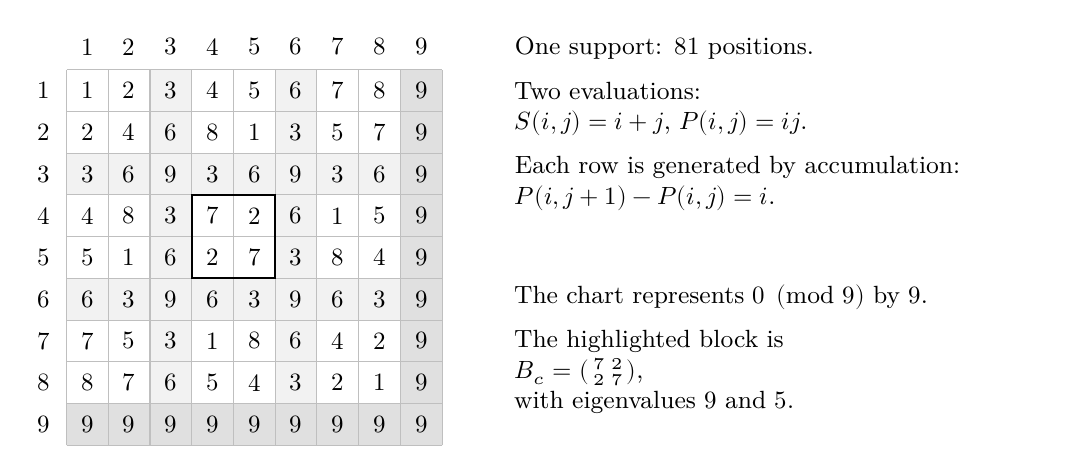
\begin{tikzpicture}[x=.53cm,y=.53cm,font=\small]
\fill[black!5] (1.5,-.5) rectangle (2.5,8.5);
\fill[black!5] (4.5,-.5) rectangle (5.5,8.5);
\fill[black!5] (-.5,2.5) rectangle (8.5,3.5);
\fill[black!5] (-.5,5.5) rectangle (8.5,6.5);
\fill[black!12] (7.5,-.5) rectangle (8.5,8.5);
\fill[black!12] (-.5,-.5) rectangle (8.5,.5);
\foreach \i in {1,...,9}{
 \node at (\i-1,9.05) {\(\i\)};
 \node at (-1.05,9-\i) {\(\i\)};
 \foreach \j in {1,...,9}{
  \pgfmathtruncatemacro{\v}{mod(\i*\j-1,9)+1}
  \node at (\j-1,9-\i) {\(\v\)};
 }
}
\foreach \k in {0,...,9}{
 \draw[black!25] (\k-.5,-.5)--(\k-.5,8.5);
 \draw[black!25] (-.5,\k-.5)--(8.5,\k-.5);
}
\draw[line width=.65pt] (2.5,3.5) rectangle (4.5,5.5);
\node[anchor=west,align=left,text width=6.5cm] at (10,7.2) {One support: \(81\) positions.\\[5pt]Two evaluations:\\ \(S(i,j)=i+j\), \(P(i,j)=ij\).\\[5pt]Each row is generated by accumulation:\\ \(P(i,j+1)-P(i,j)=i\).};
\node[anchor=west,align=left,text width=6.5cm] at (10,1.8) {The chart represents \(0\pmod9\) by \(9\).\\[5pt]The highlighted block is\\ \(B_c=\left(\begin{smallmatrix}7&2\\2&7\end{smallmatrix}\right)\),\\ with eigenvalues \(9\) and \(5\).};
\end{tikzpicture}
\caption{APP multiplication table in positive representatives. Non-unit rows and columns are distinguished by gray shading; the frame identifies the adjacent diagonal block with equal diagonals. The displayed table is an observable of the arithmetic torus; its representation edges do not constitute an intrinsic topological boundary of the torus.}
\label{fig:app}
\end{figure}


\begin{proposition}[Reconstruction of the evaluations]
The two pairs in \eqref{eq:app-levantada} determine \(i+j\) and \(ij\) exactly. The residues alone do not determine these integer evaluations or their quotients.
\end{proposition}
\begin{proof}
The first statement is \eqref{eq:residuo-cociente} applied to each sheet. For the second, \(10=1+9\) and \(19=1+2\cdot9\) have the same residue and different quotients. On the two-dimensional support, positions \((5,5)\) and \((8,2)\) give the same sum and the same product residue, but products \(25=7+18\) and \(16=7+9\). The residue projection identifies data that the lifted evaluation distinguishes.
\end{proof}

\subsubsection{Cayley graph, toroidal topology, and winding number}

The cardinal translations are given, in row and column coordinates, by
\[
 \nu_N=(-1,0),\quad\nu_E=(0,1),\quad
 \nu_S=(1,0),\quad\nu_O=(0,-1),\qquad T_d(x)=x+\nu_d.
\]
The first coordinate increases southwards and the second eastwards. The graph
\[
 \mathscr G_9=\operatorname{Cay}(X_9,\{\nu_N,\nu_E,\nu_S,\nu_O\})
\]
is the two-dimensional cyclic lattice: it has eighty-one vertices and four outgoing oriented edges per vertex. It is a Cayley graph for the \emph{additive} structure of the support. Multiplication of residues has zero divisors and does not turn all APP rows into a multiplicative group.

A cardinal word \(w=d_1\cdots d_r\) and an origin \(x_0\) determine
\[
 x_k=x_0+\sum_{j=1}^k\nu_{d_j}\pmod9.
\]
There are \(81\cdot4^r\) oriented paths of length \(r\), including returns and backtracking. When the path closes, its integer displacement before reduction defines
\begin{equation}
 \operatorname{wind}(w)=\frac19
 \bigl(\#S(w)-\#N(w),\#E(w)-\#O(w)\bigr)\in\ZZ^2.
\end{equation}
Path reversal changes the sign of this vector. Returning to the same residue position therefore does not require the winding to vanish. This is the first example of a distinction that will reappear in phase return: one coordinate may close while another records a nontrivial evolution.

\subsubsection{Transport quotient and cocycle identity}

Let \(s_9:\ZZ/9\ZZ\to D_9\) be the section of positive representatives. The transport quotient associated with additive composition, also called the \emph{carry} in positional arithmetic, is
\[
 c_9(a,b)=\frac{s_9(a)+s_9(b)-s_9(a+b)}9.
\]
The compositional character of this memory is expressed by an exact identity.

\begin{lemma}[Cocycle identity]
For \(a,b,c\in\ZZ/9\ZZ\),
\[
 c_9(a,b)+c_9(a+b,c)=c_9(b,c)+c_9(a,b+c).
\]
\end{lemma}
\begin{proof}
Both sums equal
\[
 \frac{s_9(a)+s_9(b)+s_9(c)-s_9(a+b+c)}9.
\]
Associativity of the sum of lifted representatives requires precisely this additional term when composing in the quotient.
\end{proof}

With positive representatives, this cocycle is not normalized at the identity: \(c_9(0,a)=1\). If \(s_0\) takes representatives in \(\{0,\ldots,8\}\), its normalized carry \(c_0\) satisfies
\[
 c_9(a,b)=c_0(a,b)+\mathbf1_{a=0}+\mathbf1_{b=0}-\mathbf1_{a+b=0}.
\]
The difference is the change of section; it does not alter the cocycle identity. The subsequent decomposition of the calendar into phase and window will use representatives from zero to eight.

The totals of both evaluations distinguish the visible contribution from that retained in the quotient:
\[
 \sum S=810,\quad\sum P=2025,\quad
 \sum\Sigma=405,\quad\sum\Pi=459,
\]
\[
 \sum q^+=45,\qquad\sum q^\times=174.
\]
It follows that
\begin{equation}
 2025-810=(459-405)+9(174-45)=54+9\cdot129.
 \label{eq:defecto-integrado}
\end{equation}
The sum--product difference is not exhausted by the visible defect \(54\). The identity also preserves the quotient defect \(129\). Removing it would change the arithmetic being transported, even if the residue table remained identical.

\subsubsection{Ternary reduction and multiplicative radical}

The ring \(R=\ZZ/9\ZZ\) has unit group \(\{1,2,4,5,7,8\}\) and maximal ideal
\[
 \mathfrak m=(3)=\{0,3,6\},\qquad\mathfrak m^2=0.
\]
Every additive row is a permutation of the nine representatives. A multiplicative row is such a permutation exactly when its index is a unit. Rows three and six contain three repeated values; row nine contains only the representative of the zero class. Thus multiplicative folding already distinguishes the units from the nilpotent sector before any continuous geometry is introduced.

The map \(x\mapsto3x\) has kernel and image both equal to \(\mathfrak m\). It induces an isomorphism of vector spaces over \(\FF_3\),
\[
 R/\mathfrak m\longrightarrow\mathfrak m,\qquad [x]\longmapsto3x,
\]
but not a ring isomorphism. In particular, the visible sequence \(3,6,9\) admits two different readings: its direct reduction modulo three is \(0,0,0\), whereas extracting the factor three and then reducing its internal coordinate gives \(1,2,0\). This second operation preserves a coordinate of the ideal; it is not the same projection as directly reducing the original number.

\subsubsection{Latin realization of the additive evaluation}

The difference between the two evaluations can also be expressed through
operators. Let \((e_r)_{r\in\ZZ/9\ZZ}\) be the orthonormal basis of \(\CC^9\).
The assignment \(v_{ab}=e_{a+b}\) produces an orthonormal basis in every row
and column. The projectors \(P_{ab}=v_{ab}v_{ab}^{*}\) satisfy
\[
 \sum_bP_{ab}=I_9=\sum_aP_{ab},\qquad P_{ab}^2=P_{ab}.
\]
Indeed, each translation \(b\mapsto a+b\) permutes the nine residues.
This yields a realization of a Latin square by rank-one projectors,
in the terminology of quantum Latin squares
\cite{mustovicary,delascuevas2023}. This construction starts from the
additive sheet already defined and makes explicit the map to its operator representation.

The multiplicative evaluation preserves different content: for \(a=3\), the
vectors \(e_{3b}\) repeat the residues \(0,3,6\), and
\[
 \sum_{b\in\ZZ/9\ZZ}|e_{3b}\rangle\langle e_{3b}|
 =3\bigl(|e_0\rangle\langle e_0|+|e_3\rangle\langle e_3|
                    +|e_6\rangle\langle e_6|\bigr).
\]
The multiplicity is recorded in the operator and characterizes the multiplicative
radical. Thus the toroidal support, the Latin property, and the operator
resolution of the identity are properties requiring different definitions.
The quantum magic squares studied by De las Cuevas, Drescher, and Netzer
require positive entries and row and column sums equal to the identity;
their theory also distinguishes dilations with commuting entries\cite{delascuevas2020}.
This reference provides a precise language for comparing realizations of APP.

\subsection{TRIT: orientation and quadratic regimes}

\begin{definition}[Ternary signature and local lift]
The TRIT signature uses the balanced identification
\[
 \FF_3\longrightarrow\TRIT,\qquad 0\mapsto0,\quad1\mapsto+1,\quad2\mapsto-1.
\]
For \(n\in\ZZ\), its lift preserves \(n=r+3c\), where \(r\in\TRIT\) and \(c\in\ZZ\). In a transition of bounded local amplitude, the three states \((0,-1),(0,0),(0,+1)\) may exhibit the same zero residue and different carries.
\end{definition}

The signature does not replace the trajectory. A zero residue does not mean an absence of orientation, phase, or quotient information. Nor does it introduce a physical quantity by itself. Its function is to distinguish algebraically the transport classes that will be realized next.

\subsubsection{Three quadratic regimes and a common exponential}

Once the ternary signature has been obtained, its quadratic realization is defined by
\begin{equation}
 \mathbb A_\tau=\RR[X]/(X^2+\tau),\qquad \tau\in\TRIT.
 \label{eq:algebras-trit}
\end{equation}
If \(J_\tau\) is the class of \(X\), then \(J_\tau^2=-\tau I\). The structure distinguishes the elliptic type \(\tau=+1\), the parabolic type \(\tau=0\), and the hyperbolic type \(\tau=-1\). The real realization does not generate the signature: it expresses the types already produced by oriented reduction.

\begin{proposition}[Exponentiation of the three types]
In each algebra \eqref{eq:algebras-trit},
\begin{equation}
 \exp(tJ_\tau)=C_\tau(t)I+S_\tau(t)J_\tau,
\end{equation}
where
\[
 C_\tau(t)=\sum_{n\ge0}\frac{(-\tau)^nt^{2n}}{(2n)!},\qquad
 S_\tau(t)=\sum_{n\ge0}\frac{(-\tau)^nt^{2n+1}}{(2n+1)!}.
\]
The three realizations are
\[
 \begin{array}{c|c|c}
 \tau&J_\tau^2&\exp(tJ_\tau)\\\hline
 +1&-I&\cos t\,I+\sin t\,J_\tau\\
 0&0&I+tJ_\tau\\
 -1&I&\cosh t\,I+\sinh t\,J_\tau.
 \end{array}
\]
\end{proposition}
\begin{proof}
Separating the even and odd terms of the exponential series and substituting \(J_\tau^{2n}=(-\tau)^nI\) and \(J_\tau^{2n+1}=(-\tau)^nJ_\tau\) gives the formulas. For \(\tau=0\), all terms of degree at least two vanish. In the other two cases, the trigonometric or hyperbolic series are recovered.
\end{proof}

The exponential is common to all three regimes: it is not assigned exclusively to the parabolic branch. The invariants
\[
 C_\tau(t)^2+\tau S_\tau(t)^2=1
\]
follow from \(\exp(tJ_\tau)\exp(-tJ_\tau)=I\). The same algebraic principle preserves unity through realizations that differ in their quadratic type.

In the hyperbolic regime, \(P_\pm=(I\pm J_{-1})/2\) are complementary projectors and
\[
 \exp(tJ_{-1})=e^tP_++e^{-t}P_-.
\]
Growth and contraction appear jointly in two eigendirections. In the elliptic regime, the parameter describes a rotation; in the parabolic regime, a nilpotent translation. The temporal interpretation adopted by HMT associates \(+1\) with return with memory, \(0\) with the threshold, and \(-1\) with bidirectional opening. This interpretation requires an ordering of the parametrization; it does not add a fourth algebraic type.

% Cumulative TRIT extension; inserted before the regime figure.
% It neither replaces nor removes the preceding development.
\subsubsection{Balanced division and composition of lifts}
\label{trit-ampl-div-balanceada}

Ternary reduction expresses an integer evaluation of APP through a visible
coordinate and a prolongation coordinate. Its function is not merely to
abbreviate the notation for an integer: it provides a composition rule
determining how the quotient changes when evaluations are added or multiplied.
The balanced choice also makes the compatibility of this rule with sign
reversal explicit.

\begin{definition}[Balanced ternary coordinates]
\label{trit-ampl-def-coordenadas}
For \(n\in\mathbb Z\), let
\[
 q_3(n)=\left\lfloor\frac{n+1}{3}\right\rfloor,\qquad
 r_3(n)=n-3q_3(n).
\]
The map
\[
 \mathcal B:\mathbb Z\longrightarrow\TRIT\times\mathbb Z,\qquad
 n\longmapsto(r_3(n),q_3(n))
\]
is called the balanced ternary decomposition. Its inverse is
\(\mathcal L(r,c)=r+3c\).
\end{definition}

Indeed, \(r_3(n)\in\{-1,0,+1\}\). If two pairs represent the same integer,
\(r+3c=s+3d\), then \(r-s\) is a multiple of \(3\) and belongs to the interval
\([-2,2]\); necessarily \(r=s\) and \(c=d\). The representation is therefore
unique. Division can be repeated on \(q_3(n)\), so that each level preserves
the data needed to reconstruct the preceding one. The quotient is not a
perturbation of the residue: it is its complementary coordinate.

The signature obtained from an evaluation \(F\), with \(F=S\) or \(F=P\) in APP,
is \(r_3\circ F\). When reduction acts on the phase cursor, the same balanced
section produces the classes \(\{1,4,7\}\), \(\{2,5,8\}\), and
\(\{3,6,9\}\), with values \(+1,-1,0\). The TPK selector defined below
uses these classes to determine the operating mode.
Reading an evaluation and selecting a mode thus share the same ternary
reduction, but have different domains and functions.

\Needspace{16\baselineskip}
\begin{proposition}[Arithmetic of balanced pairs]
\label{trit-ampl-prop-aritmetica}
Let \(n=r+3c\) and \(m=s+3d\), with \(r,s\in\TRIT\). Define
\[
 \chi(r,s)=\frac{r+s-r_3(r+s)}3.
\]
Integer operations are transported to the pairs by
\begin{align}
 (r,c)\boxplus(s,d)
 &=\bigl(r_3(r+s),c+d+\chi(r,s)\bigr),
 \label{trit-ampl-eq-suma}\\
 (r,c)\boxtimes(s,d)
 &=\bigl(rs,rd+sc+3cd\bigr).
 \label{trit-ampl-eq-producto}
\end{align}
The map \(\mathcal L\) preserves both operations.
\end{proposition}
\begin{proof}
The equality \(r+s=r_3(r+s)+3\chi(r,s)\) gives
\[
 n+m=r_3(r+s)+3\bigl(c+d+\chi(r,s)\bigr).
\]
On the other hand,
\[
 nm=rs+3(rd+sc+3cd).
\]
Since the product of two balanced representatives again belongs to
\(\{-1,0,+1\}\), it requires no additional residue reduction. Uniqueness
of the decomposition proves both formulas.
\end{proof}

For example, \(2=(-1)+3\) and \(4=1+3\). Their sum and product are reconstructed
as
\[
 (-1,1)\boxplus(1,1)=(0,2),\qquad
 (-1,1)\boxtimes(1,1)=(-1,3).
\]
The resulting evaluations are \(6\) and \(8\). Adding the quotients suffices
in this additive example; the product involves the cross terms
\(rd\), \(sc\), and \(3cd\). The discrepancy between the two operations
also resides in the prolongation coordinate, not only in the residue.

The term \(\chi\) is a cocycle of the balanced section. If
\(r\oplus s=r_3(r+s)\), it satisfies
\[
 \chi(r,s)+\chi(r\oplus s,t)
 =\chi(s,t)+\chi(r,s\oplus t).
\]
Both sides represent the quotient of the same sum of three integers.
This identity ensures that regrouping the operations does not change the
reconstructed evaluation. At the same time, projection onto the first
component suppresses this accounting: \(1+1=-1+3\), whereas the residue
reading retains only \(-1\). The information removed is determined,
in this case, by \(\chi(1,1)=1\).

The relation with modulus \(9\) preserves a second discrete scale.
The map
\[
 \beta:\TRIT\times\mathbb F_3\longrightarrow\mathbb Z/9\mathbb Z,
 \qquad (r,\bar c)\longmapsto r+3c\pmod9
\]
is well defined and bijective. Changing the representative of \(\bar c\)
adds a multiple of \(9\); conversely, equality of images fixes
\(r\) first, by reduction modulo \(3\), and then \(\bar c\). Addition
transported by this bijection contains the term
\(\chi(r,s)\) from \eqref{trit-ampl-eq-suma}, now reduced modulo \(3\).
Thus the two ternary levels do not compose by independent coordinatewise
addition: normalization of the first level modifies the second.

In particular, the classes \(3\), \(6\), and \(0\) of
\(\mathbb Z/9\mathbb Z\) have first component \(0\), but second components
\(1\), \(2\), and \(0\), respectively. The distinction already observed
between direct reduction and extraction of the ideal coordinate appears
as a property of \(\beta\). Preserving this coordinate prevents the zero
residue sector from being artificially collapsed into a single position.
Modulus \(1000\), used later to organize decimal blocks,
serves a different positional-representation function; its quotient is
preserved through the corresponding division. A change of base preserves
the integer when it retains residue and quotient, whereas coincidence of
residues in different bases does not by itself identify their transport states.

\Needspace{11\baselineskip}
\subsubsection{Inversion, residue class, and non-visible coordinates}
\label{trit-ampl-inversion}

Additive inversion lifts unambiguously:
\[
 \mathcal B(-n)=(-r_3(n),-q_3(n)).
\]
In particular, \(3\), \(0\), and \(-3\) have coordinates
\((0,1)\), \((0,0)\), and \((0,-1)\). They share a zero signature but
represent different evaluations. In a transition restricted to a quotient
of maximum amplitude \(1\), these are the three possibilities of the
visible fiber over zero; in a general integer lift, that fiber contains
all pairs \((0,c)\), with \(c\in\mathbb Z\).

The quotient coordinate recovers the evaluated integer, but does not by
itself recover the trajectory that produced it. Two APP paths may share
evaluation, residue, and quotient while differing in orientation, sequence
of modes, or winding. Thus decomposition \(\mathcal B\) is integrated into
the transport state rather than replacing it. The arithmetic memory of a
division and the memory of a trajectory are related coordinates, not synonyms.

For a signature sequence of length \(n\), oriented reversal is
\[
 C_{\rm rev}(\tau_1,\ldots,\tau_n)
   =(-\tau_n,\ldots,-\tau_1).
\]
Applying it twice restores the sequence. The operation reverses the order
of positions and the sign of each signature; it preserves the length and
the zero positions in reversed order. In the adopted parametrization,
it interchanges return with memory, associated with \(+1\), and bidirectional
opening, associated with \(-1\), while retaining the threshold \(0\).
Transport of the remaining trajectory data is specified by the corresponding
TPK involution.

This signature reversal must be distinguished from conjugation within a
quadratic algebra. The former may change the type \(\tau\); the latter,
constructed below, acts within a type already fixed. This distinction
prevents attributing an algebraic equivalence between different regimes
to a sign reversal.

\subsubsection{Quadratic product, conjugation, and algebraic norm}
\label{trit-ampl-norma}

An element of \(\mathbb A_\tau\) has a unique expression \(aI+bJ_\tau\).
The relation \(J_\tau^2=-\tau I\) determines its product:
\begin{equation}
 (aI+bJ_\tau)(cI+dJ_\tau)
   =(ac-\tau bd)I+(ad+bc)J_\tau.
 \label{trit-ampl-producto-cuadratico}
\end{equation}
This is a real realization of the type already selected. The coordinates
\(a,b\) are not APP residues, and the product
\eqref{trit-ampl-producto-cuadratico} does not replace
\eqref{trit-ampl-eq-producto}; it expresses another operation in the
declared quadratic codomain.

\begin{definition}[Conjugation and algebraic norm]
\label{trit-ampl-def-norma}
Conjugation of type \(\tau\) and its algebraic norm are
\[
 \overline{aI+bJ_\tau}=aI-bJ_\tau,\qquad
 N_\tau(aI+bJ_\tau)=a^2+\tau b^2.
\]
\end{definition}

\begin{proposition}[Multiplicativity and invertibility]
\label{trit-ampl-prop-norma}
For \(z,w\in\mathbb A_\tau\),
\[
 z\bar z=N_\tau(z)I,\qquad
 N_\tau(zw)=N_\tau(z)N_\tau(w).
\]
Moreover, \(z\) is invertible if and only if \(N_\tau(z)\ne0\), in which case
\[
 z^{-1}=\frac{\bar z}{N_\tau(z)}.
\]
\end{proposition}
\begin{proof}
The product of \(aI+bJ_\tau\) and \(aI-bJ_\tau\) is
\((a^2+\tau b^2)I\). Conjugation is multiplicative and the algebra is
commutative, so that
\((zw)\overline{zw}=(z\bar z)(w\bar w)\). If the norm does not vanish,
the stated formula supplies the inverse. Conversely, if \(zw=I\),
multiplicativity implies \(N_\tau(z)N_\tau(w)=1\).
\end{proof}

The quadratic form \(N_\tau\) is positive definite only in the elliptic type.
For \(\tau=0\), it equals \(a^2\), and the element \(J_0\) is nonzero although
its square and norm are zero. For \(\tau=-1\), it equals \(a^2-b^2\);
the nonzero elements \(I+J_{-1}\) and \(I-J_{-1}\) have zero norm and
their product vanishes. Here the algebraic norm is a multiplicative
quadratic form: it does not presuppose a positive vector-space norm.

The three types admit faithful realizations by
\[
 aI+bJ_\tau\longmapsto
 \begin{pmatrix}a&-\tau b\\b&a\end{pmatrix}.
\]
The determinant of this matrix is \(N_\tau(aI+bJ_\tau)\).
The complex structure, the dual-number structure, and the split real
structure are thus represented by a single matrix expression.
Each preserves its own law and zero divisors. The form of signature
\((1,1)\) in the last case admits a Lorentzian interpretation in dimension
\(1+1\); identification of a physical metric additionally requires a
specific space, field, and transport rule.

\subsubsection{Multiplicative conservation and composition of evolutions}
\label{trit-ampl-evoluciones}

The exponential already obtained belongs to the set of norm-one elements:
\[
 N_\tau\bigl(\exp(tJ_\tau)\bigr)=1.
\]
This conservation persists under composition of parameters. Indeed, all
factors are functions of the same generator, and
\[
 \exp(tJ_\tau)\exp(sJ_\tau)=\exp((t+s)J_\tau).
\]
Comparing the two components gives the addition laws
\begin{align}
 C_\tau(t+s)&=C_\tau(t)C_\tau(s)-\tau S_\tau(t)S_\tau(s),\\
 S_\tau(t+s)&=S_\tau(t)C_\tau(s)+C_\tau(t)S_\tau(s).
\end{align}
Conjugation changes \(t\) to \(-t\) and coincides with inversion within
this subgroup. It does not change \(\tau\): it reverses an evolution of
the chosen regime.

In the elliptic type, the preserved form is \(a^2+b^2\), and the exponential
trajectory traverses the unit-norm circle. In the hyperbolic type, the
eigencoordinates are \(u=a+b\), \(v=a-b\), with \(uv=N_{-1}(z)\).
The exponential gives
\[
 (u,v)=(e^t,e^{-t}),\qquad uv=1.
\]
Growth of one coordinate is accompanied by contraction of the other.
Conservation expresses a relation between the two coordinates; it does
not assert that each remains constant.

In the parabolic type,
\[
 (I+tJ_0)(I+sJ_0)=I+(t+s)J_0,\qquad
 (I+tJ_0)^{-1}=I-tJ_0.
\]
The evolution does not stop because \(J_0^2=0\). Nilpotency removes terms
of order at least two, but preserves the linear term that transports
the parameter. The visible symbol \(0\), the zero element of the algebra,
and the nonzero generator \(J_0\) are distinct. This distinction is
necessary to describe the threshold without identifying it with an absence
of state or dynamics.

\begin{proposition}[Composition of affine coordinates]
\label{trit-ampl-prop-pendientes}
In the chart where the scalar component does not vanish, represent a
direction by \(I+uJ_\tau\). If \(1-\tau uv\ne0\), the direction of its
product with \(I+vJ_\tau\) has coordinate
\[
 u\star_\tau v=\frac{u+v}{1-\tau uv}.
\]
\end{proposition}
\begin{proof}
We have
\[
 (I+uJ_\tau)(I+vJ_\tau)
   =(1-\tau uv)I+(u+v)J_\tau.
\]
Dividing by the scalar component gives the stated expression.
\end{proof}

The affine chart preserves the ratio of components, not the scalar factor
divided out. When \(1-\tau uv=0\), the product must be examined before
changing charts: it may have a well-defined direction with zero scalar
component, or be the zero element in the presence of zero divisors.
The composition law still belongs to the full algebra; a coordinate
singularity does not automatically imply a singularity of the object.
This formula will reappear in the elliptic regional reading. Its use
requires retaining the denominator and, where applicable, the normalization factor.

\subsubsection{Transport of type and subsequent realizations}
\label{trit-ampl-puentes}

The algebras \(\mathbb A_{+1}\), \(\mathbb A_0\), and
\(\mathbb A_{-1}\) are not isomorphic as unital real algebras.
The first is a field; the second contains a nonzero nilpotent; the
third has nontrivial idempotents and is isomorphic to
\(\mathbb R\times\mathbb R\). Thus a change of signature organizing a
route cannot be interpreted as an undifferentiated isomorphism between
the three realizations. The TPK preserves the regime index, the domains,
and the effective operator acting at each transition.

In the electron chapter, the pair of projections of the APP sheets
produces a normalized commutator whose square is \(-I\). The same block
contains an involution of square \(I\) and two nilpotent directions.
The joint realization will be proved for that concrete pair of projections;
the preceding classification explains why the three quadratic relations
can appear within one matrix algebra without being identified with one another.

In the exceptional prolongation, the Paley matrix reduced modulo \(3\)
satisfies \(A_W^2=-I_6\). This relation endows the ternary space with
a structure of dimension \(3\) over \(\mathbb F_9\). Its connection to
a real operator root is expressed through the integral presentation
\[
 \mathbb Z[u]/(u^2+1).
\]
Base changes to \(\mathbb F_3\) and \(\mathbb R\) produce representations
of the same relation. Each retains its characteristic, dimension, and
incidence information. Developing the respective operators establishes
the connection, not equality of their cardinalities.

Norm-one conservation consequently describes the quadratic realizations
of evolutions. Conservation of quotients, orientation, and trajectory
belongs to the transported arithmetic state. Both properties participate
in the construction, with different functions: one determines the identities
of the representations; the other makes it possible to compose, reconstruct,
and prolong the operations that give rise to them.


\begin{figure}[htbp]
\centering
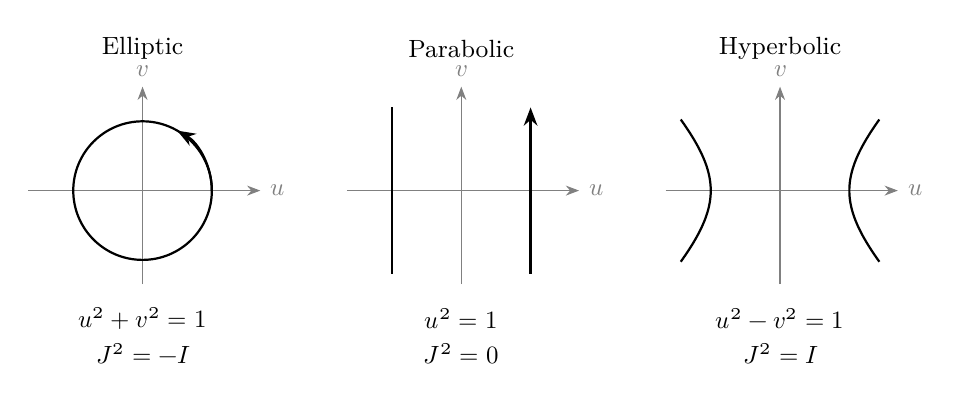
\begin{tikzpicture}[scale=.88,>=Stealth,font=\small]
\foreach \c/\titulo in {0/{Elliptic},4.6/{Parabolic},9.2/{Hyperbolic}}{
\begin{scope}[xshift=\c cm]
\draw[->,gray] (-1.65,0)--(1.7,0) node[right] {\(u\)};
\draw[->,gray] (0,-1.35)--(0,1.5) node[above] {\(v\)};
\node at (0,2.05) {\titulo};
\end{scope}}
\draw[thick] (0,0) circle[radius=1];
\draw[->,thick] (1,0) arc[start angle=0,end angle=60,radius=1];
\node at (0,-1.85) {\(u^2+v^2=1\)};
\node at (0,-2.35) {\(J^2=-I\)};
\draw[thick] (3.6,-1.2)--(3.6,1.2);
\draw[->,thick] (5.6,-1.2)--(5.6,1.2);
\node at (4.6,-1.85) {\(u^2=1\)};
\node at (4.6,-2.35) {\(J^2=0\)};
\draw[thick,domain=-.9:.9,samples=50] plot ({9.2+cosh(\x)},{sinh(\x)});
\draw[thick,domain=-.9:.9,samples=50] plot ({9.2-cosh(\x)},{sinh(\x)});
\node at (9.2,-1.85) {\(u^2-v^2=1\)};
\node at (9.2,-2.35) {\(J^2=I\)};
\end{tikzpicture}
\caption{Quadratic realizations of TRIT. For
\(J_\tau=\left(\begin{smallmatrix}0&-\tau\\1&0\end{smallmatrix}\right)\),
the exponential preserves \(u^2+\tau v^2\). Parabolic degeneration
preserves \(u\) and transports \(v\) linearly. The three diagrams represent
orbits of quadratic forms; their geometric type corresponds to the
algebraic relation of the generator.}
\label{fig:trit-regimenes}
\end{figure}


\newpage
\subsection{TPK: Topological Phase Kernel}

The dynamics uses the phase selector
\[
 M_{\rm ph}(r)=
 \begin{cases}
 +1,&r\in\{1,4,7\},\\
 -1,&r\in\{2,5,8\},\\
 0,&r\in\{3,6,9\}.
 \end{cases}
\]
Its value determines which evaluation operates. Cardinal transport moves the corresponding cursor; the record preserves the previous value, the new quotient, the orientation, and the transition. Selection and transport are therefore different functions: a ternary sign is not a displacement on the torus.

We shall denote by \(\widehat X\) the space of arithmetic states with trajectory memory. An element contains the positions and directions of both cursors, the active mode, the TRIT signature, the phase, the residues and quotients of both evaluations, the carries, the constructed prefix, and the boundary data. When a refinement cylinder is introduced, it forms part of the state. This notation avoids replacing the object by a reduced version that retains only the visible symbol.

\begin{definition}[TPK update]
Let \(\mathsf{Sel}_t\) be mode selection through \(M_{\rm ph}\), \(\mathsf{Tra}_t\) the lifted cardinal transport, and \(\mathsf{Mem}_t\) the record update. The transition is
\begin{equation}
 \mathcal U_t=\mathsf{Mem}_t\circ\mathsf{Tra}_t\circ\mathsf{Sel}_t.
 \label{eq:actualizacion}
\end{equation}
Each application preserves the fields it does not modify and updates the remaining fields by Euclidean division and trajectory concatenation.
\end{definition}

The notation \eqref{eq:actualizacion} expresses the order of composition; it does not replace the effective rules. The following section specifies its finite two-cursor realization completely. Prolongation will then be obtained not by erasing its memory and repeating the first emission, but by transporting the prefixes and their compatible boundaries. Thus APP supplies the evaluations, TRIT distinguishes their regimes, and TPK composes their evolution.

% Expository recovery from the TPK kernel's source owners.
% Provenance and preservation controls are documented in technical/TPK_INTEGRACION.md.
% This file expands the TPK section; it does not replace extension.tex or generacion.tex.

\subsubsection{Dynamic state, observables, and operational dependencies}
\label{tpk-int:estado}

The Topological Phase Kernel organizes the evolution of the two APP sheets
with the orientation determined by TRIT. Its definition comprises the state
on which it acts, the transition rules, and the relations that make
prolongations compatible. Equation \eqref{eq:actualizacion} acquires operational
content when the coordinates received and modified by each factor are specified.
Position belongs to the toroidal support; phase belongs to the calendar;
orientation determines transport; quotients record the arithmetic evaluation
before reduction. These coordinates are related through the transition and
retain different mathematical functions.

The observable projection of a state is
\begin{equation}
 q=(x_+,d_+,x_\times,d_\times,\theta)
 \in\mathcal Q_{\rm obs}
 :=(X_9\times\mathcal D)^2\times\Theta_{108},
 \qquad \mathcal D=\{N,E,S,O\},\quad
 \Theta_{108}=\ZZ/108\ZZ.
 \label{tpk-int:qobs}
\end{equation}
The subscripts distinguish the additive and multiplicative cursors. The
fibers of complete states over \(q\) preserve the ordered trajectory, the
integer evaluations of both sheets, their residues and quotients, and the
orientation and boundary records. A precision prolongation adds the prefix
and the compatible cylinder. Thus two states with the same projection
\(q\) may retain different records.

Operational dependencies have three levels. At the local level, the selector
activates a sheet, transport changes its position, and the update computes
the new arithmetic coordinates. At the trajectory level, these transitions
compose and retain the records of preceding steps. At the refinement level,
extension relations determine which continuation preserves the predecessor's
prefix, signature, and boundary. The finite calendar describes the phase
of these operations; holonomy describes their composition on the history.

\subsubsection{Tritic selection and lifted cardinal transport}
\label{tpk-int:seleccion}

Let \(\bar\theta\in\{0,\ldots,107\}\) be the calendar representative.
The operating phase and the dodecaphase sector are
\begin{equation}
 r(\theta)=1+(\bar\theta\bmod9),\qquad
 \beta(\theta)=\left[\left\lfloor\frac{\bar\theta}{9}\right\rfloor\right]_{12}.
 \label{tpk-int:fase}
\end{equation}
The previously defined selector may be written \(\varepsilon_9=M_{\rm ph}\).
Its value vector in the ordered chart of \(D_9\) is
\[
 m_{\rm ph}=(1,-1,0,1,-1,0,1,-1,0).
\]
The function \(M_{\rm ph}:D_9\to\TRIT\) and this vector are two
presentations of the same selector, with their respective domains.

Define the activation indicators
\[
 a_+(\theta)=\mathbf1_{\{1,4,7\}}(r(\theta)),\qquad
 a_\times(\theta)=\mathbf1_{\{2,5,8\}}(r(\theta)).
\]
Cursor transport is then
\begin{equation}
 x_+'=x_++a_+(\theta)\nu_{d_+},\qquad
 x_\times'=x_\times+a_\times(\theta)\nu_{d_\times}
 \quad\text{in }X_9.
 \label{tpk-int:cursores}
\end{equation}
In phases \(3,6,9\), both positions remain unchanged; the neutral event
forms part of the chronology and its record. Cardinal directions determine
the vectors \(\nu_d\), whereas the phase signature determines which
vector is applied.

The integer lift preserves boundary crossing. If
\(s:X_9\to D_9^2\) chooses positive representatives and
\(x'=x+a\nu_d\), with \(a\in\{0,1\}\), define
\begin{equation}
 b_d(x,a)=\frac{s(x)+a\nu_d-s(x')}{9}\in\ZZ^2.
 \label{tpk-int:borde}
\end{equation}
Divisibility by \(9\) follows from equality in \(X_9\).
If \(z\in\ZZ^2\) records previous crossings, the update is
\(z'=z+b_d(x,a)\). Thus
\[
 s(x')+9z'=s(x)+9z+a\nu_d.
\]
The integer transport data remain reconstructible after the position
has been reduced on the torus.

\begin{proposition}[Conservation of lifted displacement]
\label{tpk-int:prop-desplazamiento}
For a cardinal trajectory of \(n\) steps, with activation indicators
\(a_t\),
\[
 s(x_n)+9z_n=s(x_0)+9z_0+
 \sum_{t=0}^{n-1}a_t\nu_{d_t}.
\]
The same equality is preserved under concatenation of two compatible trajectories.
\end{proposition}
\begin{proof}
The one-step identity is \eqref{tpk-int:borde}. Summing it over the
\(n\) steps cancels the intermediate coordinates. Splitting the summation
interval into two segments produces exactly the concatenation law.
For a closed trajectory, the difference \(z_n-z_0\) is the previously
defined winding number.
\end{proof}

The same principle governs APP evaluations. If a sheet takes the integer
value \(N_t\), its record simultaneously preserves
\(N_t=R_t+9q_t\). The difference between two steps satisfies
\[
 N_{t+1}-N_t=(R_{t+1}-R_t)+9(q_{t+1}-q_t).
\]
Spatial-crossing memory \(z_t\) and arithmetic quotient \(q_t\)
have different definitions; preserving them jointly maintains the
geometric and arithmetic provenance of every transition.

\subsubsection{Two-cursor chronology and composite returns}
\label{tpk-int:cronologia}

The cardinal involution \(\jmath\) interchanges \(N\) with \(S\) and
\(E\) with \(O\). After applying \eqref{tpk-int:cursores}, both
directions are reversed at the end of a block of \(27\) steps.
Writing
\[
 h(\theta)=\mathbf1_{\{0,27,54,81\}}
             ((\bar\theta+1)\bmod108),
\]
the complete rule on the observable projection is
\begin{equation}
 F_{\rm obs}(q)=
 \bigl(x_+',\jmath^{h(\theta)}d_+,
       x_\times',\jmath^{h(\theta)}d_\times,
       \theta+1\bigr).
 \label{tpk-int:fobs}
\end{equation}
The reading that forms the emission uses the positions before transport,
according to the explicit recurrence in Section~\ref{sec:extension}.
The observable update and emission therefore compose in a fixed order.

\begin{proposition}[Reversibility and period of the observable calendar]
\label{tpk-int:periodo}
The map \(F_{\rm obs}\) is a permutation of
\(\mathcal Q_{\rm obs}\) and satisfies \(F_{\rm obs}^{108}=I\).
Within a block of \(54\) steps, positions and directions are restored;
the coordinate in \(\Theta_{108}\) advances by \(54\).
\end{proposition}
\begin{proof}
Given the final state, the preceding phase is first recovered by subtracting
one in \(\Theta_{108}\). That phase determines whether directions were
reversed and which cursor moved. Applying the corresponding involution
and subtracting the cardinal vector uniquely recovers the initial state.

Each interval of \(27\) steps contains nine activations of each cursor.
The following block preserves the activations and reverses the directions,
so the integer displacements cancel over \(54\) steps. The rule has
period \(54\) in its position and orientation increments; the same
cancellation holds for any calendar origin. After \(108\) steps,
\(\theta\) is also restored.
\end{proof}

We reserve
\[
 \mathcal K_{27}=F_{\rm obs}^{27}:
 \mathcal Q_{\rm obs}\longrightarrow\mathcal Q_{\rm obs}
\]
for the iterate of \(27\) transitions. Its fourth iterate is the
identity on the observable state defined in \eqref{tpk-int:qobs}.
Projecting history onto the calendar makes this finite check possible.
The trajectory record, its evaluations, and the new prefixes remain in
the dynamic state on which \(\mathcal U_t\) acts; observable equality
does not reinitialize them.

\subsubsection{Affine memory transport and composition of states}
\label{tpk-int:memoria}

The observable projection admits fibers of arithmetic and geometric data.
Over a configuration \(q\), we write a state in the form
\[
 x=(q,o,h,c,\sigma,C,b,\lambda).
\]
Here \(o\) preserves orientation and sheet; \(h\), residues and
quotients; \(c\), additive transport memory; \(\sigma\), the boundary
signature; \(C\), the precision cylinder; \(b\), its boundary label;
and \(\lambda\), the recorded trajectory. The signature is determined
by a map
\[
 \operatorname{Sig}_q:
 \mathsf H_q\times\mathsf C_q\times\mathsf{Hist}_q
 \longrightarrow\mathsf S_q,
 \qquad \sigma=\operatorname{Sig}_q(h,c,\lambda).
\]
The symbols \(\mathsf H_q,\mathsf C_q,\mathsf{Hist}_q\), and
\(\mathsf S_q\) denote, respectively, the sets of residue--quotient
data, the abelian transport-memory group, the recorded trajectories,
and the boundary signatures. Realizations of this signature are specified
component by component in the regional and terminal constructions.
This dependence prevents treating the signature as a free parameter
once the data producing it are fixed.

The elementary residue--quotient chart is explicit. For
\(n\in\ZZ\), let
\[
 r=1+((n-1)\bmod9),\qquad u=\frac{n-r}{9}.
\]
Then \(n=r+9u\), with \(r\in D_9\) and \(u\in\ZZ\).
Uniqueness follows because two representatives in \(D_9\) congruent
modulo \(9\) are equal. This chart supplies local integer reconstruction.
The precision towers additionally incorporate the truncation maps and
cylinders developed in \ref{sec:extension} and \ref{sec:generacion}.

Let \(\gamma:q\to q'\) be an observable trajectory. Fiber transport
is expressed through maps
\[
 \mathsf H(\gamma):\mathsf H_q\to\mathsf H_{q'},\qquad
 \mathsf C(\gamma):\mathsf C_q\to\mathsf C_{q'},\qquad
 \mathsf{Hist}(\gamma):\mathsf{Hist}_q\to\mathsf{Hist}_{q'}.
\]
The maps respect identities and composition, and
\(\mathsf C(\gamma)\) is an abelian-group homomorphism.
The increment \(k_{\rm tr}(\gamma)\in\mathsf C_{q'}\) satisfies
\begin{equation}
 \begin{split}
 k_{\rm tr}(\operatorname{id}_q)&=0,\\
 k_{\rm tr}(\gamma_2\circ\gamma_1)
 &=k_{\rm tr}(\gamma_2)+
   \mathsf C(\gamma_2)k_{\rm tr}(\gamma_1).
 \end{split}
 \label{tpk-int:cociclo}
\end{equation}
Here \(k_{\rm tr}\) denotes the transport cocycle;
the rational coordinate \(\kappa\) of record \(K\) retains
its notation in the dodecaphase-closure chapter.

Transportable coordinates are updated by
\begin{equation}
 \begin{aligned}
 h'&=\mathsf H(\gamma)h,&
 c'&=\mathsf C(\gamma)c+k_{\rm tr}(\gamma),\\
 \lambda'&=\gamma\circ\lambda,&
 \sigma'&=\operatorname{Sig}_{q'}(h',c',\lambda').
 \end{aligned}
 \label{tpk-int:accion-memoria}
\end{equation}
The second equation is an affine action: the linear term transports
previous memory and the cocycle adds the increment produced by the
trajectory. In the spatial-crossing realization for each cursor separately,
\(\mathsf C(\gamma)=I\) and \(k_{\rm tr}(\gamma)\) is the sum
of the vectors in \eqref{tpk-int:borde}. This concrete instance connects
the abstract law with the cardinal operations already defined.

\begin{proposition}[Compatibility of the update with concatenation]
\label{tpk-int:composicion-memoria}
Updating by \eqref{tpk-int:accion-memoria} along
\(\gamma_1\), followed by updating along \(\gamma_2\),
coincides with updating along \(\gamma_2\circ\gamma_1\).
\end{proposition}
\begin{proof}
For the affine coordinate, two updates give
\[
 c''=\mathsf C(\gamma_2)\mathsf C(\gamma_1)c
       +\mathsf C(\gamma_2)k_{\rm tr}(\gamma_1)
       +k_{\rm tr}(\gamma_2).
\]
Functoriality of \(\mathsf C\) and
\eqref{tpk-int:cociclo} turn this expression into
\(\mathsf C(\gamma_2\circ\gamma_1)c+
k_{\rm tr}(\gamma_2\circ\gamma_1)\).
The statement for \(h\) follows from composition of
\(\mathsf H\), and that for \(\lambda\) from associativity
of trajectories. The final signature agrees because it is evaluated
on the same three reconstructed coordinates.
\end{proof}

The cylinder and its boundary complete this law through the relations
\(\operatorname{Ext}_\gamma\), defined in
\ref{tpk-int:bidireccionalidad}. Their elements determine which of
the preceding updates preserve an admissible prolongation.
States, together with the triples \((\gamma,x,x')\) admitted by
these relations, form a category over observable trajectories:
\[
 (\gamma_2,x',x'')\circ(\gamma_1,x,x')
     =(\gamma_2\circ\gamma_1,x,x'').
\]
The identity of \(x\) is \((\operatorname{id}_q,x,x)\).
Composition preserves arithmetic transport and boundary prolongability
simultaneously. This is the structure in which returns with memory
and successive refinements take place.

\subsubsection{Dodecaphase record, phase, and accumulated memory}
\label{tpk-int:dodecafase}

The \(108\) transitions are distributed over the ordered windows
\[
 E_m=\{9m-8,\ldots,9m\},\qquad 1\leq m\leq12.
\]
The record preserves the phase origin, orientation, and data
produced during each window. Its map is
\[
 \mathcal R_{12}(x)=
 \bigl((E_m,\tau_m,\sigma_m,\kappa_m,\Lambda_m)\bigr)_{m=1}^{12},
\]
where \(\tau_m\) is the window's subroute, \(\sigma_m\) its
orientation, \(\kappa_m\) the integer boundary increment, and
\(\Lambda_m\) the local incidence record. We adopt the chart
developed in \ref{subsec:k-registro-integral}; its window indices
correspond to \(m=\beta+1\).
The domain comprises compatible TPK histories, and the codomain
their oriented temporal records. Composition of segments and their
increments is governed by \eqref{tpk-int:accion-memoria}.
By contrast, the group \(C_{12}\) describes translation of the
window index; \(\Theta_{108}\) preserves the step calendar.
This distinction specifies what is transformed and what is observed
when a cycle is completed.

In coordinates \(\theta=9b+r\), with \(0\leq r<9\), advancing
\(9\) steps preserves \(r\) and increases \(b\) by one.
Addition of phases introduces the quotient
\[
 c_0(r,r')=\left\lfloor\frac{r+r'}9\right\rfloor,
\]
whose cocycle identity ensures associativity of composition.
The finite calendar preserves \([b]_{12}\); a record of turns
preserves \(b\in\ZZ\), or \(b\in\mathbb N_0\) for a
history with fixed origin. Section~\ref{sec:extension} proves
the nonsplit exact sequence \eqref{eq:extension108}. Its function
is to describe the relation between these coordinates before they
are used to construct the signed state.

The signed record receives phase and memory data through the
composition developed in Section~\ref{sec:k-registro}:
\begin{equation}
 R_{\rm sgn}=\Pi_H\circ\mathcal E_{108}^{90,120}
                         \circ\mathcal R_{12}.
 \label{tpk-int:registro-causal}
\end{equation}
Its domain is the terminal state with memory; its output belongs
to \(\ZZ^{12}\). The reversible transformation between this signed
state and \(K\), together with the rational reading of \(K\),
is proved in the corresponding chapter. Record operations precede
these transformations. Reconstructing a record from its cyclic
differences verifies its recoverability; its dynamic provenance
must be preserved through the events that produced it.

For the encoded trace \((d_t)\) retained by the record,
the event reader counts codes \(\{2,4,6,8\}\) in each window
with orientation \((+,+,+,-,-,-,+,+,+,-,-,-)\).
These codes and the cardinal symbols of \(\mathcal D\)
are different record coordinates. Chapter~\ref{sec:k-registro}
develops this reader, the integral decomposition \(1+5+6\),
the congruences characterizing its image, and its exact inverse.
The inversion proof establishes which data this chart preserves;
the definition of \(\mathcal R_{12}\) specifies the oriented
history on which it acts.

\subsubsection{Phase incidence and internal channel construction}
\label{tpk-int:incidencia}

The selector determines three subsets of \(D_9\):
\[
 H_+=\{1,4,7\},\qquad H_-=\{2,5,8\},\qquad H_0=\{3,6,9\}.
\]
Let \(H_{\rm act}=H_+\sqcup H_-\) be the set of active phases
and \(O_{\rm ph}=D_9\setminus\{9\}\) the chart preceding
the marked return. Denote by \(P_2(H_{\rm act})\) the set of
unordered pairs of active phases. Internal incidence is given by
\begin{equation}
 \mathcal F^{\rm ph}_6=H_{\rm act}\times P_2(H_{\rm act}),\qquad
 \mathcal F^{\rm ph}_8=O_{\rm ph}\times P_2(H_{\rm act}),\qquad
 \Theta_{\rm ph}=D_9\times P_2(H_{\rm act}).
 \label{tpk-int:fases90120}
\end{equation}
The indices describe the number of positions in the first component.
The construction uses the phases and calendar origin already fixed;
subsequent exceptional realizations will transport these incidences
to their own domains.

\begin{proposition}[Cardinalities and oriented phase incidence]
\label{tpk-int:cardinales}
The sets in \eqref{tpk-int:fases90120} have cardinalities
\(90,120,135\), respectively. If
\[
 \partial_{\rm ph}=\Theta_{\rm ph}\times\{-1,+1\},\qquad
 E_{\rm ph}=\partial_{\rm ph}\sqcup\{\infty\},\qquad
 L_{\rm ph}=H_0\times P_2(H_{\rm act}),
\]
then
\[
 |\partial_{\rm ph}|=270,\quad |E_{\rm ph}|=271,\quad
 |L_{\rm ph}|=45,\quad
 |\partial_{\rm ph}\sqcup L_{\rm ph}|=315.
\]
Simultaneously translating the phase origin and marked return preserves
all these cardinalities and inclusions.
\end{proposition}
\begin{proof}
There are six active phases, so
\(|P_2(H_{\rm act})|=\binom62=15\). Multiplying by
\(6,8,9\) gives \(90,120,135\). Orientation doubles \(135\);
the return mark adds one element; the three neutral phases give
\(3\cdot15=45\). A calendar translation transports each factor
by a bijection and carries the marked point to its image. Products
and disjoint unions thus preserve the incidence.
\end{proof}

Here the cardinality \(271\) has a phase-incidence realization.
The cubic completion in Section~\ref{sec:extension} has its own
construction of the corona \(1000-729\). The correspondence
between the two realizations must preserve the maps and marks
identifying them, in addition to their cardinality. Likewise,
the selector \(\varepsilon_9\), the incidence \((90,120)\),
and the extractor \(\mathcal E_{108}^{90,120}\) retain the
domains and operations just distinguished.

\subsubsection{Trajectory reversal and conjugate prolongations}
\label{tpk-int:bidireccionalidad}

Bidirectionality begins with an operation on trajectories before scalar
values are assigned to them. For
\(\gamma=(x_0;d_1,\ldots,d_n)\), with endpoint \(x_n\), define
\[
 \operatorname{rev}\gamma
   =(x_n;\jmath d_n,\ldots,\jmath d_1).
\]
The reversed trajectory starts at the endpoint of the original.
Composition satisfies
\[
 \operatorname{rev}^2\gamma=\gamma,\qquad
 \operatorname{rev}(\gamma_2\circ\gamma_1)
   =\operatorname{rev}\gamma_1\circ\operatorname{rev}\gamma_2,
\]
and integer displacement changes sign. These identities follow by
reversing the order of steps and replacing each cardinal vector
with its opposite. For a loop, it follows that
\(\operatorname{wind}(\operatorname{rev}\gamma)
=-\operatorname{wind}(\gamma)\).

On records, reversal also requires transporting the order of components
and the orientation of events. Route reversal and signature conjugation
are distinguishable operations: their composition is specified when
applied to a concrete record. In particular, the regional involution
interchanging closure and propagation components preserves the self-scaling
axis; its formula is given in Section~\ref{mono-ampl:regiones}.
This regional operation acts on a different domain from cardinal
trajectory reversal.

Extensions over a route \(r:q\to q'\) are expressed by
relations between fibers of compatible states. If \(\mathcal F_q\)
denotes the fiber of complete states over \(q\), we require
\[
 \operatorname{Ext}_r\subseteq\mathcal F_q\times\mathcal F_{q'},
 \qquad \Delta_{\mathcal F_q}\subseteq
        \operatorname{Ext}_{\operatorname{id}_q},
\]
\[
 \operatorname{Ext}_{r_2}\circ\operatorname{Ext}_{r_1}
       \subseteq\operatorname{Ext}_{r_2\circ r_1}.
\]
Their composition preserves the evaluations of both sheets, orientation,
quotients, prefix, and boundary. Route reversal does not by itself imply
that every extension relation is a bijection. Conjugate prolongation
is defined on the domain where transport of these data satisfies
the corresponding compatibilities.

\subsubsection{Nonadic holonomy and continuity of refinement}
\label{tpk-int:holonomia}

A phase turn composes transitions on the state with memory:
\begin{equation}
 \Gamma_{9,k}=\mathcal U_{k+8}\circ\cdots\circ\mathcal U_k.
 \label{tpk-int:gamma}
\end{equation}
On an individualized history, this functional composition realizes
the holonomy relation; on the full domain we retain
\(\Gamma_{9,k}\subseteq\widehat X_k\times\widehat X_{k+9}\),
with the admissible prolongations developed later.
The cyclic base has nine phases, while the fiber preserves trajectory,
quotients, and boundary. Monodromy is the action of one turn of this
base on the fibers; holonomy \(\Gamma_{9,k}\) expresses its
realization through the effective TPK transitions.

If \(g\) observes phase and \(M\) the number of retained turns,
\[
 g(\Gamma_{9,k}x)=g(x),\qquad M(\Gamma_{9,k}x)=M(x)+1.
\]
The first identity expresses phase closure and the second identifies
the new temporal depth. Coinductive prolongation also preserves its
cylinders and prefixes. Restrictions between depths compose an inverse
system; a compatible section gathers its antecedents without replacing
them by the latest observation. This arithmetic of histories and its
unity are developed in \ref{hist:seccion}--\ref{hist:doble-varianza};
the regions and their readers are constructed in Section~\ref{sec:generacion}.

Phase transfer on emissions already constructed has a different domain.
Let \(\mathcal A_+\) and \(\mathcal A_\times\) be the
additive and multiplicative signature alphabets, with cardinalities
\(18\) and \(26\). Their product identifies the catalog \(\mathcal U_6\).
For \(f:\mathcal A_+\times\mathcal A_\times\to\RR\),
the sheet averages are
\[
 (E_+f)(s,e)=\frac1{18}\sum_{s'\in\mathcal A_+}f(s',e),\qquad
 (E_\times f)(s,e)=\frac1{26}\sum_{e'\in\mathcal A_\times}f(s,e').
\]
These emissions and their cardinalities are constructed through the
recurrence in Section~\ref{sec:extension}. Once they have been obtained,
the transfer operator is defined on
\(\mathcal U_6\times C_9\) by
\[
 P_+=E_+,\quad P_-=E_\times,\quad P_0=I,\qquad
 \mathcal K_{\rm ph}((u,r),(v,r+1))=P_{M_{\rm ph}(r)}(u,v),
\]
with zero weight for all other phase transitions. The index
\(r\) uses the positive representative of the cyclic class.
The phase order \((+1,-1,0)^3\) then produces the renewal
\[
 \mathcal K_{\rm ph}^{9}\big|_r=E_+E_\times.
\]
Indeed, both averages are idempotent, commute, and average different
factors; their composition assigns weight \(1/(18\cdot26)=1/468\)
to each emission. This equality characterizes a subsequent transfer
observable. History transport remains given by \eqref{tpk-int:gamma},
with its memory and boundary.

The resulting hierarchy establishes the function of the following chapters.
Finite emission constructs the domain and regions; extension relations
preserve their prefixes; the nonadic connection prolongs them; the
dodecaphase record determines the data entering \(K\) and the
closure of \(\alpha\). Numerical and incidence realizations receive
this preceding structure. This order allows every consequence to be
presented in its own chapter while preserving, from the formal kernel
onwards, the objects that make it possible.


\subsection{Accumulated memory and transport resolvents}
\label{subsec:memoria-resolvente}

Calendar return does not remove increments produced during the journey.
To express this distinction in operator form, an accumulated trajectory-event
record is constructed first, followed by its generating series. Reduction
of memory variables will be performed on this transport, also preserving
the source and output reader.

\subsubsection{Oriented events and record update}

Let \((d_t)\) be the sequence of integer direction codes retained by
a TPK trajectory. The code \(d_t\) and the cursor's cardinal direction
are different coordinates; no identification of their alphabets is assumed.
We number the windows starting from zero:
\[
 I_m=\{9m+1,\ldots,9m+9\},\qquad m\geq0.
\]
In the first cycle, \(I_m\) is window \(E_{m+1}\) of the
dodecaphase record. Its orientation is
\[
\sigma=(1,1,1,-1,-1,-1,1,1,1,-1,-1,-1).
\]
For a prolonged history, \(\sigma_m\in\{-1,1\}\) is the sign
retained in the corresponding window. The signed event is
\begin{equation}
 a_m=\sigma_m\sum_{t\in I_m}
       \mathbf1_{\{2,4,6,8\}}(d_t),\qquad |a_m|\leq9.
 \label{mem:evento}
\end{equation}
Each summand is incorporated when its transition occurs. This definition
counts trace events; it does not select directions through a value
that is to be obtained later.

Let \(\mathbf e_0,\ldots,\mathbf e_{11}\) be the basis of \(\ZZ^{12}\)
and \(S\mathbf e_j=\mathbf e_{j+1\bmod12}\). Write
\(R=S^{-1}\). The accumulated record in fixed coordinates satisfies
\[
z_{m+1}=z_m+a_m\mathbf e_{m\bmod12}.
\]
A prefix with no accumulated history starts at \(z_0=0\); at a different
origin, \(z_0\) retains the preceding record.
The frame accompanying the calendar is \(y_m=S^{-m}z_m\).

\begin{proposition}[Update and return with memory]
\label{mem:prop-actualizacion}
The record in the moving frame satisfies
\begin{equation}
 y_{m+1}=Ry_m+\eta_m,\qquad
 \eta_m=a_mR\mathbf e_0.
 \label{mem:actualizacion}
\end{equation}
For every \(n\geq1\),
\begin{equation}
 y_n=R^ny_0+\sum_{j=0}^{n-1}R^{n-1-j}\eta_j.
 \label{mem:iteracion}
\end{equation}
In particular,
\begin{equation}
 y_{12}=y_0+\sum_{j=0}^{11}a_j\mathbf e_j.
 \label{mem:retorno12}
\end{equation}
\end{proposition}
\begin{proof}
Multiplying the update of \(z_m\) by \(S^{-(m+1)}\) gives
\(y_{m+1}=S^{-1}y_m+a_mS^{-1}\mathbf e_0\), since
\(S^{-m}\mathbf e_{m\bmod12}=\mathbf e_0\).
Formula \eqref{mem:iteracion} follows by induction.
For \(n=12\), \(R^{12}=I\) and
\(R^{11-j}\eta_j=a_jR^{12-j}\mathbf e_0=a_j\mathbf e_j\),
which proves \eqref{mem:retorno12}.
\end{proof}

Thus twelve windows restore the frame and preserve the event vector.
The count alone does not recover the order of all steps within each
window; that order remains in the recorded trajectory.

To specify the balance, define
\[
 D_3=I-S^3,\quad D_4=I-S^4,\quad
 B=D_3^{\mathsf T}D_3+D_4^{\mathsf T}D_4,
\]
\[
 \mathcal M(y)=\tfrac12y^{\mathsf T}By,
 \qquad q(y)=\sum_{j=0}^{11}y_j.
\]
The first is a quadratic form of the record; the second records the sum
of its coordinates. They are not identified here with physical energy or charge.

\begin{proposition}[Event-induced balance]
\label{mem:prop-balance}
Update \eqref{mem:actualizacion} satisfies
\begin{equation}
 \begin{aligned}
 \mathcal M(y_{m+1})-\mathcal M(y_m)
   &=a_m(By_m)_0+2a_m^2,\\
 q(y_{m+1})-q(y_m)&=a_m.
 \end{aligned}
 \label{mem:balance}
\end{equation}
\end{proposition}
\begin{proof}
Expanding the products gives
\(B=4I-S^3-S^{-3}-S^4-S^{-4}\); hence
\(R^{\mathsf T}BR=B\) and \(B_{00}=4\).
Since \(y_{m+1}=R(y_m+a_m\mathbf e_0)\), the quadratic difference
is \(a_m\mathbf e_0^{\mathsf T}By_m+\tfrac12a_m^2B_{00}\).
The coordinate sum is invariant under permutation \(R\),
giving the second equality.
\end{proof}

\Needspace{20\baselineskip}
\subsubsection{Generating series and uniform memory control}

The series preserves all increments, not only their sum at the end of
a cycle. With a formal variable \(u\), let
\[
 Y(u)=\sum_{m\geq0}y_mu^m,\qquad
 H_\eta(u)=\sum_{m\geq0}\eta_mu^m.
\]

\begin{proposition}[Resolvent and tail bound]
\label{mem:prop-serie}
The formal identity
\begin{equation}
 Y(u)=(I-uR)^{-1}\bigl(y_0+uH_\eta(u)\bigr)
 \label{mem:serie}
\end{equation}
holds. Both series converge for \(|u|<1\). If \(\ell:\RR^{12}\to\RR\)
is linear, \(L=\|\ell\|_{1\to\RR}\), \(M_0=\|y_0\|_1\), and
\(0<r<1\), then, for every integer \(N\geq0\) and \(|u|\leq r\),
\begin{equation}
 \left|\sum_{m>N}\ell(y_m)u^m\right|
 \leq Lr^{N+1}\left(
 \frac{M_0+9(N+1)}{1-r}+\frac{9r}{(1-r)^2}\right).
 \label{mem:cota}
\end{equation}
The derivative series converges uniformly on every disk
\(|u|\leq r<1\).
\end{proposition}
\begin{proof}
Multiplying \eqref{mem:actualizacion} by \(u^{m+1}\) and summing gives
\(Y-y_0=uRY+uH_\eta\). The constant term of \(I-uR\) is
invertible, so its formal inverse is \(\sum_{k\geq0}u^kR^k\).
Moreover, \(R\) preserves the \(\ell^1\) norm and
\(\|\eta_m\|_1\leq9\), whence
\(\|y_m\|_1\leq M_0+9m\).
For the tail, sum the majorants
\(L(M_0+9m)r^m\), using
\[
 \sum_{m>N}r^m=\frac{r^{N+1}}{1-r},\qquad
 \sum_{m>N}mr^m=r^{N+1}
 \left(\frac{N+1}{1-r}+\frac r{(1-r)^2}\right).
\]
Finally, \(\sum_{m\geq1}Lm(M_0+9m)r^{m-1}<\infty\)
majorizes the derivative series and proves its uniform convergence.
\end{proof}

The variable \(u\) counts windows of nine transitions. Identifying it
with another reader's variable requires preserving that clock and the
map relating the two readings.

\subsubsection{Memory elimination: operator, source, and reader}

On a domain where the update is fixed as \(U:X\to X\),
the free vector space \(V=\QQ^{(X)}\) on the states admits the operator
\(T\delta_x=\delta_{U(x)}\). The clock is included in \(x\) if
the transition depends on it. This linear extension preserves distinct
states even when they share an observable phase.

Consider a decomposition \(V=V_0\oplus V_1\), where \(V_1\)
is the auxiliary sector to be eliminated, and write
\[
 T=\begin{pmatrix}A&B_1\\C&D\end{pmatrix},\qquad
 v=\binom{v_0}{v_1},\qquad \ell=(\ell_0,\ell_1).
\]
Here \(A:V_0\to V_0\), \(B_1:V_1\to V_0\),
\(C:V_0\to V_1\), and \(D:V_1\to V_1\).
The following identities are formal; they also hold wherever the
resolvents converge.

\begin{proposition}[Schur reduction with source and reader]
\label{mem:prop-schur}
Let
\[
 D_u=(I-uD)^{-1},\qquad
 \mathscr F(u)=I-uA-u^2B_1D_uC.
\]
The retained component of \((I-uT)^{-1}v\) is
\begin{equation}
 w_0=\mathscr F(u)^{-1}\bigl(v_0+uB_1D_uv_1\bigr),
 \qquad w_1=D_u(v_1+uCw_0).
 \label{mem:schur-fuente}
\end{equation}
Its complete reading satisfies
\begin{equation}
 \begin{split}
 \ell(I-uT)^{-1}v
 ={}&(\ell_0+u\ell_1D_uC)
       \mathscr F(u)^{-1}(v_0+uB_1D_uv_1)\\
    &+\ell_1D_uv_1.
 \end{split}
 \label{mem:schur-lector}
\end{equation}
\end{proposition}
\begin{proof}
The two equations of \((I-uT)w=v\) are
\(w_0=v_0+uAw_0+uB_1w_1\) and
\(w_1=v_1+uCw_0+uDw_1\).
Solving the second and substituting it into the first gives
\eqref{mem:schur-fuente}; applying \(\ell_0\) and \(\ell_1\)
to the two components gives \eqref{mem:schur-lector}.
All formal inverses exist because their constant terms are identities.
\end{proof}

The term \(u^2B_1D_uC=\sum_{k\geq0}u^{k+2}B_1D^kC\)
describes departure into memory, \(k\) steps within it, and a return.
By contrast, \(u\ell_1D_uC\) reads memory before that return.
Thus reducing only the operator does not necessarily preserve the
observation: the source and reader must also be transformed.

The distinction is visible in the cycle already constructed. If \(P\)
retains \(\mathbf e_0\), then \(PRP=0\), but
\begin{equation}
 \left\langle\mathbf e_0,(I-uR)^{-1}\mathbf e_0\right\rangle
 =\frac1{1-u^{12}},\qquad
 \left\langle\mathbf e_{11},(I-uR)^{-1}\mathbf e_0\right\rangle
 =\frac u{1-u^{12}}.
 \label{mem:ejemplo-ciclo}
\end{equation}
Indeed, \(R^n\mathbf e_0=\mathbf e_{-n\bmod12}\): the two
series collect, respectively, \(n\equiv0\) and
\(n\equiv1\pmod{12}\). The resolvent of the compression is \(I\),
whereas compression of the resolvent preserves the omitted returns.
This example concerns the twelve-window record, not the entire TPK state.

\subsubsection{Segment composition and coherence of reduction}

Let three composable affine transports be
\(F_i(y)=R_i y+b_i\), with compatible domains and codomains.
The memory produced by the complete journey is
\begin{equation}
 F_3F_2F_1(y)
 =R_3R_2R_1y+b_3+R_3b_2+R_3R_2b_1.
 \label{mem:cociclo-tres}
\end{equation}
The proof is successive substitution of the three affine formulas.
Grouping the first two segments first, or the last two, produces the
same expression; the factors transport each increment from its point
of origin. In \eqref{mem:actualizacion},
\(R_i=R\) and \(b_i\) is the event of its window.

Eliminating several layers preserves a similar coherence.
To make it explicit, now decompose
\(V=V_0\oplus V_1\oplus V_2\) and write
\[
 T=\begin{pmatrix}
 A&B_1&B_2\\C_1&D_{11}&D_{12}\\C_2&D_{21}&D_{22}
 \end{pmatrix},\qquad Q_2=(I-uD_{22})^{-1}.
\]
Eliminating the third component leaves the four blocks
\begin{equation}
 \begin{aligned}
 A'&=A+uB_2Q_2C_2,&
 B_1'&=B_1+uB_2Q_2D_{21},\\
 C_1'&=C_1+uD_{12}Q_2C_2,&
 D_{11}'&=D_{11}+uD_{12}Q_2D_{21}.
 \end{aligned}
 \label{mem:schur-intermedio}
\end{equation}

\begin{proposition}[Transitivity of elimination]
If \(D_*=(D_{ij})_{i,j=1}^2\), the complement obtained in two stages
coincides with that obtained by eliminating both memories together:
\begin{equation}
 \begin{split}
 I-uA'-u^2B_1'(I-uD_{11}')^{-1}C_1'
 ={}&I-uA\\
 &-u^2(B_1\ B_2)(I-uD_*)^{-1}\binom{C_1}{C_2}.
 \end{split}
 \label{mem:schur-transitivo}
\end{equation}
\end{proposition}
\begin{proof}
Solving the third equation of \((I-uT)w=v\) and substituting it into
the first two produces \eqref{mem:schur-intermedio}. Eliminating the
second component then gives the left-hand side of
\eqref{mem:schur-transitivo}. Solving the two memory equations
together gives the right-hand side, by Proposition~\ref{mem:prop-schur}.
The formal solution is unique because \(I-uT\) has constant term
\(I\). Both procedures also transform the source and reader according
to \eqref{mem:schur-fuente}--\eqref{mem:schur-lector}.
\end{proof}

Balance \eqref{mem:balance} describes record increments.
The preceding identities allow them to be transported when memory is
reused in dodecaphase closure; they do not by themselves determine
additional analytic coefficients.


% Verbatim recovery from nucleo.tex REV08, lines 10--32.
% Extension specific to II, placed after the unchanged common kernel.
\subsection{Correspondence between positional support and the oriented calendar}
\label{ii:ampliacion-posicional-calendario}

The calendar representation distinguishes the positions of APP from the
oriented transitions of its evolution. We revisit this correspondence to
make explicit the reading of the segment containing the junction between turns.

Consider the alphabet of nine indices
\[
 D_9=\{1,2,3,4,5,6,7,8,9\}.
\]
Its horizontal and vertical arrangement produces the eighty-one positions
of \(D_9^2\). The oriented cycle \(C_9\) is also used to describe
motion. Its nine edges are assigned, in order, the indices of
\(D_9\). The index of an edge specifies a transition between states,
whereas a vertex specifies its boundary. The map assigning
each edge its index allows the same alphabet to be used in the positional
support and in the calendar; it preserves the distinction between position,
oriented interval, and transported state.

In the integer lift of the calendar, the first turn comprises
the nine consecutive intervals \([0,1],\ldots,[8,9]\). The continuation
\([9,10]\) starts the next turn with index one and updated
memory. The segment drawn up to ten shows both turns at their
junction. This representation specifies the nine transitions of
one turn and the following transition; the holonomy of the state is constructed
subsequently through the effective composition of the TPK.

\begin{figure}[htbp]
\centering
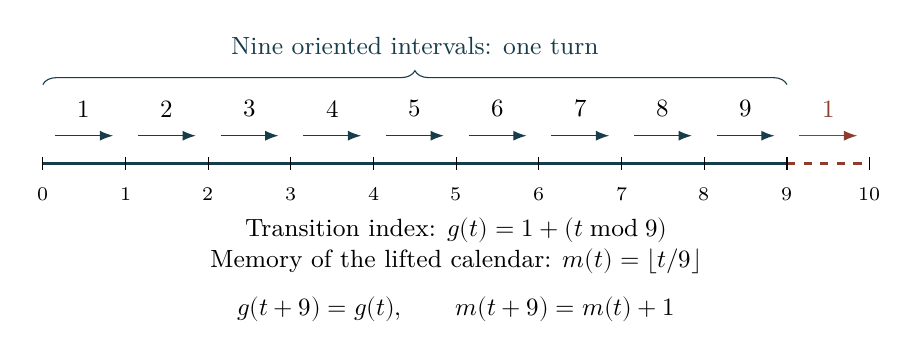
\begin{tikzpicture}[x=1.05cm,y=1cm,>=Latex,font=\small]
 \draw[very thick,ink] (0,0)--(9,0);
 \draw[very thick,dashed,accent] (9,0)--(10,0);
 \foreach \x in {0,...,10}{
   \draw (\x,-.08)--(\x,.08);
   \node[below=5pt,font=\scriptsize] at (\x,0) {$\x$};
 }
 \foreach \x in {1,...,9}{
  \draw[->,ink] (\x-.85,.35)--(\x-.15,.35);
  \node[above=3pt] at (\x-.5,.35) {$\x$};
 }
 \draw[->,accent] (9.15,.35)--(9.85,.35);
 \node[above=3pt,text=accent] at (9.5,.35) {$1$};
 \draw[decorate,decoration={brace,amplitude=5pt},ink] (0,1)--(9,1)
  node[midway,above=7pt] {Nine oriented intervals: one turn};
 \node[align=center] at (5,-1.05)
  {Transition index: $g(t)=1+(t\bmod9)$\\
   Memory of the lifted calendar: $m(t)=\lfloor t/9\rfloor$};
 \node[align=center] at (5,-1.85)
  {$g(t+9)=g(t),\qquad m(t+9)=m(t)+1$};
\end{tikzpicture}
\caption{Lift of the cycle of nine transitions. The upper numbers
label oriented intervals; the lower numbers locate their boundaries.
The dashed interval shows the first transition of the next turn.
The phase index returns and the calendar quotient increases. This diagram
represents the calendar; the action on residues, quotients, orientation,
boundary, and memory is defined through the operations of the TPK.}
\label{fig:ii-segmento-generador}
\end{figure}


% Cumulative fragment to insert after the presentation of the
% TPK update in nucleo.tex. Does not replace nucleo, extension,
% generacion, or registro_k. Detailed provenance in the companion MD.
\subsection{Operator architecture of transport, memory, and prolongation}
\label{ii:tpk-arquitectura}

The topological phase kernel organizes the evolution of the two APP
evaluations on oriented histories. Its structure brings together a path support,
local update rules, prolongation relations, temporal
records, and reading maps. Each component has its own
domain. This hierarchy allows the observable position, the transport
quotient, and the memory of the crossed boundaries to be preserved within
a single construction. The composition in equation~\eqref{eq:actualizacion}
thus acquires a precise realization at each of these levels.

\subsubsection{Bivariate paths and lifted transport}

Let \(\mathsf P_{\rm APP}\) be the free category of the cardinal graph on
\(X_9=(\mathbb Z/9\mathbb Z)^2\). Its objects are the APP positions;
its morphisms are cardinal words, with composition by
concatenation. The category
\[
 \mathsf P_{\rm APP}^{(2)}
 =\mathsf P_{\rm APP}\times\mathsf P_{\rm APP}
\]
preserves, in order, the path of the additive sheet and that of the
multiplicative sheet. Both paths traverse the same arithmetic support and
keep their evaluations distinct.

In the chart \(I_9=\{0,\ldots,8\}\), the generators are
\[
 \nu_N=(-1,0),\quad\nu_E=(0,1),\quad
 \nu_S=(1,0),\quad\nu_O=(0,-1),
 \qquad T_d(x)=[x+\nu_d]_9.
\]
For \(w=d_1\cdots d_r\), the lift to the integer covering space preserves
\[
 \widetilde x_k=\widetilde x_0+\sum_{j=1}^{k}\nu_{d_j},
 \qquad x_k=[\widetilde x_k]_9.
\]
When \(x_r=x_0\), the winding class is
\begin{equation}
 \operatorname{wind}(w)
 =\frac{1}{9}(\#S-\#N,\#E-\#O)\in\mathbb Z^2.
 \label{ii:tpk-enrollamiento}
\end{equation}
The final position and winding are two different readings of the
same route. The second records the displacement of the lift even
when the first has returned.

Path reversal has a determined domain and codomain:
\[
 \operatorname{rev}:\operatorname{Hom}(x,y)
 \longrightarrow\operatorname{Hom}(y,x),\qquad
 d_1\cdots d_r\longmapsto\overline d_r\cdots\overline d_1,
\]
where \(\overline N=S\), \(\overline E=O\). It satisfies
\(\operatorname{rev}^2=I\), reverses the order of composition, and changes the
sign of~\eqref{ii:tpk-enrollamiento}. This is the precise operation that
must be transported when comparing conjugate orientations of a route.

\subsubsection{Full state and preservation through updates}

The description of \(\widehat X\) is organized over the positions and
directions of the two cursors. Over each observable configuration
\(q\), the arithmetic fiber is written
\begin{equation}
 \mathcal F_q=
 \mathsf O_q\times\mathsf H_q\times\mathsf C_q\times
 \mathsf S_q\times\mathsf B_q\times\symup{\Lambda}_q.
 \label{ii:tpk-fibra}
\end{equation}
The coordinates \(\mathsf O_q\) preserve orientation and sheet;
\(\mathsf H_q\), the remainders and quotients of the evaluations;
\(\mathsf C_q\), compatible carries;
\(\mathsf S_q\), the boundary signature;
\(\mathsf B_q\), the prefix and its cylinders; and
\(\symup{\Lambda}_q\), the ordered transport record. The fiber is
restricted by the corresponding arithmetic, incidence, and
truncation identities. The full state also preserves the route
that produced it and the origin from which its phases are read.

Mode selection has type
\[
 M_{\rm ph}:D_9\longrightarrow\{-1,0,+1\},\qquad
 \mathsf{Sel}_t:\widehat X\longrightarrow\widehat X^{\rm sel}_t.
\]
The second map incorporates the value of the first into the state and
activates the corresponding sheet. Lifted transport
\[
 \mathsf{Tra}_t:\widehat X^{\rm sel}_t
 \longrightarrow\widehat X^{\rm tra}_t
\]
applies \(T_d\) to the active cursor, concatenates its route letter, and preserves the
selected sheet. Finally,
\[
 \mathsf{Upd}_t:\widehat X^{\rm tra}_t\longrightarrow\widehat X
\]
updates the evaluations and records. In this notation,
\(\mathsf{Upd}_t\) is the update \(\mathsf{Mem}_t\) of
\eqref{eq:actualizacion}, made explicit in its components.

Each integer evaluation \(a\) is preserved through
\(a=\rho_9(a)+9q_9(a)\); each ternary evaluation, through its oriented
remainder and carry. For a concatenation \(r_2r_1\), carry
transport satisfies the cocycle law
\begin{equation}
 k_{\rm tr}(r_2r_1)
 =k_{\rm tr}(r_2)+\mathsf C(r_2)k_{\rm tr}(r_1),
 \label{ii:tpk-cociclo-transporte}
\end{equation}
where \(\mathsf C(r_2)\) is the transport action of the second route
on the carry coordinate of the first. In the ordered record,
updating is performed by adjoining the event produced:
\[
 \Lambda_{t+1}=\Lambda_t\Vert
 (\text{sheet},d_t,\text{remainder},\text{quotient},
   \text{carry},\text{orientation},\text{boundary})_t.
\]
Preservation has a dynamic meaning here: earlier contributions
remain recoverable within the record being prolonged.
Their coordinates may change when the state is transported.

\subsubsection{Affine action on transport memory}

For a trajectory \(r:q\to q'\), the maps
\[
 \mathsf H(r):\mathsf H_q\to\mathsf H_{q'},\qquad
 \mathsf C(r):\mathsf C_q\to\mathsf C_{q'}
\]
respect identity and concatenation; \(\mathsf C_q\) is the abelian
group of transport memory, and \(\mathsf C(r)\) its homomorphism.
The increment \(k_{\rm tr}(r)\in\mathsf C_{q'}\), with
\(k_{\rm tr}(\operatorname{id}_q)=0\), is the cocycle of
\eqref{ii:tpk-cociclo-transporte}. This symbol distinguishes the transport
increment from the rational coordinates of the dodecaphasic record.

In a chart with data \((h,c,\lambda)\), the update has the
explicit form
\begin{equation}
 h'=\mathsf H(r)h,\qquad
 c'=\mathsf C(r)c+k_{\rm tr}(r),\qquad
 \lambda'=r\circ\lambda.
 \label{ii:tpk-accion-afin}
\end{equation}
The signature is evaluated through
\(\operatorname{Sig}_{q'}(h',c',\lambda')\). Its residence in the
fiber \(\mathsf S_{q'}\) preserves its dependence on those data.

\begin{proposition}[Composition of affine memory]
\label{ii:tpk-composicion-afin}
Updating by \(r_1\), followed by updating by
\(r_2\), agrees with updating by \(r_2r_1\).
\end{proposition}
\begin{proof}
Two memory updates give
\[
 c''=\mathsf C(r_2)\mathsf C(r_1)c
       +\mathsf C(r_2)k_{\rm tr}(r_1)+k_{\rm tr}(r_2).
\]
Compatibility of \(\mathsf C\) with concatenation and
identity~\eqref{ii:tpk-cociclo-transporte} turn this expression
into \(\mathsf C(r_2r_1)c+k_{\rm tr}(r_2r_1)\).
The coordinate \(h\) satisfies the same compatibility by
functoriality of \(\mathsf H\); the trajectory does so by
associativity. The signature agrees because it is evaluated on the same data.
\end{proof}

The spatial chart of each cursor provides an elementary realization
of this law. For \(x\in I_9^2\) and a cardinal direction \(d\),
\[
 a_d(x)=\frac{x+\nu_d-T_d(x)}9\in\mathbb Z^2,
 \qquad x'=T_d(x),\qquad c'=c+a_d(x).
\]
Here \(\mathsf C(r)=I\), and \(k_{\rm tr}(r)\) sums the
integer boundary crossings. For a route of length \(n\),
the telescoping sum gives
\[
 x_n=x_0+\sum_{j=1}^n\nu_{d_j}
             -9\sum_{j=1}^n a_{d_j}(x_{j-1}).
\]
On a loop, the last sum equals
\(\operatorname{wind}(r)\). The residual position returns while
the lift preserves the number and orientation of its crossings.
The remaining memory components retain their own transport
maps and prolongation relations.

\subsubsection{Chronology of the two cursors and observable return}

The finite calendar lives in \(\Theta_{108}=\mathbb Z/108\mathbb Z\).
For \(0\leq\widetilde\theta<108\), set
\[
 r(\theta)=1+(\widetilde\theta\bmod9),\qquad
 \beta(\theta)=\left[\left\lfloor\frac{\widetilde\theta}{9}
 \right\rfloor\right]_{12},\qquad
 \varepsilon_9(r)=M_{\rm ph}(r).
\]
Presentation~\eqref{tpk-int:qobs} groups position and direction by
cursor. This extension groups the two positions first and
then the two directions. The two charts are identified through the
factor permutation
\begin{equation}
 \begin{aligned}
 \mathfrak p_{\rm obs}:\ (X_9\times\mathcal D)^2\times\Theta_{108}
 &\longrightarrow X_9^2\times\mathcal D^2\times\Theta_{108},\\
 (x_+,d_+,x_\times,d_\times,\theta)
 &\longmapsto(x_+,x_\times,d_+,d_\times,\theta),
 \end{aligned}
 \label{ii:permutacion-coordenadas-observables}
\end{equation}
with \(\mathcal D=\{N,E,S,O\}\). The inverse restores each direction alongside
its cursor. If superscripts \({\rm agr}\) and \({\rm sep}\) distinguish
these two expressions of the observable successor, then
\[
 \mathfrak p_{\rm obs}F_{\rm obs}^{\rm agr}
 =F_{\rm obs}^{\rm sep}\mathfrak p_{\rm obs}.
\]
Indeed, the selector depends on the same phase, the cardinal vector is
applied to the same cursor, and direction reversal occurs at the same
instant; only the coordinate order changes. We retain
\(\mathcal Q_{\rm obs}\) and \(F_{\rm obs}\) for the space and
map so identified. This presentation permutation leaves
the events and memory coordinates of the history unchanged.

The observable space is
\[
 \mathcal Q_{\rm obs}
 =X_9^2\times\{N,E,S,O\}^2\times\Theta_{108}.
\]
Write a state as
\(q=(x_+,x_\times,d_+,d_\times,\theta)\). The active sheet is first evaluated
at the current position. The positions are then updated by
\begin{equation}
 (x_+',x_\times')=
 \begin{cases}
 (T_{d_+}x_+,x_\times),&\varepsilon_9(r)=+1,\\
 (x_+,T_{d_\times}x_\times),&\varepsilon_9(r)=-1,\\
 (x_+,x_\times),&\varepsilon_9(r)=0.
 \end{cases}
 \label{ii:tpk-fobs-posiciones}
\end{equation}
If \(\widetilde\theta+1\) is a multiple of \(27\),
\((d_+,d_\times)\) is replaced by \((\overline d_+,\overline d_\times)\).
In all cases \(\theta\) is incremented modulo \(108\). These rules
define the successor
\(F_{\rm obs}:\mathcal Q_{\rm obs}\to\mathcal Q_{\rm obs}\).
The emission realization in section~\ref{sec:extension} applies
exactly this order of evaluation, transport, and reversal.

\begin{proposition}[Observable return and preservation of history]
\label{ii:tpk-retorno-observable}
The map \(F_{\rm obs}\) is a permutation. The operator
\(\mathcal K_{27}=F_{\rm obs}^{27}\) satisfies
\(\mathcal K_{27}^{4}=I\). A complete history of one hundred eight
updates also preserves the events and carry accumulated
during that turn.
\end{proposition}
\begin{proof}
Knowing the later phase recovers the preceding phase. The rule indicates
whether a direction reversal occurred; undoing it and applying
inverse cardinal transport to the active cursor recovers the previous state.
Each segment of twenty-seven transitions contains nine activations of each
sheet. From an endpoint of a segment, each cursor makes nine displacements
in the same direction, whose sum is zero in \(X_9\); it then reverses
its orientation. Two segments restore the orientations, and four also restore
the calendar. The identity is transported to any phase by
invertibility of \(F_{\rm obs}\). The full record preserves the
concatenation of the one hundred eight events and their counter, which have been
updated at every transition.
\end{proof}

The periodicity of this permutation belongs to the observable quotient. In
the full history, the integer window counter increases by twelve
over the same interval. Exact sequence
\eqref{eq:extension108} expresses the reduction of the counter to its
dodecaphasic coordinate and preserves its defect of additivity.

\subsubsection{Bidirectional electronic transport and arithmetic record}
\label{ii:transporte-electronico}

The central representation uses a cell shared by the two
APP evaluations. Its coordinates belong to \(D_9=\{1,\ldots,9\}\),
and the inversion \((r,c)\mapsto(10-r,10-c)\) has the unique fixed point
\((5,5)\). The visible state is written \((r,c,h,v,n)\), with
\(h,v\in\{-1,1\}\) and integer chronological index \(n\geq0\).
The tritic selector repeats \((+1,-1,0)\). On the additive sheet,
\(r+c\) is read and the column is translated in direction \(h\); on the
multiplicative sheet, \(rc\) is read and the row is translated in direction
\(v\). The threshold preserves position. Both orientations are
reversed upon completing each interval of twenty-seven updates.

To express reading and carry with the same positive convention,
define
\[
 [z]^+_9=1+((z-1)\bmod9),\qquad
 q_9(z)=\frac{z-[z]^+_9}{9}.
\]
Evaluation precedes displacement. If \(a_n\) is the integer
read, the event preserves \((a_n,[a_n]^+_9,q_9(a_n))\), the sheet,
previous position, orientation, and boundary crossing. The
tritic symbol is \([a_n]^+_9\bmod3\). The spatial lift
retains, for example, the integer
\(q_9(c+h)\) when \(c\) is replaced by \([c+h]^+_9\).

The shared-cell representation and the two-cursor
representation of \eqref{ii:tpk-fobs-posiciones} have different visible
states. Their records are related to the TPK state through
their respective representation maps. For the central trajectory,
the full update on the shared cell producing the electronic word
is used here.

\begin{proposition}[Invertible update with preserved quotients]
\label{ii:electron-inversa-cocientes}
Add to the visible state two integer records \(Q_+,Q_\times\)
and two winding numbers \(W_r,W_c\). Each active reading
increments its sheet's record by \(q_9(a_n)\); each displacement
increments the corresponding winding by its boundary crossing.
This update has an explicit inverse on its image.
\end{proposition}
\begin{proof}
The later index determines the preceding mode and whether an orientation
reversal has just occurred. This reversal is undone first.
If the mode was additive, the previous column is recovered as
\([c-h]^+_9\); if multiplicative, the row is recovered as
\([r-v]^+_9\). The neutral mode preserves both coordinates. The
recovered cell again determines the integer read, its remainder,
quotient, and boundary crossing. Subtracting these increments from
\(Q_+,Q_\times,W_r,W_c\) and reversing the chronological index
recovers the preceding state exactly. Composing these
inverses recovers an entire finite history. Event concatenation
also preserves the order of readings.
\end{proof}

The records \(Q_+,Q_\times\) are an explicit representation by sums
of the quotient history. The construction is integrated into the memory
fiber alongside its other coordinates. Its composition law,
for concatenable histories \(u,v\), is
\[
 Q_s(uv)=Q_s(u)+Q_s(v),\qquad s\in\{+,\times\},
\]
where the second history begins at the first one's final state.
Algebraic inversion of an update subtracts its increments;
subsequently traversing a spatial return path records
new evaluations. This distinction simultaneously preserves
transport reversibility and history duration.

\begin{proposition}[Central return and exact accumulation]
\label{ii:electron-memoria-retorno}
Starting from \((r,c,h,v,n)=(5,5,1,1,0)\) and zero initial records, the
spatial projection and its orientations return after fifty-four
updates. Over that interval,
\[
 (\Delta W_r,\Delta W_c)=(0,0),\qquad
 (\Delta Q_+,\Delta Q_\times)=(10,46).
\]
After \(54N\) updates, for every integer \(N\geq0\),
one has \((Q_+,Q_\times)=(10N,46N)\), while the spatial
coordinates and their orientations return. The integer index takes the value
\(54N\); the dodecaphasic calendar modulo \(108\) returns for
even \(N\).
\end{proposition}
\begin{proof}
Each pair of active modes displaces each coordinate once. In
twenty-seven updates, both complete a turn of nine
positions and return to the central diagonal; \(h,v\) are then
reversed. The next block traverses the opposite turn. Spatial
crossings cancel between the two blocks.

In each block, the additive readings run through \(2k\),
\(1\leq k\leq9\), whose positive quotient sums to five. The
multiplicative readings of the positive block run through
\(k[k+1]^+_9\). Their integer sum and remainder sum are
\[
 \sum_{k=1}^9 k[k+1]^+_9=249,\qquad
 \sum_{k=1}^9[k[k+1]^+_9]^+_9=42.
\]
The second identity follows from the list
\((2,6,3,2,3,6,2,9,9)\). By Euclidean division,
the quotient sum is \((249-42)/9=23\). Substitution
\(k\mapsto[k-1]^+_9\) shows that the negative block contains
the same multiset of products. The two blocks therefore produce
ten and forty-six units in the respective records.
The spatial projection and its orientations return to their initial
values. The activation and reversal rules repeat upon
shifting the index by \(54\), and the increments do not depend on
the accumulated records. The preceding additive law
proves the formula for every \(N\) by induction.
\end{proof}

The tritic reading and window orientation provide, on
the same trajectory,
\[
 \gamma_e=\bigl((100000220)^3(120200000)^3\bigr)^2,\qquad
 \tau_e=(+,+,+,-,-,-,+,+,+,-,-,-).
\]
Powers represent concatenations. The discrepancy
and window readers developed in
\eqref{eq:el-kd} and \eqref{eq:el-komega} both compute
\((80,54,6)\). The evaluation is obtained from the trajectory before
incorporating \(\alpha\), the action section, or a mass.
Quotient memory preserves information additional to that triple:
in one hundred eight updates it records \((20,92)\), with
zero net spatial winding. Each representation thus retains the
type of the observable producing it.


% Separate development, 9 September 2026.
% Extends the product reader of centro_electronico_registros.tex.
% Does not identify the spatial half-turn with a physical conjugation.
\subsubsection{Bidirectionality of the product reader and quotient memory}
\label{bim09:seccion}

The product reading preserves four arithmetic coordinates before
determining a signature. For $x=(i,j)\in D_9^2$, $D_9=\{1,\ldots,9\}$,
define
\[
 N(x)=ij,\qquad r(x)=1+((ij-1)\bmod9),\qquad
 q(x)=\frac{N(x)-r(x)}9,
\]
and the discrete reader
\[
 \ell(1,2,4,8,7,5)=(0,1,2,3,4,5),\qquad
 \ell(3)=\ell(6)=\ell(9)=0.
\]
Thus $N=r+9q$ simultaneously preserves the integer product, positive residue,
and arithmetic quotient. The function $f_\ell(x)=\ell(r(x))$ is the
coordinate used by the regional signature. The functions $N,r,q$, and
$f_\ell$ have a positional domain; the transport direction remains
in the oriented seed.

\paragraph{Advance, half-turn, and reading before transport.}

Let $\mathscr X_\times=D_9^2\times\{N,E,S,O\}$. The cardinal vectors
are $\nu_N=(-1,0)$, $\nu_E=(0,1)$, $\nu_S=(1,0)$,
$\nu_O=(0,-1)$. Positional addition is reduced to positive representatives
modulo nine. Define
\[
 P(x,d)=(x+\nu_d,d),\qquad H(x,d)=(x,\bar d),
 \qquad \nu_{\bar d}=-\nu_d.
\]
These operators satisfy $P^9=I$, $H^2=I$, and $HPH=P^{-1}$.

In the first fifty-four TPK transitions, the product channel
is activated in phases $2,5,8$ of each nonadic window. Each activation
reads the position before advance. After transitions $27$ and $54$,
$H$ is applied. Thus the eighteen positions read are, for a
seed $s$,
\[
 P^0s,P^1s,\ldots,P^8s,\quad
 HP^9s,\,P H P^9s,\ldots,P^8H P^9s,
\]
with the understanding that the positional reading omits only direction.
For any positional function $f$, put $f_n=f(P^ns)$, with
indices modulo nine. The word of raw readings is
\begin{equation}
 \mathcal R_f(s)=
 (f_0,f_1,\ldots,f_8,\ f_0,f_8,f_7,\ldots,f_1).
 \label{bim09:palabra}
\end{equation}
The six window sums, each comprising three activations, are
\begin{align}
 A_j^f(s)&=f_{3j}+f_{3j+1}+f_{3j+2},&&0\leq j<3,\label{bim09:ida}\\
 A_{3+j}^f(s)&=f_{-3j}+f_{-3j-1}+f_{-3j-2},&&0\leq j<3.
 \label{bim09:vuelta}
\end{align}
For $f=f_\ell$, the signature is
$E_{\rm sig}(s)=([A_0^f]_{10},\ldots,[A_5^f]_{10})$.
The decimal quotient of each accumulator is
$c_j^{10}=\lfloor A_j^f/10\rfloor$, and it preserves
$A_j^f=[A_j^f]_{10}+10c_j^{10}$.

\begin{proposition}[Half-turn and permutation of half-cycles]
\label{bim09:media-vuelta}
For every oriented seed and every positional function $f$,
\[
 \mathcal R_f(Hs)=\operatorname{rot}_9\mathcal R_f(s),\qquad
 A_j^f(Hs)=A_{j+3\bmod6}^f(s).
\]
The same permutation transports the decimal residues and quotients
of the accumulators. It applies, in particular, to $N,r,q$, and $f_\ell$.
\end{proposition}
\begin{proof}
The relation $P^nH=HP^{-n}$ and equality $f(Hs)=f(s)$ give
$f(P^nHs)=f(P^{-n}s)=f_{-n}$. Substitution into
\eqref{bim09:palabra} exchanges its two groups of nine entries.
Summation in groups of three produces the window identity. Euclidean
division by ten is performed componentwise and respects the
permutation.
\end{proof}

Advance also has an exact law on the accumulators:
\begin{align}
 A_j^f(Ps)-A_j^f(s)&=f_{3j+3}-f_{3j},&&0\leq j<3,
 \label{bim09:avance-ida}\\
 A_{3+j}^f(Ps)-A_{3+j}^f(s)&=f_{1-3j}-f_{-2-3j},&&0\leq j<3.
 \label{bim09:avance-vuelta}
\end{align}
The proof consists in canceling the two common summands of each window.
Transport of a signature therefore requires the boundary evaluations
appearing in these differences, in addition to the sums already
expressed.

\paragraph{Chronological inversion and boundary terms.}

Let $\gamma=(x_0,\ldots,x_n)$ be a recorded trajectory, and let
$\gamma^\dagger=(x_n,\ldots,x_0)$ be its chronological inversion, with each
edge oriented in the opposite direction. For a positional function $f$,
the reading before each advance is
\[
 C_f(\gamma)=\sum_{t=0}^{n-1}f(x_t).
\]
Then
\begin{equation}
 C_f(\gamma^\dagger)=C_f(\gamma)+f(x_n)-f(x_0).
 \label{bim09:frontera-inversion}
\end{equation}
If $n=3m$ and $A_j^f$ groups three consecutive edges,
\begin{equation}
 A_j^f(\gamma^\dagger)=A_{m-1-j}^f(\gamma)
 +f(x_{3(m-j)})-f(x_{3(m-j-1)}).
 \label{bim09:frontera-ventana}
\end{equation}
Both formulas follow because the reverse trajectory reads the arrival
endpoints of the original edges. The interior summands coincide;
the difference preserves the endpoints.

For an antisymmetric edge observable $a(x,y)=-a(y,x)$, its word
does transform according to
\[
 \mathcal R_a(\gamma^\dagger)
 =-\operatorname{rev}\mathcal R_a(\gamma).
\]
This identity acts on oriented edges. Identities
\eqref{bim09:frontera-inversion}--\eqref{bim09:frontera-ventana}
act on positional readings. The half-turn $H$ changes the
initial direction and preserves calendar order; chronological
inversion reverses the complete record. Their domains and reading rules
are specified separately.

\paragraph{Occupation cocycle and memory preserved on outward and return paths.}

For a cardinal edge $x\to y$, with positive representatives
$\widetilde x,\widetilde y$, the covering crossing is
\[
 b(x,y)=\frac{\widetilde x+\nu_d-\widetilde y}{9}\in\mathbb Z^2.
\]
The identity $b(y,x)=-b(x,y)$ holds. In the free category of recorded
paths, define the additive reader
\begin{equation}
 \mathfrak m(\gamma)=
 \left(\sum_{t=0}^{n-1}b(x_t,x_{t+1}),\ C_q(\gamma),\ n\right).
 \label{bim09:memoria-aditiva}
\end{equation}
Concatenation satisfies
$\mathfrak m(\gamma_2\circ\gamma_1)=
\mathfrak m(\gamma_1)+\mathfrak m(\gamma_2)$.
It is an additive cocycle on recorded trajectories: the record preserves
outward and return edges as different events.

By \eqref{bim09:frontera-inversion},
\begin{equation}
 \mathfrak m(\gamma^\dagger\circ\gamma)=
 \bigl(0,\ 2C_q(\gamma)+q(x_n)-q(x_0),\ 2n\bigr),
 \label{bim09:memoria-retorno}
\end{equation}
where $\gamma^\dagger\circ\gamma$ denotes the temporal concatenation
of the outward path followed by the return. The oriented sum of crossings cancels;
arithmetic occupation and length remain. This reader does not
descend to the quotient that identifies a path followed by its inverse
with the empty trajectory, since that quotient eliminates the events
preserved by the second and third coordinates.

There is also a purely boundary-based even reading:
\[
 V_b(\gamma)=\sum_{t=0}^{n-1}
 b(x_t,x_{t+1})b(x_t,x_{t+1})^{\mathsf T},\qquad
 V_b(\gamma^\dagger\circ\gamma)=2V_b(\gamma).
\]
The odd and even readings record distinct properties of
the same edges; both are computed before the path is forgotten.

\paragraph{Exact application to the signature fiber \texorpdfstring{$555555$}{555555}.}

The finite enumeration of $\mathscr X_\times$ contains $324$ seeds,
$26$ signatures, and $24$ seeds with signature $555555$. The stable
partition under $P,H$ refines this fiber into three classes of eight elements.
They can be labeled by their signature after one advance:
\[
 \mathscr C_{177},\quad\mathscr C_{717},\quad\mathscr C_{771}.
\]
The half-turn action is
\[
 H\mathscr C_{177}=\mathscr C_{177},\qquad
 H\mathscr C_{717}=\mathscr C_{771},\qquad
 H\mathscr C_{771}=\mathscr C_{717}.
\]
The attached finite certificate verifies these identities on all
representatives. In the twenty-four seeds, the six raw accumulators
of $f_\ell$ are exactly five. Hence the decimal quotients
$c_j^{10}$ vanish on this fiber. The additional information
is observed in the positions, integer evaluations, and arithmetic
quotients, which have readings different from that signature.

The fixed transverse coordinate $a$ of the cardinal path is $4$ or
$5$ in these seeds. During one turn of nine advances, each
value of the moving coordinate $u\in D_9$ is traversed once. Since
$\gcd(a,9)=1$, the positive residues $r(au)$ permute $D_9$.
This gives, without using a physical constant,
\[
 \sum_{u=1}^9au=45a,\qquad
 \sum_{u=1}^9r(au)=45,\qquad
 \sum_{u=1}^9q(au)=5(a-1).
\]
The subsequent return traverses the same positions in the opposite direction.
Over the eighteen activations,
\begin{equation}
 \sum N=90a,\qquad\sum r=90,\qquad
 \sum q=10(a-1)=
 \begin{cases}30,&a=4,\\40,&a=5.\end{cases}
 \label{bim09:ocupacion-30-40}
\end{equation}
The accumulated integer product is, respectively, $360$ or $450$.
The net winding is zero; the sum of quotients and the eighteen
incidences preserve the history of the reading. Each of the three
signature classes contains representatives of both transverse values.
The same signature and the same transport class of that finite quotient
can therefore coexist with distinct arithmetic occupations.

These results connect preserved memory with concrete
operations: permutation of half-cycles, boundary differences,
arithmetic quotients, and incidence records. The physical-mathematical
identification of any subsequent reader preserves its own
maps; the identities proved here belong to the internal dynamics
of the product channel.

% Brief insertion fragment. Development and provenance in the same folder.
\subsubsection{Arithmetic memory of the multiplicative channel}
\label{prd-arit:seccion}

Preservation of the regional signature extends to the full
arithmetic evaluation of APP. For an oriented position
\(x=(i,j,d)\in\{1,\ldots,9\}^2\times\{N,E,S,O\}\), let
\(\chi(x)=(a,b,\epsilon)\), where \(a\) is the fixed coordinate,
\(b\) the moving coordinate, and \(\epsilon\) its orientation:
\[
 \chi(i,j,N)=(j,i,-1),\quad \chi(i,j,S)=(j,i,+1),\qquad
 \chi(i,j,E)=(i,j,+1),\quad \chi(i,j,O)=(i,j,-1).
\]
The axis label \(\iota\in\{i,j\}\) preserves which of the
two original coordinates moves. Writing
\(\langle b\rangle_9=1+((b-1)\bmod9)\), the operators and
evaluation are
\begin{align}
 \overline P(a,b,\epsilon)&=(a,\langle b+\epsilon\rangle_9,\epsilon),
 &\overline H(a,b,\epsilon)&=(a,b,-\epsilon),\label{prd-arit:PH}\\
 n(a,b)&=ab,&r(a,b)&=\langle ab\rangle_9,\qquad
 q(a,b)=\frac{ab-r(a,b)}9.\label{prd-arit:rq}
\end{align}

\begin{proposition}[Exact representation of arithmetic transport]
\label{prd-arit:minimal}
The identities \(\chi P=\overline P\chi\) and
\(\chi H=\overline H\chi\) hold. The representation \(\chi\)
has \(162\) states and is the coarsest of the representations
stable under \(P,H\) that preserve the integer product or,
equivalently, the pair \((r,q)\). Additionally preserving \(\iota\)
recovers the \(324\) original oriented positions.
\end{proposition}
\begin{proof}
Advance modifies only \(b\), and the half-turn only
\(\epsilon\), proving the two transport identities.
The nine observations \(n_k=n(\overline P^k\chi(x))\),
\(0\leq k<9\), run through \(a,2a,\ldots,9a\). Thus one recovers
\(a=\min_k n_k\), \(b=n_0/a\), and the sign through
\((n_1/a-n_0/a)\bmod9\in\{1,8\}\). Every stable equivalence
that preserves \(n\) preserves these nine observations and therefore
distinguishes all states \((a,b,\epsilon)\).
The identity \(n=r+9q\) proves equivalence of the two
evaluations. Each fiber of \(\chi\) contains the two transposed
routes: \((i,j,d)\mapsto(j,i,d^\top)\), with
\(N^\top=O,O^\top=N,E^\top=S,S^\top=E\). The axis label distinguishes
these two preimages and allows position and direction to be reconstructed.
\end{proof}

The TRIT selector activates the product at \(t\equiv2,5,8\pmod9\),
before each advance. The half-turn acts at the end of every
\(27\) instants. If \(y_{t-1}\) denotes the preceding arithmetic
state, the increment and its accumulated memory are determined by
\begin{equation}
 \eta_q(t)=\mathbf1_{\{t\equiv2\ (3)\}}q(y_{t-1}),\qquad
 \lambda_q(t)=\lambda_q(t-1)+\eta_q(t),\quad \lambda_q(0)=0.
 \label{prd-arit:incremento}
\end{equation}
The bound \(0\leq q(a,b)\leq a-1\) holds. To invert an
update, one first undoes the corresponding half-turn,
then the advance, and finally subtracts the quotient recovered from the
preceding state. The record retains phase, axis, event order, and
memory; \(\lambda_q\) is an additive cocycle of this transport.

Each block of \(27\) contains nine advances and traverses the
moving coordinate once. Hence the return of position and orientation
at \(54\), and of phase at \(108\), coexist with
\begin{equation}
 \lambda_q(108N)=NQ_\times^+(a),\qquad
 Q_\times^+(a)=\frac{180a-4\sum_{b=1}^9r(a,b)}9,
 \qquad N\geq0.
 \label{prd-arit:retorno}
\end{equation}
Indeed, each block sums the products \(a,2a,\ldots,9a\);
summing \(n=r+9q\) over the four blocks gives the formula. If
\(a\) is coprime to \(9\), the residues sum to \(45\), and
\(Q_\times^+(a)=20(a-1)\). In window \(j\), counted from
\(j=0\), the relative calendar sign is
\(\sigma_j=(-1)^{\lfloor j/3\rfloor}\), and the effective
orientation is \(\epsilon_j=\epsilon_0\sigma_j\).
The charge signed by \(\sigma_j\) vanishes; the charge weighted
by the effective orientation likewise vanishes after multiplication by
\(\epsilon_0\). The ledger preserves the initial orientation, the accumulated
charge, and its increments. These quantities belong
to the multiplicative cursor; the readers of a trajectory that
alternates between both sheets act on the record of that trajectory.


The finite emission, its coupling of signatures, and ternary reduction have
successive types:
\[
 \mathcal S^2\xrightarrow{s\times e}
 \operatorname{im}s\times\operatorname{im}e
 \xrightarrow{G}\mathcal U_6
 \xrightarrow{\Psi_6}W_6\hookrightarrow\mathbb F_3^6.
\]
Section~\ref{sec:extension} proves the factorization of the
\(104\,976\) seeds into \(18\cdot26=468\) emissions and the
\(243\) visible words in the ambient space of \(729\) elements. The
maps \(G\) and \(\Psi_6\) are those in
\eqref{eq:acoplamiento} and~\eqref{eq:psi-catalogo}; the record preserves
the arithmetic preimages together with this finite image.

\subsubsection{Compatibility of quotients and refinement cylinders}

Prolongation compares states that simultaneously preserve remainders,
quotients, and boundaries. In the six-coordinate linear chart of the record,
the matrix
\[
 A_H=\begin{pmatrix}
 2&2&2&1&2&1\\2&1&2&2&1&1\\1&0&0&1&0&2\\
 0&0&1&1&1&0\\2&2&2&0&2&1\\2&1&2&1&0&0
 \end{pmatrix},\qquad\det A_H=1,
\]
gives the division map
\begin{equation}
 \mathcal H:\mathbb Z^6\longrightarrow
 \{0,1,2\}^6\times\mathbb Z^6,\qquad
 x\longmapsto(u,x^+),\quad
 y=xA_H,\quad u=[y]_3,\quad x^+=(y-u)/3.
 \label{ii:tpk-hensel-local}
\end{equation}
Rows are interpreted as vectors. The pair \((u,x^+)\) preserves
\(y=u+3x^+\) and permits recovery of
\(x=(u+3x^+)A_H^{-1}\). The ternary orientation of \(u\) is then obtained
through \(\rho_3^{\rm or}\), preserving the preceding quotient.
This makes the reversible content of the local chart explicit.

The cylindrical chart relates a ternary prefix of length \(L\), with
integer index \(N\), to \(K\) decimal triads, with index \(D\).
The corresponding half-open cylinders have rational endpoints
\[
 I_3(N,L)=\left[\frac N{3^L},\frac{N+1}{3^L}\right),\qquad
 I_{1000}(D,K)=\left[\frac D{1000^K},\frac{D+1}{1000^K}\right).
\]
Define the boundary integers
\[
 a=N1000^K-D3^L,\qquad b=(N+1)1000^K-D3^L.
\]

\begin{lemma}[Integer update of compatible cylinders]
\label{ii:tpk-cilindros-enteros}
The preceding cylinders intersect if and only if
\(a<3^L\) and \(b>0\). Adjoining a ternary block
\(u\in\{0,\ldots,728\}\) gives \(N'=729N+u\) and
\(L'=L+6\). For \(\Delta K\in\{0,1\}\), the boundaries are
updated by
\[
 \begin{array}{ll}
 \Delta K=0:&a'=729a+u1000^K,\\[2pt]
 \Delta K=1:&D'=1000D+\delta,\quad
 a'=729000a+u1000^{K+1}-\delta\,729\,3^L,
 \end{array}
\]
where \(\delta\in\{0,\ldots,999\}\) is the triad of the
compatible prolongation. In both cases,
\(b'=a'+1000^{K+\Delta K}\).
\end{lemma}
\begin{proof}
Two half-open intervals intersect exactly when each left
endpoint is less than the other's right endpoint. Multiplying those two
inequalities by \(3^L1000^K\) gives \(a<3^L\), \(b>0\).
Substituting \(N'\), \(L'\), and \(D'\) into
\(a'=N'1000^{K+\Delta K}-D'3^{L'}\) produces the two recurrences.
Subtracting the definitions of \(b'\) and \(a'\) gives the last identity.
\end{proof}

These operations act on integer prefixes and their compatible
restrictions. The Archimedean reading appears when the resulting
cylinder system is evaluated. The prolongation domain also incorporates
orientation, carry, and the joint boundary signature of
\eqref{ii:tpk-fibra}; interval comparison is one component of
this joint compatibility.

\subsubsection{Extension relations and joint nonadic connection}

For an observable route \(r:q\to q'\), prolongation has type
\[
 \operatorname{Ext}_r\subseteq\mathcal F_q\times\mathcal F_{q'},
 \qquad
 \operatorname{Ext}_{r_2}\circ\operatorname{Ext}_{r_1}
 \subseteq\operatorname{Ext}_{r_2r_1}.
\]
The identities satisfy
\(\Delta_{\mathcal F_q}\subseteq
\operatorname{Ext}_{\operatorname{id}_q}\).
It preserves the truncations, sheets, orientations, carries, and
boundary incidences of the two histories. The identities and
admissible concatenations form the category of TPK states and prolongations.
This relational structure admits local fibers with more than one
continuation and allows their persistence to be imposed jointly.

Let \(\mathcal H_m\) be the set of admissible histories of depth
\(m\), with truncations \(p_{n,m}\). Survival is expressed by
\[
 \operatorname{Surv}_m^{(N)}=p_{N,m}(\mathcal H_N),\qquad
 \operatorname{Surv}_m=\bigcap_{N\geq m}
 \operatorname{Surv}_m^{(N)},\qquad
 X_\chi=\varprojlim_m\operatorname{Surv}_m^{(\chi)}.
\]
The compatible section simultaneously preserves all its prefixes. The
local connection relations \(\mathcal R_k\) compose into
\begin{equation}
 \Gamma_{9,k}=\mathcal R_{k+8}\circ\cdots\circ\mathcal R_k,\qquad
 \Gamma_{9,k}:\widehat X_k\dashrightarrow\widehat X_{k+9}.
 \label{ii:tpk-holonomia}
\end{equation}
The indicated domain is that of compatible histories. On an individualized
history, the nine relations represent its effective transport;
the system retains all admissible prolongations before this
individualization.

The return law is written
\[
 g(\Gamma_{9,k}x)=g(x),\qquad
 q_{\rm mem}(\Gamma_{9,k}x)=q_{\rm mem}(x)+1.
\]
The phase returns and the history is prolonged. The prefixes
\(w_6,w_{12},w_{18},w_{24},w_{30}\), the boundary \(R_{36}\), and the
charts \(G_9\) are states, extensions, or presentations of this
construction, with types distinct from the holonomy \(\Gamma_9\).
Their regional realization is developed in section~\ref{sec:generacion};
the composition of turns and their representations are proved in
\ref{mono-ampl:def-vuelta}--\ref{mono-ampl:representacion}.

\subsubsection{Phase incidence and arithmetic origin of the channels}

The selector \(M_{\rm ph}\) induces the classes
\[
 H_+=\{1,4,7\},\quad H_-=\{2,5,8\},\quad
 H_0=\{3,6,9\},\quad H_{\rm act}=H_+\sqcup H_-.
\]
The phase origin fixes the terminal representative
\(\star_{\rm ph}=9\) and the set
\(O_{\rm ph}=D_9\setminus\{\star_{\rm ph}\}\).
Write \(P_2(H_{\rm act})\) for the unordered pairs of active
phases and define
\[
 \mathcal F_6^{\rm ph}=H_{\rm act}\times P_2(H_{\rm act}),\qquad
 \mathcal F_8^{\rm ph}=O_{\rm ph}\times P_2(H_{\rm act}),\qquad
 \Theta_{\rm ph}=D_9\times P_2(H_{\rm act}).
\]

\begin{theorem}[Incidence of the phase semicorona]
\label{ii:tpk-semicorona}
At the declared window origin,
\[
 |\mathcal F_6^{\rm ph}|=90,\qquad
 |\mathcal F_8^{\rm ph}|=120,\qquad
 |\Theta_{\rm ph}|=135.
\]
The oriented boundary, pointed return, and lateral closure,
\[
 \partial_{\rm ph}=\Theta_{\rm ph}\times\{-1,+1\},\quad
 E_{\rm ph}=\partial_{\rm ph}\sqcup\{\infty\},\quad
 L_{\rm ph}=H_0\times P_2(H_{\rm act}),\quad
 P_{\rm ph}=\partial_{\rm ph}\sqcup L_{\rm ph},
\]
satisfy
\[
 |\partial_{\rm ph}|=270,\quad |E_{\rm ph}|=271,\quad
 |L_{\rm ph}|=45,\quad |P_{\rm ph}|=315.
\]
Translation of the origin transports all these sets by bijections
and preserves their incidences.
\end{theorem}
\begin{proof}
There are six active phases and \(\binom62=15\) unordered pairs.
Products by \(6,8,9\) give \(90,120,135\). Orientation
doubles the last set, the pointed return adds one element, and the
three neutral phases contribute \(3\cdot15=45\) lateral incidences.
The \(C_9\) action simultaneously transports the selector, the
terminal representative, and each factor of the Cartesian products.
\end{proof}

The difference of active cardinalities is \(120-90=30\). The normalized
defect therefore has the exact expression
\begin{equation}
 \frac{30}{120}-\frac{30}{90}=-\frac1{12}.
 \label{ii:tpk-defecto-incidencia}
\end{equation}
Here \(90\) and \(120\) are cardinalities of incidences produced by the
phase rule. The subsequent hexadic--octadic realization transports this
incidence to its combinatorial objects. The angular coordinates of these
objects are established through their realization maps.

\subsubsection{Temporal record, signed extraction, and reversible coordinates}

Let \(E_m=\{9(m-1)+1,\ldots,9m\}\). Restricting a history
to twelve windows preserves in each its subroute \(\tau_m\),
orientation \(\sigma_m\), boundary carry \(\kappa_m\), and local
record \(\Lambda_m\):
\[
 \mathcal R_{12}(x)
 =\bigl((E_m,\tau_m,\sigma_m,\kappa_m,\Lambda_m)\bigr)_{m=1}^{12}.
\]
The domain of \(\mathcal R_{12}\) is histories; the elements of
the group \(C_{12}\) are sector classes, and
\(\Theta_{108}\) preserves their calendar. This distinction keeps
the data preserved by each realization visible.

The signed extraction of section~\ref{sec:k-registro} factors through
\begin{equation}
 \mathcal X_{\rm TPK}^{\rm term,mem}
 \xrightarrow{\mathcal R_{12}}\mathcal R_{12}^{\rm mem}
 \xrightarrow{\mathcal E_{108}^{90,120}}
 \mathbb Z^{12}\times\mathbb Z^{12}\times\mathbb Z
 \xrightarrow{\Pi_H}\mathbb Z^{12}.
 \label{ii:tpk-extraccion-tipada}
\end{equation}
The second map extracts the channels
\((b^{90},b^{120},Q_{\rm TPK})\); the third constructs the signed
vector \(U\). The rule \(\varepsilon_9=M_{\rm ph}\) belongs to
phase selection, whereas \(\mathcal E_{108}^{90,120}\) acts on
the full channel record. Their domains and outputs distinguish them.

Equations~\eqref{eq:k-sumas-armonicas} and
\eqref{eq:k-bloques-firmados} give the arithmetic action of \(\Pi_H\).
The transformation \(\mathcal H_{12}\), constructed from the
three step-three orbits, then reversibly relates \(U\) to the
record \(K\). The cyclic differences and total charge provide
subsequent readings of the same record. This preserves the common
provenance of the regional coordinates and the signed coordinate before the
integer closure determining \(\alpha\).

\subsubsection{Reduced transfer and memory preserved by the dynamics}

Once the emission factorization has been constructed,
\(\mathcal U_6\simeq\mathcal A_+\times\mathcal A_\times\), with
\(|\mathcal A_+|=18\) and \(|\mathcal A_\times|=26\), there are
two projections on functions of the catalog:
\[
 (E_+f)(s,e)=\frac1{18}\sum_{s'\in\mathcal A_+}f(s',e),\qquad
 (E_\times f)(s,e)=\frac1{26}\sum_{e'\in\mathcal A_\times}f(s,e').
\]
The signature alphabets \(\mathcal A_+,\mathcal A_\times\) are
distinct from the seed sets of the two cursors.
Each projection averages the active coordinate and preserves the other. With
\(P_{+1}=E_+\), \(P_{-1}=E_\times\), \(P_0=I\), the transfer
kernel on \(\mathcal U_6\times C_9\) is
\[
 \mathcal K_{\rm ph}((u,r),(v,r+1))=P_{M_{\rm ph}(r)}(u,v).
\]
The two projections commute and are idempotent. Thus their composition
during one phase turn satisfies
\begin{equation}
 \mathcal K_{\rm ph}^{9}\big|_r=E_+E_\times,\qquad
 (E_+E_\times)(u,v)=\frac1{468}.
 \label{ii:tpk-renovacion}
\end{equation}
This operator is a reduced-memory representation on emissions already
constructed. The holonomy \(\Gamma_9\) also preserves the
coordinates of the history on which that representation is obtained.

In an isometric realization \(U_{\Gamma_9}\) of transport, and for
an isometric inclusion \(J\) of the observed coordinate, its two
components are
\[
 T=J^*U_{\Gamma_9}J,\qquad
 \eta=(I-JJ^*)U_{\Gamma_9}J.
\]
One obtains directly
\[
 U_{\Gamma_9}J=JT+\eta,\qquad J^*\eta=0,\qquad
 I-T^*T=\eta^*\eta.
\]
The component \(\eta\) is computed from the same realized update
and the declared projection. The telescoping identity
\eqref{eq:telescopia} preserves both the contributions expressed in the
orthogonal complement and the terminal term. This separation is the
operator basis for the subsequent distinction between recorded information,
entropy of an observation, and dimensional realization of action.

\clearpage% BEGIN NUCLEO_ADITIVO_20260921_CENSO
\clearpage
\section{Topological Phase Kernel and generation of the seed catalogue}
\label{act21:tpk:capitulo}

The two APP evaluations acquire generative efficacy once their activation,
evaluation position, positional transport and the information preserved by
each transition have been specified. The \emph{Topological Phase Kernel},
abbreviated TPK, combines these operations into a dynamics on enriched
states. Its definition comprises selection, transport, arithmetic updating
and preservation of the record. The finite construction developed in this
section provides the seeds on which the regional lifts and coinductive
prolongation subsequently act.

The principal result of this stage is a generated and classified catalogue:
the initial conditions of the two cursors produce integer emissions;
their ternary reading determines oriented words; and the dihedral action
organises these words into orbits. Each step preserves its preimages and
the relations that permit recovery of the preceding description. The chain
of cardinalities
\[
 104\,976\longrightarrow468\longrightarrow243\subset729,
 \qquad 243\longrightarrow43,
\]
abbreviates distinct objects. Each object is constructed and each count
justified below, before any of them is used as data for regional selection.

\subsection{Phase selection, transport and enriched state}
\label{act21:tpk:operaciones}

\subsubsection{Tritic selector of operative phase}

The nonadic phase takes its values in \(D_9=\{1,\ldots,9\}\). The tritic
selector is the function
\begin{equation}
 M_{\mathrm{ph}}:D_9\longrightarrow\{-1,0,+1\},\qquad
 M_{\mathrm{ph}}(g)=
 \begin{cases}
 +1,&g\in\{1,4,7\},\\
 -1,&g\in\{2,5,8\},\\
 0,&g\in\{3,6,9\}.
 \end{cases}
 \label{act21:tpk:selector}
\end{equation}
In the emitter realisation, the value \(+1\) activates the additive
evaluation, \(-1\) activates the multiplicative evaluation, and \(0\)
records the neutral event. The cardinal orientation of the cursor is
another state coordinate. This distinction specifies both the operation
being read and the direction in which its evaluation point is transported.

For transitions indexed by \(t\geq1\), the phase preceding the reading is
\begin{equation}
 g_t=1+[(t-1)]_9,\qquad \epsilon_t=M_{\mathrm{ph}}(g_t),
 \label{act21:tpk:fase}
\end{equation}
where \([n]_b\) denotes the representative of \(n\) modulo \(b\) in
\(\{0,\ldots,b-1\}\). A window of nine transitions contains the sequence
\((+1,-1,0,+1,-1,0,+1,-1,0)\).

\subsubsection{Oriented cursors and cardinal transport}

The indices \(I_9=\{0,\ldots,8\}\) are used for positions, and the positive
labels \((a,b)=(i+1,j+1)\) for APP evaluations. A finite cursor is
\[
 c=(i,j;d)\in\mathcal S:=I_9^2\times\mathcal D,
 \qquad \mathcal D=\{N,E,S,O\}.
\]
The four directions act by
\[
 v_N=(-1,0),\quad v_E=(0,1),\quad
 v_S=(1,0),\quad v_O=(0,-1).
\]
The cardinal map corresponding to \(d\) is
\[
 T_d(i,j)=\bigl([i+(v_d)_1]_9,[j+(v_d)_2]_9\bigr).
\]
Thus \(M_{\mathrm{ph}}\) and \(T_d\) have distinct domains, codomains
and actions. Tritic activation selects one of the two cursors; cardinal
transport changes its position in the direction already retained by that
cursor.

The integer lift of the cursor is
\(\widetilde c=(x,y;d)\in\mathbb Z^2\times\mathcal D\), with finite position
\(([x]_9,[y]_9)\). Its winding counts are recovered from
\begin{equation}
 x=9\lfloor x/9\rfloor+[x]_9,\qquad
 y=9\lfloor y/9\rfloor+[y]_9.
 \label{act21:tpk:vueltas}
\end{equation}
These two divisions concern spatial transport. The division of an additive
or multiplicative evaluation constitutes a distinct arithmetic record,
which is preserved together with them.

\subsubsection{Composition of the transition}

The state of the finite realisation includes the two lifted cursors, their
directions, the phase, the accumulators of the active window, the ordered
list of blocks already emitted and the transition record. Each local
record contains the preceding positions, the integer evaluations of both
sheets, their residues and quotients, the active regime and the
orientations. Prefix and boundary fields arising in a prolongation are
incorporated into the same state with their compatibility rules.

The transition is ordered as
\begin{equation}
 \mathcal U_t=\mathsf{Mem}_t\circ\mathsf{Tra}_t\circ\mathsf{Sel}_t.
 \label{act21:tpk:composicion}
\end{equation}
Selection determines the regime and preserves the sample taken before any
displacement. Transport applies the active movement and the cardinal
reversal prescribed by the schedule. Updating incorporates that sample
into the accumulators and the record; at the end of a window, it emits
the corresponding block. The composition therefore uses a sample taken
before transport, although its definitive storage occurs at the end of
the transition.

\subsection{Initial conditions and reversible enumeration}
\label{act21:tpk:semillas}

The additive and multiplicative sheets have independent cursors. The
domain of initial conditions is the ordered product
\[
 \Omega_{\mathrm{seed}}=\mathcal S_+\times\mathcal S_\times,
 \qquad |\mathcal S|=9^2\cdot4=324.
\]
Consequently,
\begin{equation}
 |\Omega_{\mathrm{seed}}|=324^2=104\,976.
 \label{act21:tpk:censo-inicial}
\end{equation}
The number \(81\) counts positions; \(324\) counts the oriented positions
of one cursor; \(104\,976\) counts ordered pairs of cursors. Choosing a
position in APP retains only part of an initial condition of the emitter.

Fix the numbering
\[
 \operatorname{ind}(N)=0,\quad\operatorname{ind}(E)=1,\quad
 \operatorname{ind}(S)=2,\quad\operatorname{ind}(O)=3,
\]
and define
\begin{equation}
 \nu(i,j;d)=4(9i+j)+\operatorname{ind}(d).
 \label{act21:tpk:indice-semilla}
\end{equation}

\begin{proposition}[Exact enumeration of the initial conditions]
\label{act21:tpk:enumeracion}
The map \(\nu\) is a bijection from \(\mathcal S\) onto
\(\{0,\ldots,323\}\). The pair of indices is reversibly encoded by
\(324\nu_++\nu_\times\in\{0,\ldots,104\,975\}\).
\end{proposition}
\begin{proof}
Division by four recovers
\[
 \operatorname{ind}(d)=[\nu]_4,\qquad
 j=[\lfloor\nu/4\rfloor]_9,\qquad i=\lfloor\nu/36\rfloor.
\]
The bounds on the domain ensure that these three quantities belong to
their respective index sets and reconstruct \(\nu\) through
\eqref{act21:tpk:indice-semilla}. For the pair, Euclidean division by \(324\)
recovers the quotient \(\nu_+\) and the residue \(\nu_\times\).
\end{proof}

The enumeration traverses the complete domain before any regional
grouping. The indices locate the preimages of an emission while keeping
explicit the condition that produced each trajectory.

\subsection{Sheet evaluation and arithmetic record}
\label{act21:tpk:lecturas}

At a positive position \((a,b)\), the integer evaluations are
\(A_+(a,b)=a+b\) and \(A_\times(a,b)=ab\). For \(n>0\), retain
\begin{equation}
 \rho_9(n)=1+[n-1]_9,\qquad
 q_9(n)=\lfloor(n-1)/9\rfloor,\qquad
 n=\rho_9(n)+9q_9(n).
 \label{act21:tpk:division-evaluacion}
\end{equation}
Additive activation incorporates \(\rho_9(A_+)\) into the corresponding
accumulator. Multiplicative activation uses an observable of the residue
\(\rho_9(A_\times)\), defined next.

\subsubsection{Discrete exponent in the units modulo nine}

The powers of \(2\) modulo \(9\) traverse
\[
 2^0,2^1,\ldots,2^5\equiv1,2,4,8,7,5\pmod9,
 \qquad 2^6\equiv1\pmod9.
\]
The discrete logarithm in this group of six units is represented by
\begin{equation}
 \ell_9(1)=0,\quad\ell_9(2)=1,\quad\ell_9(4)=2,
 \quad\ell_9(8)=3,\quad\ell_9(7)=4,\quad\ell_9(5)=5.
 \label{act21:tpk:logaritmo}
\end{equation}
The emission law extends the observable by
\(\ell_9(3)=\ell_9(6)=\ell_9(9)=0\). To preserve its provenance, the
recorded sample includes the original residue and the indicator of
membership in the group of units. An observed value of zero can therefore
originate from the unit \(1\) or from one of the three non-invertible
residues, with its origin remaining recoverable.

\subsubsection{Order of reading and movement}

Evaluations are performed at the positions preceding the transition.
If \(\epsilon_t=+1\), the additive reading is accumulated and its cursor
is displaced. If \(\epsilon_t=-1\), the multiplicative discrete exponent
is accumulated and the second cursor is displaced. If \(\epsilon_t=0\),
the neutral counter is incremented and both positions are preserved.

At the end of steps \(27\) and \(54\), both directions are replaced by
their opposites. The windows are concatenated with positions and
orientations preserved. At the start of each window, only its three local
accumulators are reset to zero; the preceding record remains available.

\begin{proposition}[Inversion of the lifted transport]
\label{act21:tpk:inversion}
Let \(a,b\in\{0,1\}\) be the activation and reversal indicators of a
cursor. If \(\operatorname{opp}\) interchanges \(N\leftrightarrow S\)
and \(E\leftrightarrow O\), the transformation
\[
 F_{a,b}(z,d)=\bigl(z+a v_d,\operatorname{opp}^{\,b}(d)\bigr)
\]
has inverse
\[
 F_{a,b}^{-1}(z',d')=
 \bigl(z'-a v_{\operatorname{opp}^{\,b}(d')},
       \operatorname{opp}^{\,b}(d')\bigr).
\]
Spatial reduction modulo nine intertwines this transformation with the
finite transport.
\end{proposition}
\begin{proof}
Applying opposition twice recovers the initial direction. Once that
direction has been recovered, subtracting \(a v_d\) reverses the
displacement. For the spatial projection, it suffices to use
\([z+a v_d]_9=[[z]_9+a v_d]_9\) componentwise. Directional reversal
preserves this equality.
\end{proof}

The phase determines the indicators used by the inverse. The spatial and
arithmetic records can therefore be preserved jointly, including when
the boundary of the representative \(I_9^2\) is crossed.

\subsection{Six windows and decimal block emission}
\label{act21:tpk:emision}

\subsubsection{Accumulation within a nonadic window}

Window \(m\), with \(1\leq m\leq6\), comprises steps
\(9m-8,\ldots,9m\). Let \(S_m\) be the sum of its active positive
additive residues, \(E_m\) the sum of its active discrete exponents, and
\(Z_m\) its number of neutral events.

\begin{lemma}[Activation multiplicities]
\label{act21:tpk:tres-eventos}
Each window contains three additive activations, three multiplicative
activations and three neutral activations. In particular, \(Z_m=3\).
\end{lemma}
\begin{proof}
The phases of a window traverse exactly \(1,\ldots,9\). Each of the
three sets in \eqref{act21:tpk:selector} has cardinality three.
\end{proof}

The six windows comprise \(54\) transitions and produce six blocks.
This length belongs to the initial emitter defined here. Continuation
in depth subsequently acts on the words and their compatible records.

\subsubsection{Decimal encoding rule}

The emission law specifies the digits
\begin{align}
 d_{m,1}&=[S_m]_{10},\notag\\
 d_{m,2}&=[S_m+E_m]_{10},\notag\\
 d_{m,3}&=[3S_m+5E_m+7Z_m]_{10},\notag\\
 U_m&=100d_{m,1}+10d_{m,2}+d_{m,3}.
 \label{act21:tpk:bloque-decimal}
\end{align}
The weights \(100,10,1\) are the hundreds, tens and units positions.
The subscript \(10\) denotes the decimal residue, and each block satisfies
\(0\leq U_m\leq999\). The emitted word is the ordered sequence
\(\mathbf U=(U_1,\ldots,U_6)\), with a fixed width of three digits per
block.

The coefficients \(3,5,7\) constitute the explicit weights of this
emission law. Once the rule has been fixed, each digit is calculated from
the accumulators, and the results of this section follow from that rule.
The number \(1\) appearing in its reduced form has a further specific
provenance: \(7Z_m=21\equiv1\pmod{10}\).

If \(s_m=[S_m]_{10}\) and \(e_m=[E_m]_{10}\), one obtains
\begin{equation}
 G(s_m,e_m)=100s_m+10[s_m+e_m]_{10}
                   +[3s_m+5e_m+1]_{10}=U_m.
 \label{act21:tpk:acoplamiento-firmas}
\end{equation}
Here the letter \(e_m\) denotes a component of the discrete-exponent
signature. Its definition belongs to the finite emitter.

\begin{proposition}[Recovery of the two signatures]
\label{act21:tpk:recuperacion-firmas}
The map \(G:\{0,\ldots,9\}^2\to\{0,\ldots,999\}\) is injective.
For a block \(U=100a+10b+c\) in its image, the inverse is
\[
 s=a,\qquad e=[b-a]_{10},\qquad
 c=[3s+5e+1]_{10}.
\]
Consequently, the word \(\mathbf U\) determines the two six-component
signatures \(\mathbf s\) and \(\mathbf e\).
\end{proposition}
\begin{proof}
The last two summands of \eqref{act21:tpk:acoplamiento-firmas} belong to
\(\{0,\ldots,99\}\), so the hundreds digit recovers \(s\). The tens digit
is \([s+e]_{10}\); subtracting \(s\) and reducing modulo ten recovers
\(e\). The units digit verifies the third congruence. The reconstruction
applies independently to the six positions of the word.
\end{proof}

The integer totals \(S_m,E_m\) are recovered from the recorded readings;
the hundreds and tens digits recover their residues. For example, a total
\(S_m=15\) produces \(s_m=5\). This distinction identifies precisely
which information each level of encoding preserves.

\subsubsection{Positional encoding of the six-block word}

The six blocks admit a fixed-width integer encoding,
\begin{equation}
 \mathscr N(\mathbf U)=\sum_{m=1}^{6}U_m1000^{6-m},
 \qquad0\leq\mathscr N(\mathbf U)<1000^6.
 \label{act21:tpk:entero-base1000}
\end{equation}
The first block occupies the position of greatest weight, and the sixth
the base-thousand units position. A block \(058\) occupies a complete
position with integer value \(58\); its three-digit width belongs to
the decimal presentation of that position.

\begin{proposition}[Positional recovery of the emissions]
\label{act21:tpk:inversa-base1000}
The encoding \eqref{act21:tpk:entero-base1000} determines the complete word by
\[
 U_m=\left[\left\lfloor
 \frac{\mathscr N(\mathbf U)}{1000^{6-m}}\right\rfloor\right]_{1000},
 \qquad1\leq m\leq6.
\]
\end{proposition}
\begin{proof}
On division by \(1000^{6-m}\), the preceding blocks yield integer
multiples of \(1000\), block \(m\) yields \(U_m\), and the contribution
of the subsequent blocks belongs to \([0,1)\). Taking the integer part
eliminates the latter contribution, and the residue modulo \(1000\)
eliminates the former.
\end{proof}

This encoding preserves the six emissions. Its domain has ordered
base-thousand positions, whereas the APP domain has spatial positions
modulo nine. The composition retains both indices: \(m\) identifies an
emission window, and \((i,j)\) identifies the cell visited during a
transition in that window.

\subsection{Complete calculation of an emission beginning with 501}
\label{act21:tpk:ejemplo501}

Fix the initial conditions
\[
 c_{+,0}=(0,4;N),\qquad c_{\times,0}=(2,3;N),
 \qquad \nu_+=16,\quad\nu_\times=84.
\]
The initial positive positions are \((1,5)\) and \((3,4)\). The preceding
chronological index is \(t=0\), the first phase read is \(g_1=1\), and
the record is empty. These coordinates are the inputs to the calculation;
the blocks are obtained by executing the recurrence.

\begin{table}[htbp]
\caption{First window: preceding readings and active accumulation.}
\label{act21:tpk:tabla-501}
\small
\begin{tabular}{@{}rcccrrr@{}}
\toprule
\(t\)&\(\epsilon_t\)&position \(+\)&position \(\times\)&
\(\Delta S\)&\(\Delta E\)&\((S,E,Z)\)\\
\midrule
1&\(+1\)&\((1,5)\)&\((3,4)\)&6&0&\((6,0,0)\)\\
2&\(-1\)&\((9,5)\)&\((3,4)\)&0&0&\((6,0,0)\)\\
3&0&\((9,5)\)&\((2,4)\)&0&0&\((6,0,1)\)\\
4&\(+1\)&\((9,5)\)&\((2,4)\)&5&0&\((11,0,1)\)\\
5&\(-1\)&\((8,5)\)&\((2,4)\)&0&3&\((11,3,1)\)\\
6&0&\((8,5)\)&\((1,4)\)&0&0&\((11,3,2)\)\\
7&\(+1\)&\((8,5)\)&\((1,4)\)&4&0&\((15,3,2)\)\\
8&\(-1\)&\((7,5)\)&\((1,4)\)&0&2&\((15,5,2)\)\\
9&0&\((7,5)\)&\((9,4)\)&0&0&\((15,5,3)\)\\
\bottomrule
\end{tabular}
\par\smallskip\noindent{\footnotesize\emph{Note.} Positions are positive
labels of the cells preceding movement. Neutral events increment only \(Z\).}
\end{table}

The three active additive evaluations are
\[
 1+5=6,\qquad9+5=14=5+9,\qquad8+5=13=4+9,
\]
so \(S_1=6+5+4=15\). The three active multiplicative evaluations are
\(3\cdot4=12\), \(2\cdot4=8\) and \(1\cdot4=4\). Their positive
residues are \(3,8,4\), with observables \(0,3,2\); hence \(E_1=5\).
Finally, \(Z_1=3\). The decimal rule gives
\[
 d_{1,1}=[15]_{10}=5,\quad
 d_{1,2}=[15+5]_{10}=0,\quad
 d_{1,3}=[45+25+21]_{10}=1,
\]
and one obtains \(U_1=501\).

The second additive reading above has arithmetic quotient \(1\), whereas
its lifted cursor is at \((-1,4;N)\), with vertical winding count \(-1\).
These are distinct data in the same record. Both participate in the
complete recovery of the evaluation and its position.

\begin{table}[htbp]
\caption{The six windows of initial condition \((16,84)\).}
\label{act21:tpk:tabla-seis501}
\begin{tabular}{@{}rrrrrrrr@{}}
\toprule
\(m\)&steps&\(S_m\)&\(E_m\)&\(Z_m\)&\(s_m\)&\(U_m\)&\([-U_m]_3\)\\
\midrule
1&1--9&15&5&3&5&501&0\\
2&10--18&6&5&3&6&614&1\\
3&19--27&24&5&3&4&498&0\\
4&28--36&21&5&3&1&169&2\\
5&37--45&12&5&3&2&272&1\\
6&46--54&12&5&3&2&272&1\\
\bottomrule
\end{tabular}
\end{table}

The resulting word and its signatures are
\begin{align*}
 \mathbf U&=(501,614,498,169,272,272),\\
 \mathbf s&=(5,6,4,1,2,2),&
 \mathbf e&=(5,5,5,5,5,5).
\end{align*}
Cardinal reversal after step \(27\) changes the trajectories of the final
three windows. The repeated block \(272\) corresponds to two successive
windows with their own positions and chronological record.

As a second case, the minimal initial condition
\((\nu_+,\nu_\times)=(0,0)\) produces
\[
 \mathbf U=(252,109,252,903,850,850),\quad
 \mathbf s=(2,1,2,9,8,8),\quad
 \mathbf e=(3,9,3,1,7,7).
\]
In this case, both cursors return to their initial positions and
orientations after \(54\) transitions. The nonadic phase completes six
cycles, the chronological counter advances by \(54\) units, and the
record contains \(54\) samples. The positional reading of the return and
the recorded history describe distinct properties of the execution.

\subsection{Factorisation of the finite census}
\label{act21:tpk:censo}

The signatures \(f_+(\nu)=\mathbf s\) and
\(f_\times(\nu)=\mathbf e\) are calculated by executing the corresponding
cursor through the six windows. The independence of positions and
directions between the two cursors gives
\begin{equation}
 T_{\mathrm{em}}(\nu_+,\nu_\times)
   =G^{(6)}\bigl(f_+(\nu_+),f_\times(\nu_\times)\bigr),
 \label{act21:tpk:factorizacion}
\end{equation}
where \(G^{(6)}\) applies \eqref{act21:tpk:acoplamiento-firmas} at each position.
This factorisation first permits enumeration of \(324+324\) trajectories
and then combination of the distinct signatures, preserving the
multiplicities of their preimages.

\par\noindent\begin{minipage}{\linewidth}
\subsubsection{Images of the two signatures}

The following tables include every signature. Its multiplicity is the
number of initial conditions producing it; the minimal index locates one
such condition. The complete preimage is defined by
\[
 f_\sigma^{-1}(a)=\{\nu\in\{0,\ldots,323\}:f_\sigma(\nu)=a\}.
\]
The recurrence of the preceding sections determines every element of
this set by a finite integer calculation.

\begin{table}[H]
\centering\fontsize{9.5}{11.4}\selectfont
\setlength{\abovecaptionskip}{8pt}\setlength{\belowcaptionskip}{6pt}
\renewcommand{\arraystretch}{1.12}
\caption{The eighteen additive signatures.}
\label{act21:tpk:firmas-aditivas}
\begin{tabular}{@{}lrr@{\qquad}lrr@{}}
\toprule
signature&multiplicity&\(\nu_{\min}\)&signature&multiplicity&\(\nu_{\min}\)\\
\midrule
\texttt{122564}&18&17&\texttt{564122}&18&16\\
\texttt{122898}&18&24&\texttt{645212}&18&4\\
\texttt{212645}&18&5&\texttt{654889}&18&33\\
\texttt{212988}&18&0&\texttt{889221}&18&13\\
\texttt{221456}&18&29&\texttt{889654}&18&32\\
\texttt{221889}&18&12&\texttt{898122}&18&25\\
\texttt{456221}&18&28&\texttt{898465}&18&20\\
\texttt{465898}&18&21&\texttt{988212}&18&1\\
\texttt{546988}&18&9&\texttt{988546}&18&8\\
\bottomrule
\end{tabular}

\par\vspace{12pt}

\caption{The twenty-six multiplicative signatures.}
\label{act21:tpk:firmas-multiplicativas}
\begin{tabular}{@{}lrr@{\qquad}lrr@{}}
\toprule
signature&multiplicity&\(\nu_{\min}\)&signature&multiplicity&\(\nu_{\min}\)\\
\midrule
\texttt{000000}&108&8&\texttt{555555}&24&84\\
\texttt{177393}&8&1&\texttt{555717}&8&14\\
\texttt{177555}&8&54&\texttt{555771}&8&18\\
\texttt{177771}&8&11&\texttt{555933}&8&24\\
\texttt{339555}&8&6&\texttt{717555}&8&12\\
\texttt{339771}&8&15&\texttt{717717}&8&21\\
\texttt{339933}&8&59&\texttt{717933}&8&19\\
\texttt{393177}&8&0&\texttt{771177}&8&9\\
\texttt{393393}&8&45&\texttt{771339}&8&13\\
\texttt{393555}&8&40&\texttt{771555}&8&16\\
\texttt{555177}&8&52&\texttt{933339}&8&57\\
\texttt{555339}&8&4&\texttt{933555}&8&26\\
\texttt{555393}&8&41&\texttt{933717}&8&17\\
\bottomrule
\end{tabular}
\end{table}
\end{minipage}\par


\begin{proposition}[Image and multiplicities of the emitter]
\label{act21:tpk:468}
The image \(\mathcal U_6=\operatorname{im}T_{\mathrm{em}}\) contains
\(468\) distinct words. Their preimages are distributed into \(432\)
fibres of cardinality \(144\), \(18\) of cardinality \(432\) and \(18\)
of cardinality \(1944\).
\end{proposition}
\begin{proof}
Exhaustive evaluation of the algorithm in Section~\ref{act21:tpk:algoritmo}
on the indices \(0,\ldots,323\) gives the two tables above.
The first partition has \(18\) classes of cardinality \(18\); the second
has \(24\) classes of cardinality \(8\), one of cardinality \(24\) and
one of cardinality \(108\). The sums \(18\cdot18=324\) and
\(24\cdot8+24+108=324\) verify the total mass of both partitions.
Proposition~\ref{act21:tpk:recuperacion-firmas} makes the coupling of their
images injective; there are therefore \(18\cdot26=468\) emissions.
By \eqref{act21:tpk:factorizacion}, the preimage of a pair of signatures is
the product of their two preimages. This gives \(18\cdot24=432\)
products of cardinality \(18\cdot8=144\), \(18\) of cardinality
\(18\cdot24=432\), and \(18\) of cardinality \(18\cdot108=1944\).
Finally,
\[
 432\cdot144+18\cdot432+18\cdot1944=104\,976.
\]
The enumerative part is an exact finite check of the recurrence; the
factorisation explains why this count covers every pair.
\end{proof}

The emission in Example~\ref{act21:tpk:ejemplo501} has a fibre of cardinality
\(18\cdot24=432\). The example with indices \((0,0)\) has a fibre of
cardinality \(18\cdot8=144\). In both cases, the emitted word recovers
the signatures, whereas identification of a particular initial condition
uses its index or its trajectory record.

\subsection{Oriented ternary reading and preservation of fibres}
\label{act21:tpk:reduccion-ternaria}

Oriented reduction acts separately on each block:
\begin{equation}
 \Psi:\mathcal U_6\longrightarrow\mathbb F_3^6,\qquad
 \Psi(U_1,\ldots,U_6)=([-U_1]_3,\ldots,[-U_6]_3).
 \label{act21:tpk:psi}
\end{equation}
Its sign fixes an orientation of the catalogue. The balanced identification
\(0\mapsto0\), \(1\mapsto+1\), \(2\mapsto-1\) is then applied
componentwise.

Modulo nine organises APP evaluations and positions; residues modulo ten
form each digit; base thousand combines three decimal positions; and
modulo three determines the ternary signature of each block. These four
uses have defined objects and functions. In particular, \(\Psi\) reads
six blocks and produces six trits; a positional conversion of the integer
formed by eighteen digits would be a different operation.

For the two conditions already calculated, one obtains
\begin{align*}
 \Psi(501,614,498,169,272,272)&=(0,1,0,2,1,1),\\
 \Psi(252,109,252,903,850,850)&=(0,2,0,0,2,2).
\end{align*}
The decimal emitter is defined before this reduction. The function of
\(\Psi\) is to produce the ternary object on which orbital symmetry and
regional selectors act. This function explains its position in the
genealogy: it connects an already calculated emission with a structural
classification.

The image \(\mathcal W_6:=\Psi(\mathcal U_6)\) contains exactly \(243\)
words within the ambient set of \(3^6=729\) words. Enumeration by the
final algorithm gives the histogram
\begin{equation}
\begin{array}{c|rrrrrr}
 |\Psi^{-1}(w)|&1&2&3&4&5&6\\\hline
 \text{number of words }w&132&66&18&3&6&18.
\end{array}
\label{act21:tpk:fibras-ternarias}
\end{equation}
The sums for the two readings are
\[
132+66+18+3+6+18=243,
\qquad132+2\cdot66+3\cdot18+4\cdot3+5\cdot6+6\cdot18=468.
\]
The first counts ternary words; the second recovers the number of
emissions distributed among their fibres.

\begin{example}[Two emissions with the same ternary signature]
\label{act21:tpk:colision}
The emissions
\[
 (498,501,614,252,252,109),\qquad
 (870,810,923,252,252,109)
\]
are distinct and both have image \((0,0,1,0,0,2)\) under \(\Psi\).
Each has \(144\) initial conditions. The ternary word preserves a reading
class; the emissions and their preimages distinguish the data that
converge in that class.
\end{example}

Preservation of fibres is expressed concretely by
\[
 \mathcal F_w=\{\mathbf U\in\mathcal U_6:\Psi(\mathbf U)=w\},
 \qquad
 \Omega_{\mathbf U}=T_{\mathrm{em}}^{-1}(\mathbf U).
\]
The complete preimage of \(w\) in the initial domain is therefore the
disjoint union of the sets \(\Omega_{\mathbf U}\), with
\(\mathbf U\in\mathcal F_w\). The enriched record can retain the
emission, its signatures and the initial condition together with its
ternary reading. The exact inverse then concerns the recorded datum with
its type; the isolated six-trit word retains the precise scope of
\eqref{act21:tpk:psi}.

\subsection{Dihedral action and the forty-three orbits}
\label{act21:tpk:orbitas}

Define the following permutations on six coordinates:
\begin{align}
 r(u_1,u_2,u_3,u_4,u_5,u_6)
   &=(u_3,u_1,u_2,u_5,u_6,u_4),\\
 s(u_1,u_2,u_3,u_4,u_5,u_6)
   &=(u_4,u_5,u_6,u_1,u_2,u_3).
 \label{act21:tpk:generadores-diedrales}
\end{align}
The first rotates the two groups of three coordinates in conjugate
directions; the second interchanges the groups. Their composition
satisfies \(r^3=s^2=1\) and \(srs=r^{-1}\). They therefore generate an
action of the six-element dihedral group \(D_3\).

\begin{proposition}[Equivariance and stability of the catalogue]
\label{act21:tpk:equivarianza}
Reduction by \(\Psi\) commutes with the action of \(D_3\). The sets
\(\mathcal U_6\) and \(\mathcal W_6\) are stable under its generators.
\end{proposition}
\begin{proof}
The equality \(\Psi(g\mathbf U)=g\Psi(\mathbf U)\) holds at every
coordinate because \(g\) permutes positions and \(\Psi\) applies the
same reduction at each position. Stability of the catalogue is a further
check: generating its \(468\) elements by
\eqref{act21:tpk:factorizacion}, one verifies that \(r\mathbf U\) and
\(s\mathbf U\) again belong to that set. The algorithm in
Section~\ref{act21:tpk:algoritmo} performs these membership checks.
Equivariance then transfers stability to the ternary image.
\end{proof}

\begin{proposition}[Complete orbital decomposition]
\label{act21:tpk:43}
The set \(\mathcal W_6\) decomposes into \(43\) orbits: \(38\) of
cardinality six and \(5\) of cardinality three.
\end{proposition}
\begin{proof}
For each \(w\in\mathcal W_6\), form
\[
 \mathcal O(w)=\{w,rw,r^2w,sw,srw,sr^2w\}.
\]
Choose the lexicographically least word in this set as representative.
Two words have the same representative exactly when they belong to the
same orbit. The algorithm generates the list of representatives in
Table~\ref{act21:tpk:representantes}; their cardinalities sum to
\(38\cdot6+5\cdot3=243\). Since every word in the catalogue participates
in this operation and the catalogue is stable, the list covers the
entire image.
\end{proof}

\begin{table}[htbp]
\caption{Minimal representatives and cardinalities of the forty-three orbits.}
\label{act21:tpk:representantes}
\small
\begin{tabular}{@{}lr@{\qquad}lr@{\qquad}lr@{}}
\toprule
representative&cardinality&representative&cardinality&representative&cardinality\\
\midrule
\texttt{001002}&6&\texttt{002112}&6&\texttt{012222}&6\\
\texttt{001011}&6&\texttt{002211}&6&\texttt{021022}&6\\
\texttt{001012}&6&\texttt{002220}&6&\texttt{021121}&6\\
\texttt{001021}&6&\texttt{011021}&6&\texttt{021202}&6\\
\texttt{001022}&6&\texttt{011112}&6&\texttt{022022}&3\\
\texttt{001100}&3&\texttt{011120}&6&\texttt{022112}&6\\
\texttt{001101}&6&\texttt{011201}&6&\texttt{022121}&6\\
\texttt{001110}&6&\texttt{011211}&6&\texttt{022202}&3\\
\texttt{001112}&6&\texttt{011220}&6&\texttt{022211}&6\\
\texttt{001202}&6&\texttt{011222}&6&\texttt{022222}&6\\
\texttt{001210}&6&\texttt{012112}&6&\texttt{112112}&3\\
\texttt{001211}&6&\texttt{012121}&6&\texttt{112211}&3\\
\texttt{001220}&6&\texttt{012202}&6&\texttt{112222}&6\\
\texttt{001222}&6&\texttt{012210}&6&&\\
\texttt{002012}&6&\texttt{012220}&6&&\\
\bottomrule
\end{tabular}
\end{table}

The orbits inherit integer invariants from their fibres. For each word,
\(n(w)=|\mathcal F_w|\) counts emissions, whereas
\[
 M(w)=\sum_{\mathbf U\in\mathcal F_w}|\Omega_{\mathbf U}|
\]
counts initial conditions. The symbol census \(c(w)=(n_0,n_1,n_2)\)
records the number of occurrences of each ternary class.
Together with the orientation and the support of the trajectories,
these data provide the predicates for subsequent regional selection.
The classification thus preserves more information than the form of a
representative word.

\subsection{Self-contained enumeration and verification algorithm}
\label{act21:tpk:algoritmo}

The enumeration uses integers, finite lists and the operations already
defined. The following procedure specifies its execution; \(\sigma\)
takes the values \(+\) and \(\times\).

\begin{enumerate}
\item For each \(\nu=0,\ldots,323\), recover \((i,j;d)\) using the
inverse of \eqref{act21:tpk:indice-semilla}. Initialise an empty signature list.
\item For each window \(m=1,\ldots,6\), initialise the accumulator
\(A=0\). Traverse \(t=9m-8,\ldots,9m\), calculating \(\epsilon_t\)
by \eqref{act21:tpk:fase}.
\item If \(\sigma=+\) and \(\epsilon_t=+1\), add
\(\rho_9(i+j+2)\) to \(A\) and update
\((i,j)\leftarrow T_d(i,j)\). If \(\sigma=\times\) and
\(\epsilon_t=-1\), add
\(\ell_9(\rho_9((i+1)(j+1)))\) and perform the same transport.
\item At the end of \(t=27\) or \(t=54\), replace \(d\) by its
opposite. At the end of the window, append \([A]_{10}\) to the
signature list. Preserve the position and direction for the next window.
\item Group the \(324\) indices according to equality of their
six-component lists. These two groupings give \(f_+\), \(f_\times\)
and all their preimages.
\item For each pair of distinct signatures, apply \(G^{(6)}\).
Assign to the emission the product multiplicity of the two preimages.
Verify signature recovery in each block and the sum of multiplicities
\(104\,976\).
\item Apply \(\Psi\) to each emission and group by equality of words.
Count the \(243\) values and the multiplicities in
\eqref{act21:tpk:fibras-ternarias}.
\item Apply \(r,s\) to each emission and verify membership in the
catalogue. For each ternary word, form its six dihedral images, remove
repetitions and record its lexicographic minimum. Count the \(43\)
orbits and the two sizes in Table~\ref{act21:tpk:representantes}.
\end{enumerate}

The execution terminates: the first stage evaluates \(648\) trajectories
of \(54\) transitions; the second combines \(468\) pairs of signatures;
the third groups a set of \(243\) words. An additional direct check can
execute the \(104\,976\) pairs and compare the result with the
factorisation \eqref{act21:tpk:factorizacion}; its scope is the same finite
domain.

\subsection{Preservation of the record and the function of the seeds}
\label{act21:tpk:conclusion}

Let \(\mathsf{Sample}(q_t)\) be the sample preceding the transition, and
\(\mathcal M_t\) the accumulated record. The memory update is
\begin{equation}
 \mathcal M_{t+1}=\mathcal M_t\mathbin{\Vert}\mathsf{Sample}(q_t),
 \label{act21:tpk:archivo}
\end{equation}
where \(\Vert\) denotes ordered concatenation. Induction gives
\[
 \mathcal M_n=\mathcal M_0\mathbin{\Vert}
 (\mathsf{Sample}(q_0),\ldots,\mathsf{Sample}(q_{n-1})).
\]
The accumulators are reconstructed by summing the active contributions
of each segment of nine records. Their quotients, the winding counts
of the cursors and the orientations remain associated with the same
transitions. Execution determines that record through the recurrence;
storage preserves the specific provenance of the readings.

At the end of this stage, the complete domain of initial conditions,
decimal emission, its two recoverable signatures, the ternary image,
its fibres and its orbital classification have been constructed.
The counts \(104\,976\), \(468\), \(243\), \(729\) and \(43\) now
have a domain and a mechanism of derivation. Regional selections receive
these structures with their invariants, and the lifts act on oriented
words with preserved provenance. This continuity makes the finite
catalogue a constructive antecedent of the coinductive development.

% END NUCLEO_ADITIVO_20260921_CENSO
\section{Development of the formal kernel: initial conditions, geometry, and refinement}
\label{sec:extension}

The eighty-one-position support does not coincide with the domain of initial conditions for the dynamics. An initial condition must also specify an orientation, and the additive and multiplicative sheets have independent cursors. This distinction allows exhaustive reconstruction of the emission without selecting a numerical region in advance.

\subsection{Initial states and the emission recurrence}

For enumeration we use indices \(I_9=\{0,\ldots,8\}\), related to positive labels by \(i\mapsto i+1\). Let
\[
 \mathcal S=I_9^2\times\{N,E,S,O\},\qquad
 \Omega_{\rm seed}=\mathcal S_+\times\mathcal S_\times.
\]
Each initial condition \(\omega=(s_+,s_\times)\) determines two positions and two directions. The domain comprises all ordered pairs, so
\begin{equation}
 |\mathcal S|=324,\qquad |\Omega_{\rm seed}|=324^2=104\,976.
 \label{eq:semillas}
\end{equation}
The independent annex enumerates all these conditions; the body presents the law transforming them. The rows of an emission table are fibers of this initial-condition domain.

The finite realization uses six windows of nine transitions. At each instant \(t\), the phase signature is \(M_{\rm ph}(1+((t-1)\bmod9))\). If its value is \(+1\), the positive residue \(\Sigma(i+1,j+1)=\rho_9(i+j+2)\) of the first cursor is read and that cursor is then moved; if its value is \(-1\), the positive residue \(\Pi(i+1,j+1)=\rho_9((i+1)(j+1))\) of the second cursor is read and the second cursor is then moved. Zero increments the neutral counter. At the end of transitions twenty-seven and fifty-four, cardinal orientations are reversed. Integer evaluations and their quotients are retained in the record, but the emitter uses the residue readings specified here.

In the unit sector, the multiplicative reader uses the base-two discrete logarithm in \((\ZZ/9\ZZ)^\times\):
\[
 \ell_9(1)=0,\quad\ell_9(2)=1,\quad\ell_9(4)=2,\quad
 \ell_9(8)=3,\quad\ell_9(7)=4,\quad\ell_9(5)=5.
\]
For finite emission it is extended by zero to the non-unit sector. This extension is an observable, not an identification of the elements \(3,6,9\) with the multiplicative identity. The sheet and its membership in the radical sector remain in the trajectory record.

Let \(S_m\) be the sum of the three positive additive residues \(\Sigma\) in window \(m\), \(E_m\) the sum of the three discrete exponents of the multiplicative residues \(\Pi\), and \(Z_m=3\) the number of neutral events. Thus \(S_m\) does not sum the integer evaluations \(S=i+j\), whose quotients remain in the record. With \([a]_{10}\in\{0,\ldots,9\}\), the decimal emission rule is
\begin{align}
 d_{m,1}&=[S_m]_{10},\notag\\
 d_{m,2}&=[S_m+E_m]_{10},\notag\\
 d_{m,3}&=[3S_m+5E_m+7Z_m]_{10},\notag\\
 U_m&=100d_{m,1}+10d_{m,2}+d_{m,3}.
 \label{eq:emisor-seis}
\end{align}
The integer coefficients and calendar of this recurrence are explicit parts of the declared emission law. Values of \(\pi,\varphi,e\) or \(\alpha\) are not received. Distinguishing an emission rule from a constant recognized from its output prevents the genealogy from being hidden in a decimal table.

If \(s_m=[S_m]_{10}\) and \(e_m=[E_m]_{10}\), the same rule is written
\begin{equation}
 U_m=100s_m+10[s_m+e_m]_{10}+[3s_m+5e_m+1]_{10}.
 \label{eq:acoplamiento}
\end{equation}
The final one is the residue of \(7Z_m=21\) modulo ten. The oriented ternary reduction of the catalog adopts the convention
\begin{equation}
 \Psi(U_1,\ldots,U_6)=([-U_1]_3,\ldots,[-U_6]_3).
 \label{eq:psi-catalogo}
\end{equation}
The sign of this chart is explicit: changing it modifies the words and requires transport of subsequent orientations. The balanced identification of each component of \(\FF_3\) with TRIT is performed after \eqref{eq:psi-catalogo}.

\begin{proposition}[Injective factorization of emission]
The word \(U=(U_1,\ldots,U_6)\) determines both signatures \(s=(s_1,\ldots,s_6)\) and \(e=(e_1,\ldots,e_6)\). The emission image has \(18\cdot26=468\) elements. The ternary projection has \(243\) distinct values in the ambient set of \(729\) words.
\end{proposition}
\begin{proof}
The hundreds digit of \(U_m\) recovers \(s_m\). If \(b_m\) is its tens digit, then \(e_m=[b_m-s_m]_{10}\). The units digit checks the third congruence of \eqref{eq:acoplamiento}. Hence coupling is injective on the signature product.

Enumerating the \(324\) conditions for one cursor through the preceding recurrence produces eighteen additive signatures, each with eighteen preimages, and twenty-six multiplicative signatures, of which twenty-four have eight preimages, one has twenty-four, and one has one hundred and eight. The annex preserves these signatures and their initial conditions, allowing the finite enumeration to be repeated without a reference numerical catalog. Injectivity of the coupling gives \(18\cdot26\) emissions and multiplicities
\[
 \underbrace{432}_{18\cdot24}\text{ fibers of }144,
 \qquad18\text{ fibers of }432,
 \qquad18\text{ fibers of }1944.
\]
The sum is \(432\cdot144+18\cdot432+18\cdot1944=104\,976\). Applying \eqref{eq:psi-catalogo} to the \(468\) emissions produces exactly \(243\) words. This last number is the cardinality of the image, not of the space \(\FF_3^6\).
\end{proof}

This factorization explains the difference between finite exhaustiveness and unlimited depth. Domain \eqref{eq:semillas} is complete for the declared support and emitter; it does not contain every prefix of every prolongation in advance. Depth belongs to the system of compatible extensions constructed over those conditions.

\subsection{Calendar closure and memory advance}

The calendar of one hundred and eight transitions consists of twelve nonadic windows. Its group structure is more precise than an informal product of two periods:
\begin{equation}
 0\longrightarrow C_{12}\xrightarrow{\iota}C_{108}
 \xrightarrow{p}C_9\longrightarrow0,
 \quad\iota([b])=[9b],\quad p([t])=[t]_9.
 \label{eq:extension108}
\end{equation}
If \(t=9b+r\) with \(0\le r<9\), adding two phases produces the carry
\[
 (b,r)+(b',r')=
 \left(b+b'+\left\lfloor\frac{r+r'}9\right\rfloor,\ [r+r']_9\right),
\]
where the first coordinate is reduced modulo twelve. Composition preserves the term linking the two coordinates.

\begin{proposition}[Nonsplitting of the calendar]
Sequence \eqref{eq:extension108} is exact and admits no section that is a group homomorphism.
\end{proposition}
\begin{proof}
The kernel of reduction modulo nine is the subgroup of multiples of nine, the image of \(\iota\). If the extension split, commutativity would give \(C_{108}\cong C_{12}\times C_9\). The first group has exponent \(108\), whereas the second has exponent \(\operatorname{lcm}(12,9)=36\), a contradiction.
\end{proof}

Nine transitions restore the nonadic phase and advance one window; one hundred and eight restore the finite calendar. Neither fact requires erasing the trajectory or restoring a prolongation prefix. Nonadic holonomy \(\Gamma_9\) denotes transport through one turn on states with memory, so that
\begin{equation}
 g(\Gamma_9x)=g(x),\qquad M(\Gamma_9x)=M(x)+1.
 \label{eq:holonomia-memoria}
\end{equation}
Phase equality and memory increment are compatible and constitute two observations of the same transport.

% Recovery of 02_trit_geometrias and holonomy with memory.
\subsubsection{Temporal parametrization of compatibility and tritic orientation}
\label{trit-temporal-compatibilidad}

The temporal interpretation of TRIT is established on transitions of the
complete state. Let \(x\xrightarrow{\rm adm}y\) be the admissibility relation
determined by TPK operations on \(\widehat X\). A trajectory parametrized
by a discretely ordered set \(\mathcal T\) is a map
\[
 \gamma:\mathcal T\longrightarrow\widehat X,\qquad
 \gamma(t)\xrightarrow{\rm adm}\gamma(t^+),
\]
where \(t^+\) is the successor of \(t\). The compatibility relation
precedes the choice of parameter: the order allows its transitions to
be expressed as an evolution. When the term section is used, the
projection \(p:E\to\mathcal T\) and condition
\(p\circ\gamma=\operatorname{id}_{\mathcal T}\) are also declared.
The state space, temporal order, and transported information are thereby specified.

The signature \(\tau\) selects a quadratic regime and admits a temporal
reading relative to this parametrization. Type \(+1\), with
\(J_{+1}^{2}=-I\), represents return and memory; type \(0\), with
\(J_0^{2}=0\), represents the transition threshold; type \(-1\), with
\(J_{-1}^{2}=I\), represents opening in two eigendirections. In the
model's temporal terminology, these functions correspond, respectively,
to past, present, and future. The correspondence concerns the operational
position of a transition within a history: retained antecedent, update,
and admissible prolongation.

This interpretation acquires content through three distinct operations.
Restriction of a trajectory recovers the prefix already constructed.
The update \(\mathcal U_t\) composes selection, transport, and recording
in the observed transition. Prolongation considers continuations that
preserve the boundary conditions of that prefix. If
\(\mathcal P_n(x)\) denotes the set of admissible continuations of
length \(n\) from \(x\), deleting the last step defines
\[
 r_n:\mathcal P_{n+1}(x)\longrightarrow\mathcal P_n(x).
\]
An unlimited continuation is a collection \((\gamma_n)_{n\geq1}\)
satisfying \(r_n(\gamma_{n+1})=\gamma_n\). The inverse system thus
preserves the restrictions each depth imposes on preceding depths.
Existence of a compatible collection is established in the corresponding
prolongation domain; merely specifying the sets \(\mathcal P_n(x)\)
does not replace that proof.

Bidirectionality therefore combines reconstruction of antecedents with
compatibility of continuations. On the signature sequence, the involution
\(C_{\rm rev}\) reverses order and changes the sign of each component.
The trajectory is also subject to the transformations of position, sheet,
and boundary specified by transport. The reversed signature is an
observation of the conjugate trajectory, not a replacement for its other
coordinates. The threshold remains distinguished: the visible value
\(0\) retains its transition function even when its quotient or
historical record is nonzero.

The relation with exponential geometries is equally precise. In each
fixed regime, \(\exp(tJ_\tau)\) composes parameters and preserves the
algebraic norm. Elliptic closure belongs to that local representation.
Phase return of \(\Gamma_9\), by contrast, acts on the trajectory
with memory, according to \eqref{eq:holonomia-memoria}. A trajectory
can recover its phase while retaining a new antecedent: historical data
have changed although the phase observation is the same. The parabolic
threshold retains a linear displacement; hyperbolic opening separates
two eigendirections of expansion and contraction. These three
realizations provide composition laws, whereas the TPK determines their
selection and effective concatenation.

The aperiodic suspension in Section \ref{sec:generacion} will make this
distinction explicit through a finite phase factor, an irrational rotation,
and a memory degree. The link between TRIT and temporality is thus
expressed by operations on trajectories and their quadratic representations.
Its content exceeds a classification of signs: it preserves the regime,
the direction of transport, and the relation between antecedent,
transition, and continuation.


The monodromic representation of this return is developed in
Section~\ref{mono-ampl:conexion}. There, the holonomy of the state
is distinguished from its representation on phase and counter. The
symbolic suspension in Section~\ref{mono-ampl:cristal} defines the
aperiodic time-crystal model, and Section~\ref{mono-ampl:euler}
composes this temporality with the three Euler realizations.

\subsection{Observable compression and orthogonal conservation}

An isometric realization provides a quantitative expression of what a reduced observation loses. Let \(U:\mathcal H\to\mathcal H\) be an isometric realization of transport through one turn, \(U^*U=I\), and \(J:\mathcal H_{\rm vis}\to\mathcal H\) an isometric inclusion. Define
\[
 T=J^*UJ,\qquad D=(I-JJ^*)UJ.
\]
Then
\begin{equation}
 UJ=JT+D,\qquad J^*D=0,\qquad I-T^*T=D^*D.
 \label{eq:conservacion-ortogonal}
\end{equation}
The last equality follows by taking the adjoint product of the first and using orthogonality. Contraction of the visible component does not by itself constitute destruction of information in the total state.

\begin{proposition}[Finite-horizon conservation]
If \(I-T^*T=D^*D\), then, for every \(n\ge1\),
\begin{equation}
 I=\sum_{r=0}^{n-1}T^{*r}D^*DT^r+T^{*n}T^n.
 \label{eq:telescopia}
\end{equation}
\end{proposition}
\begin{proof}
Multiplying \(D^*D=I-T^*T\) by \(T^{*r}\) and \(T^r\), then summing, produces a telescoping sum. The interior terms cancel, leaving \(I-T^{*n}T^n\).
\end{proof}

The final summand preserves the terminal state. Removing it before justifying a limit would alter the equality. This distinction is the operational content of conservation of unity under compression: the norm is distributed among the visible component, memory, and terminal, rather than being replaced by a single residue.

\subsection{Local development: commutation, Lorentzian signature, and discrete curvature}

The adjacent diagonal block with equal diagonals modulo nine is unique. Indeed,
\[
 k^2\equiv(k+1)^2\pmod9\quad\Longleftrightarrow\quad2k+1\equiv0\pmod9
\]
gives \(k=4\). Its visible matrix is
\[
 B_c=\begin{pmatrix}7&2\\2&7\end{pmatrix}=7I+2R,
 \quad R=\begin{pmatrix}0&1\\1&0\end{pmatrix},\quad R^2=I.
\]
With \(P_\pm=(I\pm R)/2\), one obtains \(B_c=9P_++5P_-\). The unity of stochastic normalization and conservation of an indefinite form are two realizations of this block:
\[
 \frac{B_c}{9}=P_++\frac59P_-,\qquad
 \frac{B_c}{\sqrt{45}}=\exp(\eta R),\quad\eta=\frac12\log\frac95.
\]
For \(Q=\operatorname{diag}(1,-1)\), the second matrix satisfies \(B_c^{\mathsf T}QB_c=45Q\). This yields a local realization in \(SO^+(1,1)\); no prior introduction of four-dimensional spacetime is required to prove it.

Uniform averaging over the classes \(C_1=\{1,4,7\}\), \(C_2=\{2,5,8\}\), and \(C_0=\{3,6,9\}\) gives
\[
 M_\Pi=\begin{pmatrix}4&5&6\\5&4&6\\6&6&9\end{pmatrix},\quad
 M_\Sigma=\begin{pmatrix}5&6&4\\6&4&5\\4&5&6\end{pmatrix}.
\]
The characteristic polynomial of \(M_\Pi\) is
\[
 (\lambda+1)((\lambda-9)^2-72),
\]
so its quadratic form has signature \((2,1)\). The local spectral gap \(9-5=4\), the coefficient \(2\), the aggregate difference \(51-45=6\), and the integrated defect \(9\cdot6=54\) describe different levels of the same arithmetic comparison. They are not interchangeable indices of a single operator.

Discrete curvature can be described directly before this spectral realization. In residues, let \(S(x,y)=x+y\), \(P(x,y)=xy\), and let \(\Delta_x,\Delta_y\) be forward differences. Link variables are differences of potentials, \(A_x^T=\Delta_xT\), \(A_y^T=\Delta_yT\), and we set
\[
 F(T_x,T_y)=\Delta_x\Delta_yT_y-\Delta_y\Delta_xT_x.
\]
Since \(\Delta_xS=\Delta_yS=1\), \(\Delta_xP=y\), and \(\Delta_yP=x\),
\begin{equation}
 F(S,S)=F(P,P)=0,\qquad F(S,P)=+1,\quad F(P,S)=-1\pmod9.
\end{equation}
Sum and product, taken separately, induce flat connections; their ordered mixture changes the sign of plaquette curvature. Summing over a rectangle of sides \(a,b\) cancels interior edges, and the oriented boundary sum equals \(\pm ab\) modulo nine. An exact relation thus appears between composition order and boundary orientation.

\subsection{Cubic completion and two notions of boundary}

Expanding the cubic support of side nine to that of side ten admits an exact positional stratification:
\begin{equation}
 10^3=9^3+3\cdot9^2+3\cdot9+1=729+243+27+1.
 \label{eq:cubo}
\end{equation}
The first term corresponds to three interior coordinates; the second to one new coordinate; the third to two; and the last to the vertex with three new coordinates. The expansion corona contains \(271\) positions. By contrast, the internal boundary of the discrete cube of side nine contains \(9^3-7^3=386\). The difference between these counts is a difference of domain, not a conflict of values.

Dividing \eqref{eq:cubo} by \(1000\) gives a normalized partition of unity. Cube incidence distinguishes six faces, twelve edges, and eight vertices. The subsequent connection to Steiner hexads and octads requires the corresponding combinatorial maps; cube cardinalities do not replace them. Here this completion supplies the relation between bases \(729\) and \(1000\), while exceptional prolongation will be developed after numerical generation and the electron.

\subsubsection{Stratification of the completion and restoration of the apex}
\label{sec:revision-emrh}

The completion admits a set-theoretic description making its operation
explicit. Let \(E_9\) be the set of nine residue classes, represented
positively by \(1,\ldots,9\), and let \(\ast\) be an additional element.
The symbol \(\ast\) differs from the zero class, already represented by \(9\).
Consequently, extending \(E_9\) to
\(\widehat E=E_9\sqcup\{\ast\}\) increases the cardinality from nine
to ten without changing the internal modular identification. The cubic
completion is \(\widehat C=\widehat E^3\), and the initial cube is \(C=E_9^3\).

\begin{definition}[Strata of combinatorial codimension]
For \(0\leq r\leq3\), define
\[
 S_r=\{(x_1,x_2,x_3)\in\widehat E^3:
             \#\{j:x_j=\ast\}=r\}.
\]
The apex of the completion is \(a_\ast=(\ast,\ast,\ast)\), and the
punctured completion is \(\widehat C^{\circ}=\widehat C\setminus\{a_\ast\}\).
\end{definition}

\begin{proposition}[Exact decomposition of the completion]
The strata are disjoint and satisfy
\begin{align}
 \widehat C&=S_0\sqcup S_1\sqcup S_2\sqcup S_3,
 &|S_r|&=\binom3r9^{3-r},\label{eq:revision-estratos}\\
 |\widehat C^{\circ}|&=729+243+27=999,
 &|\widehat C|&=999+1=1000.\label{eq:revision-999}
\end{align}
The punctured expansion contains \(270\) elements in addition to the
initial cube; the complete expansion contains \(271\).
\end{proposition}
\begin{proof}
An element of \(S_r\) is obtained by choosing the \(r\) coordinates
containing \(\ast\), in \(\binom3r\) ways, and assigning one of the
nine classes of \(E_9\) to each remaining coordinate. Classification by
the number of additional coordinates is exhaustive and its classes are
disjoint. The sole element of \(S_3\) is \(a_\ast\). Removing it
subtracts one from the total cardinality; restoring it recovers the
complete Cartesian product.
\end{proof}

The expression \emph{holographic extreme and mean ratio}, abbreviated EMRH
in the corpus, here denotes this articulation of the initial body, expansion
strata, and unit restoration. Its immediate content is the exact partition
of a finite product and its normalization. The number \(999\) represents
a definite object, the punctured completion; \(1000\) represents its
closure through restoration of the apex. The added unit therefore has
an explicit incidence location.

\begin{figure}[htbp]
\centering
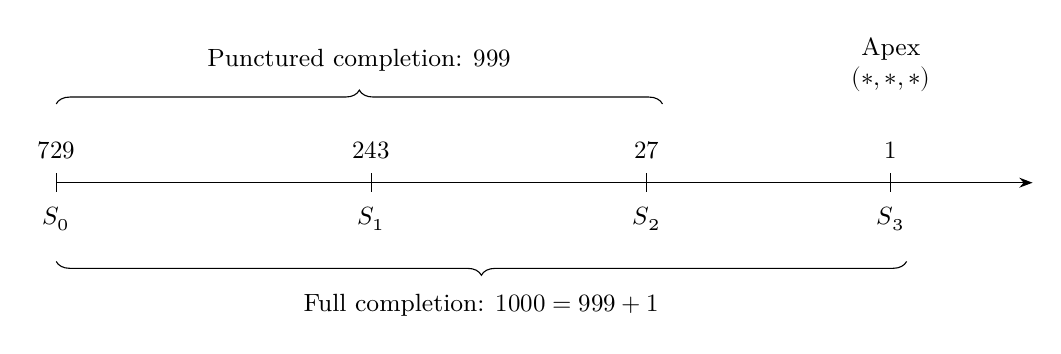
\begin{tikzpicture}[x=1cm,y=1cm,>=Stealth,font=\small]
\draw[->] (0,0)--(12.4,0);
\foreach \x/\a/\b in {0/729/{S_0},4.0/243/{S_1},7.5/27/{S_2},10.6/1/{S_3}}{
  \draw (\x,0.12)--(\x,-0.12);
  \node[above=5pt] at (\x,0) {\(\a\)};
  \node[below=5pt] at (\x,0) {\(\b\)};
}
\draw[decorate,decoration={brace,amplitude=5pt}] (0,1)--(7.7,1);
\node[above=8pt] at (3.85,1) {Punctured completion: \(999\)};
\draw[decorate,decoration={brace,mirror,amplitude=5pt}] (0,-1)--(10.8,-1);
\node[below=8pt] at (5.4,-1) {Full completion: \(1000=999+1\)};
\node[align=center] at (10.6,1.5) {Apex\\\((\ast,\ast,\ast)\)};
\end{tikzpicture}
\caption{Strata of the cubic completion. The arrangement represents
the set-theoretic decomposition, not a metric scale. The \(243\) elements
of \(S_1\) form three coordinate strata of \(81\) elements; the \(27\)
elements of \(S_2\) form three strata of \(9\). The apex completes the partition.}
\label{fig:revision-emrh}
\end{figure}

% Preserved historical vector figure; explanatory caption retained.
\begin{figure}[htbp]
\centering
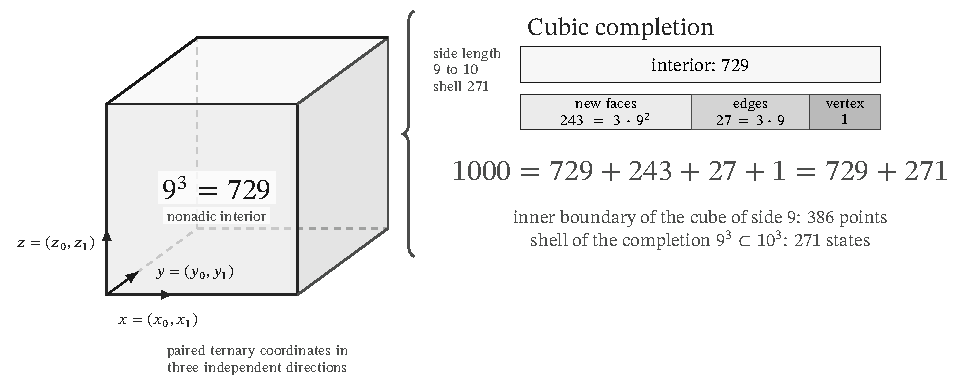
\includegraphics[width=\linewidth]{figures/cubo_emrh.pdf}
\caption{Cubic representation of the expansion from nine to ten classes per coordinate. Strata \(S_1,S_2,S_3\) locate the added incidences on faces, edges, and the apex; their cardinalities form the \(271\)-element shell. The \(386\)-element boundary belongs to the initial cube. This geometric perspective complements the partition in Figure~\ref{fig:revision-emrh}; graphical spacing is schematic.}
\label{fig:completacion-cubo-recuperado}
\end{figure}


\subsubsection{Conservation of unity and dimensional compatibility}

Normalization is not limited to dividing an isolated identity. In dimension
\(d\), the product \(\widehat E^d\) carries the uniform measure
\(\mu_d(\{x\})=10^{-d}\). The coordinate projection
\(p_d:\widehat E^{d+1}\to\widehat E^d\) deletes the last coordinate.

\Needspace{9\baselineskip}
\begin{samepage}
\begin{proposition}[Projective compatibility of normalized measures]
For every \(d\geq1\),
\[
 (p_d)_*\mu_{d+1}=\mu_d,
 \qquad \mu_d(\widehat E^d)=1.
\]
The mass of the stratum with \(r\) additional coordinates is
\(\binom dr9^{d-r}/10^d\), and the masses of all strata sum to one.
\end{proposition}
\end{samepage}
\begin{proof}
Each point of \(\widehat E^d\) has ten preimages. Their total mass is
\(10\,10^{-(d+1)}=10^{-d}\). Equality for any subset follows by
summing over its points. The stratified formula follows from the same
count as \eqref{eq:revision-estratos}; the binomial
\((9+1)^d\) gives total normalization.
\end{proof}

In dimension three, removing the apex leaves mass \(999/1000\), and
restoring it adds \(1/1000\). Renormalizing before restoration would
define a different measure: the distinction is operationally relevant.
In particular, conservation of probability mass, conservation of transport
records, and thermodynamic dissipation concern different objects. The
proposition proves the first and provides the compatible support for
studying the second; the third requires a specified dynamic and energetic realization.

The internal geometric boundary also remains distinct.
On the Cartesian representative \(\{1,\ldots,9\}^3\), removing
\(\{2,\ldots,8\}^3\) leaves \(386\) points. This boundary belongs
to the initial cube, whereas \(\widehat C\setminus C\) belongs to
its expansion. Cubic completion, base-thousand positional expansion,
and exceptional-incidence reading share support data; their respective
maps determine which information from these data each representation uses.


\subsection{Cubic incidence and Lorentzian realization}

Cubic completion supplies a relation between interior and boundary.
Its geometry can be developed through incidence of the six faces with
the eight vertices. Label faces by \((i,\varepsilon)\),
\(i\in\{1,2,3\}\), \(\varepsilon\in\{+1,-1\}\), and vertices by
\(\nu\in\{+1,-1\}^3\). The incidence matrix is
\[
 M_{(i,\varepsilon),\nu}=\mathbf1_{\{\nu_i=\varepsilon\}}.
\]
Let \(u=(1,\ldots,1)^{\mathsf T}\in\RR^6\), let \(R_F\) denote
face opposition, and let \(P_u=uu^{\mathsf T}/6\), \(P_-=(I-R_F)/2\).

\begin{proposition}[Four-dimensional incidence quotient]
The incidence Gram matrix satisfies
\[
 MM^{\mathsf T}=12P_u+4P_-.
\]
Its eigenvalues \(12,4,0\) have multiplicities \(1,3,2\).
Consequently,
\[
 Q_\square=\RR^6/\ker(MM^{\mathsf T})
 \simeq\RR u\oplus E_-,\qquad E_-=\operatorname{im}P_-.
\]
\end{proposition}
\begin{proof}
A face contains four vertices; two opposite faces have empty intersection,
and two distinct non-opposite faces share two vertices.
The matrix \(12P_u+4P_-\) has exactly these entries.
The uniform subspace has dimension one; differences between opposite
faces generate a three-dimensional space orthogonal to it.
Its complement has dimension two and belongs to the kernel.
\end{proof}

The decomposition \(1+3\) comes from incidence. The temporal choice
is declared through the bilinear form
\[
 B_\square([x],[y])=\langle x,(P_--P_u)y\rangle.
\]
It is well defined on the quotient because both projectors annihilate
the kernel. In the basis
\[
 t=[u]/\sqrt6,\qquad
 d_i=[e_{i,+}-e_{i,-}]/\sqrt2,
\]
its matrix is \(\operatorname{diag}(-1,1,1,1)\). The domain,
decomposition, and sign convention producing the Minkowski realization
are thus explicit. The positive Gram matrix determines the quotient;
the temporal assignment determines the indefinite form on it.

The operator
\[
 W_\square=\sqrt6P_u+\sqrt2P_-,\qquad
 W_\square e_{i,\varepsilon}=t+\varepsilon d_i
\]
sends the six face labels to null directions, since
\(B_\square(t+\varepsilon d_i,t+\varepsilon d_i)=-1+1=0\).
Direction reversal and face opposition thus acquire a concrete
geometric realization.

\subsubsection{Soldering, reversal, and subdivision}

The cellular realization uses an invertible transport \(U_m(a)\),
preserving the Lorentzian form, between the endpoint fibers of an
oriented dual edge \(a\), a face label \(\lambda_m(a)\),
and an orientation \(\sigma_m(a)\).
With \(\ell_m=\ell_0/9^m\), the soldering map is
\[
 \beta_m(a)=\ell_m\sigma_m(a)
 W_{\square,s(a)}e_{\lambda_m(a)}.
\]
Compatible reversal satisfies
\[
 \beta_m(\bar a)=-U_m(a)\beta_m(a).
\]
Identify the source fibers at two consecutive levels through the declared
refinement isometry. If the nine subsegments \(a_1,\ldots,a_9\),
at level \(m+1\), preserve label and orientation when transported
to that common fiber, then
\begin{equation}
 \beta_m(a)=\sum_{j=1}^9
 U_{m+1}(a_1\cdots a_{j-1})^{-1}\beta_{m+1}(a_j).
 \label{eq:soldadura-refinamiento}
\end{equation}
Each transported term equals \(\ell_m/9\) times the same null
direction, proving the identity. The compatibility hypothesis determines
which subdivisions realize this refinement. The equation brings together
direction, scale, and transport, rather than limiting geometric
correspondence to a dimension count.

With orientation and the Lorentzian form also fixed, Hodge duality
on \(\Lambda^2Q_\square^*\) satisfies \(\star^2=-I\).
In dimension four, the sign is \((-1)^{2(4-2)+1}=-1\).
This yields a real complex structure on two-forms and, after
complexification, the eigenspaces with eigenvalues \(+i\) and \(-i\).
The electromagnetic realization will use this domain after constructing
the electronic section and declaring its coupling.

\subsection{Compatibility of modular and positional reductions}

The block-decimal base enters through Euclidean division preserving
residue and quotient simultaneously:
\[
 n=1000q+r,\qquad 0\le r<1000.
\]
Since \(1000\equiv1\pmod9\) and \(1000\equiv1\pmod3\),
\[
 n\equiv q+r\pmod9,\qquad n\equiv q+r\pmod3.
\]
Reduction of a block therefore requires the quotient's contribution
to recover the integer's class. The numbers \(0\) and \(1000\)
have the same remainder modulo \(1000\), but different classes
modulo \(9\) and \(3\). This is an operational reason for preserving
memory through a change of resolution.

Ternary refinement and determination of a decimal prefix can be
coordinated through a single integer remainder. If \(N/3^L\)
is a cylinder endpoint and \(D/1000^r\) a decimal endpoint, define
\[
 A=1000^rN-D3^L.
\]
On adding six ternary symbols, \(N'=729N+\nu\),
\(L'=L+6\), with \(0\le\nu<729\). If the decimal prefix remains
fixed, one obtains
\[
 A'=729A+\nu1000^r.
\]
If a decimal block \(\delta\) is also incorporated, then
\(D'=1000D+\delta\), \(r'=r+1\), and
\begin{equation}
 A'=729000A+\nu1000^{r+1}-729\delta3^L.
 \label{eq:residuo-dos-bases}
\end{equation}
Both identities follow by substitution of the definitions. Comparing
endpoints is thus reduced to integer operations retaining each
prolongation's contribution. This compatibility makes it possible
to refine a region before evaluating its real coordinate.

% Incorporation at the end of extension.tex; contains no main section.
% Provenance: RESULTADO_RECUPERADO; sector-specific explicit statement of hypotheses.
% Sources read: Doble proyección holográfica monograph (editorial source material),
% manuscrito/local/01_tesis_recuperada.tex and
% manuscrito/generated/algebra_holonomica.tex, especially §§1--7 and 21.
% Governing definition of number: manuscrito/flattened/main_autosuficiente.tex,
% sections starting at lines 22137 and 23000 of the 775-page source collection.
% Its global presentation is not adopted as proof of every TPK arrow.

\subsection{Number as a compatible section and value as a reading}
\label{hist:seccion}

Distinguishing state from observation specifies what object is prolonged
as resolution increases. At depth \(n\), let \(X_n\) be the set of
admissible states produced by APP--TRIT--TPK. Their data include position,
sum and product sheets, residues and quotients, regime, orientation,
carry, phase, route, boundary, memory, and survival. These are not
independent coordinates: earlier arithmetic evaluations and transports
impose their relations. A prolongation preserves these relations in
each antecedent, even while adding new steps and memory data.
This is the meaning of the arithmetic of histories developed in
\cite{hmtintegral,hmtholonomia}.

Let \(r_{m,n}:X_m\to X_n\), for \(m\geq n\), be depth
restrictions, with \(r_{n,n}=\operatorname{id}\) and
\(r_{\ell,n}=r_{m,n}\circ r_{\ell,m}\). Each restriction preserves
the prefix and the information already determined in it.

\begin{definition}[Compatible numerical section]
An HMT number is a compatible history of the state system:
\begin{equation}
 x=(x_n)_{n\geq0}\in X_\infty:=\varprojlim_n X_n,
 \qquad r_{m,n}(x_m)=x_n.
 \label{hist:limite-inverso}
\end{equation}
A reader is an additional operation on a specified domain of these
histories. A digit is a finite observation; a scalar value is an evaluation
of the reader. The pair consisting of a section and its reader constitutes
a read presentation, not a redefinition of the section's identity.
\end{definition}

On the Archimedean domain \(X_\infty^{\mathrm{Arch}}\), the reader
associates a closed cylinder with each prefix, preserves nesting, and
makes its diameter tend to zero. It thus determines
\begin{equation}
 \operatorname{ev}_{\mathbb R}:X_\infty^{\mathrm{Arch}}\longrightarrow
 \mathbb R,\qquad
 \{\operatorname{ev}_{\mathbb R}(x)\}=\bigcap_n I_n(x).
 \label{hist:evaluacion}
\end{equation}
The concrete construction of these cylinders and the determination of
their boundaries are developed in Section~\ref{sec:generacion}.
Definition \eqref{hist:limite-inverso} does not by itself assert
that the image of \eqref{hist:evaluacion} is the entire line:
a coverage claim requires its own theorem. Nor does equality of
values establish equality of histories without an injectivity result.
This separation allows precision to be discussed as depth while preserving
the distinction between the arithmetic antecedent and its scalar realization.

\subsection{Composition of histories and memory multiplier}
\label{hist:algebra}

Fix a sector of states at depth \(n\) and a category \(\mathcal C\)
whose arrows are its admissible histories. Composition is written
\(vu=v\circ u\): first traverse \(u\), then \(v\).
Elementary steps come from TPK selection, transport, and updating.
A local tritic fiber admits the notation
\(\mathbb R[J_x]/(J_x^2+\tau(x)1_x)\), where
\(\tau(x)\in\{+1,0,-1\}\). Regime and orientation belong to
the transported state; a transition between regimes does not amount
to identifying their quadratic algebras.

The following formulation specifies an algebraic sector of this composition.
For each object \(x\), a unital associative real algebra \(A_x\),
possibly noncommutative, is given. For each \(u:x\to y\), a
unital homomorphism \(\rho_u:A_x\to A_y\) is given. Assume a strict action:
\begin{equation}
 \rho_{\operatorname{id}_x}=\operatorname{id}_{A_x},\qquad
 \rho_v\rho_u=\rho_{vu}.
 \label{hist:accion-estricta}
\end{equation}
For each composable pair \(u:x\to y\), \(v:y\to z\), fix an
invertible central multiplier \(\Omega(v,u)\in Z(A_z)^\times\).
Require the normalization
\(\Omega(\operatorname{id}_y,u)=\Omega(u,\operatorname{id}_x)=1_y\)
and, for every composable triple, the identity
\begin{equation}
 \rho_w\bigl(\Omega(v,u)\bigr)\Omega(w,vu)
   =\Omega(w,v)\Omega(wv,u).
 \label{hist:cociclo}
\end{equation}
These are explicit hypotheses on transports and their coefficients,
not a consequence of calling the dynamics holonomic. Applying this
presentation to a TPK sector requires identifying its \(\rho_u\)
and \(\Omega(v,u)\). Transitions expressed through bimodules require
preserving that structure and are not replaced by \eqref{hist:accion-estricta}.

The space of finite sums
\[
 \mathcal H(\mathcal C,A,\rho,\Omega)
   =\bigoplus_{u\in\operatorname{Mor}(\mathcal C)} A_{t(u)}T_u
\]
receives the bilinear product
\begin{equation}
 (aT_v)(bT_u)=a\rho_v(b)\Omega(v,u)T_{vu},
 \label{hist:producto}
\end{equation}
when the arrows are composable, and zero otherwise. Here \(t(u)\)
denotes the terminal state. Addition gathers histories with coefficients;
multiplication concatenates histories while preserving the record multiplier.

\begin{proposition}[Sectorial associativity with a central multiplier]
Under \eqref{hist:accion-estricta} and \eqref{hist:cociclo}, product
\eqref{hist:producto} is associative. If the object set is finite,
its identity is \(\sum_x1_xT_{\operatorname{id}_x}\).
\end{proposition}
\begin{proof}
For \(u:x\to y\), \(v:y\to z\), \(w:z\to t\), let
\(a\in A_y\), \(b\in A_z\), \(c\in A_t\). The two coefficients
of \(T_{wvu}\) are
\begin{align*}
 ((cT_w)(bT_v))(aT_u):\quad&
 c\rho_w(b)\Omega(w,v)\rho_{wv}(a)\Omega(wv,u),\\
 (cT_w)((bT_v)(aT_u)):\quad&
 c\rho_w(b)\rho_w\rho_v(a)\rho_w(\Omega(v,u))\Omega(w,vu).
\end{align*}
The strict action identifies \(\rho_w\rho_v(a)\) with \(\rho_{wv}(a)\).
Centrality of \(\Omega(w,v)\) allows it to move to the right of
that factor; \eqref{hist:cociclo} then equates the remaining products.
The coefficients \(a,b,c\) are not permuted. If the triple is not
composable, both parenthesizations are zero because of their initial
and terminal states. Bilinearity completes the proof. Local identities
and normalization of \(\Omega\) verify the stated identity element.
\end{proof}

Calendar carry provides an effective example. In the category with one
object and arrows \(C_9\), take coefficients
\(A=\mathbb R[z,z^{-1}]\), the identity action, and
\[
 \Omega(b,a)=z^{c_0(a,b)},\qquad
 c_0(a,b)=\left\lfloor\frac{a+b}{9}\right\rfloor,
 \quad 0\leq a,b<9.
\]
The two carry sums of a triple are
\(\lfloor(a+b+c)/9\rfloor\); hence \eqref{hist:cociclo} holds.
The formal variable \(z\) records the turn without assigning it a
numerical value. Subsequently imposing \(z^{12}=1\) recovers the
dodecaphase record of calendar \eqref{eq:extension108}; retaining
\(z\) without that relation distinguishes successive turns. The example
realizes this calendar's memory without identifying it with all TPK memory.

\subsection{Double variance of refinement and conservation of unity}
\label{hist:doble-varianza}

Restricting states prolongs observables in the opposite direction.
Consider the function algebras, with pointwise product,
\(D_n=\operatorname{Fun}(X_n,\mathbb R)\). Precomposition defines
\begin{equation}
 r_{m,n}^*:D_n\longrightarrow D_m,
 \qquad r_{m,n}^*f=f\circ r_{m,n}.
 \label{hist:precomposicion}
\end{equation}
These are unital morphisms; they are also injective when the corresponding
restrictions are surjective. The direct limit
\(D_{\mathrm{cyl}}=\varinjlim_n(D_n,r_{n+1,n}^*)\) gathers
finite-depth observations. This algebra is not identified here with
the whole route algebra: prolonging transport operators also requires
their compatibility with refinement.

\begin{lemma}[Identity and naturality of evaluation]
If \(e_x\) is the indicator of \(x\in X_n\), then
\begin{equation}
 r_{m,n}^*e_x=\sum_{y:\,r_{m,n}(y)=x}e_y,
 \qquad r_{m,n}^*1_n=1_m,
 \label{hist:unidad}
\end{equation}
and, for every \(f\in D_n\), \(y\in X_m\),
\[
 \langle r_{m,n}^*f,y\rangle=\langle f,r_{m,n}y\rangle.
\]
Each section \(x\in X_\infty\) determines a well-defined evaluation
\(D_{\mathrm{cyl}}\to\mathbb R\), given by \([f]\mapsto f(x_n)\)
for \(f\in D_n\).
\end{lemma}
\begin{proof}
The fibers of \(r_{m,n}\) partition \(X_m\). Their indicators
are orthogonal and sum to \(1_m\), proving \eqref{hist:unidad}.
Naturality is the definition of precomposition. Finally,
\((r_{m,n}^*f)(x_m)=f(x_n)\), so two compatible representatives
give the same evaluation in the direct limit.
\end{proof}

The global identity is the constant function one on all possibilities;
an individual section selects a compatible history. Preserving the former
does not mean immobilizing the latter. Refinement may increase the number
of extensions and the depth of each history while preserving the identity
and all evaluations of its antecedents.

\subsection{Phase return, Weyl representation, and two readings}
\label{hist:puente-lecturas}

Law \eqref{eq:holonomia-memoria} acquires an operator realization
in the bilateral suspension constructed in Section~\ref{sec:generacion}.
There, \(T\) is one-step advance, \(V_9\) observes the nonadic phase,
\(W_\delta\) the rotation phase, and \(D_M\) the memory degree.
Writing \(\widehat\Gamma_9=T^9\) for the turn in this representation,
the Weyl relations \eqref{eq:weyl-relojes} imply, on finitely
supported vectors,
\begin{equation}
 \begin{aligned}
 V_9\widehat\Gamma_9&=\widehat\Gamma_9V_9,\qquad
 W_\delta\widehat\Gamma_9=e^{2\pi i9\delta}
     \widehat\Gamma_9W_\delta,\\
 [D_M,\widehat\Gamma_9]&=\widehat\Gamma_9.
 \end{aligned}
 \label{hist:tres-retornos}
\end{equation}
The first equality follows from \(\zeta_9^9=1\); the second from
nine applications of the covariance of \(W_\delta\); the third
expresses the unit memory increment. The finite phase returns while
irrational rotation and memory distinguish the next state. Characters
and parameter \(\delta\) are realized subsequently from the numerical
construction specified there: they do not select the seeds retrospectively.
This representation describes suspension observables and translations;
it does not replace all TPK coordinates or operators.

The double reading extends the same distinction between history and observable.
On its Archimedean domain, \eqref{hist:evaluacion} applies; on the
calibrated incidence domain, the maps \(Q_n\) of
Section~\ref{exc:doble-lectura} preserve words and boundary frames.
The equality proved there,
\(r_{n,m}Q_n=Q_mp_{n,m}\), determines their prolongation \(Q_\infty\).
On the common domain of both readings,
\(\operatorname{ev}_{\mathbb R}(x)\) and \(Q_\infty(x)\)
can be considered jointly: the former retains the value; the latter,
the transported incidence preserved by its codomain. The section
precedes both. This articulation makes it possible to pass from the
arithmetic of histories to constants and exceptional reading without
turning their realizations into new initial data.


\clearpage\section{Coinductive generation of \texorpdfstring{\(\pi,\varphi,e\)}{pi, phi, e} to arbitrary depth}
\label{sec:generacion}

The six-block emission is a finite stage of the construction, not a complete decimal expansion. Its function is to produce regions with multiplicity, orientation, and transport rules. Prolongation must preserve these data and determine a compatible collection of prefixes of arbitrary length. The word \emph{generation} designates this operation; \emph{genealogy} designates the reconstruction of its dependencies. Both notions enter the account, but serve different functions.

\subsection{Orbits, regions, and characters of closure, propagation, and self-scaling}

On a word \(w=(w_1,\ldots,w_6)\), define
\[
 r(w)=(w_3,w_1,w_2,w_5,w_6,w_4),\qquad
 s(w)=(w_4,w_5,w_6,w_1,w_2,w_3).
\]
We have \(r^3=s^2=I\) and \(srs=r^{-1}\); hence these permutations realize the dihedral group \(D_3\). The action preserves the catalog and multiplicities and commutes with \(\Psi\). The quotient of the \(243\) visible words has \(43\) orbits: thirty-eight of cardinality six and five of cardinality three.

The closure class is recognized by a fiber predicate: its six orientations have five emissions per word, total multiplicity \(1008\), and distribution \(432+4\cdot144\). There is a single orbit with these properties in the catalog. To specify the other two selections, write \(f(w)=\#\Psi^{-1}(w)\), \(m(w)=\sum_{U\in\Psi^{-1}(w)}\operatorname{mult}(U)\), and \(\nu(w)=(n_0,n_1,n_2)\). The additive diagonal class of an emission is \(d(U)=[i+j]_9\) in indices from zero to eight; its additive signature preserves this class and the \(ES\) or \(NO\) orientation. Let \(\mathcal D(\mathcal O)\) be the set of these classes for all emissions over an orbit.

Among the size-six orbits, the joint predicate
\[
 f(w)=1,\qquad m(w)=144\quad(w\in\mathcal O),\qquad
 \mathcal D(\mathcal O)=\{0,3,6\}
\]
leaves exactly six orbits. In this sector, the census \(\nu=(2,3,1)\), equal to that of closure, uniquely selects propagation; the census \(\nu=(2,2,2)\) uniquely selects self-scaling. The diagonal support cannot be omitted: without it there are four balanced singleton-fiber orbits of multiplicity \(144\), not one. Finally, the existence of an emission with \(d=6\) and orientation \(ES\) selects one representative of each orbit and yields
\begin{equation}
 w^{\rm cl}=010211,\qquad w^{\rm pr}=201101,\qquad w^{\rm au}=121200.
 \label{eq:palabras-regionales}
\end{equation}
These symbols first designate regions of the catalog. The scalar identification will be proved through their readers; they are not chosen because they match digits of a known constant.

The closure word \(010211\) has the following five preimages:
\begin{center}\small
\begin{tabular}{@{}lll r@{}}\toprule
Six-block emission&Multiplicative signature&Role&Multiplicity\\\midrule
\(501,614,498,169,272,272\)&\(555555\)&transverse&432\\
\(810,923,870,169,272,272\)&\(339555\)&positive orientation&144\\
\(810,983,810,169,272,272\)&\(393555\)&positive orientation&144\\
\(870,923,810,169,272,272\)&\(933555\)&positive orientation&144\\
\(870,923,810,418,674,521\)&\(933717\)&oriented return&144\\\bottomrule
\end{tabular}
\end{center}
The multiplicity \(432\) and constant signature \(555555\) characterize the transverse region. They do not identify the central position \((5,5)\) of APP. Confusing a six-window signature with a position in the support would eliminate the distinction between numerical region and electronic structure.

The microfiber also has a precise bipartite morphology. Each emission is a product of an additive cursor class and a multiplicative class. The three positive regions share the same additive class of eighteen conditions; together they contain three multiplicative classes of eight conditions each. The transverse region has a product \(18\times24\); the three positive regions together have another \(18\times24\); and the return has a product \(18\times8\). The decomposition by emissions has five parts, whereas the decomposition by connected components of the bipartite graph has three. Both preserve the same \(1008\) seeds without reducing form to a cardinality.

\subsection{Finite transport and the prolongation boundary}

The endomorphisms \(L_0,L_1\) of the ternary-word space act before the Archimedean realization. Their determination begins with the transitions of the arithmetic state, not with the prescription of two matrices. If \(U_t\) is the composite selection, transport, and update step, the observed block satisfies
\[
 b_j^\chi=\Pi_6(x_j^\chi),\qquad
 x_{j+1}^\chi=U_{9j+9}\cdots U_{9j+1}(x_j^\chi),
 \qquad \chi\in\{\mathrm{cl},\mathrm{pr},\mathrm{au}\}.
\]
Six transitions are formed for each regime: two consecutive transitions in each of the three regions. The pairs of source and target matrices obtained in the record are
\[
\begin{array}{c|c|c|c}
X_0&Y_0&X_1&Y_1\\\hline
010211&012222&010211&002111\\
012222&010211&002111&110221\\
201101&121221&102011&012222\\
121221&102011&012222&102011\\
121200&112202&121020&010210\\
112202&121020&010210&010200
\end{array}
\]
Each six-digit string represents a row in \(\FF_3^6\). Since \(\det X_0=1\) and \(\det X_1=-1\) in \(\FF_3\), the equations \(X_aL_a=Y_a\) uniquely determine \(L_a=X_a^{-1}Y_a\). In this row-vector chart, the resulting matrices are
\[
 L_0=\begin{pmatrix}
 2&2&2&1&2&1\\2&1&2&2&1&1\\1&0&0&1&0&2\\
 0&0&1&1&1&0\\2&2&2&0&2&1\\2&1&2&1&0&0
 \end{pmatrix},\quad
 L_1=\begin{pmatrix}
 2&1&2&0&2&2\\1&2&1&1&2&0\\1&2&1&1&1&2\\
 0&1&0&0&2&1\\2&0&2&1&0&1\\0&2&2&2&1&1
 \end{pmatrix}\quad(\bmod3).
\]
The calendar \((L_0,L_0,L_1,L_1)\) produces four new six-component blocks. Their concatenations form
\[
 w_6\longrightarrow w_{12}\longrightarrow w_{18}
 \longrightarrow w_{24}\longrightarrow w_{30}.
\]
The subscripts of \(w\) indicate accumulated length. The boundary \(R_{36}\) preserves the terminal structure and opens the prolongation relation; it is not renamed as a final periodic block that could be repeated indefinitely.

The identity \(L=X^{-1}Y\) proves uniqueness once the transitions are fixed; it does not replace the production of those transitions by \(U_t\). The provenance of their record and the examination of the sixteen binary calendars are documented in the technical supplement. The indicated calendar is the only one of those sixteen that jointly reproduces the three five-block sequences.

\subsection{Five closure regions and angular compensation}

The closure region contains a transverse component and four accompanying components. The symmetric reader acts on the space of its five positions through
\[
 P_5=\frac15\mathbf1\mathbf1^{\mathsf T},\qquad
 \mathbf1=(1,1,1,1,1)^{\mathsf T}.
\]
The invariance \(P_5\lambda=\lambda\) and conservation \(\mathbf1^{\mathsf T}\lambda=1\) force \(\lambda=\mathbf1/5\). This normalization distributes the unit among reader positions; it does not replace the seed multiplicities \(432,144,144,144,144\) with uniform frequencies. The reader's elliptic chart realizes each coordinate through \(1+\lambda_jJ\); its slope is \(\lambda_j\), so the primitive slope is \(1/5\). This makes explicit the rule passing from a normalized coordinate to a slope, rather than identifying the two notions without a map. The reader composes the four accompanying positions through the law
\begin{equation}
 a\oplus b=\frac{a+b}{1-ab}.
 \label{eq:suma-pendientes}
\end{equation}
This law is obtained by multiplying \((1+aJ)(1+bJ)\) in the regime \(J^2=-I\) and dividing by its scalar component. The composition of slopes is therefore a realization of the quadratic structure of TRIT, not an ordinary sum of four fractions.

\begin{proposition}[Closure compensator]
The composition of four slopes \(1/5\) is \(120/119\). The condition of return to slope one determines a unique positive compensator of the form \(1/q\), with \(q>1\), and gives \(q=239\).
\end{proposition}
\begin{proof}
The first doubling gives \((1/5)\oplus(1/5)=5/12\); the second gives \((5/12)\oplus(5/12)=120/119\). The condition
\[
 \frac{120/119-1/q}{1+(120/119)/q}=1
\]
is equivalent to \((120-119)q=120+119\), so \(q=239\).
\end{proof}

The resulting closure character has realization
\begin{equation}
 \Pi_{\rm cl}=4\left(4\arctan\frac15-\arctan\frac1{239}\right).
 \label{eq:lector-pi}
\end{equation}
Machin's angular identity recognizes \(\Pi_{\rm cl}=\pi\). The meaning of the construction is precise: the slope and number of compositions are declared by the pentafiber reader; the compensation equation forces \(239\). Once this character has been produced, its evaluation through alternating series does not select the seed orbit anew.

For \(0<x<1\), the alternating sums
\[
 A_n(x)=\sum_{j=0}^n\frac{(-1)^jx^{2j+1}}{2j+1}
\]
enclose \(\arctan x\) between two consecutive truncations, with difference \(x^{2n+3}/(2n+3)\). Applied to the two slopes in \eqref{eq:lector-pi}, they provide rational endpoints with explicit error. The numerical value is thus computed as a consequence of the exact character, without introducing a target prefix.

\subsection{Propagation reader and normalization of the unit}

The propagation region is realized through a formal collection \(P_t\in\mathcal A[[t]]\), where \(\mathcal A\) is a unital commutative algebra over \(\QQ\). Its composition satisfies \(P_{t+s}=P_tP_s\), with unit \(P_0=1\), and the oriented elementary transport fixes the scalar generator \(P'_0=+1\). The condition fixes its sign, not merely its magnitude. Writing
\[
 P_t=\sum_{n\ge0}a_nt^n,
\]
the normalization determines \(a_0=a_1=1\). Comparing the coefficient of \(s^nt\) in \(P_{s+t}=P_sP_t\) gives \((n+1)a_{n+1}=a_na_1\); equivalently, \(P'_t=P_t\). Thus,
\begin{equation}
 (n+1)a_{n+1}=a_n,\qquad a_n=\frac1{n!}.
 \label{eq:propagacion}
\end{equation}
The character at one parameter unit is \(\Pi_{\rm pr}=P_1\), subsequently recognized as \(e\).

The normalization of the generator matters. Without this datum, the semigroup law would admit \(P_t=e^{ct}\) for different \(c\); the condition fixing the parameter unit in the reader is therefore not omitted. This condition precedes the decimal comparison and belongs to the exposition of the operational rule, not to the choice of an experimental value.

\begin{proposition}[Rational propagation bounds]
For \(n\ge1\), let \(E_n=\sum_{j=0}^n1/j!\). Then
\[
 E_n<\Pi_{\rm pr}<E_n+\frac{n+2}{(n+1)(n+1)!}.
\]
\end{proposition}
\begin{proof}
The first omitted term is \(1/(n+1)!\). Each subsequent ratio is at most \(1/(n+2)\). The geometric majorant of the tail is
\[
 \frac1{(n+1)!}\frac1{1-1/(n+2)}
 =\frac{n+2}{(n+1)(n+1)!}.
\]
The strict inequality follows from the decrease in successive ratios.
\end{proof}

\subsection{Modal incidence and generation of self-scaling}

The tritic selector produces the cycle \((+1,-1,0)\). In modes \(\Sigma,\Pi\), the rule is \(+1:m\mapsto\Sigma\), \(-1:m\mapsto\Pi\), \(0:m\mapsto m\). With cyclic closure, the observed mode is \((\Sigma,\Pi,\Pi)\). Its edges are \(\Sigma\to\Pi\), \(\Pi\to\Pi\), and \(\Pi\to\Sigma\). Hence its incidence, in that order of modes, is
\begin{equation}
 F_{\rm av}=\begin{pmatrix}0&1\\1&1\end{pmatrix}.
 \label{eq:fav}
\end{equation}
The four entries are obtained from the calendar, not from an equation previously supplied with the value of \(\varphi\). Repeating the calendar gives counts \(3F_{\rm av},9F_{\rm av},36F_{\rm av}\) at lengths nine, twenty-seven, and one hundred eight. These counts are not powers of the matrix.

\begin{theorem}[Positive self-scaling character]
The incidence \eqref{eq:fav} has a unique strictly positive eigenray. Normalizing it as \((1,x)^{\mathsf T}\), its coordinate \(x\) satisfies \(x^2-x-1=0\), \(x>0\), and equals \(\varphi=(1+\sqrt5)/2\).
\end{theorem}
\begin{proof}
The eigenvalue equation gives \(x=\lambda\) and \(1+x=\lambda x\). Eliminating \(\lambda\) produces the polynomial. Only one of its two roots is positive. Since \(F_{\rm av}^2\) has all entries positive, the positive ray is unique and simple. The radical expression recognizes the coordinate obtained; it does not participate in producing \(F_{\rm av}\).
\end{proof}

With \(F_0=0,F_1=1,F_{n+1}=F_n+F_{n-1}\), the incidence induces, for \(n\geq1\),
\[
 F_{\rm av}^n=\begin{pmatrix}F_{n-1}&F_n\\F_n&F_{n+1}\end{pmatrix}.
\]
The consecutive ratios \(F_{n+1}/F_n\) alternate around \(\varphi\). The determinant identity
\[
 F_{n+1}^2-F_nF_{n+2}=(-1)^n
\]
gives an exact width \(1/(F_nF_{n+1})\) between two consecutive ratios. Their growth makes this rational bracket arbitrarily narrow.

The measure on all compatible histories does not coincide with the frequency of modes in the three-event calendar. The chronological frequency is \((1/3,2/3)\). The maximal-entropy measure of the symbolic envelope defined by \(F_{\rm av}\) is constructed from its eigenvectors and has weight ratio \(\varphi^{-2}\). The latter enters the areal--volumetric reading; it is not obtained simply by replacing one counting frequency with another.

After the characters have been generated, the two orientations of the reader
\[
 R(x,y)=\frac{x}{y^2}
\]
provide
\begin{equation}
 \rho_A=\frac\pi{\varphi^2},\qquad
 \rho_E=\frac\varphi{\pi^2},\qquad
 \varphi^3\rho_A^2\rho_E=1.
 \label{eq:areal-electron}
\end{equation}
The second expression will appear in the electronic exponent. The first is also obtained as the limit of the marked reading \(\pi F_{n-1}/F_{n+1}\). Exchanging the arguments relates the two, but does not turn a reparameterization of the electronic equation into a second independent derivation of all its coefficients.

% Articulation subsequent to generation of pi, phi, and e.
% Cumulative content; does not replace the preceding TRIT development.
\subsection{Exponential realizations of the generated coordinates}
\label{euler-trit-articulacion}

The regional coordinates already determined allow recognition of concrete
realizations of the TRIT quadratic collection. The order is substantive:
construction of the regions precedes evaluation of an exponential at
parameters \(\pi\) or \(2\log\varphi\). These expressions identify
the role of the coordinates in operators constructed from APP and TPK;
they do not participate in selecting the prefixes that produce them.

\subsubsection{Ternary cycle, nilpotent transport, and sheet incidence}

Multiplication \(a(r)=4r\) in \(\mathbb Z/9\mathbb Z\) has order
\(3\). On the units it determines the orbits \(\{1,4,7\}\) and
\(\{2,8,5\}\). In the augmentation module of either orbit, consisting
of integer combinations whose coefficients sum to zero, the basis
\((e_r-e_{4r},e_{4r}-e_{7r})\) gives
\[
 C=\begin{pmatrix}0&-1\\1&-1\end{pmatrix},
 \qquad C^2+C+I=0.
\]
The restricted form has Gram matrix
\(\bigl(\begin{smallmatrix}2&-1\\-1&2\end{smallmatrix}\bigr)\).
On residue evaluations modulo \(9\), the action distinguishes the sheets:
\(S(ax,ay)=aS(x,y)\), whereas \(P(ax,ay)=a^{-1}P(x,y)\).
The cyclic realization therefore preserves a contragredient orientation
between sum and product. Quotients of the integer lift are retained
in the corresponding arithmetic record.

Elementary parabolic transport is represented by
\[
 N=\begin{pmatrix}0&1\\0&0\end{pmatrix}.
\]
The areal--volumetric incidence already constructed in \eqref{eq:fav} gives
\[
 F_{\rm av}=\begin{pmatrix}0&1\\1&1\end{pmatrix},
 \qquad A=F_{\rm av}^2=\begin{pmatrix}1&1\\1&2\end{pmatrix}.
\]
The three operators act on declared real spaces: the augmentation module
tensored with \(\mathbb R\), the nilpotent-transport plane, and the
modal-incidence plane. Sharing a matrix dimension does not identify
these spaces or their coordinates.

\begin{proposition}[Concrete generators of the three types]
\label{euler-trit-generadores}
The operators
\[
 J_{\mathrm e}=\frac{2C+I}{\sqrt3},\qquad
 J_{\mathrm p}=N,\qquad
 J_{\mathrm h}=\frac{2A-3I}{\sqrt5}
\]
satisfy, respectively,
\[
 J_{\mathrm e}^{\,2}=-I,\qquad
 J_{\mathrm p}^{\,2}=0,\qquad
 J_{\mathrm h}^{\,2}=I.
\]
\end{proposition}
\begin{proof}
The relation for \(C\) implies \((2C+I)^2=-3I\).
Direct multiplication gives \(N^2=0\).
Finally, \(A\) has trace \(3\) and determinant \(1\), so
\(A^2-3A+I=0\) and \((2A-3I)^2=5I\).
\end{proof}

\begin{proposition}[Three evaluations of the exponential identity]
\label{euler-trit-evaluaciones}
In the preceding realizations,
\begin{equation}
 \boxed{
 \exp(\pi J_{\mathrm e})+I=0,\qquad
 \exp(J_{\mathrm p})=I+J_{\mathrm p},\qquad
 \exp(2\log\varphi\,J_{\mathrm h})=F_{\rm av}^{\,2}.}
 \label{euler-trit-tres-evaluaciones}
\end{equation}
\end{proposition}
\begin{proof}
The elliptic specialization of the tritic exponential gives
\(\cos\pi\,I+\sin\pi\,J_{\mathrm e}=-I\).
Nilpotency removes exactly the terms of degree at least \(2\)
in the second expression. For the third, \(\varphi^2=\varphi+1\) implies
\[
 \cosh(2\log\varphi)=\frac32,\qquad
 \sinh(2\log\varphi)=\frac{\sqrt5}{2}.
\]
Thus the exponential equals
\(\frac32I+\frac{\sqrt5}{2}J_{\mathrm h}=A\).
\end{proof}

The first equality represents the elliptic half-turn; the complete turn
satisfies \(\exp(2\pi J_{\mathrm e})=I\). The second retains a
nonzero linear term: the parabolic regime expresses transport, not absence
of evolution. The third realizes a unimodular hyperbolic advance. Its
eigenvalues are \(\varphi^2\) and \(\varphi^{-2}\); one direction
expands and the other contracts while preserving the determinant. The
three evaluations use different parameters of one common exponential collection.

In this collection, \(e\) enters through the scalar evaluation
\(\exp(I)=eI\) and the law \(\exp(sI)\exp(tI)=\exp((s+t)I)\).
Its role is not restricted to the parabolic type. The coordinate \(e\),
previously obtained from its region, is recognized here as the unit
evaluation of the exponential; this identity does not replace its
coinductive genealogy.

\subsubsection{Polynomial resolution of the regimes}

The three realizations admit a compact presentation on the direct sum
of their spaces. Define
\[
 \mathbb J=J_{\mathrm e}\oplus J_{\mathrm p}\oplus J_{\mathrm h},
 \qquad Q=\mathbb J^2.
\]
The preceding relations imply
\[
 \mathbb J^6=\mathbb J^2,\qquad Q^3=Q.
\]
Using \(Q\) keeps this operator square distinct from the
dodecaphase record \(K\).

\begin{proposition}[Polynomial regime projectors]
\label{euler-trit-proyectores}
The maps
\[
 p_{\mathrm e}=\frac{Q^2-Q}{2},\qquad
 p_{\mathrm p}=I-Q^2,\qquad
 p_{\mathrm h}=\frac{Q^2+Q}{2}
\]
are mutually orthogonal idempotents, sum to \(I\), and recover
the three summands of the representation.
\end{proposition}
\begin{proof}
The three polynomials take values \((1,0,0)\), \((0,1,0)\), and
\((0,0,1)\) at the points \(-1,0,+1\), respectively. The differences
between their squares and themselves, as well as their cross products,
are multiples of \(X^3-X\). Substituting \(Q\), which annihilates
that polynomial, proves the identities. On the three blocks, \(Q\)
acts as \(-I,0,I\).
\end{proof}

One thus obtains
\begin{align}
 \exp(t\mathbb J)
 ={}&p_{\mathrm e}(\cos t\,I+\sin t\,\mathbb J)
   +p_{\mathrm p}(I+t\mathbb J)\notag\\
   &+p_{\mathrm h}(\cosh t\,I+\sinh t\,\mathbb J).
 \label{euler-trit-exponencial-total}
\end{align}
Each summand preserves its quadratic relation, and conjugation reverses
its evolution. The total representation gathers the three regimes, but
does not by itself define a transition operator between them. Such a
transition requires the TPK transport maps with their domains, orientation,
and memory. The exponential articulation allows recognition of their
types without replacing those dynamics by an identification of fibers.

% FOCAL PROVENANCE (not printed)
% Recovered result: three generators and three exponential evaluations.
% Complete source owner:
% BASE/manuscrito/sections/hmt/09b_algebras_cuadraticas.tex:289-516.
% Causal antecedent of C and contragredient action:
% BASE/manuscrito/sections/hmt/03d_esqueleto_ciclotomico_app.tex:13-47,145-246.
% The three types and orientation are in:
% BASE/manuscrito/sections/hmt/02_trit_geometrias.tex:83-196.
% Recovered polynomial resolution:
% output/INVESTIGACION_HOLONOMIA_NONADICA_CRISTAL_APERIODICO_20260903/
% ALGEBRA_HOLONOMICA_UNIVERSAL_Y_EULER_TRITICO.md, sections 8-11 and 22.
% All four source owners were read fully. BASE denotes:
% /Users/ruben/Documents/HMT2/
% EL_CIERRE_HOLOGRAFICO_DEL_INFINITO_SUCESOR_102_CAPITULOS_2026-08-28_EN_TRABAJO/
% The identity P9(alpha)=delta from the specialized document is not incorporated:
% that identification does not belong to this block.
% Nor is a nilpotent direction identified with electronic vacancy,
% or a global transport representation by the direct sum presumed.
% CHECKS: standard Python, integers, and Fraction.
% C^2+C+I=0; (2C+I)^2=-3I; N^2=0; (2Fav^2-3I)^2=5I.
% 81 residue pairs verify the two contragredient actions.
% The 3 projectors were checked at Q=-1,0,+1; general proof in the text.
% 6 unique labels and balanced environments. No compilation.


\subsection{Compatible cylinders and arbitrary depth}

The realization of a ternary block \(b=(b_1,\ldots,b_6)\) is the integer
\[
 \nu(b)=\sum_{j=1}^6b_j3^{6-j}\in\{0,\ldots,728\}.
\]
A block sequence defines integer prefixes through \(N_{n+1}=729N_n+\nu(b_{n+1})\), starting at \(N_0=m\), where \(m\) is the integer part determined by the reader. The preceding brackets place the closure, propagation, and self-scaling characters in \((3,4)\), \((2,3)\), and \((1,2)\), respectively; hence their initial values are \(m=3,2,1\). The following blocks refine the fractional part. The corresponding cylinder is
\begin{equation}
 I_n=\left[\frac{N_n}{729^n},\frac{N_n+1}{729^n}\right],
 \qquad |I_n|=729^{-n}.
 \label{eq:cilindro}
\end{equation}
The half-open convention is used to select a representative when a value lies on a boundary. For passage to the limit, the closures of these intervals are used, and the two equivalent boundary expansions are identified. This qualification prevents the assumption that every intersection of nested half-open intervals is automatically nonempty.

\begin{theorem}[Determination of the scalar realization]
A compatible block history determines a unique limit of the left endpoints of \eqref{eq:cilindro}. If an exact character has rational brackets of arbitrarily small width and is separated from the boundary of every decimal cylinder examined, each decimal prefix of finite length is determined after a finite computation. The prefixes thus obtained are mutually compatible.
\end{theorem}
\begin{proof}
Extending by one block preserves the preceding prefix through Euclidean division. The closed cylinders are nested and their diameter tends to zero; their left endpoints are Cauchy and have a unique limit. For a fixed decimal length, a value separated from the partition boundaries has positive distance from them. A sufficiently narrow bracket lies within a unique cell and determines its prefix. Uniqueness of the cell and nesting of the partitions prove compatibility under truncation. At points with a terminating expansion, the exact boundary decision and its representation convention must be added; that decision does not follow from numerical width alone.
\end{proof}

The closure, propagation, and self-scaling characters have the preceding brackets. After their recognition, the irrationality of \(\pi,e,\varphi\) guarantees their separation from the rational boundaries at any finite decimal precision. Arbitrary depth means \emph{for every finite horizon there exists a computation determining its prefix}; it does not require a finite machine to store infinitely many digits at once. The mathematical object is the full compatible collection, and an execution produces a finite projection of it.

\subsection{Specular involution and synchronization of the regions}

The nonadic connection jointly transports the three characters. In the ninth-phase chart, the self-scaling axis and the ternary sum of closure and propagation remain fixed under the specular exchange. Helical inversion changes the direction of transport; the mirror of the two channels changes their relative orientation. These are different involutions, although both act on the same trajectory system.

The census coincidences illustrate this coordination:
\begin{center}
\begin{tabular}{@{}c rrr l@{}}\toprule
Phase&\(N_\pi\)&\(N_e\)&\(N_\varphi\)&Equality of counts\\\midrule
4&207&207&122&\(N_\pi=N_e\)\\
5&39&151&151&\(N_e=N_\varphi\)\\
6&110&110&69&\(N_\pi=N_e\)\\
7&81&29&81&\(N_\varphi=N_\pi\)\\
8&59&59&59&triple synchronization\\
9&43&43&43&triple synchronization\\\bottomrule
\end{tabular}
\end{center}
These integers count compatible coordinates of the regions. They do not assert equality of \(\pi\), \(e\), and \(\varphi\) as real numbers. If
\[
 \partial(a,b,c)=(a-b,b-c,c-a),
\]
its image belongs to the lattice \(A_2=\{(u,v,w)\in\ZZ^3:u+v+w=0\}\). In phases eight and nine, the relative component vanishes, but the diagonal component changes from \((59,59,59)\) to \((43,43,43)\). Relative synchronization coexists with a displacement of \(-16\) per channel. The closure leading to \(\alpha\) must preserve both pieces of information: relative agreement and the evolution of memory.

\subsection{Sturmian helical suspension}

The relation between bases nine and ten in the completion defines the dimensionless parameter
\begin{equation}
 \delta=\frac{\log(10/9)}{\log10}.
 \label{eq:delta-sturm}
\end{equation}
It is not obtained from a target physical constant. It is the relative logarithmic scale of two bases already present in the construction. Its use as a symbolic reading of refinement has an exact consequence.

\begin{lemma}[Irrationality of the slope]
The number \(\delta\) is irrational.
\end{lemma}
\begin{proof}
If \(\delta=p/q\), \(q>0\), then \((10/9)^q=10^p\) and \(9^q=10^{q-p}\). The factorization of the left-hand side contains the prime three, whereas that of the right-hand side contains only the primes two and five. Equality is impossible.
\end{proof}

The lower mechanical word, with intercept \(\theta\), is
\[
 z_n(\theta)=\lfloor(n+1)\delta+\theta\rfloor-\lfloor n\delta+\theta\rfloor\in\{0,1\}.
\]
It is obtained by observing the rotation \(\theta\mapsto\theta+\delta\pmod1\) through the interval \([1-\delta,1)\). The event sequence has density \(\delta\), and its sum over any window of length \(L\) equals \(\lfloor L\delta\rfloor\) or \(\lceil L\delta\rceil\). Since \(21<1/\delta<22\), event separations are twenty-one or twenty-two. The word indicating which intervals are short is another mechanical word of slope \(\sigma=22-1/\delta\); its events are separated by six or seven primary intervals. The second scale is induced by the first, not a second free parameter.

% Reunited development from DESARROLLO_MATEMATICO, sections 38--40 and 50.
\subsubsection{Capacity index, vacancies, and induction of the tritic regime}
\label{vac-capacidad-trit}

The vacancy sequence is linked to refinement through an increment identity.
To exhibit it, fix the phase origin \(\theta=0\). Let
\[
 \rho=\log_{10}9=1-\delta,\qquad
 \mathcal C_t=\lfloor(t+1)\rho\rfloor\quad(t\geq0).
\]
The index \(\mathcal C_t\) expresses the decimal capacity of refinement
in the normalization comparing a ternary block of \(6\) positions,
with \(729\) possibilities, and a decimal block of \(3\) positions,
with \(1000\) possibilities. Indeed,
\(\log_{1000}729=\log_{10}9=\rho\). The letter \(K\) is reserved
for the dodecaphase record constructed later.

\begin{proposition}[Complementarity of capacity and vacancy]
\label{prop:capacidad-vacancia}
For \(t\geq1\),
\begin{equation}
 \mathcal C_t-\mathcal C_{t-1}=1-z_t(0).
 \label{eq:capacidad-vacancia}
\end{equation}
Consequently, if \(0\leq a<b\),
\[
 \mathcal C_b-\mathcal C_a+
 \sum_{t=a+1}^{b}z_t(0)=b-a.
\]
\end{proposition}
\begin{proof}
Irrationality of \(\delta\) gives
\[
 \mathcal C_t
 =t+1-\lceil(t+1)\delta\rceil
 =t-\lfloor(t+1)\delta\rfloor.
\]
Subtracting consecutive terms produces \eqref{eq:capacidad-vacancia}.
Summation over the interval telescopes.
\end{proof}

Each transition increases the block counter by one. If \(z_t=0\),
capacity also increases; if \(z_t=1\), capacity remains unchanged
while a transition is incorporated into the history. Here a vacancy
is a capacity-retention event, with a determined position and antecedent.
The preceding balance preserves length exactly between acquired capacity
and recorded vacancies. The observed phase \(g_t^{\rm cap}=[\mathcal C_t]_9\)
satisfies
\[
 g_t^{\rm cap}-g_{t-1}^{\rm cap}\equiv1-z_t\pmod9.
\]
This capacity phase and chronological phase \([t]_9\) are two
different observations. Local capacity retention and a complete holonomy
turn have distinct mechanisms, although both allow the phase observation
to be preserved while the state changes.

The relation with TRIT can be followed in the vacancy positions themselves.
For \(j\geq1\), define
\[
 p_j=\left\lfloor\frac j\delta\right\rfloor,\qquad
 v_j=\mathcal C_{p_j},\qquad h_j=p_{j+1}-p_j.
\]
The inequality \(p_j\delta<j<(p_j+1)\delta\) identifies \(p_j\)
as the position of event \(j\). Since \(0<\delta<1\), it also
gives \(\lfloor(p_j+1)\delta\rfloor=j\), and hence
\[
 v_j=p_j-j,\qquad
 v_{j+1}-v_j=h_j-1.
\]
If \(s_j=22-h_j\), then \(s_j\in\{0,1\}\) and
\begin{equation}
 [v_{j+1}]_3=[v_j-s_j]_3.
 \label{eq:vacancia-regimen}
\end{equation}
An interval of length \(22\) preserves the class; one of length
\(21\) shifts it by one in the negative direction. The canonical
selector is applied to the positive phase \(r_j=1+[v_j]_9\):
\[
 \tau_j=M_{\rm ph}(r_j).
\]
A tritic regime is thus determined by the capacity index retained
at each event, in addition to the vacancy's binary encoding.

The positions of the short intervals form the induced mechanical
coding of slope \(22-1/\delta\). Their separations \(6\) and \(7\)
determine the lengths of plateaus of the class \([v_j]_3\), once
the origin and endpoint convention are fixed. The first classes are
\(2\) for \(6\) events, \(1\) for \(7\), and \(0\) for \(7\);
the first segment of \(6\) is the initial restriction of a plateau.
Their signatures traverse \(0,-1,+1\). Equations
\eqref{eq:capacidad-vacancia} and \eqref{eq:vacancia-regimen}
make explicit the link between refinement, vacancies, and regime
selection. The quadratic reading of TRIT subsequently realizes these
types through their respective generators; the temporal event and
its geometric representation thus retain an identifiable dependence.

Inverting the monotone index supplies another useful observation:
\[
 \mathcal T(k)=\min\{t:\mathcal C_t=k\}
   =\left\lceil\frac k\rho\right\rceil-1\qquad(k\geq1).
\]
If \(\sigma=\rho^{-1}-1\), the number of blocks needed to gain
\(m\) units of capacity is
\[
 \mathcal T(k+m)-\mathcal T(k)
 =m+\lceil(k+m)\sigma\rceil-\lceil k\sigma\rceil
 \in\{m+\lfloor m\sigma\rfloor,m+\lceil m\sigma\rceil\}.
\]
In particular, \(9\) units of capacity require \(9\) or \(10\)
blocks. The period of a finite phase remains exact, whereas return
time measured by the other index admits two values. This distinction
belongs to refinement dynamics and is not an a posteriori correction
of its numerical values.


\begin{theorem}[Complexity of the phase readings]
For \(m\ge1\), the mechanical word has factor complexity \(p(m)=m+1\). Retaining the phase \(n\bmod9\) gives complexity \(p_9(m)=9(m+1)\); retaining only its ternary class gives \(p_3(m)=3(m+1)\). All three topological entropies are zero.
\end{theorem}
\begin{proof}
For factors of length \(m\), the predecessors of the two endpoints of the coding interval form \(m+1\) distinct points on the circle: the coincidence between shifted endpoints removes duplicates, and irrationality prevents further coincidences. These points determine \(m+1\) intervals with distinct constant itineraries. Every irrational orbit visits each interval, giving \(p(m)=m+1\).

Fix a phase modulo nine. The positions of that phase follow a rotation of step \(9\delta\), also irrational. By density, every factor occurs in each phase, and the first coordinate distinguishes its nine copies. The same argument with step \(3\delta\) gives three copies after ternary reduction. Finally, \(m^{-1}\log(c(m+1))\to0\) for \(c=1,3,9\).
\end{proof}

The phase product \(C_9\times\mathbb T\), translated by \((1,\delta)\), has frequency characters
\[
 \frac a9+k\delta\pmod1,\qquad a\in\ZZ/9\ZZ,\ k\in\ZZ.
\]
The spectral module is not \(\log10\): it is the additive module generated by \(1/9\) and \(\delta\), modulo the integers. The factor \(\log10\) belongs to the normalization of \eqref{eq:delta-sturm}.

An operator presentation makes memory explicit. On \(\ell^2(\ZZ)\), let \(T|n\rangle=|n+1\rangle\), \(V_9|n\rangle=\zeta_9^n|n\rangle\), \(W_\delta|n\rangle=e^{2\pi i n\delta}|n\rangle\), and \(D_M|n\rangle=\lfloor n/9\rfloor|n\rangle\). On finitely supported vectors,
\begin{equation}
 V_9T=\zeta_9TV_9,\qquad
 W_\delta T=e^{2\pi i\delta}TW_\delta,\qquad
 [D_M,T^9]=T^9.
 \label{eq:weyl-relojes}
\end{equation}
The first two relations are Weyl covariances; the third expresses that one nonadic turn increases the memory degree. The base rotation is abelian, whereas the algebra of observables and translations is not. The inversion \(|n\rangle\mapsto|-n\rangle\) conjugates forward motion with backward motion. This realization provides an aperiodic helical suspension with finite phase return, not a periodic word of length nine.

\begin{figure}[htbp]
\centering
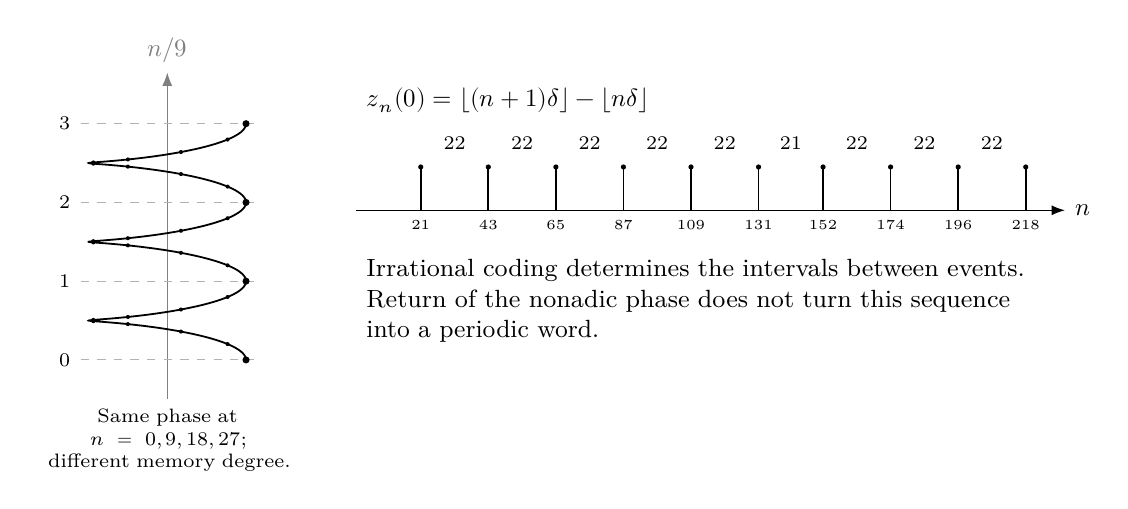
\begin{tikzpicture}[x=1cm,y=1cm,>=Latex,font=\small]
\begin{scope}[xshift=1.8cm,yshift=.3cm]
\draw[->,gray] (0,-.5)--(0,3.65) node[above] {\(n/9\)};
\foreach \k in {0,1,2,3}{
 \draw[gray!60,dashed] (-1.1,\k)--(1.1,\k);
 \node[left,font=\scriptsize] at (-1.1,\k){\(\k\)};
}
\draw[black,line width=.65pt,domain=0:27,samples=260,smooth,variable=\n]
 plot ({cos(40*\n)},{\n/9+.14*sin(40*\n)});
\foreach \n in {0,...,27}{
 \fill ({cos(40*\n)},{\n/9+.14*sin(40*\n)}) circle (.026);
}
\foreach \k in {0,1,2,3}{\fill (1,\k) circle (.045);}
\node[align=center,text width=3.3cm,font=\scriptsize] at (0,-1.02)
 {Same phase at \(n=0,9,18,27\);\\different memory degree.};
\end{scope}
\begin{scope}[xshift=4.2cm,yshift=.5cm]
\node[anchor=west] at (0,3.1){\(z_n(0)=\lfloor(n+1)\delta\rfloor-\lfloor n\delta\rfloor\)};
\draw[->] (0,1.7)--(9,1.7) node[right]{\(n\)};
\foreach \n in {21,43,65,87,109,131,152,174,196,218}{
 \draw[line width=.6pt] ({\n*.039},1.7)--({\n*.039},2.25);
 \fill ({\n*.039},2.25) circle (.033);
 \node[below,font=\tiny] at ({\n*.039},1.7){\n};
}
\foreach \a/\b/\g in {21/43/22,43/65/22,65/87/22,87/109/22,109/131/22,131/152/21,152/174/22,174/196/22,196/218/22}{
 \node[font=\scriptsize] at ({(\a+\b)*.0195},2.55){\g};
}
\node[anchor=west,align=left,text width=8.3cm] at (0,.55)
 {Irrational coding determines the intervals between events. Return of the nonadic phase does not turn this sequence into a periodic word.};
\end{scope}
\end{tikzpicture}
\caption{Complementary representations of transport. Left: projection of the helix \((\cos(2\pi n/9),\sin(2\pi n/9),n/9)\): advancing nine steps recovers the phase and increases the height. Right: the first ten events of the lower word for \(\delta=\log_{10}(10/9)\), with exact separations \(21\) or \(22\). The helical representation introduces no additional physical metric.}
\label{fig:holonomia-esturmiana}
\end{figure}


For this count we fix the intercept \(\theta=0\) and cumulative endpoints
\[
(N_0,\ldots,N_4)=(0,729,972,999,1000),
\]
corresponding to the cubic order \((729,243,27,1)\). The lower counts are \(\lfloor N_j\delta\rfloor-\lfloor N_{j-1}\delta\rfloor\), giving \((33,11,1,0)\). The upper counts are \(\lceil N_j\delta\rceil-\lceil N_{j-1}\delta\rceil\), with the same initial boundary zero, giving \((34,11,1,0)\). These values depend on the intercept and the order of the strata; they are not asserted for an arbitrary initial phase. Their totals are forty-five and forty-six. The increment corresponds to a single boundary unit, located in the first stratum of this ordered partition. The numbers thirty-four and eleven thus appear in the same count before any units chart; identifying them with physical exponents additionally requires the corresponding dimensional derivation.

The term \emph{aperiodic crystal} is used here for this symbolic order, with complexity, spectrum, and return specified. Zero topological entropy does not by itself imply zero physical dissipation: a thermodynamic realization requires a defined energetic dynamics and erasure operation. Likewise, this Sturmian reading does not replace all TPK operators or by itself prove periodicity or aperiodicity of the complete \(\alpha\) output. Its function is to make explicit a structure of order that the mere return of the calendar does not describe.

% Cumulative addition. Insert after the existing Sturmian suspension.
% Preserve the full text and figure fig:holonomia-esturmiana.
\subsection{Nonadic connection, holonomy, and monodromy representation}
\label{mono-ampl:conexion}

The regional structure requires distinguishing the transport producing a
history, observation of its phase, and representation of its returns.
APP supplies the two arithmetic evaluations with remainder and quotient; TRIT
determines regime and orientation; the Topological Phase Kernel composes
selection, transport, and update. The initial conditions of
cardinality \(104\,976\), their catalog of \(468\) emissions, and the \(243\)
visible words in the ambient space of \(729\) elements belong to different
stages of that construction. The chain
\[
 w_6\longrightarrow w_{12}\longrightarrow w_{18}
 \longrightarrow w_{24}\longrightarrow w_{30}
 \longrightarrow R_{36}\longrightarrow G_9
\]
leads to a joint connection over the three regions. Its nine phases
are positions of a single transport, and the regional coordinates
\(\pi,\varphi,e\), together with the dodecaphasic determination of \(\alpha\),
arise from its compatible readings\cite{hmtintegral,hmtholonomia}.

At prolongation index \(k\), a state chart preserves
\[
 \widehat x_k=(B_k,C_k,p_k,c_k,\Sigma_k,W_k,g_k,m_k).
\]
Here \(B_k\) collects the three regional blocks, \(C_k\) is the cylinder,
\(p_k\) the prefix, \(c_k\) the carry record, \(\Sigma_k\) the boundary
signature, and \(W_k\) the incidence information. The phase is
\(g_k=1+[(k-1)]_9\); \(m_k\) counts complete turns. The reduction
\(\beta_k=[m_k]_{12}\) preserves the dodecaphasic position, whereas the
integer \(m_k\) distinguishes its successive turns.

\begin{definition}[Transport through one nonadic turn]
\label{mono-ampl:def-vuelta}
Let \(\mathcal R_k\subseteq\widehat X_k\times\widehat X_{k+1}\)
be the admissible extension relations of the TPK. The realization of
holonomy at level \(k\) is the relational composition
\[
 \Gamma_{9,k}=\mathcal R_{k+8}\circ\cdots\circ\mathcal R_k.
\]
For \(s\geq1\), its prolongation through \(s\) turns is
\[
 \Gamma_{9s,k}=
 \Gamma_{9,k+9(s-1)}\circ\cdots\circ\Gamma_{9,k}.
\]
\end{definition}

The relational formulation preserves admissible continuations. On
an individualized history, each arrow leads to the state actually
prolonged; the isolated visible block may still admit more than one
continuation. This difference is precisely the function of memory and
boundary conditions in determining the trajectory.

\begin{proposition}[Iteration of return and accumulated memory]
\label{mono-ampl:vueltas}
In every admissible composition of \(s\) turns,
\[
 g_{k+9s}=g_k,\qquad m_{k+9s}=m_k+s,\qquad
 \beta_{k+9s}=\beta_k+s\pmod{12}.
\]
\end{proposition}
\begin{proof}
The one-turn rule preserves the phase and increments the counter by one.
Applying it to the already transported state repeats exactly these
two operations. Induction gives the first two equalities; reducing the
second modulo \(12\) gives the third.
\end{proof}

The counter thus provides an integer witness of the difference between
turns. After \(12\) turns the pair of finite phases is restored, but
the counter increases by \(12\). The nonsplit extension
\eqref{eq:extension108} expresses the composition of the calendar through its
cocycle; the trajectory also preserves the integer lift of that datum.
Preservation here means transport of prior contributions,
not immobility of all coordinates.

\Needspace{9\baselineskip}
\subsubsection{Bilateral representation of the return index}

The geometric realization of the cyclic graph admits an especially simple
operator representation. Here we number the phases from \(0\) to
\(8\), shifting the origin relative to \(g_k\), and
write \(k=9m+r\), with \(0\leq r<9\), on the integer line
covering the phase cycle. On
\(\mathcal H_{\rm ind}=\ell^2(\mathbb Z)\), the basis
\(|k\rangle=|r,m\rangle\) allows the unit shift to be expressed as
\[
 T|r,m\rangle=
 \begin{cases}
 |r+1,m\rangle,&r<8,\\
 |0,m+1\rangle,&r=8.
 \end{cases}
\]
The inverse decreases \(r\) by one when \(r>0\), and sends
\(|0,m\rangle\) to \(|8,m-1\rangle\). Passing through the phase origin
therefore incorporates the exact unit of quotient.

\begin{proposition}[Representation of cycle monodromy]
\label{mono-ampl:representacion}
Let \(S=T^9\). Then
\[
 S|r,m\rangle=|r,m+1\rangle,\qquad
 \mathbb Z\longrightarrow\mathcal U(\mathcal H_{\rm ind}),
 \quad s\longmapsto S^s
\]
is a faithful unitary representation of the group of turns of the cycle.
\end{proposition}
\begin{proof}
Nine shifts preserve the remainder of division by \(9\) and
increment the quotient. The powers satisfy
\(S^{s+t}=S^sS^t\), and \(S^s|r,m\rangle=|r,m+s\rangle\) distinguishes
every integer \(s\). A permutation of an orthonormal basis is unitary.
\end{proof}

This representation corresponds to the covering of the cycle, whose group
of turns is \(\mathbb Z\), and represents the phase with its counter. The
TPK state also contains the trajectory coordinates already described.
The bilateral extension admits negative indices as coordinates of the
covering; a trajectory beginning at an initial condition uses
its admissible half-axis. An operator inverse of the index is thus available
without turning every extension relation into a bijection of the
full state.

With \(D_M|k\rangle=\lfloor k/9\rfloor|k\rangle\), the identity
\([D_M,S]=S\) expresses the memory increment on the dense domain of
finitely supported vectors. If \(\mathcal I|k\rangle=|-k\rangle\) and
\(P_0\) projects onto indices divisible by \(9\), one also obtains
\begin{equation}
 \mathcal I T\mathcal I=T^{-1},\qquad
 \mathcal I D_M\mathcal I=-D_M-(I-P_0).
 \label{mono-ampl:inversion-contador}
\end{equation}
Indeed, for \(k=9m+r\),
\(\lfloor-k/9\rfloor=-m\) if \(r=0\), and equals \(-m-1\) if \(r>0\).
Inversion thus preserves the boundary term of Euclidean division.

\subsection{Block clock and capacity clock}
\label{mono-ampl:relojes}

The index of a refinement map and the number of available decimal
positions obey related but different laws. To express
them, reserve \(n\) for the ternary-block index and define
\[
 \rho=\log_{1000}729=\log_{10}9,\qquad
 \delta=1-\rho,\qquad
 \mathcal C_n=\lfloor(n+1)\rho\rfloor,\quad n\geq0.
\]
Here \(\mathcal C_n\) denotes capacity, not the dodecaphasic
record \(K\). At the canonical phase origin, the preceding mechanical
word provides
\[
 Z_n=\sum_{j=0}^{n}z_j(0)=\lfloor(n+1)\delta\rfloor.
\]

\begin{proposition}[Exact balance between capacity and vacancies]
\label{mono-ampl:balance-capacidad}
For \(n\geq0\), and in the second identity for \(n\geq1\),
\[
 \mathcal C_n=n-Z_n,\qquad
 \mathcal C_n-\mathcal C_{n-1}=1-z_n(0).
\]
\end{proposition}
\begin{proof}
Irrationality of \(\delta\) implies
\(\lceil(n+1)\delta\rceil=\lfloor(n+1)\delta\rfloor+1\).
Then
\[
 \lfloor(n+1)(1-\delta)\rfloor
 =n+1-\lceil(n+1)\delta\rceil=n-Z_n.
\]
Subtracting two consecutive identities concludes the proof.
\end{proof}

An event \(z_n=1\) adds a block to the history while preserving capacity
\(\mathcal C_n\); an event \(z_n=0\) increments both counters. Over
any interval, capacity increments and vacancies sum
exactly to its length. Reducing modulo \(q\), for \(q=9\) or
\(q=108\), gives
\[
 [\mathcal C_n]_q=[n]_q-[Z_n]_q.
\]
The uniform block phase and capacity phase are related through
the integrated memory of vacancies. In particular, a capacity
hold and a complete turn of the connection have distinct
mechanisms, although both may preserve a phase observation.

Monotone inversion of the clock gives a first-arrival time:
\[
 T_{\rm cap}(a)=\min\{n:\mathcal C_n=a\}
 =\left\lceil\frac a\rho\right\rceil-1,
 \qquad a\geq1.
\]
With \(\sigma=\rho^{-1}-1\), the time needed to gain \(b\) units
of capacity is
\[
 T_{\rm cap}(a+b)-T_{\rm cap}(a)
 =b+\lceil(a+b)\sigma\rceil-\lceil a\sigma\rceil.
\]
The difference of ceilings takes one of the two integers adjacent to
\(b\sigma\). This yields \(9\) or \(10\) blocks to gain
\(9\) capacity units, and \(113\) or \(114\) to gain \(108\).
These are inverse-clock times measured from a first arrival; the
turn counter is always interpreted in the index to which it belongs.

\subsection{Symbolic suspension and aperiodic time crystal}
\label{mono-ampl:cristal}

Rotation coding combines phase periodicity, local recurrence,
and global aperiodicity. Let \(\mathcal X_\delta\subseteq\{0,1\}^{\mathbb Z}\)
be the closure, in the product topology, of shifts of the bilateral
word \(z_n(\theta)\). Denote by \(\sigma_{\rm sh}\) the
shift of its sequences. Retaining a nonadic phase, the step is
\[
 F(r,z)=([r+1]_9,\sigma_{\rm sh}z),\qquad
 (r,z)\in C_9\times\mathcal X_\delta.
\]

\begin{definition}[Symbolic aperiodic time crystal]
\label{mono-ampl:def-cristal}
The unit-roof suspension of the preceding system is the space
\[
 \mathcal S_\delta=
 \bigl((C_9\times\mathcal X_\delta)\times\mathbb R\bigr)/\sim,
 \qquad (y,t+1)\sim(Fy,t),
\]
with flow \(\Phi_s[y,t]=[y,t+s]\). This model of temporal order,
together with its vacancy coding and turn-counter representation,
is called a \emph{symbolic aperiodic time crystal}.
\end{definition}

The adjective temporal designates the action of the flow and its return section;
aperiodicity characterizes its itineraries. The frequency of ones in each
sequence is \(\delta\): the uniform discrepancy bound of less than one,
obtained by telescoping over any window, persists under closure.
A periodic sequence would have rational frequency. Therefore,
\(\mathcal X_\delta\) contains no periodic orbits. Nor does the suspension
have closed orbits: a return of the flow would require an integer
time and periodicity of the itinerary.

Finite words do recur. Length-\(m\) itineraries
come from a partition of the circle by \(m+1\) points; every
interval is visited recurrently by irrational rotation. Even
when times are restricted to a fixed phase, the step \(9\delta\) remains
irrational. This is why every word appears in all
\(9\) phases and explains the already established complexities
\[
 p(m)=m+1,\qquad p_9(m)=9(m+1),\qquad p_3(m)=3(m+1).
\]
Recurrence of local configurations coexists with the absence of a
global period. Its topological entropy is zero because these complexities
grow linearly.

The realization through observables \(V_9,W_\delta\) and the shift
\(T\) expresses the same order through the covariances
\eqref{eq:weyl-relojes}. The frequencies of the uniform clock belong to
\(\frac19\mathbb Z+\delta\mathbb Z\), modulo \(1\). The capacity
clock additionally preserves the relation
\([\mathcal C_n]_9=[n]_9-[Z_n]_9\); it is not replaced by the uniform phase
when returns are interpreted. The term \emph{time crystal} is thus
defined through a mathematical dynamical system. Its physical realization
requires specifying an energetic dynamics, its temporal observables,
and its stability, data distinct from the present symbolic construction.

\subsection{Specular symmetry of the regions and dual realization}
\label{mono-ampl:regiones}

Specular exchange acts on the regional block
\(B=(u^\pi,u^e,u^\varphi)\in(\mathbb F_3^6)^3\) by
\[
 \mathfrak cB=(u^e,u^\pi,u^\varphi).
\]
Its fixed axis and aggregate are, respectively, \(u^\varphi\) and
\(s=u^\pi+u^e\). This fixedness concerns the involution in a fiber;
both coordinates may evolve during nonadic transport.
With \(q=u^\pi+u^e+u^\varphi\),
\(a=u^\pi+u^e-u^\varphi\), and \(d=u^\pi-u^e\), one recovers
\[
 u^\varphi=2(q-a),\qquad s=q-u^\varphi,\qquad
 u^\pi=2(s+d),\qquad u^e=2(s-d).
\]
The equalities hold componentwise in \(\mathbb F_3\), where
\(2^{-1}=2\). The mirror preserves \(q,a,s\) and reverses \(d\); this
antisymmetric coordinate individualizes the allocation that the aggregate preserves
without distinguishing. Time-index inversion \(\mathcal I\) and the
channel involution \(\mathfrak c\) therefore act on
different data.

Phase return has an explicit witness:
\[
 \begin{aligned}
 B_1&=(012222\mid121221\mid112202),\\
 B_{10}&=(101222\mid112221\mid112002).
 \end{aligned}
\]
Both positions have phase \(1\); the block, axis, and memory have
changed. Likewise, census synchronization in phases \(8\) and
\(9\) annihilates their relative differences, while the diagonal component
passes from \((59,59,59)\) to \((43,43,43)\). Equality of a relative
observable does not exhaust the state determining it.

The dual realization preserves this architecture. In section
\ref{exc:doble-lectura}, the same prefix determines nested
cylinders on one side and a sequence of encoded words with their frames on the other.
The first map passes to the limit by contraction of diameters; the second
satisfies \(r_{n,m}Q_n=Q_mp_{n,m}\) and defines \(Q_\infty\).
Figure \ref{mono-ampl:fig-regional} anticipates these two maps.
The subsequent incidence construction produces codes, lattices, and the
Moonshine realization in their own domains; the automorphism group
acts on that realization, not on the digits through an implicit
identification.

% Figura acumulativa; destino figures/monodromia_regional_ampliacion.tex.
\begin{figure}[!htbp]
\centering
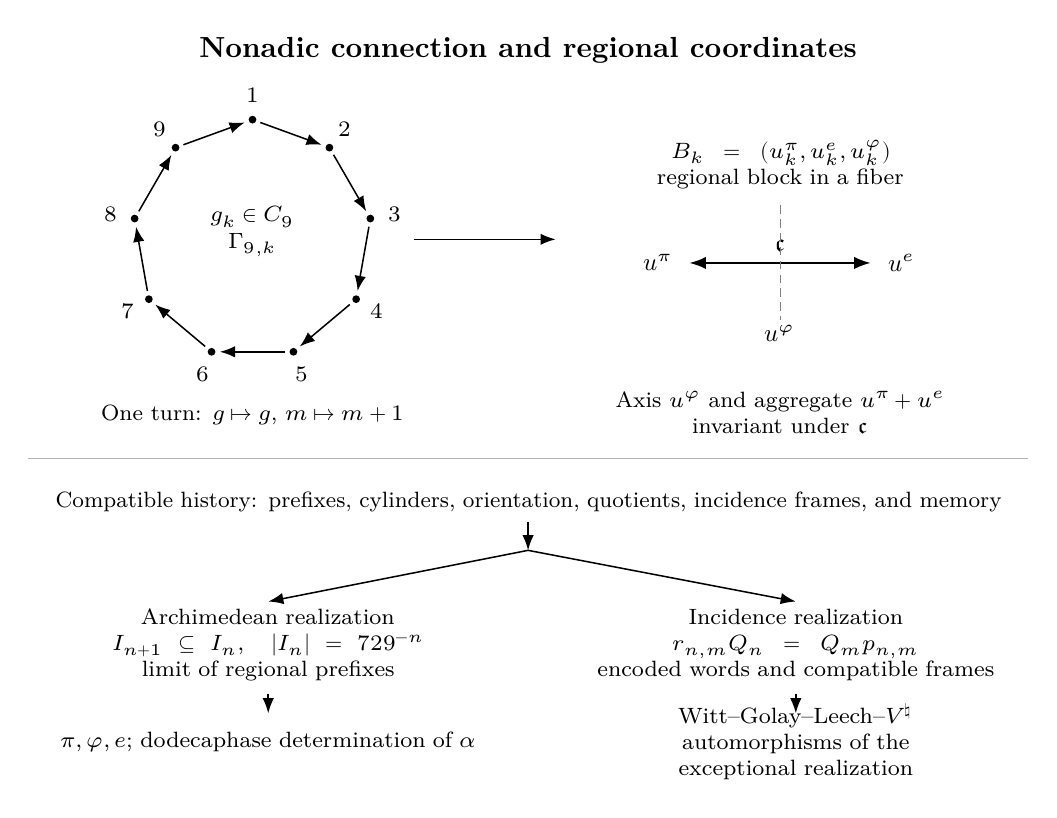
\begin{tikzpicture}[x=1cm,y=1cm,>=Latex,font=\small,
  flow/.style={->,line width=.55pt},
  ann/.style={align=center,font=\footnotesize}]
\node[font=\bfseries] at (6.9,9.2)
  {Nonadic connection and regional coordinates};
\begin{scope}[shift={(3.4,6.8)}]
 \foreach \k in {1,...,9}{
  \pgfmathsetmacro{\ang}{90-40*(\k-1)}
  \coordinate (p\k) at (\ang:1.52);
  \fill (p\k) circle (1.4pt);
  \node[fill=white,inner sep=1.1pt,font=\footnotesize]
    at (\ang:1.83) {\(\k\)};
 }
 \foreach \k in {1,...,8}{
  \pgfmathtruncatemacro{\next}{\k+1}
  \draw[flow,shorten >=3pt,shorten <=3pt] (p\k)--(p\next);
 }
 \draw[flow,shorten >=3pt,shorten <=3pt] (p9)--(p1);
 \node[ann] at (0,.1) {\(g_k\in C_9\)\\\(\Gamma_{9,k}\)};
 \node[ann] at (0,-2.23) {One turn: \(g\mapsto g\), \(m\mapsto m+1\)};
\end{scope}
\node[ann,text width=5.25cm] at (10.1,7.75)
 {\(B_k=(u_k^\pi,u_k^e,u_k^\varphi)\)\\
 regional block in a fiber};
\node at (8.55,6.5) {\(u^\pi\)};
\node at (11.65,6.5) {\(u^e\)};
\draw[<->,line width=.65pt] (8.95,6.5)--node[above]{\(\mathfrak c\)}(11.25,6.5);
\draw[densely dashed,gray] (10.1,5.72)--(10.1,7.23);
\node[fill=white,inner sep=2pt] at (10.1,5.6){\(u^\varphi\)};
\node[ann] at (10.1,4.6)
 {Axis \(u^\varphi\) and aggregate \(u^\pi+u^e\)\\
 invariant under \(\mathfrak c\)};
\draw[flow] (5.45,6.8)--(7.25,6.8);
\draw[gray!60,line width=.3pt] (.55,4.02)--(13.25,4.02);
\node[ann,text width=12cm] (hist) at (6.9,3.47)
 {Compatible history: prefixes, cylinders, orientation, quotients,
 incidence frames, and memory};
\coordinate (fork) at (6.9,2.85);
\draw[flow] (hist.south)--(fork);
\draw[flow] (fork)--(3.6,2.2);
\draw[flow] (fork)--(10.3,2.2);
\node[ann,text width=5.6cm] at (3.6,1.65)
 {Archimedean realization\\
 \(I_{n+1}\subseteq I_n,\quad |I_n|=729^{-n}\)\\
 limit of regional prefixes};
\node[ann,text width=5.6cm] at (10.3,1.65)
 {Incidence realization\\
 \(r_{n,m}Q_n=Q_mp_{n,m}\)\\
 encoded words and compatible frames};
\node[ann,text width=5.6cm] at (3.6,.42)
 {\(\pi,\varphi,e\); dodecaphase determination of \(\alpha\)};
\node[ann,text width=5.6cm] at (10.3,.42)
 {Witt--Golay--Leech--\(V^\natural\)\\
 automorphisms of the exceptional realization};
\draw[flow] (3.6,1.03)--(3.6,.78);
\draw[flow] (10.3,1.03)--(10.3,.78);
\end{tikzpicture}
\caption{\fontsize{9}{11}\selectfont Nine phases of a connection and two realizations of a compatible
history. The cycle represents phase; each turn increments the counter.
The regional diagram represents the involution \(\mathfrak c\), which
interchanges closure and propagation and fixes the self-scaling axis in a fiber.
This invariance does not require the axis to remain constant during transport.
The two lower maps use the same prefix: one determines its numerical limit,
while the other preserves words and incidence frames. The maps of the second
realization are specified in Section \ref{exc:doble-lectura}; the exceptional
construction is developed afterwards.}
\label{mono-ampl:fig-regional}
\end{figure}


\subsection{Temporal transport and tritic exponential composition}
\label{mono-ampl:euler}

The Euler relations in section \ref{euler-trit-articulacion}
describe local realizations of the three regimes. For a fixed
signature \(\tau\), the generator satisfies \(J_\tau^2=-\tau I\); algebraic
conjugation sends \(J_\tau\) to \(-J_\tau\). Consequently,
\[
 \exp(sJ_\tau)\exp(tJ_\tau)=\exp((s+t)J_\tau),\qquad
 \overline{\exp(tJ_\tau)}=\exp(-tJ_\tau),
\]
and the product of an evolution with its conjugate is the unit. In the elliptic
type it is realized through \(\cos^2t+\sin^2t=1\); in the hyperbolic type,
through \(\cosh^2t-\sinh^2t=1\); in the parabolic type,
\((I+tN)(I-tN)=I\), since \(N^2=0\). The same conservation law
admits three quadratic expressions.

The elliptic realization closes a turn; the nilpotent one preserves a
linear displacement; the hyperbolic one separates expansion and contraction with
unit determinant. At the regional parameters already generated,
\[
 \exp(\pi J_{\mathrm e})=-I,\qquad
 \exp(J_{\mathrm p})=I+J_{\mathrm p},\qquad
 \exp(2\log\varphi\,J_{\mathrm h})=F_{\rm av}^{\,2}.
\]
The evaluation \(\exp(I)=eI\) recognizes the unit of the common
exponential law. The number \(e\) is not assigned exclusively to the parabolic regime.

Transporting a local realization through an isomorphism \(U\) preserves
these relations: if \(J'=UJU^{-1}\), the exponential series gives
\(U\exp(tJ)=\exp(tJ')U\). The identity transports the regime and its
norm. A transition between different quadratic types, by contrast, belongs
to TPK sheet and regime selection; it is not a conjugation
changing the value of \(J^2\). The temporal product therefore preserves the
order of transitions and the information at their endpoints.

This articulation distinguishes the closure of a local representation from the
holonomy of a history. One may have \(\exp(2\pi J_{\mathrm e})=I\)
at the same time as \(S|r,m\rangle=|r,m+1\rangle\). The first equality
restores the regime's orientation; the second records another turn. The
discrete structure preserves both: the local return and the accumulated
provenance of the state realizing it.


% Recovery of the native product and its selector, not incorporation of RH.
\subsection{Multiplicative irreducibility and return periods}
\label{primos-retornos}

The distinction between structure, evaluation, and phase also appears in
the multiplicative sector. APP's local product contains both residue and
quotient; iterating it constructs normal forms and factorizations before
their decimal periods are examined. This development places the expression
\emph{prime mode} in a precise domain and relates irreducibility to the
operations already defined, rather than to an isolated coincidence
of periods \cite{hmtintegral,hmtholonomia}.

Let
\[
 \mathcal W_9=\{\varnothing\}\sqcup
 \bigsqcup_{\ell\geq1}\{1,\ldots,9\}^{\ell}.
\]
Sequences are ordered from the least significant digit. The evaluation
\(\operatorname{ev}_9(u)=\sum_j u_j9^j\), with
\(\operatorname{ev}_9(\varnothing)=0\), is bijective onto the nonnegative
integers: for a positive integer, division of \(n-1\) by \(9\)
uniquely determines the first digit and continuation. This is bijective
nonadic numeration; it retains the boundary representative \(9\).

Addition \(\boxplus_\#\) is obtained by applying APP's additive sheet
to the digits at each position and propagating their quotients. If there
is only one digit, it is the provisional residue; a nonzero incoming
quotient is normalized through a second additive operation. The sum of
quotients is transported to the next position. To multiply a sequence by
a digit \(d\), the multiplicative cell produces
\(u_jd=9q_j+r_j\), and the incoming quotient \(c_j\) is incorporated by
\[
 (w_j,c_{j+1})=
 \begin{cases}
 (r_j,q_j),&c_j=0,\\
 \bigl(R^+(r_j,c_j),q_j+q^+(r_j,c_j)\bigr),&c_j>0.
 \end{cases}
\]
Start with \(c_0=0\) and incorporate the final quotient when nonzero.
During addition, \(c_j\leq2\); during multiplication by a digit,
\(c_j\leq9\). Local operations thus receive arguments within
their domain. Denote this second procedure by \(d\odot_\#u\),
with \(d\odot_\#\varnothing=\varnothing\).

For \(v=(v_0,\ldots,v_{m-1})\), the complete product is constructed
through the recurrence
\[
 a_m=\varnothing,\qquad
 a_j=(9\odot_\#a_{j+1})\boxplus_\#(v_j\odot_\#u),
 \qquad u\boxtimes_\#v=a_0.
\]
The rule composes both local sheets. Its evaluation satisfies
\begin{equation}
 \operatorname{ev}_9(u\boxtimes_\#v)
   =\operatorname{ev}_9(u)\operatorname{ev}_9(v).
 \label{eq:primos-entrelazamiento}
\end{equation}
Indeed, each transition preserves the partial sum plus the pending
quotient weighted by the power of \(9\). The recurrence then gives
\(\operatorname{ev}_9(a_j)=9\operatorname{ev}_9(a_{j+1})+
v_j\operatorname{ev}_9(u)\), whose iteration proves
\eqref{eq:primos-entrelazamiento}. Uniqueness of normal form transports
associativity and commutativity to the constructed product; its identity is \((1)\).

\begin{definition}[Reduced multiplicative coproduct]
On the finitely supported vector space generated by nonempty normal
forms, define
\[
 \widetilde\Delta_\# e_w
 =\sum_{\substack{u\boxtimes_\#v=w\\u,v\ne(1)}}e_u\otimes e_v.
\]
A non-unit normal form is irreducible when its image under
\(\widetilde\Delta_\#\) is zero.
\end{definition}

Factorization fibers are finite by
\eqref{eq:primos-entrelazamiento}. In the completion
\(\mathcal H_\#=\ell^2(\mathcal W_9\setminus\{\varnothing\})\),
images of distinct forms have disjoint supports. If \(d_\#(w)\)
counts ordered non-unit factorizations, the domain of the closure is
\[
 \operatorname{Dom}(\overline{\widetilde\Delta_\#})
 =\left\{x\in\mathcal H_\#:
       \sum_w d_\#(w)|x_w|^2<\infty\right\}.
\]
Indeed, the squared norm of the image is this weighted sum. Hence
the operator
\[
 A_\#=(\overline{\widetilde\Delta_\#})^*
                  \overline{\widetilde\Delta_\#}
\]
is diagonal, positive, and self-adjoint: its eigenvalue at \(e_w\)
is the number of ordered non-unit factorizations of \(w\). The projection
\[
 P_{\rm irr}=(I-|e_{(1)}\rangle\langle e_{(1)}|)
                    \mathbf1_{\{0\}}(A_\#)
\]
selects exactly the irreducible forms. Through multiplicative evaluation,
these correspond to ordinary primes. Selection depends on factorization
structure and keeps the unit state separate.

For a value \(n\geq2\) coprime to \(10\), decimal division induces
the residue permutation \(r\mapsto10r\pmod n\). Return of residue
\(1\) has period
\[
 \tau_n=\operatorname{ord}_n(10).
\]
If \(n=\prod_p p^{a_p}\), the Chinese remainder theorem gives
\[
 \tau_n=\operatorname{lcm}_{p^{a_p}\parallel n}
                    \operatorname{ord}_{p^{a_p}}(10).
\]
Composite return synchronizes the returns of prime powers.
For a prime \(p\notin\{2,3,5\}\),
\[
 \tau_p\mid p-1,\qquad
 M_p=\frac{10^{\tau_p}-1}{p}\in\mathbb N,
 \qquad M_p\equiv0\pmod9.
\]
The last congruence expresses nonadic closure of decimal repetition:
\(10^{\tau_p}-1\) is a multiple of \(9\), and \(p\) is invertible
modulo \(9\). The same congruence holds for every \(n\) coprime
to \(90\). In particular, \(7,13,77,91,143\) have decimal period
\(6\), although only the first two are irreducible. The coproduct and
the period therefore record different properties of the same constructed value.

This differentiation specifies the relation with aperiodic refinement.
The vacancy sequence determines increments of the capacity index;
factorization determines multiplicative modes; decimal division
determines their return times. The nonadic representative preserves
phase closure, while quotient and factorization retain information
that this closure does not distinguish. The connection to the treatise's
spectral constructions resides in these operators and their intertwinings.
Proof of their subsequent analytic results retains its own development;
it is not replaced by periodicity of a residue observation.

\subsubsection{Vacancy discrepancy and Dirichlet readings}

The connection also admits an exact analytic expression. Retain the
same coding \(z_n=z_n(0)\), for \(n\geq1\), and consider two
subsequent observables: the series over all indices and the product
over indices selected by irreducibility. For \(\operatorname{Re}s>1\),
\[
 Z_{\rm vac}^{+}(s)=\sum_{n\geq1}\frac{z_n}{n^s},\qquad
 Z_{\rm vac}^{\times}(s)=\prod_p(1-p^{-s})^{-z_p}.
\]
Both converge absolutely in this half-plane. Their common factor is
density \(\delta\), but their discrepancies differ.

\Needspace{21\baselineskip}
\begin{proposition}[Separation of vacancy density]
We have
\[
 Z_{\rm vac}^{+}(s)=\delta\zeta(s)+H_{\rm vac}(s),
 \qquad H_{\rm vac}\in\mathcal O(\operatorname{Re}s>0).
\]
In \(\operatorname{Re}s>1\), with logarithms defined by absolutely
convergent Euler series,
\[
 Z_{\rm vac}^{\times}(s)=\zeta(s)^\delta G_{\rm vac}(s),\qquad
 \log G_{\rm vac}(s)=
 \sum_p(z_p-\delta)\log(1-p^{-s})^{-1}.
\]
\end{proposition}
\begin{proof}
The centered partial sums satisfy
\[
 A_N:=\sum_{n=1}^N(z_n-\delta)
 =\lfloor(N+1)\delta\rfloor-N\delta,\qquad |A_N|<1.
\]
Abel summation represents the centered term by
\(s\int_1^\infty A_{\lfloor x\rfloor}x^{-s-1}\,dx\).
The integral converges locally uniformly in \(\operatorname{Re}s>0\),
proving holomorphy. The second identity follows by separating
\(z_p=\delta+(z_p-\delta)\) in the logarithm of the product,
within its domain of absolute convergence.
\end{proof}

The decomposition reveals what the reading on primes adds: it examines
the same vacancy sequence on a subset determined by factorization.
Controlling discrepancy over all integers gives the first holomorphic
continuation; the second observable preserves its own discrepancy on
primes. These are two applications of the same discrete structure,
with explicit analytic domains. This articulation explains their
relevance to the arithmetic kernel without transferring the proof
of the treatise's terminal results to this article.


\clearpage% BEGIN NUCLEO_ADITIVO_20260921_SELECCION
\clearpage
% Demonstrative expansion DF003--DF007. The integral source is unchanged.
% Common owner of the Lean files cited in these comments:
% output/PAQUETE_ARTICULO_I_INTEGRACION_ESTADO_CAMPOS_20260919/.
% Causal placement of the first section: after the coinductive regional
% readers and before their registers are used as inputs to K selection.
% Causal placement of the second section: after the marked
% Paley--Witt--Golay--Leech construction and before reconstruction of the VOA.
% Both expository cuts preserve the same APP--TRIT--TPK origin.

\section[Regional generation and refinement]{Integral compatibility of regional generation, cylindrical refinement, and incidence}
\label{act21:sec:df-lectores-cilindros}

Regional prolongation produces ordered sequences of blocks together with
their reading depths. The Archimedean projection and ternary incidence
are calculated on these same sequences. The connection between the two
realizations can be formulated entirely through integer operations:
selection by rational intervals, Euclidean division, lifting of six
trits, carry reading, and the Witt transformation. This formulation makes
it possible to trace each coefficient from its generating block to its
subsequent use.

The construction uses the three regional readers already obtained from the
APP--TRIT--TPK state. We denote them by the indices
\(c\in\{\mathrm P,\mathrm E,\mathrm F\}\), corresponding, respectively,
to the closure, propagation, and autoscaling regions. Their real realization
will be written as \(v_c\). The subsequent identifications
\(v_{\mathrm P}=\pi_{\mathrm{HMT}}\),
\(v_{\mathrm E}=e_{\mathrm{HMT}}\), and
\(v_{\mathrm F}=\varphi_{\mathrm{HMT}}\) preserve this causal order.
The operation that emits a block inspects the rational intervals of the
regional reader; the real value enters the proof of correctness of that
operation.

\subsection{Positional emission through rational separation of cells}
\label{act21:subsec:df-emision-racional}

% Source: lean/biblioteca/RegionalPublicationComposition.lean,
% produced_brackets, eventual_publication, joint_eventual_publication,
% search_terminates, stopped_cell_correct, publications_compatible.

For each region, two rational sequences
\(\ell_c(j),u_c(j)\), constructed by its reader, are available and satisfy
\[
 \ell_c(j)\leq v_c\leq u_c(j).
\]
The cell-separation property proved for these readers states that, for
each integer \(s>0\), there exists \(J\) such that, for every \(j\geq J\),
\begin{equation}
 \lfloor s\ell_c(j)\rfloor
 =\lceil su_c(j)\rceil-1
 =\lfloor sv_c\rfloor.
 \label{act21:eq:df-separacion-celdas}
\end{equation}
Avoidance of rational boundaries by the regional values is the hypothesis
of the preceding theorems that guarantees this separation. Here we use
their operational conclusion together with the readers and intervals
that produce it.

\begin{definition}[Separation index and emitted prefix]
For \(s>0\), let
\[
 j_c(s)=\min\{j\in\mathbb N:
 \lfloor s\ell_c(j)\rfloor=\lceil su_c(j)\rceil-1\}.
\]
For an integer base \(b\geq2\) and a depth \(n\geq0\), define
\begin{equation}
 P_c(b,n)=\lfloor b^n\ell_c(j_c(b^n))\rfloor.
 \label{act21:eq:df-publicacion-prefijo}
\end{equation}
The prefix contains the integer part and the first \(n\) positions in base
\(b\); consequently, \(P_c(b,0)\) is the regional integer part.
\end{definition}

\begin{theorem}[Termination and correctness of emission]
\label{act21:thm:df-emision-correcta}
The index \(j_c(s)\) exists for every \(s>0\). The emitted prefixes satisfy
\begin{equation}
 P_c(b,n)=\lfloor b^n v_c\rfloor,
 \qquad
 P_c(b,n)\leq b^n v_c<P_c(b,n)+1.
 \label{act21:eq:df-prefijo-correcto}
\end{equation}
For each scale \(s\), a single sufficiency index \(J(s)\) can also be
chosen that is valid simultaneously for all three regions.
\end{theorem}

\begin{proof}
The eventual equality in \eqref{act21:eq:df-separacion-celdas} makes the set
defining \(j_c(s)\) nonempty. Its minimum exists by the well-ordering of
\(\mathbb N\). At any index where the equality holds, the rational lower
bound gives
\(\lfloor s\ell_c(j)\rfloor\leq\lfloor sv_c\rfloor\).
The upper bound, together with avoidance of a cell boundary, gives
\(\lfloor sv_c\rfloor\leq\lceil su_c(j)\rceil-1\).
When the two integer endpoints coincide, the intervening integer coincides
with them. This proves \eqref{act21:eq:df-prefijo-correcto}. For the joint
statement, it suffices to take the maximum of the three sufficiency indices
obtained at the same scale. The joint index controls all three emissions
simultaneously, while each region retains its own intervals.
\end{proof}

\begin{proposition}[Exact compatibility of prefixes]
\label{act21:prop:df-prefijos-compatibles}
For \(n,m\geq0\),
\begin{equation}
 \left\lfloor\frac{P_c(b,n+m)}{b^m}\right\rfloor=P_c(b,n).
 \label{act21:eq:df-truncamiento}
\end{equation}
In particular, the next block
\(d_c(b,n)=P_c(b,n+1)\bmod b\) satisfies
\begin{equation}
 P_c(b,n+1)=bP_c(b,n)+d_c(b,n),\qquad 0\leq d_c(b,n)<b.
 \label{act21:eq:df-paso-posicional}
\end{equation}
\end{proposition}

\begin{proof}
Write \(b^n v_c=N+\theta\), with
\(N=P_c(b,n)\) and \(0\leq\theta<1\). Then
\(P_c(b,n+m)=b^mN+\lfloor b^m\theta\rfloor\), and the second summand
belongs to \(\{0,\ldots,b^m-1\}\). Euclidean division by \(b^m\)
recovers \(N\). The specialization \(m=1\) yields
\eqref{act21:eq:df-paso-posicional} and its residual bound.
\end{proof}

\subsection{Regional blocks of six trits at arbitrary depth}
\label{act21:subsec:df-bloques-arbitrarios}

% Source: deltas/integracion/JointRegionalFrontier.lean,
% publish_base729_eq_base3, generated_block_from_longer_prefix,
% generated_block_eq_finite, generated_signature_eq_finite.

The integer equality \(729=3^6\) determines the grouping of six ternary
positions into a block. For \(t\geq0\), define
\begin{equation}
 u_c(t)=P_c(729,t+1)\bmod729,
 \qquad
 B_{c,j}(t)=
 \left\lfloor\frac{u_c(t)}{3^{5-j}}\right\rfloor\bmod3,
 \quad 0\leq j<6.
 \label{act21:eq:df-bloque-y-banda}
\end{equation}
Thus \(B_c(t)\) is an ordered word of six trits, and
\begin{equation}
 u_c(t)=\sum_{j=0}^{5}B_{c,j}(t)3^{5-j}.
 \label{act21:eq:df-elevacion-banda}
\end{equation}
The word and its integer lift are mutually recoverable representations
of the same emitted block.

\begin{theorem}[Stability of extraction at any depth]
\label{act21:thm:df-bloque-estable}
For every \(n\),
\[
 P_c(729,n)=P_c(3,6n).
\]
If \(t<n\), then
\begin{equation}
 u_c(t)=
 \left\lfloor\frac{P_c(729,n)}{729^{n-t-1}}\right\rfloor\bmod729.
 \label{act21:eq:df-bloque-prefijo-largo}
\end{equation}
Consequently, every extension of the prefix preserves all previously
emitted blocks and all signatures calculated from them.
\end{theorem}

\begin{proof}
The first equality follows because both prefixes are separated at the same
scale, \(729^n=3^{6n}\), and from
Theorem~\ref{act21:thm:df-emision-correcta}. For the second, apply
\eqref{act21:eq:df-truncamiento} at depths \(n\) and \(t+1\), and then take
the residue modulo \(729\). The ternary extraction in
\eqref{act21:eq:df-bloque-y-banda} is deterministic. Any explicit function of
those eighteen coordinates therefore retains the same result when the
prefix is extended.
\end{proof}

The construction is quantified over \(t\in\mathbb N\). A table
materializing one hundred blocks is a finite evaluation of this
construction; formula \eqref{act21:eq:df-bloque-prefijo-largo} determines its
compatibility with every subsequent extension exactly.

\begin{example}[First joint block]
Evaluation of the selected regional readers gives the words
\[
 B_{\mathrm P}(0)=010211,\qquad
 B_{\mathrm E}(0)=201101,\qquad
 B_{\mathrm F}(0)=121200.
\]
Their lifting by \eqref{act21:eq:df-elevacion-banda} produces
\[
 u_{\mathrm P}(0)=103,\qquad
 u_{\mathrm E}(0)=523,\qquad
 u_{\mathrm F}(0)=450.
\]
For example,
\(201101_3=2\cdot243+27+9+1=523\).
All six positions, including leading zeros, are retained in the band
representation. The leading zero in \(010211\) has a defined position
even though the decimal notation for \(103\) does not contain it.
\end{example}

\subsection{Transition registers and reconstruction of linear lifts}
\label{act21:subsec:df-registros-transicion}

% Sources: deltas/integracion/RegionalTransitionRecords.lean and
% GeneratedTransitionRecords.lean; lean/biblioteca/TPKLifts.lean.
% The reconstructed links are R(0)->R(1) and R(2)->R(3).

Over \(\mathbb F_3\), collect two consecutive emissions from each region
in the matrix
\begin{equation}
 R(t)=
 \begin{pmatrix}
 B_{\mathrm P}(t)\\ B_{\mathrm P}(t+1)\\
 B_{\mathrm E}(t)\\ B_{\mathrm E}(t+1)\\
 B_{\mathrm F}(t)\\ B_{\mathrm F}(t+1)
 \end{pmatrix}.
 \label{act21:eq:df-registro-matricial}
\end{equation}
This definition fixes both the regional order and the temporal order.
The first four registers are
\[
 X_0=R(0),\quad Y_0=R(1),\quad X_1=R(2),\quad Y_1=R(3).
\]
Their values, obtained by extraction from the regional prefixes, are
\begin{align*}
 X_0&=\begin{pmatrix}
0&1&0&2&1&1\\0&1&2&2&2&2\\2&0&1&1&0&1\\
1&2&1&2&2&1\\1&2&1&2&0&0\\1&1&2&2&0&2
\end{pmatrix},&
 Y_0&=\begin{pmatrix}
0&1&2&2&2&2\\0&1&0&2&1&1\\1&2&1&2&2&1\\
1&0&2&0&1&1\\1&1&2&2&0&2\\1&2&1&0&2&0
\end{pmatrix},\\[1ex]
 X_1&=\begin{pmatrix}
0&1&0&2&1&1\\0&0&2&1&1&1\\1&0&2&0&1&1\\
0&1&2&2&2&2\\1&2&1&0&2&0\\0&1&0&2&1&0
\end{pmatrix},&
 Y_1&=\begin{pmatrix}
0&0&2&1&1&1\\1&1&0&2&2&1\\0&1&2&2&2&2\\
1&0&2&0&1&1\\0&1&0&2&1&0\\0&1&0&2&0&0
\end{pmatrix}.
\end{align*}

\begin{theorem}[Unique reconstruction of the two initial links]
\label{act21:thm:df-elevaciones-reconstruidas}
The equations \(X_0L_0=Y_0\) and \(X_1L_1=Y_1\) each have a unique
solution in \(M_6(\mathbb F_3)\). These solutions are
\begin{align*}
 L_0&=\begin{pmatrix}
2&2&2&1&2&1\\2&1&2&2&1&1\\1&0&0&1&0&2\\
0&0&1&1&1&0\\2&2&2&0&2&1\\2&1&2&1&0&0
\end{pmatrix},&
 L_1&=\begin{pmatrix}
2&1&2&0&2&2\\1&2&1&1&2&0\\1&2&1&1&1&2\\
0&1&0&0&2&1\\2&0&2&1&0&1\\0&2&2&2&1&1
\end{pmatrix}.
\end{align*}
Both matrices are invertible.
\end{theorem}

\begin{proof}
The matrices
\begin{align*}
 A_0&=\begin{pmatrix}
1&1&2&0&1&2\\0&0&1&0&0&1\\2&1&2&1&0&1\\
0&2&0&1&0&2\\2&1&1&0&2&2\\2&1&1&1&1&2
\end{pmatrix},&
 A_1&=\begin{pmatrix}
1&0&1&2&0&0\\0&0&1&1&2&2\\0&1&2&0&1&1\\
1&1&0&2&0&0\\1&1&2&1&1&2\\1&0&0&0&0&2
\end{pmatrix}
\end{align*}
satisfy \(A_iX_i=X_iA_i=I\), by multiplication in \(\mathbb F_3\).
The solutions are therefore forced by \(L_i=A_iY_i\); multiplication
produces the two displayed matrices. Their inverses are
\begin{align*}
 L_0^{-1}&=\begin{pmatrix}
1&2&0&2&0&2\\2&0&2&2&0&0\\2&1&2&0&2&0\\
1&0&0&0&2&0\\0&2&1&1&2&0\\2&2&2&2&2&2
\end{pmatrix},&
 L_1^{-1}&=\begin{pmatrix}
2&0&2&1&2&1\\2&1&0&0&2&0\\2&0&2&2&0&2\\
2&0&0&1&1&0\\1&1&1&1&1&0\\2&0&1&2&2&0
\end{pmatrix}.
\end{align*}
The bilateral verification \(L_iL_i^{-1}=L_i^{-1}L_i=I\) proves exact
recovery of each transformed word. All products use residues \(0,1,2\)
with their interpretation in \(\mathbb F_3\).
\end{proof}

The causal reading of this result is precise: the regional emissions
produce \(R(t)\); the registers \(R(0),\ldots,R(3)\) determine the two
lifts above; their inverses recover the transformed words. Continuity
for every \(t\) belongs to the coinductive readers and
Theorem~\ref{act21:thm:df-bloque-estable}. The matrix reconstruction proved here
has the two links specified in its statement as its domain.

\subsection{Simultaneous refinement in ternary and decimal bases}
\label{act21:subsec:df-cilindros-mixtos}

% Source: deltas/integracion/RegionalCylinderTransition.lean.

A ternary emission of six trits and a decimal emission of three digits
are readings in different bases. To preserve their relationship, record
the state
\[
 s=(n,k,N,D),
\]
where \(N\) is a prefix at depth \(n\) in base \(729\), and \(D\) is
a prefix at depth \(k\) in base \(1000\). Their Archimedean cylinders are
\begin{equation}
 I_{729}(s)=\left[\frac{N}{729^n},\frac{N+1}{729^n}\right),\qquad
 I_{1000}(s)=\left[\frac{D}{1000^k},\frac{D+1}{1000^k}\right).
 \label{act21:eq:df-cilindros}
\end{equation}
The half-open upper endpoint assigns each value to a unique cell at a
given base and depth.

\begin{definition}[Integer compatibility defects]
Define
\begin{align}
 A(s)&=N1000^k-D729^n,\label{act21:eq:df-defecto-inferior}\\
 B(s)&=(N+1)1000^k-D729^n=A(s)+1000^k.
 \label{act21:eq:df-defecto-superior}
\end{align}
The state is compatible when
\begin{equation}
 A(s)<729^n,\qquad B(s)>0.
 \label{act21:eq:df-compatibilidad}
\end{equation}
\end{definition}

\begin{lemma}[Integer criterion for intersection]
The cylinders in \eqref{act21:eq:df-cilindros} have a nonempty intersection if
and only if \eqref{act21:eq:df-compatibilidad} holds.
\end{lemma}

\begin{proof}
Two half-open intervals \([a,b)\) and \([c,d)\), with \(a<b\) and
\(c<d\), intersect exactly when \(a<d\) and \(c<b\). Applying this
condition to \eqref{act21:eq:df-cilindros} and multiplying by the positive
denominators gives
\(N1000^k<(D+1)729^n\) and
\(D729^n<(N+1)1000^k\). These are the two inequalities in
\eqref{act21:eq:df-compatibilidad}.
\end{proof}

\begin{definition}[Update of depths and prefixes]
For \(0\leq u<729\) and \(0\leq d<1000\), define
\begin{align*}
 T_u(n,k,N,D)&=(n+1,k,729N+u,D),\\
 T_{u,d}(n,k,N,D)&=(n+1,k+1,729N+u,1000D+d).
\end{align*}
The first operation refines only the ternary cylinder. The second refines
both readings and preserves both depths in the state.
\end{definition}

\begin{proposition}[Exact boundary recurrences]
\label{act21:prop:df-rec-frontera}
The updates above satisfy
\begin{align}
 A(T_u s)&=729A(s)+u1000^k,\label{act21:eq:df-rec-ternaria}\\
 A(T_{u,d}s)&=729000A(s)+u1000^{k+1}-d729^{n+1}.
 \label{act21:eq:df-rec-conjunta}
\end{align}
\end{proposition}

\begin{proof}
For the first identity,
\[
 (729N+u)1000^k-D729^{n+1}
 =729(N1000^k-D729^n)+u1000^k.
\]
For the second,
\begin{align*}
 &(729N+u)1000^{k+1}-(1000D+d)729^{n+1}\\
 &\qquad=729000(N1000^k-D729^n)
      +u1000^{k+1}-d729^{n+1}.
\end{align*}
Both are integer identities preceding any real approximation.
\end{proof}

\begin{theorem}[Refinement of the generated regional cylinders]
\label{act21:thm:df-refinamiento-generado}
Let
\[
 s_c(n,k)=(n,k,P_c(729,n),P_c(1000,k)).
\]
Then \(s_c(n,k)\) is compatible for all \(n,k\). Moreover,
\begin{align*}
 T_{u_c(n)}s_c(n,k)&=s_c(n+1,k),\\
 T_{u_c(n),d_c(1000,k)}s_c(n,k)&=s_c(n+1,k+1).
\end{align*}
Euclidean division of the refined prefixes recovers the preceding
prefixes exactly. For every \(a,b\geq0\),
\[
 \frac{P_c(729,n+a)-P_c(729,n+a)\bmod729^a}{729^a}
 =P_c(729,n),
\]
and the analogous identity holds in base \(1000\).
\end{theorem}

\begin{proof}
Theorem~\ref{act21:thm:df-emision-correcta} places \(v_c\) simultaneously in
both intervals in \eqref{act21:eq:df-cilindros}; the intersection criterion
gives compatibility. The update identities are
\eqref{act21:eq:df-paso-posicional} in each base. Recovery follows from
\eqref{act21:eq:df-truncamiento}. Thus the defect recurrence and prefix
recovery are consequences of the same update.
\end{proof}

\begin{example}[First pair of regional cylinders]
For \(n=k=1\), evaluation of the three regions gives
\[
\begin{array}{c|rr|rr}
 c&N&D&A&B\\\hline
 \mathrm P&2290&3141&211&1211\\
 \mathrm E&1981&2718&-422&578\\
 \mathrm F&1179&1618&-522&478
\end{array}
\]
In all three rows, \(A<729\) and \(B>0\). The first prefix column
decomposes as \(2290=3\cdot729+103\),
\(1981=2\cdot729+523\), and \(1179=729+450\): exactly the previously
emitted six-trit blocks reappear. The different signs of \(A\) express
the relative positions of the two lower endpoints without altering the
regional value's membership in both intervals.
\end{example}

\subsection{Selection of the next block by the regional reader}

Compatibility of two intervals expresses a relationship between readings.
Determining the next block additionally uses the rational interval
produced by the region. This operation can be formulated without
discarding the depth history.

\begin{definition}[Admissibility of regional prolongation]
For fixed \(c,n\), let \(s=729^{n+1}\) and \(j=j_c(s)\). A residue
\(u\in\{0,\ldots,728\}\) is admissible when
\begin{equation}
 \lfloor s\ell_c(j)\rfloor
 \leq729P_c(729,n)+u
 \leq\lceil su_c(j)\rceil-1.
 \label{act21:eq:df-admisibilidad}
\end{equation}
\end{definition}

\begin{theorem}[Uniqueness of the prolongation compatible with the reader]
\label{act21:thm:df-prolongacion-unica}
Condition \eqref{act21:eq:df-admisibilidad} is equivalent to \(u=u_c(n)\).
There is therefore exactly one admissible prolongation of each region
at each depth.
\end{theorem}

\begin{proof}
At the separation index, both integer endpoints in
\eqref{act21:eq:df-admisibilidad} coincide with \(P_c(729,n+1)\).
The condition is therefore equivalent to
\(729P_c(729,n)+u=P_c(729,n+1)\).
By \eqref{act21:eq:df-paso-posicional}, the right-hand side is
\(729P_c(729,n)+u_c(n)\). Cancelling the common term gives equality
of the residues. Conversely, this equality satisfies the condition.
\end{proof}

The effective dependence of this selection is fully specified:
selected region, rational reader, depth, separation index, preceding
prefix, and next residue. The defect \(A\) summarizes a boundary
relationship; the state \((n,k,N,D)\) and the regional intervals retain
the data used by the update.

\subsection{Ternary signature, carry, Witt incidence, and reading clock}
\label{act21:subsec:df-firma-conjunta}

% Sources: lean/regional/N69RegionalSignature.lean,
% deltas/integracion/JointRegionalFrontier.lean and JointCylinderSignature.lean.

At a fixed depth \(t\), write \(B_{c,j}=B_{c,j}(t)\). For each column
\(j\), calculate the following integers and residues:
\begin{align}
 S_j&=B_{\mathrm P,j}+B_{\mathrm E,j}+B_{\mathrm F,j},
 &q_j&=S_j\bmod3,
 &c_j&=\left\lfloor S_j/3\right\rfloor,
 \label{act21:eq:df-firma-qc}\\
 a_j&=(B_{\mathrm P,j}+B_{\mathrm E,j}-B_{\mathrm F,j})\bmod3,
 &w_j&=\sum_c\mathbf1_{B_{c,j}\ne0},
 &\bar w_j&=w_j\bmod3.
 \label{act21:eq:df-firma-axial}
\end{align}
The residue of the axial expression is taken in the integers. An
implementation using natural numbers calculates it as
\((B_{\mathrm P,j}+B_{\mathrm E,j}+3-B_{\mathrm F,j})\bmod3\),
which preserves that residue exactly.

The ternary incidence matrix used by the reader is
\begin{equation}
 W=\begin{pmatrix}
0&1&1&1&1&1\\
1&0&1&1&2&2\\
1&1&0&2&1&2\\
1&1&2&0&2&1\\
1&2&1&2&0&1\\
1&2&2&1&1&0
\end{pmatrix}.
\label{act21:eq:df-matriz-witt}
\end{equation}
Two residual charges are preserved for each region:
\begin{equation}
 v_c^{\mathrm{res}}=\sum_j B_{c,j}\bmod3,
 \qquad
 v_c^{\mathrm W}=\sum_j(B_cW)_j\bmod3.
 \label{act21:eq:df-cargas-residuales}
\end{equation}
The reader's complete signature is
\(\mathcal S(B)=(q,a,c,w,\bar w,v^{\mathrm{res}},v^{\mathrm W})\).
Its structure separately preserves the column residue, carry, axial
contrast, support weight, and the two charge readings.

\begin{theorem}[Exact recovery and bounds of the signature]
\label{act21:thm:df-recuperacion-firma}
For each column and each region,
\begin{align}
 S_j&=q_j+3c_j,&0\leq q_j,a_j&<3,&0\leq c_j&\leq2,
 \label{act21:eq:df-recuperacion-total}\\
 B_{\mathrm F,j}&=2(q_j+3-a_j)\bmod3,&0\leq w_j&\leq3,
 &0\leq\bar w_j&<3.
 \label{act21:eq:df-recuperacion-eje}
\end{align}
Moreover,
\begin{equation}
 v_c^{\mathrm W}
 =\left(\sum_j\bigl((B_cW)_j\bmod3\bigr)\right)\bmod3.
 \label{act21:eq:df-witt-reduccion}
\end{equation}
The stated recoveries determine each column's total and its autoscaling
coordinate; the regional register additionally preserves the three
ordered bands.
\end{theorem}

\begin{proof}
Identity \eqref{act21:eq:df-recuperacion-total} is Euclidean division of
\(S_j\) by \(3\). Each summand of \(S_j\) lies between \(0\) and
\(2\), so \(0\leq S_j\leq6\) and \(c_j\leq2\). In \(\mathbb F_3\),
subtracting the two congruences defining \(q_j\) and \(a_j\) gives
\(q_j-a_j=2B_{\mathrm F,j}\). Since the inverse of \(2\) is \(2\),
this yields \eqref{act21:eq:df-recuperacion-eje}; the summand \(3\) permits
an expression using natural numbers. The bounds on \(w_j\) follow by
summing three indicators. Finally, reducing an integer sum modulo \(3\)
is equivalent to reducing each summand and then reducing their sum,
which proves \eqref{act21:eq:df-witt-reduccion}.
\end{proof}

\begin{example}[Signature of the first joint block]
The three initial bands produce
\begin{align*}
 q&=(0,0,2,2,1,2),&a&=(1,2,0,1,1,2),\\
 c&=(1,1,0,1,0,0),&w&=(2,2,2,3,1,2),\\
 v^{\mathrm{res}}&=(2,2,0),&v^{\mathrm W}&=(2,1,1).
\end{align*}
The fourth column has total \(2+1+2=5\); its signature records
\(q_3=2\) and \(c_3=1\), so \(q_3+3c_3=5\).
Axial recovery gives
\(2(2+3-1)\bmod3=2\), precisely the autoscaling coordinate.
The Witt images, reduced componentwise, are
\[
 (2,0,2,1,1,2),\qquad
 (0,0,0,2,0,2),\qquad
 (2,1,1,2,1,0).
\]
Their residual sums by row yield the three charges \((2,1,1)\).
\end{example}

\begin{definition}[Integer clock of decimal reading]
The transition index \(t\) and decimal expansion depth are related by
\begin{equation}
 \kappa(t)=\max\{k\in\mathbb N:1000^k\leq3^{6(t+1)}\}.
 \label{act21:eq:df-reloj}
\end{equation}
\end{definition}

\begin{proposition}[Characterization and monotonicity of the clock]
\label{act21:prop:df-reloj}
The integer \(\kappa(t)\) is uniquely determined by
\begin{equation}
 1000^{\kappa(t)}\leq729^{t+1}<1000^{\kappa(t)+1}.
 \label{act21:eq:df-reloj-cotas}
\end{equation}
The function \(\kappa\) is monotone and satisfies
\(\kappa(20)=\kappa(21)=20\).
\end{proposition}

\begin{proof}
The powers of \(1000\) are strictly increasing and unbounded; there is
therefore a unique interval between consecutive powers containing
\(729^{t+1}\). Monotonicity of the latter expression proves that of
\(\kappa\). The final two evaluations are the integer comparisons
\[
 1000^{20}\leq729^{21}<1000^{21},\qquad
 1000^{20}\leq729^{22}<1000^{21}.
\]
These comparisons use exact integer powers.
\end{proof}

Equality of decimal depth at two distinct transitions explains why both
indices must be retained: the reading clock can remain constant while
the ternary band advances and its signature is updated. Chronological
information resides in the ordered register of transitions.

\subsection{Composition theorem for the block, cylinder, and signature}

\begin{theorem}[Joint compatibility of regional readings]
\label{act21:thm:df-composicion-conjunta}
For each depth \(n\), there exists a unique triple of blocks
\((u_{\mathrm P},u_{\mathrm E},u_{\mathrm F})\) satisfying regional
admissibility \eqref{act21:eq:df-admisibilidad} in all three regions.
This triple is \((u_{\mathrm P}(n),u_{\mathrm E}(n),u_{\mathrm F}(n))\).
Simultaneously:
\begin{enumerate}
\item each block updates its cylinder through recurrences
\eqref{act21:eq:df-rec-ternaria} and \eqref{act21:eq:df-rec-conjunta};
\item its six trits produce the signature
\(\mathcal S(B_{\mathrm P}(n),B_{\mathrm E}(n),B_{\mathrm F}(n))\);
\item the column totals are recovered as \(q+3c\), and the Witt charges
are obtained from the same bands through
\eqref{act21:eq:df-witt-reduccion};
\item every deeper prefix returns exactly these blocks, truncated
cylinders, and signatures.
\end{enumerate}
\end{theorem}

\begin{proof}
Apply Theorem~\ref{act21:thm:df-prolongacion-unica} to each of the three
regional indices. Coordinatewise uniqueness gives joint uniqueness.
Substitute those same residues into the operations \(T_u,T_{u,d}\),
which allows Theorem~\ref{act21:thm:df-refinamiento-generado} to be applied.
The deterministic application of \eqref{act21:eq:df-bloque-y-banda} produces
the bands used by
\eqref{act21:eq:df-firma-qc}--\eqref{act21:eq:df-cargas-residuales}. The recovery
identities are those of Theorem~\ref{act21:thm:df-recuperacion-firma}.
Finally, Theorem~\ref{act21:thm:df-bloque-estable} and truncation in each base
prove stability at greater depth. At every step the identity of the
emitted block has been preserved; neither reading requires the selection
of a different block.
\end{proof}

The conclusion is an operational compatibility between cylindrical
contraction and preservation of incidence. Both use the same generated
register, retain the depths, and admit integer recovery. This result
is the explicit form of the connection
\[
 \text{emitted regional block}
 \longrightarrow
 \begin{cases}
 \text{cylinder and integer boundary},\\
 \text{band, signature, carry, and Witt charge}.
 \end{cases}
\]
The subsequent development of incidence and fields uses the second
reading while preserving its common provenance with the first.

\subsection{Calendar census and simultaneous compatibility of the regional biographies}
The preceding rows are assembled, without yet applying any decimal reader,
into the three block biographies produced by the transitions:
\begin{align}
 B^{\rm cl}
  &=010211|012222|010211|002111|110221,\notag\\
 B^{\rm pr}
  &=201101|121221|102011|012222|102011,
 \label{act21:eq:biografias-tpk-tres-caracteres}\\
 B^{\rm au}
  &=121200|112202|121020|010210|010200.\notag
\end{align}
Indeed, the consecutive pairs of the first two segments are the rows
of \(X_0,Y_0\), and those of the last two are the rows of \(X_1,Y_1\).
Thus, the biographies are another representation of the record of twelve
transitions, not a collection of conventional prefixes.

To verify the operative word of the calendar, let
\(c=c_1c_2c_3c_4\in\{0,1\}^4\) and, for each regime
\(\chi\in\{{\rm cl},{\rm pr},{\rm au}\}\), define
\[
 u_0^\chi=b_0^\chi,\qquad
 u_j^\chi=u_{j-1}^\chi L_{c_j}\quad(1\le j\le4).
\]
To condense the census, denote by
\[
 N_{\mathrm{ar}}(c):=
 \#\{(j,\chi):u_j^\chi=b_j^\chi,\ 1\le j\le4\},\qquad
 N_{\mathrm{bio}}(c):=
 \#\{\chi:(u_0^\chi,\ldots,u_4^\chi)=B^\chi\}.
\]
Exact multiplication in \(\FF_3\) for the sixteen calendars gives:
\[
\begin{array}{c|c|c}
 c&N_{\mathrm{ar}}(c)&N_{\mathrm{bio}}(c)\\ \hline
0000,0001&6&0\\
0010&9&0\\
0011&12&3\\
0100,0101,0110,0111&3&0\\
1000,1001,1010,1011&0&0\\
1100,1101,1110,1111&0&0
\end{array}
\tag{D}
\label{act21:eq:censo-dieciseis-calendarios}
\]
The table exhausts the \(2^4=16\) possibilities, and each of its entries is
obtained by four multiplications of a row by one of the two displayed matrices.
Consequently, \(0011\) is the unique calendar that simultaneously reconstructs
the three complete biographies. In operator notation,
\begin{equation}
 (L_0,L_0,L_1,L_1)
 \label{act21:eq:calendario-0011-interno}
\end{equation}
is not an independent prescription: it is the unique binary reading compatible
with the twelve edges already produced by \(U_t\).

The calendar \eqref{act21:eq:calendario-0011-interno} produces four new
six-component blocks. Their concatenations form
\[
 w_6\longrightarrow w_{12}\longrightarrow w_{18}
 \longrightarrow w_{24}\longrightarrow w_{30}.
\]
The subscripts of \(w\) indicate cumulative length. The boundary \(R_{36}\) preserves the terminal structure and opens the prolongation relation; it is not renamed as a final periodic block that could be repeated indefinitely.

The identity \(L=X^{-1}Y\) proves uniqueness once the transitions are
fixed; it does not replace their production by \(U_t\). Conversely,
\eqref{act21:eq:censo-dieciseis-calendarios} proves within the article the uniqueness
of the ordering of the four transports. The causal chain is thereby closed:
the APP census produces the initial regions, TRIT fixes regime and
orientation, TPK produces the transition record, and that record
determines \(L_0,L_1\) and \(0011\) before any Archimedean realization.


\clearpage
% Reassembled development K31-07--K31-15. Inserted before registro_k and alpha.
% Keeps the interface of the terminal eight-block repertoire explicit.
% Owners and locators: metadata/K_ALPHA_PROPIETARIOS.md.
\section{Regional determination of the dodecaphasic descriptor and selection of the coupling register}
\label{act21:chap:despliegue-selector-k}

The determination of the coupling register combines two constructions
that should be developed in their actual order. The first produces the
inputs to the selector from the regional representations of the TPK:
six-trit bands, column signatures, a conversion calendar,
an oriented descriptor, and a functional panel. The second operates on these
inputs and on the terminal eight-block repertoire, enumerates its
admissible orderings, and selects a unique register through two
simultaneous conditions: exceptional incidence and reading heterotypy.
The value of the register appears at the end of this composition.

The present development presupposes the regional representations obtained
in the preceding chapters from APP--TRIT--TPK. Its purpose is to make
explicit every intermediate operation leading from those representations
to the finite selector. The realization of the same
register through signed incidences, Hadamard inversion, and the
representation of the fine-structure constant are then incorporated. The three constructions
retain their respective domains: selection of the register, recovery
from its channels, and arithmetic evaluation of its representations.

\subsection{Regional bands, encoding, and integer signatures}

\subsubsection{Domains and encoding of the regional bands}

The channel order is fixed as
\[
 \chi\in\{\pi,e,\varphi\},
 \qquad B_\chi(t)\in\mathbb F_3^6,
 \qquad t\in\mathbb N.
\]
The channel symbols identify the regions already generated. Each
$B_\chi(t)$ retains its place in its sequence of representations;
the index $t$ counts ternary blocks. The natural-number evaluation of a
band $b=(b_0,\ldots,b_5)$ is
\begin{equation}
 \operatorname{enc}_6(b)=
 243b_0+81b_1+27b_2+9b_3+3b_4+b_5,
 \qquad 0\leq\operatorname{enc}_6(b)<729.
 \label{act21:eq:kdes-enc6}
\end{equation}
Its fixed-width inverse is
\[
 \operatorname{dig}_j(n)=
 \left\lfloor\frac{n}{3^{5-j}}\right\rfloor\bmod3,
 \qquad 0\leq j<6.
\]
Leading zeros are thus retained: the words $002001$ and $2001$
could share an abbreviated integer notation, but the type of the
former contains six positions. All subsequent concatenations
use this width.

Within the hundred-block window, the six-hundred-trit representation of
channel $\chi$ determines an integer $P_\chi^{(600)}$. Extraction is performed
by
\begin{equation}
 b_\chi(t)=
 \left\lfloor\frac{P_\chi^{(600)}}{729^{99-t}}\right\rfloor\bmod729,
 \qquad 0\leq t<100,
 \qquad B_\chi(t)=\operatorname{enc}_6^{-1}(b_\chi(t)).
 \label{act21:eq:kdes-extraccion}
\end{equation}
The six-hundred-trit integer is a representation of the regional producer;
the hundred-row table is the evaluation of
\eqref{act21:eq:kdes-extraccion}. This separation allows a historical table
to be replaced by its producer without changing the selector that consumes it.

\subsubsection{Residues, quotients, occupancy, and orientation}

For each column $j$ and time $t$, introduce
\begin{align}
 T_j(t)&=B_\pi(t)_j+B_e(t)_j+B_\varphi(t)_j,\\
 q_j(t)&=T_j(t)\bmod3,
 &c_j(t)&=\left\lfloor T_j(t)/3\right\rfloor,\\
 a_j(t)&=\bigl(B_\pi(t)_j+B_e(t)_j-B_\varphi(t)_j\bigr)\bmod3,\\
 w_j(t)&=\mathbf1_{B_\pi(t)_j\ne0}
       +\mathbf1_{B_e(t)_j\ne0}
       +\mathbf1_{B_\varphi(t)_j\ne0},
 &\bar w_j(t)&=w_j(t)\bmod3.
 \label{act21:eq:kdes-firmas}
\end{align}
The subtraction in the third expression is performed in the integers and
then reduced. In an implementation over natural numbers, the equivalent expression
is $(B_\pi+B_e+3-B_\varphi)\bmod3$; truncated subtraction would change the reader.

\begin{proposition}[Reconstruction of the column sum]
For all admissible bands,
\[
 T_j(t)=q_j(t)+3c_j(t),\qquad
 0\leq q_j(t)<3,\quad 0\leq c_j(t)\leq2,
 \quad0\leq w_j(t)\leq3.
\]
\end{proposition}
\begin{proof}
Each column sums three representatives from $\{0,1,2\}$, so that
$0\leq T_j(t)\leq6$. Euclidean division by three yields the stated residue
and quotient. Occupancy counts three binary conditions;
its bound follows directly from that definition.
\end{proof}

This identity preserves the quotient of the local sum. Reconstructing
the three individual bands requires the bands themselves or an additional reader
that distinguishes them: a column sum has fewer coordinates
than the triple that produces it. Accordingly, the temporal row used below
jointly retains the three bands and the four fields
$q,a,c,\bar w$.

\subsection{Conversion clock and first zero advance}

\subsubsection{Ternary capacity and decimal depth}

A representation of $t+1$ bands contains $6(t+1)$ trits. The associated
conversion calendar is defined by the integer
\begin{equation}
 d_t=\max\{k\in\mathbb N:1000^k\leq3^{6(t+1)}\}
     =\max\{k\in\mathbb N:1000^k\leq729^{t+1}\}.
 \label{act21:eq:kdes-reloj}
\end{equation}
The definition compares integer capacities. The counter $t$ and the
depth $d_t$ record different quantities: a transition adds
one six-trit band; the clock counts complete powers of the
decimal base one thousand contained in the accumulated ternary capacity.

\begin{lemma}[Integer characterization of the clock]
For $t,k\in\mathbb N$,
\[
 d_t=k\quad\Longleftrightarrow\quad
 1000^k\leq729^{t+1}<1000^{k+1}.
\]
Moreover, $d_t\leq d_{t+1}$.
\end{lemma}
\begin{proof}
The powers of one thousand form a strictly increasing, unbounded
sequence. The power $729^{t+1}$ lies between two consecutive terms;
the lower exponent is precisely the maximum in
\eqref{act21:eq:kdes-reloj}. The inequality
$729^{t+1}<729^{t+2}$ implies monotonicity of the maximum.
\end{proof}

\begin{proposition}[First zero advance]
The least time satisfying $d_{t+1}=d_t$ is
\[
 t_*=20.
\]
In particular,
\[
 d_0=0,\quad d_{19}=19,\quad d_{20}=20,
 \quad d_{21}=20,\quad d_{22}=21.
\]
\end{proposition}
\begin{proof}
The exact integer comparisons
\[
 1000^{20}\leq729^{21},\qquad
 729^{22}<1000^{21},\qquad
 1000^{21}\leq729^{23}<1000^{22}
\]
give the values at times twenty, twenty-one, and twenty-two. For
$0\leq t\leq20$, the expression
$729^{t+1}/1000^t=729(729/1000)^t$ is decreasing and its value at twenty
is greater than or equal to one. Hence,
$1000^t\leq729^{t+1}<1000^{t+1}$ and $d_t=t$. No time less than
twenty can satisfy $d_{t+1}=d_t$; at twenty it does hold.
All comparisons used involve integer powers.
\end{proof}

The number twenty is therefore an output of the minimality criterion. The rule
selecting the instant is ``the first zero advance of the clock''; the
algorithm and its proof can use this rule without receiving twenty as
an external parameter.

\subsubsection{Nonadic return and temporal antecedent}

The length of the phase return determines
\begin{equation}
 r=t_*-9=11.
 \label{act21:eq:kdes-retorno}
\end{equation}
The descriptor queries are made at $t_*+1$, $r+1$, and $r$.
This distribution preserves the relation between the pause instant, the
nonadic translation, and the immediately associated phase reading. Times
eleven, twelve, and twenty-one designate positions in the regional
calendar; their temporal difference remains recorded even when two
times produce the same decimal depth.

\subsection{Oriented construction of the twenty-four-trit descriptor}

\subsubsection{Opposite half-band defects}

Take the oriented defects of the regional chart
\[
 \delta_+=(0,0,0,1,1,1),\qquad
 \delta_-=(0,0,0,2,2,2)\in\mathbb F_3^6.
\]
Their opposition is verified componentwise:
\[
 \delta_++\delta_-=0\quad\text{in }\mathbb F_3^6.
\]
The representative $2$ realizes $-1$ in the ternary chart. Concatenating
the three-position tails in negative--positive order produces
the word $222111$. Adding the defects and concatenating their
tails are different operations: the former has codomain
$\mathbb F_3^6$, whereas the latter preserves the order of two
segments of length three.

\subsubsection{Dual charge and phase selection}

In the regional chart, the six-coordinate transformation uses
\[
 A_{\rm reg}=
 \begin{pmatrix}
 0&1&1&1&1&1\\
 1&0&1&1&2&2\\
 1&1&0&2&1&2\\
 1&1&2&0&2&1\\
 1&2&1&2&0&1\\
 1&2&2&1&1&0
 \end{pmatrix}.
\]
With row vectors, the dual charge of $b\in\mathbb F_3^6$ is the sum
of the coordinates of $bA_{\rm reg}$. The integer row sums of
$A_{\rm reg}$ are $(5,7,7,7,7,7)$; this gives the local expression
\begin{equation}
 \eta^\vee(b)=2b_0+b_1+b_2+b_3+b_4+b_5\pmod3.
 \label{act21:eq:kdes-cargadual}
\end{equation}
The reading phase at instant $r$ is
$\theta_r=(r-1)\bmod3$. For each channel, define
\[
 \varepsilon_\chi(r)=
 \begin{cases}
 1,&\eta^\vee(B_\chi(r))=\theta_r,\\
 2,&\eta^\vee(B_\chi(r))\ne\theta_r.
 \end{cases}
\]
The phase--charge combination is
\begin{equation}
 D(r)=\varepsilon_\pi(r)B_\pi(r)
      +\varepsilon_e(r)B_e(r)
      +\varepsilon_\varphi(r)B_\varphi(r)
      \quad\text{in }\mathbb F_3^6.
 \label{act21:eq:kdes-fasecarga}
\end{equation}
The coefficient is determined by an equality of charges before evaluating
the word that will result from the combination.

\subsubsection{Composition of the descriptor}

Let $\Vert$ denote the concatenation of fixed-width words.
The complete construction is
\begin{equation}
 \begin{split}
 \Omega_{24}={}&
 (B_e(t_*+1)+\delta_-)
 \Vert (\delta_-|_{3,4,5}\Vert\delta_+|_{3,4,5})\\
 &\Vert(B_\pi(r+1)+B_e(r+1))\Vert D(r).
 \end{split}
 \label{act21:eq:kdes-omega}
\end{equation}
Each length-six summand is evaluated in $\mathbb F_3^6$; the
final concatenation has length $6+6+6+6=24$. This construction
distinguishes the descriptor $\Omega_{24}$ from the regional stages
$w_{24}^{\chi}$: the two objects share a length, but their producers
and their places in the composition differ.

\begin{proposition}[Regional evaluation of the descriptor]
The regional representations and the first-zero-advance criterion
determine
\[
 \Omega_{24}=020022\,222111\,211201\,021101,
 \qquad [\Omega_{24}]_3=66241910521.
\]
\end{proposition}
\begin{proof}
The required bands, preserving the order $(\pi,e,\varphi)$, are
\[
 \begin{array}{c|ccc}
 t&B_\pi(t)&B_e(t)&B_\varphi(t)\\\hline
 11&022212&110001&100021\\
 12&012012&202222&000120\\
 21&221022&020100&211021
 \end{array}
\]
and come from extraction \eqref{act21:eq:kdes-extraccion}. At time
twenty-one,
$020100+000222=020022$ in $\mathbb F_3^6$. The defect tails
provide $222111$. At time twelve,
$012012+202222=211201$.

At time eleven, the dual charges are $0,1,2$, respectively;
the phase is $(11-1)\bmod3=1$. The resulting coefficients are $(2,1,2)$ and
\[
 2(022212)+(110001)+2(100021)=021101
 \quad\text{in }\mathbb F_3^6.
\]
Concatenating these four results gives the stated word.
Its integer evaluation is obtained by Horner's method in base three, or by three
successive concatenations in base $729$.
\end{proof}

The preceding table serves a verification purpose: each of its
entries is obtained from the regional producer. Construction rule
\eqref{act21:eq:kdes-omega} makes it possible to reproduce the descriptor without
introducing the final twenty-four-trit string as an input.

\subsection{Functional panel and terminal repertoire}

\subsubsection{Nine regional positions}

The functional panel retains the first three bands of each of the
three channels, in the declared regional order:
\begin{equation}
 \mathcal P_9=
 \bigl(b_\pi(0),b_\pi(1),b_\pi(2),
       b_e(0),b_e(1),b_e(2),
       b_\varphi(0),b_\varphi(1),b_\varphi(2)\bigr).
 \label{act21:eq:kdes-panel}
\end{equation}
Its evaluation is
\[
 \mathcal P_9=(103,161,103,523,457,301,450,398,438).
\]
The nine positions retain their regional provenance, although the value
103 occurs twice. The panel has nine ordered incidences and
eight distinct values. The subsequent enumeration uses the incidences;
candidate deduplication takes place at a later stage.

\subsubsection{Unordered eight-block repertoire}

The terminal repertoire involved in this construction is
\begin{equation}
 \mathcal S_{\rm term}=
 \{002001,020111,200110,121012,
   010122,001001,221110,222110\}\subset\mathbb F_3^6.
 \label{act21:eq:kdes-sterm}
\end{equation}
Its eight elements are distinct. The integer encoding, sorted by
value solely to fix a computational representation, is
\[
 \{28,55,98,175,437,498,687,714\}.
\]
The documentary provenance of this repertoire is the terminal segmentation
of the seventy-two-trit word and its position-wise recovery
through incidences of the phase--charge and affine readers. The selector
developed below receives the repertoire without its historical
ordering and tests its $8!$ orderings.

The exact formulation of the reassembled implementation maintains an
explicit interface here: the regional producers materially replace
the descriptor, the panel, and the temporal rows; repertoire
\eqref{act21:eq:kdes-sterm} retains its earlier documentary producer. This
distinction identifies where each input enters. Membership of
eight words in a temporal reader repertoire, selection of those
eight words, and determination of their terminal order are three
different statements. The terminal-selection proof establishes the
third for the declared repertoire.

Documentary recovery by position can be expressed
exactly. Let $\mathcal I$ be the phase--charge incidence register and let
$\mathcal J$ be the register of the affine extension. Each incidence retains
the position $\ell$ in the seventy-two-trit word and the
emitted word $u$. For $5\leq\ell\leq12$, form
\[
 \mathcal S_\ell=
 \{u:(\ell,u)\in\mathcal I\cup\mathcal J\}.
\]
The recovery procedure checks that all eight positions occur and that each
$\mathcal S_\ell$ is a singleton. If $s_\ell$ is its unique element,
the output delivered to the selector is
\[
 \mathcal S_{\rm term}=\{s_5,s_6,\ldots,s_{12}\}.
\]
The singleton proof for each position preserves the coherence of the
historical witnesses; the subsequent export retains the eight
words and removes only the historical ordering. The selector
reconstructs the order through complete enumeration and the terminal
conditions, instead of receiving it from the provenance register.

% RESULTADO_RECUPERADO: K31-10/P10 of the REV05 inventory.
% Incidence source:
% 16_CIERRE_GLOBAL_HMT_MD_2026-07-22/02_LECTURA_DODECAFASICA/continuacion_fases/
% verificar_obstruccion_y_dato_minimo_w72.py, lines 45--60 and 141--233.
% RESULTADO_OBSTRUCCION_Y_DATO_MINIMO_W72.json, phase_charge_reader.
% Band source: N69_signatures_t0_t99.csv, times printed below.
% Consumer: PAQUETE_CONTINUIDAD_K_UNIDAD_20260918_BASE_COMPARTIDA/python/
% selector_orbital_original.py, verify_historical_inputs, lines 159--193.
% The comparative-reader restriction is not transferred to the complete generator.
\subsubsection{Temporal incidences of the terminal repertoire and recovery by position}
\label{act21:sec:repertorio-incidencias-completas}

The representation of the terminal repertoire uses the same regional blocks,
the same carries, and the same calendar that produce the initial
twenty-four-trit descriptor. Two operations in this
composition should be made explicit separately. The first recovers eight words from
recorded temporal incidences. The second presents those eight words to the dodecaphasic
selector as an unordered set. The selector re-establishes
the order through its incidence, cylinder, and closure conditions.
The distinction preserves the provenance witnesses without turning
the order of a historical segmentation into an input to the selector.

Let $B_t=(b_{t,0},b_{t,1},b_{t,2})\in(\mathbb F_3^6)^3$ be the regional boundary
already generated at time $t$, with $0\leq t<100$. In the chart
used by the historical register, the incidence matrix is
\[
 A_{\mathrm{hist}}=
 \begin{pmatrix}
 0&1&1&1&1&1\\
 1&0&1&1&2&2\\
 1&1&0&2&1&2\\
 1&1&2&0&2&1\\
 1&2&1&2&0&1\\
 1&2&2&1&1&0
 \end{pmatrix}.
\]
The words are regarded as row vectors. Their two charges and the
chronological phase are
\[
 r_{t,i}=\sum_{j=1}^{6}b_{t,i,j},\qquad
 d_{t,i}=\sum_{j=1}^{6}(b_{t,i}A_{\mathrm{hist}})_j,
 \qquad \vartheta_t=t-1\pmod 3.
\]
All operations in these three expressions take place in
$\mathbb F_3$. The historical subscript identifies a specific chart of
the Witt incidence; it keeps the coordinate transformation explicit
when another presentation of that same incidence is used.

For $c\in\{r_t,d_t\}$, $\delta\in\mathbb F_3$ and
$\epsilon\in\{1,-1\}$, define
\[
 \eta_i(c,\delta,\epsilon)=
 \begin{cases}
  \epsilon,&c_i=\vartheta_t+\delta,\\
  -\epsilon,&c_i\ne\vartheta_t+\delta,
 \end{cases}
 \qquad
 L_{t,c,\delta,\epsilon}
   =\sum_{i=0}^{2}\eta_i(c,\delta,\epsilon)b_{t,i}.
\]
The orientation $-1$ is written as $2$ when printing the ternary
coefficients. Alongside these twelve comparative readers per boundary, the
register has the affine reader
\[
 L^{\mathrm{af}}_t
    =\sum_{i=0}^{2}(d_{t,i}+\vartheta_t)b_{t,i}.
\]
Adding the phase in the affine reader and comparing charges in
the preceding reader are different operations, both acting on data already
produced by the TPK boundary.

\begin{table}[htbp]
\centering\small
\begin{tabular}{rccc cc}
\toprule
$t$&$b_{t,0}$&$b_{t,1}$&$b_{t,2}$&$r_t$&$d_t$\\
\midrule
8 &200121&212212&110110&011&202\\
11&022212&110001&100021&001&012\\
30&210112&110202&211110&100&012\\
34&121022&000011&112110&220&021\\
37&120121&011202&112221&100&201\\
49&110212&200212&100122&110&201\\
58&111121&022121&122201&122&220\\
67&010012&001220&011120&122&122\\
75&220000&020111&100002&120&021\\
81&122201&020202&201122&202&001\\
90&022112&022110&121010&202&200\\
\bottomrule
\end{tabular}
\caption{Temporal boundaries realizing the printed incidences of the
terminal repertoire. Each six-digit entry preserves the order of
the six coordinates of the regional boundary.}
\label{act21:tab:terminal-bandas-testigo}
\end{table}

The following table displays all comparative incidences of the
register on the twelve blocks of the segmentation under consideration. The
letters $r$ and $d$ denote the visible charge and the dual charge,
respectively. Column $j$ retains the position index of the historical witness;
the operation delivering the data to the selector forgets this index after forming
the set of words.

\begin{table}[htbp]
\centering\small
\begin{tabular}{rrcrrc c}
\toprule
$j$&$t$&charge&$\delta$&$\epsilon$&$(\eta_0\eta_1\eta_2)$&$L_{t,c,\delta,\epsilon}$\\
\midrule
4&11&$d$&0& 1&212&021101\\
5&67&$d$&1&$-1$&211&002001\\
5&67&$d$&2& 1&211&002001\\
5&67&$r$&1&$-1$&211&002001\\
5&67&$r$&2& 1&211&002001\\
6&81&$d$&0& 1&222&020111\\
6&81&$r$&2& 1&222&020111\\
7&34&$r$&1&$-1$&111&200110\\
7&75&$d$&1&$-1$&211&200110\\
7&75&$r$&2&$-1$&211&200110\\
8&90&$r$&0& 1&121&121012\\
8&90&$r$&1&$-1$&121&121012\\
9&49&$d$&0&$-1$&121&010122\\
11&11&$d$&2&$-1$&211&221110\\
11&37&$d$&0&$-1$&121&221110\\
12&8&$d$&0&$-1$&111&222110\\
12&8&$r$&1&$-1$&111&222110\\
12&58&$d$&1&$-1$&111&222110\\
12&58&$r$&0&$-1$&111&222110\\
\bottomrule
\end{tabular}
\caption{Complete phase--charge incidences on the terminal segmentation
within the hundred boundaries of the register. Word matches between
rows retain their times, orientations, and charge types.}
\label{act21:tab:terminal-incidencias-completas}
\end{table}

The tenth block has an affine witness. At $t=30$,
$d_{30}=(0,1,2)$ and $\vartheta_{30}=2$, whence
\[
 (d_{30,0}+\vartheta_{30},d_{30,1}+\vartheta_{30},
 d_{30,2}+\vartheta_{30})=(2,0,1)
\]
and, using the bands in Table~\ref{act21:tab:terminal-bandas-testigo},
\[
 L^{\mathrm{af}}_{30}
 =2(210112)+0(110202)+(211110)
 =(001001)\quad\text{in }\mathbb F_3^6.
\]
The equality holds coordinatewise: before reduction modulo three,
the sum vector is $(6,3,1,3,3,4)$.

\begin{proposition}[Complete recovery of the repertoire through incidences]
\label{act21:prop:repertorio-terminal-ocho-incidencias}
Consider the comparative-incidence register in
Table~\ref{act21:tab:terminal-incidencias-completas}, augmented by the affine
witness $(j,t,L)=(10,30,001001)$. For each position $5\leq j\leq12$, the
set of output words of its incidences is a singleton.
Extracting these eight words and subsequently forgetting their order
produces exactly
\[
 \mathcal S_{\mathrm{term}}=
 \{002001,020111,200110,121012,010122,001001,221110,222110\}.
\]
Their encoding as base-three integers is
\[
 \{28,55,98,175,437,498,687,714\}.
\]
\end{proposition}
\begin{proof}
The incidence multiplicities at positions $j=5,6,7,8,9,10,11,12$
are, respectively,
\[
 (4,2,3,2,1,1,2,4).
\]
At each position, all rows print the same word. Each row
is verified by substituting its three bands and three coefficients into the
formula for $L$; the tenth case has been calculated explicitly through
$L^{\mathrm{af}}_{30}$. For example, at $t=67$ and with coefficients
$(2,1,1)$, one obtains
\[
 2(010012)+(001220)+(011120)=(002001)\pmod3.
\]
The eight results are distinct as words of length six. Their
encoding $\sum_{k=1}^{6}w_k3^{6-k}$ gives, in position
order, $(55,175,498,437,98,28,714,687)$. Forgetting the order
yields the stated set of integers. Thus, extraction preserves
each complete word, including its zero positions, and delivers eight
distinct elements to the selector.
\end{proof}

The preceding proof is an exact recovery from identified
incidences. Its input comprises the incidence register
with its positions and witnesses. The subsequent orbital selection receives
only $\mathcal S_{\mathrm{term}}$ and the initial regional descriptor;
it traverses the $8!$ orderings and determines their compatibility with the
functional boundaries and the oriented incidences of the dodecaphasic
wheel. Both operations are thus presented contiguously, with explicit
domains: temporal provenance of the eight words and constructive
determination of their order.

The comparative table contains the nineteen incidences that its formula
produces on the twelve-block segmentation over the hundred declared
times. This finite exhaustiveness is checked by traversing
$100\cdot2\cdot3\cdot2=1200$ evaluations. The affine reader extends
coverage of the terminal positions from seven to eight. This count
characterizes the local reader repertoire just defined;
the other TPK operations retain the domains and constructive functions
established in their respective derivations.

\subsection{Comparative readers, affine reader, and temporal incidence}

\subsubsection{Witt transformation of the selector}

The selector uses the six-coordinate chart
\[
 A_{\rm ter}=
 \begin{pmatrix}
 0&1&1&1&1&1\\
 1&0&1&2&2&1\\
 1&1&0&1&2&2\\
 1&2&1&0&1&2\\
 1&2&2&1&0&1\\
 1&1&2&2&1&0
 \end{pmatrix}.
\]
Define $W(b)=bA_{\rm ter}$ in $\mathbb F_3^6$, together with the charges
\[
 \eta(b)=\sum_{j=0}^5 b_j\pmod3,
 \qquad\eta_{\rm ter}^\vee(b)=\eta(W(b)).
\]
The descriptor chart and the selector chart are related by the
permutation $\sigma=(0,1,2,4,5,3)$, written as a list of images:
\begin{equation}
 (A_{\rm ter})_{ij}=(A_{\rm reg})_{\sigma(i),\sigma(j)}.
 \label{act21:eq:kdes-cambio-carta}
\end{equation}

\begin{lemma}[Compatibility of the charge functional]
For every band $b$,
\[
 \eta_{\rm ter}^\vee(b)=\eta^\vee(b).
\]
\end{lemma}
\begin{proof}
The integer sum of each corresponding row of the two matrices agrees:
it is five in the first row and seven in the other five. By
distributivity,
\[
 \sum_j\sum_i b_i(A_{\rm ter})_{ij}
 =\sum_i b_i\sum_j(A_{\rm ter})_{ij}
 =\sum_i b_i\sum_j(A_{\rm reg})_{ij}.
\]
Reduction modulo three gives the equality of charges. Matrix identity
\eqref{act21:eq:kdes-cambio-carta} is verified by substituting its
thirty-six entries and also preserves the coordinate change.
\end{proof}

Equality of the total charge functional allows its representations
to be compared. The vector transformations remain identified
by their matrices and the explicit permutation; the preceding proof
preserves that coordinate information.

\subsubsection{Twelve comparative readers per instant}

Define the temporal phase
\[
 \theta(t)=(t+2)\bmod3.
\]
This expression realizes $(t-1)\bmod3$ also at $t=0$, where the phase
equals two. For each charge type
$\nu\in\{\eta,\eta_{\rm ter}^\vee\}$, offset
$o\in\{0,1,2\}$ and orientation $s\in\{1,2\}$, take
\[
 \epsilon_\chi^{\nu,o,s}(t)=s
 \begin{cases}
 1,&\nu(B_\chi(t))=\theta(t)+o\pmod3,\\
 2,&\nu(B_\chi(t))\ne\theta(t)+o\pmod3.
 \end{cases}
\]
The corresponding comparative word is
\begin{equation}
 C_{\nu,o,s}(t)=
 \sum_{\chi\in\{\pi,e,\varphi\}}
 \epsilon_\chi^{\nu,o,s}(t)B_\chi(t)
 \quad\text{in }\mathbb F_3^6.
 \label{act21:eq:kdes-comparativo}
\end{equation}
The parameters generate twelve labelled representations per row. Two
labels may produce the same word; the temporal witnesses and
labels remain available in the complete calendar.

\subsubsection{Affine phase--charge reader}

The affine reader uses coefficients
\[
 a_\chi^{\rm af}(t)=\eta_{\rm ter}^\vee(B_\chi(t))+\theta(t)
 \pmod3,
\]
and produces
\begin{equation}
 F(t)=\sum_{\chi\in\{\pi,e,\varphi\}}
 a_\chi^{\rm af}(t)B_\chi(t)
 \quad\text{in }\mathbb F_3^6.
 \label{act21:eq:kdes-afin}
\end{equation}
The comparative rule distinguishes agreement and difference of charges;
the affine rule adds charge and phase before combining the bands. This operational
difference is what heterotypic selection uses.

\subsubsection{Word--residue incidence}

Let $R$ be the cyclic rotation of the six positions of a band. In the
row at time $t$, form the residual repertoire
\[
 \mathcal R(t)=\{R^jv:
      v\in\{q(t),a(t),c(t),\bar w(t)\},\ 0\leq j<6\}.
\]
The temporal incidence relations are
\begin{align}
 \mathcal A_{\rm cmp}
 &=\{(C_{\nu,o,s}(t),u):
      0\leq t<100,\ u\in\mathcal R(t),\ \nu,o,s\text{ admissible}\},\\
 \mathcal A_{\rm af}
 &=\{(F(t),u):0\leq t<100,\ u\in\mathcal R(t)\}.
 \label{act21:eq:kdes-atlas}
\end{align}
Each pair relates a read word to a residue of the same row.
Time is quantified jointly across both coordinates of the pair.
In the calendar used, times $0,\ldots,99$ are distinct;
identifying the same row and identifying the same time are therefore
equivalent operations.

\begin{proposition}[Existential compression of the temporal repertoire]
The function
\[
 M(v,u)=\mathbf1_{(v,u)\in\mathcal A_{\rm cmp}}
        +2\mathbf1_{(v,u)\in\mathcal A_{\rm af}}
        \in\{0,1,2,3\}
\]
preserves exactly the existence of each reading type for the pair
$(v,u)$.
\end{proposition}
\begin{proof}
The first bit equals one exactly when there exist a time, a residual
field, a rotation, and a comparative label that produce the pair.
The second bit expresses the corresponding condition for the affine reader.
Union by bitwise disjunction preserves each existence condition
as all rows are traversed. A pair may admit both types, in which
case the mask equals three.
\end{proof}

The function $M$ is an existence reader. The witness times, their
multiplicities, and the individual labels remain in
\eqref{act21:eq:kdes-atlas} and in the calendar that produces them. The
finite implementation uses $M$ to decide heterotypy, whereas
the genealogical archive retains the richer provenance data.

\subsection{Enumeration of cylinders and decimal candidates}

\subsubsection{Concatenation of seventy-two and seventy-eight trits}

For an ordering $\tau=(s_1,\ldots,s_8)$ of
$\mathcal S_{\rm term}$, define
\[
 P_{72}(\tau)=[\Omega_{24}\Vert s_1\Vert\cdots\Vert s_8]_3.
\]
Recursively, start from $p_0=[\Omega_{24}]_3$ and compute
$p_i=729p_{i-1}+[s_i]_3$ for $1\leq i\leq8$. This recurrence
preserves the leading zeros of each block through explicit
multiplication by $729$. For each position $b$ of the functional panel,
\[
 P_{78}(\tau,b)=729P_{72}(\tau)+b.
\]
The lengths are $24+8\cdot6=72$ and $72+6=78$, respectively.
The corresponding ternary cylinder is
\begin{equation}
 I_{\tau,b}=
 \left[\frac{P_{78}(\tau,b)}{3^{78}},
       \frac{P_{78}(\tau,b)+1}{3^{78}}\right).
 \label{act21:eq:kdes-cilindro}
\end{equation}

\subsubsection{Exact intersection with the twelve-triad grid}

The decimal reading uses twelve triads, that is, the grid
$N/10^{36}$. Write $D=10^{36}$ and $Q=3^{78}$ for brevity.

\begin{lemma}[Integer endpoints of the cylinder]
For an integer prefix $p$ of length seventy-eight, the numerators
of the grid points belonging to its cylinder are
\begin{equation}
 \left\{N\in\mathbb Z:
 \left\lceil\frac{pD}{Q}\right\rceil
 \leq N<
 \left\lceil\frac{(p+1)D}{Q}\right\rceil\right\}.
 \label{act21:eq:kdes-rejilla}
\end{equation}
Each cylinder contains at most one point of this grid.
\end{lemma}
\begin{proof}
The condition $N/D\in[p/Q,(p+1)/Q)$ is equivalent to
$pD/Q\leq N<(p+1)D/Q$. For integer $N$, the first inequality
is equivalent to $\lceil pD/Q\rceil\leq N$; the second is equivalent to
$N<\lceil(p+1)D/Q\rceil$. The interval length in coordinate
$N$ is $D/Q<1$, since $10^{36}<3^{78}$. It can therefore contain
at most one integer.
\end{proof}

Ceilings are evaluated by integer division:
$\lceil a/Q\rceil=\lfloor(a+Q-1)/Q\rfloor$ for $a\geq0$.
The entire enumeration uses exact integers; the choice of boundary
points is fixed by the half-open right endpoint.

First retain the indexed list of incidences
\[
 \mathcal C_{\rm ind}=
 \{(\tau,j,N):N/D\in I_{\tau,\mathcal P_9(j)}\},
 \qquad1\leq j\leq9,
\]
and then obtain the set of numerators
\[
 \mathcal C=\{N:\exists\tau,j\ (\tau,j,N)\in\mathcal C_{\rm ind}\}.
\]
Passing to $\mathcal C$ removes repetitions of a numerator, retained
in $\mathcal C_{\rm ind}$ together with their provenance.

\begin{lemma}[Recovery of the ordering from the cylinder point]
If $(\tau,j,N)\in\mathcal C_{\rm ind}$, block number $i$ of the
seventy-eight-trit word is recovered by
\[
 \left\lfloor\frac{N\,729^i}{D}\right\rfloor\bmod729,
 \qquad1\leq i\leq13.
\]
In particular, blocks five through twelve recover $\tau$.
\end{lemma}
\begin{proof}
Membership in the cylinder means
$p\leq QN/D<p+1$, where $p=P_{78}(\tau,\mathcal P_9(j))$.
Hence, $\lfloor QN/D\rfloor=p$. Extraction of the
earlier blocks agrees with successive division of the prefix $p$ by
powers of $729$: truncating a positional expansion before extracting
a block preserves that block. The displayed formula performs
exactly this extraction. The first four blocks form
$\Omega_{24}$ and the next eight are the ordering $\tau$.
\end{proof}

\begin{proposition}[Exact candidate count]
For $\Omega_{24}$, $\mathcal S_{\rm term}$ and $\mathcal P_9$
defined above,
\[
 \#\operatorname{Ord}(\mathcal S_{\rm term})=40320,
 \qquad\#\mathcal C_{\rm ind}=21902,
 \qquad\#\mathcal C=19446.
\]
\end{proposition}
\begin{proof}
The eight blocks are distinct, so their orderings are the
$8!=40320$ permutations. For each permutation and each of the
nine panel positions, compute $p=P_{78}(\tau,b)$, apply
endpoints \eqref{act21:eq:kdes-rejilla}, and add the unique integer when
the integer interval is nonempty. The sum of the cardinalities of these
intervals is $21902$. The union of their integers contains $19446$
distinct elements. The exhaustive evaluation of these operations
is certified by the theorems
\texttt{indexed\_cylinder\_count} and \texttt{candidate\_count} of the
finite selector. The algorithm performs exactly the enumeration
described: permutations, nine panel incidences, bounds by
integer division, and duplicate removal.
\end{proof}

The numbers $21902$ and $19446$ count different objects. The former
counts indexed incidences containing a decimal point; the latter
counts distinct numerators. The total number of cylinder queries
is $40320\cdot9=362880$, including cylinders whose intersection with
the grid is empty.

\subsection{Exceptional incidence and heterotypy condition}

\subsubsection{Exceptional face produced by the panel}

A band is lifted to twelve coordinates by
\[
 \Gamma(b)=(b,W(b))\in\mathbb F_3^{12}.
\]
The support of a word is the set of positions of its
nonzero coordinates, with human-readable indices $1,\ldots,12$. The first
regional bands of the panel produce
\begin{equation}
 \mathcal B=\operatorname{supp}\Gamma(B_\pi(0))
          \cap\operatorname{supp}\Gamma(B_e(0))
          =\{4,6,9,10\}.
 \label{act21:eq:kdes-cara}
\end{equation}
The operation uses the regional words $103$ and $523$ and the
selector's Witt matrix. The face is computed before querying the
candidate coordinates.

For $N\in\mathcal C$, its twelve triads are
\begin{equation}
 K_i(N)=\left\lfloor\frac{N}{1000^{12-i}}\right\rfloor\bmod1000,
 \qquad1\leq i\leq12.
 \label{act21:eq:kdes-triadas}
\end{equation}
The crown support is
\[
 \mathcal H(N)=\{i:K_i(N)\geq729\},
 \qquad
 \mathcal C_{\mathcal B}=\{N\in\mathcal C:\mathcal H(N)=\mathcal B\}.
\]
The boundary $729=3^6$ relates the six-trit band to the decimal
triad. Exhaustive evaluation of the equality of supports gives
\begin{equation}
 \#\mathcal C_{\mathcal B}=79.
 \label{act21:eq:kdes-79}
\end{equation}
The support preserves positions, while the complete register
also preserves the twelve magnitudes. The next stage uses this
positional information together with relations between magnitudes.

\subsubsection{Ternary words and oriented differences of the candidate}

The $i$th ternary band of the point $N/D$ is obtained by
\begin{equation}
 T_i(N)=\left\lfloor\frac{N\,729^i}{D}\right\rfloor\bmod729,
 \qquad1\leq i\leq13.
 \label{act21:eq:kdes-tercandidato}
\end{equation}
The oriented edge $a\to b$ has residue
\begin{equation}
 R_{a,b}(N)=(K_a(N)-K_b(N))\bmod729.
 \label{act21:eq:kdes-resarista}
\end{equation}
Subtraction is performed in $\mathbb Z$ before reduction. For this
edge, the pair
\[
 \bigl(\operatorname{enc}_6^{-1}(T_b(N)),
  \operatorname{enc}_6^{-1}(R_{a,b}(N))\bigr).
\]
is queried in relations \eqref{act21:eq:kdes-atlas}. It is therefore a
joint query of the destination word and the oriented difference of the
triads.

Write $\mathrm{Cmp}(a,b;N)$ when the pair belongs to
$\mathcal A_{\rm cmp}$ and $\mathrm{Af}(a,b;N)$ when it belongs to
$\mathcal A_{\rm af}$.

\subsubsection{Determination of the transverse orbit}

The twenty-four-trit descriptor determines the first three
decimal triads before the terminal filtrations. Indeed, its
cylinder satisfies the exact inclusion
\[
 \left[\frac{66241910521}{3^{24}},
       \frac{66241910522}{3^{24}}\right)
 \subseteq
 \left[\frac{234543140}{10^9},
       \frac{234543141}{10^9}\right).
\]
The two endpoint inequalities are verified by integer
cross-products. Thus, every candidate shares the three reference
positions $1,2,3$ and their decimal triads $(234,543,140)$.

The step-four translation on $\mathbb Z/12\mathbb Z$ has the
four orbits
\[
 (1,5,9),\qquad(2,6,10),\qquad(3,7,11),\qquad(4,8,12).
\]
The first three each contain one of the reference
positions; the fourth is the only one disjoint from $\{1,2,3\}$. The oriented
forest of steps three and four is fixed by the edges
\[
 \begin{array}{lll}
 1\to4,&1\to5,&2\to6,\\
 3\to7,&4\to8,&5\to9,\\
 6\to10,&7\to11,&8\to12.
 \end{array}
\]
Its first edge has step three and the remaining edges have step four. The two
internal edges of the distinguished orbit are precisely
$4\to8$ and $8\to12$. The location of the reading condition is thus
fixed by the geometry of the positions and by the initial prefix,
before examining the candidates of the exceptional face.

\subsubsection{Terminal heterotypy condition}

The terminal condition is
\begin{equation}
 \begin{split}
 \mathcal T(N)={}&
 [\mathrm{Cmp}(4,8;N)\wedge\mathrm{Af}(8,12;N)]\\
 &\vee[\mathrm{Af}(4,8;N)\wedge\mathrm{Cmp}(8,12;N)].
 \end{split}
 \label{act21:eq:kdes-heterotipia}
\end{equation}
Both assignments of types to the two edges are admitted. The
selection requires the existence of a realization with distinct types; the
individual labels and their times remain available in the
incidence witnesses.

\begin{theorem}[Terminal selection of the coupling register]
On the candidate domain produced by
$\Omega_{24}$, $\mathcal S_{\rm term}$, $\mathcal P_9$ and the hundred-row
regional calendar, there exists a unique numerator simultaneously satisfying
exceptional incidence and heterotypy:
\[
 \{N\in\mathcal C_{\mathcal B}:\mathcal T(N)\}
 =\{234543140729659824621058914794146601\}.
\]
Its twelve-triad register is
\begin{equation}
 K=(234,543,140,729,659,824,621,058,914,794,146,601).
 \label{act21:eq:kdes-kfinal}
\end{equation}
\end{theorem}
\begin{proof}
The preceding count produces the $79$ elements of
$\mathcal C_{\mathcal B}$. For each one, its twelve
coordinates are extracted by \eqref{act21:eq:kdes-triadas}; the destination bands
$T_8,T_{12}$ and residues $R_{4,8},R_{8,12}$ are computed; the
two masks of the temporal repertoire are queried; and disjunction
\eqref{act21:eq:kdes-heterotipia} is applied. The resulting list contains exactly
the stated integer, according to the exhaustive evaluation certified by
\texttt{terminal\_selection}. Equality of the list with a singleton
implies existence and uniqueness in the declared domain. Base-one-thousand
extraction from that integer gives \eqref{act21:eq:kdes-kfinal}.

The selection procedure receives the enumerated producers and rules.
The final integer appears in the statement of the verified
equality after selection has been executed. This logical position
allows the result to be checked without using it as a selection criterion.
\end{proof}

\subsubsection{Arithmetic witness of membership in a cylinder}

One of the incidences of the selected numerator uses the ordering
\[
 (002001,020111,200110,121012,010122,001001,221110,222110)
\]
and the boundary $438=121020_3$. For this incidence,
\[
 P_{72}=5283881584882673136514102926090957,
\]
\[
 P_{78}=3851949675379468716518781033120308091.
\]
The integer-endpoint formula yields
\begin{align*}
 \left\lceil\frac{P_{78}10^{36}}{3^{78}}\right\rceil
 &=234543140729659824621058914794146601,\\
 \left\lceil\frac{(P_{78}+1)10^{36}}{3^{78}}\right\rceil
 &=234543140729659824621058914794146602.
\end{align*}
The unique integer in the interval is therefore $N_K$. The thirteen ternary
bands of its decimal point are
\[
 \begin{array}{rrrr}
 020022&222111&211201&021101\\
 002001&020111&200110&121012\\
 010122&001001&221110&222110\\
 121020&&&
 \end{array}
\]
This calculation exhibits a concrete witness of membership in the enumerated
domain. Uniqueness of the register follows from the exhaustive examination of
all candidates, in addition to this particular witness.

\subsection{Regional composition and continuity of the realizations}

\subsubsection{Composition of the regional generators}

Let $\operatorname{Sel}(\Omega,\mathcal S,\mathcal P,\mathcal N)$ be the
selector defined by the enumeration and the two preceding filters.
The regional producers satisfy the equalities
\[
 \Omega_{\rm reg}=\Omega_{24},\qquad
 \mathcal P_{\rm reg}=\mathcal P_9,\qquad
 \mathcal N_{\rm reg}=\mathcal N_{100},
\]
where $\mathcal N_{\rm reg}$ is computed by band extraction and
signature reading. By congruence of functions,
\begin{equation}
 \begin{split}
 &\operatorname{Sel}(\Omega_{\rm reg},\mathcal S_{\rm term},
                    \mathcal P_{\rm reg},\mathcal N_{\rm reg})\\
 &\hspace{10mm}=
 \operatorname{Sel}(\Omega_{24},\mathcal S_{\rm term},
                    \mathcal P_9,\mathcal N_{100})=\{N_K\}.
 \end{split}
 \label{act21:eq:kdes-composicion}
\end{equation}
The equality replaces three documentary interfaces with their actual
regional construction. The terminal repertoire retains the provenance
specified in \eqref{act21:eq:kdes-sterm}.

The register is then formed by the twelve Euclidean divisions in
\eqref{act21:eq:kdes-triadas}. Each coordinate belongs to
$\{0,\ldots,999\}$ and the length is twelve by construction. The
implementation that takes the first element of the selected list
is justified by equality with the singleton: the default value
of a computational operation on empty lists never enters
this result.

\subsubsection{Relation to signed incidences and inversion}

The present construction provides a prospective selection in an
explicit finite domain. The subsequent development of the dodecaphasic
register produces its oriented channels from the enriched terminal
state and proves an integral inversion through
Hadamard. That inversion recovers a register from compatible
channels; here a register is selected from its
regional and incidence-based inputs. Equality of their results
allows the two realizations to be composed while preserving the origin of each
operation.

Uniqueness of selection and uniqueness of inversion are distinct
properties. The former quantifies over the candidates constructed in this
chapter. The latter quantifies over the registers sharing a compatible
signature. Their conjunction justifies transporting the selected register
to the signed realization and recovering it from that realization, without
turning a retrospective recovery into the producer of the register.

\subsubsection{Relation between the terminal counts}

The sequence
\[
 40320\ \longrightarrow\ 21902\ \longrightarrow\ 19446
 \ \longrightarrow\ 79\ \longrightarrow\ 1
\]
records, successively, orderings, indexed incidences with the
grid, distinct numerators, candidates of the exceptional face, and
heterotypic survivors. The arrow notation indicates the order of
the operations; the second number counts a different class of objects
from the first.

The regional-catalogue count
$196\cdot197\cdot196\longrightarrow331\longrightarrow2
\longrightarrow1$, developed in its corresponding place, starts from
another population: regional blocks from three catalogues and terminal
conditions of Gram, occupancy, distance, and orientation. Both counts
retain their domains. Their convergence to the same representation is
expressed through the identification of their readers and outputs;
the intermediate numbers describe different operations and remain
documented separately.

\subsubsection{Regional composition of the fine-structure constant}

The output $K$ subsequently enters the ordered regional
composition and the base-one-thousand carry. Its later use preserves the
twelve positions and the reading boundary. Coupling to the analytic
root and representations at arbitrary depth uses that
same output, together with the regional coordinates already generated and the
rules of the analytic chart. This dependency prepares the chapter
devoted to the two correlated realizations of the fine-structure
constant.

The scope of this chapter is precise: production of the descriptor and
its regional inputs, determination of the finite domain,
unique selection on that domain, and material composition with the
producers. The analytic recurrence at all orders and the
compatibility of infinite carries are developed subsequently with their
own proofs.

\subsection{Executable certification and traceability of the operations}

The formal development preserves the correspondence between the
mathematical definitions and their executable realizations. The signature
and clock proofs are found in
\texttt{N69RegionalSignature.lean}; band extraction and
reproduction of the hundred rows, in
\texttt{GeneratedN69Rows.lean}; the minimality criterion and construction
of $\Omega_{24}$, in \texttt{RegionalW24.lean}. Compatibility of
the two Witt matrices is assembled in
\texttt{WittReaderCompatibility.lean}.

The temporal readers, rotations, oriented residues, and
heterotypic condition are formalized in
\texttt{TerminalReaders.lean}. Enumeration and counts are
formalized in \texttt{Terminal}\allowbreak\texttt{Orbital}\allowbreak\texttt{Selection.lean}. The regional
panel is linked through \texttt{Regional}\allowbreak\texttt{Panel}\allowbreak\texttt{Bridge.lean}, and
composition \eqref{act21:eq:kdes-composicion} is expressed in
\texttt{Selected}\allowbreak\texttt{From}\allowbreak%
\texttt{Regional}\allowbreak\texttt{Inputs.lean}.

The finite enumeration checks use Lean's native
evaluation; their reports record \texttt{Lean.ofReduceBool}, in addition
to the library's customary logical axioms. The regional reconstruction
of the descriptor uses kernel proofs and ordinary
reduction. This distinction describes the verification mechanisms
actually employed. The compilation receipts attest to their declared modules
and dependencies; the mathematical proofs retain the
domains, producers, and hypotheses made explicit in the body
of the chapter.

\subsection{Complete census of cylinders and selection of the terminal boundary}
\label{act21:censo:terminal-completo}

The terminal readout jointly uses two kinds of information: compatibility
of the regional cylinders and an incidence profile with labelled channels and
positions. This section constructs the complete catalogues,
enumerates their triples, and proves the effect of each reader condition.
The starting point consists of the regional outputs already produced in
Section~\ref{sec:generacion}, not values introduced to define
the APP--TRIT--TPK transport. Reduction to a matrix belongs to a subsequent
readout of these outputs and preserves the order of the three channels.

The result is a census theorem with an explicit starting structure.
The profile of Gram products, weights, distances, and marginals is declared as a datum of the
terminal reader. The exhaustiveness of the enumeration proves what
this profile selects on the specified catalogues; it does not, by itself, prove that the
profile is a universal law or that it can be reconstructed from the unique triple
that ultimately satisfies it. This distinction allows the complete finite
proof to be incorporated without reversing its genealogy.

\subsubsection{From regional outputs to ternary catalogues}

Let \(x_\pi,x_e,x_\varphi\in[0,1)\) be the fractional parts of the
three regional coordinates already constructed. We use their expressed
cylinders of one thousand decimal places,
\[
 J_\chi^{(1000)}=
 \left[\frac{d_\chi}{10^{1000}},
       \frac{d_\chi+1}{10^{1000}}\right),
 \qquad \chi\in\{\pi,e,\varphi\}.
\]
The integers \(d_\chi\) are finite output readouts. A length of one thousand
is sufficient for the integers that follow, as verified from the
two bounds of each interval; no infinite depth is assumed.
We define
\begin{equation}
 p=30,\quad r=1050,\quad L=p+r=1080,\quad k=171,
 \qquad D=3^L,\quad Q=1000^k,
 \label{act21:censo:parametros}
\end{equation}
and
\[
 P_\chi=\lfloor3^{30}x_\chi\rfloor,\qquad
 T_\chi=\lfloor Qx_\chi\rfloor.
\]
Here \(k\) counts decimal triads and does not denote the dodecaphasic register
\(K\). We have \(1000^{171}\leq3^{1080}<1000^{172}\).

\begin{lemma}[Stable extraction of an integer]
\label{act21:censo:estabilidad}
For \(d,m,h\in\mathbb Z\), with \(m,h>0\), the value of
\(\lfloor mx\rfloor\) is constant on \([d/h,(d+1)/h)\) if and only if
\begin{equation}
 \left\lfloor\frac{md}{h}\right\rfloor
 =\left\lfloor\frac{m(d+1)-1}{h}\right\rfloor.
 \label{act21:censo:prueba-estabilidad}
\end{equation}
When this holds, either side gives that value.
\end{lemma}
\begin{proof}
The minimum of \(mx\) is attained at the left endpoint. Its supremum
is \(m(d+1)/h\) and is not attained. The largest integer value that
\(\lfloor mx\rfloor\) can take is
\(\lceil m(d+1)/h\rceil-1\), which equals the second side because
the numerator and denominator are integers. Equality of the endpoints
of the range of values proves the assertion.
\end{proof}

The stability test holds in all three channels for
\(m=3^{30},Q,3^{1080}\). The last choice will be used solely
for a subsequent comparison, not to select the profile. The
first thirty recovered positions are precisely the five
six-trit stages of the regional transport:
\begin{center}\small
\begin{tabular}{@{}c l r@{}}\toprule
Channel&Thirty-trit prefix&\(P_\chi\)\\\midrule
\(\pi\)&\texttt{010211012222010211002111110221}&29152671743887\\
\(e\)&\texttt{201101121221102011012222102011}&147887858824447\\
\(\varphi\)&\texttt{121200112202121020010210010200}&127247717616687\\\bottomrule
\end{tabular}
\end{center}
The agreement preserves the prolongation already constructed; the decimal readout
is not used to replace its transport matrices retrospectively.

For a fixed channel, a tail of \(r\) trits is represented by
\(0\leq R<3^r\). Its cylinder and the cylinder of the first \(k\)
triads are
\begin{equation}
 I_{\chi,R}=\left[\frac{P_\chi3^r+R}{D},
                       \frac{P_\chi3^r+R+1}{D}\right),\qquad
 J_{\chi,T}=\left[\frac{T_\chi}{Q},\frac{T_\chi+1}{Q}\right).
 \label{act21:censo:dos-cilindros}
\end{equation}
The catalogue includes all tails for which these two cylinders
have a nonempty intersection.

\begin{proposition}[Catalogue by exact intersection]
\label{act21:censo:catalogos}
The compatible tails are the integers in the interval \([a_\chi,b_\chi]\),
where
\begin{align}
 a_\chi&=\max\left(0,
       \left\lfloor\frac{T_\chi D}{Q}\right\rfloor-P_\chi3^r\right),
       \label{act21:censo:extremo-a}\\
 b_\chi&=\min\left(3^r-1,
       \left\lfloor\frac{(T_\chi+1)D-1}{Q}\right\rfloor-P_\chi3^r\right).
       \label{act21:censo:extremo-b}
\end{align}
For the specified regional cylinders, no clipping applies and we obtain
\begin{equation}
\begin{array}{c|r|r|r}
 \chi&a_\chi\bmod729&b_\chi\bmod729&b_\chi-a_\chi+1\\\hline
 \pi&67&262&196\\
 e&584&51&197\\
 \varphi&117&312&196
\end{array}
\label{act21:censo:tabla-catalogos}
\end{equation}
\end{proposition}
\begin{proof}
Write \(N=P_\chi3^r+R\). The two half-open intervals in
\eqref{act21:censo:dos-cilindros} intersect exactly when
\[
 NQ<(T_\chi+1)D,\qquad (N+1)Q>T_\chi D.
\]
The second inequality is equivalent to
\(N\geq\lfloor T_\chi D/Q\rfloor\); the first, to
\(N\leq\lfloor((T_\chi+1)D-1)/Q\rfloor\). Subtracting
\(P_\chi3^r\) and retaining \(0\leq R<3^r\) proves the formulae.
Evaluation by integer division of the \(T_\chi\) extracted using
\eqref{act21:censo:prueba-estabilidad} gives the table. Since \(r\geq6\),
\(P_\chi3^r\equiv0\pmod{729}\), so the residue of the first
endpoint can also be obtained directly from
\(\lfloor T_\chi D/Q\rfloor\bmod729\).
\end{proof}

The last six trits of a tail form the word
\(\nu_6(R\bmod729)\), where \(\nu_6\) denotes the ternary representation
of length six, including its leading zeros. By the table, each
catalogue contains fewer than \(729\) consecutive elements, so
this reduction is injective on it. Thus, the three boundary catalogues
are completely described, without choosing the final triples:
\begin{equation}
 \begin{split}
 \mathcal B_\pi&=\{\nu_6(67+i):0\leq i<196\},\\
 \mathcal B_e&=\{\nu_6((584+j)\bmod729):0\leq j<197\},\\
 \mathcal B_\varphi&=\{\nu_6(117+\ell):0\leq\ell<196\}.
 \end{split}
 \label{act21:censo:fronteras-explicitas}
\end{equation}
Requiring the left endpoint of \(I_{\chi,R}\) to belong to
\(J_{\chi,T}\) would impose a different condition: it would lose the first cylinder
that intersects the boundary and would give \(195,196,195\). The census uses the
intersection of the complete cylinders, in accordance with its definition.

\subsubsection{Declared profile and compatibility indicators}

For \(u,v\in\mathbb F_3^6\), let
\(g(u,v)=\sum u_iv_i\in\mathbb F_3\),
\(n(u)=g(u,u)\), \(w(u)=\#\{i:u_i\ne0\}\), and
\(h(u,v)=\#\{i:u_i\ne v_i\}\). The last two functions take
integer values; the first two take values in \(\mathbb F_3\).
The reader's local profile, in the order \((\pi,e,\varphi)\), is
\begin{equation}
 \begin{split}
 (g_{\pi e},g_{\pi\varphi},g_{e\varphi})&=(2,2,0),\qquad
 (n_\pi,n_e,n_\varphi)=(0,0,0),\\
 (w_\pi,w_e,w_\varphi)&=(3,3,3),\qquad
 (h_{\pi e},h_{\pi\varphi},h_{e\varphi})=(2,5,3).
 \end{split}
 \label{act21:censo:perfil-local}
\end{equation}
The words are ordered as in \eqref{act21:censo:fronteras-explicitas}.
We use \([E]\in\{0,1\}\) for the indicator of a condition \(E\).
For each pair of channels \(\chi,\psi\), the rectangular matrix
\(A_{\chi\psi}\) has entry \([g(u,v)=g_{\chi\psi}]\).
The matrix \(A^{h}_{\chi\psi}\) multiplies that entry by
\([h(u,v)=h_{\chi\psi}]\). Let \(D_\chi^n\) be the diagonal matrix
of \([n(u)=0]\), and \(D_\chi^{nw}\) that of
\([n(u)=0][w(u)=3]\).

\Needspace{18\baselineskip}
\begin{samepage}
\begin{theorem}[Exhaustive enumeration by finite sums]
\label{act21:censo:teorema-conteo}
The product of the three catalogues contains \(7\,567\,952\) triples.
The successive conditions in \eqref{act21:censo:perfil-local} leave
\begin{equation}
 7\,567\,952\longrightarrow275\,794\longrightarrow6235
 \longrightarrow3127\longrightarrow331.
 \label{act21:censo:cadena-local}
\end{equation}
These four counts are, respectively,
\begin{align}
 N_g&=\operatorname{tr}(A_{\pi e}A_{e\varphi}A_{\varphi\pi}),
 \nonumber\\
 N_{gn}&=\operatorname{tr}(D_\pi^n A_{\pi e}
             D_e^n A_{e\varphi}D_\varphi^n A_{\varphi\pi}),
 \nonumber\\
 N_{gnw}&=\operatorname{tr}(D_\pi^{nw} A_{\pi e}
             D_e^{nw} A_{e\varphi}D_\varphi^{nw} A_{\varphi\pi}),
 \nonumber\\
 N_{gnwh}&=\operatorname{tr}(D_\pi^{nw} A^h_{\pi e}
             D_e^{nw} A^h_{e\varphi}D_\varphi^{nw} A^h_{\varphi\pi}).
 \label{act21:censo:trazas}
\end{align}
All products and traces in this formula are calculated over the integers,
not over the field with three elements.
\end{theorem}
\end{samepage}
\begin{proof}
The size of the product is \(196\cdot197\cdot196\). When a trace in
\eqref{act21:censo:trazas} is expanded, its indices run through exactly one
triple of words. The summand equals one if it satisfies all the represented
conditions and zero otherwise. Each triple is counted once.
The diagonal matrices add the individual conditions; the rectangular
factors add the pairwise conditions. This proves that the
traces are precisely the stated cardinalities.

To make their evaluation explicit, fix the indices \(i,j\) of the first
two channels and form the sets of indices \(\ell\) of the third
that satisfy each pairwise condition. Their indicators are intersected,
the relevant individual indicators are added, and the cardinality is summed.
The final sum runs over \(0\leq i<196\), \(0\leq j<197\).
Substitution of the words in \eqref{act21:censo:fronteras-explicitas} and
the profile \eqref{act21:censo:perfil-local} gives, in that order,
\(275794,6235,3127,331\). The supplement records the four contributions
of each of the \(196\) indices \(i\) and the complete list of \(331\) triples;
its program evaluates these sums with exact binary indicators and checks
each survivor by scalar evaluation. No sample or tolerance is involved.
\end{proof}

\subsubsection{Labelled incidence and orientation charge}

For a surviving triple, let \(B\in\mathbb F_3^{3\times6}\) be its
matrix of ordered rows. The second profile requires
\begin{equation}
 \operatorname{rank}_{\mathbb F_3}B=3,\qquad
 w_{\mathrm{col}}(B)=(1,1,2,2,3,0),\qquad
 q_{\partial}(B)=(1,2,2,1,2,0),
 \label{act21:censo:perfil-columnas}
\end{equation}
where \(w_{\mathrm{col}}\) counts the nonzero elements in each
column and \(q_{\partial}\) sums its entries modulo three. This is a profile
of labelled columns; permuting them without transporting the profile defines a different
reader. Denote by \(\mathcal F\) the set of \(331\) triples
from the preceding theorem.

\begin{proposition}[Reduction of the census to the terminal pair]
\label{act21:censo:dos-matrices}
The sums of indicators over \(\mathcal F\), successively imposing
rank, column weights, and column sums, are
\begin{equation}
 \sum_{B\in\mathcal F}[\operatorname{rank}B=3]=331,
 \qquad N_{\mathrm{rango,pesos}}=18,
 \qquad N_{\mathrm{rango,pesos,sumas}}=2.
 \label{act21:censo:conteo-columnas}
\end{equation}
With catalogue indices starting at one, the two final triples are
\((120,197,157)\) and \((129,197,148)\), and their matrices are
\[
 B_0=\begin{pmatrix}0&2&0&2&2&0\\0&0&1&2&2&0\\1&0&1&0&1&0\end{pmatrix},
 \qquad
 B_1=\begin{pmatrix}0&2&1&0&2&0\\0&0&1&2&2&0\\1&0&0&2&1&0\end{pmatrix}.
\]
\end{proposition}
\begin{proof}
For each triple in the already enumerated set, the rank is computed by elimination
over \(\mathbb F_3\), the nonzero elements of the six
columns are counted, and their entries are summed modulo three. The products of the indicators
in \eqref{act21:censo:perfil-columnas} give \eqref{act21:censo:conteo-columnas}.
Substituting the two final indices into
\eqref{act21:censo:fronteras-explicitas} gives the displayed matrices. The complete
list of survivors and the exact filters in the supplement allow
the elimination to be reproduced without presupposing these two matrices as the domain.
\end{proof}

The orientation \(\sigma=(1,1,-1)=(1,1,2)\in\mathbb F_3^3\)
selects the line
\(\langle\sigma\rangle=\{(0,0,0),(1,1,2),(2,2,1)\}\).
The row charges of \(B_0,B_1\) are \((0,2,0)\) and \((2,2,1)\);
only the latter belongs to this line. This recovers the last step
of the selector in Section~\ref{act21:censo:dos-matrices}, now preceded by
the construction and enumeration of its complete domain. The stable readout
of \(\lfloor3^{1080}x_\chi\rfloor\), performed after the filters,
gives the boundaries \texttt{021020}, \texttt{001220}, \texttt{100210},
with the same ranks \((129,197,148)\). This subsequent comparison does not define
the profile or enter the sums of indicators.

\subsubsection{Preserved information and scope of the result}

The procedure preserves the thirty-trit prefix, the compatible tail,
the regional order, the position of each trit, and the orientation. Reduction
modulo \(729\) preserves the identity of each candidate here because the
interval of tails has length less than \(729\); this injectivity
is not asserted for an arbitrary history. The census of \(331\) also proves
that the local profile alone does not select a single matrix: the
labelled marginals and the charge supply additional effective conditions.

Thus, a complete finite enumeration and its selector have been recovered
on output cylinders, with an explicit readout profile. Construction
of the signed register additionally uses its memory reader and its channels,
as specified below; the visible matrix is not identified with
that register by equality of the number of components. Nor does this count
prove the universality of the profile, generate the regional coordinates
anew, or decide a claim about alpha or about the complete continuum.

\clearpage
% END NUCLEO_ADITIVO_20260921_SELECCION
\section{Dodecaphasic record and rational phase constant}
\label{sec:k-registro}

The generation of regional coordinates does not exhaust the information in the
APP--TRIT--TPK state. One Archimedean reading determines a value through
compatible cylinders; another reading preserves the opposition of the sheets, the
orientation of the route, and the record of the incidences traversed. The
dodecaphasic record belongs to this second reading before entering the
closure of alpha. It is therefore not defined by subtracting a physical constant from
a combination of previously known values. It is reconstructed from a
signed coordinate of the same arithmetic state with trajectory memory that produces the regional
coordinates.

The distinction is necessary even when two objects have twelve
coordinates. A twelve-block word from the catalog, a list of twelve
oriented events, a signed integer vector, and a base-thousand dodecaphasic record are
different objects. Comparing them requires the maps that
relate them. Equality of length does not provide those maps, and
the loss of signs is not a mere simplification of notation.

This chapter maintains the causal cut fixed in the preceding chapters:
the nine APP positions on the horizontal and vertical axes produce the
arithmetic sheets; TRIT types regime and orientation; TPK selects,
transports, updates, and prolongs, preserving remainder, quotient, carry,
sheet, route, boundary, and memory. The coordinates used here are obtained
from the joint discrete structure of the continuum. The chain
\(w_6\to w_{12}\to w_{18}\to w_{24}\to w_{30}\to R_{36}\to G_9\)
is not replaced by a finite calendar. Nor is the order
\(U_t\to\Gamma_9\to K_{\mathrm{ph}}\) reversed: the last map is a
reduced-memory reading, not the generator of the signed record.

% Proposed addition at the beginning of registro_k.tex, after its introduction.
% Preserves all current definitions, formulas, and proofs.
% Provenance: registro_k.tex, §§k-hadamard/k-transversal/k-kappas;
% k_reversibilidad.tex; incidencia_articulacion.tex, inc-ampl-cuaterna.
\paragraph{Reversible coordinatization and incidence determination.}
\label{ampl-alfa-k-intro-reversible}
The result organizing this chapter is the equivalence between three
coordinatizations of a record previously produced by
APP--TRIT--TPK. The Hadamard transformation relates the signed record
to the integer record; the difference extractor relates
the latter to its transverse variations and its uniform component:
\[
 U\underset{\mathcal H_{12}}{\overset{\mathcal H_{12}/4}{\longleftrightarrow}}K
 \overset{(D_3,D_4,Q)}{\longleftrightarrow}
 (D_3K,D_4K,Q(K)).
\]
The first equivalence is established on the integral sublattice
$\mathcal L_H$; the second, on the image of the extractor. With
base $1000$, the $12$ positions, and the phase origin fixed, the evaluation
$K\mapsto\kappa_{\mathrm{per}}$ adds a fourth reversible
coordinatization: multiplication by $1000^{12}-1$ followed by Euclidean
division recovers the complete record. The proofs in
\S\ref{subsec:k-hadamard}, \S\ref{subsec:k-transversal}, and
\S\ref{subsec:k-kappas} establish these equivalences in their respective
domains.

Two compositions subsequently act on this record. The positional
composition combines its components with the closure, propagation,
and self-scaling coordinates, and its normalization determines $\alpha_A$.
The incidence composition applies the cubic threshold and yields
\[
 K\longmapsto B_K=\{j:K_j\geq729\}=\{4,6,9,10\}.
\]
The complete record allows both compositions to be reconstructed. The support
$B_K$ specifically preserves membership in the class selected
by the threshold. The identity $B_K=H_e\cap P_\pi$ in
\eqref{inc-ampl-cuaterna} links this integer extraction to the incidence
of the regional codes. The negative support of their balance with $K$
completes the flag $B_K\subset H^-_\alpha$ developed in the
exceptional extension. Thus, the function of $K$ is defined through
an invertible transformation and precise subsequent maps;
the additional information on depth and transport remains
in the state from which the record originates.



\subsection{Cyclic extension and memory grading}
\label{subsec:k-calendario}

The observable calendar contains one hundred eight positions, organized into
twelve nonadic windows. With positive indices, let
\[
 E_m=\{9(m-1)+1,\ldots,9m\},\qquad 1\leq m\leq12.
\]
The ordered support \(E_1\sqcup\cdots\sqcup E_{12}\) preserves position and
window membership. The group \(C_{108}=\mathbb Z/108\mathbb Z\), by contrast,
preserves the law of cyclic translation. For the representative
\(0\leq\widetilde\theta<108\), the coordinates
\[
 \beta(\theta)=\left[\left\lfloor\frac{\widetilde\theta}{9}\right\rfloor\right]_{12},
 \qquad r(\theta)=1+(\widetilde\theta\bmod9)
\]
separate the dodecaphasic sector and the interior nonadic position. Neither
by itself preserves the total number of turns.

\begin{proposition}[Calendar carry]
\label{prop:k-extension}
The maps
\[
 \iota:C_{12}\longrightarrow C_{108},\quad[b]\longmapsto[9b],
 \qquad p:C_{108}\longrightarrow C_9,\quad[\theta]\longmapsto[\theta]_9
\]
form a nonsplit exact sequence
\[
 0\longrightarrow C_{12}\xrightarrow{\iota}C_{108}
 \xrightarrow{p}C_9\longrightarrow0.
\]
For the set-theoretic section choosing the representatives
\(0,\ldots,8\), the defect of additivity is the carry
\[
 c(r,r')=\left[\left\lfloor\frac{\widetilde r+\widetilde r'}9\right\rfloor\right]_{12}.
\]
\end{proposition}

\begin{proof}
The kernel of \(p\) consists of the multiples of nine and equals
the image of \(\iota\). Reduction is surjective, and multiplication
by nine is injective on the indicated domain. If the sequence
split, the middle group would be isomorphic to \(C_{12}\times C_9\), whose
exponent is \(\operatorname{lcm}(12,9)=36\); the exponent of
\(C_{108}\) is 108. This contradiction proves nonsplitting. Finally,
Euclidean division of \(\widetilde r+\widetilde r'\) by nine gives the
displayed carry and verifies the section identity.
\end{proof}

The result explains a difference that will recur in alpha: returning to the
phase is not equivalent to returning to the state. If \(q_{\mathrm{mem}}\) counts
nonadic turns, the calendar retains only
\(\beta=[q_{\mathrm{mem}}]_{12}\). After one hundred eight steps,
\(\beta\) returns, but \(q_{\mathrm{mem}}\) increases by twelve. The
record also preserves the cylinder, the incidence ledger, and vertical
memory. Closing a finite chart does not turn that history into a
memoryless cycle.

\subsection{The oriented record and the integral \texorpdfstring{\(1+5+6\)}{1+5+6} chart}
\label{subsec:k-registro-integral}

For a history produced by TPK, let \(\tau_m\) be the subroute over
\(E_m\), \(\sigma_m\) its orientation, \(\kappa_m\) the boundary
carry, and \(\Lambda_m\) the local incidence ledger. The record is
\[
 \mathcal R_{12}(x)=
 \bigl((E_m,\tau_m,\sigma_m,\kappa_m,\Lambda_m)\bigr)_{m=1}^{12}.
\]
Its domain is the space of arithmetic histories with trajectory memory, not the set of
phase labels. Projection onto the calendar forgets precisely some
of the data required by the signed reader.

An initial chart of the record can be written through oriented
events. The digital reader fixes the set of event codes
\(\{2,4,6,8\}\) and the sector orientation
\[
 \Sigma_{12}=(+,+,+,-,-,-,+,+,+,-,-,-).
\]
If \(d_t\) is the symbol of the digital record at position \(t\), one obtains
\[
 e_i=\Sigma_{12}(i+1)
 \#\{t\in E_{i+1}:d_t\in\{2,4,6,8\}\},
 \qquad0\leq i<12.
\]
The formula keeps the nonnegative event count separate from
orientation. The digital symbol, cardinal direction, and TRIT sign
retain their respective domains. The
vector \(e\), whose components are signed local counts, is not yet
the vector \(U\) appearing below either.

Opposite positions determine, for \(0\leq i<6\),
\[
 p_i=e_i+e_{i+6},\qquad a_i=e_i-e_{i+6}.
\]
With
\[
 s_C=\sum_{i=0}^{5}p_i,\qquad M_i=p_i-p_5\quad(0\leq i<5),
\]
the integral chart is defined by
\[
 \mathcal L_{12}(e)
 =(s_C,M_0,\ldots,M_4,a_0,\ldots,a_5).
\]
The \(1+5+6\) decomposition is not an arbitrary allocation of coordinates:
one coordinate preserves charge, five compare pairs relative to a
reference pair, and six preserve the opposition of the semicoronas.

\begin{lemma}[Inversion of the integral chart]
\label{lem:k-carta-integral}
An integer tuple \((s_C,M_0,\ldots,M_4,a_0,\ldots,a_5)\) belongs to the
image of \(\mathcal L_{12}\) if and only if
\[
 s_C-\sum_{i=0}^{4}M_i\equiv0\pmod6,
 \qquad p_i\equiv a_i\pmod2\quad(0\leq i<6),
\]
where
\[
 p_5=\frac{s_C-\sum_{i=0}^{4}M_i}{6},\qquad p_i=p_5+M_i\quad(i<5).
\]
In that case its preimage is unique and is given by
\[
 e_i=\frac{p_i+a_i}{2},\qquad e_{i+6}=\frac{p_i-a_i}{2}.
\]
\end{lemma}

\begin{proof}
The sum of the five margins is \(s_C-6p_5\), yielding
division by six. Once the \(p_i\) are reconstructed, each pair of equations
\(p_i=e_i+e_{i+6}\), \(a_i=e_i-e_{i+6}\) has the indicated solution.
This solution is integral exactly under the parity congruence. All
operations are inverted, so no residual freedom remains.
\end{proof}

This reversibility shows what information is preserved; it does not authorize
removing the rest of the ledger. The full record has a larger domain
than this count chart. Extracting the channels feeding
\(U\) uses that full record and does not follow from the list
\((e_i)\) through an identification of names.

% Working supplement. Does not replace registro_k.tex or close E108 by decree.
% Provenance and scope: INFORME_RECUPERACION.md, same folder.
\subsection{Incidence evaluation preceding the dodecaphasic record}
\label{subsec:registro-evaluacion-incidencial}

Recovering a record from its cyclic differences and
total charge is distinct from evaluating those coordinates
on the incidence ledger. The first problem is solved through the
transverse extractor of Proposition~\ref{prop:k-transversal}.
For the second, a historical presentation of the
record provides three integer counts in each window. It is useful
to make their composition explicit and determine exactly the information
their evaluation requires.

Let \(\mathscr L\) be a previously generated ledger of visits and oriented
traces. Each visit preserves the route, APP position, sheet,
instant, multiplicity, and boundary incidence. Arithmetic evaluation
produces the integer and its decomposition
\[
 n_t=r_t+9q_t,\qquad 1\leq r_t\leq9.
\]
The integer \(n_t\) is computed from the sum or product sheet; its
remainder is not received as an independent value. The distinction between
corona incidence and interior incidence remains explicit for visits
with remainder \(9\).

In window \(E_m\), the count presentation considers
\begin{align}
 A_m&=\sum_{v\in E_m}w(v)
             \mathbf1_{\{1,3,5,7\}}(r(v)),\\
 C_m&=\sum_{j\geq0}\bigl(\nu^-_{120,m}(j)-\nu^+_{120,m}(j)\bigr),\\
 V_m&=\sum_{v\in E_m}w(v)\mathbf1_{\{9\}}(r(v))\epsilon_\partial(v).
\end{align}
Here \(w(v)\) is the incidence multiplicity, and
\(\epsilon_\partial(v)=1\) on the corona, \(-1\) in the interior.
The traces counted by \(\nu^\pm\) must be enumerated through the
corresponding ledger rule. The integer sum requires finite support or an
alternative construction determining its meaning. The number of
chronological incidences and the reduced length \(120(1+3j)\) have
different types; their relation requires the reader's length unit.

Define \([x]_{10}\in\{0,\ldots,9\}\) as the Euclidean
representative and retain the quotients
\[
 x=[x]_{10}+10\lfloor x/10\rfloor.
\]
The incidence block is
\begin{equation}
 z_m=100[A_m]_{10}+10[C_m]_{10}+[V_m]_{10}.
 \label{eq:registro-bloque-incidencial}
\end{equation}
Composition yields the map
\begin{equation}
 \mathcal E_{\rm cnt}(\mathscr L)=
 \left((z_m-z_{m+3})_{m=1}^{12},
       (z_m-z_{m+4})_{m=1}^{12},\sum_{m=1}^{12}z_m\right).
\label{eq:registro-composicion-incidencial}
\end{equation}
Indices are read cyclically modulo \(12\). In this subsection,
\((D_jz)_m=z_m-z_{m+j}\), for \(j=3,4\), and
\(Q(z)=\sum_{m=1}^{12}z_m\); thus the preceding composition is
\((D_3z,D_4z,Q(z))\). This convention is retained in
\S\ref{subsec:k-transversal}, where complete integral reconstruction
is proved.
This formula produces its coordinates from the counts. It does not use
\(K\), \(U\), \(\alpha\), or the expected transverse coordinates
as arguments. Its identification with
\(\mathcal E_{108}^{90,120}\) requires composition with the effective collection and
incidences of the terminal state; it does not follow solely
from invertibility of the transverse system.

\begin{proposition}[Sufficient and necessary arithmetic information]
\label{prop:registro-36-residuos}
Let \(N,N'\in\mathbb Z^{12\times3}\), ordered by the counts
\((A,C,V)\). For the map defined by
\eqref{eq:registro-bloque-incidencial}--\eqref{eq:registro-composicion-incidencial},
\[
 \mathcal E_{\rm cnt}(N)=\mathcal E_{\rm cnt}(N')
 \quad\Longleftrightarrow\quad
 N-N'\in10\mathbb Z^{36}.
\]
In particular, the \(36\) sector residues determine exactly
the \(25\)-coordinate output. Preservation of quotients and
provenance constitutes additional information in the record.
\end{proposition}

\begin{proof}
Equality modulo \(10\) produces the same blocks and therefore
the same transverse coordinates. Conversely, if the transverse
coordinates agree, \(D_3(z-z')=D_4(z-z')=0\). Steps
\(3\) and \(4\) generate the cycle of length \(12\), so
\(z-z'\) is constant. Equality of total charges annihilates that
constant. Finally, the decimal representation of an integer between
\(0\) and \(999\) has three unique digits. Thus the
three residues of every window are recovered. The statement is an algebraic identity
for all \(N,N'\), not an inference obtained from finite tests.
\end{proof}

\subsection{Conjugation of counts and boundary terms}
\label{subsec:registro-conjugacion-incidencial}

Let \(\rho(m)=13-m\). Consider an incidence conjugation
that reverses the window order, preserves the arithmetic and
boundary classes of visits, and exchanges the trace channels.
Then
\[
 (A_m^\dagger,C_m^\dagger,V_m^\dagger)
 =(A_{\rho(m)},-C_{\rho(m)},V_{\rho(m)}).
\]
If \(c_m=[C_m]_{10}\), decimal reduction produces the identity
\begin{equation}
 z_m^\dagger=z_{\rho(m)}
       +100\mathbf1_{\{c_{\rho(m)}\ne0\}}-20c_{\rho(m)}.
 \label{eq:registro-conjugacion-decimal}
\end{equation}
Indeed, \([-C]_{10}=0\) when \([C]_{10}=0\), and
\([-C]_{10}=10-[C]_{10}\) otherwise. The formula preserves
exactly this difference. Negating the channel is not equivalent to negating
the entire decimal block.

Applying this identity to a concrete TPK involution requires
checking its action on incidences. For an occupation reader
evaluated before advancement, reversing a route
\(\gamma=(x_0,\ldots,x_n)\) satisfies
\[
 \sum_{k=0}^{n-1}f(x_{n-k})
 =\sum_{k=0}^{n-1}f(x_k)+f(x_n)-f(x_0).
\]
Endpoint terms are incorporated before reduction modulo
\(10\). On closed routes they vanish; in open windows they can
alter the residues. This correction, already present in the bidirectional
transport development, specifies what the connection
between route and counts must preserve.

\begin{proposition}[Necessity of the record's nonperiodic information]
Suppose the observable of a fixed route configuration satisfies
\(o(t+54)=o(t)\), multiplicity is preserved under that return,
and the same local reader acts in windows of \(9\) instants.
Then its counts and blocks satisfy
\[
 (A,C,V)_{m+6}=(A,C,V)_m,\qquad z_{m+6}=z_m.
\]
\end{proposition}

\begin{proof}
Translation \(t\mapsto t+54\) bijectively sends \(E_m\)
to \(E_{m+6}\), preserving each counted incidence and its multiplicity.
Equality passes to the sum and decimal reduction.
\end{proof}

Thus a presentation with \(12\) distinct blocks requires
the reader to preserve some information that does not factor through that
period-\(54\) observable: incidence selection, effective orientation,
endpoints, multiplicity, or memory. The proposition delimits an
inadmissible state reduction; it does not assert that the full dynamics has
period \(54\) or itself determine its terminal reader.


\subsection{Two readings of the terminal state}
\label{subsec:k-terminal}

Denote by \(x_{\mathrm{term}}\) the state produced by the composition
of selection, transport, and update up to the terminal cut. The
operator expression is
\[
 x_{\mathrm{term}}=
 (\mathcal U_{108}\circ\cdots\circ\mathcal U_1)(x_{\mathrm{seed}}),
 \qquad \mathcal U_t=\mathsf{Upd}_t\circ\mathsf{Tra}_t\circ\mathsf{Sel}_t.
\]
Its two relevant readings are
\[
 x_{\mathrm{term}}
 \xrightarrow{(\pi_{\mathrm{term}},R_{\mathrm{sgn}})}
 (B_{\mathrm{term}},U).
\]
The matrix \(B_{\mathrm{term}}\) retains the visible ternary reading; the
vector \(U\) preserves another coordinate of the same history. No arrow
\(B_{\mathrm{term}}\to U\) is inserted between them.

The terminal selector of the reference construction~\cite{hmtintegral} operates on catalogs
of sizes 196, 197, and 196. The local signatures reduce their
\(196\cdot197\cdot196=7\,567\,952\) triples to 331, and the column
margin \(q_{\partial}=(1,2,2,1,2,0)\) leaves two matrices:
\[
 B_0=\begin{pmatrix}0&2&0&2&2&0\\0&0&1&2&2&0\\1&0&1&0&1&0\end{pmatrix},
 \qquad
 B_1=\begin{pmatrix}0&2&1&0&2&0\\0&0&1&2&2&0\\1&0&0&2&1&0\end{pmatrix}.
\]
The row orientation is \(\sigma=(1,1,-1)=(1,1,2)\) in
\(\mathbb F_3^3\). The row charges of the candidates are
\((0,2,0)\) and \((2,2,1)\). Only the second belongs to
\(\langle\sigma\rangle=\{(0,0,0),(1,1,2),(2,2,1)\}\); hence
\(B_{\mathrm{term}}=B_1\). This check proves the final step of the
selector from the declared census. It does not make the column margin
a consequence of the row charge, nor replace the preceding enumeration
with inspection of these two matrices.

The signed reader has the typed composition
\begin{equation}
 R_{\mathrm{sgn}}
 =\Pi_H\circ\mathcal E_{108}^{90,120}\circ\mathcal R_{12}:
 \mathcal X_{\mathrm{TPK}}^{\mathrm{term,mem}}
 \longrightarrow\mathbb Z^{12}.
 \label{eq:k-lector-firmado}
\end{equation}
The channel record determines
\[
 \mathcal E_{108}^{90,120}(\mathcal R_{12}(x_{\mathrm{term}}))
 =(b^{90},b^{120},Q_{\mathrm{TPK}}),
\]
with coordinates
\begin{align*}
 b^{90}={}&(-495,-116,-684,108,601,-90,\\
            &\hspace{19mm}-173,-88,313,560,-397,461),\\
 b^{120}={}&(-425,-281,-481,671,-255,30,\\
             &\hspace{19mm}475,-543,680,251,6,-128),\\
 Q_{\mathrm{TPK}}={}&6263.
\end{align*}
These quantities are used as coordinates of the preceding record, not
as parameters fitted through alpha. The reconstruction proved
in the following subsections starts exactly at this typed output.
The preceding evaluation is developed in
\S\ref{subsec:registro-evaluacion-incidencial}: visits and traces
determine the counts, which produce the blocks through
\eqref{eq:registro-bloque-incidencial} and the differences and charge through
\eqref{eq:registro-composicion-incidencial}. Proposition
\ref{prop:registro-36-residuos} exactly characterizes the
arithmetic information in that evaluation; subsection
\ref{subsec:registro-conjugacion-incidencial} preserves its boundary
terms under conjugation. Identification of the effective incidence collection
of this terminal state has the scope specified there.
The technical provenance note preserves the preceding documentary trail;
the harmonic reconstruction below uses the typed output and does not
replace the evaluation preceding it.

\subsection{From the channel record to the signed vector}
\label{subsec:k-pi-h}

The harmonic reader \(\Pi_H\) can be written without using either \(K\) or
alpha. To avoid confusing its orbital sums with the alpha blocks,
we denote them by \(s_1,s_2,s_3\). Let
\[
 B_r=\sum_{j=0}^{3}b^{120}_{r+3j},\qquad
 d_{r,j}=b^{90}_{r+3j},\qquad1\leq r\leq3,
\]
and
\begin{equation}
 s_1=\frac{Q_{\mathrm{TPK}}+2B_1+B_2}{3},\qquad
 s_2=s_1-B_1,\qquad s_3=s_2-B_2.
 \label{eq:k-sumas-armonicas}
\end{equation}
Division by three belongs to the three-orbit reader. Its
integrality is checked on compatible record outputs; it is not
assumed for an arbitrary element of \(\mathbb Z^{25}\).

The three signed blocks are
\begin{equation}
 U^{(r)}=(s_r,d_{r,1}-d_{r,3},d_{r,0}+d_{r,2},d_{r,0}-d_{r,2}).
 \label{eq:k-bloques-firmados}
\end{equation}
Integer substitution gives
\[
 (B_1,B_2,B_3)=(972,-1073,101),\qquad
 (s_1,s_2,s_3)=(2378,1406,2479),
\]
and therefore
\begin{align*}
 U^{(1)}&=(2378,-452,-668,-322),\\
 U^{(2)}&=(1406,998,-204,-28),\\
 U^{(3)}&=(2479,-551,-371,-997).
\end{align*}
Interleaving by columns yields
\begin{equation}
 U=(2378,1406,2479,-452,998,-551,
       -668,-204,-371,-322,-28,-997).
 \label{eq:k-u-firmado}
\end{equation}
The presence of negative values and components greater than 999
shows that \(U\) is not a base-thousand digit word. Nor is it
\(U_6\Vert U_6\), a catalog concatenation of period six. The difference
concerns domain and preserved information, not just values.

The constructive order so far is
\[
 x_{\mathrm{term}}\longrightarrow\mathcal R_{12}
 \longrightarrow(b^{90},b^{120},Q_{\mathrm{TPK}})
 \longrightarrow U.
\]
The inversion below produces the dodecaphasic record. The subsequent ability to recover
the channels from the dodecaphasic record is a reversibility check; it does not
reverse this causal order.

\subsection{Hadamard transformation by orbits and integer reconstruction}
\label{subsec:k-hadamard}

On the twelve-position cycle, step three determines three orbits:
\[
 (1,4,7,10),\qquad(2,5,8,11),\qquad(3,6,9,12).
\]
The separation into four sectors of each orbit is what, once
origin and orientation are fixed, admits the angular reading of ninety degrees. The
transformation does not act on three consecutive four-element sets in the natural order.

Let
\[
 H_4=\begin{pmatrix}
 1&1&1&1\\1&1&-1&-1\\1&-1&1&-1\\1&-1&-1&1
 \end{pmatrix}.
\]
If \(P_{\mathrm{orb}}\) reorders according to the three indicated orbits,
define
\[
 \mathcal H_{12}=P_{\mathrm{orb}}^{-1}
 (H_4\oplus H_4\oplus H_4)P_{\mathrm{orb}}.
\]

\begin{lemma}[Hadamard inversion and integrality]
\label{lem:k-hadamard}
We have
\[
 H_4^2=4I_4,\qquad H_4^{-1}=\frac14H_4,\qquad\det H_4=-16.
\]
For \(u\in\mathbb Z^4\), the preimage \(H_4^{-1}u\) is integral if and
only if \(H_4u\equiv0\pmod4\).
\end{lemma}

\begin{proof}
The rows are orthogonal and have squared norm four; the matrix is
symmetric. This gives \(H_4^2=4I_4\) and the inverse. Integer elimination,
or expansion of the determinant, gives the negative sign and value \(-16\).
The integrality condition is exactly divisibility by four
of all four coordinates of \(H_4u\).
\end{proof}

\begin{definition}[Integral dodecaphasic transformation]
The sublattice of signed records and its integral coordinatization are
\[
 \mathcal L_H=\{u\in\ZZ^{12}:\mathcal H_{12}u\equiv0\pmod4\},
 \qquad \mathscr K(u)=\tfrac14\mathcal H_{12}u.
\]
The map \(\mathscr K:\mathcal L_H\to\ZZ^{12}\) is an isomorphism
of abelian groups, with inverse \(k\mapsto\mathcal H_{12}k\).
The canonical record \(K\) is the image of the signed record generated
by the preceding operations, with phase origin and orientation fixed.
\end{definition}

\begin{proof}
The congruence defines exactly the integrality of \(\mathscr K(u)\).
The identity \(\mathcal H_{12}^2=4I\) proves the two inverse
compositions. In particular, every \(k\in\ZZ^{12}\) has preimage
\(\mathcal H_{12}k\in\mathcal L_H\).
\end{proof}

\begin{proposition}[Canonical integral record]
\label{prop:k-sello}
The inversion \(K^{(r)}=H_4U^{(r)}/4\) of the blocks in
\eqref{eq:k-bloques-firmados} produces
\begin{align*}
 K^{(1)}&=(234,729,621,794),\\
 K^{(2)}&=(543,659,58,146),\\
 K^{(3)}&=(140,824,914,601).
\end{align*}
In the natural order, the dodecaphasic record is
\begin{equation}
 K=(234,543,140,729,659,824,621,058,914,794,146,601).
 \label{eq:k-vector}
\end{equation}
It is the unique rational preimage of \(U\), and belongs to
\(\{0,\ldots,999\}^{12}\).
\end{proposition}

\begin{proof}
The three products before division are
\begin{align*}
 H_4U^{(1)}&=(936,2916,2484,3176),\\
 H_4U^{(2)}&=(2172,2636,232,584),\\
 H_4U^{(3)}&=(560,3296,3656,2404).
\end{align*}
All coordinates are divisible by four. Dividing and undoing the
orbit permutation gives \eqref{eq:k-vector}. Uniqueness follows from
rational invertibility, not from a search among candidates close to
a physical value.
\end{proof}

Integrality can also be formulated in lattice terms. The
determinantal divisors of \(H_4\) are \(1,2,4,16\): the entries
have greatest common divisor one; the order-two minors are even, with
at least one of absolute value two; the order-three minors are multiples of four, with
at least one of absolute value four. Hence
\[
 \operatorname{SNF}(H_4)=\operatorname{diag}(1,2,2,4),
\]
and for the global transformation,
\[
 \operatorname{coker}\mathcal H_{12}
 \cong(\mathbb Z/2\mathbb Z)^6\oplus(\mathbb Z/4\mathbb Z)^3.
\]
The index of the image is \(16^3=4096\). Thus not every signed
integer vector admits an integer preimage; the vector obtained satisfies the
precise congruences required by inversion. The factor \(1/4\) is
forced by the matrix and does not have the status of a free coefficient.

\subsection{Cyclic differences and the uniform component}
\label{subsec:k-transversal}

With cyclic indices modulo twelve, let
\[
 (D_3z)_m=z_m-z_{m+3},\qquad(D_4z)_m=z_m-z_{m+4},
 \qquad Q(z)=\sum_{m=1}^{12}z_m.
\]
The first operator compares sectors separated by three positions; the
second compares sectors separated by four. The channel names 90 and 120 refer here to
these separations in the oriented cycle, not to an identification with a
physical operator from another domain.

\begin{proposition}[Completeness of the transverse system]
\label{prop:k-transversal}
The operator
\[
 \mathcal D=(D_3,D_4,Q):\mathbb Z^{12}\longrightarrow\mathbb Z^{25}
\]
has rank twelve and nonzero invariant factors
\[
 \operatorname{diag}(1,\ldots,1,12),
\]
with eleven units. In particular, its outputs determine a unique dodecaphasic record.
\end{proposition}

\begin{proof}
If \(D_3z=D_4z=0\), the vector is constant along both steps.
Since \(3\) and \(4\) generate the cycle modulo twelve,
\(\ker D_3\cap\ker D_4=\langle\mathbf1\rangle\). Total charge
eliminates this last freedom because \(Q(\mathbf1)=12\).

For the integral claim, the rows of \((D_3,D_4)\) are oriented
incidences of a connected graph. A spanning tree provides eleven
unit invariant factors. Every order-twelve minor must contain the
row \(Q\). Adding the first eleven columns to the last makes the latter
zero in the incidence rows and twelve in the \(Q\) row. All
maximal minors are divisible by twelve, and the tree produces one of
absolute value exactly twelve. The last factor is therefore twelve.
\end{proof}

Checking \eqref{eq:k-vector} gives
\[
 D_3K=b^{90},\qquad D_4K=b^{120},\qquad Q(K)=6263.
\]
Formulas \eqref{eq:k-sumas-armonicas} and
\eqref{eq:k-bloques-firmados} in turn reconstruct \(U\) from these
differences. This closes a triangle of exact representations of the
same object: transverse record, signed vector, and dodecaphasic record. Equality
of results does not collapse their codomains into one; it proves that
the declared maps recover the relevant information.

% New formalization integrated in revision III; originals preserved.
% Source owners: U016, equations extractor-diferencias-k and lector-armonico-*;
% registro_k.tex, subsections k-pi-h, k-hadamard, and k-transversal.
\subsection{Integral compatibility and determination of the transverse record}
\label{img09:seccion}

The domain of this construction is the representation of the record of an
APP--TRIT--TPK history. Evaluation of record events,
compatibility of its channels, and inversion of its
coordinates are distinguished. The following result gives a complete integral criterion for
the second level and an explicit factorization connecting the first to it.
The proof uses the record operators and establishes their
relations for every element of the indicated integer domains.

\subsubsection{Characterization by adjacent increments}

The indices belong to $\mathbb Z/12\mathbb Z$. Let
\[
 (Sz)_i=z_{i+1},\qquad D_3=I-S^3,\qquad D_4=I-S^4,
 \qquad Q(z)=\sum_{i=0}^{11}z_i.
\]
Retain the transverse extractor
\[
 \mathcal D:\mathbb Z^{12}\longrightarrow\mathbb Z^{25},
 \qquad k\longmapsto(D_3k,D_4k,Q(k)).
\]
For a triple of integer coordinates $(b,c,q)$, write
\begin{equation}
 w_i=c_i-b_{i+1},\qquad
 P_0=0,\quad P_i=\sum_{j=0}^{i-1}w_j\ (1\leq i\leq12),
 \qquad T(w)=\sum_{i=0}^{11}P_i.
 \label{img09:incremento}
\end{equation}

\begin{theorem}[Integral image of the transverse extractor]
\label{img09:imagen}
A triple $(b,c,q)\in\mathbb Z^{25}$ belongs to
$\operatorname{im}\mathcal D$ if and only if it satisfies
\begin{align}
 b_i&=w_i+w_{i+1}+w_{i+2}&& (0\leq i<12),
 \label{img09:relaciones}\\
 \sum_{i=0}^{11}w_i&=0,
 \label{img09:cierre}\\
 q+T(w)&\equiv0\pmod {12}.
 \label{img09:congruencia}
\end{align}
Its unique integer preimage is
\begin{equation}
 k_i=\frac{q+T(w)}{12}-P_i,\qquad0\leq i<12.
 \label{img09:inversa}
\end{equation}
The twelve equations of \eqref{img09:relaciones} and equation
\eqref{img09:cierre} are linearly independent over $\mathbb Q$.
\end{theorem}
\begin{proof}
For an output of $\mathcal D$, one has
\[
 c_i-b_{i+1}=(k_i-k_{i+4})-(k_{i+1}-k_{i+4})=k_i-k_{i+1}.
\]
The sum of three increments gives $b_i$; their full cyclic sum
is zero. Moreover, $P_i=k_0-k_i$, so
$q=12k_0-T(w)$. All conditions and the inverse formula follow.

Conversely, \eqref{img09:congruencia} makes formula
\eqref{img09:inversa} integral; \eqref{img09:cierre} allows its cyclic
prolongation. Its adjacent differences are $w_i$. Thus,
$D_3k=b$ and
\[
 (D_4k)_i=w_i+w_{i+1}+w_{i+2}+w_{i+3}
 =w_i+b_{i+1}=c_i.
\]
Summing the inverse gives $Q(k)=q$. The same formula proves uniqueness.
For independence, the invertible integer change
$(b,c)\mapsto(b,w=c-Sb)$ turns the first twelve relations into
$b=(I+S+S^2)w$. Each solves for a different coordinate of $b$.
The condition $\sum w_i=0$ is an additional independent relation.
\end{proof}

The rational image has dimension twelve. Its integral structure adds
a congruence of order twelve: this is the constructive manifestation of
the final Smith factor of $\mathcal D$. The eleven increments
$w_0,\ldots,w_{10}$ and the charge $q$ are sufficient coordinates, with
$w_{11}=-\sum_{i=0}^{10}w_i$ and congruence
\eqref{img09:congruencia}. The original twenty-five coordinates
preserve these same twelve degrees of freedom through thirteen relations.

\subsubsection{Commutativity with the harmonic reading}

Let $\mathcal H_{12}$ be the record's Hadamard transformation,
with orbits $(r,r+3,r+6,r+9)$ for $r=0,1,2$. Its block is
\[
 H_4=\begin{pmatrix}
 1&1&1&1\\1&1&-1&-1\\1&-1&1&-1\\1&-1&-1&1
 \end{pmatrix},\qquad H_4^2=4I_4.
\]
For compatible $(b,c,q)$, define
\[
 B_r=\sum_{j=0}^3c_{r+3j},\qquad
 A_0=\frac{q+2B_0+B_1}{3},\quad A_1=A_0-B_0,
 \quad A_2=A_1-B_1.
\]
The reader $\Pi_H$ of \eqref{eq:k-bloques-firmados} has blocks
\[
 (\Pi_H(b,c,q))^{(r)}=
 (A_r,b_{r+3}-b_{r+9},b_r+b_{r+6},b_r-b_{r+6}).
\]

\begin{proposition}[Agreement of the two reconstructions]
\label{img09:triangulo}
On $\operatorname{im}\mathcal D$,
\[
 \Pi_H\mathcal D=\mathcal H_{12},\qquad
 \mathcal D^{-1}=\tfrac14\mathcal H_{12}\Pi_H.
\]
The image of $\Pi_H$ restricted to that domain is exactly
\[
 \mathcal L_H=
 \{u\in\mathbb Z^{12}:\mathcal H_{12}u\equiv0\pmod4\}.
\]
\end{proposition}
\begin{proof}
For $k=\mathcal D^{-1}(b,c,q)$, let
$a_r=\sum_{j=0}^3k_{r+3j}$. Shifting four positions
sends each orbit to the next, so $B_r=a_r-a_{r+1}$.
Together with $q=a_0+a_1+a_2$, these identities give $A_r=a_r$.
On an orbit, write $(x_0,x_1,x_2,x_3)$ for the coordinates
of $k$ and $d_j=x_j-x_{j+1}$. Then
\[
 d_1-d_3=x_0+x_1-x_2-x_3,\quad
 d_0+d_2=x_0-x_1+x_2-x_3,\quad
 d_0-d_2=x_0-x_1-x_2+x_3.
\]
These are the remaining three rows of $H_4k^{(r)}$. Inversion and the
integral characterization follow from $\mathcal H_{12}^2=4I$.
\end{proof}

The condition $\Pi_H(b,c,q)\in\mathcal L_H$ controls only the
harmonic output. Membership of the twenty-five coordinates in
$\operatorname{im}\mathcal D$ additionally requires
\eqref{img09:relaciones}--\eqref{img09:congruencia}.
For example, adding the vector $e_0-e_3$ to $c$ preserves the three
orbital sums and leaves $\Pi_H$ unchanged. Starting from $(0,0,0)$,
one thus obtains a triple with $\Pi_H=0$ that violates
\eqref{img09:relaciones}. This is an exact negative control of
channel compatibility, independent of any terminal evaluation.

\subsubsection{Determination and transport on the record's orbits}

Theorem~\ref{img09:imagen} determines $k$ once its
channels and charge have been produced. As a condition on outputs not yet
individualized, the same image is a group isomorphic to
$\mathbb Z^{12}$. Fixing only a charge $q$, the solutions
form an affine class of
\[
 L_0=\{v\in\mathbb Z^{12}:\sum v_i=0\}
 =\bigoplus_{i=0}^{10}\mathbb Z(e_i-e_{11}).
\]
For example, $100\mathbf1+e_0$ and $100\mathbf1+e_1$ are two
different records of charge $1201$, with components in
$\{0,\ldots,999\}$. Each satisfies every image condition
and every Hadamard congruence through its own
channels. These witnesses compare compatibility equations;
they are not attributed the status of terminal HMT histories.

\begin{proposition}[Cyclic covariance and stabilizer of the record]
\label{img09:covariancia}
Let $\rho$ be window translation on a record domain
$\mathscr R$, and $S$ the preceding translation on $\mathbb Z^{12}$.
On the orbit of $R\in\mathscr R$, a covariant reader is
determined by a vector
\[
 k\in\operatorname{Fix}(S^p),
\]
where $p\mid12$ is the least period of $R$ under $\rho$.
The charge condition $Q(k)=q$ admits integer solutions if and only if
$12/p$ divides $q$; when they exist, they form an affine class of rank
$p-1$. In particular, on a free orbit, covariance and charge
leave eleven degrees of freedom.
\end{proposition}
\begin{proof}
The rule $F(\rho^jR)=S^jk$ is well defined exactly when
$S^pk=k$. Such vectors repeat a word of length
$p$ exactly $12/p$ times. Their charge is $\frac{12}{p}\sum_{i=0}^{p-1}k_i$.
Divisibility and rank follow from this formula. Channel
covariance follows from $D_aS=SD_a$ and $QS=Q$.
On $\mathcal L_H$, the corresponding action is
$\widehat S_H=\mathcal H_{12}S\mathcal H_{12}/4$;
by Proposition~\ref{img09:triangulo}, both reconstructions
intertwine these actions.
\end{proof}

If the domain carries a marked origin, the action transporting
that mark as well must be used. The proposition concerns this declared
cyclic action; it does not assume periodicity of the enriched
history. Naturality under truncations after the
$108$ cutoff is obtained, for any already defined reader $F_{108}$, through
$F_N=F_{108}\circ\tau_{N,108}$. This naturality preserves the initial
evaluation rule; it does not by itself choose one of the possible rules
on the first one hundred eight events.

\subsubsection{Event evaluation and composition of contributions}

The preceding characterization provides a factorization of extraction through two
effective readings of the record:
\begin{equation}
 \omega:\mathscr R\longrightarrow
 \{w\in\mathbb Z^{12}:\sum w_i=0\},\qquad
 q_{\rm reg}:\mathscr R\longrightarrow\mathbb Z,
 \quad q_{\rm reg}(R)+T(\omega(R))\equiv0\pmod {12}.
 \label{img09:contrato-productor}
\end{equation}
These maps must be evaluated on the events, orientation,
incidence, and memory produced by APP--TRIT--TPK. Once their
actions on these data are given, the composition
\[
 R\longmapsto(w,q)\longmapsto
 ((I+S+S^2)w,(I+S+S^2+S^3)w,q)
 \xrightarrow{\Pi_H}u\xrightarrow{\mathcal H_{12}/4}k
\]
is determined and satisfies all inverse checks. The formula
$w=c-Sb$ also allows connection to a producer already delivering both
channels: it is a check on its output, prior to any comparison
with the terminal witness.

\begin{proposition}[Accumulation of contributions and prospective uniqueness]
\label{img09:acumulacion}
Suppose the initial state and each event $a_t$ of the record
produce, through previously fixed rules, contributions
$(\delta w_t,\delta q_t)$ with
\[
 \sum_i\delta w_{t,i}=0,\qquad
 \delta q_t+T(\delta w_t)\equiv0\pmod {12}.
\]
With compatible initial conditions $(w^{(0)},q^{(0)})$, the
update
\[
 w^{(t+1)}=w^{(t)}+\delta w_t,\qquad
 q^{(t+1)}=q^{(t)}+\delta q_t
\]
produces a unique record at each stage. Its increment is
\[
 \delta k_{t,i}=
 \frac{\delta q_t+T(\delta w_t)}{12}-P_i(\delta w_t).
\]
The construction respects concatenation of records, and the reading
of a prefix remains unchanged under subsequent prolongations.
\end{proposition}
\begin{proof}
The compatibility conditions are preserved under addition. Formula
\eqref{img09:inversa} is additive in $(w,q)$ and produces the
indicated increment. Induction fixes each state successively.
The sum over two segments is the concatenated sum, and a prefix receives
exactly the same summands before and after prolonging the history.
\end{proof}

The proposition provides a sufficient criterion, not a requirement of
linearity for every TPK reader. If events are transported by nontrivial
actions, their contributions can be expressed in the terminal chart
through the corresponding affine cocycle. The cocycle equation then
preserves the same independence from the partition of the trajectory.
In both cases, event rules and the initial state constitute the
constructive data that must come from the ledger: choosing them to
reproduce an expected vector would replace that provenance with another task.

The result of this development is the exact determination condition
\eqref{img09:contrato-productor}, its proved inversion, and its transport
identities. Its scope is the transverse record; the remaining
HMT constructions retain their own domains and proofs.


\subsection{Two rational readings: \texorpdfstring{\(\kappa_{36}\)}{kappa36} and \texorpdfstring{\(\kappa_{\mathrm{per}}\)}{periodic kappa}}
\label{subsec:k-kappas}

Once \(K\) has been constructed, the base-thousand chart permits two
distinct operations. The first reads a single turn; the second prolongs the dodecaphasic record
periodically. Let \(B=1000\), and define its concatenation integer
\begin{equation}
 N_K=\sum_{m=1}^{12}K_mB^{12-m}
 =234543140729659824621058914794146601.
 \label{eq:k-numerador}
\end{equation}
The leading zeros of a block, such as that of 058, are part of its
three-digit representation. They do not change its integer value, but allow
the twelve blocks to be concatenated unambiguously.

\begin{definition}[Finite and periodic readings of the dodecaphasic record]
\label{def:k-kappas}
The one-turn reading is
\[
 \kappa_{36}=\sum_{m=1}^{12}K_mB^{-m}=\frac{N_K}{B^{12}}.
\]
The periodic prolongation is
\[
 K_j^{\mathrm{per}}=K_{1+((j-1)\bmod12)},\qquad
 \kappa_{\mathrm{per}}=\sum_{j\geq1}K_j^{\mathrm{per}}B^{-j}.
\]
\end{definition}

\begin{proposition}[Exact value and period of the prolonged dodecaphasic record]
\label{prop:k-periodo}
We have
\begin{equation}
 \kappa_{\mathrm{per}}=\frac{N_K}{B^{12}-1},\qquad
 \kappa_{\mathrm{per}}-\kappa_{36}
 =\frac{N_K}{B^{12}(B^{12}-1)}
 =B^{-12}\kappa_{\mathrm{per}}.
 \label{eq:k-diferencia-kappas}
\end{equation}
The infinite word of the dodecaphasic record has least period twelve in base thousand and
least period thirty-six in base ten.
\end{proposition}

\begin{proof}
The sum of the first turn is \(N_KB^{-12}\); each new turn
multiplies its contribution by \(B^{-12}\). The geometric series yields
\(N_K/(B^{12}-1)\), and subtraction gives the second identity.

The twelve components of \(K\) are distinct. A proper period of the cycle
would identify two of them; the least block period is therefore
twelve. The decimal expansion is canonical, since the dodecaphasic record has no tail
of 999 blocks. If its least decimal period were \(d\), it would divide
36. Grouping digits in threes would produce a block period
\(d/\gcd(d,3)\). No proper divisor of 36 gives twelve through this
operation. Hence the least decimal period is 36.
\end{proof}

Both readings are rational, but they are not the same rational number. The first
terminates after twelve blocks; the second repeats the turn. Moreover,
\(0<\kappa_{\mathrm{per}}-\kappa_{36}<B^{-12}\). Their closeness does not
permit substituting one for the other in an exact identity. In particular,
the finite alpha closure uses \(\kappa_{36}\), whereas the
sum of the prolonged section uses \(\kappa_{\mathrm{per}}\).

\subsection{Reversibility of the rational constant and phase change}

The rational constant \(\kappa_{\mathrm{per}}\) determines
the entire record \(K\) when the base, length, and reading origin
are retained. Its numerical and structural functions are related
by an exact inversion.

\begin{proposition}[Integral recovery and cyclic transformation]
Let \(I(K)=\sum_{j=1}^{12}K_j1000^{12-j}\). Then
\[
 I(K)=(1000^{12}-1)\kappa_{\mathrm{per}}.
\]
The integer expansion of \(I(K)\) into twelve base-\(1000\) blocks
recovers every \(K_j\), including the leading zeros in each block.
If \(\rho(K)=(K_2,\ldots,K_{12},K_1)\), then
\begin{equation}
 \kappa(\rho K)=1000\kappa(K)-K_1.
 \label{eq:k-rotacion-racional}
\end{equation}
\end{proposition}
\begin{proof}
The first identity inverts the definition of periodic evaluation.
Iterated Euclidean division by \(1000\), with twelve fixed positions,
recovers the vector. Furthermore,
\[
 I(\rho K)=1000I(K)-K_1(1000^{12}-1).
\]
Dividing by \(1000^{12}-1\) yields \eqref{eq:k-rotacion-racional}.
\end{proof}

Recovery therefore composes \(\kappa\mapsto K\mapsto U\)
and the already constructed transformations \(D_3K,D_4K,Q\).
Rational evaluation preserves the signed record and the cyclic differences
that depend on it. The total depth and transport operators of
a history remain in their own coordinates: the domain of the preceding
inversion is the integral dodecaphasic record.

Write \(\kappa_j=\kappa(\rho^jK)\), with indices modulo \(12\).
The same identity gives
\[
 K_{j+1}=1000\kappa_j-\kappa_{j+1},\qquad
 \sum_{j=0}^{11}\kappa_j=\frac{\sum_{j=1}^{12}K_j}{999}
 =\frac{6263}{999}.
\]
Phase acts exactly on the constant: its value is fixed
in the canonical reading, while its rotations follow an affine law.
The orbit sum is invariant under the choice of origin.

The subsequent incidence also has an expression in these
coordinates. The cubic threshold determines
\[
 B_K=\{j+1:1000\kappa_j-\kappa_{j+1}\ge729\}
 =\{4,6,9,10\}.
\]
The tetrad is recovered from the rational orbit because the latter
first recovers the integer components. The signed support associated
with \(\alpha\) additionally uses its regional records and boundary
normalization. The relationship between coordinate and incidence is thus
expressed through identifiable operations.

This is an operational definition of the function of \(K\): it provides
a reversible integral coordinatization of the oriented record, whose
periodic evaluation and incidence functions participate in
subsequent constructions. The value, transformation, and domain
are preserved together.



\subsection{Periodicity and cokernel of the transport operator}
\label{subsec:k-clase-acarreo}

The periodicity just proved belongs to the dodecaphasic record. It does not imply
periodicity of the regional coordinates, the closure carries,
or alpha. It is useful to clarify this separation through a second,
purely integral quotient.

Let \(S\) be the cyclic shift of twelve coordinates, with fixed
orientation, and let \(b\geq2\) be an integer base. The periodic
carry operator is \(\partial_b=S-bI\). If a periodic identity is written
\[
 A=P+E-\Phi-K+\partial_bC,
\]
then the transformations
\[
 K\longmapsto K+\partial_bh,\qquad C\longmapsto C+h
\]
preserve its right-hand side. This invariance compares representatives of a
carry class; it does not authorize changing the dodecaphasic record already
selected by the record.

\begin{proposition}[Quotient of periodic carry]
\label{prop:k-cociente-acarreo}
With the preceding orientation,
\[
 \operatorname{coker}(S-bI)\cong\mathbb Z/(b^{12}-1)\mathbb Z.
\]
\end{proposition}

\begin{proof}
The cyclic module is presented as
\(\mathbb Z[t]/(t^{12}-1)\). Imposing \(S=bI\) is equivalent to imposing
\(t=b\) and leaves the relation \(b^{12}-1=0\). Evaluating the
coefficients at \(b\), with the chosen concatenation order, represents
the resulting class.
\end{proof}

The denominator \(B^{12}-1\) of \(\kappa_{\mathrm{per}}\) and this
quotient arise from the same cyclic length, but their objects remain
different: one is a rational evaluation and the other a quotient
of a carry module. The finite alpha closure will be an oriented
chain with a right boundary. Its prolongation will transport a
compatible remote boundary, not a carry identified by decree
between the first and thirteenth positions.

The next chapter is thus prepared. The dodecaphasic record has been fixed before
solving the alpha recurrence; its Hadamard reconstruction is
integral and unique; its transverse differences recover the record; and
its two rational evaluations have separate domains and uses. None
of these facts uses alpha as an input, and none yet determines the
arithmetic type of the output of the complete closure.

\clearpage\section{Derivation of the fine-structure constant}
\label{sec:alpha}

In this development, the fine-structure constant receives an arithmetic
determination that brings together the three regional coordinates and the integral
dodecaphase record. The operation combines their blocks with fixed orientation and
transports the quotients of positional normalization. The resulting
parameter expresses compatibility of that oriented difference with
cylinder prolongation. Its value and the incidence data
used in its construction will remain related throughout the
exceptional development.

The internal order is important. The coordinates \(\pi\),
\(e\), and \(\varphi\), already constructed in the preceding section, are prior
coordinates of the same arithmetic state with trajectory memory and may legitimately act as
inputs to a subsequent reader. They are not conventional constants
injected to select alpha. Correlated generation of the four coordinates shares origin and
coinductive compatibility without requiring that all four
components be evaluated in a single step.

The two routes express different mathematical roles of the same parameter.
The first realizes an integer closure by Euclidean division in base
\(1000\). The second studies the analytic equilibrium of vacancies through
the resolvent \(E_{21/22}\) and its graded prolongations. One route
determines blocks and quotients; the other determines a root through an
equation and a uniqueness domain. Their identification is formulated afterward
in the common cylinders at every depth. The exposition distinguishes
these three results: positional construction, analytic determination,
and compatibility of the two.

\subsection{Positional determination through integer dodecaphase closure}
\subsubsection{Domain and orientation of integer closure}
\label{subsec:alpha-dominio}

Let \(P_j,E_j,\Phi_j\in\{0,\ldots,999\}\) be the canonical blocks of
the three regional coordinates, and prolong the dodecaphase record by
\[
 K_j=K_{1+((j-1)\bmod12)}.
\]
The channel orientation is \((1,1,-1)\). The contribution of the dodecaphase record is
subtracted according to the already typed dodecaphase closure. For \(B=1000\), the
local operation is
\begin{equation}
 s_j=P_j+E_j-\Phi_j-K_j+c_{j+1},\qquad
 A_j=s_j-B\left\lfloor\frac{s_j}{B}\right\rfloor,
 \qquad c_j=\left\lfloor\frac{s_j}{B}\right\rfloor.
 \label{eq:alpha-recurrencia}
\end{equation}
Thus \(A_j\in\{0,\ldots,B-1\}\), even when \(s_j\) is
negative. The carry entering from the right belongs to the domain of
the operation; it cannot be omitted because the table is printed from left
to right.

\begin{definition}[Finite-depth closure]
\label{def:alpha-finita}
For a depth \(N\) and an integer boundary \(t\), the map
\(\mathcal C_N\) receives
\((P_{1:N},E_{1:N},\Phi_{1:N},K_{1:N},c_{N+1}=t)\) and applies
\eqref{eq:alpha-recurrencia} in the order \(N,N-1,\ldots,1\). Its output
is the pair of words
\[
 (A_{1:N},c_{1:N+1}).
\]
\end{definition}

Euclidean division has no residual sign choice: the remainder is
fixed in \(\{0,\ldots,999\}\), and the quotient is determined. For
example, \(-431=569-1000\) and \(-1200=800-2\cdot1000\). The
negative carries of closure are not anomalies; they are the integer
information needed to maintain the oriented equality.

\subsubsection{Dodecaphase window and carry conditions}
\label{subsec:alpha-ventana}

The first twelve triads obtained are
\begin{align*}
 P={}&(141,592,653,589,793,238,462,643,383,279,502,884),\\
 E={}&(718,281,828,459,045,235,360,287,471,352,662,497),\\
 \Phi={}&(618,033,988,749,894,848,204,586,834,365,638,117).
\end{align*}
In the closure channel, the five regions determining coordinate
\(P\) preserve their distinct antecedents. Sharing this reading does not
identify them as regions or histories.

With boundary \(c_{13}=0\), the recurrence produces the following table.
Each input, incoming carry, total before normalization,
obtained block, and outgoing carry is shown. The table is a reproducible integer
computation, not a list of blocks selected for their resemblance to
a target.

\begin{table}[htbp]
\centering
\small
\setlength{\tabcolsep}{3.5pt}
\begin{tabular}{r|rrrr|rr|rr}
\hline
\(j\)&\(P_j\)&\(E_j\)&\(\Phi_j\)&\(K_j\)&\(c_{j+1}\)&\(s_j\)&\(A_j\)&\(c_j\)\\
\hline
1&141&718&618&234&0&7&007&0\\
2&592&281&033&543&0&297&297&0\\
3&653&828&988&140&\(-1\)&352&352&0\\
4&589&459&749&729&\(-1\)&\(-431\)&569&\(-1\)\\
5&793&045&894&659&\(-2\)&\(-717\)&283&\(-1\)\\
6&238&235&848&824&\(-1\)&\(-1200\)&800&\(-2\)\\
7&462&360&204&621&0&\(-3\)&997&\(-1\)\\
8&643&287&586&058&\(-1\)&285&285&0\\
9&383&471&834&914&\(-1\)&\(-895\)&105&\(-1\)\\
10&279&352&365&794&0&\(-528\)&472&\(-1\)\\
11&502&662&638&146&0&380&380&0\\
12&884&497&117&601&0&663&663&0\\
\hline
\end{tabular}
\caption{Initial closure with zero right boundary. The dependency propagates from the last row to the first.}
\label{tab:alpha-ventana}
\end{table}

The carry word is
\[
 (c_1,\ldots,c_{13})=(0,0,0,-1,-1,-2,-1,0,-1,-1,0,0,0),
\]
and the window reading is the rational number
\begin{equation}
 \alpha_{12}^{(0)}
 =\frac{7297352569283800997285105472380663}{10^{36}}
 =0.007297352569283800997285105472380663.
 \label{eq:alpha-ventana-cero}
\end{equation}
The superscript recalls the chosen boundary. This window is exact in its
finite domain; it is not simply identified with the truncation of the
infinite section. The difference between the two readings will become visible when
the carry of the remote tail is transported.

\subsubsection{Telescoping and reversibility in a boundary fiber}
\label{subsec:alpha-telescopia}

The local form of the equality is
\begin{equation}
 P_j+E_j-\Phi_j-K_j-A_j=Bc_j-c_{j+1}.
 \label{eq:alpha-identidad-local}
\end{equation}
The carry term is a link between adjacent positions. Eliminating it
coordinate by coordinate gives a false equality. Only an
evaluation preserving its endpoints allows it to telescope.

\begin{proposition}[Integer identity at arbitrary depth]
\label{prop:alpha-telescopia}
For \(\iota_N(z)=\sum_{j=1}^{N}z_jB^{N-j}\), every execution of
\(\mathcal C_N\) satisfies
\begin{equation}
 \iota_N(P)+\iota_N(E)-\iota_N(\Phi)-\iota_N(K)-\iota_N(A)
 =B^Nc_1-c_{N+1}.
 \label{eq:alpha-telescopia}
\end{equation}
\end{proposition}

\begin{proof}
Multiplying \eqref{eq:alpha-identidad-local} by \(B^{N-j}\) and summing
produces on the right-hand side
\[
 \sum_{j=1}^{N}(Bc_j-c_{j+1})B^{N-j}=B^Nc_1-c_{N+1}.
\]
Each interior carry appears twice with opposite signs; only
the two endpoints survive.
\end{proof}

For Table~\ref{tab:alpha-ventana}, both endpoints are zero. If
\(p_{12},e_{12},f_{12}\) are the three truncated fractional sums,
\[
 \alpha_{12}^{(0)}=p_{12}+e_{12}-f_{12}-\kappa_{36}.
\]
The dodecaphase-record constant appearing here is \(\kappa_{36}\), not
\(\kappa_{\mathrm{per}}\). The domain of this identity contains
truncations and a finite boundary; its form does not authorize erasing both
conditions when passing to the complete section.

Local inversion is exact as well:
\[
 K_j=P_j+E_j-\Phi_j+c_{j+1}-A_j-Bc_j.
\]
Given \(P,E,\Phi\), blocks \(A\), and the complete carries,
it recovers the dodecaphase record. Concatenation additionally recovers
\[
 \iota_N(K)=\iota_N(P)+\iota_N(E)-\iota_N(\Phi)-\iota_N(A)
             -B^Nc_1+c_{N+1}.
\]
This reversibility is a property of the fiber with fixed data and
boundaries. It must not be turned into a new causal recipe starting from
alpha and manufacturing the record afterward. The direction of construction remains
signed record, dodecaphase record, closure, and output.

\subsubsection{Prolongation and canonical normalization of the complete section}
\label{subsec:alpha-completa}

Prolongation preserves the periodic dodecaphase record and receives the complete
regional sequences. Let
\[
 p=\sum_{j\geq1}P_jB^{-j},\qquad
 e_0=\sum_{j\geq1}E_jB^{-j},\qquad
 f=\sum_{j\geq1}\Phi_jB^{-j}.
\]
Each series is a realization of the corresponding internal character.
The integer parts already obtained are 3, 2, and 1, so
\(p=\pi-3\), \(e_0=e-2\), and
\(f=\varphi-1\).

\begin{proposition}[Existence and uniqueness of complete normalization]
\label{prop:alpha-normalizacion}
The series
\begin{equation}
 y=p+e_0-f-\kappa_{\mathrm{per}}
   =\sum_{j\geq1}(P_j+E_j-\Phi_j-K_j)B^{-j}
 \label{eq:alpha-serie}
\end{equation}
converges absolutely. On the domain of the obtained blocks,
\(0<y<10^{-2}\). There is a unique canonical expansion \((A_j)\) of
\(y\), with no eventually constant 999 tail, and a unique bounded integer
sequence \((c_j)\) satisfying \eqref{eq:alpha-identidad-local} with
\(c_1=0\). These carries belong to the invariant set
\(\mathcal C=\{-2,-1,0,1,2\}\).
\end{proposition}

\begin{proof}
The coefficients of the series are bounded in absolute value by \(2(B-1)\),
so a geometric series dominates it. If
\(Z_j=P_j+E_j-\Phi_j-K_j\) and
\(R_j(Z)=\sum_{r\geq0}Z_{j+r}B^{-r-1}\), each tail is the difference
of two sums of two canonical tails and belongs to \((-2,2)\).
The first coefficient is
\(Z_1=141+718-618-234=7\); hence
\(y=(7+R_2(Z))/1000\in(0.005,0.009)\).

Let \((A_j)\) be the canonical expansion of \(y\). Define
\[
 c_j=R_j(Z)-R_j(A).
\]
Multiplying equality of the two series by \(B^{j-1}\) and separating
their first \(j-1\) terms gives
\[
 c_j=\sum_{r=1}^{j-1}(A_r-Z_r)B^{j-1-r}\in\mathbb Z,
\]
and \(c_1=0\). Furthermore, \(R_j(A)\in[0,1)\), so
\(-3<c_j<2\), placing all carries in \(\mathcal C\).
The tail-shift identities give
\(Bc_j=Z_j-A_j+c_{j+1}\), which is the required recurrence.

Conversely, any bounded solution with canonical output and
\(c_1=0\) telescopes in the limit to the same series \(y\). The canonical
expansion is unique, and once it is fixed, the tail formula determines
all carries. Finally, if a finite execution is applied with
\(c_{j+1}\in\mathcal C\), then \(-2000\leq s_j\leq2000\),
so its Euclidean quotient again belongs to \(\mathcal C\).
\end{proof}

The proposition makes explicit the normalization of the subsequent reader: it does
not replace generation of the three sequences with a conventional series
introduced as data. Once those sequences have been produced by the coinductive
state, their combination and the normalization boundary are
determined without consulting alpha.

The finite procedure preserved in the corpus propagates the five
boundaries of \(\mathcal C\) and retains only the prefix common to
all of them. If two depths have coalesced before a boundary,
the deterministic right-to-left recurrence gives the same blocks
to its left. This is compatibility with truncation. A boundary is not
chosen because it gives favorable digits, nor is all-depth
compatibility inferred from observing a long run.

The initial comparison shows why this precaution matters. Stabilized
prolongation gives \(c_{13}^{\infty}=-1\), whereas
the isolated window imposed \(c_{13}=0\). Thus,
\[
 884+497-117-601-1=662
\]
in the last block of the first turn. The first eleven triads do not
change, but the prolongation begins
\[
 (007,297,352,569,283,800,997,285,105,472,380,662,999,\ldots).
\]
An occurrence of block 999 does not violate the canonical convention: what
is excluded is an eventually constant 999 tail. The zero-boundary
window ends in 663; the truncation of the complete section
ends in 662. Both statements describe different and exact
operations. They must not be merged into a single projection notation.

\subsubsection{Operative definition and complete additive equation}
\label{subsec:alpha-definicion}

\begin{definition}[Alpha coordinate of closure]
\label{def:alpha-operativa}
The integer route determines the coordinate
\begin{equation}
 \alpha_A=\sum_{j\geq1}A_jB^{-j}
 =p+e_0-f-\kappa_{\mathrm{per}},
 \label{eq:alpha-via-a}
\end{equation}
where \((A_j,c_j)\) is the compatible canonical normalization of
\eqref{eq:alpha-recurrencia}. In the scalar realization of the
HMT coordinates,
\begin{equation}
 \boxed{\alpha_A=
 \pi+e-\varphi
 -4-\kappa_{\mathrm{per}}.}
 \label{eq:alpha-identidad-completa}
\end{equation}
\end{definition}

The integer four is not calibrated: it is
\(3+2-1\), the combination of the integer parts of the three coordinates.
Base thousand arises from the cubic chart, and period twelve from the dodecaphase record.
The signs are those of the oriented channel and closure, and the remote boundary is
that imposed by the compatible section. These are the effective origins of
the coefficients of the equation.

At this level, alpha can be described as the scalar coordinate of the
closure defect between the three regional realizations and the
rational dodecaphase return, computed with compatible carry. The term
\emph{defect} denotes a determinate algebraic difference, not an
arbitrary loss or an imperfection of the system. This description does not
suppress the genealogy: without the regions, signed record,
orientation, and carry law, the scalar equality would not be a
sufficient exposition of the construction.

Three objects that alpha notation may accompany in subsequent readers
must also be kept separate: \(A\) is a word of
blocks; the negative pre-carry support is obtained from the signs of the
totals before normalization; and an exceptional radial vector belongs to
an incidence codomain. None is interchangeable with the
real value \(\alpha_A\).

% Addition beside eq:alpha-recurrencia or inc-ampl-normalizacion.
% No formula is changed or removed, and no symbol is renamed.
\paragraph{Signed balance and sum with incoming quotient.}
\label{ampl-alfa-z-s-aclaracion}
It is useful to distinguish the two consecutive stages of positional
division by means of a common notation. The balance before quotient
transport is
\[
 Z_j:=P_j+E_j-\Phi_j-K_j^{\mathrm{per}}.
\]
The variable $s_j$ in \eqref{eq:alpha-recurrencia} denotes the sum that
already includes the incoming contribution, so that
\[
 s_j=Z_j+c_{j+1},\qquad
 A_j=Z_j+c_{j+1}-1000c_j.
\]
In \eqref{inc-ampl-normalizacion}, the letter $s_j$ locally denotes
the balance before that contribution, namely $Z_j$ in the present
notation. The two formulas therefore express the same Euclidean
division with differently named stages. The incidence configuration
$H^-_\alpha$ uses the signs of the balance $Z_j$ in the initial window;
the determination of the digits also uses the linking quotients
$c_{j+1}$ and $c_j$. This distinction jointly preserves the signed
support and the normalization of the expansion.

% Focal draft addition, NOT a proof of equality between the two routes.
% Its positive proposition may be incorporated without altering current formulas.
% PROCEDENCIA_Y_ALCANCE.md delimits the compatibility not reconstructed.
\paragraph{Exact dependence on the truncation boundary.}
\label{ampl-alfa-frontera-exacta}
The regional coordinates and the dodecaphasic record originate in the
common APP--TRIT--TPK generation. Once produced, their positional
composition has an explicit dependence on reading depth.
Let $B=1000$,
\[
 Z_j=P_j+E_j-\Phi_j-K_j^{\mathrm{per}},\qquad
 y_N=\sum_{j=1}^{N}Z_jB^{-j},\qquad
 R_{N+1}(Z)=\sum_{r\geq0}Z_{N+1+r}B^{-r-1}.
\]
The complete series in \eqref{eq:alpha-serie} satisfies exactly
\[
 \alpha_A=y_N+B^{-N}R_{N+1}(Z),\qquad
 -2<R_{N+1}(Z)<2.
\]
This identity combines the contribution of the window with that of its
continuation, both expressed in the same coordinates.

\begin{proposition}[Boundary transport and canonical cylinder]
\label{ampl-alfa-prop-frontera}
Let $A_j^{(N,t)}$ be the output of finite positional division with
$c_{N+1}=t\in\mathcal C=\{-2,-1,0,1,2\}$, and let
$a_N^{(t)}=\sum_{j=1}^{N}A_j^{(N,t)}B^{-j}$. For the records in the
domain under consideration,
\begin{equation}
 \alpha_A-a_N^{(t)}
 =B^{-N}\bigl(R_{N+1}(Z)-t\bigr),
 \qquad
 |\alpha_A-a_N^{(t)}|<4B^{-N}.
 \label{ampl-alfa-eq-frontera}
\end{equation}
The quotient of the complete continuation is
$c_{N+1}^{\infty}=\lfloor R_{N+1}(Z)\rfloor$. With this boundary,
\[
 0\leq\alpha_A-a_N^{(c_{N+1}^{\infty})}<B^{-N},
\]
so that the resulting window is the canonical prefix of order $N$.
\end{proposition}
\begin{proof}
Telescoping \eqref{eq:alpha-identidad-local} gives
$a_N^{(t)}=y_N+tB^{-N}-c_1$. Since $Z_1=7$, each incoming state
belongs to $\mathcal C$, and the first dividend lies between $5$ and $9$,
we have $c_1=0$. Substituting this equality into the series decomposition
proves \eqref{ampl-alfa-eq-frontera}. The bound follows from
$R_{N+1}(Z)\in(-2,2)$ and $t\in\mathcal C$.

For complete canonical normalization,
$c_{N+1}^{\infty}=R_{N+1}(Z)-R_{N+1}(A)$ and
$R_{N+1}(A)\in[0,1)$. The integrality of the quotient implies
$c_{N+1}^{\infty}=\lfloor R_{N+1}(Z)\rfloor$. The error formula
then becomes
$\alpha_A-a_N^{(c_{N+1}^{\infty})}=B^{-N}R_{N+1}(A)$, proving
membership in the canonical cylinder.
\end{proof}

The proposition identifies the meaning of the right boundary: it is the
integer part of the signed tail expressed at the scale of the next
position. Computation over the five boundaries preserves this information
as a finite collection of possibilities until the blocks on the left stabilize.
Quantitative contraction follows from depth and tail transport;
its object is the normalization of the coordinates already generated.

\paragraph{Graded domain of the analytic resolvent.}
\label{ampl-alfa-dominio-resolvente}
The analytic composition exhibited in
\S\ref{subsec:alpha-resolvente} acts on
$\operatorname{span}\{e_7,e_8,e_9\}$ and satisfies $Ne_9=0$. Its
evaluation yields exactly $T_{7:9}$; degree $9$ is the final
component of this domain. The identity $N^3=0$ explains why the
resolvent is expressed as three summands. To describe a continuation
to higher degrees, one must additionally specify the transport
between successive graded domains and its action on the initial
component of each domain. Local nilpotence and global compatibility
thus perform different mathematical functions.


\subsubsection{Constructive determination and the function of the dodecaphasic record}
\label{alpha-ampl-dependencias}

The preceding definition makes it possible to specify what it means to determine alpha
from the structure. The domain of the operation contains four records of
known provenance: the three regional sequences and the integral phase
record. Normalization additionally incorporates a boundary condition
compatible with continuation. Once these data are fixed, Euclidean
division determines each remainder and its quotient. Proposition
\ref{prop:alpha-normalizacion} extends this determination to the complete
system. Independence from a target physical value is therefore
a property of the construction order: the value compared at the
end does not participate in selecting any argument of this
map.

This causal independence must be distinguished from algebraic independence
between numbers. The former is established by identifying the domain,
operations, and provenance of the coefficients; the latter would be
a statement about polynomial relations. The result used here is the
former. The construction determines a coordinate through records
produced by APP--TRIT--TPK and subsequently permits verification of the
relations it satisfies. This order makes it possible to use an already
generated coordinate in a later operation without turning it into an external parameter.

The function of the record $K$ is more precise than that of a numerical
correction added to a formula. Its twelve positions originate in the
reversible transformation of the signed record. The equation
$U=\mathcal H_{12}K$ preserves the possibility of returning to that record,
while the transverse differences and total sum allow another
reconstruction. In periodic evaluation, the order of the positions
determines the positional weight of each component. The same set of
components, arranged in a different order, generally produces a different rational
coordinate. The phase origin and orientation therefore form part of the
definition of the number occurring in \eqref{eq:alpha-identidad-completa}.

Alpha normalization composes this information with the regions. Its
local identity distinguishes two successive operations. First, the
oriented balance of blocks is formed; then that balance is represented by
a canonical remainder and a quotient linking adjacent positions. The first
operation preserves the sign of the balance and allows a support to be
extracted subsequently. The second allows prefixes of the real coordinate
to be formed. Both readings remain related because the state preserves the
data before and after normalization. The signed support and the
positional expansion are thus different realizations of an explicit
arithmetic composition.

The telescoping identity expresses the global content of this composition.
The interior quotients cancel in pairs when a prefix is evaluated,
while the endpoint terms remain in the equality. This cancellation is
a property of the weighted sum; it neither removes the quotients from the state nor
allows them to be discarded before the sum is performed. The right boundary of a
window receives the contribution of the continuation. For this reason,
evaluating an isolated window and restricting a continued section
are different operations. The change of the final block from $663$ to
$662$, proved above, provides an explicit realization of this
difference without altering the already stabilized blocks to its left.

In this sense, bidirectionality has a concrete arithmetic
formulation. Generation provides compatible continuations;
normalization transmits the integer information at their boundary from
positions of lower weight towards those of higher weight. The equation preserves the
contribution of both directions through its indices and boundary
conditions. Reversibility in the fixed fibre is verified by reconstructing
$K$ from the other records and the complete quotients. This
inversion certifies the consistency of the original operation; the genealogical
direction remains the one that first produces the record and then
the alpha coordinate.

The second determination has complementary content. In it, the
immediate object is a vacancy balance, and the parameter appears as
its root in an isolating domain. The positional route provides a
canonical normalization of records; the analytic route studies the vanishing
of an operator. Presenting both requires precisely this difference
in function to be retained. Their relationships with the common state must
be expressed through the refinement maps and the comparison of
their complete realizations, as developed in the corresponding
subsection. Agreement at a finite approximation constitutes a
localized check; the identification of the complete constructions
has the domain and scope of its own statement.

Finally, this organization explains alpha's place in the article.
Its equation appears after regional generation and the construction
of $K$, because it uses both results. The electronic section subsequently
uses this coordinate as a factor in its composition. The exceptional
extension receives the records and their supports, in which incidence
information is preserved. These two continuations return to a common
provenance and develop different mathematical functions: evaluating a
central section and constructing a boundary configuration.
Developing each makes it possible to follow the structure through the
equation, rather than restricting the comparison to its scalar value.



\subsection{Analytic determination through the vacancy structure}
\subsubsection{Transport invariants and graded resolvent}
\label{subsec:alpha-via-b}

The analytic route receives invariants of the oriented state, not the output
\(\alpha_A\). Its sixth-order truncation is
\begin{equation}
 P_6(x)=2\pi x-\frac74x^2
 +\frac{x^3}{2\pi}
 +\frac{x^4}{20}-\frac{2x^5}{21}-\frac{x^6}{46},
 \label{eq:alpha-p6}
\end{equation}
and the vacancy condition uses
\[
 \delta=\log_{10}\frac{10}{9}.
\]
The ratio \(10/9\) compares the decimal chart with the nine APP
positions of the nonadic construction. Its logarithm belongs to this subsequent
compactification reading; it is not a target value of alpha.

The genealogy of the coefficients must be preserved in full, but with its
exact logical strength. Recent developments bring together a marked signature
of the state. The synchronization matrix and associated census are
\[
 D_{\mathrm{syn}}=\begin{pmatrix}85&112\\41&52\end{pmatrix},
 \qquad N_9=43.
\]
From its determinant one extracts
\[
 a=-\frac{\det D_{\mathrm{syn}}}{N_9}
   =\frac{172}{43}=4.
\]
The clock induced on the short gaps has secondary spectrum
\(\{6,7\}\); its upper endpoint gives \(b=7\). The tritic cardinality
\(m=3\) determines
\[
 t_*=mb=21,\qquad k_*=mb-1=20.
\]
The vacancy reading in the thousand chart gives
\[
 v_-=\lfloor1000\delta\rfloor=45,\qquad
 v_+=\lceil1000\delta\rceil=46.
\]
These integers are typed antecedents of the truncation's evaluation. They are not
obtained from its root or from a metrological approximation to it.

The lower branch additionally coincides with the determinant of the APP block
\[
 B_c=\begin{pmatrix}7&2\\2&7\end{pmatrix},\qquad\det B_c=45.
\]
The transverse rank of the preceding chapter's record gives
\(r_{\mathrm{dod}}=11\), and the phase semicrown provides
\(f_{\mathrm{ph}}=8\binom62=120\). In particular,
\(45r_{\mathrm{dod}}=495\).

With \(\omega=2\pi\), the signature
\[
 \mathcal I_9=(\omega,m,a,b,k_*,t_*,v_-,v_+,f_{\mathrm{ph}},r_{\mathrm{dod}})
\]
feeds the graded reader
\begin{align}
 \mathfrak E_9(\mathcal I_9)(x)
 ={}&\omega x-\frac ba x^2+\omega^{-1}x^3
 +\frac{x^4}{k_*}-\frac{2x^5}{t_*}-\frac{x^6}{v_+}\notag\\
 &-\frac{x^7}{f_{\mathrm{ph}}}+\frac{x^8}{v_-}
 +\frac{2x^9}{v_-r_{\mathrm{dod}}}.
 \label{eq:alpha-firma-coeficientes}
\end{align}
Substitution recovers the coefficients of \(P_6\) and its
ninth-order prolongation. The pair \(45/46\) crosses the separation
between the two: the upper branch occupies degree six, and the lower reappears
in degrees eight and nine.

The factorization of \eqref{eq:alpha-firma-coeficientes} is formulated
for a state preserving origin, channel order, and orientation.
Naturality with respect to morphisms preserving those data is not equivalent to
uniqueness of every imaginable reader after they are forgotten. The technical
note preserves the evolution of this formulation in the sources~\cite{hmtholonomia},
without downgrading the recovered factorization to the reservation of an earlier
version or promoting it to a universal uniqueness not being
proved here.

\subsubsection{Nilpotent resolvent in degrees \(7\), \(8\), and \(9\)}
\label{subsec:alpha-resolvente}

The first prolongation admits an especially explicit finite
operator construction. On the space with basis \(e_7,e_8,e_9\),
let
\[
 Ne_7=-\frac83e_8,\qquad Ne_8=\frac2{11}e_9,\qquad Ne_9=0,
 \qquad v_7=-\frac1{120}e_7.
\]
The symbol \(N\) here denotes a nilpotent operator, not a truncation
depth. Its domain and grading are fixed before the polynomial
is evaluated at a number.

\begin{lemma}[Exact nilpotent prolongation]
\label{lem:alpha-resolvente}
One has \(N^3=0\) and
\[
 (I-N)^{-1}v_7
 =-\frac{e_7}{120}+\frac{e_8}{45}+\frac{2e_9}{495}.
\]
Evaluation \(e_n\mapsto x^n\) produces
\begin{equation}
 T_{7:9}(x)=-\frac{x^7}{120}+\frac{x^8}{45}+\frac{2x^9}{495}.
 \label{eq:alpha-t79}
\end{equation}
\end{lemma}

\begin{proof}
The operator raises degree and vanishes on the last basis vector,
so its cube is zero. The inverse is the finite resolvent
\(I+N+N^2\). Moreover,
\[
 Nv_7=\frac1{45}e_8,\qquad N^2v_7=\frac2{495}e_9.
\]
Summing the three terms and evaluating gives the formula.
\end{proof}

Here the denominators 120, 45, and 495 are not decimal fits: they arise
from the semicrown, APP determinant, and its product with the dodecaphase
rank. The transfers \(-8/3\) and \(2/11\), together with the
sign and degree of the seed, belong to the typed reader. Preserving
only cycle symmetry and replacing this operator by another symmetric
operator does not necessarily preserve the coefficients.

\subsubsection{Multiplicity-one root of the ninth-order truncation}
\label{subsec:alpha-jet}

Define
\[
 P_9=P_6+T_{7:9},\qquad E_{21/22}^{(9)}(x)=P_9(x)-\delta,
 \qquad I_\alpha=(0,10^{-2}).
\]
This finite operator has its own existence and uniqueness result.

As a subsequent check of the characters already constructed, the
rational isolation can be reproduced without a decimal table. Let
\[
 A_n(t)=\sum_{j=0}^{n}\frac{(-1)^jt^{2j+1}}{2j+1},\qquad
 L_n(t)=2\sum_{j=0}^{n}\frac{t^{2j+1}}{2j+1}\quad(0<t<1).
\]
The alternating-series criterion and the geometric tail sum give
\begin{align}
 A_{2n+1}(t)&<\arctan t<A_{2n}(t),
 \label{eq:alpha-cotas-arctan}\\
 L_n(t)&<\log\frac{1+t}{1-t}
 <L_n(t)+\frac{2t^{2n+3}}{(2n+3)(1-t^2)}.
 \label{eq:alpha-cotas-log}
\end{align}
Apply \eqref{eq:alpha-cotas-arctan} to Machin's identity
\(\pi=16\arctan(1/5)-4\arctan(1/239)\), and
\eqref{eq:alpha-cotas-log} to
\[
 \log(10/9)=\log\frac{1+1/19}{1-1/19},\qquad
 \log 10=\log(10/9)+2\log\frac{1+1/2}{1-1/2}.
\]
Write
\[
 \delta:=\frac{\log(10/9)}{\log 10}.
\]
Truncation orders \(80,20,40,120\), applied respectively to the four
preceding series, give rational intervals for \(\pi\) and \(\delta\),
both of width less than \(10^{-70}\). These bounds check a subsequent
realization; they neither select the APP--TRIT--TPK state nor receive
a value of alpha.

\begin{proposition}[Multiplicity-one root of the truncation]
\label{prop:alpha-raiz-jet}
The operator \(E_{21/22}^{(9)}\) has a unique root
\(\xi_9\) in \(I_\alpha\), and that root is simple. It also has the rational isolation
\begin{equation}
 \frac{729735256928380099}{10^{20}}
 <\xi_9<\frac{729735256928380100}{10^{20}}.
 \label{eq:alpha-intervalo-jet}
\end{equation}
\end{proposition}

\begin{proof}
The internal-coordinate bounds
\(3.14<\pi<3.15\) and
\(0.045<\delta<0.046\) suffice for existence. At zero,
\(E_{21/22}^{(9)}(0)=-\delta<0\). At \(10^{-2}\), the linear
contribution minus the negative terms exceeds \(0.0626\), so the
operator value is positive.

For \(0\leq x\leq10^{-2}\), discarding the positive terms of
the derivative gives
\[
 (E_{21/22}^{(9)})'(x)
 \geq2\pi-\frac72\cdot10^{-2}
 -\frac{10}{21}\cdot10^{-8}-\frac6{46}\cdot10^{-10}
 -\frac7{120}\cdot10^{-12}>6.24.
\]
Continuity gives existence; the derivative bound gives uniqueness and
simplicity. For the left endpoint \(l\) and the right endpoint \(u\)
of \eqref{eq:alpha-intervalo-jet}, rational substitution of the bounds
\eqref{eq:alpha-cotas-arctan}--\eqref{eq:alpha-cotas-log} in the polynomial
gives, with directed rounding,
\[
 -4.6\,10^{-20}<E_{21/22}^{(9)}(l)<-4.5\,10^{-20}<0,
 \qquad
 0<1.6\,10^{-20}<E_{21/22}^{(9)}(u)<1.8\,10^{-20}.
\]
The monotonicity already proved places the unique root between these
endpoints. The interval is checked after constructing the operator and
does not enter the selection of its coefficients.
\end{proof}

The result concerns \(\xi_9\). It does not authorize writing
\(\xi_9=\alpha_A\) as an exact equality of complete numbers.
A truncation root may share a prefix with the root of the
prolonged operator and differ at a later position. Simplicity
allows control of root movement under perturbations; it does not
annul those perturbations.

\subsection{Identification criterion for compatible readouts}
\label{subsec:alpha-limite-dos-vias}

Identification of two complete readouts requires their cylinders and
restriction maps to be preserved. For a compatible graded collection,
\[
 E_{21/22}^{(6)}\longleftarrow E_{21/22}^{(9)}
 \longleftarrow E_{21/22}^{(12)}\longleftarrow\cdots,
 \qquad
 E_{21/22}=\varprojlim_m E_{21/22}^{(6+3m)},
\]
the limit denotes the readout together with its transports, not a freely
selected tail. The following criterion separates the consequence of
compatibility from the effective construction establishing it below.

\begin{proposition}[Identification of compatible limits]
\label{prop:alpha-dos-limites}
If the values of the integer and analytic routes belong to the
same cylinders \(C_N^\alpha\) for every \(N\), and
\(\operatorname{diam}C_N^\alpha\to0\), then
\[
 \alpha_A=\alpha_B=\alpha.
\]
\end{proposition}

\begin{proof}
For every \(N\), the distance between the two values is bounded
by \(\operatorname{diam}C_N^\alpha\). Letting \(N\) tend to infinity
gives zero distance. Existence of compatible sections ensures
that this is not the empty intersection of an approximation system.
\end{proof}

Cylinder contraction establishes equality of the limits; the complete
analytic recurrence and its compatibility squares are developed below.
The ninth-order truncation remains a finite object distinct from the
complete function.

The difference can be expressed algebraically. Let
\(F=\mathbb Q(\pi,\delta)\), and let
\(j_9:F[[x]]\to F[x]/(x^{10})\) be truncation. Then
\[
 \ker j_9=x^{10}F[[x]].
\]
All operators
\[
 E_h(x)=E_{21/22}^{(9)}(x)+x^{10}h(x)
\]
have the same ninth-order truncation. However, taking
\(h=0\) and \(h=1/729\),
\[
 E_{1/729}(\xi_9)=\frac{\xi_9^{10}}{729}>0,
\]
so they do not share that root. The observation does not permit choosing a
tail foreign to HMT transport; it demonstrates precisely why the generated
tail and its compatibility must be preserved. Nor does an arbitrary formal
series suffice for speaking of analytic roots without its convergence
domain or the realization of the cylinder system.

\subsection{Compatibility between the dodecaphasic and analytic representations of alpha}
\label{subsec:alpha-publicaciones-completas}

Compatibility is established at every depth. The reversible
dodecaphasic representation and the analytic representation of the alpha
coordinate
\(E_{21/22}\) are two internal representations with distinct codomains,
produced from the same enriched APP--TRIT--TPK state. The jet
\(E_{21/22}^{(9)}\) is an exact finite witness, but does not by itself determine
the tail. The completion constructed below is not deduced from the bare
jet: it receives the shared coordinate of the state and constructs its
analytic image through an explicit recurrence. It therefore does not constitute
an independent causal selection; it constitutes a typed analytic
representation of the same generated point.

This separation preserves the causal order
\[
 \mathrm{APP}\longrightarrow\mathrm{TRIT}\longrightarrow\mathrm{TPK}
 \longrightarrow\mathcal X_{\alpha}^{\mathrm{enr}}
 \longrightarrow (P,E,\Phi,U_{12}^{\mathrm{sgn}},K)
 \longrightarrow\alpha_{\mathrm{HMT}}.
\]
The coordinates \(P,E,\Phi\) and the register \(K\) are earlier outputs of
the same enriched state. Their use in the closure of alpha is therefore a
subsequent internal composition, not an injection of conventional
constants.

For \(r\in6\mathbb N\), \(r\ge36\), let
\(\widehat{\mathcal X}^{\mathrm{enr},\alpha}_r\) be the sector of truncated
states that extend the internal alpha seed fixed at \(R_{36}\). Write
\[
 x_r^\alpha=(\widetilde x_r,\chi_\alpha,
              \varepsilon_r^\alpha,N_r^\alpha),
\]
where \(\chi_\alpha\) is the internal character of the sector, not the expressed
scalar value. Each state preserves remainder, quotient, carry, sheet, orientation,
phase, route, cylinder, boundary, signature, register, memory, survival,
provenance and depth. If
\[
 d_r^\alpha=\operatorname{Dig}_{729}(\varepsilon_r^\alpha),\qquad
 \varepsilon_{r+6}^\alpha=729\varepsilon_r^\alpha-d_r^\alpha,
 \qquad N_{r+6}^\alpha=729N_r^\alpha+d_r^\alpha,
\]
the effective transition is
\[
 \mathcal U_r^\alpha=
 \operatorname{Upd}_r^\alpha\circ
 \operatorname{Tra}_r^\alpha\circ
 \operatorname{Sel}_r^\alpha,
 \qquad
 \operatorname{Ext}^{\alpha,\to}_{r+6,r}
 =\operatorname{graph}(\mathcal U_r^\alpha).
\]
The single-valuedness of these extensions, with the seed \(R_{36}\) fixed,
produces a unique compatible section: the phase returns while memory and
depth advance. The global domain of both determinations is
\begin{equation}
 \mathcal X_\alpha^{\mathrm{enr}}:=\widehat\Omega_\alpha
 :=\varprojlim_{r\ge36}
 \bigl(\widehat{\mathcal X}^{\mathrm{enr},\alpha}_r,
       \operatorname{Ext}^{\alpha,\to}_{r+6,r}\bigr).
 \label{eq:alpha-dominio-enriquecido-completo}
\end{equation}

The notation \(\kappa_{\mathrm{per}}\) retains the periodic readout of the register already constructed in the base-one-thousand chart fixed in \eqref{eq:alpha-identidad-completa}.

\subsubsection{The dodecaphasic closure as a complete section}

For \(N\geq1\), set
\[
 \mathcal W_N:=\{0,\ldots,999\}^{N},
 \qquad
 \mathsf T_{\alpha,N}(\mathsf s):=(A_1,\ldots,A_N),
 \qquad \mathsf s\in\mathcal X_{\alpha}^{\mathrm{enr}},
\]
where the blocks \(A_j\) are obtained through
\eqref{eq:alpha-recurrencia} with the compatible boundary
\(c_{N+1}^{\infty}=\lfloor R_{N+1}(Z)\rfloor\). If \(N'\geq N\), let
\(\rho_{N',N}:\mathcal W_{N'}\to\mathcal W_N\) be the restriction to the
first \(N\) blocks.

\begin{theorem}[Complete dodecaphasic output and projective compatibility]
\label{thm:alpha-salida-dodecafasica-completa}
The collection \((\mathsf T_{\alpha,N})_{N\geq1}\) is compatible:
\begin{equation}
 \rho_{N',N}\circ\mathsf T_{\alpha,N'}
 =\mathsf T_{\alpha,N}
 \qquad(N'\geq N).
 \label{eq:alpha-via-a-proyectiva-exacta}
\end{equation}
Its canonical cylinders
\begin{equation}
 C_N^A(\mathsf s):=
 \left[
  \sum_{j=1}^{N}A_j1000^{-j},
  \sum_{j=1}^{N}A_j1000^{-j}+1000^{-N}
 \right)\cap I_\alpha
 \label{eq:alpha-cilindros-via-a-exactos}
\end{equation}
are nested, have diameter at most \(1000^{-N}\) and satisfy
\begin{equation}
 \bigcap_{N\geq1}C_N^A(\mathsf s)
 =\{\alpha_A(\mathsf s)\},
 \qquad
 \alpha_A
 =\pi_{\mathrm{HMT}}+e_{\mathrm{HMT}}-\varphi_{\mathrm{HMT}}
  -4-\kappa_{\mathrm{per}}.
 \label{eq:alpha-salida-a-completa}
\end{equation}
Consequently, the first route determines a unique infinite section, which we
denote by \(\alpha_{\mathrm{HMT}}:=\alpha_A\).
\end{theorem}

\begin{proof}
Proposition~\ref{prop:alpha-normalizacion} provides the unique canonical
expansion and the unique bounded sequence of carries. The local identity
\eqref{eq:alpha-identidad-local} and its telescoping
\eqref{eq:alpha-telescopia} preserve the remote boundary; Proposition
\ref{ampl-alfa-prop-frontera} proves that restricting an extended execution
recovers exactly the preceding prefix. This gives
\eqref{eq:alpha-via-a-proyectiva-exacta}. Membership of the full sum
in each cylinder follows from the tail identity, and
\(\operatorname{diam}C_N^A\leq1000^{-N}\to0\); the intersection contains a
single point. Finally, \eqref{eq:alpha-identidad-completa} identifies that
point with the expression in \eqref{eq:alpha-salida-a-completa}. All its
coefficients and signs are fixed before alpha is evaluated.
\end{proof}

The window \(\alpha_{12}^{(0)}\), closed with \(c_{13}=0\), remains an
exact finite calculation; it must not be confused with the restriction of the
complete section, whose compatible boundary satisfies \(c_{13}^{\infty}=-1\). In
particular,
\begin{equation}
 \rho_{36,12}(\alpha_{A,36})=\alpha_{A,12}
 \label{eq:alpha-rho-36-12-proyectiva}
\end{equation}
is an equality of compatible words, not an equality between words of
different lengths or an identification of the isolated window with the
limit.


% Correlated analytic representation of alpha: action, convergence and
% intervals.
\subsubsection{Analytic representation of the alpha coordinate}
\label{subsec:alpha-lector-completo-rev08}

The analytic extension is specified through all its coefficients.
Let \(\mathsf s\in\mathcal X_\alpha^{\mathrm{enr}}\). Before
decimal normalization, the same state already has the pre-coordinate
\begin{equation}
 a(\mathsf s):=p(\mathsf s)+e_0(\mathsf s)-f(\mathsf s)
                 -\kappa_{\mathrm{per}}(\mathsf s)\in I_\alpha,
 \label{eq:alpha-precoordenada-comun}
\end{equation}
with \(p=\pi_{\mathrm{HMT}}-3\),
\(e_0=e_{\mathrm{HMT}}-2\) and
\(f=\varphi_{\mathrm{HMT}}-1\). Equivalently,
\(a=\pi_{\mathrm{HMT}}+e_{\mathrm{HMT}}-
\varphi_{\mathrm{HMT}}-4-\kappa_{\mathrm{per}}\). No conventional
\(\alpha\) is introduced here: \(p,e_0,f\) are the three regional characters already
generated, and \(\kappa_{\mathrm{per}}\) is the rational reading of the terminal
register. The integer closure applies to
\eqref{eq:alpha-precoordenada-comun} the normalization in
\eqref{eq:alpha-recurrencia}; the chart below expresses a compatible
analytic representation on the same pre-coordinate. Its dependency
graph receives \((p,e_0,f,\kappa_{\mathrm{per}})\) directly: it does not
contain an edge \(\alpha_A\to\lambda\), although the equality proved below
allows both representation names to be identified subsequently.

Write \(q=1/729\), let \(F_{\mathsf s}\) be the ordered field generated by
the coordinates of \(\mathsf s\), and set
\(E_{9,\mathsf s}(X)=E_{21/22}^{(9)}(\mathsf s;X)\). We define the linking
coefficient
\begin{equation}
 \lambda(\mathsf s):=
 -\frac{E_{9,\mathsf s}(a(\mathsf s))
         \bigl(1-q\,a(\mathsf s)^3\bigr)}{a(\mathsf s)^{10}}.
 \label{eq:alpha-lambda-estado}
\end{equation}
All its arguments belong to the state before metrological
recognition. In particular, \(\lambda\) is not obtained by fitting a target
decimal string. Equation~\eqref{eq:alpha-lambda-estado} must be read with
its exact type: once the first representation of the state has produced
\(a(\mathsf s)\), it fixes the unique extension within the geometric class
defined below. It is not a second independent selection of
\(a(\mathsf s)\), but a correlated analytic representation of the same
enriched state.

Indeed, for \(\mu\in F_{\mathsf s}\) set
\[
 E_{\mathsf s,\mu}(X)
 :=E_{9,\mathsf s}(X)+\mu\frac{X^{10}}{1-qX^3}.
\]
Since \(0<a(\mathsf s)<10^{-2}\) and \(qa(\mathsf s)^3<1\), we have
\begin{equation}
 E_{\mathsf s,\mu}(a(\mathsf s))=0
 \quad\Longleftrightarrow\quad
 \mu=\lambda(\mathsf s).
 \label{eq:alpha-unicidad-lambda-clase-geometrica}
\end{equation}
Thus, the coefficient seed contains no freedom once the state
and the class of \(q\)-geometric extensions have been fixed. This uniqueness is relative to the
declared class; it does not assert that the ninth-order jet by itself selects a
tail among all possible analytic series.

The local action on blocks of three coefficients is
\begin{equation}
 \mathcal C_\alpha:F_{\mathsf s}^{3}\longrightarrow F_{\mathsf s}^{3},
 \qquad \mathcal C_\alpha(u,v,w)=q(u,v,w),
 \qquad c^{(0)}=(\lambda(\mathsf s),0,0).
 \label{eq:alpha-accion-coeficientes}
\end{equation}
Therefore, for every \(n\geq0\),
\begin{equation}
 b_{10+3n}=q^n\lambda(\mathsf s),\qquad
 b_{11+3n}=b_{12+3n}=0.
 \label{eq:alpha-recurrencia-coeficientes}
\end{equation}
This is the rule that computes each coefficient beyond degree nine. No
free parameter remains at each extension.

For \(M\geq0\), let
\begin{equation}
 E_{\mathsf s,M}(X):=E_{9,\mathsf s}(X)
 +\lambda(\mathsf s)\sum_{n=0}^{M}q^nX^{10+3n}.
 \label{eq:alpha-truncamientos-completos}
\end{equation}
The complete function is
\begin{equation}
 E_{\mathsf s,\infty}(X)
 :=E_{9,\mathsf s}(X)
 +\lambda(\mathsf s)\frac{X^{10}}{1-X^3/729}.
 \label{eq:alpha-funcion-completa-explicita}
\end{equation}

To formulate the projective system without implicit types, we fix
\(d_M=12+3M\) and define the jet fibration
\begin{equation}
 \mathfrak J_M:=
 \coprod_{\mathsf s\in\mathcal X_\alpha^{\mathrm{enr}}}
 \{\mathsf s\}\times F_{\mathsf s}[X]/(X^{d_M+1}).
 \label{eq:alpha-espacio-jets-rev08}
\end{equation}
If \(M'\ge M\), the restriction is
\begin{equation}
 \tau_{M',M}(\mathsf s,[P]_{d_{M'}})
 :=(\mathsf s,[P]_{d_M}).
 \label{eq:alpha-truncamiento-jets-rev08}
\end{equation}

\begin{proposition}[Naturality of the analytic recurrence]
\label{prop:alpha-naturalidad-recurrencia-explicita}
Let
\[
 \Gamma_M(\mathsf s)
 =\bigl(\mathsf s,[E_{\mathsf s,M}]_{d_M}\bigr).
\]
If \(M'\geq M\), the truncation \(\tau_{M',M}\) satisfies
\begin{equation}
 \tau_{M',M}\circ\Gamma_{M'}=\Gamma_M,
 \qquad
 \Gamma_{E21}(\mathsf s)=\varprojlim_M\Gamma_M(\mathsf s).
 \label{eq:alpha-naturalidad-explicita}
\end{equation}
The projection onto the three new degrees is precisely
\(\mathcal C_\alpha^{M+1}(c^{(0)})\).
\end{proposition}

\begin{proof}
Equation~\eqref{eq:alpha-recurrencia-coeficientes} fixes the block of
degrees \(10+3n,11+3n,12+3n\). Passing from \(M\) to \(M+1\) adds only
the next block; truncating it recovers the preceding polynomial literally.
Compatibility for \(M'\geq M\) is obtained by composition. Thus, the
inverse limit is not a section chosen from the bare jet, but the
unique orbit of \(c^{(0)}\) under \(\mathcal C_\alpha\).
\end{proof}

\subsubsection{Uniform convergence, simple root and rational intervals}
\label{subsec:alpha-cotas-completas-rev08}

The regional cylinders and the periodic register provide bounds through
rational interval arithmetic. For each coordinate
\[
 c\in\{\pi_{\mathrm{HMT}},e_{\mathrm{HMT}},\varphi_{\mathrm{HMT}}\},
\]
let \(P_c\) be its certified thousand-digit nonadic prefix. The datum used
is not the rational number \(P_c\) treated as though it were the complete value, but the
half-open cylinder and its outer closure
\[
 \mathcal C_c^{(1000)}=[P_c,P_c+\varepsilon),
 \qquad
 \overline{\mathcal C}_c^{(1000)}=[P_c,P_c+\varepsilon],
 \qquad \varepsilon=10^{-1000}.
\]
Directed arithmetic operates conservatively with these closures. If
\(P_\pi,P_e,P_\varphi\) denote the three prefixes, we obtain
\begin{equation}
\begin{aligned}
 a_-&:=P_\pi+P_e-(P_\varphi+\varepsilon)-4-
       \kappa_{\mathrm{per}},\\
 a_+&:=(P_\pi+\varepsilon)+(P_e+\varepsilon)-P_\varphi-4-
       \kappa_{\mathrm{per}},\\
 A_{1000}&:=[a_-,a_+],
 \qquad a(\mathsf s)\in[a_-,a_+]=A_{1000},
 \qquad \operatorname{diam}A_{1000}=3\varepsilon.
\end{aligned}
\label{eq:alpha-propagacion-colas-rev08}
\end{equation}
The natural interval extension of
\eqref{eq:alpha-lambda-estado} then transports \(A_{1000}\), the cylinder
of \(\pi_{\mathrm{HMT}}\) and the directed rational bound for \(\delta\) to a
closed interval \(\Lambda_{1000}\ni\lambda(\mathsf s)\); none of the three
tails is frozen. In particular,
\begin{equation}
\begin{aligned}
 \frac{7297352569283800997285105472380662}{10^{36}}
 &<a(\mathsf s)<
 \frac{7297352569283800997285105472380663}{10^{36}},\\
 -8.711\mathbin{\times}10^{-6}
 &<\lambda(\mathsf s)<-8.709\mathbin{\times}10^{-6}.
\end{aligned}
 \label{eq:alpha-cotas-precoordenada-lambda}
\end{equation}
These inequalities use certified prefixes with their rational tail
bound; they do not receive a table of alpha values. The package verifier reproduces
them from the three nonadic outputs and from the terminal chart.

Let
\[
 r:=\frac{10^{-6}}{729}<1.372\mathbin{\times}10^{-9}.
\]
For \(0\leq x\leq10^{-2}\), the tail beyond \(M\) satisfies
\begin{equation}
 \left|E_{\mathsf s,\infty}(x)-E_{\mathsf s,M}(x)\right|
 \leq
 8.711\mathbin{\times}10^{-26}\,\frac{r^{M+1}}{1-r}.
 \label{eq:alpha-cota-cola-uniforme}
\end{equation}
Moreover,
\begin{equation}
 \left|\frac{\mathrm d}{\mathrm dx}
  \left(\lambda\frac{x^{10}}{1-x^3/729}\right)\right|
 \leq 8.711\mathbin{\times}10^{-6}
 \left(\frac{10\,10^{-18}}{1-r}
 +\frac{3\,10^{-24}/729}{(1-r)^2}\right)
 <8.712\mathbin{\times}10^{-23}.
 \label{eq:alpha-cota-derivada-cola}
\end{equation}
The tail of the derivatives beyond block \(M\) also admits the
depth-dependent estimate
\begin{equation}
 \sup_{0\le x\le10^{-2}}
 \left|E'_{\mathsf s,\infty}(x)-E'_{\mathsf s,M}(x)\right|
 \le 8.711\mathbin{\times}10^{-24}\,r^{M+1}
 \left(\frac{13+3M}{1-r}+\frac{3r}{(1-r)^2}\right)
 \xrightarrow[M\to\infty]{}0.
 \label{eq:alpha-cota-resto-derivadas-rev08}
\end{equation}

\begin{theorem}[Limit function and unique simple root of the correlated chart]
\label{thm:alpha-raiz-completa-explicita}
The sequence \(E_{\mathsf s,M}\) converges uniformly, together with its
derivatives, to \(E_{\mathsf s,\infty}\) on
\(\overline I_\alpha=[0,10^{-2}]\). We have
\begin{equation}
 E_{\mathsf s,\infty}(a(\mathsf s))=0,
 \qquad
 \inf_{x\in\overline I_\alpha}
 E'_{\mathsf s,\infty}(x)>6.239.
 \label{eq:alpha-raiz-y-derivada-completas}
\end{equation}
Consequently, \(a(\mathsf s)\) is the unique simple root of the complete
function in \(I_\alpha\).
\end{theorem}

\begin{proof}
The ratio of two consecutive terms of the tail is bounded by \(r<1\),
which gives \eqref{eq:alpha-cota-cola-uniforme}; term-by-term
differentiation and summation of the two geometric series give
\eqref{eq:alpha-cota-derivada-cola} and
\eqref{eq:alpha-cota-resto-derivadas-rev08}. The proof for the jet establishes
\(E'_{9,\mathsf s}>6.24\) on \(\overline I_\alpha\); hence, the
complete perturbation leaves the derivative above \(6.239\).
Finally, substituting \eqref{eq:alpha-lambda-estado} into
\eqref{eq:alpha-funcion-completa-explicita}, the two summands evaluated at
\(a(\mathsf s)\) cancel exactly. The function is strictly
increasing; its unique root is therefore simple and coincides with that pre-coordinate.
\end{proof}

To make the identification effective at every depth, directed
endpoint evaluations first certify
\[
 E_{\mathsf s,\infty}(0)<0<
 E_{\mathsf s,\infty}(10^{-2}),
 \qquad
 E'_{\mathsf s,\infty}\geq\mu:=6239/1000>c:=6
 \quad\hbox{on }[0,10^{-2}].
\]
By continuity there is a root in the interval and, by the second inequality,
it is unique. Only after this existence, monotonicity and the invariant
that the bracket contains the root have been established is the mean-value-theorem
fallback applied. We start from \(D_0=[0,10^{-2}]\). If
\(D_j=[r_j,s_j]\), let \(m_j=(r_j+s_j)/2\), and let
\([F_j^-,F_j^+]\) be a directed rational enclosure of
\(E_{\mathsf s,\infty}(m_j)\), obtained by propagating the cylinders of
\(\pi_{\mathrm{HMT}},e_{\mathrm{HMT}},\varphi_{\mathrm{HMT}}\),
\(\delta\) and \(\lambda\), with
\begin{equation}
 0\leq F_j^+-F_j^-\leq \frac{c}{4}\,(s_j-r_j).
 \label{eq:alpha-anchura-evaluacion-rescate-rev08}
\end{equation}
When \(F_j^+<0\), the right half is retained;
when \(F_j^->0\), the left half is retained. If
\(F_j^-\leq0\leq F_j^+\), no attempt is made to decide whether the midpoint is
exactly the root. Let \(w_j=s_j-r_j\). The uniform bound
\(E'_{\mathsf s,\infty}\geq c=6\) and the mean value theorem imply that
any root contained in \(D_j\) belongs to
\begin{equation}
 D_{j+1}=D_j\cap
 \left[m_j-\frac{w_j}{4},
             m_j+\frac{w_j}{4}\right].
 \label{eq:alpha-rescate-derivada-rev08}
\end{equation}
Indeed, let \(\xi_j\) be the root and let
\(y_j=E_{\mathsf s,\infty}(m_j)\in[F_j^-,F_j^+]\). Since the enclosure contains
zero and satisfies \eqref{eq:alpha-anchura-evaluacion-rescate-rev08}, we have
\(|y_j|\leq cw_j/4\). The mean value theorem gives
\(|m_j-\xi_j|\leq |y_j|/c\leq w_j/4\), proving
\eqref{eq:alpha-rescate-derivada-rev08}. The argument includes the case
\(y_j=0\): the root is then at the midpoint, but the algorithm does not
need to recognize this equality in order to retain it.

If the available enclosure does not satisfy
\eqref{eq:alpha-anchura-evaluacion-rescate-rev08}, the source cylinders
are first refined and the evaluation is repeated; no sign is declared and no
insufficient contraction is accepted. In each of the three branches the new
interval retains the root and has diameter at most \(w_j/2\). For each
finite target depth, directed refinement allows the width
bound to be met without an uncertified comparison of a real number with zero.
Monotonicity proves inductively that
\begin{equation}
 a(\mathsf s)\in D_{j+1}\subseteq D_j,\qquad
 \operatorname{diam}D_{j+1}\leq
 \tfrac12\operatorname{diam}D_j,
 \qquad \operatorname{diam}D_j\longrightarrow0,
 \label{eq:alpha-biseccion-racional}
\end{equation}
where the inequality is a contraction bound, not an imposed equality.
The executable certificate applies
this rule to twenty-four base-one-thousand levels and checks that the complete
outer closure \(A_{1000}\), not only its lower endpoint, lies inside
each expressed cylinder. Its negative tests reject an excessively wide
enclosure, an incorrectly ordered enclosure, a point other than the midpoint, a domain without
a sign change, and a degenerate bracket. Coinductive extension allows
one thousand to be replaced by any required depth.

Specifically, for \(S_N=1000^N\) the verifier computes
\begin{equation}
 j_N^-:=\lfloor S_Na_-\rfloor,
 \qquad j_N^+:=\lfloor S_Na_+\rfloor
 \label{eq:alpha-indices-cilindro-dirigidos-rev08}
\end{equation}
and certifies the level only if \(j_N^-=j_N^+\). This equality, which includes the
upper endpoint of the outer closure, proves
\(A_{1000}\subset[j_N^-/S_N,(j_N^-+1)/S_N)\) and avoids assigning to the left
cell an endpoint lying exactly on its right boundary.

Let \(C_N^A(\mathsf s)\) be the integer cylinder in
\eqref{eq:alpha-cilindros-via-a-exactos}. We recursively choose
\(m(N)>m(N-1)\) so that
\(\operatorname{diam}D_{m(N)}<1000^{-N}/4\), and define
\begin{equation}
I_{B,N}:=D_{m(N)}\cap C_N^A(\mathsf s).
 \label{eq:alpha-intervalos-b-completos}
\end{equation}
Define
\(\ell_N:=\inf I_{B,N}\) and \(u_N:=\sup I_{B,N}\). Both are rational;
the interval is nonempty because both factors contain
\(a(\mathsf s)\). Since the cylinder is half-open, \(u_N\) may not
belong to \(I_{B,N}\). Evaluation at that endpoint is understood through
the continuous extension of \(E_{\mathsf s,\infty}\) to the outer closure. Thus,
\begin{equation}
 I_{B,N+1}\subseteq I_{B,N}\subseteq C_N^A(\mathsf s),
 \qquad \operatorname{diam}I_{B,N}\longrightarrow0,
 \qquad E_{\mathsf s,\infty}(\ell_N)\leq0\leq
 E_{\mathsf s,\infty}(u_N).
 \label{eq:alpha-inclusion-signos-completa}
\end{equation}
The bound~\eqref{eq:alpha-cota-cola-uniforme} allows a
truncation to be chosen that preserves the sign at each endpoint where the complete function
does not vanish. If an endpoint coincides with the root, the identity of
the complete function and the membership already proved are used; that same
sign is not attributed to its truncations. Indeed, the exact remainder is
\[
 E_{\mathsf s,\infty}(x)-E_{\mathsf s,M}(x)
 =\lambda(\mathsf s)x^{10}
   \frac{(qx^3)^{M+1}}{1-qx^3}.
\]
In the positive domain under consideration, where \(\lambda(\mathsf s)<0\), we
obtain at the root
\[
 E_{\mathsf s,M}(a(\mathsf s))
 =-\lambda(\mathsf s)a(\mathsf s)^{10}
   \frac{(qa(\mathsf s)^3)^{M+1}}{1-qa(\mathsf s)^3}>0
 \qquad(M<\infty).
\]
Therefore, the certification of the weak signs in
\eqref{eq:alpha-inclusion-signos-completa} refers to
\(E_{\mathsf s,\infty}\). Its evaluation uses the complete function or the
truncation accompanied by the signed remainder. This covers both the included
infimum and the supremum that may be excluded from the cylinder.

\begin{proposition}[Compatibility squares and common cylinders]
\label{prop:alpha-cuadrados-compatibilidad}
The restrictions of words and of analytic representations commute:
\[
\begin{array}{ccc}
 \mathcal X_\alpha^{\mathrm{enr}}&
 \xrightarrow{\ \mathsf T_{\alpha,N'}\ }&\mathcal W_{N'}\\[1mm]
 \Big\Vert&&\Big\downarrow\rho_{N',N}\\[1mm]
 \mathcal X_\alpha^{\mathrm{enr}}&
 \xrightarrow{\ \mathsf T_{\alpha,N}\ }&\mathcal W_N
\end{array}
\qquad
\begin{array}{ccc}
 \mathcal X_\alpha^{\mathrm{enr}}&
 \xrightarrow{\ \Gamma_{M'}\ }&\mathfrak J_{M'}\\[1mm]
 \Big\Vert&&\Big\downarrow\tau_{M',M}\\[1mm]
 \mathcal X_\alpha^{\mathrm{enr}}&
 \xrightarrow{\ \Gamma_M\ }&\mathfrak J_M .
\end{array}
\]
The collection \(I_{B,N}\) provides the effective connection between the two
squares and satisfies concretely
\(I_{B,N}\subseteq C_N^A\) for every \(N\).
\end{proposition}

\begin{proof}
The first square is the compatibility of integer normalization; the second
is Proposition~\ref{prop:alpha-naturalidad-recurrencia-explicita}. The
inclusion follows from the definition~\eqref{eq:alpha-intervalos-b-completos},
and nonemptiness and the signs follow from
Theorem~\ref{thm:alpha-raiz-completa-explicita}. No step identifies the
root of a truncation with that of an arbitrary tail.
\end{proof}

We now define, without leaving the prefix reader implicit,
\begin{equation}
 \alpha_B(\mathsf s):=
 \operatorname*{arg\,zero}_{x\in I_\alpha}E_{\mathsf s,\infty}(x),
 \qquad
 \operatorname{pref}_N(x):=
 \frac{\lfloor1000^Nx\rfloor}{1000^N},
 \qquad
 \alpha_{B,N}:=\operatorname{pref}_N(\alpha_B).
 \label{eq:alpha-definicion-b-y-prefijos-rev08}
\end{equation}

\begin{theorem}[Projective equality of the two correlated representations]
\label{thm:alpha-dos-publicaciones-completas}
For every \(N\), the integer and analytic routes yield the same prefix:
\begin{equation}
 \boxed{\alpha_{A,N}=\operatorname{pref}_N(\alpha_A)
 =\operatorname{pref}_N(\alpha_B)=\alpha_{B,N}.}
 \label{eq:alpha-dos-vias-cada-nivel}
\end{equation}
In the limit,
\begin{equation}
 \boxed{\alpha_A
 =\operatorname*{arg\,zero}_{x\in I_\alpha}
       E_{\mathsf s,\infty}(x)
 =\alpha_B=\alpha_{\mathrm{HMT}}.}
 \label{eq:alpha-dos-vias-limite-coinductivo}
\end{equation}
\end{theorem}

\begin{proof}
Integer normalization represents exactly \(a(\mathsf s)\).
Theorem~\ref{thm:alpha-raiz-completa-explicita} proves that the analytic
chart represents that same point as its unique simple root. The
half-open cylinders \(C_N^A\) fix a canonical prefix, and
\(I_{B,N}\subseteq C_N^A\) contains \(\alpha_B=\alpha_A\). Therefore, their
prefixes coincide for each \(N\); nesting and diameters tending to
zero give equality of the limits. Metrological
recognition occurs afterwards.
\end{proof}

The proved identity connects two representations of the same state
through the coefficient recurrence and compatible cylinders.
The analytic function is a correlated representation of the already
generated precoordinate, not a second causally independent selection.
The jet, geometric class, and state coordinates retain their respective
roles; conventional recognition comes afterwards.



\clearpage\section{Dodecaphasic update and observable memory}
\label{sec:eta}
Let $d_t$ be the integer direction code preserved by a TPK trace.
This code and the cursor's cardinal direction are distinct coordinates.
The twelve windows
$E_m=\{9m+1,\ldots,9m+9\}$, $0\le m<12$, divide the record's 108 steps.
The orientation is
\[
\Sigma_{12}=(+,+,+,-,-,-,+,+,+,-,-,-).
\]
The event of a window is the output
\begin{equation}
a_m=\Sigma_{12}(m)
\sum_{t\in E_m}\mathbf1_{\{2,4,6,8\}}(d_t).
\label{eq:events}
\end{equation}
The notation $a_m$ avoids confusing this event with Euler's number.
The source record also preserves TRIT orientation, signature,
carry, and the corresponding history segment \cite{registro}.

\begin{proposition}[Increment produced by transport]
Let $\mathbf e_m$ be the basis of $\R^{12}$ and
$S\mathbf e_m=\mathbf e_{m+1\pmod{12}}$. If
$\mathbf z_{m+1}=\mathbf z_m+a_m\mathbf e_m$ and $y_m=S^{-m}\mathbf z_m$, then
\begin{equation}
y_{m+1}=S^{-1}y_m+\eta_m,
\qquad
\eta_m=a_mS^{-1}\mathbf e_0.
\label{eq:eta}
\end{equation}
After one complete turn,
\begin{equation}
y_{12}=y_0+\sum_{m=0}^{11}a_m\mathbf e_m.
\label{eq:cycle}
\end{equation}
\end{proposition}
\begin{proof}
Multiplying the update of $\mathbf z_m$ by $S^{-(m+1)}$ gives
\[
y_{m+1}=S^{-1}y_m+a_mS^{-(m+1)}\mathbf e_m
=S^{-1}y_m+a_mS^{-1}\mathbf e_0.
\]
Upon iteration, the coefficient of event $a_m$ is
$S^{-(12-m)}\mathbf e_0=\mathbf e_m$. Since $S^{12}=I$,
one obtains \eqref{eq:cycle}.
\end{proof}

Boldface here identifies the accumulated vector
\(\mathbf z_m\in\R^{12}\), whereas the incidence block
\(z_m\) of \eqref{eq:registro-bloque-incidencial} is an integer between
\(0\) and \(999\). The moving frame \(y_m\) transports the first object;
the decimal coding of the second retains its own definition.

Thus $\eta_m$ is not a free force chosen to impose a
conservation law: it is the vector expression of the TPK event. Equality of phase
after one turn does not cancel accumulated events. This reader
preserves counts, while the full record also preserves their
order and provenance. The vector increment $\eta_m$ is distinguished from
$\eta_{\rm ret}$, the scalar action mantissa, and $\eta_{\rm el}$,
the shape parameter to be introduced in section~\ref{sec:ellipse}.

\subsection{Quadratic balance}
Define
\[
\nabla_3=I-S^3,\quad \nabla_4=I-S^4,\quad
B=\nabla_3^{\mathsf T}\nabla_3+\nabla_4^{\mathsf T}\nabla_4,\qquad
\mathcal M(y)=\tfrac12 y^{\mathsf T}By.
\]
The oriented readers of the signed record satisfy
$(D_jz)_m=z_m-z_{m+j}$; with the convention
$S\mathbf e_m=\mathbf e_{m+1}$, one has
$D_j=I-S^{-j}=\nabla_j^{\mathsf T}$. Both directions produce the same
quadratic form $B$, since powers of $S$ commute.
We have $S^{\mathsf T}BS=B$ and $B_{00}=4$. Substituting
\eqref{eq:eta} yields exactly
\begin{equation}
\mathcal M(y_{m+1})-\mathcal M(y_m)
=a_m(By_m)_0+2a_m^2.
\label{ii:mem:balance}
\end{equation}
Likewise, the charge $q(y)=\sum_jy_j$ satisfies
$q(y_{m+1})-q(y_m)=a_m$.
The proof is expansion of the quadratic polynomial after removing
the permutation $S^{-1}$. No metrological value enters that calculation.
The form $\mathcal M$ measures this record; its interpretation as a
specific physical energy would require the corresponding dimensional reader.

\subsection{Transport resolvents and preservation of memory}
\label{subsec:ii-memoria-resolvente}

The prolonged history determines the windows
\(I_m=\{9m+1,\ldots,9m+9\}\), for \(m\geq0\).
With the numbering of this section, \(I_m=E_m\) during the first cycle.
Let \(\sigma_m\in\{-1,1\}\) be the orientation preserved by that history;
for \(0\leq m<12\), it coincides with \(\Sigma_{12}(m)\). Define
\[
 a_m=\sigma_m\sum_{t\in I_m}\mathbf1_{\{2,4,6,8\}}(d_t),
 \qquad |a_m|\leq9.
\]
The record and the moving frame are prolonged by
\[
 \mathbf z_{m+1}=\mathbf z_m+a_m\mathbf e_{m\bmod12},\qquad y_m=S^{-m}\mathbf z_m.
\]
The initial state \(\mathbf z_0\) preserves the preceding history; it is zero for
an initially empty prefix. In this subsection we write
\(R=S^{-1}\) for frame transport. The update
\eqref{eq:eta} is retained in every window. Subsequent orientation and events
are obtained from the prolonged history: frame return
does not presuppose periodicity of the event sequence.

\begin{proposition}[Truncation identity with terminal state]
For $N\geq1$, let
\[
Y_N(u)=\sum_{m=0}^N y_mu^m,\qquad
H_{\eta,N}(u)=\sum_{m=0}^{N-1}\eta_mu^m.
\]
The following exact polynomial identity holds:
\begin{equation}
(I-uR)Y_N(u)=y_0+uH_{\eta,N}(u)-u^{N+1}Ry_N.
\label{mem:identidad-finita}
\end{equation}
\end{proposition}
\begin{proof}
In degrees $1\leq m\leq N$, the coefficient on the left-hand side is
$y_m-Ry_{m-1}=\eta_{m-1}$, by \eqref{eq:eta}.
Its coefficients in degrees zero and $N+1$ are $y_0$ and $-Ry_N$,
respectively. Comparing coefficients proves the equality.
\end{proof}

The terminal term preserves the transported memory when a history is cut.
The identity allows a finite evaluation to be compared with its prolongation
while keeping explicit the state left at the boundary.

\subsubsection{Correspondence with common-core transport}

The window numbering of Section~\ref{subsec:memoria-resolvente}
and that used here describe the same partition of the history. The
correspondence is
\[
 \underbrace{I_m=E_{m+1}}_{\text{common-core index}}
 \quad\longleftrightarrow\quad
 \underbrace{I_m=E_m}_{\text{index in this section}},
 \qquad 0\leq m<12.
\]
The subscript changes the name of the window; its nine transitions,
its orientation \(\sigma_m=\Sigma_{12}(m)\), its event \(a_m\), and
its position in the record remain the same. For every prolongation,
\(R=S^{-1}\), \(y_m=S^{-m}\mathbf z_m\), and
update~\eqref{eq:eta} coincide with
\eqref{mem:actualizacion}. Orientation and the event sequence
retain their dependence on the history, also after
frame return.

This identification allows Proposition~\ref{mem:prop-serie}
to be applied directly: series~\eqref{mem:serie},
bound~\eqref{mem:cota}, and uniform convergence of its derivatives
correspond to this same record and the same window clock. The
finite identity~\eqref{mem:identidad-finita} also determines the terminal
term when that series is truncated. Its hypotheses retain the initial history
and the bounded event \(|a_m|\leq9\).

When the record is reused, Proposition~\ref{mem:prop-schur} jointly
preserves the operator, source, and reader through
\eqref{mem:schur-fuente} and~\eqref{mem:schur-lector}. Example
\eqref{mem:ejemplo-ciclo} specifies the effect of the excursions omitted
by a compression. The affine composition~\eqref{mem:cociclo-tres}, the
intermediate blocks~\eqref{mem:schur-intermedio}, and identity
\eqref{mem:schur-transitivo} ensure consistency when segments
are concatenated or several layers eliminated. Their complete proofs reside
in Section~\ref{subsec:memoria-resolvente}, with the domains,
sources, and reading maps specified there.

Balance~\eqref{ii:mem:balance} preserves the correspondence between the
oriented readers of the signed record and the common quadratic form.
The distinction between the accumulated vector \(\mathbf z_m\) and the
incidence decimal block \(z_m\) remains that established in this section.
The transport identities apply to memory thus typed; they do not
by themselves determine additional analytic coefficients.


\section{Dodecaphasic seal and reversible rational reading}
\label{sec:sello}

The terminal record has a visible coordinate and a signed
coordinate. The seal is obtained from the latter through the Hadamard
transformation by orbits; a subsequent scalar reading allows the
seal to be recovered when its representation frame is preserved. This property
specifies what a structural definition of a constant means here:
the production and recovery maps are made explicit, along with its value.

Let $U\in\Z^{12}$ be the signed coordinate produced by the record,
$H_4$ the Hadamard matrix developed in section~\ref{sec:action},
and $P_{\rm orb}$ the permutation grouping
\[
 (1,4,7,10),\qquad(2,5,8,11),\qquad(3,6,9,12).
\]
Define
\[
 \mathcal H_{12}=P_{\rm orb}^{-1}
 (H_4\oplus H_4\oplus H_4)P_{\rm orb}.
\]
We have $\mathcal H_{12}^2=4I$. When
$\mathcal H_{12}U\equiv0\pmod4$, the integral seal is
\[
 K=\tfrac14\mathcal H_{12}U,
 \qquad U=\mathcal H_{12}K.
\]
The transverse differences $D_3K,D_4K$ and charge $Q(K)$ recover
the channels specified by the record \cite{registro}.
The seal is thus a reconstructible coordinate of that oriented record;
depth and the full history remain distinct fields.

\begin{proposition}[Block recovery and origin transport]
Fix an integer base $b\ge2$ and twelve ordered positions, and let
$K_j\in\{0,\ldots,b-1\}$. Define
\[
 I(K)=\sum_{j=1}^{12}K_jb^{12-j},\qquad
 \kappa(K)=\frac{I(K)}{b^{12}-1}.
\]
The exact reading $\kappa$ uniquely determines the twelve blocks.
For the rotation $\rho K=(K_2,\ldots,K_{12},K_1)$,
\[
 \boxed{\kappa(\rho K)=b\kappa(K)-K_1.}
\]
\end{proposition}
\begin{proof}
The integer $I=(b^{12}-1)\kappa$ decomposes uniquely into twelve
base-$b$ positions, filling the necessary initial positions
with zeros. Moreover,
\[
 I(\rho K)=bI(K)-K_1(b^{12}-1).
\]
Dividing by $b^{12}-1$ gives the transformation law. For the constant
block $K_j=b-1$, the reading is $\kappa=1$; the fixed periodic
representation type likewise preserves its recovery.
\end{proof}

In the record's base $1000$, the three-digit blocks remain
recoverable, including leading zeros. The periodic rational
reading preserves more than a truncated decimal approximation.
Changing the phase origin generally changes its value according to
the preceding identity; after twelve rotations it returns.
Memory advance in the TPK state is an additional transformation:
the reader's periodicity does not identify accumulated histories.

\begin{apunte}{reversible reading and information}
Exact block recovery is a property of the rational reader in its ordered
frame. Word complexity, the entropy of a symbolic dynamics, reduced-state
entropy, and thermodynamic production are distinct objects. A relation
between them requires the distribution or state and the corresponding
transport map to be specified; reversibility of the seal alone does not
identify these functionals.
\end{apunte}


\clearpage\section{Cyclic decomposition and ratios of determinants}
The cyclic projectors
\[
P_3=\tfrac14(I+S^3+S^6+S^9),\qquad
P_4=\tfrac13(I+S^4+S^8)
\]
have images of dimensions three and four. If $E=P_3-P_4$, then
\begin{equation}
\frac{\Tr E}{12}=-\frac1{12}.
\label{eq:minus12}
\end{equation}
The scalar comes from a normalized rank difference, not an
ordinary sum of positive integers.

\begin{theorem}[Representation of the channel reader as a ratio of determinants]
Let $\mathcal H_3=\operatorname{Fix}(S^3)$ and
$\mathcal H_4=\operatorname{Fix}(S^4)$. For $0<s<1$,
\begin{equation}
F(s)=\frac{\det_{\mathcal H_3}(I-sS)}{\det_{\mathcal H_4}(I-sS)}
=\frac{1-s^3}{1-s^4}
=\frac{1+s+s^2}{1+s+s^2+s^3}.
\label{eq:det}
\end{equation}
Its continuous extension at $s=1$ equals $3/4$.
\end{theorem}
\begin{proof}
The restriction of $S$ to each image is a cycle of three or four
positions, respectively. Their characteristic polynomials give
$\det(I-sS)=1-s^r$ for $r=3,4$. Canceling the common factor $1-s$
leaves the last expression, regular at $s=1$.
\end{proof}

Substitution $s=q^{30}$ gives
$F(q^{30})=(1-q^{90})/(1-q^{120})$.
The same pair of spaces producing \eqref{eq:minus12}
produces the channel quotient. This equality does not identify
a twelve-coordinate matrix with the entire TPK state.

\subsection{Oriented information and the complex sector}
In the antipodal sector $V_-=\operatorname{Ran}((I-S^6)/2)$,
the operator $J=S^3$ satisfies $J^2=-I$ and $J^{\mathsf T}=-J$.
With $Q=P_4(I-S^6)/2$, one has
\[
\operatorname{rank}Q=2,\qquad E|_{V_-}=-Q,\qquad B|_{V_-}=5I-3Q.
\]
On $\operatorname{Ran}Q$, $S^2=-I$ and the determinant is $1+s^2$.
Thus,
\[
F(s)=\frac{1+s+s^2}{1+s}\,\frac1{1+s^2}.
\]
Orientation reversal changes the sign of the form
$\omega(u,v)=\langle Ju,v\rangle$, but preserves $B$ and $F$.
Scalar evaluation does not distinguish all oriented transports.

The transported trace also produces
\[
a_n^{\rm tr}=\Tr(S^nE)=3\mathbf1_{3\mid n}-4\mathbf1_{4\mid n},
\]
and, for $|s|<1$,
\[
-\log F(s)=\sum_{n\ge1}\frac{a_n^{\rm tr}}n\,s^n.
\]
This sequence of moments links the cyclic decomposition to the
spectral representation of the reader. The arithmetic nature of particular
values, such as Catalan's constant, additionally requires the corresponding
arithmetic analysis.

\clearpage\section{Planck constants and construction of the action scale}
\label{sec:action}
\subsection{Hadamard quotient, multiplicative norm, and decimal order}

The absolute scale and the relative corrector originate in distinct
objects. The former uses the local block of the step-three
dodecaphase record,
\begin{equation}
 H_4=\begin{pmatrix}
 1&1&1&1\\1&1&-1&-1\\1&-1&1&-1\\1&-1&-1&1
 \end{pmatrix},\qquad
 G_H=\mathbb Z^4/H_4\mathbb Z^4.
 \label{eq:el-h4}
\end{equation}
The operation uses a local quotient. The three blocks of the full
record are not replaced by a tensorization that would multiply
the number of sheets of this reader once again.

\begin{lemma}[Number of sheets of the local quotient]
The Smith normal form of \(H_4\) is
\(\operatorname{diag}(1,2,2,4)\). Consequently,
\[
 G_H\simeq\mathbb Z/2\mathbb Z\oplus\mathbb Z/2\mathbb Z
 \oplus\mathbb Z/4\mathbb Z,\qquad |G_H|=16.
\]
\end{lemma}
\begin{proof}
The greatest common divisor of the entries is one. The minors of order two
are even, and one has value \(-2\), so their greatest common divisor
is two. Since \(H_4H_4^{\mathsf T}=4I\) and \(\det H_4=-16\), the
cofactors are \(\pm4\); the greatest common divisor of the minors of order
three is four. The determinant has absolute value \(16\). The successive quotients of the divisors
\(1,2,4,16\) are \(1,2,2,4\). Their product gives the order of the quotient.
\end{proof}

\begin{definition}[Action reader defined by the multiplicative norm]
The multiplicative norm of the scalar section \(\alpha\), constant
over the sheets of \(G_H\), and one application of the self-scale
\(\varphi\) produce
\begin{equation}
 \Sigma_H=\varphi\,\mathrm N_{G_H}(\alpha),\qquad
 \mathrm N_{G_H}(\alpha)=\prod_{g\in G_H}\alpha=\alpha^{16}.
 \label{eq:el-lector-determinantal}
\end{equation}
The associated decimal chart determines
\(\operatorname{ord}_{10}(\Sigma_H)=\lfloor\log_{10}\Sigma_H\rfloor\).
\end{definition}

The sixteenth power thus arises from the number of sheets of the quotient,
once this local reader has been fixed. The factor \(\varphi\) acts once on
the basis of the action line. The Smith computation alone would not
select any possible functional on the quotient: the multiplicative
norm and the self-scale form part of the declared operation.

\begin{theorem}[Decade of the action section]
Reader \eqref{eq:el-lector-determinantal}, applied to the already generated
HMT coordinates, satisfies
\begin{equation}
 10^{-34}<\Sigma_H<10^{-33},\qquad
 \operatorname{ord}_{10}(\Sigma_H)=-34.
 \label{eq:el-decada}
\end{equation}
\end{theorem}
\begin{proof}
The following rational intervals suffice; they are much coarser than the available
cylinders:
\[
 \frac{1618}{1000}<\varphi<\frac{1619}{1000},\qquad
 \frac{7297}{10^6}<\alpha<\frac{7298}{10^6}.
\]
The function \((x,a)\mapsto xa^{16}\) is increasing in both positive
arguments. The two integer inequalities
\[
 1618\cdot7297^{16}>10^{65},\qquad
 1619\cdot7298^{16}<10^{66}
\]
imply
\[
 10^{-34}
 <\frac{1618}{1000}\left(\frac{7297}{10^6}\right)^{16}
 <\Sigma_H
 <\frac{1619}{1000}\left(\frac{7298}{10^6}\right)^{16}
 <10^{-33}.
\]
The definition of decimal order completes the proof. No SI
unit or reference mass enters these inequalities.
\end{proof}

The normalized section begins with
\(\Sigma_H=1.0462438381\ldots\times10^{-34}\). Its mantissa is not
identified with the action coordinate before or after return.
The norm-and-self-scale reader fixes the decimal order; the two return
coordinates are obtained through the following readers.


\subsection{Regional persistence and uniqueness of the action selector}
\label{sec:accion-selector-regional}

The closure microfibre in Section~\ref{sec:generacion} supplies the
regional antecedent of the action reader. For the oriented ternary reduction
\(\Psi:\mathcal U_6\to\mathbb F_3^6\) already constructed, let
\(\mathcal F_\pi=\Psi^{-1}(010211)\). Its five emissions, separated
into initial and terminal blocks, are
\[
\begin{aligned}
 &(501,614,498\mid169,272,272),\\
 &(810,923,870\mid169,272,272),\\
 &(810,983,810\mid169,272,272),\\
 &(870,923,810\mid169,272,272),\\
 &(870,923,810\mid418,674,521).
\end{aligned}
\]
The return projection is
\[
 p_{\rm ret}:\mathbb Z^6\longrightarrow\mathbb Z^3,
 \qquad p_{\rm ret}(u_1,\ldots,u_6)=(u_4,u_5,u_6).
\]
Each emission is counted once at this step: persistence is selected
among the five regions, while the multiplicities of the seeds producing
those emissions remain a separate record.

\begin{proposition}[Persistent terminal block]
\label{prop:accion-bloque-persistente}
The multiset \(p_{\rm ret}(\mathcal F_\pi)\) has a unique mode,
\[
 b_\pi=(169,272,272),\qquad \operatorname{mult}(b_\pi)=4.
\]
The remaining block, \(b_\pi^-=(418,674,521)\), has multiplicity one.
\end{proposition}
\begin{proof}
The first four emissions project to \(b_\pi\); the fifth projects
to \(b_\pi^-\). The two blocks differ. The maximum multiplicity
is therefore four and is attained by exactly one block.
\end{proof}

The selector is defined on multisets of terminal blocks with a unique
mode of type \((r,s,s)\), \(r\ne s\). The group \(\mathfrak S_3\)
acts by relabelling the positions of these blocks; this equivariance
compares their representations without adding a dynamical symmetry to
the fixed fibre \(\Psi^{-1}(010211)\). The stabilizer
of \(b_\pi\) exchanges the positions occupied by \(272\) and fixes
the position occupied by \(169\). For a block of type \((r,s,s)\),
with \(r\ne s\), the value at this fixed position is
\[
 \operatorname{sing}(b)=\sum_{j=1}^3 b_j-2\operatorname{moda}(b).
\]
Selecting the regional mode and then applying this operation defines
the residual selector \(\rho_\pi\).

\begin{theorem}[Equivariant uniqueness of the return]
\label{thm:accion-selector-169}
Among selectors invariant under permutations of the five regions,
equivariant under permutations of terminal positions, selecting the
block of maximum multiplicity and retaining a position fixed by its
stabilizer, the return value is unique:
\[
 \rho_\pi=\operatorname{sing}(b_\pi)=169.
\]
\end{theorem}
\begin{proof}
Invariance with respect to the regions makes the selection depend on
the multiset rather than its enumeration. Modal persistence selects
\(b_\pi\) by Proposition~\ref{prop:accion-bloque-persistente}.
Its stabilizer has two position orbits: a pair and a fixed point.
The fixed-position requirement selects the latter, whose value is
\(169\). Under a permutation of positions, equivariance transports
this position while retaining its value. The construction satisfies
all four conditions, which also proves existence.
\end{proof}

The oriented difference between the two returns retains further data:
\[
 \omega_\pi=b_\pi^- - b_\pi=(249,402,249),\qquad
 \langle(1,1,1),\omega_\pi\rangle=900.
\]
The selector \(169\) is terminal data of degree zero. The difference
\(\omega_\pi\) assigns degree-one data to the oriented edge between
the two blocks; treating it as a cocycle requires specifying the complex
and checking the corresponding coboundary. This distinction preserves
both the return and its variation as their respective objects.

The selection is regional: in the full catalogue of \(468\) emissions,
\(169\) occurs \(84\) times, \(14\) in each position. Its role in
the reader follows jointly from the microfibre, modal persistence and
the stabilizer; its global frequency remains another count of the same
catalogue.

\subsection{Word length and the determinant-based return character}
\label{sec:accion-grado-determinante}

Let \(\mathscr P_{\rm pal}=\bigoplus_{n\ge0}\mathscr P_{{\rm pal},n}\) be the free
module on finite words over the emission alphabet, graded by length,
with the induced filtration. This domain contains regional emissions
and their concatenations; concatenation adds degrees. The formal length character
\[
 \chi_z([w])=z^{|w|},\qquad
 \chi_z([uv])=\chi_z([u])\chi_z([v])
\]
preserves this operation. Cylindrical compatibility of the reader sends
\(\mathscr P_{{\rm pal},n}\) to the homogeneous component \(z^n\mathbb R\) of
\(\mathbb R[z]\); evaluation at \(z=\alpha\) follows afterwards.
Since every \(w\in\mathcal F_\pi\) has length six, the residual
impulse is independent of the chosen region and has degree six:
\[
 \rho_\pi\chi_z([w])=169z^6,
 \qquad\left.\rho_\pi\chi_z([w])\right|_{z=\alpha}=169\alpha^6.
\]
The selection records one common impulse; it does not sum the five
emissions again after extracting their persistent return.
Emission length and path length in the incidence graph grade different
objects. In particular, closed paths through the four regional anchors
have minimum length eight; the degree used here counts the six positions
of an emission rather than the edges of such a path.

Dodecaphase closure and completion of the three nonadic pairs supply
the common coordinate \(A=10^3\alpha\). In radians,
\[
 x=\frac{\pi A}{180}=\frac{50\pi}{9}\alpha.
\]
Let \(R_{\rm h}\) be a real two-dimensional involution with zero trace,
\(R_{\rm h}^2=I_2\), \(\operatorname{tr}R_{\rm h}=0\). The two-sheet transport is
\[
 \mathcal T(x,y)=\exp(-xI_2-yR_{\rm h}).
\]
The oriented coordinate \(y\) remains unevaluated. Since the polynomial
\(X^2-1\) has distinct roots and \(R_{\rm h}\) has zero trace, its eigenvalues
are \(1,-1\). In an eigenbasis, the transport factors are
\(e^{-x-y}\) and \(e^{-x+y}\). Hence
\[
 \det\mathcal T=e^{-x-y}e^{-x+y}=e^{-2x}
 =\exp\!\left(-\frac{100\pi\alpha}{9}\right)=D_A.
\]
On the determinant line, \(\bigwedge^2\mathcal T\) acts as
\(D_A\) times the identity. Their product eliminates the oriented coordinate and preserves the
common contraction. The determinant is invariant under conjugation and
sheet exchange \(R_{\rm h}\mapsto-R_{\rm h}\); thus \(D_A\) is constructed before
the counter-angle is evaluated.

\begin{proposition}[Multiplicative return character]
\label{prop:accion-caracter-determinantal}
The multiplicative character \(\delta_A:(\mathbb N_0,+)\to(\mathbb R_{>0},\cdot)\)
whose value on one elementary extension is \(D_A\) is determined
by \(\delta_A(k)=D_A^k\).
\end{proposition}
\begin{proof}
A character preserves the identity, so \(\delta_A(0)=1\).
Concatenating \(k\) extensions gives
\(\delta_A(k)=\delta_A(1)^k=D_A^k\). These powers satisfy
multiplicativity and the prescribed elementary value, proving
existence and uniqueness.
\end{proof}

\Needspace{17\baselineskip}
\begin{definition}[Rules of regional continuation]
\label{def:accion-lector-regional}
The regional determinant-based reader preserves five operations:
\begin{enumerate}
 \item cylindrical length determines analytic degree;
 \item the return impulse and strict continuation are distinct additive
 terms in a renewal;
 \item after recording \(\rho_\pi\) once, continuation starts from
 the unit of the determinant line;
 \item each extension acts through \(\bigwedge^2\mathcal T\), with
 scalar factor \(D_A\);
 \item in the cardinal orientation of APP, regional return occupies the
 compensating sector and is subtracted from the fifth-degree action phase.
\end{enumerate}
\end{definition}

Unit normalization determines the amplitude of continuation as well as
its ratio. Indeed, all series
\[
 F_\lambda(z)=169z^6+\lambda\frac{D_Az^7}{1-D_Az}
 \qquad(\lambda\in\mathbb R)
\]
preserve the finite impulse and the same multiplicative recurrence for
tail coefficients. The third rule fixes \(\lambda=1\) before
evaluation at \(z=\alpha\). The residue is recorded once; extension
counts the continuing line with its unit. The renewal equation
\eqref{eq:revision-renovacion} and its uniqueness proof, developed below,
complete the chain from region and degree through transport to the
action section.


\subsection{Action sections and dimensionless return quotient}

Let \(\mathcal L_S\) be an oriented action line, and let \(\mathcal U_S\)
be its positive basis. The fifth-order character and the regional
return term have the expressions
\begin{align}
 H_5={}&\frac12\sqrt{\frac{1000\alpha}{\varphi}}-\alpha
   +\frac9{16}\alpha^2-\frac59\alpha^3
   +\frac7{48}\alpha^4-\frac1{54}\alpha^5,
   \label{eq:el-h5}\\
 D_A={}&\exp\!\left(-\frac{100\pi\alpha}{9}\right),
   \label{eq:el-da}\\
 \mathcal C_\pi(\alpha)={}&169\alpha^6+
       \frac{D_A\alpha^7}{1-D_A\alpha},
   \label{eq:el-cpi}\\
 \eta_{\mathrm{ret}}={}&H_5-\frac{90}{\pi}\mathcal C_\pi(\alpha).
   \label{eq:el-eta}
\end{align}
These are subsequent readings of the dodecaphase closure and its
regional incidence. The integer \(169\) is retained as the regional
selector already constructed, and the coefficients of \(H_5\) as those of its
local character; they are not replaced by an interpolation of the Planck
constant. The formulas make explicit exactly which readings are needed
for the electronic stage. It is not necessary to introduce other
functionals of mass theory here.

For \(0<\alpha<1\), one has \(0<D_A<1\), so
\(D_A\alpha<1\). The rational term in \eqref{eq:el-cpi} preserves the
complete sum of the geometric tail
\begin{equation}
 \frac{D_A\alpha^7}{1-D_A\alpha}
 =\sum_{n=0}^{\infty}D_A^{n+1}\alpha^{n+7}.
 \label{eq:el-cola-regional}
\end{equation}
It is not a truncation that may be silently modified when the precision
changes. After the term of index \(N\), the remaining tail is
\(D_A^{N+2}\alpha^{N+8}/(1-D_A\alpha)\), allowing evaluation to be
controlled without recourse to a target quantity.

\begin{definition}[Action sections and return reader]
The pre-return and post-return sections are
\begin{equation}
 \hbar_{\mathrm{pre}}=H_5\,10^{-34}\mathcal U_S,
 \qquad
 \hbar_{\mathrm{ret}}=\eta_{\mathrm{ret}}\,10^{-34}\mathcal U_S.
 \label{eq:el-secciones-accion}
\end{equation}
Whenever \(\eta_{\mathrm{ret}}>0\), define
\begin{equation}
 \delta_{\mathrm{ret}}=H_5-\eta_{\mathrm{ret}},\qquad
 R_{\mathrm{act}}=\frac{\hbar_{\mathrm{pre}}}{\hbar_{\mathrm{ret}}}
 =\frac{H_5}{\eta_{\mathrm{ret}}}.
 \label{eq:el-ratio}
\end{equation}
\end{definition}

\begin{proposition}[Positivity and invariance of the ratio]
In the intervals used in the proof of \eqref{eq:el-decada},
\(0<\eta_{\mathrm{ret}}<H_5\), and therefore
\(R_{\mathrm{act}}>1\). The ratio does not change when the basis
\(\mathcal U_S\) is replaced by any other common positive basis.
\end{proposition}
\begin{proof}
The terms of \(\mathcal C_\pi\) are positive. For an elementary
bound, it suffices to use \(\alpha<0.008\), \(\varphi<1.619\),
\(\alpha>0.007\), \(D_A<1\), and \(\pi>3\). The root in
\eqref{eq:el-h5} is greater than one, whereas the sum of the negative
terms is less than \(0.008001\); in particular, \(H_5>0.99\).
Likewise,
\[
 0<\frac{90}{\pi}\mathcal C_\pi
 <30\left(169(0.008)^6+
           \frac{(0.008)^7}{1-0.008}\right)<10^{-6}.
\]
Thus \(\eta_{\mathrm{ret}}>0.989999>0\) and
\(\eta_{\mathrm{ret}}<H_5\). Finally, the basis change divides
both action coordinates by the same positive factor, which cancels in
their quotient.
\end{proof}

Subsequent evaluation gives
\begin{align*}
 H_5&=1.0545718176461544696\ldots,\\
 \eta_{\mathrm{ret}}&=1.0545718169150390611\ldots,\\
 R_{\mathrm{act}}&=1.0000000006932817630\ldots.
\end{align*}
The difference and the quotient are two readings of the same sections,
one additive and the other multiplicative. They do not represent two independent
Planck constants. The passage from angular action to action per complete
turn is expressed, in each section, by
\(h=2\pi\hbar\). The subsequent chart
\(\mathcal U_S\mapsto\mathrm{J\,s}\) assigns a unit but does not
act retroactively on the decimal order already proved.

Regional return can also be written in an angular chart.
This reparametrization is not an additional indispensable dependency:
\eqref{eq:el-h5}--\eqref{eq:el-eta} directly supply
\(H_5\), \(\eta_{\mathrm{ret}}\), and \(R_{\mathrm{act}}\). If
angle and counter-angle are introduced, both must be transported in the same
chart; degrees and radians are not mixed within a difference.

\subsubsection{Action character and provenance of its coefficients}
\label{sec:revision-planck}

The reduced Planck constant, \(\hbar\), is the physical object
that motivates realization of the angular-action section. Its position in
the electronic dependency must be specified at two levels. The multiplicative
norm, composed with the self-scale in \(\Sigma_H\), determines the decade of the scale. The character
\(H_5\) and the regional return then determine the coordinates of the
action sections. This separation allows the result needed
for the electron to be presented without anticipating the full developments of
other sectors of dimensional mechanics.

The provenance of the fifth-order character can be made explicit through
invariants already fixed in the support. In the central chart, consider
\[
 B_c=\begin{pmatrix}7&2\\2&7\end{pmatrix},
 \qquad \lambda_+=9,\quad\lambda_-=5.
\]
The calendar has length \(12\), the step-\(3\) orbit has
length \(4\), and the relevant census quotient is
\(104976/1944=54\). The character coefficients satisfy
\begin{equation}
 \frac9{16}=\frac{\lambda_+}{4^2},\quad
 \frac59=\frac{\lambda_-}{\lambda_+},\quad
 \frac7{48}=\frac{\operatorname{tr}(B_c)/2}{4\cdot12},\quad
 \frac1{54}=\frac{1944}{104976}.
 \label{eq:revision-h5-coeficientes}
\end{equation}
The assignment of these invariants to degrees \(2,3,4,5\), with the
alternating signs of \eqref{eq:el-h5}, belongs to the definition of the
analytic character used. Making it explicit is essential: the collection of
cardinalities, considered without the character and without the ordering of its degrees,
would admit other expressions. The constructive content lies in the
composition of the support, orientation, and declared analytic rule.

\subsubsection{Regional continuation and renewal equation}

The selector \(169\) determines the degree-six impulse. Subsequent
prolongation is organized by the transfer \(D_A\) and a unit
normalization of the determinant line. These rules admit a formulation
in formal series before substituting \(z=\alpha\), with \(D_A\) already
constructed. Write
\[
 \mathscr C(z)=169z^6+R(z),\qquad R(z)\in z^7\mathbb R[[z]].
\]
Concatenating a prolongation increases the degree by one and
multiplies its weight by \(D_A\). The first strict prolongation has
weight \(D_A\). Its renewal equation is therefore
\begin{equation}
 R(z)=D_Az^7+D_AzR(z).
 \label{eq:revision-renovacion}
\end{equation}

\begin{proposition}[Formal uniqueness of the normalized continuation]
Equation \eqref{eq:revision-renovacion} determines a unique series, and
\[
 \mathscr C(z)=169z^6+\frac{D_Az^7}{1-D_Az}
             =169z^6+\sum_{n=7}^{\infty}D_A^{n-6}z^n.
\]
The realization is analytic for \(|D_Az|<1\).
\end{proposition}
\begin{proof}
The element \(1-D_Az\) has constant term one and is invertible
in the ring of formal series. Solving the equation produces the displayed
series. Equivalently, the degree-seven coefficient is \(D_A\),
and each subsequent coefficient is \(D_A\) times the preceding one. The
geometric series converges absolutely in the indicated disk.
\end{proof}

Normalization of the first prolongation is an indispensable operative
datum. If only the degree-six impulse and the concatenation ratio
were retained, the series
\[
 169z^6+\lambda\frac{D_Az^7}{1-D_Az}
\]
would still share both data for every \(\lambda\).
The unit rule fixes \(\lambda=1\) before evaluation is performed.
This locates the contribution of each rule to the uniqueness of the
reader, and the rational expression preserves the full continuation.

\subsubsection{Reduced Planck constant and return of the action section}

In the dimensional chart of \eqref{eq:el-secciones-accion}, the
pre-return section is the model construction intended for comparison
with the reduced Planck constant:
\[
 \hbar_{\mathrm{pre}}=H_5\,10^{-34}\mathcal U_S.
\]
The post-return section additionally preserves the regional
compensation \(90\mathscr C(\alpha)/\pi\). Both belong to the same
action line, and their quotient \(R_{\mathrm{act}}\) measures the multiplicative
effect of return. The passage to \(h\) through \(2\pi\) uses the relation
between angular parametrization and a complete turn.

This construction enters effectively into
\(R_{\mathrm{act}}^{80-54\alpha+6\Delta_4}\). The electron preserves
its central coordinate and its trajectory; the chronological scale does not
replace that structure with an undifferentiated quantum. Nor is a mass
already expressed in MeV multiplied again by \(10^{-34}\):
the decade belongs to the action section, cancels in its dimensionless
quotient, and reappears only where the corresponding dimensional
realization acts.

The numerical comparison of \(H_5\), the returned section, and
\(h/(2\pi)\) is presented in Section~\ref{sec:revision-planck-contraste}.
This distinguishes the name of the physical object, the equation
assigned to it by the model, and the precision with which that equation reproduces it.


\subsection{Structural definition and role of the Planck constants}
\label{sec:ii-definicion-planck}

\begin{definition}[Structural determination of angular action]
On the oriented line \(\mathcal L_S\), the HMT determination of
angular action is the pair of sections
\(\hbar_{\mathrm{pre}},\hbar_{\mathrm{ret}}\) in
\eqref{eq:el-secciones-accion}, together with their identification by return.
Its structure combines the valuation of the local norm
\(\varphi\mathrm N_{G_H}(\alpha)\), the character \(H_5\), and the
regional continuation \(\mathcal C_\pi\). The action per complete turn
is \(h_a=2\pi\hbar_a\) in each orientation \(a\).
\end{definition}

This definition preserves three successive determinations. The local
quotient in \eqref{eq:el-h4} fixes the sixteen sheets of the norm;
the inequality \eqref{eq:el-decada} fixes its decimal order. The character and
the normalized renewal in \eqref{eq:revision-renovacion} then determine
the pre-return and post-return coordinates. Uniqueness of the tail
uses its first weight and its concatenation rule; the distribution of
the coefficients of \(H_5\) preserves the character declared in
Section~\ref{sec:revision-planck}. On the positive branch, the multiplicative
information of the return is the invariant
\begin{equation}
 \frac{\hbar_{\mathrm{pre}}}{\hbar_{\mathrm{ret}}}
 =R_{\mathrm{act}}=\frac{H_5}{\eta_{\mathrm{ret}}}>1.
 \label{eq:ii-definicion-planck-retorno}
\end{equation}

Its physical role is expressed through the contraction between action and
frequency: a section \(\hbar_a\) assigns energy to an angular
frequency, whereas \(h_a\) expresses the action of one turn. The quotient
\eqref{eq:ii-definicion-planck-retorno} preserves the structural
modification between the two readings even when the common basis
of units is changed. Identification with the physical constant and its precision
are examined in the chart of Section~\ref{sec:revision-planck-contraste},
with the two return coordinates distinguished.

\subsection{Angular coordinates, normalization of the turn, and units of action}
\label{sec:ii-angulos}

The quantity of action and the angular coordinate belong to distinct
spaces. The section \(\hbar_{\rm ret}\) occupies the action line
\(\mathcal L_S\); \(\eta_{\rm ret}\) is its coefficient in the
declared basis. The map to angular coordinates acts on the dimensionless pair
\((\alpha,\eta_{\rm ret})\), after its construction:
\begin{equation}
 \mathcal P(\alpha,\eta_{\rm ret})
 =\bigl([1000\alpha]_{360},[2(\eta_{\rm ret}+\alpha)]_{360}\bigr).
 \label{eq:ii-par-angular}
\end{equation}
Nonadic completion determines the factor 1000; bidirectional
closure determines the factor two. The circular chart of 360
units makes the partitions
\(12\cdot30=4\cdot90=3\cdot120\) visible. On the positive branch of
the article, the representatives are
\[
 A_{\deg}=1000\alpha,\qquad
 C^*_{\deg}=2(\eta_{\rm ret}+\alpha).
\]

\begin{proposition}[Shift of the base-thousand expansion]
\label{prop:ii-desplazamiento-angular}
Let \(\alpha=\sum_{n\geq1}b_n1000^{-n}\), with
\(b_n\in\{0,\ldots,999\}\), be the compatible expansion already generated.
The lifted coordinate \(A_{\deg}=1000\alpha\) satisfies
\[
 A_{\deg}=b_1+\sum_{n\geq1}b_{n+1}1000^{-n}.
\]
Multiplication by 1000 preserves the block sequence from the second block onward;
the initial block becomes the integer part.
\end{proposition}
\begin{proof}
The series converges absolutely. Multiplying each term by 1000
and separating the initial term gives the identity. The operation
acts on the constructed expansion, with its blocks and memory;
the subsequent circular projection takes its class modulo 360.
\end{proof}

\begin{definition}[Charts of the angular coordinate]
The degree chart expresses a complete turn in 360 units.
The radian chart expresses it as \(2\pi\). The coordinate changes
and their inverses are
\[
 x=\frac{\pi}{180}A_{\deg},\qquad
 y=\frac{\pi}{180}C^*_{\deg},\qquad
 A_{\deg}=\frac{180}{\pi}x,\qquad
 C^*_{\deg}=\frac{180}{\pi}y.
\]
On a path with preserved winding number, the lifted coordinates
are used; the circular quotient represents its class modulo
the corresponding turn.
\end{definition}

The definition characterizes degrees and radians through their exact relation
to the turn. The record also retains orientation, turns, and
transport memory. Projection onto its angular class preserves
phase, whereas the lift distinguishes paths with the same
final phase. The physical reading of action requires specifying which of
these coordinates enters the integral.

\begin{proposition}[Covariance of the action reader]
For \(h_a=2\pi\hbar_a\), the action of a lifted coordinate
satisfies
\begin{equation}
 \mathcal S_a(\theta)
 =\hbar_a\theta_{\rm rad}
 =h_a\frac{\theta_{\deg}}{360}.
 \label{eq:ii-accion-cartas}
\end{equation}
The action of a positive turn is \(h_a\).
\end{proposition}
\begin{proof}
Substituting \(\theta_{\rm rad}=\pi\theta_{\deg}/180\) gives
\(\hbar_a\pi\theta_{\deg}/180
=(2\pi\hbar_a)\theta_{\deg}/360\). In one turn
\(\theta_{\deg}=360\), yielding \(h_a\).
\end{proof}

The periodicity of a representation is declared separately. If the
transported representation satisfies \(U(2\pi)=-I\), its operator
restoration occurs at \(4\pi\). This property of the lift
coexists with the per-turn normalization of
\eqref{eq:ii-accion-cartas}. Each preserves its own object: integrated
quantity, circular phase, and represented state.

\subsection{Covariance of the channels and the incidence functional}

The channels are written equivalently as
\begin{equation}
 q_\pm=\exp[-(x\pm y)]
 =\exp\!\left[-\frac{\pi}{180}(A_{\deg}\pm C^*_{\deg})\right].
\label{eq:ii-canales}
\end{equation}
\begin{proposition}[Recovery of the even and odd coordinates]
\label{prop:ii-inversion-canales-angulares}
In the lifted real chart, the positive channels uniquely
determine the two coordinates:
\[
 A_{\deg}=-\frac{90}{\pi}\log(q_+q_-),\qquad
 C^*_{\deg}=\frac{90}{\pi}\log\frac{q_-}{q_+}.
\]
The exchange \((q_+,q_-)\mapsto(q_-,q_+)\) preserves
\(A_{\deg}\) and reverses \(C^*_{\deg}\).
\end{proposition}
\begin{proof}
The sum and difference of the logarithms of
\eqref{eq:ii-canales} are, respectively,
\(-\pi A_{\deg}/90\) and \(-\pi C^*_{\deg}/90\).
The real logarithm is single-valued on the positive channels.
The product is symmetric, and the quotient is inverted when they are exchanged.
\end{proof}
In the twelve-position record, the antipodal involution
\(r\mapsto r+6\pmod {12}\) forms six pairs. The uniform
distribution of the odd coordinate over these pairs is
\(C^*_{\deg}/6\): summing their six contributions recovers
\(C^*_{\deg}\). This sectorial coordinate is distinguished from
the Planck constant \(h\), which belongs to the action line.

The conversion is applied only once to each argument. The quantity
\(\alpha\) remains dimensionless, and the quantity \(\hbar\)
continues to belong to the action line; their preceding coordinates
enter the map \(\mathcal P\).

In addition to the channels, the Barbero--Immirzi functional contains a
component bilinear in the angular representatives. Its transport is
\begin{equation}
 \frac{\pi}{180}A_{\deg}C^*_{\deg}
 =\frac{180}{\pi}xy.
 \label{eq:ii-barbero-cartas}
\end{equation}
The identity follows by substituting both degree representatives
with their expressions in radians. The complete formula in analytic
coordinates is therefore
\[
 \gamma_{\HMT}
 =\frac{180}{\pi}xy
 +12\bigl[S_{90}(e^{-x+y})-S_{90}(e^{-x-y})\bigr]
 -\bigl[S_{120}(e^{-x+y})-S_{120}(e^{-x-y})\bigr].
\]
Equivalence of the two charts transports the bilinear component
and the exponential functions simultaneously. This transformation
makes explicit the precise role of the degree in the construction and allows
the evaluation to be reproduced without ambiguity in angular units.

\clearpage\section{Hexadic--octadic incidence and the Barbero--Immirzi functional}
\label{sec:barbero}
Let $H\hookrightarrow O$ be a marked inclusion, $|H|=6$, $|O|=8$.
The incidence objects
\[
\mathcal F_6=H\times\binom H2,\qquad
\mathcal F_8=O\times\binom H2
\]
have cardinalities $90$ and $120$. Their normalized difference gives
\[
\frac{|\mathcal F_6|-|\mathcal F_8|}{24\binom62}=-\frac1{12}.
\]
This is a combinatorial realization of the same scalar.
A numerical equality with \eqref{eq:minus12} does not erase
the distinction between the spaces on which it was computed.

\begin{figure}[htbp]
\centering
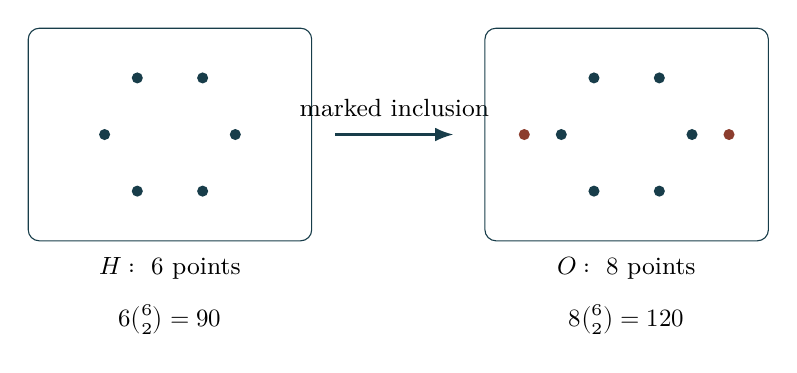
\begin{tikzpicture}[>=Latex,every node/.style={font=\small}]
\draw[rounded corners,draw=ink] (-1.8,-1.35) rectangle (1.8,1.35);
\foreach \a in {0,60,...,300}{
\fill[ink] (\a:0.83) circle(2pt);}
\node at (0,-1.7) {$H:\ 6$ points};
\draw[->,thick,ink] (2.1,0)--(3.6,0);
\node[above] at (2.85,0.1) {marked inclusion};
\draw[rounded corners,draw=ink] (4,-1.35) rectangle (7.6,1.35);
\foreach \a in {0,60,...,300}{
\fill[ink] ($(5.8,0)+(\a:0.83)$) circle(2pt);}
\fill[accent] (4.5,0) circle(2pt);
\fill[accent] (7.1,0) circle(2pt);
\node at (5.8,-1.7) {$O:\ 8$ points};
\node at (0,-2.35) {$6\binom62=90$};
\node at (5.8,-2.35) {$8\binom62=120$};
\end{tikzpicture}
\caption{Marked incidence from six to eight points. The drawing represents
the sets and the inclusion; it does not purport to turn the faces or vertices
of a cube into Steiner blocks without their incidence map.}
\end{figure}

\subsection{The weights precede the pole coefficient}
In the free module of oriented events, the source fixes the
fundamental chain of the turn \cite{precedencia}
\[
c_{12}^{+}=
\sum_{j\in\Z/12\Z}[j,\mathcal F_6]
-[\partial_{\rm ret},\mathcal F_8].
\]
Multiplicity twelve corresponds to the sectors, and multiplicity one
to the oriented seam. The involution changes the orientation of the complete
chain. Let
\[
S_m(q)=\frac{q^m}{1-q^{3m}},\qquad 0<q<1.
\]
The linear reader assigns $S_{90}$ to each sector and $S_{120}$ to the seam;
consequently,
\[
\mathscr R(c_{12}^{+})=12S_{90}-S_{120}.
\]

\begin{theorem}[Pole coefficient and conjugate evaluation]
The image of the fundamental chain has coefficient $1/24$
with respect to $(1-q)^{-1}$ and residue $-1/24$ with respect to $(q-1)^{-1}$.
Its evaluation in the previously generated channels determines
\begin{equation}
\gamma_{\HMT}=
\frac{\pi AC^*}{180}
+12\bigl[S_{90}(q_-)-S_{90}(q_+)\bigr]
-\bigl[S_{120}(q_-)-S_{120}(q_+)\bigr].
\label{eq:gamma}
\end{equation}
\end{theorem}
\begin{proof}
The factorization $1-q^{3m}=(1-q)\sum_{j=0}^{3m-1}q^j$ implies
$\lim_{q\uparrow1}(1-q)S_m(q)=1/(3m)$. By linearity,
\[
\frac{12}{270}-\frac1{360}=\frac1{24}.
\]
The coordinate $q-1$ reverses the sign of the residue.
Conjugate evaluation and the angular component of the source
produce \eqref{eq:gamma}.
\end{proof}

The Diophantine certificate $4a-3b=45$ admits the pairs
$(12+3t,1+4t)$, $t\ge0$; it certifies minimality of $(12,1)$,
but does not replace the origin of the multiplicities in the chain.
The evaluation of \eqref{eq:gamma} is
\[
\gamma_{\HMT}
=0.27400767269445927474725526077398041940\ldots.
\]
This number is an output of the source functional; it is not an external value
used to select $A$, $C^*$, or their coefficients.

\subsection{Parity and structural sensitivity}
Reversing $C^*$ exchanges $q_+$ and $q_-$ and changes the sign
of the angular component. Hence
\[
\gamma_{\HMT}(A,-C^*)=-\gamma_{\HMT}(A,C^*).
\]
The functional preserves orientation, whereas other readers,
such as $q_+q_-$, are even. This difference precedes their physical interpretation.

\subsection{Structural dependence of the functional and area normalization}

The preceding construction places the Barbero--Immirzi parameter at the
meeting of three determinations: marked incidence, dodecaphasic
orientation, and angular evaluation. Incidence supplies the event
spaces; orientation fixes the chain on those spaces;
evaluation transports the chain to a dimensionless quantity. This
decomposition preserves the origin of each coefficient when
the functional is subsequently used in area geometry.

The inclusion \(\mathcal F_6\hookrightarrow\mathcal F_8\) retains
the marked pair of the hexad. Its complement has cardinality
\(2\binom62=30\). This increment reappears as the determinant of the
map reconstructing edge occupations from area and
the weighted observable. Equality of the two integers has a concrete
explanation here: the sector weights differ precisely
by the number of events added by the marked inclusion.

\begin{proposition}[Incidence and recoverability of occupations]
Let \(n_6,n_8\) be the aggregate occupations of two sectors, and let
\(r_6=|\mathcal F_6|\), \(r_8=|\mathcal F_8|\). The map
\[
 (n_6,n_8)\longmapsto(n_6+n_8,r_6n_6+r_8n_8)
\]
is invertible on its image when the inclusion adds at least one
event. For the constructed inclusion, its determinant is 30.
\end{proposition}
\begin{proof}
The matrix of the map is
\(\left(\begin{smallmatrix}1&1\\r_6&r_8\end{smallmatrix}\right)\).
Its determinant is \(r_8-r_6=|\mathcal F_8\setminus\mathcal F_6|\).
The inclusion considered adds \(2\binom62=30\) events. Linear
inversion recovers both occupations and preserves the integer restrictions
of its image.
\end{proof}

The result recovers aggregate occupations. Information about
each link and the order of events remains in the full state
and its additional readers. This hierarchy gives a precise formulation
of the difference between area value and boundary genealogy:
area preserves a sum; the pair of observables preserves the
decomposition of that sum by sectors; the record additionally preserves
its distribution and history.

The parameter \(\gamma_{\HMT}\) transports that incidence to the area
scale. Its structural interpretation is an oriented coefficient
of the hexadic--octadic return functional. The gravitational realization
subsequently recognizes it in the Holst action. Its intrinsic
definition, value, and function in the physical equation are thus distinguished.

\subsection{Structural definition and role of the Barbero--Immirzi parameter}
\label{sec:ii-definicion-barbero}

\begin{definition}[Oriented evaluation of hexadic--octadic incidence]
The parameter \(\gamma_{\HMT}\) is the conjugate evaluation of the
fundamental chain \(c_{12}^{+}\), completed by its angular
component. On the domain \(0<q_\pm<1\), its definition
\eqref{eq:gamma} takes the form
\begin{equation}
 \gamma_{\HMT}
 =\frac{\pi AC^*}{180}
  +[\mathscr R(c_{12}^{+})](q_-)
  -[\mathscr R(c_{12}^{+})](q_+).
 \label{eq:ii-definicion-barbero-evaluacion}
\end{equation}
The marked incidence supplies the event spaces; the oriented
chain fixes their multiplicities; the channels in
\eqref{eq:ii-canales} perform the evaluation.
\end{definition}

The determination jointly uses the cardinalities \(90,120\),
the twelve sector contributions, and the return seam. The
pole coefficient \(1/24\) and Diophantine minimality verify
the compatibility of these weights with the normalization. Their provenance
is preserved in \(c_{12}^{+}\), before the channels are evaluated. Angular
inversion exchanges \(q_+\) and \(q_-\) and produces
\(\gamma_{\HMT}(A,-C^*)=-\gamma_{\HMT}(A,C^*)\): the dimensionless
value transports an orientation of the incidence.

In the geometric realization, this same coefficient enters
\eqref{eq:holst} and the area increment
\(\gamma_{\HMT}a_0\ell_P^2\). The Holst action uses
\(\gamma_{\HMT}\ne0\); the positive areal magnitude uses
\(|\gamma_{\HMT}|\). Proposition~\ref{prop:ii-costura-barbero}
makes the coordinated change of orientation explicit. Thus, the structure
of the parameter explains what it weights in the incidence, what it preserves
under transport, and how it participates in the torsional response and in
the geometric resolution of information.

\clearpage\section{Action ellipse and modular reciprocity}
\label{sec:ellipse}
With the outputs $A,C^*,\hbar>0$ fixed in the chart
$|C^*/A|<1$, we define
\[
\eta_{\rm el}=\operatorname{artanh}(C^*/A),\quad
a_S=\sqrt{2\hbar}\,e^{\eta_{\rm el}/2},\quad
b_S=\sqrt{2\hbar}\,e^{-\eta_{\rm el}/2}.
\]
The balanced canonical coordinates have units of the square root of action;
position and momentum are not added here without a dimensional chart.
The following hold:
\[
a_Sb_S=2\hbar,\qquad
\tau_{\rm el}=i\,\frac{b_S}{a_S},\qquad
R_{\rm el}=\sqrt{\frac{b_S}{a_S}}
=\left(\frac{A-C^*}{A+C^*}\right)^{1/4}.
\]
The positive root determines the composition $\tau_{\rm el}=iR_{\rm el}^2$,
and makes it possible to recover the angular ratio:
\[
\frac{C^*}{A}=\frac{1-R_{\rm el}^4}{1+R_{\rm el}^4}.
\]
Shape inversion sends $R_{\rm el}$ to $R_{\rm el}^{-1}$ and
$\tau_{\rm el}$ to $-1/\tau_{\rm el}$ \cite{elipse}.

\begin{proposition}[Coincident energy, distinguishable action]
Let
\[
D(\eta)=\begin{pmatrix}e^\eta&0\\0&e^{-\eta}\end{pmatrix},
\quad
S_2=\begin{pmatrix}0&1\\1&0\end{pmatrix},
\quad
J_2=\begin{pmatrix}0&-1\\1&0\end{pmatrix}.
\]
Both maps satisfy $T^{\mathsf T}D(-\eta)T=D(\eta)$.
However, for $\omega=\dd Q\wedge\dd P$,
\[
S_2^*\omega=-\omega,\qquad J_2^*\omega=\omega.
\]
If $\mathcal I(\gamma)=\oint_\gamma P\,\dd Q$ on a closed curve,
\[
\mathcal I(S_2\gamma)=-\mathcal I(\gamma),\qquad
\mathcal I(J_2\gamma)=\mathcal I(\gamma).
\]
\end{proposition}
\begin{proof}
Conjugation exchanges the diagonal entries of $D$.
The determinants of $S_2,J_2$ are $-1,1$, respectively, which
proves the transformation of $\omega$. For $\lambda=P\,\dd Q$,
\[
S_2^*\lambda=\dd(PQ)-\lambda,\qquad
J_2^*\lambda=\lambda-\dd(PQ).
\]
Integrating the exact differential over the closed curve completes the proof.
\end{proof}

The quadratic energy and the modulus do not suffice to distinguish the two
transports. The orientation of action does distinguish them, even
in the circular shape. The geometric marking is thus part of the recoverable
reading, not an embellishment added to the value.

% Separate addition: does not replace 07_elipse.tex.
% Provenance: integral 2249, 52.4.1--2, 52.6.2--3, 53.28, and 90.4.6.
% Recovery of results and geometric clarification; local certificate
% verificar_elipse_II.py. Uses no physical radius as a generating input.

\subsection{Semiaxes, foci, and interior radii}
\label{sec:ii-elipse-geometria}

The figure is obtained from the angular and action outputs of the preceding
sections. APP preserves the sheets and their residues and quotients; TRIT fixes
orientation; TPK transports boundary, carry, and memory through to the
representations of the same enriched state and the joint discrete
structure of the continuum. The pair \((A,C^*)\) and the positive section
\(\hbar\) are received here after that construction. The geometry makes explicit
what information their readers preserve, without using an observed length
to select the source state \cite{elipse,hmtedicionintegral}.

Let \(\xi=C^*/A\in(-1,1)\), with \(A\ne0\) and both angles in the
same unit. Write \(\eta=\operatorname{artanh}\xi\) and
\[
 a_S=\sqrt{2\hbar}\,e^{\eta/2},\qquad
 b_S=\sqrt{2\hbar}\,e^{-\eta/2},\qquad
 \gamma(\theta)=(a_S\cos\theta,b_S\sin\theta).
\]
The semiaxes are labeled by their coordinates: if \(\eta<0\),
the vertical axis is the larger. Both belong to the square-root-of-action
line of the balanced chart, not to the line of spatial lengths.

\begin{proposition}[Focal geometry and radial interior]
\label{prop:ii-elipse-focos}
Let \(a=\max(a_S,b_S)\), \(b=\min(a_S,b_S)\). The focal half-distance
and eccentricity are
\begin{equation}
 f_S=\sqrt{a^2-b^2}
 =\sqrt{4\hbar\sinh|\eta|},\qquad
 e_f=\frac{f_S}{a}=\sqrt{1-e^{-2|\eta|}}.
 \label{eq:ii-elipse-focal}
\end{equation}
For \(\eta>0\), the foci are \((\pm f_S,0)\); for
\(\eta<0\), they are \((0,\pm f_S)\). At \(\eta=0\), they coincide with
the center. The boundary radius in polar direction \(\phi\) is
\begin{equation}
 \rho_{\partial}(\phi)
 =\left(\frac{\cos^2\phi}{a_S^2}
        +\frac{\sin^2\phi}{b_S^2}\right)^{-1/2}.
 \label{eq:ii-elipse-radio-polar}
\end{equation}
The interior segment in that direction consists of
\(r(\cos\phi,\sin\phi)\), with \(0\le r<\rho_{\partial}(\phi)\).
In particular, \(b\le\rho_{\partial}(\phi)\le a\).
\end{proposition}

\begin{proof}
The squares of the major and minor semiaxes are
\(2\hbar e^{|\eta|}\) and \(2\hbar e^{-|\eta|}\). Their difference
gives \eqref{eq:ii-elipse-focal}. To verify the focus, suppose
\(\eta>0\). At \(X=\gamma(\theta)\), the distances to
\(F_+=(f_S,0)\) and \(F_-=(-f_S,0)\) satisfy
\[
 |X-F_+|^2=(a_S-f_S\cos\theta)^2,\qquad
 |X-F_-|^2=(a_S+f_S\cos\theta)^2.
\]
Since \(a_S>f_S\), their positive roots sum to \(2a_S\).
For \(\eta<0\), exchanging coordinates gives the same proof.
In the circular case, \(f_S=0\). Finally, substituting
\((Q,P)=r(\cos\phi,\sin\phi)\) into
\(Q^2/a_S^2+P^2/b_S^2=1\) gives
\eqref{eq:ii-elipse-radio-polar}. The coefficient of \(r^2\) lies
between \(a^{-2}\) and \(b^{-2}\), proving the bounds and the
characterization of the interior.
\end{proof}

\subsection{Parametric phase, polar angle, and action area}
\label{sec:ii-elipse-fase-area}

\begin{proposition}[Areal law and two angular coordinates]
\label{prop:ii-elipse-area}
The phase \(\theta\) of \(\gamma\) and its continuous polar angle
\(\phi\), lifted from zero, satisfy
\begin{equation}
 \phi(\theta)=\arg(a_S\cos\theta+i b_S\sin\theta),\qquad
 \frac{d\phi}{d\theta}
 =\frac{a_Sb_S}{a_S^2\cos^2\theta+b_S^2\sin^2\theta}>0.
 \label{eq:ii-elipse-fases}
\end{equation}
In a chart where both tangents are defined,
\(\tan\phi=(b_S/a_S)\tan\theta\). The oriented swept area is
\begin{equation}
 \mathcal A(\theta)=\frac12\int_0^\theta(QP'-PQ')\,dt
 =\hbar\theta,\qquad
 \mathcal A(1)=\hbar,\qquad \mathcal A(2\pi)=h.
 \label{eq:ii-elipse-area-fase}
\end{equation}
\end{proposition}

\begin{proof}
The derivative of the argument of a nonzero vector is
\((QP'-PQ')/(Q^2+P^2)\). Here the numerator is
\(a_Sb_S=2\hbar\), proving the derivative and monotonicity.
The quotient \(P/Q\) gives the tangent relation; the continuous
lift fixes the quadrants and the number of turns. The areal integral
is \(a_Sb_S\theta/2=\hbar\theta\), and
\(h=2\pi\hbar\) gives the final identity.
\end{proof}

Parametric phase does not generally coincide with polar angle. One radian
of phase sweeps \(\hbar\), but is not thereby identified with a circular
arc or a sector of unit polar angle. In polar coordinates,
the same law is written
\(d\mathcal A=\rho_{\partial}(\phi)^2d\phi/2\).
With the orientation of \(\gamma\) used here,
\(\oint P\,dQ=-h\): positive area is \(h\), whereas the
integral of that one-form preserves its sign. This agrees with the
distinction between symplectic and antisymplectic transports in the
preceding section.

\begin{figure}[htbp]
 \centering
 % Computed geometry, not focal coordinates chosen by eye.
% Illustrative algebraic case xi=1/3; not an evaluation of the HMT constants.
\begingroup
\pgfmathsetmacro{\elXi}{1/3}
\pgfmathsetmacro{\elEta}{0.5*ln((1+\elXi)/(1-\elXi))}
\pgfmathsetmacro{\elA}{exp(\elEta/2)}
\pgfmathsetmacro{\elB}{exp(-\elEta/2)}
\pgfmathsetmacro{\elF}{sqrt(\elA*\elA-\elB*\elB)}
\pgfmathsetmacro{\elTheta}{30}
\pgfmathsetmacro{\elX}{\elA*cos(\elTheta)}
\pgfmathsetmacro{\elY}{\elB*sin(\elTheta)}
\pgfmathsetmacro{\elPolar}{atan(\elY/\elX)}
\begin{tikzpicture}[x=2.18cm,y=2.18cm,font=\small,
 every node/.style={inner sep=2pt},>=Stealth]
 \begin{scope}
  \node[font=\bfseries] at (0,1.38) {Shape and orientation};
  \fill[accent!12] (0,0)--(\elA,0)
    plot[domain=0:30,samples=50] ({\elA*cos(\x)},{\elB*sin(\x)})--cycle;
  \draw[ink,thick] (0,0) ellipse[x radius=\elA,y radius=\elB];
  \draw[->,black!55] (-1.42,0)--(1.48,0) node[right]{\(u\)};
  \draw[->,black!55] (0,-1.05)--(0,1.08) node[above]{\(v\)};
  \draw[accent,thick,-{Stealth}] (\elA,0)
    plot[domain=0:30,samples=50] ({\elA*cos(\x)},{\elB*sin(\x)});
  \draw[accent,thick] (0,0)--(\elX,\elY);
  \node[below left,font=\scriptsize] at (0,0) {\(O\)};
  \draw[accent] (.35,0) arc[start angle=0,end angle=\elPolar,radius=.35];
  \node[accent] at (.47,.065) {\(\phi\)};
  \fill[accent] (\elX,\elY) circle[radius=1.4pt];
  \node[above right] at (\elX,\elY) {\(X(\theta)\)};
  \node[accent,align=center,font=\scriptsize] at (1.26,.18) {\(\theta=\pi/6\)};
  \draw[dashed,black!45] (-\elF,0)--(\elX,\elY);
  \draw[dashed,black!45] (\elF,0)--(\elX,\elY);
  \fill[ink] (-\elF,0) circle[radius=1.5pt] node[below]{\(F_-\)};
  \fill[ink] (\elF,0) circle[radius=1.5pt] node[below]{\(F_+\)};
  \draw[<->,black!60] (-\elA,-1.04)--(0,-1.04)
    node[midway,below,font=\scriptsize]{\(a_S/\sqrt{2\hbar}\)};
  \draw[<->,black!60] (-1.32,0)--(-1.32,\elB)
    node[midway,left,font=\scriptsize]{\(\frac{b_S}{\sqrt{2\hbar}}\)};
  \node[align=center,font=\scriptsize] at (0,-1.55)
    {\(\rho_{\partial}(\phi)/\sqrt{2\hbar}=|OX|\)\\
     \(f_S^2=a_S^2-b_S^2\), \quad total area \(h\)};
 \end{scope}
 \begin{scope}[shift={(3.65,0)}]
  \node[font=\bfseries] at (0,1.38) {Reciprocal shape};
  \draw[densely dashed,black!25] (0,0) ellipse[x radius=\elA,y radius=\elB];
  \draw[ink,thick] (0,0) ellipse[x radius=\elB,y radius=\elA];
  \draw[->,black!55] (-1.28,0)--(1.38,0) node[right]{\(u\)};
  \draw[->,black!55] (0,-1.30)--(0,1.26) node[right]{\(v\)};
  \fill[ink] (0,\elF) circle[radius=1.5pt] node[right]{\(F'_+\)};
  \fill[ink] (0,-\elF) circle[radius=1.5pt] node[right]{\(F'_-\)};
  \node[align=center,font=\scriptsize] at (0,-1.55)
    {\(\eta\mapsto-\eta\), \quad \(a_S\leftrightarrow b_S\)\\
     \(R_{\rm el}\mapsto R_{\rm el}^{-1}\), \quad \(a_Sb_S=2\hbar\)};
 \end{scope}
 \draw[->,accent,thick] (1.60,.80)--(2.17,.80)
   node[midway,above,font=\scriptsize]{exchange};
\end{tikzpicture}
\endgroup

 \caption{Semiaxes, foci, and reciprocity of the action ellipse in the
 normalized coordinates \(u=Q/\sqrt{2\hbar}\),
 \(v=P/\sqrt{2\hbar}\). The marked sector has parametric phase
 \(\theta=\pi/6\), different from its polar angle \(\phi\); its action
 area is \(\hbar\pi/6\). The figure uses the algebraic case
 \(\xi=1/3\) to make the relations legible: it does not assign that value
 to the HMT angular output. The foci are computed from the semiaxes.
 On the right, exchanging axes preserves total area \(h\)
 and inverts the dimensionless modular radius.}
 \label{fig:ii-elipse-calculada}
\end{figure}

For the control case of the figure, \(\xi=1/3\), the normalized
coordinates are exactly
\[
 \eta=\tfrac12\log2,\quad
 \frac{a_S}{\sqrt{2\hbar}}=2^{1/4}=1.1892071150\ldots,\quad
 \frac{b_S}{\sqrt{2\hbar}}=
 \frac{f_S}{\sqrt{2\hbar}}=R_{\rm el}=2^{-1/4}=0.8408964153\ldots.
\]
These are regression numbers for the drawing, not values assigned to the angular
generator. The local certificate also checks the circular shape and
the orientations \(\xi=\pm1/3,\pm3/5\).

\subsection{Shape reciprocity and interior distance}

The representation in rectangular coordinates recovers
\begin{equation}
 R_{\rm el}=\sqrt{b_S/a_S}=e^{-\eta/2},\qquad
 R_{\rm el}^4=\frac{1-\xi}{1+\xi},\qquad
 \xi=\frac{1-R_{\rm el}^4}{1+R_{\rm el}^4}.
 \label{eq:ii-elipse-reciproca}
\end{equation}
The proof consists in substituting
\(2\eta=\log((1+\xi)/(1-\xi))\). Exchanging axes
sends \(\eta\) to \(-\eta\), \(R_{\rm el}\) to
\(R_{\rm el}^{-1}\), and \(\tau=iR_{\rm el}^2\) to \(-1/\tau\).
The product \(a_Sb_S\) is preserved. The radius \(R_{\rm el}\) is dimensionless;
the polar radius \(\rho_{\partial}\) has square-root-of-action units.

The interior also admits the Hilbert projective distance. If
\(z_-,x,y,z_+\) are ordered on a chord of the ellipse, define
\[
 d_H(x,y)=\frac12\log
 \frac{|y-z_-|\,|x-z_+|}{|x-z_-|\,|y-z_+|}.
\]
It is a dimensionless distance: the units cancel in the cross-ratio.
The normalization \((Q,P)\mapsto(Q/a_S,P/b_S)\) takes the ellipse
to the unit disk and preserves that ratio, because lengths on a
single line are multiplied by a common factor. It thus transports the metric
to the Beltrami--Klein model. Neither this interior distance nor the distance
between foci is identified with an atomic length.

\subsection{Bohr radius: a consequence of the action scale}
\label{sec:ii-elipse-bohr}

In the electrodynamic realization, the Bohr scale is expressed as
\(a_{\rm B}=\hbar/(m_ec\alpha)\) \cite{codata2022}. In the chain
of the present article, this reading follows the constructions of
action, vacuum, fine structure, and electronic mass. Here
\(\hbar,m_e,c,\alpha>0\) are received in the same dimensional realization.
\begin{proposition}[Areal expression of the Bohr scale]
\label{prop:ii-elipse-bohr}
In that realization,
\begin{equation}
 a_{\rm B}=\frac{a_Sb_S}{2m_ec\alpha}
 =\frac{\mathcal A(2\pi)}{2\pi m_ec\alpha}
 =\frac{\bar\lambda_C(m_e)}{\alpha},\qquad
 \bar\lambda_C(m_e)=\frac{\hbar}{m_ec}.
 \label{eq:ii-elipse-bohr}
\end{equation}
\end{proposition}
\begin{proof}
The identities \(a_Sb_S=2\hbar\) and
\(\mathcal A(2\pi)=2\pi\hbar\), substituted into the Bohr
expression, give the first two members. The definition of
\(\bar\lambda_C(m_e)\) gives the third.
\end{proof}

The numerator has action dimension, and \(m_ec\) has momentum dimension;
the quotient is a length. This composition uses the product of
the semiaxes and the other three quantities: it does not assert that Bohr is a semiaxis,
a focus, a Hilbert distance, or the modular radius. Nor does it equate
electronic mass with the circular quantum of order 108. The notation
\(a_{\rm B}\) avoids confusing this length with the normalization
\(a_0\) of the area operator.

\subsection{Inductive--capacitive realization and constitutive continuity}
\label{sec:ii-elipse-lc}

The electrodynamic bridge of the ellipse preserves an additional chart:
a clock \(\omega>0\) and a reference impedance \(Z_*>0\).
The construction recovered from the corpus defines
\begin{equation}
 L_\eta=\frac{Z_*}{\omega}e^{-\eta},\qquad
 C_\eta=\frac{1}{Z_*\omega}e^\eta,
 \qquad Z_\eta=\sqrt{L_\eta/C_\eta}.
 \label{eq:ii-elipse-lc}
\end{equation}
Here \(C_\eta\) is capacitance, distinct from the counter-angle \(C^*\).
\begin{proposition}[Dynamical product and constitutive quotient]
\label{prop:ii-elipse-lc}
In the preceding chart,
\begin{equation}
 L_\eta C_\eta=\omega^{-2},\qquad
 \frac{Z_\eta}{Z_*}=e^{-\eta}
 =\frac{b_S}{a_S}=R_{\rm el}^{2}.
 \label{eq:ii-elipse-impedancia}
\end{equation}
With \(Q=\sqrt{Z_*}\,q\), \(P=\Phi/\sqrt{Z_*}\), the energy
\(H_{LC}=q^2/(2C_\eta)+\Phi^2/(2L_\eta)\) takes the form
\[
 H_{LC}=\frac\omega2(e^{-\eta}Q^2+e^\eta P^2).
\]
On \(\gamma(\theta)\), its electric and magnetic components are
\(U_E=\hbar\omega\cos^2\theta\) and
\(U_B=\hbar\omega\sin^2\theta\); their sum is \(\hbar\omega\).
\end{proposition}
\begin{proof}
The product in \eqref{eq:ii-elipse-lc} cancels the exponents and
\(Z_*\); the quotient is \(Z_*^2e^{-2\eta}\). Taking the positive
root and using \eqref{eq:ii-elipse-reciproca} gives
\eqref{eq:ii-elipse-impedancia}. Substituting \(q=Q/\sqrt{Z_*}\)
and \(\Phi=\sqrt{Z_*}P\) into \(H_{LC}\) gives its balanced form.
Finally, the semiaxes of \(\gamma\) cancel the factors
\(e^{\mp\eta}\), and \(\cos^2\theta+\sin^2\theta=1\).
\end{proof}

This bridge distinguishes shape, clock, and transducer. The choice
of dynamical direction must agree with the symplectic convention: for
the equations \(\dot Q=\partial_PH\),
\(\dot P=-\partial_QH\), the preceding parametrization satisfies
\(\dot\theta=-\omega\). The energy identities do not depend
on reversing that path.

The vacuum resolvent reader acts on the already produced channels
\(q_\pm=e^{-(A_{\rm rad}\pm C^*_{\rm rad})}\) and incidence
\(90/120\). Its responses
\(r_\pm=(1-q_\pm^{90})/(1-q_\pm^{120})\) give
\(\widehat Z=r_-/r_+\) and \(\widehat c=(r_+r_-)^{-1}\).
These are spectral responses, not geometric radii. Identity
\eqref{eq:ii-elipse-impedancia} fixes the LC realization here;
identifying it with the constitutive vacuum impedance preserves the map
between the two readers and their charts. Their values are not equated merely because
they share the angular antecedent.

% Proposed insertion after 07b_geometria_elipse.tex.
% RESULTADO_RECUPERADO: c52_06_01_incertidumbre.tex, lines 10--91.
% Dependencies: c52_04_01_ley_areal.tex, lines 137--198;
% c52_06_02_intercambio_constitutivo.tex, lines 5--29.
% Local clarification: operator domain, covariance proof,
% reciprocal transport, and the dimensional position--momentum distinction.
% This fragment introduces no additional constant or generator.

\subsection{Canonical covariance and reciprocity of the action ellipse}
\label{sec:ii-area-covarianza}

The preceding construction determines two complementary invariants:
the product of the semiaxes fixes the action area, and their quotient preserves
the anisotropy of the angular pair. We now specify the canonical realization
in which those semiaxes are two standard deviations. The starting
structure is the ellipse already obtained from the angular and action
representations of APP--TRIT--TPK; the operator realization is established
after that construction.

In this subsection we write \(\eta=\eta_{\rm el}
=\operatorname{artanh}(C^*/A)\), with \(|C^*/A|<1\) and
\(\hbar>0\). The angular quotient uses the same unit for its two
components. In the balanced coordinates \((Q,P)\), both having
the dimension of the square root of action, define
\begin{equation}
 V_\eta:=\frac14
 \begin{pmatrix}a_S^2&0\\0&b_S^2\end{pmatrix}
 =\frac{\hbar}{2}
 \begin{pmatrix}e^\eta&0\\0&e^{-\eta}\end{pmatrix}.
 \label{eq:ii-covarianza-geometrica}
\end{equation}
This positive matrix has entries of action dimension. Its interpretation
as quantum covariance is specified by the following realization.

\begin{proposition}[Gaussian realization of action covariance]
\label{prop:ii-covarianza-gaussiana}
Consider the canonical representation on \(L^2(\mathbb R,dQ)\), with
\(\widehat Qf(Q)=Qf(Q)\) and
\(\widehat Pf(Q)=-i\hbar f'(Q)\), initially on the Schwartz
space \(\mathcal S(\mathbb R)\). The normalized state
\begin{equation}
 \psi_\eta(Q)=\bigl(\pi\hbar e^\eta\bigr)^{-1/4}
 \exp\!\left(-\frac{Q^2}{2\hbar e^\eta}\right)
 \label{eq:ii-gaussiana-accion}
\end{equation}
has zero means and covariance matrix \(V_\eta\). In particular,
\begin{equation}
 (\Delta Q)^2=\frac{\hbar e^\eta}{2},\qquad
 (\Delta P)^2=\frac{\hbar e^{-\eta}}{2},\qquad
 \operatorname{Cov}(Q,P)=0,\qquad
 \det V_\eta=\frac{\hbar^2}{4}.
 \label{eq:ii-varianzas-accion}
\end{equation}
This realization saturates the Robertson--Schrödinger inequality.
\end{proposition}

\begin{proof}
The preceding operators are essentially self-adjoint on
\(\mathcal S(\mathbb R)\), which is a common invariant core;
on this space,
\([\widehat Q,\widehat P]=i\hbar I\). For
\(\widehat Y=(\widehat Q,\widehat P)\), the symmetric covariance is
\[
 V_{jk}=\frac12\left\langle
 (\widehat Y_j-\langle\widehat Y_j\rangle)
 (\widehat Y_k-\langle\widehat Y_k\rangle)
 +(\widehat Y_k-\langle\widehat Y_k\rangle)
 (\widehat Y_j-\langle\widehat Y_j\rangle)
 \right\rangle.
\]
With \(s=\hbar e^\eta>0\), let
\(I_s=\int_{\mathbb R}e^{-Q^2/s}\,dQ\). The product of two
equal integrals, evaluated in polar coordinates, gives
\(I_s^2=2\pi\int_0^\infty r e^{-r^2/s}\,dr=\pi s\).
Furthermore, the integral of
\(\frac{d}{dQ}(Qe^{-Q^2/s})\) is zero, by decay at both
ends; hence
\(\int_{\mathbb R}Q^2e^{-Q^2/s}\,dQ=sI_s/2\).
These identities and parity prove normalization, zero mean, and
\(\langle\widehat Q^2\rangle=s/2\). Moreover,
\(\widehat P\psi_\eta=i e^{-\eta}Q\psi_\eta\).
Thus \(\langle\widehat P\rangle=0\),
\(\|\widehat P\psi_\eta\|^2=\hbar e^{-\eta}/2\), and
\(\operatorname{Re}\langle\widehat Q\psi_\eta,
\widehat P\psi_\eta\rangle=0\).

For any normalized state in that domain, Cauchy--Schwarz applied
to \((\widehat Q-\langle\widehat Q\rangle)\psi\) and
\((\widehat P-\langle\widehat P\rangle)\psi\) gives
\[
 (\Delta Q)^2(\Delta P)^2
 \geq \operatorname{Cov}(Q,P)^2
       +\frac14\left|\langle[\widehat Q,\widehat P]\rangle\right|^2
 =\operatorname{Cov}(Q,P)^2+\frac{\hbar^2}{4}.
\]
The computed variances attain equality. Equivalently, the
operator
\[
 a_\eta=\frac{e^{-\eta/2}\widehat Q
                  +i e^{\eta/2}\widehat P}{\sqrt{2\hbar}}
\]
satisfies \([a_\eta,a_\eta^\dagger]=I\) and
\(a_\eta\psi_\eta=0\), by direct substitution.
\end{proof}

\begin{proposition}[Area, dispersion, and reciprocal transport]
\label{prop:ii-area-covarianza-reciprocidad}
The action ellipse is exactly the covariance sublevel set
\begin{equation}
 \mathcal E_\eta
 =\left\{y=(Q,P)^{\mathsf T}:y^{\mathsf T}V_\eta^{-1}y\leq4\right\}
 =\left\{\frac{Q^2}{a_S^2}+\frac{P^2}{b_S^2}\leq1\right\}.
 \label{eq:ii-elipse-covarianza}
\end{equation}
Its area is \(h=2\pi\hbar\), its semiaxes are
\(a_S=2\Delta Q\), \(b_S=2\Delta P\), and
\begin{equation}
 \frac{\Delta P}{\Delta Q}=e^{-\eta}
 =\frac{b_S}{a_S}=R_{\rm el}^2.
 \label{eq:ii-covarianza-forma}
\end{equation}
The canonical rotation \(J_2\) of Section~\ref{sec:ellipse} transports
\(V_\eta\) to \(V_{-\eta}\) and preserves the symplectic form.
\end{proposition}

\begin{proof}
Inverting the diagonal matrix
\eqref{eq:ii-covarianza-geometrica} gives
\eqref{eq:ii-elipse-covarianza}. Its semiaxes are the positive roots of
four times its variances, and
\[
 \operatorname{Area}(\mathcal E_\eta)
 =4\pi\sqrt{\det V_\eta}=2\pi\hbar=h,
\]
in agreement with the areal law~\eqref{eq:ii-elipse-area-fase}.
The ratio of the positive roots proves
\eqref{eq:ii-covarianza-forma}.
If \(M_\eta=\operatorname{diag}(e^{\eta/2},e^{-\eta/2})\), then
\[
 V_\eta=M_\eta V_0M_\eta^{\mathsf T},\qquad
 M_\eta^{\mathsf T}J_2M_\eta=J_2,\qquad
 J_2V_\eta J_2^{\mathsf T}=V_{-\eta}.
\]
These identities follow by multiplication. In operator terms,
\((\widehat Q',\widehat P')=(-\widehat P,\widehat Q)\) preserves
\([\widehat Q',\widehat P']=i\hbar I\). The permutation
\(S_2:(Q,P)\mapsto(P,Q)\) also exchanges the variances but reverses
the sign of the commutator and of the symplectic form. Thus covariance
transport respects the distinction between canonical reciprocity and
orientation reversal already established in Section~\ref{sec:ellipse}.
\end{proof}

\paragraph{Position, momentum, and dimensional transduction.}
Let \(\lambda_{xp}>0\) be a factor of the dimensional chart, with dimension
momentum per unit length. The transformation
\[
 Q=\sqrt{\lambda_{xp}}\,x,\qquad
 P=\frac{p_x}{\sqrt{\lambda_{xp}}}
\]
realizes the balanced pair as a position \(x\) and its conjugate momentum
\(p_x\); it preserves \(dQ\wedge dP=dx\wedge dp_x\) and
\([\widehat x,\widehat p_x]=i\hbar I\). By transformation of
covariance,
\begin{equation}
 V_\eta^{(x,p_x)}=\frac{\hbar}{2}
 \begin{pmatrix}e^\eta/\lambda_{xp}&0\\
                 0&\lambda_{xp}e^{-\eta}\end{pmatrix},\qquad
 \Delta x\,\Delta p_x=\frac{\hbar}{2},\qquad
 \frac{\Delta p_x}{\Delta x}=\lambda_{xp}e^{-\eta}.
 \label{eq:ii-covarianza-dimensiones}
\end{equation}
The dispersion quotient here acquires the dimension momentum per length.
By contrast, \eqref{eq:ii-covarianza-forma} belongs to the balanced chart.
For the inductive--capacitive realization already defined,
\eqref{eq:ii-elipse-impedancia} supplies the dimensionless identity
\(Z_\eta/Z_*=e^{-\eta}=\Delta P/\Delta Q\).
Each reading uses its declared transduction and preserves the same
action determinant.

\paragraph{Contour energy and mean energy of the state.}
The inductive--capacitive realization has Hamiltonian
\[
 H_\eta(Q,P)=\frac{\omega}{2}
 \left(e^{-\eta}Q^2+e^\eta P^2\right),\qquad \omega>0.
\]
On \(\partial\mathcal E_\eta\), its value is
\(H_\eta=\hbar\omega\), by the semiaxis equations. In the
quantum realization of Proposition~\ref{prop:ii-covarianza-gaussiana},
\begin{equation}
 \langle\widehat H_\eta\rangle_{\psi_\eta}
 =\frac{\omega}{2}
 \left(e^{-\eta}\frac{\hbar e^\eta}{2}
       +e^\eta\frac{\hbar e^{-\eta}}{2}\right)
 =\frac{\hbar\omega}{2}.
 \label{eq:ii-energia-contorno-covarianza}
\end{equation}
The two-standard-deviation contour therefore has twice the
mean energy of this Gaussian state. The areal law fixes action
normalization; the angular pair fixes its distribution between the two coordinates;
the canonical representation and explicit state realize that distribution
as covariance. Saturation of uncertainty is thus established in
the realization specified by its operators and its state.

% BEGIN AMPLIACION_MEMORIA_COMPATIBILIDAD_20260922
% Fuente bilingüe común: las fórmulas y pruebas estructurales son idénticas.
\clearpage
\section{\HMTLang{Transporte simpléctico de la elipse de acción}{Symplectic transport of the action ellipse}}
\label{delta22:ii:transporte}
\HMTLang{La elipse previamente construida permite distinguir la medida areal de acción, la anisotropía angular y la tasa de evolución. Esta distinción determina un transporte exacto entre realizaciones elípticas y fija el término de conexión de su expresión hamiltoniana. El antecedente es el par angular publicado por APP--TRIT--TPK, después de la generación regional y de la selección conjunta de \(K\); las operaciones siguientes actúan sobre esas salidas y conservan sus etiquetas de orientación.}{The ellipse constructed above distinguishes the areal measure of action, angular anisotropy, and the rate of evolution. This distinction determines an exact transport between elliptical realizations and fixes the connection term in its Hamiltonian expression. Its antecedent is the angular pair expressed by APP--TRIT--TPK after regional generation and the joint selection of \(K\); the following operations act on those outputs and retain their orientation labels.}

\subsection{\HMTLang{Forma cuadrática y realización inductivo--capacitiva}{Quadratic form and inductive--capacitive realization}}
\HMTLang{Escribimos \(\zeta=\eta_{\rm el}=\operatorname{artanh}(C^*/A)\), con ambas coordenadas angulares en la misma unidad y \(|C^*/A|<1\). El símbolo \(\eta_{\rm ret}\) queda reservado al coeficiente de acción. Para la sección positiva \(\hbar=\eta_{\rm ret}s_0\), \(s_0=10^{-34}\mathcal U_S\), las coordenadas equilibradas de dimensión raíz de acción son}{Write \(\zeta=\eta_{\rm el}=\operatorname{artanh}(C^*/A)\), with both angular coordinates in the same unit and \(|C^*/A|<1\). The symbol \(\eta_{\rm ret}\) is reserved for the action coefficient. For the positive section \(\hbar=\eta_{\rm ret}s_0\), \(s_0=10^{-34}\mathcal U_S\), the balanced coordinates, with the dimension of the square root of action, are}
\[
 Q=\sqrt{2\hbar}\,e^{\zeta/2}\cos\theta,
 \qquad P=\sqrt{2\hbar}\,e^{-\zeta/2}\sin\theta.
\]
\HMTLang{El producto de los semiejes es \(2\hbar\), el área total es \(2\pi\hbar=h\) y el área paramétrica acumulada es \(\hbar\theta\). La fase \(\theta\) es el parámetro de esta representación elíptica. Conservando el transductor \(Z_*>0\) y la frecuencia \(\omega>0\) de la realización anterior, se tiene}{The product of the semiaxes is \(2\hbar\), the total area is \(2\pi\hbar=h\), and the accumulated parametric area is \(\hbar\theta\). The phase \(\theta\) is the parameter of this elliptical representation. Retaining the transducer \(Z_*>0\) and the frequency \(\omega>0\) of the preceding realization gives}
\[
 L_\zeta=\frac{Z_*}{\omega}e^{-\zeta},\qquad
 C_\zeta=\frac{e^\zeta}{Z_*\omega},\qquad
 Q=\sqrt{Z_*}\,q,\quad P=\frac{\Phi}{\sqrt{Z_*}}.
\]
\begin{proposition}[\HMTLang{Composición energética de la elipse}{Energy composition of the ellipse}]
\[
 H_0=\frac{\omega}{2}(e^{-\zeta}Q^2+e^\zeta P^2),\quad
 E_{\rm el}=\hbar\omega\cos^2\theta,\quad
 E_{\rm mag}=\hbar\omega\sin^2\theta.
\]
\HMTLang{Sobre el contorno, \(H_0=E_{\rm el}+E_{\rm mag}=\hbar\omega\).}{On the boundary, \(H_0=E_{\rm el}+E_{\rm mag}=\hbar\omega\).}
\end{proposition}
\begin{proof}
\HMTLang{La sustitución de \(q=Q/\sqrt{Z_*}\), \(\Phi=\sqrt{Z_*}P\) en \(q^2/(2C_\zeta)+\Phi^2/(2L_\zeta)\) produce \(H_0\). Sustituir después la parametrización elíptica da las dos contribuciones y su suma. La acción y la forma preceden al circuito que las realiza.}{Substitution of \(q=Q/\sqrt{Z_*}\), \(\Phi=\sqrt{Z_*}P\) into \(q^2/(2C_\zeta)+\Phi^2/(2L_\zeta)\) yields \(H_0\). Substituting the elliptical parametrization then gives the two contributions and their sum. Action and shape precede the circuit realizing them.}
\end{proof}
\HMTLang{La impedancia de esta realización satisface \(\sqrt{L_\zeta/C_\zeta}/Z_*=e^{-\zeta}\). La impedancia constitutiva del vacío utiliza el cociente de sus lectores \(90/120\); cada impedancia conserva su definición y su transducción.}{The impedance of this realization satisfies \(\sqrt{L_\zeta/C_\zeta}/Z_*=e^{-\zeta}\). The constitutive impedance of the vacuum uses the ratio of its \(90/120\) readers; each impedance retains its definition and transduction.}

\subsection{\HMTLang{Invariante de transporte y conexión hamiltoniana}{Transport invariant and Hamiltonian connection}}
\HMTLang{Sean}{Let}
\[
 S_\zeta=\operatorname{diag}(e^{\zeta/2},e^{-\zeta/2}),\quad
 g_\zeta=S_\zeta^{-\mathsf T}S_\zeta^{-1},\quad
 J_0=\begin{pmatrix}0&-1\\1&0\end{pmatrix},\quad
 R(-\theta)=e^{-\theta J_0}.
\]
\begin{theorem}[\HMTLang{Conservación exacta de la acción cuadrática}{Exact conservation of quadratic action}]
\HMTLang{Para una sucesión de formas \(\zeta_n\) y fases \(\theta_n\), el transporte}{For a sequence of shapes \(\zeta_n\) and phases \(\theta_n\), the transport}
\[
 X_{n+1}=T_nX_n,\qquad
 T_n=S_{\zeta_{n+1}}R(-\theta_n)S_{\zeta_n}^{-1}
\]
\HMTLang{tiene determinante uno y conserva}{has determinant one and preserves}
\[
 I_n=\tfrac12X_n^{\mathsf T}g_{\zeta_n}X_n,
 \qquad T_n^{\mathsf T}g_{\zeta_{n+1}}T_n=g_{\zeta_n}.
\]
\end{theorem}
\begin{proof}
\HMTLang{Los determinantes de \(S_\zeta\) y \(R\) son uno. En el producto cuadrático, los factores \(S_{\zeta_{n+1}}\) cancelan sus inversos; \(R^{\mathsf T}R=I\) deja \(S_{\zeta_n}^{-\mathsf T}S_{\zeta_n}^{-1}\). Esta identidad prueba la conservación para cada paso y, por composición, para cualquier longitud. Una sucesión publicada por una ruta TPK se transporta con esa ruta y sus etiquetas.}{The determinants of \(S_\zeta\) and \(R\) are one. In the quadratic product, the factors \(S_{\zeta_{n+1}}\) cancel their inverses; \(R^{\mathsf T}R=I\) leaves \(S_{\zeta_n}^{-\mathsf T}S_{\zeta_n}^{-1}\). This identity proves conservation at every step and, by composition, at any length. A sequence expressed by a TPK route is transported together with that route and its labels.}
\end{proof}
\begin{theorem}[\HMTLang{Generador diferenciable y término mixto}{Differentiable generator and mixed term}]
\HMTLang{Si \(\zeta\) es de clase \(C^1\), \(\omega>0\) es continua y \(X=S_\zeta Y\), \(\dot Y=-\omega J_0Y\), entonces}{If \(\zeta\) is \(C^1\), \(\omega>0\) is continuous, and \(X=S_\zeta Y\), \(\dot Y=-\omega J_0Y\), then}
\[
 \dot Q=\tfrac12\dot\zeta Q+\omega e^\zeta P,
 \qquad \dot P=-\omega e^{-\zeta}Q-\tfrac12\dot\zeta P.
\]
\HMTLang{Con la convención \(\dot Q=\partial_PH\), \(\dot P=-\partial_QH\), su Hamiltoniano, salvo un sumando dependiente del tiempo, es}{With the convention \(\dot Q=\partial_PH\), \(\dot P=-\partial_QH\), its Hamiltonian, up to an additive function of time, is}
\begin{equation}
 H_{\rm tot}=\frac\omega2(e^{-\zeta}Q^2+e^\zeta P^2)
             +\frac{\dot\zeta}{2}QP.
 \label{delta22:ii:hamiltoniano}
\end{equation}
\HMTLang{El invariante \(I=(e^{-\zeta}Q^2+e^\zeta P^2)/2\) se conserva exactamente.}{The invariant \(I=(e^{-\zeta}Q^2+e^\zeta P^2)/2\) is conserved exactly.}
\end{theorem}
\begin{proof}
\HMTLang{Derivar \(X=S_\zeta Y\) produce \(\dot S_\zeta S_\zeta^{-1}=\operatorname{diag}(\dot\zeta/2,-\dot\zeta/2)\) y el término rotacional conjugado. Las derivadas parciales de \eqref{delta22:ii:hamiltoniano} reproducen las dos ecuaciones. En \(\dot I\), las contribuciones explícitas \(-\dot\zeta e^{-\zeta}Q^2/2+\dot\zeta e^\zeta P^2/2\) cancelan las procedentes de la diagonal del generador; los términos cruzados rotacionales se anulan entre sí.}{Differentiating \(X=S_\zeta Y\) yields \(\dot S_\zeta S_\zeta^{-1}=\operatorname{diag}(\dot\zeta/2,-\dot\zeta/2)\) and the conjugated rotational term. The partial derivatives of \eqref{delta22:ii:hamiltoniano} reproduce both equations. In \(\dot I\), the explicit contributions \(-\dot\zeta e^{-\zeta}Q^2/2+\dot\zeta e^\zeta P^2/2\) cancel those from the diagonal of the generator; the rotational cross terms cancel each other.}
\end{proof}
\HMTLang{En la parametrización elíptica, \(QP=I\sin2\theta\) y \(\dot\theta=-\omega\). Por tanto \(H_{\rm tot}=I\omega+(I\dot\zeta/2)\sin2\theta\). La matriz cuadrática tiene determinante \(\omega^2-\dot\zeta^2/4\): es definida positiva exactamente para \(|\dot\zeta|<2\omega\), y semidefinida positiva en igualdad. La conservación de \(I\) y la dependencia temporal de \(H_{\rm tot}\) expresan propiedades distintas. Como control algebraico, omitir el término mixto produce \(\dot I=\dot\zeta(e^\zeta P^2-e^{-\zeta}Q^2)/2\). En la representación cuántica correspondiente, la expresión simétrica del término mixto es \(\dot\zeta(\widehat Q\widehat P+\widehat P\widehat Q)/4\).}{In the elliptical parametrization, \(QP=I\sin2\theta\) and \(\dot\theta=-\omega\). Thus \(H_{\rm tot}=I\omega+(I\dot\zeta/2)\sin2\theta\). The quadratic matrix has determinant \(\omega^2-\dot\zeta^2/4\): it is positive definite precisely when \(|\dot\zeta|<2\omega\), and positive semidefinite at equality. Conservation of \(I\) and time dependence of \(H_{\rm tot}\) express different properties. As an algebraic control, omitting the mixed term gives \(\dot I=\dot\zeta(e^\zeta P^2-e^{-\zeta}Q^2)/2\). In the corresponding quantum representation, the symmetric mixed term is \(\dot\zeta(\widehat Q\widehat P+\widehat P\widehat Q)/4\).}

\subsection{\HMTLang{Compatibilidad genealógica y transporte conformemente simpléctico}{Genealogical compatibility and conformally symplectic transport}}
\HMTLang{En la sección generada,}{On the generated section,}
\[
 \zeta=\operatorname{artanh}\frac{2(\eta_{\rm ret}+\alpha)}{1000\alpha}.
\]
\HMTLang{Fijar \(\alpha\) y \(\eta_{\rm ret}\) fija la forma. La versión variable del teorema describe el transporte entre formas admitidas; su realización dinámica conserva la actualización que determina esas formas. Para secciones positivas \(\hbar_n\) en una misma carta dimensional, sea \(\rho_n=\hbar_{n+1}/\hbar_n\). Entonces}{Fixing \(\alpha\) and \(\eta_{\rm ret}\) fixes the shape. The variable version of the theorem describes transport between admissible shapes; its dynamical realization retains the update determining those shapes. For positive sections \(\hbar_n\) in the same dimensional chart, let \(\rho_n=\hbar_{n+1}/\hbar_n\). Then}
\[
 \widetilde T_n=\sqrt{\rho_n}\,T_n,\quad
 \det\widetilde T_n=\rho_n,\quad
 \widetilde T_n^{\mathsf T}g_{\zeta_{n+1}}\widetilde T_n
 =\rho_ng_{\zeta_n},\quad
 \frac{I_{n+1}}{\hbar_{n+1}}=\frac{I_n}{\hbar_n}.
\]
\HMTLang{Estas igualdades se deducen multiplicando el transporte anterior por \(\sqrt{\rho_n}\). La forma simpléctica y la acción normalizada se transportan conjuntamente. El límite diferenciable tiene traza \(\dot\hbar/\hbar\); en una forma simpléctica fija, un generador hamiltoniano lineal tiene traza cero. Por ello, la sección variable exige conservar la forma transportada o los grados de libertad que intercambian acción. Si la variación es un cambio de unidades, se transportan primero las bases dimensionales.}{These equalities follow by multiplying the preceding transport by \(\sqrt{\rho_n}\). The symplectic form and normalized action are transported together. The differentiable limit has trace \(\dot\hbar/\hbar\); for a fixed symplectic form, a linear Hamiltonian generator has zero trace. A variable section therefore requires retaining the transported form or the degrees of freedom exchanging action. If the variation is a change of units, the dimensional bases are transported first.}

\HMTLang{La distinción operacional es precisa. Bajo un cambio pasivo \(X=S_\zeta Y\), también el lector satisface \(L_X(S_\zeta Y)=L_Y(Y)\); el término mixto representa la conexión de coordenadas. Una deformación física se especifica mediante la evolución relativa entre sistema y referencia, obtenida de sus actualizaciones y leída con el mismo dispositivo. Una atribución energética incorpora el campo, el registro y el controlador. Así quedan separadas la conservación demostrada de la acción cuadrática, la realización hamiltoniana y las condiciones de una respuesta física contrastable.}{The operational distinction is precise. Under a passive change \(X=S_\zeta Y\), the reader also satisfies \(L_X(S_\zeta Y)=L_Y(Y)\); the mixed term represents the coordinate connection. A physical deformation is specified by relative evolution between system and reference, obtained from their updates and read with the same device. An energy attribution includes the field, the record, and the controller. This separates the proved conservation of quadratic action, its Hamiltonian realization, and the conditions for a testable physical response.}

% END AMPLIACION_MEMORIA_COMPATIBILIDAD_20260922
\clearpage% Self-contained fragment for the draft of article II, September 8, 2026.
% Provenance: RESULTADO_RECUPERADO and FORMALIZACION_REUNIDA from the owners
% B07/c41_ckm.tex and C02/74_mezcla_contenido_exclusivo_post_rev2.tex in
% BORRADOR_02; integral 2249, chaps. 49, 92.6, 92.24, and 93.10--93.11.
% The originals and their complete proof support are neither replaced nor edited.
% Bibliographic keys used: ckm, mezcla, pmnsespectral, cpt.
% Requires: amsmath, amssymb, amsthm; theorem/proposition/definition/remark.

\section{CKM mixing angles, CP phase, and leptonic transport}
\label{sec:ii-propagacion-angular}

\subsection{Common antecedent and separation of the two transports}

The article's common foundation produces the enriched state through
the two APP evaluations, the oriented selection of TRIT, and the
effective composition of selection, transport, carry, memory, and return
in TPK. Angular representations do not replace that state: they are readers
of its record. In particular, the prolongation
\(w_6\to w_{12}\to w_{18}\to w_{24}\to w_{30}\to R_{36}\to G_9\)
preserves the provenance of the numerical readings, and the holonomy
\(\Gamma_9\) acts before the reduced representation \(K_{\rm ph}\).
Phase return does not restart the record.

Two classes of objects are received here from that same antecedent. The first
contains the direct angle, the counter-angle, and the torsional defect
\(\Delta_4\), already constructed through their own readers. The second contains
the surviving extensions, their observable routes, the dodecaphasic
record, and the operators of the material fibers. The
extension--route--record--signature--character--towers chain preserves the atlas
\(81/56/13/324\) and distinguishes the null chart from the positive branch.
The mixing angles do not retrospectively choose those routes or generate
the mass eigenvalues.

Quark transport uses a rational angular chart and its complex
unitary realization. Leptonic transport uses the spectral frames
of the charged and neutral fibers. Both come from the common discrete
structure, but their domains, readers, and changes of basis are distinct.
The Barbero--Immirzi functional and mixing are not defined by one
another either: they receive typed representations of the angular and incidence antecedent.
Their relationship is expressed through those maps, not through a
retrospective formula using a Barbero value as a mixing selector.

\begin{remark}[Sectorial rules and evaluation of the reader]
The three sectorial rules and their evaluation are developed below
in Section~\ref{sec:ii09-construccion-sectorial}. Theorem
\ref{thm:ii09-matriz-sectorial} obtains the columns as images of the
angular basis. Subsequent proofs establish inversion of the chart,
sheet transport, the metric, and the complex realization.
The choice of rules and evaluation of their coefficients are two
distinct mathematical questions: the starting system is declared in
Definition~\ref{def:ii09-sistema-sectorial}, and the theorem's proof
uses that complete system. The preceding composition that selects those
rules from incidence requires its own proof.
\end{remark}

% Separate contribution, 9 September 2026.
% RESULTADO_RECUPERADO: sectorial construction from source 08_ckm_cp.tex.
% FORMALIZACION_REUNIDA: parity decomposition and representational compatibility.
% Insert before the rational CKM chart; retain the subsequent development.
% Provenance and exact scope are in 08b_procedencia_angular.md.

\subsection{Sectorial incidence and construction of the angular reader}
\label{sec:ii09-construccion-sectorial}

The angular construction uses the action and closure representations
previously obtained from APP--TRIT--TPK. The direct angle,
counter-angle, and torsional defect preserve their own domains.
The quark reader combines these three coordinates through sectorial
incidence; its evaluation precedes complex amplitudes and
metrological comparison. Hexadic--octadic inclusion enters
the third sector through the difference of its cardinalities.

% ARQUITECTURA_AUTORAL_PREEXISTENTE: bidirectional half-square of N42.
% FORMALIZACION_NUEVA: pair groupoid and stabilizer weighting.
\subsubsection{Marked incidence and bidirectional normalization}
\label{sec:ii09-normalizacion-bidireccional}

The reader invariants preserve the nature of the object from which
they arise. The marked intersection $B_K=H_e\cap P_\pi$ has cardinality
$b=4$; the integer $q=7$ is the coordinate of the pivot $p_\varphi$ in
the oriented numbering. The determination order of the Steiner
design is $p=5$. The hexadic and octadic supports have cardinalities $h_6=6$
and $o_8=8$, and the tritic orientation alphabet has cardinality $t=3$.
A support cardinality and a pivot coordinate are used through
their respective maps, even when both are expressed as integers.

Normalization of the pentagonal self-crossing admits the following
explicit realization. Let $P$ be the five-position support of the closure,
and let $X=P\times P$ be its space of ordered pairs. Bidirectional
inversion on this space is
\[
 \jmath:X\longrightarrow X,\qquad \jmath(x,y)=(y,x),
 \qquad\jmath^2=I.
\]
The stabilizer information of each orbit is preserved. For an
orbit $[z]$, define its weight as
$1/|\operatorname{Stab}_{C_2}(z)|$. The sum of these weights is the
cardinality of the action groupoid $X/\!/C_2$.

\begin{proposition}[Orbital measure of bidirectional self-crossing]
\label{prop:ii09-semicuadrado-orbital}
For a finite support of cardinality $p$, inversion of ordered pairs
determines
\[
 |(P\times P)/\!/C_2|
 =\sum_{[z]\in(P\times P)/C_2}
      \frac1{|\operatorname{Stab}_{C_2}(z)|}
 =\frac{p^2}{2}.
\]
For $p=5$, the self-crossing has ten free orbits and five fixed
orbits, and its orbital measure is $10+5/2=25/2$.
\end{proposition}
\begin{proof}
Each diagonal pair $(x,x)$ forms a fixed orbit, whose stabilizer
has order two; there are $p$ such orbits. The remaining $p(p-1)$ pairs
are grouped in twos, with trivial stabilizer. Their contribution is
therefore $p(p-1)/2$, and that of the diagonal is $p/2$. The sum is
$p^2/2$. Equivalently, the orbit--stabilizer identity gives
$1/|\operatorname{Stab}(z)|=|[z]|/2$; summing over all orbits
produces $|P\times P|/2$.
\end{proof}

The measure explicitly preserves the contribution of fixed points.
The ordinary orbit set has cardinality $p(p+1)/2$, equal to
fifteen in the pentagonal closure. The orbital measure and that cardinality
are two determinate readings of the same inversion. The reader's
bidirectional normalization uses the former: the ten free orbits
have unit weight, and the five diagonals have half-unit weight.

This realization specifies the factor $p^2/2$ used in the following
sectorial system. The assignment of that contribution to sector $23$,
its negative orientation, and the other two incidence rules remain
specified by the complete sectorial system. The proof establishes the
normalization of self-crossing and preserves the selection of the
angular functionals as a distinct matter.


% FORMALIZACION_NUEVA of the lift of N39, compatible with (rho9,q9),
% T_d and Upd_t; preexisting remainder/quotient and orientation architecture.
% Separate research fragment. Does not select the CKM N42 rules.
\subsubsection{Carry transport and integer holonomy of the arithmetic crossing}
\label{subsec:transporte-entero-cruce}

The modular reading of the crossing admits an integral realization retaining
the information accumulated while crossing the edge. This realization
is developed here through transport quotients. Its domain is a lifted
chart of the APP support; the subsequent assignment of a region to an angular
sector retains its own incidence map.

\paragraph{Nonadic chart and lifted transport.}
We use the exact decomposition
\[
 \rho_9(n)=1+((n-1)\bmod9),\qquad
 q_9(n)=\left\lfloor\frac{n-1}{9}\right\rfloor,
 \qquad n=\rho_9(n)+9q_9(n).
\]
A lifted position is
$z=(x,y,q_x,q_y)\in D_9^2\times\mathbb Z^2$, where
$X=x+9q_x$ and $Y=y+9q_y$. The integer increment $u$ of the first
coordinate acts by
\[
 T^x_u(x,y,q_x,q_y)=
 \bigl(\rho_9(x+u),y,q_x+c_9(x;u),q_y\bigr),\qquad
 c_9(x;u)=\left\lfloor\frac{x+u-1}{9}\right\rfloor.
\]
The second coordinate is transported in the same way. Cardinal
advances correspond to $u=\pm1$; the zero increment preserves the state.
The cocycle satisfies
\[
 c_9(x;u+v)=c_9(x;u)+c_9(\rho_9(x+u);v).
\]
Indeed, both sides are the quotient of the unique decomposition of
$x+u+v$ with remainder in $D_9$. Consequently,
$T^x_vT^x_u=T^x_{u+v}$ and $T^x_{-u}=(T^x_u)^{-1}$; the transports
of the two coordinates commute. The state preserves the number of edge
crossings even when the visible position returns.

\paragraph{Lifted sheets and update of records.}
The integral realization is fixed by prolonging the APP arithmetic
operations to the transported coordinates:
\begin{align*}
 \widetilde S(z)&=X+Y=x+y+9(q_x+q_y),\\
 \widetilde P(z)&=XY
 =xy+9(q_xy+q_yx)+81q_xq_y.
\end{align*}
At each position the record of both sheets is preserved:
\[
 \bigl(\rho_9(\widetilde S),q_9(\widetilde S),
       \rho_9(\widetilde P),q_9(\widetilde P)\bigr).
\]
If $e:z\to z'$ is a link and $T$ the selected sheet, its full increment
is obtained from the record before and after transport:
\begin{equation}
 \delta_e\widetilde T=
 \rho_9(\widetilde T(z'))-\rho_9(\widetilde T(z))
 +9\bigl(q_9(\widetilde T(z'))-q_9(\widetilde T(z))\bigr).
 \label{eq:cruce-incremento-registro}
\end{equation}
This identity makes preservation explicit: the residue jump and
quotient increment together reconstruct the variation of the sheet.
Sheet selection, cardinal transport, and record
update are distinct operations. In this chart, the ordered sheet
selection $(T_x,T_y)$ is first composed with $T_d$ and the update
of its quotients; the formula does not postulate that the entire TPK is reduced
to this local representation.

\begin{proposition}[Integral curvature and boundary transport]
\label{prop:cruce-stokes-integral}
Define
$\widetilde A_x=\delta_x\widetilde T_x$ and
$\widetilde A_y=\delta_y\widetilde T_y$ through
\eqref{eq:cruce-incremento-registro}, and let
\[
 \widetilde F_{xy}(X,Y)=
 \widetilde A_x(X,Y)+\widetilde A_y(X+1,Y)
 -\widetilde A_x(X,Y+1)-\widetilde A_y(X,Y).
\]
Homogeneous choices have zero curvature. The mixed choices
$(\widetilde S,\widetilde P)$ and
$(\widetilde P,\widetilde S)$ have curvature
$+1$ and $-1$, respectively, as integers. For the positive boundary of a rectangle
$R_{a,b}$ with integer sides $a,b>0$,
\[
 \widetilde W_{SP}(\partial R_{a,b})=ab,\qquad
 \widetilde W_{PS}(\partial R_{a,b})=-ab.
\]
The result is independent of the base point and the number of crossings
of nonadic seams.
\end{proposition}

\begin{proof}
Exact reconstruction of the two sheets gives
\[
 \delta_x\widetilde S=\delta_y\widetilde S=1,
 \qquad\delta_x\widetilde P=Y,
 \qquad\delta_y\widetilde P=X.
\]
Thus the $SP$ connection is $(1,X)$, with curvature
$1+(X+1)-1-X=1$; the $PS$ connection is $(Y,1)$, with curvature
$Y+1-(Y+1)-1=-1$. For a single sheet, mixed
differences cancel. Summing the curvatures of the $ab$ plaquettes cancels each
interior link with its inverse and preserves the boundary links.
This yields $\pm ab$ in $\mathbb Z$. The transported quotients
ensure the same identity holds across any seam.
\end{proof}

The boundary accumulator can in turn be retained in nonadic form:
$W=r_W+9q_W$. For an integer contribution $w_e$, it is updated by
\[
 r_W'=\rho_9(r_W+w_e),\qquad
 q_W'=q_W+\left\lfloor\frac{r_W+w_e-1}{9}\right\rfloor.
\]
Composition by links provides the same sum as direct integer
evaluation. In this chart, integer zero has coordinates
$(r_W,q_W)=(9,-1)$; this is an arithmetic representation of the accumulator,
without further identification with the distinct oriented zeros of TRIT.

\paragraph{Three operations on orientation.}
Let $\gamma$ be a closed cardinal route. Its time reversal
$\gamma^{-1}$ reverses the order of links and the orientation of each;
by additivity,
\[
 \widetilde W_{SP}(\gamma^{-1})=-\widetilde W_{SP}(\gamma).
\]
Exchange of sheets likewise satisfies
\[
 \widetilde W_{PS}(\gamma)=-\widetilde W_{SP}(\gamma).
\]
To check this on any route, note that the sum of both
connections is the exact increment of
$\widetilde S+\widetilde P=X+Y+XY$; its integral over a loop is zero.

The simultaneous half-turn of both directions, on the other hand, acts
through $J_c(X,Y)=(2c_x-X,2c_y-Y)$, with $2c\in\mathbb Z^2$,
so that it preserves the lattice chart. For a loop,
\[
 \widetilde W_{SP}(J_c\gamma)=\widetilde W_{SP}(\gamma).
\]
Indeed, the closed horizontal contribution is zero, and the vertical one
transforms as
$\sum (2c_x-X)(-\delta Y)=\sum X\delta Y$, since
$\sum\delta Y=0$. A spatial half-turn therefore preserves the
area orientation of this chart. Its combination with time reversal
or sheet exchange is computed by composing the corresponding
operations.

The difference matters for the electronic record: simultaneous reversal
of both displacements every $27$ advances produces, in
windows of $9$, the sequence
\[
 \tau_j=(-1)^{\lfloor j/3\rfloor},\qquad 0\leq j<12,
 \qquad (+,+,+,-,-,-,+,+,+,-,-,-).
\]
This sequence records advance orientations. Holonomy additionally requires
the links traversed, selected sheets, and accumulated
quotients. Transport of electronic orientation is thus preserved
without identifying a half-turn of both axes with time reversal
of a loop.

\paragraph{Application to the marked crossing and sector scope.}
For the rectangular crossing with sides $4$ and $7$, this realization evaluates
exactly
\[
 \widetilde W_{SP}=28=1+9\cdot3,\qquad
 \widetilde W_{SP}(\gamma^{-1})=-28=8+9(-4).
\]
The integer preserves the oriented area; the isolated remainder represents only
its nonadic class. For example, from $(7,1)$ the periodic
representatives of the links sum to $-35$, whereas the carry correction
adds $63$ and recovers $28$.

In the marked incidence of the angular reader, $4$ is
$|H_e\cap P_\pi|$ and $7$ is the marked pivot $p_\varphi$.
The rectangular reading supplies an integer realization of the product
$|H_e\cap P_\pi|\,p_\varphi$ once that crossing has been declared. The
map identifying that region with sector $12$ must preserve
the mark and orientation of the sector system in
Definition~\ref{def:ii09-sistema-sectorial}. Sector assignments
$12,23,13$ and their combinations of $A,h,\Delta^\circ$
are an additional specification beyond the rectangular-holonomy law.
The present result makes the area lift, carry, and
their involutions explicit, with these starting data declared.


\begin{definition}[Sectorial system of angular incidence]
\label{def:ii09-sistema-sectorial}
The sectorial system consists of the ordered sextuple of invariants
\[
 (b,p,q,h_6,o_8,t)=(4,5,7,6,8,3)
\]
and the linear maps, on angular coordinates
\((a,u,d)\),
\begin{align}
 \mathscr A_{12}^{\rm ang}(a,u,d)&=2a-pu+bq\,d,\label{eq:ii09-sector12}\\
 \mathscr A_{23}^{\rm ang}(a,u,d)&=qu-\frac{p^2}{2}\,d,\label{eq:ii09-sector23}\\
 \mathscr A_{13}^{\rm ang}(a,u,d)&=a-pb\,u-\frac{o_8-h_6}{t}\,d.
 \label{eq:ii09-sector13}
\end{align}
The symbols \(h_6,o_8\) preserve the cardinalities of the marked
incidence; \(t=3\) is the declared tritic normalization of that sector.
The sextuple and the three rules jointly form the starting
system of this construction.
\end{definition}

\begin{theorem}[Exact evaluation of the sectorial system]
\label{thm:ii09-matriz-sectorial}
The joint map
\((\mathscr A_{12}^{\rm ang},\mathscr A_{23}^{\rm ang},
\mathscr A_{13}^{\rm ang})^{\mathsf T}\) of
Definition~\ref{def:ii09-sistema-sectorial} has the unique matrix
\[
 \mathsf M_{\rm CKM}=
 \begin{pmatrix}
 2&-5&28\\
 0&7&-25/2\\
 1&-20&-2/3
 \end{pmatrix}.
\]
The three columns are the images of the coordinate vectors
\((1,0,0)\), \((0,1,0)\), and \((0,0,1)\) under these maps.
\end{theorem}
\begin{proof}
The sectorial operations give
\[
 bq=4\cdot7=28,\qquad p^2/2=5^2/2=25/2,
 \qquad pb=5\cdot4=20,\qquad
 (o_8-h_6)/t=(8-6)/3=2/3.
\]
Thus the successive images of the coordinate basis are
\[
 c_A=(2,0,1)^{\mathsf T},\qquad
 c_h=(-5,7,-20)^{\mathsf T},\qquad
 c_\Delta=(28,-25/2,-2/3)^{\mathsf T}.
\]
A linear map is determined by its images on a
basis. The matrix with these images as its columns is the one indicated.
The proof uses the complete sectorial system of the definition.
\end{proof}

On the previously produced coordinates, take
\[
 (a,u,d)=\left(A_{\deg},\frac{C^*_{\deg}}6,
                       \frac{180}{\pi}\Delta_4\right).
\]
The direct, conjugate, and torsional contributions to each angle
are thereby individualized. In particular, the difference
\(o_8-h_6=2\) is preserved in the coefficient of the torsional
defect in sector \(13\). This concrete presence makes it possible to follow
incidence through to the angular reader, keeping the sectorial
system, its evaluation, and the unitary parametrization separate.


\subsection{Rational CKM chart and angular units}

We write \(A_{\rm deg}\) and \(C^*_{\rm deg}\) for the coordinates in
degrees of the HMT angles already generated. We use the abbreviations
\begin{equation}
 h_\theta=\frac{C^*_{\rm deg}}6,
 \qquad
 \Delta_{\rm deg}=\frac{180}{\pi_{\rm HMT}}\Delta_4,
 \qquad
 x_\theta=(A_{\rm deg},h_\theta,\Delta_{\rm deg})^{\mathsf T}.
 \label{eq:ii-angular-chart}
\end{equation}
Here, \(h_\theta\) is an angular coordinate, distinct from the Planck
constant \(h\). Conversion to degrees is a subsequent change of coordinates; it
does not introduce a conventional value of \(\pi\) into the generator.

\begin{definition}[Quark angular reader]
The inherited reader \(\mathsf M_{\rm CKM}:\mathbb R^3\to\mathbb R^3\)
evaluates the coordinates
\begin{equation}
 \boldsymbol\theta_{\rm deg}=\mathsf M_{\rm CKM}x_\theta,
 \qquad
 \mathsf M_{\rm CKM}=
 \begin{pmatrix}
 2&-5&28\\
 0&7&-25/2\\
 1&-20&-2/3
 \end{pmatrix},
 \qquad
 \delta_{\rm deg}=9A_{\rm deg}.
 \label{eq:ii-ckm-map}
\end{equation}
The component order is \((12,23,13)\). Subsequent trigonometric
functions are evaluated at
\(\vartheta_{ab}=(\pi_{\rm HMT}/180)\theta_{ab,\rm deg}\) and
\(\delta=(\pi_{\rm HMT}/180)\delta_{\rm deg}\).
\end{definition}

\begin{proposition}[Rational reconstruction of the coordinates]
The reader has determinant \(-3857/6\) and inverse
\begin{equation}
 \mathsf M_{\rm CKM}^{-1}=
 \begin{pmatrix}
 1528/3857&3380/3857&801/3857\\
 75/3857&176/3857&-150/3857\\
 6/551&-30/551&-12/551
 \end{pmatrix}.
 \label{eq:ii-ckm-inverse}
\end{equation}
In particular,
\begin{align}
 A_{\rm deg}
 &=\frac{1528\theta_{12,\rm deg}+3380\theta_{23,\rm deg}
          +801\theta_{13,\rm deg}}{3857},\nonumber\\
 C^*_{\rm deg}
 &=\frac{6(75\theta_{12,\rm deg}+176\theta_{23,\rm deg}
          -150\theta_{13,\rm deg})}{3857},\nonumber\\
 \Delta_{\rm deg}
 &=\frac{6\theta_{12,\rm deg}-30\theta_{23,\rm deg}
          -12\theta_{13,\rm deg}}{551}.
 \label{eq:ii-ckm-recover}
\end{align}
The phase satisfies the exact linear check
\begin{equation}
 3857\delta_{\rm deg}
 =9(1528\theta_{12,\rm deg}+3380\theta_{23,\rm deg}
      +801\theta_{13,\rm deg}).
 \label{eq:ii-ckm-phase-check}
\end{equation}
\end{proposition}

\begin{proof}
Expansion of the determinant in \eqref{eq:ii-ckm-map} gives
\(-3857/6\). Multiplying the matrix given in
\eqref{eq:ii-ckm-inverse} by \(\mathsf M_{\rm CKM}\), in either
order, gives \(I_3\). Its rows recover the three components of
\(x_\theta\); the second is multiplied by six to recover
\(C^*_{\rm deg}\). Finally, we use
\(\delta_{\rm deg}=9A_{\rm deg}\).
\end{proof}

Inversion reconstructs the reader's coordinates once the reader is fixed. It does not
turn observed angles into antecedents of \(A\), \(C^*\), or
\(\Delta_4\).

\subsection{Geometric decomposition under sheet inversion}
\label{sec:ii09-descomposicion-paridad}

In the angular chart, sheet inversion preserves \(a,d\) and
reverses \(u\). The expressed vector admits the decomposition
\[
 \boldsymbol\theta_+=a c_A+u c_h+d c_\Delta,
 \qquad
 \boldsymbol\theta_-=a c_A-u c_h+d c_\Delta.
\]
\begin{proposition}[Even and odd components of angular transport]
\label{prop:ii09-paridad-angular}
The two vectors satisfy
\[
 \frac{\boldsymbol\theta_++\boldsymbol\theta_-}{2}
       =a c_A+d c_\Delta,\qquad
 \frac{\boldsymbol\theta_+-\boldsymbol\theta_-}{2}=u c_h.
\]
The contribution that changes sign occupies the line
\(\operatorname{span}(c_h)\); the preserved component occupies
\(\operatorname{span}(c_A,c_\Delta)\).
\end{proposition}
\begin{proof}
The sum cancels the terms \(u c_h\), and the difference cancels
the other two. The columns are linearly independent, since
\(\det\mathsf M_{\rm CKM}=-3857/6\). The two components therefore
form a direct decomposition.
\end{proof}

The same inversion acts on the Barbero--Immirzi evaluation:
it exchanges \(q_+\) and \(q_-\), and reverses the component bilinear
in \(A\) and \(C^*\). Consequently, the incidence functional
is odd. An observable symmetric in both channels preserves its
value. This difference in parity expresses how the same
operation on the structure produces different responses depending
on the reader: areal orientation, symmetric information, and the
mixing vector preserve different information from the same antecedent.


\subsection{Transport of sheet inversion}

Conjugation of the angular charts preserves \(A_{\rm deg}\) and
\(\Delta_{\rm deg}\), and reverses \(h_\theta\). We define
\begin{equation}
 D_\theta=\operatorname{diag}(1,-1,1),\qquad
 c_h=(-5,7,-20)^{\mathsf T},\qquad
 \ell_h=\frac1{3857}(75,176,-150).
 \label{eq:ii-ckm-sheet-data}
\end{equation}
If \(c_A=(2,0,1)^{\mathsf T}\) and
\(c_\Delta=(28,-25/2,-2/3)^{\mathsf T}\), then
\(\ell_hc_A=\ell_hc_\Delta=0\) and \(\ell_hc_h=1\).

\begin{theorem}[Rational reflection and transported metric]
The operator
\begin{equation}
 \mathcal R_{\rm CKM}
 =\mathsf M_{\rm CKM}D_\theta\mathsf M_{\rm CKM}^{-1}
 =I_3-2c_h\ell_h
 \label{eq:ii-ckm-reflection}
\end{equation}
satisfies
\begin{equation}
 \mathcal R_{\rm CKM}^2=I_3,\qquad
 \det\mathcal R_{\rm CKM}=-1,\qquad
 \mathcal R_{\rm CKM}\mathsf M_{\rm CKM}
 =\mathsf M_{\rm CKM}D_\theta.
 \label{eq:ii-ckm-intertwining}
\end{equation}
It is an orthogonal reflection for the positive metric
\begin{equation}
 G_\theta=(\mathsf M_{\rm CKM}^{-1})^{\mathsf T}
                 \mathsf M_{\rm CKM}^{-1},\qquad
 \mathcal R_{\rm CKM}^{\mathsf T}G_\theta\mathcal R_{\rm CKM}=G_\theta.
 \label{eq:ii-ckm-metric}
\end{equation}
\end{theorem}

\begin{proof}
The operator \(P_h=c_h\ell_h\) satisfies \(P_h^2=P_h\), has image
\(\mathbb Rc_h\), and kernel \(\operatorname{span}(c_A,c_\Delta)\).
Thus \((I_3-2P_h)^2=I_3\), with eigenvalues \(1,1,-1\).
Its action on those three columns is that of \(D_\theta\) in the original
basis, proving the conjugation and intertwining.
For \(v\ne0\),
\(v^{\mathsf T}G_\theta v=\|\mathsf M_{\rm CKM}^{-1}v\|^2>0\).
The last identity follows from \(D_\theta^{\mathsf T}D_\theta=I_3\).
\end{proof}

Its complete expression, preserved from the preceding supporting material, is
\begin{equation}
 \mathcal R_{\rm CKM}=
 \begin{pmatrix}
 4607/3857&1760/3857&-1500/3857\\
 -150/551&199/551&300/551\\
 3000/3857&7040/3857&-2143/3857
 \end{pmatrix}.
 \label{eq:ii-ckm-reflection-matrix}
\end{equation}
The phase \(\delta_{\rm deg}=9A_{\rm deg}\) remains fixed under this
reflection. Consequently, sheet transport must not be identified
with CP conjugation of amplitudes, which changes the sign of the complex phase.
The combinatorial parity of a route, its sheet conjugation, and its
physical representation retain the distinct domains in
\cite{cpt,mezcla}.

\subsection{Record parity and CP realization}

To preserve the discrete support of this distinction, let \(\rho\) be a
recorded route of length \(L\), with directions
\(d_t\in\{N,E,S,W\}\) and sheets \(\ell_t\in\{\Sigma,\Pi\}\).
The intermediate states are those produced by TPK transport.
Reflection \(P\) acts by \((i,j)\mapsto(i,-j)\pmod9\) and
permutes \(E,W\); \(C_{\rm hoja}\) permutes \(\Sigma,\Pi\);
\(T_{\rm reg}\) reverses the order of the record and replaces each
direction by its opposite. Inversion is performed on the enriched
record, not on a projection that has forgotten its predecessor.

\begin{proposition}[Invariance of the combinatorial route action]
For \(\lambda\ge0\), the dimensionless functional
\begin{equation}
 \mathcal A_\lambda(\rho)=
 \sum_{t=2}^{L}\left[1-\delta_{d_t,d_{t-1}}
             +\lambda(1-\delta_{\ell_t,\ell_{t-1}})\right]
 \label{eq:ii-discrete-route-action}
\end{equation}
is invariant under \(P\), \(C_{\rm hoja}\), \(T_{\rm reg}\), and
their compositions.
\end{proposition}

\begin{proof}
A global permutation of the alphabet preserves equality between neighbors.
Reversing the order preserves the number of consecutive changes.
Thus each operation separately preserves the changes of direction
and sheet summed in \eqref{eq:ii-discrete-route-action}.
\end{proof}

\(\lambda\) is the declared parameter of this collection of functionals;
\(\mathcal A_\lambda\) is not identified with a dimensional Planck
section. Invariance of the counter also does not imply that every oriented
reader is even. In a mixing realization \(\mathcal V\),
CP compatibility takes the precise form
\begin{equation}
 \mathcal V(CP_{\rm HMT}\rho)
 =D_u\,\overline{\mathcal V(\rho)}\,D_d^\dagger,
 \label{eq:ii-cp-square}
\end{equation}
with the diagonal phase changes and representation spaces
declared. The route counter, rational sheet transport, and
complex conjugation are three distinct maps of the preserved support.

\begin{remark}[CP compatibility of the physical reader]
Equation \eqref{eq:ii-cp-square} is the CP compatibility
condition for the complete physical reader.
The proofs in this section establish invariance of the
record and the identities of the complex reader, but do not
automatically turn \(\mathcal R_{\rm CKM}\) into \(CP_{\rm HMT}\).
This qualification concerns that representation square, not the
existence of the internal route transport already constructed.
\end{remark}

\subsection{Unitary amplitudes, CP phase, and the Jarlskog invariant}

We write \(c_{ab}=\cos\vartheta_{ab}\) and
\(s_{ab}=\sin\vartheta_{ab}\). The complex realization of the reader is
\begingroup
\small
\setlength{\arraycolsep}{3pt}
\begin{equation}
 V_{\rm CKM}=
 \begin{pmatrix}
 c_{12}c_{13}&s_{12}c_{13}&s_{13}e^{-i\delta}\\
 -s_{12}c_{23}-c_{12}s_{23}s_{13}e^{i\delta}&
 c_{12}c_{23}-s_{12}s_{23}s_{13}e^{i\delta}&s_{23}c_{13}\\
 s_{12}s_{23}-c_{12}c_{23}s_{13}e^{i\delta}&
 -c_{12}s_{23}-s_{12}c_{23}s_{13}e^{i\delta}&c_{23}c_{13}
 \end{pmatrix}.
 \label{eq:ii-ckm-unitary}
\end{equation}
\endgroup
The complex structure used is the realization of the oriented
structure already constructed; the unitary parametrization represents the angular
result, rather than determining its coefficients.

\begin{proposition}[Unitarity and phase invariant]
The matrix \eqref{eq:ii-ckm-unitary} is unitary. The quartet
\begin{equation}
 J_{\rm CKM}
 =\operatorname{Im}
   (V_{11}V_{22}\overline{V_{12}}\,\overline{V_{21}})
 =c_{12}c_{23}c_{13}^2s_{12}s_{23}s_{13}\sin\delta
 \label{eq:ii-jarlskog}
\end{equation}
is invariant under \(V\mapsto D_uVD_d\), with \(D_u,D_d\) diagonal
unitary matrices, and changes sign under \(V\mapsto\overline V\).
\end{proposition}

\begin{proof}
The matrix is the product \(R_{23}U_{13}(\delta)R_{12}\), where
\begin{equation}
\begin{aligned}
 R_{12}&=\begin{pmatrix}c_{12}&s_{12}&0\\-s_{12}&c_{12}&0\\0&0&1\end{pmatrix},
 \\
 U_{13}(\delta)&=
 \begin{pmatrix}c_{13}&0&s_{13}e^{-i\delta}\\0&1&0\\
 -s_{13}e^{i\delta}&0&c_{13}\end{pmatrix},
 \\
 R_{23}&=\begin{pmatrix}1&0&0\\0&c_{23}&s_{23}\\0&-s_{23}&c_{23}\end{pmatrix}.
\end{aligned}
 \label{eq:ii-ckm-factorization}
\end{equation}
Each factor is unitary because \(c_{ab}^2+s_{ab}^2=1\).
Substituting the four entries of the quartet, its imaginary part is
\(c_{12}s_{12}c_{13}^2c_{23}s_{23}s_{13}
(c_{12}^2+s_{12}^2)\sin\delta\), giving
\eqref{eq:ii-jarlskog}. The phase factors of each row and each column
cancel with their conjugates. Complex conjugation reverses the imaginary
part.
\end{proof}

A nonzero \(J_{\rm CKM}\) obstructs making the entire matrix real through
those phase changes. Its physical interpretation also retains the corresponding
sector and representation; it is not a scalar correction added
to masses. If the spectra have degeneracies, their change-of-basis
freedoms must be preserved before formulating a CP conclusion.

\subsection{Conjugation of amplitudes and oriented invariant}
\label{sec:ii09-conjugacion-amplitudes}

The complex realization preserves the three mixing angles and
the interference phase as explicit coordinates. Write
\(V(\boldsymbol\vartheta,\delta)
=R_{23}U_{13}(\delta)R_{12}\), with the rotations and phase
defined in the unitary development. The arguments of the
trigonometric functions are their representatives in radians.

\begin{proposition}[Conjugation in the mixing realization]
\label{prop:ii09-conjugacion-unitaria}
For the three declared real angles and the declared real phase,
\[
 V(\boldsymbol\vartheta,-\delta)
       =\overline{V(\boldsymbol\vartheta,\delta)},
 \qquad
 J(\boldsymbol\vartheta,-\delta)
       =-J(\boldsymbol\vartheta,\delta).
\]
The invariant \(J\) also preserves its value under diagonal
phase changes of the charged bases.
\end{proposition}
\begin{proof}
The matrices \(R_{12}\) and \(R_{23}\) have real entries.
In \(U_{13}\), the change \(\delta\mapsto-\delta\) conjugates
the exponential factors. Conjugating the product gives the
first identity. In the quartet
\(V_{11}V_{22}\overline{V_{12}}\overline{V_{21}}\), the
diagonal factors of each row and column cancel. Conjugation
reverses the sign of its imaginary part. Equivalently, the
result follows by substitution into
\[
 J=c_{12}c_{23}c_{13}^{2}s_{12}s_{23}s_{13}\sin\delta.
\]
\end{proof}

In the three-generation sector, the nonzero internal value of
\(J\) expresses the obstruction to realizing all amplitudes
by a real matrix through diagonal phase changes. This
is the charge--parity violation reading of the constructed
matrix. The route reading, in turn, preserves the discrete
operation of conjugation and parity and its representation. Their
full compatibility is expressed by the square
\[
 \mathcal V(CP_{\rm HMT}\rho)
  =D_u\,\overline{\mathcal V(\rho)}\,D_d^{\dagger},
\]
with the representation spaces and phase changes
declared. The conjugation identity proved here fixes
exactly the action that this square must transport.


\Needspace{14\baselineskip}
\begin{samepage}
\begin{proposition}[Mixing and spectrum]
Let \(B_u=\operatorname{diag}(a_1,a_2,a_3)\) and
\(B_d=\operatorname{diag}(b_1,b_2,b_3)\) be the Hermitian mass readers
already produced in their fibers. The transport
\begin{equation}
 B_d^{(u)}=V_{\rm CKM}B_dV_{\rm CKM}^{\dagger}
 \label{eq:ii-ckm-mass-transport}
\end{equation}
preserves the spectrum of \(B_d\), and satisfies
\begin{equation}
 \left|\det[B_u,B_d^{(u)}]\right|
 =2|J_{\rm CKM}|
   \prod_{i<j}|a_i-a_j|\prod_{r<s}|b_r-b_s|.
 \label{eq:ii-ckm-commutator}
\end{equation}
\end{proposition}
\end{samepage}

\begin{proof}
Unitary conjugation preserves the characteristic polynomial. If
\(B=B_d^{(u)}\), the entries of the commutator are
\([B_u,B]_{ij}=(a_i-a_j)B_{ij}\), with zero diagonal. Its determinant is
\[
 2i(a_1-a_2)(a_2-a_3)(a_3-a_1)
     \operatorname{Im}(B_{12}B_{23}B_{31}).
\]
Substituting \(B_{ij}=\sum_r b_rV_{ir}\overline{V_{jr}}\), the imaginary
part is an alternating polynomial of degree three in the \(b_r\).
It is divisible by their three differences: if two \(b_r\) coincide,
\(B=bI+(b'-b)vv^\dagger\), and the off-diagonal product is real.
Expanding a coefficient, using orthogonality of the columns,
gives the quartet in \eqref{eq:ii-jarlskog}, with the sign of the chosen order.
Taking absolute values removes that convention and yields
\eqref{eq:ii-ckm-commutator}, including its vanishing at degeneracies.
\end{proof}

\begin{remark}[Evaluation and comparison]
The decimal CKM coordinates in
Table~\ref{tab:ii-ckm-comparacion} are subsequent evaluations of the
preceding reader. The quantitative comparison section also presents
the angles and moduli of the amplitudes. Those evaluations are not
used to choose its columns or to prove
\eqref{eq:ii-ckm-intertwining} or \eqref{eq:ii-jarlskog}.
This block assigns no new metrological significance to those numbers:
a joint comparison requires its external edition, definition of
observables, and covariance. Marginal deviations do not replace it.
\end{remark}

\subsection{Leptonic record, operators, and spectral frames}

The leptonic sector preserves another domain. The spectral construction of
\eqref{eq:ii-neutrino-compression} brings together four neutral depths of dimensions
\(2,4,6,8\), before the three-dimensional compression:
\begin{equation}
 \mathcal H_\nu^{\rm reg}
 =\bigoplus_{j=1}^{4}\mathcal H_{\nu,G_j},\qquad
 \dim\mathcal H_\nu^{\rm reg}=20,\qquad
 M_\nu=\left.(P_\nu\mathcal M_\nu P_\nu)\right|_{\operatorname{Im}P_\nu},
 \quad\operatorname{rank}P_\nu=3.
 \label{eq:ii-neutrino-compression}
\end{equation}
The four depths are not four flavors or four masses.
\(P_\nu\) is the neutral projector inherited from the record reader, and
\(M_\ell=\left.(P_\ell\mathcal M_\ell P_\ell)\right|_{\operatorname{Im}P_\ell}\),
with \(\operatorname{rank}P_\ell=3\), is the compressed charged operator.
The scale of these operators comes from the action--clock--mass branch;
no PMNS angle determines it.

\begin{definition}[Transport of leptonic frames]
In the declared common three-dimensional realization, let
\(F_\ell,F_\nu:\mathbb C^3\to\mathcal H_3\) be complete orthonormal
spectral frames of the charged and neutral operators. Identification
with \(\mathcal H_3\) is fixed before taking their product. The reader is
\begin{equation}
 U_{\rm PMNS}=F_\ell^\dagger F_\nu:
 \mathbb C^3_\nu\longrightarrow\mathbb C^3_\ell.
 \label{eq:ii-pmns-frames}
\end{equation}
The frames and identification come from the representation and the
record; they are not chosen from an experimental matrix one wishes
to reproduce.
\end{definition}

\begin{theorem}[Unitarity, degeneracies, and naturality]
Under the preceding identification, \(U_{\rm PMNS}\) is unitary.
If the spectra are simple, their frame changes are diagonal phases
and permutations; once spectral order is fixed, the phases remain.
If there are multiplicities \(m_{\ell,\lambda}\) and \(m_{\nu,\eta}\), the
basis-independent object is the double coset
\begin{equation}
 \left(\prod_\lambda U(m_{\ell,\lambda})\right)
 \backslash U(3) /
 \left(\prod_\eta U(m_{\nu,\eta})\right).
 \label{eq:ii-pmns-double-class}
\end{equation}
A common unitary refinement \(W\) intertwining both operators
preserves transport when the frames are prolonged as
\(F'_\ell=WF_\ell\), \(F'_\nu=WF_\nu\).
\end{theorem}

\begin{proof}
Completeness in the same space gives
\(F_\ell F_\ell^\dagger=F_\nu F_\nu^\dagger=I_{\mathcal H_3}\).
Therefore,
\(U_{\rm PMNS}^\dagger U_{\rm PMNS}
=F_\nu^\dagger F_\ell F_\ell^\dagger F_\nu=I_3\), and analogously
in the other order. Basis changes preserving a Hermitian operator
act in blocks within its eigenspaces. Substituting
\(F_\ell D_\ell,F_\nu D_\nu\) yields
\(U\mapsto D_\ell^\dagger UD_\nu\), which determines the double coset.
Finally, \((WF_\ell)^\dagger WF_\nu=F_\ell^\dagger F_\nu\).
\end{proof}

The common-space condition is substantive. For two isometric frames in
a larger ambient space, separate orthonormality yields only a
compression; it does not authorize canceling \(F_\ell F_\ell^\dagger\) as though
it were the ambient identity.

\subsection{Record kernel and rank sufficiency}

The readers \(\Xi_r\) preserve the carry, sheet,
orientation, vacancy, and holonomy components of the record. On the finite set
of admitted routes, one forms
\begin{equation}
 K_{\rm reg}(c,d)=
 \sum_{\substack{r\in\{\mathrm{car},\mathrm{hoj},\mathrm{ori},
                           \mathrm{vac},\mathrm{hol}\}\\ d_r>0}}
 \frac{\langle\Xi_r(c),\Xi_r(d)\rangle}{d_r},
 \qquad
 d_r=\sum_x\|\Xi_r(x)\|^2.
 \label{eq:ii-reg-kernel}
\end{equation}
Normalization comes from the norms of the record itself.
Zero-norm components are omitted; they are not replaced by terms taken
from a target matrix. Each \(\Xi_r\) and each aggregation class must
preserve its route residence and compatibility with refinement.

\begin{proposition}[Positivity and rank of the record]
The matrix \(K_{\rm reg}\) is positive semidefinite. If its
feature vectors are aggregated into three sectors, the resulting Gram
matrix \(G_\nu\) is invertible exactly when those three aggregated
vectors are linearly independent.
\end{proposition}

\begin{proof}
Define
\(v_c=\bigoplus_{r:d_r>0}d_r^{-1/2}\Xi_r(c)\).
Then \(K_{\rm reg}(c,d)=\langle v_c,v_d\rangle\), and for
any coefficients \(z_c\),
\(\sum_{c,d}\overline z_cK_{\rm reg}(c,d)z_d
=\|\sum_c z_cv_c\|^2\ge0\).
The same identity holds for the three aggregated vectors.
The kernel of their Gram matrix consists exactly of their linear
relations, yielding the invertibility criterion.
\end{proof}

That single-sector Gram matrix is distinguished from the \emph{cross} matrix between the
charged classes \(L_a\) and neutral classes \(N_b\), expressed in \cite{mezcla}:
\begin{equation}
 G_{ab}=\frac1{\sqrt{|L_a||N_b|}}
       \sum_{c\in L_a}\sum_{d\in N_b}K_{\rm reg}(c,d).
 \label{eq:ii-cross-gram}
\end{equation}
The nonempty classes come from the internal classifier. The cross matrix
need not be Hermitian, unlike a Gram matrix constructed with
the same three vectors on both sides.

\begin{proposition}[Polar factor and its scope]
If \(G\) is invertible,
\begin{equation}
 U_G=G(G^\dagger G)^{-1/2}
 \label{eq:ii-polar}
\end{equation}
is unitary. If \(G\) is also Hermitian positive definite, then
\(U_G=I_3\). Consequently, the rank of a positive Gram matrix certifies
the sufficiency of the observables, but does not by itself determine
nontrivial mixing between the charged and neutral frames.
\end{proposition}

\begin{proof}
\(G^\dagger G\) is positive definite; its positive square root is invertible, and
\[
 U_G^\dagger U_G=(G^\dagger G)^{-1/2}(G^\dagger G)
 (G^\dagger G)^{-1/2}=I_3.
\]
By finite dimensionality, also
\(U_GU_G^\dagger=I_3\). If \(G>0\), the positive square root of
\(G^\dagger G=G^2\) is \(G\), and \(U_G=I_3\).
\end{proof}

\begin{remark}[Polar factorization and spectral frames]
Equations \eqref{eq:ii-reg-kernel} and \eqref{eq:ii-cross-gram}
preserve, respectively, the record's rank criterion and
the cross matrix of the charged and neutral sectors. This exposition
separates their functions to avoid turning a positive Gram matrix into an artificial
angle selector. Identifying \(U_G\) with
\eqref{eq:ii-pmns-frames} requires compatibility of the cross kernel
with the declared spectral frames. The identity of a polar factor
or mere unitarity does not replace that identification. No new
numerical PMNS matrix is specified here.
\end{remark}

\subsection{Check of the rank-one phase}

Let \(b_K\) be the source's normalized incidence witness and
\(Q_K=|b_K\rangle\langle b_K|\). The operator
\begin{equation}
 \Phi_K=I+(e^{i\pi_{\rm HMT}/6}-1)Q_K
 \label{eq:ii-rank-one-phase}
\end{equation}
is unitary in its ambient space. For isometric frames, consider
\(U_\Phi=F_\ell^\dagger\Phi_KF_\nu\).

\begin{proposition}[Exact criterion for a unitary compression]
The operator \(U_\Phi\) is a contraction. It is unitary exactly
when
\begin{equation}
 \Phi_K(\operatorname{Im}F_\nu)=\operatorname{Im}F_\ell.
 \label{eq:ii-phase-compatibility}
\end{equation}
\end{proposition}

\begin{proof}
Let \(P_\ell=F_\ell F_\ell^\dagger\) and
\(P_\nu=F_\nu F_\nu^\dagger\). Then
\(U_\Phi^\dagger U_\Phi
=F_\nu^\dagger\Phi_K^\dagger P_\ell\Phi_KF_\nu\le I_3\).
Equality is equivalent to
\((I-P_\ell)\Phi_KF_\nu=0\), that is, to inclusion of the
left-hand image in \eqref{eq:ii-phase-compatibility} in the right-hand one.
Both have dimension three, so the inclusion is equality.
\end{proof}

The source \cite{mezcla} preserves this minimal ansatz as a negative
check on physical identification. Its ambient unitarity, and even
satisfaction of \eqref{eq:ii-phase-compatibility}, do not replace the
complete record or the frames of \eqref{eq:ii-pmns-frames}. The
check is not removed when angular propagation is assembled in article II.

\subsection{Leptonic phase and the Dirac--Majorana criterion}

Phase changes of bases must be distinguished from the self-conjugation
data of the neutral sector. For any unitary leptonic
transport, one can form the quartet
\begin{equation}
 J_\ell=\operatorname{Im}
 \bigl(U_{e1}U_{\mu2}\overline{U_{e2}}\,
                        \overline{U_{\mu1}}\bigr).
 \label{eq:ii-leptonic-quartet}
\end{equation}
The phase cancellation proved for \eqref{eq:ii-jarlskog}
applies equally here. The quartet does not fix all the data of the
neutral realization or determine by itself whether it is of Dirac or Majorana type.

The Majorana realization is specified by the
antiunitary self-conjugation \(\mathcal C_\nu\) compatible with mass and
dynamics:
\begin{equation}
 \mathcal C_\nu^2=I,\qquad
 \mathcal C_\nu M_\nu=M_\nu\mathcal C_\nu,\qquad
 \mathcal C_\nu H_\nu=H_\nu\mathcal C_\nu,
 \label{eq:ii-majorana-compatibility}
\end{equation}
with domains preserved. The representation is realized in the corresponding
fixed real form. The Dirac alternative also preserves a charge
\(Q\) distinguishing the mode from its conjugate:
\begin{equation}
 \mathcal C_\nu Q\mathcal C_\nu^{-1}=-Q,\qquad Q\psi\ne0.
 \label{eq:ii-dirac-charge}
\end{equation}
These statements preserve their representational data. Neutrality,
the involution of dodecaphasic words, and a topological Ising sector
do not separately decide the alternative.

\begin{remark}[Basis freedom and Majorana phases]
The double coset \eqref{eq:ii-pmns-double-class} describes the basis
freedom of the Hermitian pair. If a Majorana real form is additionally fixed,
admissible phase changes must preserve that additional datum;
not all the freedoms of a Dirac representation can be transferred
without qualification. The present block preserves the self-conjugation criterion and
assigns no values to Majorana phases or neutrino masses. Such values
are not obtained from neutrality or from a rank-one polarization.
\end{remark}

\Needspace{8\baselineskip}
\subsection{Closure of angular transport}

The quark construction expresses the angular coordinates first, then
the complex amplitudes, and finally the phase invariants and
operator transport. The leptonic construction expresses record
operators and spectral frames before the change of basis. Both routes
preserve their residence in the common enriched state and in the discrete
structure of the continuum; neither introduces an experimental table as
a selector of coefficients or states.

The checks in this section are local and explicit: rational CKM inversion and
intertwining; spectral preservation by conjugation;
completeness and common space of the PMNS frames; rank of the record;
compatibility of the cross matrix; and preservation of the self-conjugation
data. Angular propagation is thus incorporated into the theory of
action, area, and information without making mixing a second mass
law or turning the Barbero reader into its cause.

\clearpage% FORMALIZACION_REUNIDA: dodecaphase alignment and angular reader.
% CERTIFICADO_NUEVO: exact composition preserved in the local supplement.
% Prior generation of the seal and sectorial selection retain their proofs.
\section{Equivariant realization of the angular reader in Witt incidence}
\label{sec:ii-enlace-angular-witt}

The angular chart and exceptional incidence preserve different information
from the same APP--TRIT--TPK development. The former expresses rotation
coordinates; the latter preserves relations between positions, supports, and
orientations. Comparing them requires a transport that preserves these
relations and allows the complete coordinates to be recovered. Here we construct
that transport and prove its compatibility with the oriented
permutations of the regional triplet.

The antecedents of the composition are the dodecaphase seal \(K\), its
marked face \(B_K\), the sector of the three-dimensional isotypic projector
\(P_3^{\mathrm{ico}}\), the compatible
branches of the nonadic filtration, and the sectorial system of
Definition~\ref{def:ii09-sistema-sectorial}. Each enters with its
structure, not merely through its scalar value. The real vector
spaces in this section are subsequent realizations of those
already expressed sectors. Generation of the seal, transport of its
coordinates, and evaluation of the reader correspond to distinct stages of
the causal composition.

\subsection{Regional triplet and orientation line}

Let \(V\) be the counting space of the three positive regions of
\(\pi_{\rm HMT}\), with ordered orthonormal basis
\[
 (v_1,v_2,v_3)=(933555,393555,339555).
\]
The notation identifies each basis vector with the region it represents.
In the prolongation window of index seven, the eleven admitted branches
are distributed into orbits of sizes \(3+3+1+1+3\) under simultaneous
permutation of the final three positions of the first two words.
The sector retaining continuation to horizon two consists of
\[
\begin{array}{c|c|c}
\text{branch}&\text{word triple}&\text{positive region}\\ \hline
0&200112\mid212221\mid110110&339555\\
1&200121\mid212212\mid110110&393555\\
2&200211\mid212122\mid110110&933555.
\end{array}
\]
The central branch additionally extends to horizon three. These
horizons belong to the same filtration of compatible prolongations;
the successive support cardinalities are \(11\), \(3\), and \(1\).

The map from the tail of the first word to the positive region
substitutes \(1\mapsto3\) and \(2\mapsto9\) coordinatewise and adds
the regional tail \(555\). It therefore preserves the position of the
exceptional symbol and commutes with every permutation of the three positions. The
branch order is \((339555,393555,933555)\); the change from the order of
\(V\) is the permutation \(R=(1\,3)\).

The orientation line of \(V\) is \(o(V)=\det V\). The map
\begin{equation}
 \Psi:\Lambda^2V\longrightarrow\operatorname{Hom}(V,\det V),
 \qquad \Psi(u\wedge v)(w)=u\wedge v\wedge w
 \label{eq:ii-witt-hodge-natural}
\end{equation}
is identified through the counting metric with an isometry
\(\Lambda^2V\to o(V)\otimes V\). For
\(\omega=v_1\wedge v_2\wedge v_3\), its values on the exterior basis
are
\[
 v_1\wedge v_2\mapsto\omega\otimes v_3,
 \qquad v_2\wedge v_3\mapsto\omega\otimes v_1,
 \qquad v_1\wedge v_3\mapsto-\omega\otimes v_2.
\]
In angular order \((12,23,13)\), joint transport of basis and
orientation has matrix
\begin{equation}
 D=\det(R)P_R
 \begin{pmatrix}0&1&0\\0&0&-1\\1&0&0\end{pmatrix}
 =\begin{pmatrix}-1&0&0\\0&0&1\\0&-1&0\end{pmatrix}.
 \label{eq:ii-witt-orientation-D}
\end{equation}
Thus
\(D(\theta_{12},\theta_{23},\theta_{13})^{\mathsf T}
=(-\theta_{12},\theta_{13},-\theta_{23})^{\mathsf T}\).
Throughout this section, \(P_p e_j=e_{p(j)}\) defines the permutation-matrix
convention, and the asterisk denotes the adjoint for the declared
counting metrics.

\begin{proposition}[Naturality of the oriented identification]
\label{prop:ii-witt-D-natural}
For every \(p\in S_3\),
\[
 D\Lambda^2P_p=\det(p)P_{RpR^{-1}}D,
 \qquad D^*D=I_3.
\]
\end{proposition}
\begin{proof}
The identity
\((P_pu)\wedge(P_pv)\wedge(P_pw)=\det(p)(u\wedge v\wedge w)\)
proves naturality of \eqref{eq:ii-witt-hodge-natural}. Simultaneous
change of regional order introduces conjugation by \(R\).
Finally, the columns of \(D\) are signed coordinate vectors,
whence \(D^*D=I_3\).
\end{proof}

The orientation line explains the difference between the character
\((3,1,0)\) of the position triplet and the character \((3,-1,0)\)
of the oriented triplet, on the identity, transposition, and
order-three cycle classes. The three transpositions provide an explicit control:
omitting the determinant factor changes the sign of the preceding identity.
A global change of the oriented anchor is instead transported as a joint
coordinate change.

\subsection{Dodecaphase sector and variational selection of orientation}

The chart of the previously expressed seal is
\begin{equation}
 K=(234,543,140,729,659,824,621,58,914,794,146,601).
 \label{eq:ii-witt-K-marked}
\end{equation}
To make its incidence realization explicit, write the ternary Paley
matrix in the gauge used:
\[
 A_W=\begin{pmatrix}
 0&1&1&1&1&1\\
 1&0&1&2&2&1\\
 1&1&0&1&2&2\\
 1&2&1&0&1&2\\
 1&2&2&1&0&1\\
 1&1&2&2&1&0
 \end{pmatrix},
 \qquad C(a)=(a,aA_W),\quad a\in\mathbb F_3^6.
\]
Support is taken on the twelve coordinates of \(C(a)\). The
marked intersection has the two compatible expressions
\begin{equation}
 B_K=\operatorname{supp}C(010211)\cap\operatorname{supp}C(201101)
     =\{p:K_p\ge729\}=\{4,6,9,10\}.
 \label{eq:ii-witt-B-marked}
\end{equation}
The equality is evaluated by ternary multiplications of the displayed
matrix. In particular, the intersection is obtained as a set of
positions before its cardinality four is used.

To fix the representation of the twelve positions completely,
consider \(A_5\) acting by left multiplication on the
cosets \(r_pC_5\), where \(C_5=\langle(1\,2\,3\,4\,5)\rangle\).
The representatives, written as image lists on
\(\{1,\ldots,5\}\), are
\[
\begin{array}{c|c@{\qquad}c|c}
p&r_p&p&r_p\\ \hline
1&(4,3,5,2,1)&7&(5,4,3,2,1)\\
2&(4,2,1,3,5)&8&(1,3,4,2,5)\\
3&(1,2,4,5,3)&9&(4,2,3,5,1)\\
4&(2,5,3,4,1)&10&(3,2,5,4,1)\\
5&(4,3,1,5,2)&11&(4,5,2,3,1)\\
6&(5,1,2,3,4)&12&(5,3,2,4,1).
\end{array}
\]
Denote this permutation representation by \(\rho\), and put
\(V_{11}=\mathbf1^\perp\subset\mathbb R^{12}\). The icosahedral
three-dimensional isotypic projector is determined by
\begin{equation}
 P_3^{\mathrm{ico}}=\frac3{60}\sum_{a\in A_5}\chi_3(a^{-1})\rho(a),
 \label{eq:ii-witt-projector-character}
\end{equation}
where the values of \(\chi_3\) on classes of types
\(1,2^2,3,5_a,5_b\) are
\[
 \left(3,-1,0,\frac{1+\sqrt5}{2},\frac{1-\sqrt5}{2}\right).
\]
Class \(5_a\) contains \((1\,2\,3\,4\,5)\), and class
\(5_b\) contains its square. This convention distinguishes the two
three-dimensional summands. The superscript \(\mathrm{ico}\) identifies
this component of the \(A_5\) representation; the cyclic projector
\(P_3\) entering~\eqref{eq:det} acts on twelve-position transport
with its own definition. Finite evaluation of
\eqref{eq:ii-witt-projector-character} satisfies
\(P_3^{\mathrm{ico}}=(P_3^{\mathrm{ico}})^*=(P_3^{\mathrm{ico}})^2\), \(P_3^{\mathrm{ico}}\mathbf1=0\), and
\(\operatorname{Tr}P_3^{\mathrm{ico}}=3\).

The two marked vectors of the sector are
\[
 b=P_3^{\mathrm{ico}}\left(\mathbf1_{B_K}-\frac13\mathbf1\right),
 \qquad u=P_3^{\mathrm{ico}}(K-\overline K\mathbf1),
 \qquad \overline K=\frac1{12}\sum_{p=1}^{12}K_p,
 \qquad \|b\|^2=1.
\]
For each of the ten order-three subgroups \(C_3\subset A_5\),
let \(H=N_{A_5}(C_3)\cong S_3\). The character
\(\operatorname{sgn}_H\) takes value \(+1\) on \(C_3\) and
\(-1\) on \(H\setminus C_3\). It is the character of the quotient
\(H/C_3\), whereas the ambient sign of elements of \(A_5\)
is always positive. Define
\begin{equation}
 e_{{\rm sgn},H}=\frac16\sum_{a\in H}\operatorname{sgn}_H(a)\rho(a),
 \qquad \mathcal E_B(H)=\|e_{{\rm sgn},H}b\|^2.
 \label{eq:ii-witt-energy}
\end{equation}

\begin{proposition}[Normalizer and orientation determined by the seal]
\label{prop:ii-witt-variational-selection}
The maximization rule of \eqref{eq:ii-witt-energy} selects a unique
normalizer \(H_*\). Its energy and the second distinct energy are
\[
 \frac23+\frac{2\sqrt5}{15},\qquad
 \frac13+\frac{2\sqrt5}{15},
\]
respectively; the gap is \(1/3\). Projection of \(u\)
selects the same normalizer. Within \(H_*\), maximizing
\(s(a)=\langle b,\rho(a)u\rangle\), separately among order-three
elements and involutions, determines
\[
 c_*=(1,2,4,5,3),\qquad r_*=(2,1,5,4,3)
\]
in image notation on five points. The identity
\(r_*c_*r_*=c_*^{-1}\) holds.
\end{proposition}
\begin{proof}
Evaluation of the preceding finite sums in \(\mathbb Q(\sqrt5)\)
gives the following distribution of the ten energies:
\[
\begin{array}{c|c@{\qquad}c|c}
\text{energy}&\text{multiplicity}&\text{energy}&\text{multiplicity}\\ \hline
2/3+2\sqrt5/15&1&2/3-2\sqrt5/15&1\\
1/3+2\sqrt5/15&2&1/3-2\sqrt5/15&2\\
1/6+\sqrt5/30&2&1/6-\sqrt5/30&2.
\end{array}
\]
The greatest belongs to the subgroup generated by \(c_*\). The next is
obtained by subtracting \(1/3\). The same evaluation with \(u\) has a unique
maximum at that subgroup, of value
\(2526869/12+2813609\sqrt5/30\).
The scores of the two cycle orientations are
\[
 s(c_*)=\frac{1341}{4}+\frac{2409\sqrt5}{20},\qquad
 s(c_*^{-1})=\frac{357}{2}+\frac{1853\sqrt5}{10}.
\]
Their difference is \(627/4-1297\sqrt5/20>0\), as is checked
by comparing positive squares. The scores of the three
involutions are
\[
\begin{array}{c|c}
\text{image list}&s(a)\\ \hline
(2,1,3,5,4)&-1341/4-2409\sqrt5/20\\
(2,1,4,3,5)&-1659/4-2667\sqrt5/20\\
(2,1,5,4,3)&-357/2-1853\sqrt5/10.
\end{array}
\]
The unique maximum corresponds to \(r_*\). Composition of the two image
lists verifies the dihedral relation. All these operations use
\(K\), \(B_K\), \(P_3^{\mathrm{ico}}\), and the finite actions already specified.
\end{proof}

Write \(\vartheta:S_3\to H_*\) for the isomorphism determined
by \(\vartheta((1\,2\,3))=c_*\) and
\(\vartheta((1\,3))=r_*\). The position reflection fixes the central
branch reaching horizon three. This orientation completes
regional identification before any angle evaluation.

\subsection{Reynolds intertwiner and polar normalization}

In the branch basis, let \(\rho_o(g)=\det(g)P_g\) and
\(w=(0,1,0)^{\mathsf T}\). The Reynolds operator defined by summation
over the group is
\begin{equation}
 A_R=\sum_{g\in S_3}\rho_o(g)\,|w\rangle\langle b|\,
                       \rho(\vartheta(g))^{-1}.
 \label{eq:ii-witt-reynolds}
\end{equation}
The symbol \(A_R\) distinguishes this operator from the angle
\(A_{\rm deg}\). Each summand has unit scale; metric
normalization is performed through its polar factor.

\begin{proposition}[Polar isometry of the oriented sector]
\label{prop:ii-witt-polar}
The following hold:
\[
 A_R=A_RP_3^{\mathrm{ico}},\qquad
 \rho_o(g)A_R=A_R\rho(\vartheta(g)),\qquad
 G=A_RA_R^*>0,\qquad A_R^*G^{-1}A_R=P_3^{\mathrm{ico}}.
\]
With \(E=\mathbf1\mathbf1^{\mathsf T}/3\),
\begin{equation}
 G=\lambda_sE+\lambda_t(I_3-E),\qquad
 \lambda_s=8+\frac{8\sqrt5}{5},\quad
 \lambda_t=\frac12-\frac{\sqrt5}{5}>0.
 \label{eq:ii-witt-gram-spectrum}
\end{equation}
Consequently,
\[
 U_{GK}=G^{-1/2}A_R:P_3^{\mathrm{ico}}V_{11}\longrightarrow o(V)\otimes V
\]
is a surjective isometry:
\(U_{GK}^*U_{GK}=P_3^{\mathrm{ico}}\) and \(U_{GK}U_{GK}^*=I_3\).
\end{proposition}
\begin{proof}
The projector \(P_3^{\mathrm{ico}}\) commutes with \(\rho\), and \(b=P_3^{\mathrm{ico}}b\);
hence \(A_R=A_RP_3^{\mathrm{ico}}\). Reindexing the Reynolds sum proves
equivariance. Multiplication of the finite sum gives diagonal entries
\(3+2\sqrt5/5\) and off-diagonal entries
\(5/2+3\sqrt5/5\) in \(G\). The projections \(E\) and \(I_3-E\)
give \eqref{eq:ii-witt-gram-spectrum}. Both eigenvalues are
positive; for the smaller, \(25>20\) suffices. Thus \(A_R\) has
rank three. Its row space is contained in the rank-three sector
of \(P_3^{\mathrm{ico}}\), and equals it. The orthogonal projector onto that row
space is \(A_R^*(A_RA_R^*)^{-1}A_R\), giving the final identity.
The two polar-factor equations follow by substitution.
\end{proof}

The positive root preserves equivariance because both spectral
projectors commute with the oriented representation. Uniqueness of the
polar factor pertains to the Reynolds operator and orientation
determined by the preceding rules.

\subsection{Point--hexad incidence and joint gauge change}

Let \(\mathcal W\) be the design \(S(5,6,12)\) of 132 hexads obtained
from the weight-six supports of the ternary code \(C(a)\). The incidence
matrix is
\[
 I_{H,p}=\mathbf1_{p\in H},\qquad
 (Iz)_H=\sum_{p\in H}z_p.
\]
The blocks are reconstructed by enumerating \(a\in\mathbb F_3^6\),
retaining weight six, and collecting equal supports. The finite
verification that each five-point subset belongs to a unique
hexad fixes the design property used below.

\begin{lemma}[Metric and spectral incidence identities]
\label{lem:ii-witt-incidence-identities}
Let \(J_{12}\) and \(J_{132,12}\) be the all-ones matrices indicated by
their dimensions, and let
\[
 (G_{\mathcal W})_{H,H'}=\binom{|H\cap H'|}{4}.
\]
Then
\begin{equation}
 I^*I=36I_{12}+30J_{12},\qquad
 G_{\mathcal W}I=30I+15J_{132,12}.
 \label{eq:ii-witt-incidence-identities}
\end{equation}
In particular, \(U_W=I/6\) is an isometry on
\(V_{11}=\mathbf1^\perp\), with image contained in
\(E_{30}=\ker(G_{\mathcal W}-30I_{132})\).
\end{lemma}
\begin{proof}
The design property gives 66 hexads per point and 30 per pair of points:
\[
 \frac{\binom{11}{4}}{\binom54}=66,
 \qquad \frac{\binom{10}{3}}{\binom43}=30.
\]
These are the diagonal and off-diagonal entries of \(I^*I\).
For the second identity, count pairs \((T,H')\), where
\(T\subset H\cap H'\), \(|T|=4\), and \(p\in H'\).
If \(p\in H\), ten tetrads \(T\subset H\) contain \(p\),
and each belongs to four hexads; the other five tetrads,
adjoined to \(p\), determine one hexad each. The result is
\(10\cdot4+5=45\). If \(p\notin H\), each of the fifteen
tetrads determines a hexad together with \(p\), and the result is 15.
This yields \(30I_{H,p}+15\). The all-ones matrices vanish on
\(V_{11}\), proving the isometry and spectral membership.
\end{proof}

The gauge change of the twelve positions is
\begin{equation}
 \sigma=(1,5,2,6,7,4,3,10,11,9,8,12),
 \label{eq:ii-witt-sigma}
\end{equation}
written as an image list with indices starting at one. If
\(\rho_{\rm perm}\) is the point action underlying \(\rho\), the
six permutations
\[
 \tau_g=\sigma\rho_{\rm perm}(\vartheta(g))\sigma^{-1},\qquad g\in S_3,
\]
preserve \(\mathcal W\). Their two generators have image lists
\[
\begin{aligned}
 \tau_{(123)}&=(3,6,5,2,1,4,9,12,11,8,7,10),\\
 \tau_{(13)}&=(2,1,4,3,6,5,8,7,10,9,12,11).
\end{aligned}
\]
The assertion is checked on the finite design: these two generating
permutations are applied to the weight-six supports of
\(C(a)\), and their images are verified to run through the
same 132 supports. Products of these generators give the other
four permutations. The induced action \(Q_{\tau_g}\) on hexads
satisfies
\begin{equation}
 I P_{\tau_g}=Q_{\tau_g}I,
 \qquad
 P_\sigma\rho(\vartheta(g))=P_{\tau_g}P_\sigma.
 \label{eq:ii-witt-recalibration}
\end{equation}
The first identity expresses exactly the equivalence
\(p\in H\Longleftrightarrow\tau_g(p)\in\tau_g(H)\).

This change jointly transports positions, code, incidence,
origin, chamber, and orientation of the seal. In the initial gauge, five
elements of this order-six subgroup do not preserve the fixed design.
Conjugation \eqref{eq:ii-witt-sigma} provides the compatible gauge
and maintains that control over the initial labeling. The procedure
exhibits a gauge change; its uniqueness does not enter the proof.

\subsection{Isometric composition and coordinate recovery}

\begin{theorem}[Dodecaphase--Witt angular transport]
\label{thm:ii-witt-angular-transport}
The composition
\begin{equation}
 \boxed{F=\frac16 I P_\sigma A_R^*G^{-1/2}D:
        \mathbb R^3_{\rm ang}\longrightarrow E_{30}}
 \label{eq:ii-witt-F}
\end{equation}
is an isometry. Its coordinate action and equivariance are
\begin{align}
 (F\boldsymbol\theta)_H
 &=\frac16\sum_{p\in H}
       (P_\sigma A_R^*G^{-1/2}D\boldsymbol\theta)_p,
       \label{eq:ii-witt-F-coordinates}\\
 F X_g&=Q_{\tau_g}F,
 \qquad X_g=\Lambda^2P_{R^{-1}gR}.
       \label{eq:ii-witt-F-equivariance}
\end{align}
\end{theorem}
\begin{proof}
The columns of \(A_R^*\) belong to \(P_3^{\mathrm{ico}}V_{11}\), and
\(P_\sigma\) preserves \(V_{11}\).
Lemma~\ref{lem:ii-witt-incidence-identities} therefore proves
membership of the image of \(F\) in \(E_{30}\). Moreover,
\begin{align*}
 F^*F
 &=D^*G^{-1/2}A_RP_\sigma^*
       \frac{I^*I}{36}P_\sigma A_R^*G^{-1/2}D\\
 &=D^*G^{-1/2}A_RA_R^*G^{-1/2}D
  =D^*D=I_3.
\end{align*}
The coordinate formula expands multiplication by incidence.
For equivariance, compose in order the naturality of \(D\),
equivariance of \(A_R^*\), commutation of \(G^{-1/2}\) with
\(\rho_o\), and the two identities of
\eqref{eq:ii-witt-recalibration}. This produces
\eqref{eq:ii-witt-F-equivariance} for each \(g\in S_3\).
\end{proof}

\begin{proposition}[Covariance of the complete gauge]
\label{prop:ii-witt-gauge-covariance}
Let \(S,T,V_o\) be orthogonal coordinate changes in the dodecaphase
space, Witt point space, and oriented sector,
respectively. Let \(Q_T\) be the corresponding coordinate change
in the incidence space; for a design relabeling, it is the
induced hexad permutation. If one jointly transports
\[
\begin{gathered}
 A_R'=V_oA_RS^*,\quad G'=V_oGV_o^*,\quad
 P_\sigma'=TP_\sigma S^*,\\
 D'=V_oD,\qquad U_W'=Q_TU_WT^*,
\end{gathered}
\]
the composition satisfies \(F'=Q_TF\).
\end{proposition}
\begin{proof}
Uniqueness of the positive root gives
\((G')^{-1/2}=V_oG^{-1/2}V_o^*\). Substituting the five
transformations into
\(F'=U_W'P_\sigma'(A_R')^*(G')^{-1/2}D'\), the factors
\(T^*T\), \(S^*S\), and \(V_o^*V_o\) cancel in pairs, leaving
\(Q_TU_WP_\sigma A_R^*G^{-1/2}D=Q_TF\).
\end{proof}

The preceding covariance describes a coordinate change of all
marked data. Its application to an active cardinal transformation requires
the corresponding identity between actions on the state; the two
notions thus preserve their own domains.

\subsection{Faithful realization of the angular sectorial system}

Use chart \(x_\theta\) of
\eqref{eq:ii-angular-chart},
\[
 x_\theta=\begin{pmatrix}A_{\rm deg}\\C^*_{\rm deg}/6\\
                              (180/\pi_{\rm HMT})\Delta_4\end{pmatrix}.
\]
The component \(h_\theta=C^*_{\rm deg}/6\) distributes the odd
component of the record among six antipodal pairs.
Definition~\ref{def:ii09-sistema-sectorial} fixes the three rules
\[
 R_{12}=(2,-p,bq),\quad R_{23}=(0,q,-p^2/2),\quad
 R_{13}=(1,-pb,-(o_8-h_6)/t)
\]
for \((b,p,q,h_6,o_8,t)=(4,5,7,6,8,3)\). The face of cardinality
four, pentadic order, pivot coordinate, hexadic--octadic
difference, and tritic alphabet retain distinct types.
The bidirectional orbital normalization of
\ref{prop:ii09-semicuadrado-orbital} preserves the term \(p^2/2\),
including the contribution of fixed pairs.

Its evaluation, already proved in
Theorem~\ref{thm:ii09-matriz-sectorial}, gives
\[
 \mathsf M_{\rm CKM}=
 \begin{pmatrix}2&-5&28\\0&7&-25/2\\1&-20&-2/3\end{pmatrix},
 \qquad\det\mathsf M_{\rm CKM}=-\frac{3857}{6}.
\]
Transport \(F\) acts on the coordinates expressed by those
rules; the preceding choice of functionals retains its place in the
sectorial construction.

\begin{corollary}[Angular reader in the incidence module]
\label{cor:ii-witt-composed-reader}
The map
\begin{equation}
 \mathcal C=F\mathsf M_{\rm CKM}
 \label{eq:ii-witt-composed-reader}
\end{equation}
satisfies
\[
 \mathcal C^*\mathcal C=\mathsf M_{\rm CKM}^*\mathsf M_{\rm CKM},
 \qquad
 \mathsf M_{\rm CKM}^{-1}F^*\mathcal C=I_3.
\]
It is an isometry from the space of \(x_\theta\), equipped with metric
\(\mathsf M_{\rm CKM}^*\mathsf M_{\rm CKM}\), onto its image.
\end{corollary}
\begin{proof}
Substitute \(F^*F=I_3\) into both products. The nonzero determinant
of \(\mathsf M_{\rm CKM}\) permits use of its inverse,
displayed in \eqref{eq:ii-ckm-inverse}. Positivity of the metric
follows from
\(x^*\mathsf M_{\rm CKM}^*\mathsf M_{\rm CKM}x
=\|\mathsf M_{\rm CKM}x\|^2>0\) for \(x\ne0\).
\end{proof}

The isometry \(F\) preserves the counting metric of
\(\boldsymbol\theta=\mathsf M_{\rm CKM}x_\theta\); its transport
to coordinates \(x_\theta\) gives the metric of the corollary. This
distinction avoids identifying a basis of angular generators with an
orthonormal basis of their parameters.

\subsection{Exact certification and finite unitary composition}

The positive roots of the polar factor can be checked through their
projectors while preserving exact arithmetic. Define
\begin{equation}
 B=\frac16IP_\sigma A_R^*D,\qquad
 H=D^*GD=B^*B,\qquad L=H^{-1}B^*.
 \label{eq:ii-witt-radical-free}
\end{equation}
The identities
\[
 LB=I_3,\qquad L(B\mathsf M_{\rm CKM})=\mathsf M_{\rm CKM},\qquad
 \mathsf M_{\rm CKM}^{-1}L(B\mathsf M_{\rm CKM})=I_3
\]
are evaluated in \(\mathbb Q(\sqrt5)\). If \(E_D=D^*ED\),
\[
 H^{-1/2}=\lambda_s^{-1/2}E_D+
          \lambda_t^{-1/2}(I_3-E_D),\qquad F=BH^{-1/2}.
\]
The products \(E_D^2=E_D\), \(E_D(I_3-E_D)=0\), and the
decomposition of \(H\) prove this formula without approximating its
radicals. The 132 rows of \(B\) are determined by
\eqref{eq:ii-witt-F-coordinates} and by the hexad construction
rule. The executable certificate of this delivery preserves those rows,
those of \(B\mathsf M_{\rm CKM}\), the left inverse \(L\),
the projectors, and the labels of each hexad. Its 906 exact
checks verify this composition and its orientation,
incidence, and recovery identities.

Conversion to radians is performed before the trigonometric realization:
\begin{equation}
 \boldsymbol\vartheta=
 \mathsf M_{\rm CKM}
 \begin{pmatrix}(\pi_{\rm HMT}/180)A_{\rm deg}\\
 (\pi_{\rm HMT}/180)C^*_{\rm deg}/6\\\Delta_4\end{pmatrix},
 \qquad
 \delta=\frac{\pi_{\rm HMT}}{180}\,9A_{\rm deg}.
 \label{eq:ii-witt-angular-units}
\end{equation}
The finite realization preserves the order
\(V_{\rm CKM}=R_{23}U_{13}(\delta)R_{12}\) of
\eqref{eq:ii-ckm-factorization}. To specify the additional information
of the complex phase, let \(E_{ab}\) be the elementary matrix and define
\[
 J_{13}=E_{13}-E_{31},\qquad S_{13}=E_{13}+E_{31},\qquad
 X_{13}(\delta)=\cos\delta\,J_{13}-i\sin\delta\,S_{13}.
\]
Then \(X_{13}(\delta)^*=-X_{13}(\delta)\) and
\(U_{13}(\delta)=\exp(\vartheta_{13}X_{13}(\delta))\).
Indeed, \(X_{13}(\delta)^2=-(E_{11}+E_{33})\), and its exponential
reproduces the unitary \(13\) block of
\eqref{eq:ii-ckm-factorization}. Exterior transport preserves the
oriented generators; the symmetric imaginary component preserves
phase information. The ordered product of the three finite
factors maintains these two contributions and their order of composition.

\subsection{Structural result and scope of the composition}

The construction provides an equivariant isometric transport from
the three angular coordinates to Witt incidence, together with an
explicit reconstruction of \(A_{\rm deg}\), \(C^*_{\rm deg}/6\), and
\(\Delta_{\rm deg}\). It preserves exterior orientation, the
dodecaphase sector, the marked face of the seal, and the joint gauge change.
In particular, the incidence realization represents the same angular
content on another support and allows its three coordinates to be recovered.

Prior generation of \(K\), selection of the sectorial
functionals, and physical identification of the amplitudes retain their
own proofs. The recovery identities proved here
establish faithfulness of the composition; its subsequent use keeps
those antecedents explicit. The complementary development of quartic
memory planes remains another construction of the state and does not
interpose itself as an additional requirement for the alignment realized in
\eqref{eq:ii-witt-F}.

\clearpage\section{Area operator and reconstruction of sectorial information}
\label{sec:area}
Regrouping six trits constructs a bijection between
$(\Z/9\Z)^3$ and $(\Z/27\Z)^2$, both of cardinality $729$.
The bijection is not presented as an additive isomorphism. On a
$9\times9$ boundary block, the source decomposes 36 links into two
sets of 18, labeled by channels $90$ and $120$.

\subsection{Tritic regrouping and boundary incidence}
\label{sec:ii-area-incidencia-explicita}

The correspondence preserves an ordered word, in addition to its cardinality.
Write each coordinate \(x_j\in\mathbb Z/9\mathbb Z\), for
\(j=1,2,3\), through its unique positional representatives
\(x_j=r_{2j-1}+3r_{2j}\), with \(r_k\in\{0,1,2\}\). The map is
\begin{equation}
 \beta_{729}(x_1,x_2,x_3)
 =\bigl(r_1+3r_2+9r_3,\ r_4+3r_5+9r_6\bigr)
 \in(\mathbb Z/27\mathbb Z)^2.
 \label{eq:ii-area-beta729}
\end{equation}

\begin{proposition}[Positional correspondence between interior and boundary]
\label{prop:ii-area-beta729}
The map \(\beta_{729}\) is bijective and preserves the order of the
six trits. Its inverse extracts the two triples of digits and regroups them
into three pairs.
\end{proposition}
\begin{proof}
The positional expansion of the representatives \(0,\ldots,8\) and
\(0,\ldots,26\) is unique. Extracting the six digits, regrouping them, and
extracting them again returns the same word. The inverse operation
thus restores each of the three initial coordinates.
\end{proof}

Carry preserves its position in the enriched word. The additive
operations of the two packagings have different boundaries: for example,
\(\beta_{729}(0,2,0)=(18,0)\) and
\(\beta_{729}(0,1,0)=(9,0)\), whose sum in the order-twenty-seven
torus is \((0,0)\), whereas
\(\beta_{729}(0,3,0)=(0,1)\). This distinction allows the positional
correspondence to be reused while keeping the operations typed.

In the torus \((\mathbb Z/27\mathbb Z)^2\), the block
\(B_\partial=\{0,\ldots,8\}^2\) has the oriented link sets
\begin{align}
 \partial B_{90}
 &=\{((-1,j),(0,j)),\ ((8,j),(9,j)):0\le j\le8\},\\
 \partial B_{120}
 &=\{((i,-1),(i,0)),\ ((i,8),(i,9)):0\le i\le8\}.
 \label{eq:ii-area-enlaces}
\end{align}
All coordinates are read modulo twenty-seven. Each collection contains
eighteen links, and the two are disjoint. Their labels preserve the
incidence channels; the number of links is \(18+18\).

\begin{theorem}[Minimum capacity of the cubic cut]
\label{thm:ii-area-corte-minimo}
In the cubic graph with vertices \(\{0,\ldots,N-1\}^3\), with
\(N\ge2\), links between neighbors, and unit capacity per link,
the minimum cut between two opposite faces has capacity \(N^2\).
For \(N=9\), a maximally mixed product state on the
trits of a minimum layer has information
\begin{equation}
 \operatorname{cap}_{\min}=81,\qquad s_{\rm corte}=81\log3.
 \label{eq:ii-area-corte-informacion}
\end{equation}
\end{theorem}
\begin{proof}
The \(N^2\) lines parallel to the normal of the faces form edge-disjoint
paths. Every separating cut intercepts each path, so
it contains at least \(N^2\) links. The links crossing
a transverse layer constitute a cut of that cardinality. Each uniform trit
contributes \(\log3\) nats; entropy is additive for the product
state of the eighty-one trits of the layer.
\end{proof}

The capacity of the cubic cut and the state of the thirty-six links
in \eqref{eq:ii-area-enlaces} belong to observables defined on
different cuts. The genealogy preserves both domains and their measures.

\subsection{Transport of the collective incidence modes}
\label{sec:ii-area-transporte-colectivo}

The spaces \(\mathcal F_6\) and \(\mathcal F_8\) of
Section~\ref{sec:barbero} provide the uniform vectors
\[
 u_{90}=\frac1{\sqrt{90}}\sum_{f\in\mathcal F_6}(\delta_f,0),
 \qquad
 u_{120}=\frac1{\sqrt{120}}\sum_{f\in\mathcal F_8}(0,\delta_f)
\]
in \(\ell^2(\mathcal F_6)\oplus\ell^2(\mathcal F_8)\).
In \(\ell^2(\partial B_{90})\oplus\ell^2(\partial B_{120})\),
construct
\[
 v_{90}=\frac1{\sqrt{18}}\sum_{e\in\partial B_{90}}(\delta_e,0),
 \qquad
 v_{120}=\frac1{\sqrt{18}}\sum_{e\in\partial B_{120}}(0,\delta_e).
\]
The two pairs are orthonormal. Denote their respective spanned planes
by \(\mathscr H_{\rm inc}^{\rm coll}\) and
\(\mathscr H_\partial^{\rm coll}\).

\begin{theorem}[Collective intertwining of the sectorial labels]
\label{thm:ii-area-entrelazamiento-colectivo}
There is a unique surjective linear isometry between these planes such that
\begin{equation}
 \mathcal J_{6\to8}u_m=v_m\quad(m=90,120).
 \label{eq:ii-area-j-colectivo}
\end{equation}
For the operators
\[
 \begin{aligned}
 D_{\rm inc}&=90|u_{90}\rangle\langle u_{90}|
             +120|u_{120}\rangle\langle u_{120}|,\\
 D_\partial&=90|v_{90}\rangle\langle v_{90}|
             +120|v_{120}\rangle\langle v_{120}|,
 \end{aligned}
\]
the following identity holds:
\begin{equation}
 \mathcal J_{6\to8}D_{\rm inc}
 =D_\partial\mathcal J_{6\to8}.
 \label{eq:ii-area-j-entrelaza}
\end{equation}
The sectorial projectors and their oriented combination with
coefficients \(12:-1\) are also transported.
\end{theorem}
\begin{proof}
The image of a basis fixes the unique linear map. Norms and
inner products are preserved because both bases are orthonormal.
Identity \eqref{eq:ii-area-j-entrelaza} holds on each vector
\(u_m\), since its two sides are \(m v_m\). The projectors are
expressed as \((120I-D)/30\) and \((D-90I)/30\); their linear functional
calculus and any combination of the two preserve intertwining.
\end{proof}

This transport acts on the two uniform modes and their spectral
labels. Individual incidences and fluctuations within
each sector remain in their complete spaces. The link preserves
exactly the collective datum that the areal weighting will use.

\subsection{Angular character and area operator}
\label{sec:ii-area-caracter}

Let $N_e=\operatorname{diag}(0,1,2)$ on each link, and let
$N_{90},N_{120}$ be the sector sums. With the scale
\[
\theta_{\rm clk}=\frac{C^*}{6}\frac{\pi}{180},\qquad
a_0=\frac{1+2\cos(10^\circ)}3\theta_{\rm clk},
\]
fixed, the angular factor is the normalized real character of the triplet
\begin{equation}
 \chi_{10}=\frac13\Tr\operatorname{diag}
       (1,e^{i\pi/18},e^{-i\pi/18})
 =\frac{1+2\cos(10^\circ)}3,
 \qquad a_0=\chi_{10}\theta_{\rm clk}.
 \label{eq:ii-area-caracter-triplete}
\end{equation}
The sum of the conjugate phases proves the equality. On the positive branch
considered, \(\theta_{\rm clk}>0\), \(\chi_{10}>0\), and
\(\gamma_{\HMT}>0\); hence \(a_0\) and the areal scale are
positive. The angular triplet and its normalization precede the
entropic distribution on the links. With these quantities,
the normalized area operator is
\[
\widehat{\mathcal A}/\ell_P^2
=\gamma_{\HMT}a_0(N_{90}+N_{120}).
\]
Its spectrum has values $n\gamma_{\HMT}a_0$, $0\le n\le72$,
with multiplicities given by $(1+z+z^2)^{36}$.
The proof consists in summing the eigenvalues $0,1,2$ of the
36 tensor factors \cite{area}.

\begin{theorem}[Recovery of the boundary sectors]
Let
\[
N=N_{90}+N_{120},\qquad D=90N_{90}+120N_{120}.
\]
Then
\begin{equation}
N_{90}=4N-\frac D{30},\qquad
N_{120}=\frac D{30}-3N.
\label{eq:recover}
\end{equation}
Thus the total and the weighted reader jointly recover
the two occupations.
\end{theorem}
\begin{proof}
The matrix $\left(\begin{smallmatrix}1&1\\90&120\end{smallmatrix}\right)$
has determinant $30$. Its inversion gives \eqref{eq:recover}.
On the domain of integer occupations, the image satisfies
$D\in30\Z$ and $90N\le D\le120N$.
\end{proof}

The modular Hamiltonian in the source is
$K_A=-\log\rho_A=cI+\Delta_{\rm mod}D$.
For $\Delta_{\rm mod}\ne0$ and known normalization,
$D=(K_A-cI)/\Delta_{\rm mod}$ recovers the second observable.
This operator describes the spectral structure of the reduced state;
it is not identified by notation with the generator of temporal evolution.
Area preserves total occupation, and the pair adds provenance.
For example, $(N_{90},N_{120})=(1,0)$ and $(0,1)$ share $N=1$,
but have $D=90$ and $D=120$.

\subsection{State normalization and the meaning of the modular Hamiltonian}
The second observable is made explicit through the state that defines it.
The preceding tensor decomposition is retained: eighteen qutrits
per sector, each with number operator $\operatorname{diag}(0,1,2)$;
$N_m$ is the sum of these operators, and the sectors act on distinct
factors. Let
\[
 z_m=1+e^{-m\Delta_{\rm mod}}+e^{-2m\Delta_{\rm mod}},
 \qquad m\in\{90,120\}.
\]
The state collection in the source has the product realization
\[
 \rho_A=Z^{-1}e^{-\Delta_{\rm mod}(90N_{90}+120N_{120})},
 \qquad Z=z_{90}^{18}z_{120}^{18}.
\]
Commutativity of the number operators and tensor factorization
prove the expression for $Z$. The state has full rank for real,
finite $\Delta_{\rm mod}$, and its spectral logarithm gives
\[
 K_A=-\log\rho_A=(\log Z)I+\Delta_{\rm mod}D.
\]
For $\Delta_{\rm mod}\ne0$, $K_A$ weights the excitations of the
two sectors differently. The joint reading with $N$ recovers the two occupations
through equation~\eqref{eq:recover}.

The need for the joint reading is seen in two complementary examples.
The occupation states $(1,0)$ and $(0,1)$ have the same total $N=1$
and different modular weights. Conversely, $(4,0)$ and $(0,3)$ have
the same $D=360$ and different totals. The pair $(N,D)$ separates both
cases. This recovery concerns sectorial occupations, not
each microscopic vector within a degeneracy of those occupations.

When $\Delta_{\rm mod}=0$, the state is proportional to the identity
and $K_A$ is scalar: that reading no longer distinguishes the sectors.
For $\Delta_{\rm mod}\ne0$, the known normalization makes it possible to recover
$D$ and compose it with area. This defines the role of the modular
Hamiltonian: it characterizes the reduced state and its information distribution.
Its inclusion in the article is motivated by that mathematical role,
whereas the evolution Hamiltonian belongs to the dynamical development
of action.


\subsection{Reduced state, Schmidt decomposition, and entanglement entropy}
If $\rho_A=\sum_\nu p_\nu|\nu\rangle\langle\nu|$,
the purification
\[
|\Psi\rangle=\sum_\nu\sqrt{p_\nu}\,
|\nu\rangle_A|\nu\rangle_B
\]
satisfies $\Tr_B|\Psi\rangle\langle\Psi|=\rho_A$.
Thus $-\Tr(\rho_A\log\rho_A)$ is the entanglement entropy
of this particular pure bipartition. The enlarged state declares
which system carries that interpretation.

For a two-sheet involution with one eigenvector of each sign,
\[
\rho_y=\frac{e^{-yR}}{2\cosh y},\qquad R^2=I,
\]
diagonalization gives
\[
S(\rho_y)=\log(2\cosh y)-y\tanh y,\qquad
D(\rho_y\Vert\rho_{-y})=2y\tanh y.
\]
Entropy is even in $y$; the distance explicitly compares
the two orientations. This two-level entropy is not identified
with the capacity $81\log3$ of the triadic cut.

\subsection{Genealogical memory and informational content of a reading}
\label{sec:ii-memoria-lectura}

The area operator combines boundary occupations. The weighted
observable adds their sector provenance. This difference expresses a
physical principle of the manuscript: accessible information depends on
the map extracting the observable coordinate from the state. In APP, remainder and quotient
jointly preserve the integer operation; in TPK, the visible phase
coexists with orientation and the memory increment. The physical
realization transports this same distinction between state, observable, and
recovery record \cite{informacion}.

Let \(\Omega\) be a finite set of states reached by the
update under consideration. A reader \(q:\Omega\to Y\) assigns the
observable coordinate, and \(M:\Omega\to\mathcal M\) preserves fiber
memory: the relevant sheet, orientation, quotient, carry, and route.
For a distribution \(p\) on those states, denote by
\(\mathsf H_p\) the dimensionless entropy, using the natural logarithm.

\begin{proposition}[Informational resolution of the fiber]
If \((q,M)\) is injective on the support of \(p\), then
\begin{align}
 \mathsf H_p(X)&=\mathsf H_p(q(X))+
                 \mathsf H_p(X\mid q(X)),\\
 \mathsf H_p(X\mid q(X),M(X))&=0.
 \label{eq:ii-memoria-condicional}
\end{align}
\end{proposition}
\begin{proof}
Factoring the joint distribution into the visible distribution
and the conditional distribution on the fiber gives the first equality.
Injectivity provides an inverse on the image of \((q,M)\);
each expressed pair determines a unique state in the support, and its
conditional distribution is concentrated at that state.
\end{proof}

Equation \eqref{eq:recover} realizes this mechanism for the two
aggregate occupations: \(N\) gives the total and \(D\) resolves its
sector distribution. The states \((N_{90},N_{120})=(1,0)\) and
\((0,1)\) share the aggregate area and are distinguished by the second
observable. Under an equiprobable distribution on that pair, reading
\(N\) alone leaves \(\log2\) nats of uncertainty;
the pair \((N,D)\) resolves it exactly. The statement concerns
these occupations. Microhistories within each sector retain
their additional record.

The interpretation of edge memory is thus determined by
a concrete recovery. A reduction can hide information
that the joint state continues to transport. For a bijective update
\(U\), the equality \(\mathsf H_p(X\mid U(X))=0\) expresses
logical reversibility. A physical memory-discarding or reset
operation, for its part, has its own information and energy
balance. Entanglement is evaluated with respect to the bipartition and
reduced state specified in the preceding section.

\subsection{Areal and volumetric sheets: incidence, growth, and measure}
\label{sec:ii-hojas-av}

The areal--volumetric distinction has a dynamic realization in the
TPK calendar. The block \((+1,-1,0)\), applied to the modes
\(\Sigma,\Pi\) through
\[
 +1:m\mapsto\Sigma,\qquad -1:m\mapsto\Pi,\qquad 0:m\mapsto m,
\]
produces the cyclic orbit \((\Sigma,\Pi,\Pi)\). The geometric reader
realizes the correspondences \(\Sigma\mapsto\mathscr H_{\rm ar}\) and
\(\Pi\mapsto\mathscr H_{\rm vol}\). Its consecutive transitions
fix the incidence
\begin{equation}
 F_{\rm av}=\begin{pmatrix}0&1\\1&1\end{pmatrix},\qquad
 N_9=3F_{\rm av},\quad N_{27}=9F_{\rm av},\quad
 N_{108}=36F_{\rm av}.
 \label{eq:ii-hojas-incidencia}
\end{equation}
Indeed, the cycle contains one transition of each type
\(\Sigma\to\Pi\), \(\Pi\to\Pi\), \(\Pi\to\Sigma\).
The larger calendars repeat this block with the indicated
multiplicities.

The associated symbolic envelope allows every concatenation
admitted by \(F_{\rm av}\). Its number of paths depends on
powers of that matrix. With \(F_0=0\), \(F_1=1\), induction gives
\begin{equation}
 F_{\rm av}^{\,n}=
 \begin{pmatrix}F_{n-1}&F_n\\F_n&F_{n+1}\end{pmatrix},
 \qquad h_{\rm top}=\log\varphi.
 \label{eq:ii-hojas-fibonacci}
\end{equation}
The matrix identity uses the Fibonacci recurrence. Exponential
growth is fixed by the Perron root \(\varphi\) of the
incidence already constructed.

\begin{proposition}[Stationary distribution of the sheets]
The maximal-entropy measure of the symbolic envelope has weights
\begin{equation}
 \mu_{\rm ar}=\frac{1}{1+\varphi^2},\qquad
 \mu_{\rm vol}=\frac{\varphi^2}{1+\varphi^2},\qquad
 \frac{\mu_{\rm ar}}{\mu_{\rm vol}}=\varphi^{-2}.
 \label{eq:ii-hojas-medida}
\end{equation}
\end{proposition}
\begin{proof}
The positive vector \(r=(1,\varphi)\) satisfies
\(F_{\rm av}r=\varphi r\). The transition probabilities
\(P_{ij}=(F_{\rm av})_{ij}r_j/(\varphi r_i)\) sum to one.
Symmetry of \(F_{\rm av}\) gives stationary weights proportional
to \(r_i^2\). Their normalization produces
\eqref{eq:ii-hojas-medida}. In the stationary mean,
\(-\log P_{ij}=\log\varphi+\log r_i-\log r_j\) on the
allowed edges. The final two terms cancel, and the
entropy per transition is \(\log\varphi\), equal to the topological
entropy in \eqref{eq:ii-hojas-fibonacci}.
\end{proof}

The periodic calendar and its symbolic envelope are two
explicit objects: the former has chronological frequencies
\((1/3,2/3)\); the latter admits the incidence concatenations
and has measure \eqref{eq:ii-hojas-medida}. This separation allows
each quantity to be assigned its physical-mathematical meaning. The ratio
\(\varphi^{-2}\) characterizes the distribution of sheets under that
measure; \(\log\varphi\) characterizes the growth of their
allowed histories. The angular boundary reading subsequently incorporates the
corresponding regional coordinate. The construction distinguishes
volumetric growth, areal representation, and transport memory.

\subsection{Admissible continuations and survival information}
\label{sec:ii-informacion-supervivencia}

For a fixed TPK state \(x\), let \(\Omega_n(x)\) be the finite set
of its length-\(n\) continuations admitted by the prolongation
rule. Restrictions between levels preserve prefixes.
A compatible probability collection \(p_n\), obtained from the
statistical reader to be declared, defines continuation
uncertainty
\begin{equation}
 s_n(x)=-\sum_{\omega\in\Omega_n(x)}
                 p_n(\omega)\log p_n(\omega).
 \label{eq:ii-entropia-continuaciones}
\end{equation}
Compatibility requires the probability of a prefix to be the sum
of the probabilities of its prolongations. In the preceding envelope,
the stationary measure provides a collection of this type.

\begin{proposition}[Informational balance of refinement]
For the preceding compatible collection,
\begin{align}
 0\leq s_n(x)&\leq\log|\operatorname{supp}p_n|,\\
 s_{n+1}(x)-s_n(x)
 &=\mathsf H(X_{n+1}\mid X_n)\geq0.
 \label{eq:ii-entropia-refinamiento}
\end{align}
The upper bound is attained by the uniform distribution on the
support. The increment is zero when every prefix of positive
probability determines its prolongation with probability one.
\end{proposition}
\begin{proof}
The elementary entropy inequality for a finite distribution
gives the first line. Since \(X_n\) is the restriction of \(X_{n+1}\),
factoring probabilities over each prolongation fiber
gives \(\mathsf H(X_{n+1})=\mathsf H(X_n)+
\mathsf H(X_{n+1}\mid X_n)\). Each conditional entropy is
nonnegative and vanishes exactly for a point distribution.
\end{proof}

Continuations remaining admissible thus have precise
informational content. Their multiplicity and weights describe the
residual uncertainty of the reading at finite depth. A
realized history also preserves its orientation and memory.
Informational entropy, reduced-state entropy, and thermodynamic
entropy are linked through their respective readers; each
retains the domain information necessary for its interpretation.

\subsection{Cyclic correlation and preservation of path order}
\label{sec:rec27-memoria}

Let $\tau=(\tau_1,\ldots,\tau_{12})\in\{-1,0,1\}^{12}$ be an ordered
word, with indices taken modulo $12$. Define
\[
\begin{aligned}
 G_a&=\{a,a+4,a+8\}\quad(1\leq a\leq4),\\
 \nu_{120}(\tau)&=\sum_{a=1}^4\operatorname{sgn}
 \left(\sum_{m\in G_a}\tau_m\right),\\
 \nu_{270}(\tau)&=\sum_{m=1}^{12}\tau_m\tau_{m+3}.
\end{aligned}
\]
The marginal histogram is $p_j(\tau)=\#\{m:\tau_m=j\}/12$ for
$j\in\{-1,0,1\}$, and its entropy is
$H(\tau)=-\sum_j p_j(\tau)\log p_j(\tau)$, with $0\log0=0$.

\begin{proposition}[Order information beyond the marginal distribution]
There exist words with identical histograms and distinct correlations
$\nu_{270}$, even when $\nu_{120}$ has the same value.
\end{proposition}
\begin{proof}
Consider
\[
 \tau^{(a)}=(1,1,0,0,0,0,0,0,0,0,0,0),\qquad
 \tau^{(b)}=(1,0,0,1,0,0,0,0,0,0,0,0).
\]
Both have $p_1=1/6$, $p_0=5/6$ and $p_{-1}=0$, so their marginal
entropies coincide. In each case, two of the sets $G_a$ contain a unit and
the other two contain only zeros: $\nu_{120}=2$.
In $\tau^{(a)}$, no pair of units has cyclic separation three, whereas in
$\tau^{(b)}$ precisely the term $m=1$ contributes.
Thus $\nu_{270}(\tau^{(a)})=0$ and $\nu_{270}(\tau^{(b)})=1$.
\end{proof}

This separation identifies the information retained by the ordered record:
incidences between positions in addition to symbol frequencies.
A reduced state retaining only the histogram assigns the same output to
both words and loses this correlation. Marginal entropy, uncertainty
between bases and entanglement entropy are defined on different objects;
relating them requires retaining the distribution, the change of basis,
and the state together with its partition, respectively.

\subsection{Equation of state for sectorial information}
\label{sec:ii-ecuacion-informacion}

The incidence already constructed provides eighteen tritic factors in
each sector. This multiplicity allows the relation between area,
the occupation distribution, and the entropy of the preceding
purification to be written explicitly. We retain the reduced state defined there
and abbreviate $\Delta=\Delta_{\rm mod}$. For $m\in\{90,120\}$, put
\begin{equation}
 x_m=e^{-m\Delta},\qquad z_m=1+x_m+x_m^2,\qquad
 f_m=\frac{x_m+2x_m^2}{z_m},\qquad
 v_m=\frac{x_m+4x_m^2}{z_m}-f_m^2.
 \label{eq:ii-sector-momentos}
\end{equation}
Here $f_m$ and $v_m$ are, respectively, the mean and variance of
the occupation of one factor in sector $m$. The parameter $\Delta$ preserves
the status and normalization of the previously specified reduced
state.

\subsubsection{Explicit purification of the two sectors}
\label{sec:ii-area-purificacion-producto}

The preceding Schmidt decomposition is made concrete on each link.
For a finite real weight \(w\), define
\[
 z(w)=1+e^{-w}+e^{-2w},\qquad
 \rho(w)=\frac1{z(w)}\sum_{n=0}^2e^{-wn}|n\rangle\langle n|.
\]
The sectorial weights are \(w_m=m\Delta\), with \(m=90,120\);
hence \(z(w_m)=z_m\).

\begin{proposition}[Thermofield-double purification of sectorial incidence]
\label{prop:ii-area-purificacion-producto}
The normalized vector
\begin{equation}
 |\operatorname{TFD}(w)\rangle
 =\frac1{\sqrt{z(w)}}\sum_{n=0}^2
       e^{-wn/2}|n\rangle_A\otimes|n\rangle_{\bar A}
 \label{eq:ii-area-tfd-enlace}
\end{equation}
purifies \(\rho(w)\). The product
\begin{equation}
 |\Psi_\Delta\rangle
 =|\operatorname{TFD}(90\Delta)\rangle^{\otimes18}
  \otimes|\operatorname{TFD}(120\Delta)\rangle^{\otimes18}
 \label{eq:ii-area-tfd-producto}
\end{equation}
has reduction \(\rho_A(\Delta)\) on the thirty-six original
links. Its entanglement entropy for the bipartition
\(A\mid\bar A\) is \(s(\Delta)\).
\end{proposition}
\begin{proof}
The squared norm is \(z(w)^{-1}\sum_{n=0}^2e^{-wn}=1\).
In the partial trace, orthogonality of the second factor eliminates
terms with distinct indices; the remaining terms form \(\rho(w)\).
The partial trace commutes with the tensor product. One thus obtains
\(\rho(90\Delta)^{\otimes18}\otimes\rho(120\Delta)^{\otimes18}\),
which coincides with the normalized state defined previously.
Equality between the entropy of a reduction and the entanglement of
this purification is read directly from its Schmidt coefficients.
\end{proof}

The two factors of the bipartition are determined within the
construction. The physical realization of the second factor preserves that
subsystem identification and its algebra of observables.

\subsubsection{Occupation moments and information content}

\begin{proposition}[Mean area and entropy of the sectorial purification]
In this finite collection of states,
\begin{align}
 \langle N\rangle_\Delta&=18(f_{90}+f_{120}),\\
 \langle D\rangle_\Delta&=18(90f_{90}+120f_{120}),\\
 \frac{\langle\widehat{\mathcal A}\rangle_\Delta}{\ell_P^2}
 &=18\gamma_{\HMT}a_0(f_{90}+f_{120}),
 \label{eq:ii-area-media}\\
 s(\Delta)&=18\log z_{90}+18\log z_{120}
                  +\Delta\langle D\rangle_\Delta.
 \label{eq:ii-entropia-sectorial}
\end{align}
The dimensional entropy is $S(\Delta)=k_Bs(\Delta)$, with the
thermal transducer of Section~\ref{sec:ii-boltzmann}.
\end{proposition}
\begin{proof}
In each factor, the normalized weights are
$(1,x_m,x_m^2)/z_m$. Their first moment gives $f_m$, and their second
moment gives the first fraction in $v_m$. Tensor factorization
and additivity of the number operators produce the first three
identities. Finally,
$\log\rho_A=-(\log Z)I-\Delta D$, with
$Z=z_{90}^{18}z_{120}^{18}$. Taking the trace against $-\rho_A$
gives~\eqref{eq:ii-entropia-sectorial}. The purification specified
previously has this same entanglement entropy.
\end{proof}

Loss of uniformity has its own quantitative reading.
In dimension \(d_\partial=3^{36}\), let
\(\tau_\partial=I/d_\partial\). Define
\begin{equation}
 I_{\rm or}(\Delta)=36\log3-s(\Delta)
 =D\bigl(\rho_A(\Delta)\Vert\tau_\partial\bigr)\ge0.
 \label{eq:ii-area-deficit-informacional}
\end{equation}
The equality follows by substituting
\(\log\tau_\partial=-36\log3\,I\). If \(p_\nu\) are the
eigenvalues of \(\rho_A\), convexity of \(t\log t\) gives
\(\sum_\nu p_\nu\log(d_\partial p_\nu)\ge0\), with equality
exactly for the uniform state. For this collection, that occurs at
\(\Delta=0\). The deficit is dimensionless information; the areal
quantum \(\gamma_{\HMT}a_0\) is another reading. Each expression preserves
its definition even when their evaluations may be close.

\begin{proposition}[Information response and boundary fluctuations]
For every finite real $\Delta$,
\begin{align}
 \frac{\dd\langle D\rangle_\Delta}{\dd\Delta}
 &=-\operatorname{Var}_\Delta(D)
   =-18(90^2v_{90}+120^2v_{120}),\\
 \frac{\dd s}{\dd\Delta}
 &=-\Delta\operatorname{Var}_\Delta(D),
 \label{eq:ii-respuesta-entropica}\\
 \frac{\dd\langle\widehat{\mathcal A}\rangle_\Delta}{\dd\Delta}
 &=-18\gamma_{\HMT}a_0\ell_P^2(90v_{90}+120v_{120}).
 \label{eq:ii-respuesta-areal}
\end{align}
\end{proposition}
\begin{proof}
The sum defining $Z$ is finite. Differentiating it gives
$\partial_\Delta\log Z=-\langle D\rangle_\Delta$ and
$\partial_\Delta^2\log Z=\operatorname{Var}_\Delta(D)$.
The sectors and their factors are independent in the product state;
their variances therefore add. On differentiating
\eqref{eq:ii-entropia-sectorial}, the terms
$-\langle D\rangle_\Delta$ and $\langle D\rangle_\Delta$
cancel. For area, use
$\partial_\Delta f_m=-mv_m$ in~\eqref{eq:ii-area-media}.
\end{proof}

These equations relate three levels of the same construction.
Incidence fixes multiplicities and sectorial weights; the
reduced state fixes their probabilities; fluctuations of those
occupations determine the response of area and entropy.
The scale $\gamma_{\HMT}a_0\ell_P^2$ converts occupation into area,
whereas $k_B$ converts information into dimensional entropy.
In the gravitational section, $\ell_P^2=G\hbar/c^3$ makes explicit
the dependence of that areal unit on action and gravitation.
Comparison with a horizon additionally preserves the geometric
map and the state specified there.

\subsection{Occupation inversion and entropic invariants}
\label{sec:ii-inversion-sectorial}

Let $\mathcal R$ be the unitary involution that exchanges $|0\rangle$
and $|2\rangle$ and fixes $|1\rangle$ in each of the thirty-six
tritic factors. Its action on occupations preserves the entire
microscopic configuration through a bijective change of its labels.

\begin{theorem}[Preserved entropy and complementary area]
The preceding involution satisfies
\begin{align}
 \mathcal R N\mathcal R^*&=72I-N,&
 \mathcal R D\mathcal R^*&=7560I-D,\\
 \rho_A(-\Delta)&=\mathcal R\rho_A(\Delta)\mathcal R^*,&
 s(-\Delta)&=s(\Delta),
 \label{eq:ii-inversion-entropia}\\
 \langle\widehat{\mathcal A}\rangle_{-\Delta}
 +\langle\widehat{\mathcal A}\rangle_\Delta
 &=72\gamma_{\HMT}a_0\ell_P^2.&&
 \label{eq:ii-area-complementaria}
\end{align}
The relative entropy between the two orientations is
\begin{equation}
 D\bigl(\rho_A(\Delta)\Vert\rho_A(-\Delta)\bigr)
 =\Delta\bigl(7560-2\langle D\rangle_\Delta\bigr).
 \label{eq:ii-distancia-orientaciones}
\end{equation}
\end{theorem}
\begin{proof}
Each local occupation $n$ transforms into $2-n$. Thus,
$N_m\mapsto36I-N_m$ and
$D\mapsto36(90+120)I-D=7560I-D$.
Furthermore, $z_m(-\Delta)=e^{2m\Delta}z_m(\Delta)$,
whence $Z(-\Delta)=e^{7560\Delta}Z(\Delta)$.
Substituting both identities into the normalized state proves
unitary conjugation. Spectral invariance proves equality
of entropies; transformation of $N$ proves the area sum.
Finally, subtracting the two state logarithms and taking
their expectation in $\rho_A(\Delta)$ yields
\eqref{eq:ii-distancia-orientaciones}.
\end{proof}

At $\Delta=0$, the reduced state is uniform and
$s(0)=36\log3$. In the limit $\Delta\to+\infty$, the zero-occupation
configuration survives; entropy tends to zero.
Inversion takes that limit to the maximum-occupation configuration.
At both extremes, entropy is the same, and area distinguishes the
configurations. For $\Delta>0$, response
\eqref{eq:ii-respuesta-entropica} is strictly negative because
the state has full rank and $D$ has more than one eigenvalue.
The law thus preserves the difference between reversibility of the
complete configuration, equality of entropies, and change in areal reading.
These properties belong to the specified sectorial collection;
physical transport of the bipartition is treated in
Section~\ref{sec:confluencia}.

\subsection{First modular law and finite area variations}
\label{sec:ii-area-ley-modular}

The derivatives in \eqref{eq:ii-respuesta-entropica} vary the parameter
\(\Delta\) of a collection of states. The first modular law, by contrast, fixes
a reference state and considers variations of the observed state
around it. Take
\(\rho_0=\rho_A(\Delta_0)\), with finite real \(\Delta_0\),
and keep \(\Delta_0,\gamma_{\HMT},a_0,\ell_P\) fixed.
The branch \(\gamma_{\HMT}>0\), \(a_0>0\) is retained.
The normalized sectorial areas are
\begin{equation}
 \mathcal A_m^{\rm n}=\gamma_{\HMT}a_0N_m,
 \qquad
 \widehat{\mathcal A}_m=\ell_P^2\mathcal A_m^{\rm n},
 \qquad m\in\{90,120\}.
 \label{eq:ii-area-sector-normalizado}
\end{equation}
The logarithm of the reference state takes the form
\begin{equation}
 K_0=-\log\rho_0
 =c_0I+\beta_{90}\mathcal A_{90}^{\rm n}
         +\beta_{120}\mathcal A_{120}^{\rm n},
 \qquad
 \beta_m=\frac{m\Delta_0}{\gamma_{\HMT}a_0},
 \quad c_0=\log Z(\Delta_0).
 \label{eq:ii-area-beta-sectorial}
\end{equation}
In particular, \(\beta_{120}=\tfrac43\beta_{90}\); for
\(\Delta_0\ne0\), their quotient is \(4/3\). The coefficients
arise from expressing the same modular operator in areal units.

\begin{theorem}[First modular law in areal coordinates]
\label{thm:ii-area-primera-ley}
Let \(\sigma(\varepsilon)\) be a differentiable collection of normalized
states on an interval containing zero, with
\(\sigma(0)=\rho_0\). Then
\begin{equation}
 \left.\frac{\dd s(\sigma(\varepsilon))}{\dd\varepsilon}\right|_0
 =\sum_{m=90,120}\beta_m
   \left.\frac{\dd\langle\mathcal A_m^{\rm n}\rangle_
                       {\sigma(\varepsilon)}}{\dd\varepsilon}\right|_0.
 \label{eq:ii-area-primera-ley}
\end{equation}
\end{theorem}
\begin{proof}
The state \(\rho_0\) has full rank. In its neighborhood, the derivative
of the trace of \(-\sigma\log\sigma\) is
\(-\Tr[\dot\sigma(\log\rho_0+I)]\); this follows by diagonalizing
\(\rho_0\) in the formula for the spectral derivative of the trace.
Normalization implies \(\Tr\dot\sigma=0\), so the
derivative is \(\Tr(\dot\sigma K_0)\). Substituting
\eqref{eq:ii-area-beta-sectorial} also cancels \(c_0I\) and
produces the identity.
\end{proof}

\begin{theorem}[Finite area identity and relative-entropy deficit]
\label{thm:ii-area-ley-finita}
For any normalized state \(\sigma\) on the same finite space,
define \(\Delta_\sigma\langle B\rangle
=\Tr[(\sigma-\rho_0)B]\). The identity
\begin{equation}
 \boxed{
 s(\sigma)-s(\rho_0)
 =\sum_{m=90,120}\beta_m
      \Delta_\sigma\langle\mathcal A_m^{\rm n}\rangle
   -D(\sigma\Vert\rho_0).}
 \label{eq:ii-area-ley-finita}
\end{equation}
holds.
Here \(D(\sigma\Vert\rho_0)=\Tr[\sigma(\log\sigma-\log\rho_0)]\)
is finite, nonnegative, and interpreted with \(0\log0=0\).
\end{theorem}
\begin{proof}
By definition,
\(D(\sigma\Vert\rho_0)=-s(\sigma)+\Tr(\sigma K_0)\), whereas
\(s(\rho_0)=\Tr(\rho_0K_0)\). Subtraction gives
\(s(\sigma)-s(\rho_0)=\Delta_\sigma\langle K_0\rangle
-D(\sigma\Vert\rho_0)\). Substituting
\eqref{eq:ii-area-beta-sectorial} proves the formula because the
traces of both states are one.

To see positivity, diagonalize \(\sigma\) with eigenvalues
\(p_i\) and vectors \(u_i\), and \(\rho_0\) with eigenvalues
\(q_j>0\) and vectors \(v_j\). Put
\(r_i=\langle u_i,\rho_0u_i\rangle\). Concavity of the logarithm
gives
\(\sum_j|\langle u_i,v_j\rangle|^2\log q_j\le\log r_i\).
Hence
\(D(\sigma\Vert\rho_0)\ge\sum_i p_i\log(p_i/r_i)\ge0\);
the last inequality is convexity of \(t\log t\) applied
with weights \(r_i\), which sum to one. Strict positivity of the
\(q_j\) ensures that all reference logarithms are finite.
\end{proof}

The finite identity preserves information distance from the
reference state; its tangent term is
\eqref{eq:ii-area-primera-ley}. For physical areas, the
corresponding coefficients are \(\beta_m/\ell_P^2\).
Multiplying the equation by the common transducer \(k_B\) expresses
dimensional entropy. Thus the relation between geometry and information
remains exact also for finite variations, with its explicit
correction and without modifying the reference-state parameters.

\clearpage% Insertable section; requires amsmath and amssymb.
% Main source: RIGIDEZ_SIMULTANEA_DEL_LECTOR_RADIAL_20260926.md.
% Supplementary proofs: COMPOSICION_METRICA_MEMORIA_Y_ACOPLAMIENTO.md
% and ACCION_ACOPLADA_FASE_Y_MEMORIA_DE_FRONTERA.md.
% Integration, compilation and visual review remain with the editor.
\section{Simultaneous rigidity of the longitudinal reader and radial coupling}
\label{g26:sec:rigidez-radial-en}

The construction of Triadic Modular Holography transmits to the radial
realization an enriched state together with its coordinates, orientation,
carry, memory and incidences. The sequence
\[
 \begin{gathered}
 \mathrm{APP}\longrightarrow\mathrm{TRIT}\longrightarrow\mathrm{TPK}
 \longrightarrow\text{enriched state}\\
 \longrightarrow\text{joint discrete structure of the continuum}
 \end{gathered}
\]
preserves the Archimedean projection and the incidence projection,
together with the five constitutive constructions of the continuum.
The prolongation
\[
 w_6\longrightarrow w_{12}\longrightarrow w_{18}\longrightarrow
 w_{24}\longrightarrow w_{30}\longrightarrow R_{36}\longrightarrow G_9
\]
is coordinated with the operator order
\(U_t\longrightarrow\Gamma_9\longrightarrow K_{\rm ph}\): the phase
returns and the memory record advances. The regional coordinates, the
selected record \(K\), the coordinate \(\alpha\) and the return action
are received with this common provenance and their previously constructed
readers.

This section classifies realizations that simultaneously preserve the
generated data and the longitudinal, metric and temporal rules specified
below. Each positive character determines a radial response; the
coefficient relating that response to mass is common to all admissible
characters. The gravitational interpretation is formulated after both
readers have been constructed on the same space.

\subsection{Incidence record and constitutive restrictions}

Let \(V_{\rm in}\) and \(V_{\rm out}\) be complex Hilbert spaces
of dimension \(N\), equipped with fixed inner products. The marked cardinal
specified in R1 is positive; in particular, both fibres are nonzero. Adjoint operators
are taken with respect to these products. The symbol \(\mathsf U\)
will denote the normalized archive transport, while \(U_t\) retains
its meaning as the evolution of the enriched state.

\paragraph{R1. Marked record.}
The incidence set is
\begin{equation}
 \Omega=\left\{(j,k,q,u,v):
 \begin{array}{l}
 j,k\in\mathbb Z/12\mathbb Z,\quad k-j\in\{0,3,6,9\},\\
 1\leq q\leq8,\quad u<v,\quad
 u,v\in\{1,2,4,5,7,8\}
 \end{array}\right\}.
 \label{g26:eq:omega-rigidez-en}
\end{equation}
The twelve phases, four relative positions, eight positions of the
index \(q\) and fifteen pairs from the final set give
\begin{equation}
 N=|\Omega|=12\cdot4\cdot8\binom62
   =12\cdot4\cdot120=5760.
 \label{g26:eq:cardinal-rigidez-en}
\end{equation}
Each incidence retains its individual mark. In the corresponding basis
\((e_i)_{i\in\Omega}\) of \(V_{\rm out}\), let
\(P_i=e_ie_i^*\). The common mode \(\boldsymbol u\) is normalized
by \(|u_i|^2=1/N\), and \(P=\boldsymbol u\boldsymbol u^*\).
The marked algebra is
\(\mathcal A_\Omega=\operatorname{span}\{P_i:i\in\Omega\}\).

\paragraph{R2. Normalization and complete archive.}
The generated inverse map \(B:V_{\rm in}\to V_{\rm out}\) satisfies
\begin{equation}
 B^*B=\tfrac14 I_{\rm in},\qquad
 BB^*=\tfrac14 I_{\rm out}.
 \label{g26:eq:normalizacion-b-en}
\end{equation}
Both components are preserved:
\begin{equation}
 C_0=(I-P)B,\qquad M_0=PB,\qquad
 C_0+M_0=B,\qquad \mathsf U=2B.
 \label{g26:eq:archivo-completo-en}
\end{equation}
The first records variation relative to the common mode; the second
preserves that mode. Their images are orthogonal, and their sum
recovers the complete transport. By
\eqref{g26:eq:normalizacion-b-en}, \(\mathsf U\) is unitary.

\paragraph{R3. Individual inscription.}
The map
\(\mathcal E:\operatorname{End}(V_{\rm out})\to\mathcal A_\Omega\)
is a linear conditional expectation that fixes each \(P_i\) and satisfies
\begin{equation}
 \mathcal E(A_1TA_2)=A_1\mathcal E(T)A_2,
 \qquad A_1,A_2\in\mathcal A_\Omega.
 \label{g26:eq:bimodularidad-en}
\end{equation}
The inscription of the result retains the complete construction data
in a complementary record. The expectation determines the inscribed
observable; preservation of the archive determines its subsequent
reconstruction.

\paragraph{R4. Longitudinal composition.}
Fix the generated coordinate \(\alpha>0\) and the longitudinal
reference section \(L_*>0\). Define the longitudinal transport by
\begin{equation}
 D=L_*\alpha^{16}\mathcal E(C_0C_0^*)\mathsf U:
 V_{\rm in}\longrightarrow V_{\rm out}.
 \label{g26:eq:regla-longitudinal-en}
\end{equation}
This rule applies the inscribed coefficient linearly to the longitudinal
section. Its type fixes the position of the power \(\alpha^{16}\)
and the return coefficient within the composition. Reading the square
root of an intensity is a different operation with its own transformation
rule.

\paragraph{R5. Positive radial metric.}
Let \(X=X^*>0\) be the complete character on \(V_{\rm in}\).
The positive radial reader \(R_X\) on \(V_{\rm out}\) is defined by
\begin{equation}
 \|R_Xv\|^2=\|XD^*v\|^2
 \qquad(v\in V_{\rm out}).
 \label{g26:eq:metrica-radial-en}
\end{equation}
This identity fixes the metric on every vector of the fibre. In polar
notation, \(R_X\) is the arrival modulus
\(\lvert(DX)^*\rvert=\sqrt{DX^2D^*}\).

\paragraph{R6. Action and clock.}
The generated action section \(\hbar_{\rm ret}>0\) and the real
phase lift satisfy
\begin{equation}
 S(\theta)=\hbar_{\rm ret}\theta.
 \label{g26:eq:accion-fase-en}
\end{equation}
The constitutive velocity \(c>0\) is preserved. Once the intensive
length \(L\) has been obtained from
\eqref{g26:eq:regla-longitudinal-en}, the conjugate clock satisfies
\(\omega L=c\). For \(\theta(t)=\omega t\), the action rate
determines the energy scale
\begin{equation}
 E_{L}=\frac{dS}{dt}=\hbar_{\rm ret}\omega
   =\frac{\hbar_{\rm ret}c}{L}.
 \label{g26:eq:escala-energetica-en}
\end{equation}
The lift and its refinements remain associated with the path memory.

\paragraph{R7. Readers of the same character.}
On \(Y=\mathsf U X\mathsf U^*>0\), define
\begin{equation}
 H_X=E_{L}Y,\qquad M_X=\frac{H_X}{c^2},\qquad
 \Lambda_X=LY^{-1}.
 \label{g26:eq:lecturas-conjugadas-en}
\end{equation}
Energy, mass and conjugate length preserve the same character and the
same transport. The inverse acts on the positive sector; the null
sector retains its separate treatment.

\paragraph{R8. Reduced radius and dimensional sections.}
The physical identification of this realization is
\begin{equation}
 R_X=\frac{G}{c^2}M_X.
 \label{g26:eq:radio-reducido-en}
\end{equation}
Thus \(R_X\) represents the reduced gravitational radius. The
corresponding Schwarzschild radius is \(2R_X\). The reference
\(L_*\), the action section and the constitutive velocity section
are preserved jointly; a change of units transforms their coordinates
according to their dimensions.

\paragraph{Provenance of the restrictions.}
Hadamard transport, archive preservation, inscription, phase action
and reciprocity have antecedents in the corpus. The enlarged record
\eqref{g26:eq:omega-rigidez-en} and the compositions
\eqref{g26:eq:regla-longitudinal-en}--\eqref{g26:eq:metrica-radial-en}
are explicitly incorporated into the assembled construction. R4 and
R5 are constitutive rules of this realization; the following proof
establishes their joint consequence with the remaining antecedents.
R8 specifies the physical identification that fixes the meaning of
the coefficient.

\subsection{Simultaneous determination theorem}

\paragraph{Theorem.}
For the same generated data \(B\), \((P_i)\), \(P\),
\(\alpha\), \(L_*\), \(\hbar_{\rm ret}\), \(c\) and the same
character \(X\), restrictions R1--R8 uniquely determine the
inscription, longitudinal transport and radial response. The coefficient
\(G\) is common to all admissible positive characters. One has
\begin{align}
 \mathcal E&=\Delta_\Omega,
 &\Delta_\Omega(T)&=\sum_{i\in\Omega}P_iTP_i,\label{g26:eq:delta-unica-en}\\
 r_N&=\frac{N-1}{4N}=\frac{5759}{23040},
 &L&=L_*\alpha^{16}r_N,\label{g26:eq:longitud-unica-en}\\
 D&=L\mathsf U,
 &R_X&=L\mathsf U X\mathsf U^*,\label{g26:eq:radial-unica-en}\\
 R_X\Lambda_X&=L^2I,
 &H_X\Lambda_X&=\hbar_{\rm ret}cI.\label{g26:eq:productos-radiales-en}
\end{align}
The coupling is determined by
\begin{equation}
 \boxed{G=\frac{c^3L^2}{\hbar_{\rm ret}}
 =\frac{c^3L_*^2}{\hbar_{\rm ret}}
   \left(\frac{5759}{23040}\right)^2\alpha^{32}.}
 \label{g26:eq:g-rigido-en}
\end{equation}

\paragraph{Proof: uniqueness of inscription.}
Let \(E_{ij}=e_ie_j^*\) be the matrix units. Bimodularity gives
\[
 \mathcal E(E_{ij})=P_i\mathcal E(E_{ij})P_j.
\]
For \(i\ne j\), membership of \(\mathcal E(E_{ij})\) in the
diagonal algebra implies \(P_i\mathcal E(E_{ij})P_j=0\).
For \(i=j\), fixation of \(P_i\) gives
\(\mathcal E(E_{ii})=P_i\). Linearity therefore determines
\eqref{g26:eq:delta-unica-en} on all matrices. The marked inscription
is thereby fixed by its algebraic properties.

\paragraph{Proof: return coefficient and archive.}
The normalization of \(B\), together with \(P^2=P=P^*\), yields
\[
 C_0C_0^*=\tfrac14(I-P),\qquad M_0M_0^*=\tfrac14P.
\]
Since \(P_iPP_i=|u_i|^2P_i=P_i/N\), it follows that
\begin{equation}
 \Delta_\Omega(C_0C_0^*)=\frac{N-1}{4N}I,
 \qquad
 \Delta_\Omega(M_0M_0^*)=\frac{1}{4N}I.
 \label{g26:eq:retorno-y-memoria-en}
\end{equation}
The two readers sum to \(I/4\). The first is scalar, so every
normalized distribution \((p_i)\) on the incidences, with
\(p_i\geq0\) and \(\sum_i p_i=1\), gives
\(\sum_i p_i r_N=r_N\). Hence an arbitrary diagonal weighting
preserves the same coefficient.

\paragraph{Proof: length and metric.}
Substitution of \eqref{g26:eq:retorno-y-memoria-en} into R4 gives
\(D=L\mathsf U\), with \(L\) as in
\eqref{g26:eq:longitud-unica-en}. Unitarity of \(\mathsf U\)
implies \(DD^*=L^2I\). By R5, the quadratic forms of \(R_X^2\)
and \(DX^2D^*\) coincide. The polarization identity determines
\[
 R_X^2=DX^2D^*=L^2\mathsf U X^2\mathsf U^*.
\]
The operator \(L\mathsf U X\mathsf U^*\) is positive and its square
is the operator on the right-hand side. Uniqueness of the positive
square root proves \eqref{g26:eq:radial-unica-en}. In particular,
\(R_I=LI\).

\paragraph{Proof: action, reciprocity and coupling.}
R6 and R7 give
\[
 H_X=\frac{\hbar_{\rm ret}c}{L}Y,
 \qquad M_X=\frac{\hbar_{\rm ret}}{cL}Y,
 \qquad \Lambda_X=LY^{-1}.
\]
Multiplication gives both products in
\eqref{g26:eq:productos-radiales-en}. R8 then becomes
\[
 LY=\frac{G\hbar_{\rm ret}}{c^3L}Y.
\]
Invertibility of \(Y\) determines \eqref{g26:eq:g-rigido-en}.
The same substitution verifies the identity for every positive
character. If \(G_1\) and \(G_2\) satisfy the identity with the
same data, then \((G_1-G_2)Y=0\), hence \(G_1=G_2\).
This conclusion distinguishes the state-dependent response \(R_X\)
from the common coefficient \(G\). \hfill\(\square\)

\subsection{Reciprocity and phase rigidity}

The power--logarithmic antecedent uses, for \(x>0\),
\[
 \ell_p(x)=\frac{x^p-1}{p}\quad(p\ne0),
 \qquad \ell_0(x)=\log x.
\]
Direct substitution proves
\(\ell_{-p}(x^{-1})=-\ell_p(x)\). On the positive domain of
their inverses, this identity is equivalent to
\[
 \exp_p(s)\exp_{-p}(-s)=1.
\]
Spectral composition on a positive character transmits this product
to the pair \(LY\), \(LY^{-1}\). In the present realization,
once R1--R4 and R7 have been fixed, R5 can equivalently be written
as \(R_X\Lambda_X=L^2I\): multiplication by
\(\Lambda_X^{-1}\) determines \(R_X=L\mathsf U X\mathsf U^*\),
and this expression satisfies R5.

The two products in \eqref{g26:eq:productos-radiales-en} also give
a direct form of rigidity:
\begin{equation}
 R_X=\frac{L^2}{\hbar_{\rm ret}c}H_X.
 \label{g26:eq:proporcion-operadores-en}
\end{equation}
For a positive rescaling \(s\), the pair
\((sR_X,\Lambda_X/s)\) preserves the radial product; the product
\(H_X(\Lambda_X/s)=\hbar_{\rm ret}cI/s\), with fixed energy and
action, requires \(s=1\). Joint preservation determines the scale.
Likewise, every positive radial operator with the same metric R5
coincides with \(R_X\) by uniqueness of the positive square root.

The lifted action is also determined exactly. For \(\theta\ne0\),
the identity \(S/\hbar_{\rm ret}=\theta\) fixes \(S\).
Even when one preserves the rotations of all subdivisions
\(\theta/9^n\), a fixed real rescaling \(a\) satisfying
\[
 \exp(-ia\theta/9^n)=\exp(-i\theta/9^n)
 \qquad(n\geq0)
\]
must obey \((a-1)\theta/9^n\in2\pi\mathbb Z\). This sequence
tends to zero; for sufficiently large \(n\), its only possible
value is zero. Since \(\theta\ne0\), it follows that \(a=1\).

\subsection{Planck scales and the unit-character specialization}

We write \(L_\alpha=L\); in the return section, \(E_{P,\rm ret}=E_L\).

The constructed length $L_\alpha>0$, the action section $\hbar_a>0$, and
the speed $c>0$ determine the scales

\[
t_P=\frac{L_\alpha}{c},\qquad
m_{P,a}=\frac{\hbar_a}{cL_\alpha},\qquad
E_{P,a}=\frac{\hbar_a c}{L_\alpha}.
\]

Indeed, substituting $G_a=c^3L_\alpha^2/\hbar_a$ into
$\sqrt{\hbar_aG_a/c^5}$, $\sqrt{\hbar_ac/G_a}$, and
$\sqrt{\hbar_ac^5/G_a}$ yields these three identities, respectively.
Positivity fixes each square root. The length precedes the recognition of
these scales; their conventional expressions are identities of the
constructed realization.

For a mode with character $y>0$, the mass and longitudinal readings are

\[
m(y)=m_{P,a}y,\qquad r_g(y)=L_\alpha y,\qquad
\bar\lambda(y)=\frac{L_\alpha}{y}.
\]

Thus $r_g(y)\bar\lambda(y)=L_\alpha^2$ for every positive mode. Equality
of the two lengths characterizes the mode $y=1$, since $y=y^{-1}$ and
$y>0$ imply $y=1$. In this mode, the mass is $m_{P,a}$ and both lengths
equal $L_\alpha$. This distinguishes general reciprocity from its
unit-character specialization.

The chronological step and the Planck time satisfy
$t_0=(\pi_{\rm HMT}/54)t_P$. The complete 108-step phase period is
$108t_0=2\pi_{\rm HMT}t_P$, with angular frequency
$\omega_{108}=1/t_P=c/L_\alpha$. A horizon of radius
$R_h=\zeta_hL_\alpha$, where $\zeta_h>0$, retains its own geometric
variable. The Schwarzschild radius associated with a mass is $2r_g$.

When the two action sections are compared at fixed $L_\alpha$ and $c$,
the ratio $\rho=\hbar_b/\hbar_a$ gives
$G_b=G_a/\rho$, $m_{P,b}=\rho m_{P,a}$, and
$E_{P,b}=\rho E_{P,a}$; $L_\alpha$ and $t_P$ remain unchanged.
This comparison between sections remains distinct from temporal evolution
of the constants.

\subsection{Archive covariance and change of units}

Let \(T:V_{\rm in}\to V'_{\rm in}\) and
\(S:V_{\rm out}\to V'_{\rm out}\) be unitary. Joint transport
of the data is given by
\[
 B'=SBT^*,\quad P'=SPS^*,\quad P_i'=SP_iS^*,\quad X'=TXT^*.
\]
The transported expectation
\(\mathcal E'(A')=S\mathcal E(S^*A'S)S^*\) fixes \(P_i'\)
and is bimodular over the transformed marked algebra. Substitution gives
\begin{align*}
 \mathsf U'&=S\mathsf UT^*,&D'&=SDT^*,\\
 R'_{X'}&=SR_XS^*,&H'_{X'}&=SH_XS^*,&
 \Lambda'_{X'}&=S\Lambda_XS^*.
\end{align*}
Conjugation preserves the identities R1--R8 and the same coefficient
\(G\). Marks, orientations and records are transported together
with the bases. Permutations of incidences are a particular case.

Adjoining an auxiliary memory space \(\mathcal F\) transports
\(P\) to \(P\otimes I_{\mathcal F}\), \(\mathsf U\) to
\(\mathsf U\otimes I_{\mathcal F}\), and \(\Delta_\Omega\) to
\(\Delta_\Omega\otimes\operatorname{id}\). The inscription of
\(C_0C_0^*\otimes I_{\mathcal F}\) is
\(r_N I\otimes I_{\mathcal F}\); the coefficient retains the
original marked cardinality.

To specify dimensional covariance, let \(\ell\), \(\tau\)
and \(m\) be the positive factors of the new length, time and mass
units relative to the previous ones. The numerical coordinates satisfy
\[
 L'=L/\ell,\qquad c'=c\tau/\ell,\qquad
 \hbar'_{\rm ret}=\hbar_{\rm ret}\tau/(m\ell^2).
\]
Consequently,
\[
 \frac{(c')^3(L')^2}{\hbar'_{\rm ret}}
 =G\frac{m\tau^2}{\ell^3},
\]
which is the transformation law for a quantity of dimension
\(\mathrm{length}^3\mathrm{mass}^{-1}\mathrm{time}^{-2}\).
The section \(L_*\) transforms as \(L\), while \(\alpha\)
and \(r_N\) remain dimensionless.

\subsection{Exact elimination of coupled memory}

Let \(\mathcal K\) and \(\mathcal H\) be finite-dimensional
Hilbert spaces, let \(W=W^*>0\) be a global weight, and let
\(\mathcal C:\mathcal K\to\mathcal H\) be surjective. The
action of residuals \(r\), with boundary defect \(z\), is
\[
 \mathcal S(r)=\mathfrak a\,r^*Wr,
 \qquad \mathcal Cr=z,\qquad \mathfrak a>0.
\]
The global weight retains its cross-blocks between incidences. Define
\(\mathcal R=\mathcal CW^{-1}\mathcal C^*\). For \(v\ne0\),
injectivity of \(\mathcal C^*\) gives
\[
 v^*\mathcal Rv=\|W^{-1/2}\mathcal C^*v\|^2>0.
\]
Thus \(\mathcal R\) is invertible. The minimum-action residual is
\[
 r_*(z)=W^{-1}\mathcal C^*\mathcal R^{-1}z.
\]
It satisfies \(\mathcal Cr_*=z\). Every admissible residual can
be written as \(r=r_*+k\), where \(\mathcal Ck=0\), and
\(k^*Wr_*=k^*\mathcal C^*\mathcal R^{-1}z=0\). Therefore,
\begin{equation}
 \mathcal S(r)=\mathfrak a\,z^*\mathcal R^{-1}z
             +\mathfrak a\,k^*Wk.
 \label{g26:eq:accion-residuo-en}
\end{equation}
Positivity of \(W\) proves uniqueness of the minimum. The pair
\((z,k)\) preserves and reconstructs the complete residual.

For a path with transports \(U_j\), the residuals
\(r_j=f_j-U_jf_{j-1}\) reconstruct the fields through
\(f_j=U_jf_{j-1}+r_j\). The map \(\mathcal C\) collects the
subsequent transports of each residual to the endpoint. If its
blocks are \(\mathcal C_j\), then
\[
 \mathcal R=\sum_{j,k}\mathcal C_j(W^{-1})_{jk}\mathcal C_k^*.
\]
This expression preserves correlations between segments of the path.
For an invertible longitudinal transport \(D\), the boundary
\(y=Dz\) has response
\[
 \mathcal R_L=D\mathcal RD^*,\qquad
 \mathcal S_{{\rm ef},L}(y)
 =\mathfrak a\,y^*(D\mathcal RD^*)^{-1}y
 =\mathfrak a\,z^*\mathcal R^{-1}z.
\]
The same action is obtained by eliminating memory first or transporting
the boundary first. The prefactor retains the normalization of the
source action; when that action has
\(\mathfrak a=\hbar_{\rm ret}\), reduction transmits the same section.

\subsection{Joint reduction of radius, energy and conjugate length}

Write the same positive character in a boundary--memory decomposition:
\[
 Y=\begin{pmatrix}A&F\\F^*&C\end{pmatrix},\qquad C>0,
 \qquad Y_{\rm ef}=A-FC^{-1}F^*.
\]
The identity
\[
 \begin{pmatrix}b\\y\end{pmatrix}^{\!*}Y
 \begin{pmatrix}b\\y\end{pmatrix}
 =b^*Y_{\rm ef}b+\eta^*C\eta,
 \qquad \eta=y+C^{-1}F^*b,
\]
proves \(Y_{\rm ef}>0\), characterizes the minimum-energy
extension and preserves the reconstruction
\(y=\eta-C^{-1}F^*b\). For \(s>0\), substitution into the
Schur complement gives
\(\operatorname{Schur}(sY)=sY_{\rm ef}\). Consequently,
\[
 R_{\rm ef}=LY_{\rm ef},\qquad
 H_{\rm ef}=E_{L}Y_{\rm ef}.
\]
To compute the compressed conjugate length, solve
\(Y(x,y)=(f,0)\). The second equation gives
\(y=-C^{-1}F^*x\), and the first gives
\(x=Y_{\rm ef}^{-1}f\). The boundary block of \(Y^{-1}\)
is therefore \(Y_{\rm ef}^{-1}\). Thus,
\begin{equation}
 \Lambda_{\rm b}=LY_{\rm ef}^{-1},\qquad
 R_{\rm ef}\Lambda_{\rm b}=L^2I,\qquad
 R_{\rm ef}=\frac{L}{E_{L}}H_{\rm ef}.
 \label{g26:eq:schur-reciproco-en}
\end{equation}
Reduction acts on the same blocks in both readers and retains the
residual \(\eta\). The effective character may depend on memory
through a matrix-valued expression, while \(L/E_{L}\) remains fixed.

\subsection{Dynamic memory and induced temporal norm}

Dynamic elimination retains an additional spectral dependence. In a
stationary representation, let
\[
 H=\begin{pmatrix}H_{\rm bb}&V\\V^*&H_{\rm ii}\end{pmatrix},
 \qquad H_{\rm ii}>0.
\]
For \(z\) in the relevant resolvent domain, eliminating the interior
component in \((H-zI)(b,y)=(f,0)\) yields
\begin{equation}
 \mathcal K_H(z)=H_{\rm bb}-zI
       -V(H_{\rm ii}-zI)^{-1}V^*.
 \label{g26:eq:resolvente-memoria-en}
\end{equation}
When both inverses exist, the boundary block of \((H-zI)^{-1}\)
is \(\mathcal K_H(z)^{-1}\). For
\(|z|<\lambda_{\min}(H_{\rm ii})\), the convergent resolvent
series gives
\begin{align}
 \mathcal K_H(z)&=H_{\rm est}-zZ-z^2VH_{\rm ii}^{-3}V^*-\cdots,
 \label{g26:eq:expansion-resolvente-en}\\
 H_{\rm est}&=H_{\rm bb}-VH_{\rm ii}^{-1}V^*,\qquad
 Z=I+VH_{\rm ii}^{-2}V^*\geq I.
 \label{g26:eq:norma-z-en}
\end{align}
Positivity follows from
\(Z-I=(H_{\rm ii}^{-1}V^*)^*(H_{\rm ii}^{-1}V^*)\).
The static extension \((b,-H_{\rm ii}^{-1}V^*b)\) has squared
norm \(b^*Zb\); energy and temporal norm arise from the same
extension. The physical parameter is
\(z=\hbar_{\rm ret}\omega\).

At first temporal order, \(T=Z^{1/2}\) and \(\psi=Tb\)
transform the pair \((H_{\rm est},Z)\) into
\((T^{-*}H_{\rm est}T^{-1},I)\). The action section
\(\hbar_{\rm ret}\) remains fixed. If \(T\) depends on time,
the transformation also retains the term \(\dot T b\) in
\(\dot\psi=\dot T b+T\dot b\).

Radial proportionality is preserved in the complete resolvent.
Writing \(\chi_{\rm rad}=L/E_{L}\) and \(R=\chi_{\rm rad} H\), substitution in
each block proves
\begin{equation}
 \mathcal K_R(\chi_{\rm rad} z)=\chi_{\rm rad}\mathcal K_H(z).
 \label{g26:eq:resolvente-proporcional-en}
\end{equation}
This identity transports the operator and the spectral parameter
together, preserving every order of dynamic memory. For the effective
forms in \eqref{g26:eq:schur-reciproco-en}, canonical normalization
requires the dual transport of inverse length:
\begin{align*}
 H_{\rm can}&=T^{-*}H_{\rm ef}T^{-1},&
 R_{\rm can}&=T^{-*}R_{\rm ef}T^{-1},&
 \Lambda_{\rm can}&=T\Lambda_{\rm b}T^*.
\end{align*}
Multiplication gives
\[
 R_{\rm can}=\frac{L}{E_{L}}H_{\rm can},\qquad
 R_{\rm can}\Lambda_{\rm can}=L^2I.
\]
The proof allows noncommuting \(T\), \(R_{\rm ef}\) and
\(\Lambda_{\rm b}\). The induced temporal norm and the dual
length jointly preserve the same \(G\).

\subsection{Refinement, spectral domains and scope}

Let \(J\) and \(K\) be isometric inscriptions between two levels
satisfying \(X'J=JX\) and \(\mathsf U'J=K\mathsf U\),
with the same intensive section \(L\). Then
\[
 R'K=L\mathsf U'X'\mathsf U'^*K
     =KL\mathsf U X\mathsf U^*=KR,
\]
and the same calculation proves \(H'K=KH\). The intertwining of
inverses is formulated on the corresponding domains. When the
compatible system has a positive injective self-adjoint limit
\(X\), spectral calculus defines \(Y=\mathsf U X\mathsf U^*\),
\(R=LY\), \(H=E_{L}Y\) and \(\Lambda=LY^{-1}\).
The proportionality \(R=(L/E_{L})H\) holds on
\(\operatorname{Dom}(Y)\), while \(R\Lambda=L^2I\) and
\(H\Lambda=\hbar_{\rm ret}cI\) hold on
\(\operatorname{Dom}(Y^{-1})\), with bounded extensions of the
products. The spectral cutoffs
\(\mathbf1_{[\varepsilon,M]}(Y)\) verify the identities before
passing to the limit on these domains. A refined edge length
\(L/9\) carries its own scale factor; the intensive section is
preserved according to the declared intertwining.

The classification distinguishes transformations preserving the
realization from those modifying a constitutive rule. Diagonal
weightings, unitary equivalences, the auxiliary archive and joint
reduction preserve \(G\). Changing the marked resolution modifies
R1; replacing \(r_N\) by \(\sqrt{r_N}\),
\(\alpha^{16}\) by its square, or the inscribed component by the
total norm modifies R4. An isolated radial rescaling changes R5,
and an isolated action rescaling changes R6. R8 maintains the
distinction between reduced radius, Schwarzschild radius and a
change of units.

This establishes the mathematical uniqueness of realization R1--R8:
the generated data and the character fix the response, and their
common composition fixes \(G\). The longitudinal and metric rules
appear explicitly in this conclusion as incorporated compositions;
the gravitational identification retains its physical status. The
proof covers the declared class with its constitutive definitions
and compatible transformations. The rational checks of the
development verify finite instances of the displayed identities;
the general proof is contained in the preceding equations and
arguments.

\clearpage\section{Action, gravity, and thermal information}
\label{sec:gravity}
\subsection{Dodecaphasic period and circular realization of action}
The length in Section~\ref{g26:sec:rigidez-radial-en} fixes, within
the same realization, the compatible clock
\[
 t_0=\frac{\pi_{\HMT}L}{54c_{\rm int}}.
\]
Its circular representation then satisfies \(R_{108}=L\). This
substitution expresses the constructed length chronologically and retains
the longitudinal reference, action and velocity of that realization.
The calendar already constructed determines $T_{108}=108t_0$.
In its circular realization,
\[
\omega_{108}=\frac{2\pi}{108t_0},\qquad
R_{108}=\frac{c_{\rm int}}{\omega_{108}}
=\frac{54}{\pi}\ell_0,\qquad \ell_0=c_{\rm int}t_0.
\]
The unit $\ell_0$ and the time and velocity charts remain
explicit; the SI chart does not select the cycle.
For each oriented action section $a\in\{\mathrm{pre},\mathrm{ret}\}$,
\[
E_{108,a}=\hbar_a\omega_{108},\qquad
m_{108,a}=\frac{E_{108,a}}{c_{\rm int}^2}.
\]
The reduced and full lengths are, respectively,
\[
\frac{\hbar_a}{m_{108,a}c_{\rm int}}=R_{108},
\qquad
\frac{h_a}{m_{108,a}c_{\rm int}}=2\pi R_{108}.
\]
The same action and duration enter both readings
\cite{autodual}.

\begin{proposition}[Radius-coincidence selector]
In the dimensional collection
\[
G_a(\vartheta)=\vartheta\frac{c_{\rm int}^5t_0^2}{\hbar_a},
\qquad \vartheta>0,
\]
the circular-realization condition
$G_a(\vartheta)m_{108,a}/c_{\rm int}^2=R_{108}$
has the unique solution
\[
\vartheta^\circ_{108}=(54/\pi)^2.
\]
\end{proposition}
\begin{proof}
The first radius is
$r_g(\vartheta)=\vartheta(\pi/54)\ell_0$.
Comparing it with $(54/\pi)\ell_0$, with $\ell_0>0$, reduces the
equality to a strictly increasing linear equation.
\end{proof}
The coincidence condition is an explicit part of this realization;
the theorem solves for its coefficient without using a metrological value of $G$.
The radius used here is $Gm/c^2$, so the factor two from
the convention $2Gm/c^2$ is not inadvertently transferred.

\begin{proposition}[Reciprocal action and gravity, preserved area]
In the two preceding charts,
\[
\frac{G_{\rm pre}}{G_{\rm ret}}=R_{\rm act}^{-1},\qquad
\hbar_aG_a=\vartheta^\circ_{108}c_{\rm int}^5t_0^2,
\qquad
\ell_P^2=\frac{\hbar_aG_a}{c_{\rm int}^3}
=\vartheta^\circ_{108}\ell_0^2.
\]
\end{proposition}
\begin{proof}
The definition of $G_a$ contains $\hbar_a^{-1}$, and the remaining factors
are common to both charts. Taking the quotient and product gives
the three equalities.
\end{proof}
This reciprocity explains why orientation information may
vary while area remains unchanged. A precise relation is thus available
between the action ellipse, Planck scale, and area operator
of section~\ref{sec:area}.

\subsection{Thermal normalization and energy per cycle}
Fix the same oriented section \(a\) for energy and
temperature. The corpus's thermal relation gives
\begin{equation}
k_B\Theta_{{\rm clk},a}\log3
=\frac{h_a}{108t_0}
=\frac{\hbar_a}{t_P}=E_{P,a},
\qquad t_P=\frac{54}{\pi}t_0.
\label{eq:thermalclock}
\end{equation}
The factor $\log3$ measures the information in the equiprobable triple;
clock energy incorporates the action already generated.
The identity preserves the product $k_B\Theta_{\rm clk}$ as an energy
section and makes the thermal chart used explicit \cite{termica}.

At this scale, the radiative realization provides
\[
n_\gamma\ell_P^3=\frac{2\zeta(3)}{\pi^2\log^3 3},\qquad
\frac{u_\gamma\ell_P^3}{E_P}
=\frac{\pi^2}{15\log^4 3},\qquad
\frac{s_\gamma\ell_P^3}{k_B}
=\frac{4\pi^2}{45\log^3 3}.
\]
Two distinct invariants occur here: $\log3$ preserves TRIT
information and $\zeta(3)$ the bosonic occupation moment.
Their occurrence in the same expression relates the thermal constants
to the spectral moments of bosonic occupation, without identifying
these quantities with one another.

Section~\ref{sec:ii-kb-aut-desarrollo} develops the Boltzmann
transducer, its action on tritic information, and the change of
thermal coordinates. Equation~\eqref{eq:thermalclock} fixes the
energy--temperature product used by that construction. The
selection of an individual coordinate is distinguished there from the
identity for the product. Within this same development, the preceding radiative formulas
preserve the occupation and entropy content
of the bosonic realization.

\subsection{Barbero--Immirzi in the Cartan--Holst realization}
Once $\gamma_{\HMT}$ has been constructed, the source realizes it as a
coefficient of the Holst action. In the declared geometric chart,
let $e^I$ be a nondegenerate co-tetrad, $\omega^{IJ}$ a connection,
$\Sigma^{IJ}=e^I\wedge e^J$, and
$F^{IJ}=\dd\omega^{IJ}+\omega^I{}_K\wedge\omega^{KJ}$.
With $\kappa=8\pi G/c^4$, the specialized action is
\begin{equation}
\begin{aligned}
S[e,\omega,\Psi]
={}&\frac1{2\kappa c}\int
\Sigma_{IJ}\wedge(\star F^{IJ}+\gamma_{\HMT}^{-1}F^{IJ})\\
&-\frac{\Lambda}{\kappa c}\int\operatorname{vol}_e
+S_m[e,\omega,\Psi].
\end{aligned}
\label{eq:holst}
\end{equation}
The current convention is
$\delta_\omega S_m=-\tfrac12\int\delta\omega^{IJ}\wedge\sigma_{IJ}$.
For this variation, the connection is fixed at the boundary,
$\delta\omega^{IJ}|_{\partial M}=0$, or variations compactly
supported in the interior are used. These sufficient conditions annihilate
the boundary term resulting from integrating
$\Sigma_{IJ}\wedge(\star+\gamma_{\HMT}^{-1}I)
D_\omega\delta\omega^{IJ}$.
Variation of \eqref{eq:holst} under that condition gives
\[
D_\omega[(\star+\gamma_{\HMT}^{-1}I)\Sigma^{IJ}]
=\kappa c\,\sigma^{IJ}.
\]
This follows by using $\delta F=D_\omega\delta\omega$, integrating by parts,
and setting the coefficient of the arbitrary variation to zero
\cite{holst}. Boundary orientation and current
normalization are part of this formula.

In Lorentzian signature, $\star^2=-I$ on bivectors. The identity
\[
(\star+\gamma^{-1}I)^{-1}
=\frac{\gamma^2}{1+\gamma^2}(-\star+\gamma^{-1}I)
\]
is checked by multiplication: the cross terms
cancel, leaving $(1+\gamma^{-2})I$ before normalization.
Thus the parameter already constructed enters the torsional response,
not merely a table value.
The identities
$D_\omega T^I=F^I{}_J\wedge e^J$ and $D_\omega F^{IJ}=0$
keep torsion, curvature, and balance connected.

The geometric realization preserves route memory and boundary soldering.
The cosmological constant \(\Lambda\) in \eqref{eq:holst} is the
coefficient declared in the action; it is not identified with the vector
representation \(\Lambda(R)\). The following identities retain the
holonomy, smoothness, and nondegeneracy conditions of the realization.
% Article VII, additive recovery, revision 04, 10-09-2026.
% RESULTADO_RECUPERADO: S15, 11c_gravedad_holonomia_rev6.tex:16--126.
% The canonical cocycle c27=(1,18) is preserved as an antecedent of the route
% computation; this fragment proves its composition and representation.
% Finite translational memory and the cosmological amplitude s0 have
% different types. The cocycle does not by itself evaluate a local density.

\subsection{Phase return and representation of accumulated memory}
\label{vii:sec:retorno-memoria-gravedad}

The chronology of enriched routes distinguishes positional return,
orientational return, and phase return. The observable projection
identifies certain arrival states, while the cumulative record
preserves the sequence traversed. The geometric representation must
transport both data jointly.

\subsubsection{Inversion cocycle and change of sheet}
\label{vii:subsec:cociclo-memoria}

Let \(F_{\rm obs}\) be the chronological representation of TPK transport.
Its canonical blocks have the hierarchy
\[
\begin{array}{c|l}
27&\text{positional return with reversal of orientation},\\
54&\text{positional and orientational return},\\
108&\text{complete return of the observable phase}.
\end{array}
\]
The record counts reversals of orientation \(g(a)\) and
effective changes of sheet \(s(a)\). For a route,
\begin{equation}
 c(\gamma)=\sum_{a\subset\gamma}(g(a),s(a)),\qquad
 c(\gamma_2\gamma_1)=c(\gamma_2)+c(\gamma_1).
 \label{vii:eq:cociclo-ruta}
\end{equation}
The canonical computation of the block of length \(27\) yields
\(c_{27}=(1,18)\). Composition preserves those increments in
the four blocks completing the observable period.
On forward-oriented routes the record is cumulative;
its extension to the route groupoid uses \(\mathbb Z^2\) and
\(c(\bar\gamma)=-c(\gamma)\).

\begin{proposition}[Memory of the complete observable circuit]
\label{vii:prop:memoria-vuelta-completa}
Writing \(\mathcal K_{27}=F_{\rm obs}^{27}\), the lift
to the record, for \(x\in\mathcal Q_{\rm obs}\) and \(z\in\mathbb Z^2\), satisfies
\[
 \widetilde{\mathcal K}_{27}(x,z)
   =(\mathcal K_{27}x,z+(1,18)),\qquad
 \widetilde{\mathcal K}_{27}^{\,4}(x,z)
   =(x,z+(4,72)).
\]
After \(N\) complete circuits, the increment is \(N(4,72)\).
\end{proposition}

\begin{proof}
The observable projection of \(\mathcal K_{27}\) has order four.
The preceding canonical computation fixes \(c_{27}=(1,18)\) constantly
on that observable orbit. Additivity of
\eqref{vii:eq:cociclo-ruta} sums the four increments and gives
\(c_{108}=4(1,18)=(4,72)\).
Repetition applies the same concatenation law and produces
\(Nc_{108}\). Return of the first coordinate preserves the
increment of the second.
\end{proof}

\subsubsection{Affine representation of the cocycle}
\label{vii:subsec:representacion-afin-cociclo}

The discrete realization uses an element \(R_4\) of order four in
\(\operatorname{Spin}^+(1,3)\), a unit timelike vector \(u\)
fixed by its vector action, and a length unit \(\ell_0>0\).
The scale \(\ell_0\) preserves its provenance in the dimensional section.
We define
\begin{equation}
 \rho_{\rm C}^{\rm disc}(\gamma)=
 \bigl(R_4^{c_g(\gamma)},\,\ell_0c_s(\gamma)u\bigr)
 \in\operatorname{Spin}^+(1,3)\ltimes\mathbb R^{1,3}.
 \label{vii:eq:representacion-discreta-memoria}
\end{equation}
The power acts on the vector through the associated vector
representation of the spin group.

\begin{theorem}[Composition and translational amplitude of return]
\label{vii:thm:traslacion-memoria}
The map \(\rho_{\rm C}^{\rm disc}\) preserves the identity,
concatenation, and inversion. At complete returns,
\begin{equation}
 \rho_{\rm C}^{\rm disc}(\gamma_{108})=(I,72\ell_0u),\qquad
 \rho_{\rm C}^{\rm disc}(\gamma_{108}^{\,N})=(I,72N\ell_0u).
 \label{vii:eq:traslacion-retorno-108}
\end{equation}
Inversion reverses the sign of the translation.
\end{theorem}

\begin{proof}
The semidirect product is
\((R,a)(S,b)=(RS,a+Rb)\). Since \(R_4u=u\),
\[
\begin{split}
 \rho_{\rm C}^{\rm disc}(\gamma_2)
 \rho_{\rm C}^{\rm disc}(\gamma_1)
 &=
 \bigl(R_4^{c_g(\gamma_2)+c_g(\gamma_1)},
 \ell_0(c_s(\gamma_2)+c_s(\gamma_1))u\bigr)\\
 &=\rho_{\rm C}^{\rm disc}(\gamma_2\gamma_1).
\end{split}
\]
The cocycle of the identity is zero and that of the inverse is its negative.
For the complete circuit, substitute \(c_{108}=(4,72)\) and
\(R_4^4=I\). Concatenation of \(N\) circuits keeps the rotational
part equal to the identity and sums their translations.
\end{proof}

The amplitude \(72\ell_0\) is a length associated with a finite route.
A realization through a cotetrad and connection transports it to its
affine holonomy. The local contribution to the gravitational equations
is then obtained through the curvature of that connection,
variation of the material action, and normalization of its density.
The representation thus preserves the exact cumulative content
that must enter that realization.

% Article VII. Incorporation of pre-existing results, 10-09-2026.
% Complete source owners preserved in fuentes_conservadas:
% 17_pantalla_cubica_soldadura.tex (P), 18_clausura_energetica.tex (E).
% P: incidence, quotient, cellular soldering, and refinement.
% E: response, uniqueness, minimal extension, and tracial expectation.
% Previous dependencies of VII: APP--TRIT--TPK kernel; cubic realization
% of the route, transport cocycle, and compression q_vis=5/9.
% This fragment alone does not constitute the self-contained article.
% The screen identity is distinguished from the material spin contraction.

\subsection{Cubic incidence and boundary soldering}
\label{vii:sec:pantalla-respuesta}

The cubic realization of transport preserves six oriented incidences.
Its geometric quotient, Lorentzian form, and energetic response
are obtained from the same incidence matrix. Transport originates in
the enriched APP--TRIT--TPK route: the face, sign, carry, and
memory accompany each edge. This section develops the
linear operation acting on that boundary representation.

\subsubsection{Cubic incidence and the rank-four quotient}
\label{vii:sec:cociente-pantalla}

Let \(H_F=\mathbb R^F\), with
\(F=\{(i,\epsilon):1\leq i\leq3,\ \epsilon\in\{-1,1\}\}\),
its Euclidean inner product, and its basis \(e_{i,\epsilon}\).
Face opposition is the orthogonal involution
\(Re_{i,\epsilon}=e_{i,-\epsilon}\). Define
\[
 u=\sum_{i,\epsilon}e_{i,\epsilon},\qquad
 P_u=\frac{uu^{\mathsf T}}6,\qquad P_-=\frac{I-R}{2},\qquad
 P_0=\frac{I+R}{2}-P_u,\qquad P_\square=P_u+P_-.
\]
The vertices are \(V=\{-1,1\}^3\). The incidence matrix
\(M:\mathbb R^V\longrightarrow H_F\) is determined by
\[
 M_{(i,\epsilon),\nu}=\mathbf1_{\{\nu_i=\epsilon\}}.
\]

\begin{proposition}[Incidence decomposition]
\label{vii:prop:incidencia}
One has
\[
 MM^{\mathsf T}=12P_u+4P_-,
 \qquad
 \ker M^{\mathsf T}=P_0H_F.
\]
Consequently, the quotient
\(Q_\square=Q=H_F/P_0H_F\), orthogonally identified with
\(P_\square H_F\), has dimension four.
\end{proposition}

\begin{proof}
A face contains four vertices. Opposite faces have no common vertices,
and two faces on different axes have two common vertices.
Writing \(\mathbf J=uu^{\mathsf T}\) gives
\[
 MM^{\mathsf T}=4I+2(\mathbf J-I-R)
 =2(I-R)+2\mathbf J=4P_-+12P_u.
\]
The three projectors \(P_u,P_-,P_0\) are orthogonal and sum to \(I\);
their ranks are one, three, and two, respectively. The identity
\(\|M^{\mathsf T}x\|^2=\langle x,MM^{\mathsf T}x\rangle\)
identifies the stated kernel. The complementary rank is four.
\end{proof}

On \(Q\), the form
\[
 B=P_--P_u
\]
has signature \((3,1)\). Time orientation is fixed by \(u\).
With
\[
 t=\frac{u}{\sqrt6},\qquad
 d_i=\frac{e_{i,+}-e_{i,-}}{\sqrt2},\qquad
 W=\sqrt6P_u+\sqrt2P_-,
\]
one has \(We_{i,\epsilon}=t+\epsilon d_i\). These six vectors
are null for \(B\), whereas
\[
 3t+\nu_1d_1+\nu_2d_2+\nu_3d_3
\]
has squared norm \(-6\). The same incidence satisfies
\(MM^{\mathsf T}=2W^*W\) on \(Q\). The proper rotations of the cube
commute with the projectors, preserve both forms, and fix \(t\).
These identities determine the metric of the cubic representation.

\subsubsection{Cellular soldering and memory transport}
\label{vii:sec:soldadura-celular}

For each oriented edge \(a\), the reading of the route provides
the face \(\lambda(\underline a)\), the sign
\(\sigma(a)\), the source and target fibers, and the transport
\(U(a):Q_{s(a)}\longrightarrow Q_{t(a)}\).
Reversal satisfies \(U(\bar a)=U(a)^{-1}\).
Boundary half-edges preserve their formal reversal and their incidence
on the boundary. With \(\ell_m=\ell_0\,9^{-m}>0\), soldering is
\begin{equation}
 \beta_m(a)=\ell_m\sigma_m(a)
              n_{\lambda(\underline a)}^{s(a)},\qquad
 n_{i,\epsilon}=t+\epsilon d_i.
 \label{vii:eq:soldadura-arista}
\end{equation}
The face and sign are transported together with the route memory.
The reversal convention requires
\begin{equation}
 \beta_m(\bar a)=-U_m(a)\beta_m(a).
 \label{vii:eq:inversion-soldadura}
\end{equation}
Applying this relation twice recovers \(\beta_m(a)\);
the carry record separately preserves the ordered composition.

\begin{proposition}[Naturality of soldering under refinement]
\label{vii:prop:refinamiento-soldadura}
Let \(a=a_1\cdots a_9\) be a compatible refinement of an edge.
Suppose that the nine successor incidences, transported to the predecessor fiber,
preserve the face and sign, and that
\(\ell_{m+1}=\ell_m/9\). Let
\(\mathcal U_j:Q_{m,s(a)}\longrightarrow Q_{m+1,s(a_j)}\)
be the accumulated transport, including the refinement identification
and the path to the source of successor \(j\). Then
\[
 \beta_m(a)=
 \sum_{j=1}^{9}\mathcal U_j^{-1}\beta_{m+1}(a_j).
\]
The equality is compatible with reversal and with concatenation
of the memory record.
\end{proposition}

\begin{proof}
Each summand, expressed in the source fiber of the predecessor, is
\((\ell_m/9)\sigma_m(a)n_{\lambda(\underline a)}\).
The sum of nine terms reproduces the predecessor soldering.
Reversal reverses the order of the transports and replaces each
by its inverse; relation \eqref{vii:eq:inversion-soldadura} supplies
the overall sign. Memory is concatenated in the same order, so
refinement preserves both the vector representation and its
enriched record.
\end{proof}

% RESULTADO_RECUPERADO: S15, 11c_gravedad_holonomia_rev6.tex:128--212;
% S01, 02_dinamica_tres_hojas.tex:155--219; screen and response from30.
% Curvature, covariance, and Bianchi proofs assembled for autonomy.
% The smooth realization preserves its explicit holonomy conditions.

\subsection{Geometric realization of transport and soldering}
\label{vii:sec:realizacion-cartan}

The discrete representation of return and screen soldering
determine two aspects of transport: accumulation of memory along
routes and comparison of their fibres. Their geometric realization
preserves both operations. This section fixes the target
space, the dimensional normalization of the connection, and the identities
that its variation will use.

\subsubsection{Screen, cotetrad, and connection}

The screen quotient \(Q_\square\), its Lorentzian form, and the
soldering \(\beta_m\) come from
\ref{vii:sec:pantalla-respuesta}. In each cell, a screen
realization \(J_{{\rm scr},m}\) transports the form and soldering
to the corresponding geometric fibre. Its cellular image is
\[
 e_m=J_{{\rm scr},m}\beta_m.
\]
The scale \(\ell_m\) remains within the soldering. Frame
changes act jointly on \(J_{{\rm scr},m}\), the connection,
and cell transport.

A smooth realization of these data on an oriented manifold
\(\mathcal U\) of dimension four consists of a nondegenerate
cotetrad \(e=(e^I)\), a Lorentz connection
\(\omega=(\omega^I{}_J)\), and a route realization
\(\mathfrak R_{\rm C}\) satisfying
\begin{equation}
 \operatorname{Hol}_{\mathcal A_{\ell_0}}
       (\mathfrak R_{\rm C}(\gamma))
 =\rho_{\rm C}(\operatorname{Hol}_{\rm TPK}(\gamma)).
 \label{vii:eq:compatibilidad-holonomia-geometrica}
\end{equation}
In this matrix equality, the representation is normalized by
\[
 N_{\ell_0}(R,a)=(\Lambda(R),a/\ell_0),\qquad
 \rho_{\rm C}=N_{\ell_0}\circ\rho_{\rm C}^{\rm disc},
\]
where \(\Lambda:\operatorname{Spin}^+(3,1)\to SO^+(3,1)\)
is the vector representation. The map \(N_{\ell_0}\)
preserves the semidirect product: dividing the translation
\(a+\Lambda(R)b\) by \(\ell_0\) is equivalent to composing
the two normalized translations. The complete circuit therefore yields
\(72u\) in the normalized connection and \(72\ell_0u\) in the
dimensional chart. The spin lift preserves, separately,
\(R_4^{c_g(\gamma)}\); the vector representation has central
kernel \(\{1,-1\}\), so that lift is retained when
spinorial fields are used.
Identity, concatenation, inversion, and subdivision are maintained in the
corresponding realization. The screen pairing and holonomy condition
specify the data of the realization used in the field equations.

With \(\eta=\operatorname{diag}(-1,1,1,1)\), define
\(g=\eta_{IJ}e^I\otimes e^J\). For a positive elementary
scale \(\ell_0\), constant in the chart, the affine connection is
\begin{equation}
 \mathcal A_{\ell_0}
 =\begin{pmatrix}\omega&\ell_0^{-1}e\\0&0\end{pmatrix}.
 \label{vii:eq:conexion-afin-realizada}
\end{equation}
The cotetrad has dimensions of length; the factor
\(\ell_0^{-1}\) makes its translational component dimensionally homogeneous.

\begin{proposition}[Curvature and torsion of the realized connection]
\label{vii:prop:curvatura-afin}
The curvature of \eqref{vii:eq:conexion-afin-realizada} is
\begin{equation}
 \mathcal F_{\ell_0}
 =\mathrm d\mathcal A_{\ell_0}
   +\mathcal A_{\ell_0}\wedge\mathcal A_{\ell_0}
 =\begin{pmatrix}F_\omega&\ell_0^{-1}T\\0&0\end{pmatrix},
 \quad F_\omega=\mathrm d\omega+\omega\wedge\omega,
 \quad T=\mathrm de+\omega\wedge e.
 \label{vii:eq:curvatura-afin-realizada}
\end{equation}
\end{proposition}
\begin{proof}
The product of matrices of forms produces \(\omega\wedge\omega\)
in the diagonal block and
\(\ell_0^{-1}\omega\wedge e\) in the translational block.
The exterior derivative contributes
\(\mathrm d\omega\) and \(\ell_0^{-1}\mathrm de\), since
\(\ell_0\) is constant. Their sum proves the equality.
\end{proof}

Curvature describes the transport defect of frames and torsion
that of the cotetrad. Both belong to the same realized connection;
their components preserve distinct tensor domains.

\begin{proposition}[Covariance and Bianchi identities]
\label{vii:prop:bianchi-cartan}
Under a frame change \(g_L:\mathcal U\to SO^+(3,1)\),
\[
 e'=g_Le,\qquad
 \omega'=g_L\omega g_L^{-1}-\mathrm dg_L\,g_L^{-1},
\]
one has \(T'=g_LT\) and \(F_{\omega'}=g_LF_\omega g_L^{-1}\).
Moreover,
\begin{equation}
 D_\omega T=F_\omega\wedge e,\qquad D_\omega F_\omega=0.
 \label{vii:eq:bianchi-realizacion}
\end{equation}
\end{proposition}
\begin{proof}
In \(\mathrm d(g_Le)+\omega'\wedge g_Le\), the terms
containing \(\mathrm dg_L\wedge e\) cancel.
The same substitution into the curvature gives its transformation
by conjugation. For the first Bianchi identity, expand
\[
 D_\omega(\mathrm de+\omega\wedge e)
 =(\mathrm d\omega+\omega\wedge\omega)\wedge e.
\]
In \(\mathrm dF_\omega+\omega\wedge F_\omega-F_\omega\wedge\omega\),
the terms containing \(\mathrm d\omega\) and the cubic
products cancel in pairs. This proves the second identity.
\end{proof}

\subsubsection{The three quadratic realizations of curvature}

The TRIT sheet \(\tau\in\{+1,0,-1\}\) is represented in
the Cartan algebra by generators \(J_{ab}=-J_{ba}\)
and \(P_a^{(\tau)}\), with relations
\begin{align*}
 [J_{ab},J_{cd}]&=
 \eta_{bc}J_{ad}-\eta_{ac}J_{bd}
 -\eta_{bd}J_{ac}+\eta_{ad}J_{bc},\\
 [J_{ab},P_c^{(\tau)}]&=
 \eta_{bc}P_a^{(\tau)}-\eta_{ac}P_b^{(\tau)},\\
 [P_a^{(\tau)},P_b^{(\tau)}]&=-\tau J_{ab}.
\end{align*}
For constant \(\ell>0\), write
\[
 \mathcal A_\tau^{\rm Cart}
 =\tfrac12\omega^{ab}J_{ab}+\ell^{-1}e^aP_a^{(\tau)}.
\]

\begin{proposition}[Curvature of the trit-typed realization]
\label{vii:prop:curvatura-tritificada}
With the preceding relations,
\begin{equation}
 \mathcal F_\tau^{\rm Cart}
 =\tfrac12(F_\omega^{ab}-\tau\ell^{-2}e^a\wedge e^b)J_{ab}
     +\ell^{-1}T^aP_a^{(\tau)}.
 \label{vii:eq:curvatura-tritificada}
\end{equation}
\end{proposition}
\begin{proof}
Expand \(\mathrm d\mathcal A+\tfrac12[\mathcal A,\mathcal A]\).
The bracket of the Lorentz sector produces \(F_\omega\), the
mixed bracket produces \(D_\omega e\), and the translational bracket contributes
\(-\tfrac12\tau\ell^{-2}e^a\wedge e^bJ_{ab}\).
\end{proof}

The central sheet recovers the affine connection; the outer sheets
preserve the two signs of the constant-curvature term.
The representation thus maintains the route's tritic regime before
applying the variational equations. The holonomy equality
\eqref{vii:eq:compatibilidad-holonomia-geometrica} corresponds to the
central sheet. Each outer sheet uses the representation
\(\rho_{{\rm C},\tau}\) in its Cartan group and its respective
holonomy condition. The current and metric tensor use
the fields and representation of the same realization.


\subsection{Oriented transport of the connection and area}
\label{sec:ii-costura-barbero}
The parity of the incidence functional allows the charts
\(\gamma\) and \(-\gamma\) to be compared. In the canonical geometric realization,
let \(E^a_i\) be a densitized triad, \(\Gamma_a^i(E)\) its
intrinsic connection, and \(K_a^i\) the extrinsic curvature in the
chosen normal convention. The Ashtekar--Barbero connection is
\(\mathcal A_a^i=\Gamma_a^i(E)+\gamma K_a^i\).

\begin{proposition}[Involution between oriented charts]
\label{prop:ii-costura-barbero}
For \(\gamma\in\mathbb R\setminus\{0\}\), the map
\[
 \mathfrak b:(\gamma,K,E)\longmapsto(-\gamma,-K,E)
\]
is involutive. It preserves \(\mathcal A\) and reverses the form
\[
 \Omega_{KE}=\frac1\kappa\int_\Sigma
 \delta K_a^i\wedge\delta E^a_i,
\]
with \(\kappa\) fixed and the same boundary conditions.
\end{proposition}
\begin{proof}
Applying \(\mathfrak b\) twice restores all three coordinates.
Since \(E\) remains fixed, so does \(\Gamma(E)\).
The product of the two odd coordinates satisfies
\((-\gamma)(-K)=\gamma K\), preserving the connection.
In the space of variations, \(\delta(-K)=-\delta K\) and
\(\delta E\) remains fixed: the pullback of the form is
\(\mathfrak b^*\Omega_{KE}=-\Omega_{KE}\).
\end{proof}

The oriented area \(\mathcal A_{\rm or}=\gamma a_0N\) and its
physical magnitude \(\mathcal A_{\rm fis}=|\gamma|a_0N\), for
\(a_0>0\) and \(N\geq0\), agree in the positive chart.
Upon prolongation to the opposite chart, the former is odd and the latter
remains invariant. This distinction preserves both the orientation
of incidence and positivity of the geometric observable.
The proposition establishes algebraic transport of these charts;
its realization as reversal of the spatial normal additionally uses
transport of matter and of the boundary data
of action~\eqref{eq:holst}.

% RESULTADO_RECUPERADO. Active integral, chapters 63--65.
% B023_ch63_descenso_icosaedrico_portador_6ba97d5bb029_07_gravedad.tex:196--380.
% B024_ch64_entrelazador_tensorial_reduccion_6ba97d5bb029_07_gravedad.tex:1--122.
% B025_ch65_descomposicion_helicoidal_espin_dos_6ba97d5bb029_07_gravedad.tex:1--104.
% Editorial adaptation: hierarchy, local references, and distinction of the icosahedral projector.
\subsection{Icosahedral incidence and five-component gravitational coupling}
\label{sec:ii-pentadica}

Scalar normalization is received from
\eqref{g26:eq:g-rigido-en}: \(G_{\rm ret}=c_{\rm int}^3L^2/\hbar_{\rm ret}\).
Transport between the two action sections preserves \(L^2\) and
yields \(G_a=c_{\rm int}^3L^2/\hbar_a\). Tensorial normalization
is determined below by the icosahedral frame. Each has its own proof:
rules R1--R8 fix the coefficient; incidence and the intertwiner fix
the space and metric of its components.

The discrete structure of the continuum preserves an incidence reading
alongside the arithmetic reading. The five-component gravitational carrier is
constructed through that incidence and its tensor representation. The coupling
section \(G_a(\vartheta^\circ_{108})\), with
\(a\in\{\mathrm{pre},\mathrm{ret}\}\), is that obtained in
Section~\ref{sec:gravity}; the space on which it acts,
its five components, and its transverse projection are made explicit below.

Let \(X_{\rm TPK}^{\rm exc}\) be the subspace of the enriched \(\TPK\) state
that preserves, in addition to arithmetic output, orientation, route,
carry, and exceptional incidence. To make the target geometric space explicit,
let \(\varphi_g=(1+\sqrt5)/2\), \(\nu=\sqrt{1+\varphi_g^2}\), and define
\begin{equation}
\label{ii:pent:eq:gravity-icosahedron-vertices}
\Omega_{12}^{\rm ico}
=\frac1\nu\bigl(
\{0\}\times\{\pm1\}\times\{\pm\varphi_g\}
\;\cup\;
\{\pm1\}\times\{\pm\varphi_g\}\times\{0\}
\;\cup\;
\{\pm\varphi_g\}\times\{0\}\times\{\pm1\}
\bigr)\subset S^2.
\end{equation}
Its twelve elements are the oriented vertex classes of an icosahedron.
Incidence is not left verbal: it is fixed by
\begin{equation}
\label{ii:pent:eq:gravity-icosahedron-incidence}
\mathcal I_{12}^{\rm ico}
=\{(v,w)\in\Omega_{12}^{\rm ico}\times\Omega_{12}^{\rm ico}:
v\neq w,\ \langle v,w\rangle=1/\sqrt5\}.
\end{equation}
Each vertex has five neighbors in this relation. The reading bridge
is typed as a map
\begin{equation}
\label{ii:pent:eq:gravity-exceptional-reader-map}
\pi_{\rm ico}:X_{\rm TPK}^{\rm exc}\longrightarrow\Omega_{12}^{\rm ico}.
\end{equation}
In addition to the twelve elements of the image, the incidence realization
requires the following simultaneous properties of the map:
\begin{enumerate}[label=(\roman*)]
\item to be surjective and constant exactly on the fibers that discard
the arithmetic chart but preserve the exceptional route;
\item to intertwine the action of the oriented automorphisms of the antecedent
with a transitive action on \(\Omega_{12}^{\rm ico}\);
\item to transport the declared TPK incidence to
\(\mathcal I_{12}^{\rm ico}\), not
merely its cardinalities;
\item to preserve sheet involution and nonadic return in the
stabilizer of the corresponding fiber.
\end{enumerate}

These conditions fix the construction order: first the map
\(\pi_{\rm ico}\), then identification of the induced action, and
finally its linear representation. Orientation, route, and carry
belong to the enriched antecedent of that descent.

% FORMALIZACION_REUNIDA of the calendar projection and twelve-position
% representation already developed in the TPK architecture and the Witt link.
% Explicit formalization of the Gram comparison and frame transport.
\subsubsection{Calendar projection and representation of its twelve positions}
\label{ii:dodeca:calendario}
The calendar of Section~\ref{ii:tpk-arquitectura} provides an
observable coordinate of the complete state. In its notation, write
\(r_0(\theta)=r(\theta)-1\in\{0,\ldots,8\}\) and
\(b=\beta(\theta)\in\mathbb Z/12\mathbb Z\). The clock projection is
\[
 Q_{\rm clk}(x)=\bigl(\beta(\theta(x)),r_0(\theta(x))\bigr).
\]
For an admissible route of \(n\) updates, the induced transport is
\begin{equation}
 k(r_0,n)=\left\lfloor\frac{r_0+n}{9}\right\rfloor,
 \qquad
 T_n(b,r_0)=\bigl(b+k(r_0,n)\bmod12,\ (r_0+n)\bmod9\bigr).
 \label{ii:dodeca:transporte-reloj}
\end{equation}
Here \(n\in\mathbb N_0\) counts effective updates; the integer
quotient \(k\) records the nonadic returns crossed.

\begin{proposition}[Compatibility of the calendar with route composition]
\label{ii:dodeca:composicion}
The projection \(Q_{\rm clk}\), together with the length of each route, defines
a functor from the category of admissible TPK routes to the action category
of calendar~\eqref{ii:dodeca:transporte-reloj}. The identities
\(T_{m+n}=T_mT_n\), \(T_0=I\),
\(T_9(b,r_0)=(b+1,r_0)\), and \(T_{108}(b,r_0)=(b,r_0)\) hold.
\end{proposition}
\begin{proof}
Putting \(r'_0=(r_0+n)\bmod9\), Euclidean division gives
\[
 k(r_0,n+m)=k(r_0,n)+k(r'_0,m).
\]
This identity simultaneously preserves residue and quotient when the
routes are concatenated. The update of \(\theta\) established in
Section~\ref{ii:tpk-arquitectura} induces exactly
\eqref{ii:dodeca:transporte-reloj}; the remaining identities follow
by substitution. The target category has pairs \((b,r_0)\) as
objects and admissible lengths as arrows, with addition as composition.
\end{proof}

The index \(p=b+1\in\{1,\ldots,12\}\), taking the representative
\(0\le b<12\), indicates the dodecaphase position. One turn of
\(108\) updates traverses its twelve positions. The proved periodicity
belongs to this projection: route, accumulated carry, and
memory remain in the source state and continue to be updated.

\paragraph{Incidence realization from the angular projector.}
The representatives \(r_pC_5\) and representation \(\rho\) of
Section~\ref{sec:ii-enlace-angular-witt} fix the chart of the twelve
positions. The projector already defined by
\eqref{eq:ii-witt-projector-character} produces
\begin{equation}
 \begin{gathered}
 \mathcal H_3=P_3^{\mathrm{ico}}\mathbb R^{12},\qquad v_p=2P_3^{\mathrm{ico}}e_p,
 \\[-2pt]
 (P_3^{\mathrm{ico}})_{pq}=\frac1{20}
 \sum_{\substack{g\in A_5\\gr_qC_5=r_pC_5}}\chi_3(g^{-1}).
 \end{gathered}
 \label{ii:dodeca:vertices-proyector}
\end{equation}
The last sum contains five terms per entry and uses the
representatives and the two classes of order-five cycles fixed there.

\begin{proposition}[Icosahedral realization of the dodecaphase positions]
\label{ii:dodeca:realizacion}
The vectors \(v_p\) are twelve distinct unit vectors in
\(\mathcal H_3\). Their incidence is
\(p\sim q\Longleftrightarrow\langle v_p,v_q\rangle=1/\sqrt5\).
The map \(p\mapsto v_p\) is \(A_5\)-equivariant, and its image
is isometric to \(\Omega_{12}^{\rm ico}\).
\end{proposition}
\begin{proof}
Transitivity and \(\operatorname{Tr}P_3^{\mathrm{ico}}=3\) give
\((P_3^{\mathrm{ico}})_{pp}=1/4\); by idempotence,
\(\langle v_p,v_q\rangle=4(P_3^{\mathrm{ico}})_{pq}\) and \(\|v_p\|=1\).
Evaluation of the five terms in
\eqref{ii:dodeca:vertices-proyector} gives the antipodal pairs
\[
 (1,4),\ (2,3),\ (5,8),\ (6,7),\ (9,12),\ (10,11).
\]
For the representatives \((1,2,5,6,9,10)\), their Gram matrix is
\begin{equation}
 I_6+\frac D{\sqrt5},\qquad
 D=\begin{pmatrix}
 0&-1&-1&1&-1&1\\
 -1&0&1&1&-1&-1\\
 -1&1&0&1&1&1\\
 1&1&1&0&-1&1\\
 -1&-1&1&-1&0&1\\
 1&-1&1&1&1&0
 \end{pmatrix},\qquad D^2=5I_6.
 \label{ii:dodeca:gram}
\end{equation}
The remaining inner products are obtained by antipodality.
Thus, apart from a vertex and its opposite, the products are
\(\pm1/\sqrt5\), and each vertex has five neighbors. The following table
makes explicit the comparison with the signed six-position chart
\(\mathcal U=(\infty,0,1,2,3,4)\):
\begin{equation}
\begin{array}{c|cc@{\qquad}c|cc}
p&u(p)&\sigma(p)&p&u(p)&\sigma(p)\\ \hline
1&\infty&+1&7&3&-1\\
2&0&-1&8&1&+1\\
3&0&+1&9&2&-1\\
4&\infty&-1&10&4&+1\\
5&1&-1&11&4&-1\\
6&3&+1&12&2&+1
\end{array}
\label{ii:dodeca:carta-firmada}
\end{equation}
Indeed, for \(C=\operatorname{bal}(A_W)\), with \(A_W\) given in
\eqref{exc:aw}, the entries of \(D\) are
\(D_{ab}=\sigma(p_a)\sigma(p_b)C_{u(p_a),u(p_b)}\).
Consequently, the table and~\eqref{ii:dodeca:gram} isometrically
identify \(v_p\) with
\(\sigma(p)\sqrt2 E_Ce_{u(p)}\), where
\(E_C=(I_6+C/\sqrt5)/2\). Both systems span three-dimensional
spaces and have identical Gram matrices, proving that the induced
linear map is well defined and isometric. The explicit
realization in~\eqref{ii:ico:proyector-seis}, proved below,
identifies it with~\(\Omega_{12}^{\rm ico}\) and its incidence.
Finally, \(P_3^{\mathrm{ico}}\rho(g)=\rho(g)P_3^{\mathrm{ico}}\) implies
\(v_{g\cdot p}=\rho(g)v_p\). The bijection of the twelve positions gives
\(\operatorname{Stab}_{A_5}(v_p)=r_pC_5r_p^{-1}\).
\end{proof}

One thus obtains the representational composition
\begin{equation}
 x\longmapsto Q_{\rm clk}(x)\longmapsto
 p=\beta(\theta(x))+1\longmapsto v_p.
 \label{ii:dodeca:composicion-representacional}
\end{equation}
The signed expression of this composition is
\(r_\pm^{\rm rep}(x)=(u(p),\sigma(p))\), determined by
Table~\eqref{ii:dodeca:carta-firmada}. The table is an explicit choice
of alignment between charts; the actions of \(A_5\) provide its
equivalent alignments. The complete record is preserved in the
domain of~\eqref{ii:dodeca:composicion-representacional}.

\paragraph{Link with the five-component tensor carrier.}
In \(\mathcal H_3\), form
\(Q_p=v_pv_p^*-I_{\mathcal H_3}/3\). Let \(J=\mathbf1\mathbf1^*\),
and let \(\mathsf A\) be the matrix of the preceding antipodal permutation.
The Frobenius product and~\eqref{ii:dodeca:gram} give
\begin{equation}
 \begin{aligned}
 \operatorname{Gram}(Q_p)
 &=(4P_3^{\mathrm{ico}})\circ(4P_3^{\mathrm{ico}})-\frac13J
 =\frac45(I+\mathsf A)-\frac2{15}J,
 \\
 P^{\rm ico}_5&=\frac58\operatorname{Gram}(Q_p)
 =\frac12(I+\mathsf A)-\frac1{12}J.
 \end{aligned}
 \label{ii:dodeca:puente-tensorial}
\end{equation}
The symbol \(\circ\) denotes the entrywise product. The last
expression is the orthogonal projector onto coordinates even under
antipodality and orthogonal to \(\mathbf1\), of dimension five. Its character
is \((5,1,-1,0,0)\): on the six antipodal pairs, the fixed-point
counts are \((6,2,0,1,1)\), and the constant component is removed.
It therefore coincides with the central projector of
\eqref{ii:pent:eq:gravity-p5}. This identity links the three-dimensional
construction with \(\Gamma_0\) and \(\Gamma_5\), defined in
\eqref{ii:pent:eq:gravity-Gamma0} and~\eqref{ii:pent:eq:gravity-gamma5},
through the explicit quadratic operation \(v_p\mapsto Q_p\).

\subsubsection{Transport of the representational frame}
\label{ii:dodeca:marco}
Let \(s=(1\,2\,\cdots\,12)\), and let \(S_ce_p=e_{s(p)}\).
A nonadic calendar return takes \(p\) to \(s(p)\). The joint
transport of frame, representation, and projector is expressed by
\begin{equation}
 \begin{gathered}
 P_{3,k}^{\mathrm{ico}}=S_c^kP_3^{\mathrm{ico}}S_c^{-k},\qquad
 \rho^{(k)}(g)=S_c^k\rho(g)S_c^{-k},\\
 v^{(k)}_{s^k(p)}=2P_{3,k}^{\mathrm{ico}}e_{s^k(p)}=S_c^kv_p.
 \end{gathered}
 \label{ii:dodeca:marco-movil}
\end{equation}
The last equality follows by substitution; orthogonality of
\(S_c\) preserves all inner products and transports
incidence. For a route of length \(n\), take
\(k=k(r_0,n)\). The carry identity in
Proposition~\ref{ii:dodeca:composicion} proves compatibility of
these transports with concatenation. Although \(S_c^{12}=I\),
the twelve turns update the memory of the source route.

Equality~\eqref{ii:dodeca:marco-movil} establishes covariance between
frames. Active action on a fixed incidence has additional content:
it requires identifying transport of the complete state and its
action in that chart. In particular, \(s\) has order twelve, whereas
the orders of elements of \(A_5\) are \(1,2,3,5\).
Likewise, the stabilizer of a vertex has order five, and that of its
antipodal pair has order ten; the involution of the signed chart
exchanges the two vertices. These distinctions preserve the meaning
of orientation, sheet, and return in properties (i)--(iv): the
proved representational realization and the descent of the complete exceptional
route are related through those properties, with their
domains and fibers declared.

% FORMALIZACION_NUEVA of the signed incidence of the preexisting Paley chart.
% The construction starts at exc:aw; it does not identify its flags by decree
% with the quotient of all TPK histories.
\paragraph{Construction of the carrier from six-position incidence.}
\label{ii:ico:construccion-firmada}
The matrix \(A_W\) of \eqref{exc:aw}, which previously enters
angular transport in section~\ref{sec:ii-enlace-angular-witt}, provides
an explicit antecedent of the icosahedral realization. Let
\(C=\operatorname{bal}(A_W)\), where
\(\operatorname{bal}(0)=0\), \(\operatorname{bal}(1)=1\), and
\(\operatorname{bal}(2)=-1\). Its coordinate order is
\(\mathcal U=(\infty,0,1,2,3,4)\). The integer chart satisfies
\(C=C^{\mathsf T}\), \(C^2=5I_6\), and \(\operatorname{Tr}C=0\).
Define its signed covering by
\begin{equation}
 \mathcal D_C=\mathcal U\times\{+1,-1\},\qquad
 (u,\sigma)\sim_C(v,\tau)
 \ \Longleftrightarrow\ u\ne v\ \text{ and }\ \sigma\tau=C_{uv}.
 \label{ii:ico:incidencia-firmada}
\end{equation}
Orientation doubles each coordinate; the matrix decides the incidences
between the two corresponding fibers. The involution of this covering
is \(\jmath_C(u,\sigma)=(u,-\sigma)\).

\Needspace{12\baselineskip}
\begin{samepage}
\begin{proposition}[Isometric realization of signed incidence]
\label{ii:ico:realizacion-firmada}
The operator and vectors
\begin{equation}
 E_C=\frac12\left(I_6+\frac C{\sqrt5}\right),\qquad
 \mathcal H_C=\operatorname{im}E_C,\qquad
 v_{u,\sigma}=\sigma\sqrt2 E_Ce_u
 \label{ii:ico:proyector-seis}
\end{equation}
realize \(\mathcal D_C\) as twelve distinct unit vectors in a
three-dimensional Euclidean space. There is an explicit isometry
\(T_C:\mathcal H_C\to\mathbb R^3\) for which
\(\iota_C(u,\sigma)=T_Cv_{u,\sigma}\) is a bijection onto
\(\Omega_{12}^{\rm ico}\), preserves incidence, and satisfies
\(\iota_C\jmath_C=-\iota_C\).
\end{proposition}
\end{samepage}
\begin{proof}
From \(C^2=5I_6\), one obtains \(E_C^2=E_C=E_C^*\); its trace is three.
The metric identities are
\[
 \langle v_{u,\sigma},v_{v,\tau}\rangle
 =\begin{cases}\sigma\tau,&u=v,\\
 \sigma\tau C_{uv}/\sqrt5,&u\ne v.
 \end{cases}
\]
Thus the twelve vectors are distinct, and their inner-product
\(1/\sqrt5\) incidence is exactly~\eqref{ii:ico:incidencia-firmada}.
To make the isometry explicit, let the columns of \(B\), in order
\(\mathcal U\), be
\[
 B=\frac1\nu
 \begin{pmatrix}
 0&-1&-\varphi_g&0&\varphi_g&1\\
 -1&-\varphi_g&0&1&0&-\varphi_g\\
 -\varphi_g&0&-1&-\varphi_g&-1&0
 \end{pmatrix}.
\]
Substitution of \(\varphi_g^2=\varphi_g+1\) gives
\(B^*B=I_6+C/\sqrt5=2E_C\). Hence
\(T_C=B/\sqrt2\big|_{\mathcal H_C}\) is an isometry, and
\(T_Cv_{u,\sigma}=\sigma Be_u\). The six columns of \(B\) and their
opposites are precisely the twelve vertices of
\eqref{ii:pent:eq:gravity-icosahedron-vertices}. The last identity
also proves compatibility of the involutions.
\end{proof}

The preceding dodecaphasic realization constructs the twelve vectors
directly from the projector \(P_3^{\mathrm{ico}}\) and the calendar positions.
The signed covering provides another coordinate expression of that
carrier. For the reader \(\pi_{\rm ico}\) in the descent theorem,
the relation between the two expressions is written
\begin{equation}
 X_{\rm TPK}^{\rm exc}\xrightarrow{\ r_\pm\ }
 \mathcal D_C\xrightarrow[\simeq]{\ \iota_C\ }
 \Omega_{12}^{\rm ico},\qquad
 \pi_{\rm ico}(x)=\sigma(x)Be_{u(x)},\quad
 r_\pm(x)=(u(x),\sigma(x)).
 \label{ii:ico:factorizacion-lector}
\end{equation}
Since \(\iota_C\) is a bijection, this factorization determines
\(r_\pm=\iota_C^{-1}\pi_{\rm ico}\). Thus \(r_\pm\) expresses
the reader being used in the signed chart: its introduction
does not add an independent hypothesis for constructing the dodecaphasic
carrier. The preceding correspondence table gives this expression
for its twelve positions. Properties (i)--(iv) retain their
own scope when the realization is identified with the quotient
of the full exceptional route. In particular, joint transport
of frame, projector, and incidence proves covariance between charts;
preservation of a fixed incidence by an active transformation
is a different identity. Orientation and memory remain
in the source state during both readings.
A signed permutation transporting \(C\) jointly transports
\(E_C\), its vectors, and incidence; this covariance allows the
charts to be compared while preserving each fiber's orientation.


\begin{theorem}[Incidence descent to the icosahedral quotient]
\label{ii:pent:thm:gravity-exceptional-descent}
Suppose that \(\pi_{\rm ico}\) satisfies (i)--(iv) and that the induced
oriented action on \(\Omega_{12}^{\rm ico}\) has group
\(G_{\rm ico}\simeq A_5\). Then, for every class
\(v_0\in\Omega_{12}^{\rm ico}\),
\begin{equation}
\label{ii:pent:eq:gravity-icosahedral-quotient}
H_{v_0}=\operatorname{Stab}_{G_{\rm ico}}(v_0)\simeq C_5,
\qquad
\Omega_{12}^{\rm ico}\simeq G_{\rm ico}/H_{v_0}\simeq A_5/C_5.
\end{equation}
The map
\begin{equation}
\label{ii:pent:eq:gravity-coset-map}
\kappa_{v_0}:G_{\rm ico}/H_{v_0}\longrightarrow\Omega_{12}^{\rm ico},
\qquad gH_{v_0}\longmapsto g\cdot v_0,
\end{equation}
is an equivariant bijection and preserves incidence if the quotient
is equipped with
\begin{equation}
\label{ii:pent:eq:gravity-coset-incidence}
gH_{v_0}\sim g'H_{v_0}
\quad\Longleftrightarrow\quad
(g\cdot v_0,g'\cdot v_0)\in\mathcal I_{12}^{\rm ico}.
\end{equation}
Thus the composite \(\kappa_{v_0}^{-1}\pi_{\rm ico}\) is the
typed map from the TPK antecedent to the quotient \(A_5/C_5\).
\end{theorem}

\begin{proof}
The list in \eqref{ii:pent:eq:gravity-icosahedron-vertices} has twelve elements.
By transitivity, \(|G_{\rm ico}\cdot v_0|=12\), and the
orbit--stabilizer theorem gives \(|H_{v_0}|=60/12=5\). Every group of
prime order five is cyclic; hence \(H_{v_0}\simeq C_5\). The formula for
\(\kappa_{v_0}\) is independent of the representative: if
\(gH_{v_0}=g'H_{v_0}\), then \(g^{-1}g'\in H_{v_0}\) and
\(g'v_0=gv_0\). Surjectivity follows from transitivity, and
equality of cardinalities gives injectivity. Equivariance is immediate:
\(\kappa_{v_0}(agH_{v_0})=a\kappa_{v_0}(gH_{v_0})\). Finally,
\eqref{ii:pent:eq:gravity-coset-incidence} is precisely transport of
structure by that bijection; hypothesis (iii) makes this
transport commute with \(\pi_{\rm ico}\).
\end{proof}

The theorem establishes descent once the four properties of
\(\pi_{\rm ico}\) have been verified. Its domain is the enriched state
of the exceptional reading, which preserves the incidence transported by
APP--TRIT--TPK. In this construction, the explicit antecedent is
map~\eqref{ii:pent:eq:gravity-exceptional-reader-map} with its four
properties; the segment from \(A_5/C_5\) to the transverse traceless
reduction is proved below with that antecedent and the induced action
of \(A_5\).

The provenance chain is expressed through all its morphisms:
\begin{equation}
\label{ii:pent:eq:gravity-exceptional-provenance}
\APP\longrightarrow\mathrm{TRIT}\longrightarrow\TPK
\longrightarrow X_{\rm TPK}^{\rm exc}
\xrightarrow{\ \pi_{\rm ico}\ }\Omega_{12}^{\rm ico}
\xleftarrow[\simeq]{\ \kappa_{v_0}\ }A_5/C_5.
\end{equation}
Composition~\eqref{ii:pent:eq:gravity-exceptional-provenance} preserves
as its antecedent the existence of \(\pi_{\rm ico}\) with properties
(i)--(iv). On that domain, descent to the quotient is
Theorem~\ref{ii:pent:thm:gravity-exceptional-descent}; from it are constructed
the projector \(P^{\mathrm{ico}}_5\), intertwiner \(\Gamma_5\), and
projection \(\Lambda(n)\). Realization of the carrier as a gravitational
field additionally uses the dynamics and physical constraints
specified at the end of this development.

Let \(\mathcal G=A_5\), let \(H\simeq C_5\) be the stabilizer of an oriented
vertex of the icosahedron, and consider
\begin{equation}
\label{ii:pent:eq:gravity-v12}
V_{12}=\R[\mathcal G/H],
\qquad |\mathcal G/H|=\frac{60}{5}=12.
\end{equation}
% FORMALIZACION_NUEVA: explicit proof of decomposition and
% irreducibility already stated in the five-component development of REV06.
% CERTIFICADO_NUEVO: verificar_caracteres_pentadicos_rev07.py.
% Intended insertion after the definition of V12, before its decomposition.
\paragraph{Characters of icosahedral incidence.}
The following calculation is performed on the icosahedral action obtained in
Theorem~\ref{ii:pent:thm:gravity-exceptional-descent}, with its incidence
and orientation hypotheses. It determines the decomposition of the
vertex representation and the irreducibility of the tensor space
through their traces, preserving the antecedent
\(\pi_{\mathrm{ico}}\) declared in that theorem.

\begin{proposition}[Vertex decomposition and tensor character]
\label{prop:ii-pent-caracteres}
Let \(\tau=(1+\sqrt5)/2\) and
\(\bar\tau=(1-\sqrt5)/2\). In the class order
\(1,2A,3A,5A,5B\), the characters of the rotational representation
\(V_3\), its algebraic conjugate \(V_{3'}\), the twelve-vertex
representation \(V_{12}\), and
\(\operatorname{STF}_3=\operatorname{Sym}^2_0(V_3)\) are
\begin{equation}
\label{eq:ii-pent-tabla-caracteres}
\begin{array}{c|rrrrr}
\text{class} &1&2A&3A&5A&5B\\ \hline
\text{cardinality}&1&15&20&12&12\\
\text{class of }g^2&1&1&3A&5B&5A\\ \hline
\chi_3&3&-1&0&\tau&\bar\tau\\
\chi_{3'}&3&-1&0&\bar\tau&\tau\\
\chi_{12}&12&0&0&2&2\\
\chi_{\mathrm{STF}}&5&1&-1&0&0
\end{array}
\end{equation}
The representations \(V_3,V_{3'}\) and
\(\operatorname{STF}_3\) are absolutely irreducible and distinct.
Moreover,
\begin{equation}
\label{eq:ii-pent-descomposicion-demostrada}
 V_{12}\simeq\mathbf1\oplus V_3\oplus V_{3'}
                  \oplus\operatorname{STF}_3,
 \qquad
 \langle\chi_{12},\chi_{\mathrm{STF}}\rangle=1.
\end{equation}
In particular, the five-dimensional summand occurs exactly once.
\end{proposition}

\begin{proof}
In \(A_5\), there are \(5\cdot3=15\) double transpositions and
\(\binom53\cdot2=20\) three-cycles.
The \(4!=24\) five-cycles split into two classes of
twelve: their centralizer is the cyclic subgroup of order five and is
contained in \(A_5\). Identifying the positions of a cycle
with \(\mathbb Z/5\mathbb Z\), the permutation inducing
\(r\mapsto2r\) is a four-cycle on the nonzero
elements, with negative sign. Squaring therefore exchanges the two
classes. Inversion \(r\mapsto-r\) is a product of two
transpositions and preserves each class. This determines the first two
rows of~\eqref{eq:ii-pent-tabla-caracteres}.

The representation \(V_3\) is the rotation action on the
vertex coordinates. A rotation through angle \(\theta\)
has trace \(1+2\cos\theta\). The classes of orders two and three
give \(-1\) and \(0\), respectively. The class of angles \(\pm2\pi/5\)
is called \(5A\), and that of
\(\pm4\pi/5\) is called \(5B\); their traces are \(\tau\) and \(\bar\tau\).
These expressions follow from
\(u^2+u-1=0\), for \(u=2\cos(2\pi/5)\), and the double-angle
formula. The equation for \(u\) follows by dividing
\(1+z+z^2+z^3+z^4=0\) by \(z^2\), with
\(z=\exp(2\pi i/5)\). The character of an already geometrically
defined representation has thus been calculated.

To construct the other representation, use the vertices without the
common normalization \(\nu^{-1}\). Their coordinates belong to
\(K=\mathbb Q(\sqrt5)\). If \(B\) is the matrix of three linearly
independent vertices and \(B_g\) contains their images, the
rotation matrix is \(R_g=B_gB^{-1}\in M_3(K)\).
The conjugation \(\sigma:\sqrt5\mapsto-\sqrt5\) then defines
\(R'_g=\sigma(R_g)\), satisfying
\[
 R'_{gh}=R'_gR'_h,\qquad
 (R'_g)^TR'_g=I,\qquad \det R'_g=1.
\]
Thus \(V_{3'}\) is an effectively constructed real
representation. Its character is \(\sigma(\chi_3)\), exchanging
\(\tau\) and \(\bar\tau\).

The permutation character counts fixed vertices. The identity fixes
twelve; nontrivial rotations of order five fix the two endpoints
of their axis. Those of order two or three fix no vertices, since the
stabilizer of a vertex is \(C_5\). Hence
\(\chi_{12}=(12,0,0,2,2)\).

For the tensor space, if \(\lambda_1,\lambda_2,\lambda_3\)
are the eigenvalues of \(R_g\), the sum
\(\sum_{i\leq j}\lambda_i\lambda_j\) is
\(\bigl((\sum_i\lambda_i)^2+\sum_i\lambda_i^2\bigr)/2\).
The metric form generates an invariant line in
\(\operatorname{Sym}^2(V_3)\), whose trace-free complement has
character
\begin{equation}
\label{eq:ii-pent-caracter-stf}
 \chi_{\mathrm{STF}}(g)
 =\frac{\chi_3(g)^2+\chi_3(g^2)}2-1.
\end{equation}
Using the squaring map in the table and
\(\tau+\bar\tau=1\), \(\tau\bar\tau=-1\), gives
\(\chi_{\mathrm{STF}}=(5,1,-1,0,0)\).

The real-character inner product is
\(\langle\chi,\psi\rangle
=\frac1{60}\sum_C|C|\chi(C)\psi(C)\).
In particular,
\begin{align*}
 \langle\chi_3,\chi_3\rangle
 &=\langle\chi_{3'},\chi_{3'}\rangle
 =\frac{9+15+12(\tau^2+\bar\tau^2)}{60}=1,\\
 \langle\chi_3,\chi_{3'}\rangle
 &=\frac{9+15+24\tau\bar\tau}{60}=0,\\
 \langle\chi_{\mathrm{STF}},\chi_{\mathrm{STF}}\rangle
 &=\frac{25+15+20}{60}=1.
\end{align*}
Norm one proves irreducibility of the complexifications;
consequently, it also proves absolute irreducibility of the constructed
real representations. Their dimensions and orthogonality distinguish the
three summands. Finally, the equality of class functions
\[
 \chi_{12}=1+\chi_3+\chi_{3'}+\chi_{\mathrm{STF}}
\]
is verified in all five columns. Semisimplicity of finite-group
representations in characteristic zero gives
decomposition~\eqref{eq:ii-pent-descomposicion-demostrada}. The
multiplicity of the tensor summand can be checked directly:
\[
 \langle\chi_{12},\chi_{\mathrm{STF}}\rangle
 =\frac{12\cdot5}{60}=1.
\]
\end{proof}

Thus the central idempotent associated with
\(\chi_{\mathrm{STF}}=\chi_5\) has rank
\(5\cdot1=5\) in \(V_{12}\). The irreducibility entering
normalization of the tensor intertwiner and the multiplicity
entering gravitational coupling are established by
this same calculation.


The permutation representation \(\rho_{12}\) decomposes as
\begin{equation}
\label{ii:pent:eq:gravity-v12-decomposition}
V_{12}\simeq\mathbf1\oplus V_3\oplus V_{3'}\oplus V_5.
\end{equation}
The central idempotent of the summand with character
\(\chi_5=(5,1,-1,0,0)\) is
\begin{equation}
\label{ii:pent:eq:gravity-p5}
\boxed{
P^{\mathrm{ico}}_5=\frac5{60}\sum_{g\in A_5}\chi_5(g^{-1})\rho_{12}(g)
=\frac1{12}\left(
5I+\sum_{g\in2A}\rho_{12}(g)
-\sum_{g\in3A}\rho_{12}(g)
\right).}
\end{equation}

\begin{theorem}[Rank-five projector and gravitational coupling]
\label{ii:pent:thm:gravity-p5-coupling}
The operator \(P^{\mathrm{ico}}_5\) satisfies
\begin{equation}
\label{ii:pent:eq:gravity-p5-properties}
(P^{\mathrm{ico}}_5)^2=P^{\mathrm{ico}}_5=(P^{\mathrm{ico}}_5)^*,
\qquad \Tr P^{\mathrm{ico}}_5=\operatorname{rank} P^{\mathrm{ico}}_5=5.
\end{equation}
For
\begin{equation}
\label{ii:pent:eq:gravity-G5}
\mathbb G_{5,a}:=G_a(\vartheta^\circ_{108})P^{\mathrm{ico}}_5
\end{equation}
one has
\begin{equation}
\label{ii:pent:eq:gravity-G5-spectrum}
\Spec(\mathbb G_{5,a})
=\{G_a(\vartheta^\circ_{108})\text{ with multiplicity }5,
\;0\text{ with multiplicity }7\}.
\end{equation}
\end{theorem}

\begin{proof}
Character orthogonality turns \eqref{ii:pent:eq:gravity-p5} into the
central idempotent acting as the identity on the unique copy of
\(V_5\) and as zero on the other three summands of
\eqref{ii:pent:eq:gravity-v12-decomposition}. Reality of the character and
orthogonality of \(\rho_{12}\) give self-adjointness. Its trace and rank
are five. Multiplying a rank-five projector by the positive scalar
\(G_a\) immediately produces the indicated spectrum.
\end{proof}

The gravitational section \(G_a\) is common to the five components of the
selected tensor summand. Its spectral multiplicity expresses the
rank of the carrier; the other seven modes of the permutation module
belong to the kernel of \(\mathbb G_{5,a}\). The symbol
\(P^{\mathrm{ico}}_5\) here identifies this central rank-five projector
on \(V_{12}\); averaging the five positions of an arithmetic
pentafiber has a different domain and rank one.

\subsection{Intertwiner with the space of symmetric traceless tensors}

Let \(\mathcal V=\Omega_{12}^{\rm ico}\subset S^2\) be the set of
twelve unit vertices already constructed. For each \(v\in\mathcal V\), define
\begin{equation}
\label{ii:pent:eq:gravity-Qv}
Q_v=vv^T-\frac13I_3\in
\operatorname{STF}_3:=\operatorname{Sym}^2_0(\R^3).
\end{equation}
The frame map
\begin{equation}
\label{ii:pent:eq:gravity-Gamma0}
\Gamma_0\!\left(\sum_{v\in\mathcal V}x_ve_v\right)
=\sum_{v\in\mathcal V}x_vQ_v
\end{equation}
is \(A_5\)-equivariant and satisfies
\begin{equation}
\label{ii:pent:eq:gravity-tight-frame}
\Gamma_0\Gamma_0^*=\frac85I_{\operatorname{STF}_3},
\qquad
\Gamma_0=\Gamma_0P^{\mathrm{ico}}_5.
\end{equation}

\begin{theorem}[Normalized tensor intertwiner]
\label{ii:pent:thm:gravity-gamma5}
The map
\begin{equation}
\label{ii:pent:eq:gravity-gamma5}
\boxed{
\Gamma_5:=\sqrt{\frac58}\,\Gamma_0|_{V_5}:
V_5\xrightarrow{\ \simeq\ }\operatorname{STF}_3}
\end{equation}
is an \(A_5\)-equivariant isometry. Its adjoint is
\begin{equation}
\label{ii:pent:eq:gravity-gamma5-adjoint}
\Gamma_5^*Q=\sqrt{\frac58}
\sum_{v\in\mathcal V}(v^TQv)e_v.
\end{equation}
\end{theorem}

\begin{proof}
Equivariance follows from \(Q_{gv}=gQ_vg^T\). The operator
\(\Gamma_0\Gamma_0^*\) commutes with the irreducible representation of
\(A_5\) on \(\operatorname{STF}_3\), so it is scalar. Its trace
is
\[
\sum_{v\in\mathcal V}\|Q_v\|_F^2
=12\cdot\frac23=8;
\]
dividing by dimension five gives \(8/5\). Hence,
\(\Gamma_5\Gamma_5^*=I\). Since domain and codomain have dimension
five, \(\Gamma_5^*\Gamma_5=I\) as well. The adjoint formula
follows from \(\langle Q,Q_v\rangle_F=v^TQv\).
\end{proof}

Normalization through the icosahedral frame constructs the isometry
transporting the finite summand to the real spin-two tensor space.

The coupling already determined satisfies
\begin{equation}
 \Gamma_5\bigl(\mathbb G_{5,a}|_{V_5}\bigr)\Gamma_5^*
 =\frac{c_{\rm int}^3L^2}{\hbar_a}I_{\operatorname{STF}_3}.
 \label{eq:ii-g26-normalizacion-tensorial}
\end{equation}
The restriction of the projector to \(V_5\) is the identity and
\(\Gamma_5\Gamma_5^*=I\), proving the equality. The factor
\(\sqrt{5/8}\) normalizes the intertwiner; the factor
\(c_{\rm int}^3L^2/\hbar_a\) retains the longitudinal, action,
and radial normalization of the preceding construction.

\subsection{Transverse traceless projection}

For \(n\in S^2\), let \(\Pi(n)=I-nn^T\). Define
\begin{equation}
\label{ii:pent:eq:gravity-lambda-tt}
\boxed{
\Lambda(n)Q
=\Pi Q\Pi-\frac12\Tr(\Pi Q\Pi)\Pi.}
\end{equation}

\begin{theorem}[Reduction from five components to two]
\label{ii:pent:thm:gravity-tt}
The restriction of \(\Lambda(n)\) to \(\operatorname{STF}_3\) is the
orthogonal projector onto
\begin{equation}
\label{ii:pent:eq:gravity-htt}
\mathcal H_{\rm TT}(n)
=\{Q\in\operatorname{STF}_3:Qn=0\}.
\end{equation}
In particular,
\begin{equation}
\label{ii:pent:eq:gravity-lambda-properties}
\Lambda(n)^2=\Lambda(n)=\Lambda(n)^*,
\qquad \operatorname{rank}\Lambda(n)=2.
\end{equation}
For \(n=e_3\), the image is spanned by
\begin{equation}
\label{ii:pent:eq:gravity-plus-cross}
E_+=\frac1{\sqrt2}\operatorname{diag}(1,-1,0),
\qquad
E_\times=\frac1{\sqrt2}
\begin{pmatrix}0&1&0\\1&0&0\\0&0&0\end{pmatrix}.
\end{equation}
\end{theorem}

\begin{proof}
Since \(\Pi n=0\), the output is transverse. Its trace is
\[
\Tr(\Pi Q\Pi)-\frac12\Tr(\Pi)\Tr(\Pi Q\Pi)=0,
\]
because \(\Tr\Pi=2\). If \(Qn=0\) and \(\Tr Q=0\), then
\(\Pi Q\Pi=Q\) and \(\Tr(\Pi Q\Pi)=0\), so
\(\Lambda(n)Q=Q\). The formula is self-adjoint for the Frobenius
product. In the frame \(n=e_3\), its matrix in an adapted STF basis is
\(\operatorname{diag}(1,1,0,0,0)\), proving the rank.
\end{proof}

The complete chain is therefore
\begin{equation}
\label{ii:pent:eq:gravity-12-5-5-2}
\boxed{
V_{12}\xrightarrow{P^{\mathrm{ico}}_5}V_5
\xrightarrow{\Gamma_5}\operatorname{STF}_3
\xrightarrow{\Lambda(n)}\mathcal H_{\rm TT}(n),
\qquad 12\longrightarrow5\longrightarrow5\longrightarrow2.}
\end{equation}
The reduced coupling
\begin{equation}
\label{ii:pent:eq:gravity-effective-map}
\mathbb G_{{\rm TT},a}(n)
=G_a(\vartheta^\circ_{108})\Lambda(n)\Gamma_5P^{\mathrm{ico}}_5
\end{equation}
has rank two.

\subsection{Decomposition into \(5\) polarization modes}

Dimension five acquires tensor content upon choosing a unit propagation
direction \(n\) and an oriented orthonormal frame
\((e_1,e_2,n)\). Define the five real tensors
\begin{align}
E_{+}&=\frac1{\sqrt2}(e_1e_1^T-e_2e_2^T),
&E_{\times}&=\frac1{\sqrt2}(e_1e_2^T+e_2e_1^T),
\label{ii:pent:eq:gravity-helicity2-real}\\
E_{1}&=\frac1{\sqrt2}(e_1n^T+ne_1^T),
&E_{2}&=\frac1{\sqrt2}(e_2n^T+ne_2^T),
\label{ii:pent:eq:gravity-helicity1-real}\\
E_{0}&=\frac1{\sqrt6}(2nn^T-e_1e_1^T-e_2e_2^T).
\label{ii:pent:eq:gravity-helicity0-real}
\end{align}
All are symmetric and traceless. The first two are transverse; the
next two mix the transverse plane with the propagation
direction, and the last is the traceless longitudinal scalar mode.

\begin{theorem}[Complete helicity decomposition of the carrier]
\label{ii:pent:thm:gravity-five-helicities}
The tensors in
\eqref{ii:pent:eq:gravity-helicity2-real}, \eqref{ii:pent:eq:gravity-helicity1-real}, \eqref{ii:pent:eq:gravity-helicity0-real}
form an orthonormal basis of \(\operatorname{STF}_3\). In the
complexification, the combinations
\begin{equation}
\label{ii:pent:eq:gravity-complex-helicities}
E_{\pm2}=\frac1{\sqrt2}(E_+\mp i E_\times),
\qquad
E_{\pm1}=\frac1{\sqrt2}(E_1\mp i E_2),
\qquad E_0=E_0
\end{equation}
are vectors of weights \(\pm2,\pm1,0\), respectively, under rotations
around \(n\). Moreover,
\begin{equation}
\label{ii:pent:eq:gravity-tt-on-five}
\Lambda(n)E_{\pm2}=E_{\pm2},
\qquad
\Lambda(n)E_{\pm1}=0,
\qquad
\Lambda(n)E_0=0.
\end{equation}
\end{theorem}

\begin{proof}
In the frame \((e_1,e_2,n)\), each tensor has Frobenius norm one.
Their off-diagonal entry patterns are disjoint, and the three diagonal entries
of \(E_+,E_0\) have zero inner product; thus the five tensors
are orthonormal. Since \(\dim\operatorname{STF}_3=6-1=5\), they form a basis.

A rotation through angle \(\psi\) around \(n\) sends
\((e_1,e_2)\) to
\((\cos\psi\,e_1+\sin\psi\,e_2,
-\sin\psi\,e_1+\cos\psi\,e_2)\). Substituting into the formulas gives
a rotation through angle \(2\psi\) on
\(\operatorname{span}\{E_+,E_\times\}\), one through angle \(\psi\) on
\(\operatorname{span}\{E_1,E_2\}\), and fixes \(E_0\). This gives the weights in
\eqref{ii:pent:eq:gravity-complex-helicities}. Finally,
\(\Pi E_{+}\Pi=E_+\) and \(\Pi E_\times\Pi=E_\times\), whereas
\(\Pi E_1\Pi=\Pi E_2\Pi=0\). For \(E_0\),
\(\Pi E_0\Pi=-(e_1e_1^T+e_2e_2^T)/\sqrt6\), which is pure trace in
the plane, and subtraction in \eqref{ii:pent:eq:gravity-lambda-tt} annihilates it.
\end{proof}

The theorem specifies the meaning of “five polarizations” without assigning
them all the same dynamical status. Before field equations are imposed,
the spin-two carrier has five irreducible coordinates. In a
massive Fierz--Pauli realization, the constraints leave precisely
the five weights of \eqref{ii:pent:eq:gravity-complex-helicities}; in a massless
realization with gauge invariance, sectors \(\pm1\) and \(0\) are eliminated,
leaving \(\pm2\). HMT here provides the carrier, basis, and projector;
the choice of massive or massless dynamics belongs to the physical
interface. Thus five means not “five observed waves,” but five
tensor degrees available before reduction.

Orientation also remains visible: changing
\((e_1,e_2,n)\) to \((e_1,-e_2,-n)\) preserves \(E_+,E_0\) and exchanges
the phases of the helicity pairs. That information is not in the
scalar \(G_a\); it resides in the carrier on which
\(\mathbb G_{5,a}\) acts.

\subsection{Physical interpretation of the representational chain}

Dimension five appears in distinct objects, and only
\eqref{ii:pent:eq:gravity-12-5-5-2} authorizes transport between them:

\begin{enumerate}
\item \(V_5\) is the irreducible summand of the representation on the
twelve vertices. It is a finite result of representation theory.
\item \(\operatorname{STF}_3\) is the five-dimensional real carrier of
the spin-two weights \(m=-2,-1,0,1,2\).
\item A massive Fierz--Pauli theory can realize those five weights
as five physical states, after action and constraints are fixed.
\item Massless general relativity preserves two radiative helicities,
\(\pm2\), represented by \(E_+\) and \(E_\times\).
\item The \(E(2)\) classes of metric waves, such as \(III_5\), classify
possible amplitudes under other hypotheses; they are not automatically
\(V_5\), Fierz--Pauli, or general relativity.
\end{enumerate}

The structural content is thus determined: under the incidence-descent
conditions, HMT constructs a five-component tensor carrier
before the constraints. The massless realization preserves
the two radiative helicities through the rank-two TT projection.
Orientation information is preserved in the tensors and their
transport; the scalar value \(G_a\) determines the common coupling.

\subsection{Structural definition and function of the gravitational constant}
\label{sec:ii-definicion-gravedad}

The common realization first receives the length
\(L=(5759/23040)\alpha_{\HMT}^{16}L_*\) from
\eqref{g26:eq:longitud-unica-en}. Its elementary duration is
\(t_0=\pi_{\HMT}L/(54c_{\rm int})\); hence
\(R_{108}=54c_{\rm int}t_0/\pi_{\HMT}=L\).
Equality with the Planck length of this realization,
\(\ell_P=L\), follows after the coupling has been determined.
The positive reference \(L_*\) remains explicit; evaluation in metres
uses the declared section \(L_*=1\,\mathrm m\).

\begin{definition}[Gravitational section contragredient to action]
For a positive section \(\hbar_a\), a velocity
\(c_{\rm int}>0\), and the chronological radius \(R_{108}\) of
section~\ref{sec:gravity}, the circular gravitational section is
\begin{equation}
 G_a=\frac{c_{\rm int}^{3}R_{108}^{2}}{\hbar_a},
 \qquad R_{108}=\frac{54}{\pi}\ell_0,
 \qquad \ell_0=c_{\rm int}t_0.
 \label{eq:ii-definicion-gravedad-seccion}
\end{equation}
It is the action-reciprocal section realizing coincidence
between the cycle's reduced gravitational radius and its
chronological radius, in the convention \(r_g=Gm/c_{\rm int}^2\).
\end{definition}

The radius-coincidence proposition of
section~\ref{sec:gravity} expresses its uniqueness in the collection
\(G_a(\vartheta)=\vartheta c_{\rm int}^{5}t_0^2/\hbar_a\).
The circular condition fixes \(\vartheta=(54/\pi)^2\) and leads
to \eqref{eq:ii-definicion-gravedad-seccion}. That condition and the
positive dimensional sections are part of the realization.
The operator proof in \ref{g26:sec:rigidez-radial-en} extends that
expression to the complete positive character: R4 defines the longitudinal
composition and R5 its radial metric; R8 identifies the resulting operator
with the reduced gravitational radius. With those data, the same coefficient
\(G_{\rm ret}=c_{\rm int}^3L^2/\hbar_{\rm ret}\) acts in every
admissible positive mode. The circular formula is its specialization
to the identity character and the clock conjugate to the length.
Keeping them common to both orientations yields
\begin{equation}
 \frac{G_{\mathrm{pre}}}{G_{\mathrm{ret}}}
 =R_{\mathrm{act}}^{-1},
 \qquad
 \frac{G_a\hbar_a}{c_{\rm int}^{3}}
 =R_{108}^{2}=L^2=\ell_P^2.
 \label{eq:ii-definicion-gravedad-area}
\end{equation}
The proof is direct substitution of
\eqref{eq:ii-definicion-gravedad-seccion}; the action change
is compensated by the reciprocal change in \(G_a\).

This structure assigns gravitation a precise function:
transporting the action section to a common geometric unit.
In \eqref{eq:holst}, \(G\) fixes coupling normalization;
in the area operator, \(G\hbar/c^3\) fixes the area unit.
Reciprocity preserves that unit while the oriented action
reading changes. The reduced state and its occupations subsequently supply
the information and entanglement associated with the boundary.

The tensorial content of the coupling is preserved in
\(\mathbb G_{5,a}=G_aP^{\mathrm{ico}}_5\), constructed in
\ref{sec:ii-pentadica}. Section \(G_a\) determines its common magnitude;
the projector selects the five-component carrier, and \(\Gamma_5\)
transports its orientation to the space of symmetric trace-free tensors.
The basis in \eqref{ii:pent:eq:gravity-helicity2-real}--\eqref{ii:pent:eq:gravity-helicity0-real}
makes the five components explicit. Projection \(\Lambda(n)\) then defines
the transverse reduction. Magnitude, carrier, and reduction are
related operations with different domains within this realization.

\clearpage\section{Boltzmann constant, information, and thermal transduction}
\label{sec:ii-boltzmann}

\subsection{Dimensional structure of transduction}

The structural definition of the Boltzmann constant uses the
temperature and energy lines. The positive transduction
\[
 k_B:\mathcal L_\Theta\longrightarrow\mathcal L_E
\]
assigns a temperature its energy scale. In the tritic
normalization, the cycle's temperature section satisfies
\[
 k_B\Theta_{\rm clk}=\frac{E_P}{\log3}.
\]
The right-hand side is fixed by the previously constructed action and
period. The factor \(\log3\) comes from the informational content
of a uniform distribution on the three local states.

Let \(u_E,u_\Theta\) be positive bases, and write
\(E_P=\epsilon_Pu_E\), \(\Theta_{\rm clk}=\theta_{\rm clk}u_\Theta\),
and \(k_B(u_\Theta)=b\,u_E\). Then
\[
 b\,\theta_{\rm clk}=\frac{\epsilon_P}{\log3}.
\]
For \(u'_E=s_Eu_E\) and \(u'_\Theta=s_\Theta u_\Theta\),
the coordinates transform by
\[
 b'=\frac{s_\Theta}{s_E}b,\qquad
 \theta'_{\rm clk}=\frac{\theta_{\rm clk}}{s_\Theta},\qquad
 \epsilon'_P=\frac{\epsilon_P}{s_E}.
\]
The energy identity remains covariant. This formulation combines
the individual structure of the transducer with the normalization of the
section on which it acts.

\begin{remark}[Thermal coordinate and choice of bases]
The transducer and the preceding energy identity are covariant.
An individual numerical value of \(k_B\) is referred to the positive bases
\(u_E,u_\Theta\); its transformation is \(b'=(s_\Theta/s_E)b\).
Internal selection of a numerical coordinate therefore requires,
in addition, a construction fixing those bases. The energy identity
does not by itself select that choice. The metrological coordinate
does not define action or period.
\end{remark}

The distinction helps interpret entropy. The functional
\(s(\rho)=-\operatorname{Tr}(\rho\log\rho)\) is dimensionless.
Dimensional entropy is \(S(\rho)=k_Bs(\rho)\), understood on
the corresponding line. The quantity \(\Theta S\) belongs to
the energy line. This preserves the mathematical meaning of the
equalities combining information, temperature, and action.

In particular, continuation information
\eqref{eq:ii-entropia-continuaciones} admits the dimensional expression
\(S_n^{\rm gen}(x)=k_Bs_n(x)\). Admissible branches and their measure
determine \(s_n\); the transducer fixes the entropy scale. For
a uniform distribution on three alternatives, the value is
\(k_B\log3\). When prolongations have different weights,
the weighted expression preserves that structural difference. The
Boltzmann constant can be defined here by its function: it is the
dimensional coefficient transporting information from the
admitted distribution to the entropy line and, under a declared
temperature, linking that information to energy.

Action enters before thermal expression. The section
\(\hbar_a\) converts evolution frequency into energy;
the section \(h_a\) expresses action accumulated over one turn.
The equality \(k_B\Theta_{{\rm clk},a}\log3=h_a/T_{108}\)
combines both functions: energy of the period and local information of
the tritic dynamics. A thermodynamic identification additionally preserves
the statistical state, temperature, and the physical exchange
or erasure operation under study.

% Additive fragment. Does not replace 10b_boltzmann.tex.
% Provenance and distinction between recovery and formalization:
% 10c_boltzmann_procedencia.md. Local labels prefixed ii-kb-aut.

\subsection{Genealogical memory, information reduction, and thermal transduction}
\label{sec:ii-kb-aut-desarrollo}

The thermal construction uses two representations from the same
APP--TRIT--TPK development. The first preserves states, admissible routes,
and record information; the second provides oriented action
and the duration of return. Their composition determines an energy per
tritic decision. Temperature and energy coordinates are introduced
afterward through explicit dimensional maps. This sequence
makes it possible to identify what information is preserved, what information a reader
extracts, and what quantity converts that information into dimensional entropy.

\subsubsection{Reader, memory, and state recovery}

Fix a finite level of the development, and denote by \(\Omega\) the
set of admissible enriched states. The record preserves sheet,
orientation, residue, quotient, carry, route, phase, and memory in the
domains where each coordinate enters. Let
\[
 q:\Omega\longrightarrow Y,\qquad
 M:\Omega\longrightarrow\mathcal M
\]
be the observable map and retained memory, respectively. For a
distribution \(p\) on \(\Omega\), write
\(\mathsf H(p)=-\sum_xp_x\log p_x\), with \(0\log0=0\).
The logarithm is applied to dimensionless probabilities.

\begin{definition}[Genealogical recovery from observation and its memory]
The pair \(\widehat q=(q,M)\) is a recoverable reader on support
\(\Omega_p\) when there exists
\[
 d:\widehat q(\Omega_p)\longrightarrow\Omega_p,
 \qquad d\circ\widehat q=\operatorname{id}_{\Omega_p}.
\]
The fiber information of \(q\) is
\(\mathsf H_{\mathrm{fib}}(q;p)=\mathsf H(X\mid q(X))\), where
\(X\) has law \(p\).
\end{definition}

\begin{proposition}[Recovery identity and cost of reduction]
For a recoverable reader,
\begin{align}
 \mathsf H(X\mid q(X),M(X))&=0,\\
 \mathsf H(X)&=\mathsf H(q(X))+\mathsf H(X\mid q(X)),\\
 \mathsf H(X\mid q(X))&=\mathsf H(M(X)\mid q(X)).
 \label{eq:ii-kb-aut-fibra}
\end{align}
\end{proposition}
\begin{proof}
The map \(d\) recovers \(X\) from the pair \((q(X),M(X))\),
so the first conditional entropy is zero. Since \(q\) is
a function of \(X\), the chain rule gives the second equality.
For the third, expand
\(\mathsf H(X,M(X)\mid q(X))\) in two ways. One gives
\(\mathsf H(X\mid q(X))\), because \(M\) is a function of \(X\);
the other gives
\(\mathsf H(M(X)\mid q(X))+\mathsf H(X\mid q(X),M(X))\).
\end{proof}

Euclidean division of the APP sheets displays the elementary
arithmetic mechanism. With \(i,j\in\{1,\ldots,9\}\), one preserves
\[
 i+j=9q^+_{ij}+R^+_{ij},\qquad
 ij=9q^\times_{ij}+R^\times_{ij},\qquad
 1\leq R^\sigma_{ij}\leq9\quad(\sigma\in\{+,\times\}).
\]
The residue--quotient pair recovers the integer value of the operation.
Summing the differences over the eighty-one positions gives
\[
 2025-810=54+9\cdot129.
\]
Quotient memory restores the contribution not retained by
residual reduction. Recoverability of the complete state additionally
requires preserving the relevant position and route coordinates;
the residue--quotient pair here identifies the result of the operation.

\subsubsection{Reversible update, tritic decision, and erasure}

Let \(U:\Omega\to\Omega\) be the TPK update on a domain where
enriched transport has an inverse. The transported law is
\(p'_y=p_{U^{-1}y}\). The bijection preserves the multiset of
probabilities, and hence
\begin{equation}
 \mathsf H(U(X))=\mathsf H(X),\qquad
 \mathsf H(X\mid U(X))=0.
 \label{eq:ii-kb-aut-reversible}
\end{equation}
If the observed output is \(q(U(X))\), the unobserved information
is quantified by \(\mathsf H(X\mid q(U(X)))\). The complete state,
its observation, and the reset of a record are thus three distinct maps.

For the three oriented TRIT states, let
\(p=(p_{-1},p_0,p_{+1})\) be a normalized distribution. Its information is
\begin{equation}
 I_{\mathrm{TRIT}}(p)=-\sum_{a=-1}^{1}p_a\log p_a,
 \qquad 0\leq I_{\mathrm{TRIT}}(p)\leq\log3.
 \label{eq:ii-kb-aut-trit}
\end{equation}
The upper bound corresponds to \(p_a=1/3\). Indeed,
\[
 D(p\Vert(1/3,1/3,1/3))
 =\sum_ap_a\log(3p_a)=\log3-I_{\mathrm{TRIT}}(p)\geq0;
\]
the inequality follows from convexity of \(t\log t\), and
equality characterizes the uniform distribution. The lower bound
corresponds to a distribution concentrated on one state.

The ideal Landauer realization uses a memory with energetically
degenerate logical states, an isothermal environment at temperature \(\Theta\),
and a balance that preserves the logical map's output and accounts for
auxiliary records. In that model, the decrease in logical entropy is
\(k_B[\mathsf H(X)-\mathsf H(F(X))]
=k_B\mathsf H(X\mid F(X))\) for a deterministic map \(F\).
Entropy balance requires transferring at least that amount to the environment;
its energy expression is \(Q\geq k_B\Theta\mathsf H(X\mid F(X))\).
The distinction between reversible logical evolution and physical erasure
corresponds to the Landauer--Bennett realization \cite{bennett2003}.
The invertible update
\eqref{eq:ii-kb-aut-reversible} has zero logical contribution; resetting
a uniform triple requires transferring \(\log3\) nats
to the environment and satisfies \(Q\geq k_B\Theta\log3\).
Control energy and dissipation in a particular physical
realization belong to its additional thermodynamic balance.

\subsubsection{Action, frequency, and decision energy}

Let \(\mathcal L_{\rm act}\) and \(\mathcal L_T\) be the dimensional
lines of action and duration; the energy line is
\(\mathcal L_E=\mathcal L_{\rm act}\otimes\mathcal L_T^*\).
The preceding development supplies the positive sections
\(\hbar_a\in\mathcal L_{\rm act}\), with
\(a\in\{\mathrm{pre},\mathrm{ret}\}\), and the elementary duration
\(t_0\in\mathcal L_T\). The complete calendar provides
\[
 T_{108}=108t_0,\qquad
 \omega_{108}=\frac{2\pi}{T_{108}},\qquad
 h_a=2\pi\hbar_a.
\]
The dimensional contraction between action and frequency defines
\begin{equation}
 \epsilon_a:=\hbar_a\omega_{108}
 =\frac{h_a}{108t_0}
 =\frac{\hbar_a}{t_P},\qquad
 t_P=\frac{54}{\pi}t_0.
 \label{eq:ii-kb-aut-energia}
\end{equation}
The last member uses the same reduced circular period as the
gravitational section. The three expressions correspond to one
energy section, with an orientation \(a\) maintained in all
factors. The normalized information of a uniform decision
produces the energy-per-nat section
\begin{equation}
 \varepsilon_a:=\frac{\epsilon_a}{\log3}\in\mathcal L_E^+.
 \label{eq:ii-kb-aut-energia-nat}
\end{equation}
The previously constructed action determines the energy scale once
duration is fixed; the cardinality of TRIT alternatives determines its
information normalization. The value \(\log3\) enters through the
count and measure declared in \eqref{eq:ii-kb-aut-trit}.

\subsubsection{Dimensional definition of Boltzmann and coordinate selection}

Let \(\mathcal L_\Theta\) be the oriented temperature line.
The dimensional entropy space is
\(\mathcal L_{\rm ent}=\mathcal L_E\otimes\mathcal L_\Theta^*\).
A positive linear map
\(k_B:\mathcal L_\Theta\to\mathcal L_E\) is, equivalently,
a positive element of \(\mathcal L_{\rm ent}\). The same
object can therefore act on a temperature or multiply dimensionless
information.

\begin{definition}[Thermal normalization of the tritic decision]
A thermal pair compatible with oriented section \(a\) consists of
a positive transducer \(k_B\) and a positive section
\(\Theta_{{\rm clk},a}\in\mathcal L_\Theta\) such that
\begin{equation}
 k_B(\Theta_{{\rm clk},a})=\varepsilon_a,
 \qquad
 k_B\Theta_{{\rm clk},a}\log3=\epsilon_a.
 \label{eq:ii-kb-aut-par-termico}
\end{equation}
The Boltzmann constant serves as the energy--temperature
transducer of tritic information in this realization.
\end{definition}

\Needspace{18\baselineskip}
\begin{samepage}
\begin{theorem}[Uniqueness relative to the thermal section and dimensional covariance]
With a positive section \(\Theta_{{\rm clk},a}\) fixed, there is a
unique positive linear map satisfying
\eqref{eq:ii-kb-aut-par-termico}. For positive bases \(u_E,u_\Theta\),
if
\[
 \epsilon_a=\epsilon_a^{\rm num}u_E,\quad
 \Theta_{{\rm clk},a}=\theta_a u_\Theta,\quad
 k_B(u_\Theta)=b\,u_E,
\]
its coordinate is
\begin{equation}
 b=\frac{\epsilon_a^{\rm num}}{\theta_a\log3}.
 \label{eq:ii-kb-aut-coordenada}
\end{equation}
Under \(u'_E=s_Eu_E\), \(u'_\Theta=s_\Theta u_\Theta\), with
\(s_E,s_\Theta>0\), one has
\[
 b'=\frac{s_\Theta}{s_E}b,\qquad
 \theta'_a=\frac{\theta_a}{s_\Theta},\qquad
 (\epsilon_a^{\rm num})'=\frac{\epsilon_a^{\rm num}}{s_E}.
\]
\end{theorem}
\end{samepage}
\begin{proof}
A nonzero section spans a line. Prescribing its image determines
the unique linear map; positivity of both sections proves
its positivity. Substituting the coordinates into
\eqref{eq:ii-kb-aut-par-termico} gives
\(b\theta_a\log3=\epsilon_a^{\rm num}\). The three transformation
laws follow by expressing the same sections and the same
map in the new bases.
\end{proof}

The same Boltzmann constant must act in both orientations.
Since \(t_P\) is common, simultaneous compatibility is equivalent to
\begin{equation}
 \frac{\Theta_{{\rm clk},{\rm pre}}}{\Theta_{{\rm clk},{\rm ret}}}
 =\frac{\epsilon_{\rm pre}}{\epsilon_{\rm ret}}
 =\frac{\hbar_{\rm pre}}{\hbar_{\rm ret}}.
 \label{eq:ii-kb-aut-orientaciones}
\end{equation}
Indeed, an isomorphism of lines preserves quotients of sections.
Conversely, if the preceding equality holds, the isomorphism
determined in one orientation also satisfies the normalization of
the other. Thus return modifies the thermal section of the cycle in the
same proportion as energy, while the transducer remains
common to both readings.

The preceding equation makes explicit the choice required to fix an
individual value. If the thermal section has not yet been selected
by an independent reader, then for every \(\lambda>0\) the pair
\[
 (k_B,\Theta_{{\rm clk},a})
 \longmapsto(\lambda k_B,\lambda^{-1}\Theta_{{\rm clk},a})
\]
preserves \(\epsilon_a\). Consequently, presenting an
internally selected individual coordinate requires providing the reader of
\(\Theta_{{\rm clk},a}\), the bases, and their dimensional transport.
The action and information equations remain determined before
that specification. Subsequent identification of the bases with
joules and kelvins belongs to the metrological expression of the result.

\subsubsection{Dimensional entropy and information of the reduced state}

For a distribution \(p\) of admitted routes, or a reduced state
with density matrix \(\rho\), let
\[
 s(p)=-\sum_xp_x\log p_x,\qquad
 s(\rho)=-\operatorname{Tr}(\rho\log\rho).
\]
Their dimensional expressions are
\begin{equation}
 S(p)=k_Bs(p),\qquad S(\rho)=k_Bs(\rho)
 \quad\text{in }\mathcal L_{\rm ent}.
 \label{eq:ii-kb-aut-entropia}
\end{equation}
Evaluation at \(\Theta\) produces an energy
\(\Theta S=k_B\Theta\,s\). For the uniform triple at the cycle
temperature, \eqref{eq:ii-kb-aut-par-termico} gives exactly
\[
 S_{\rm TRIT}=k_B\log3,\qquad
 \Theta_{{\rm clk},a}S_{\rm TRIT}=\epsilon_a.
\]
If \(\rho_A\) is the reduction of the bipartite purification
constructed in the areal section, \(s(\rho_A)\) measures the entanglement
of that bipartition. Unit transport preserves its
eigenvalues, orientation, and sectorial occupations. The areal scale
\(\gamma a_0\ell_P^2\) converts occupations into area; the
transducer \(k_B\) converts information into dimensional entropy.
Both readings use the same record through different operators.

\subsubsection{Spectral normalization of thermal histories}

Let \(\mathcal G\) be an already constructed finite graph of admissible
extensions, with adjacency matrix \(A\). Each edge \(e\) preserves
its route coordinates and receives a dimensionless action increment
\(a_*(e)>0\) from the corresponding reader. With energy section
\(\epsilon_*\) chosen, put \(t=\beta\epsilon_*\), where
\(\beta=(k_B\Theta)^{-1}\). The thermal operator is
\begin{equation}
 (L_tf)(y)=\sum_{e:x\to y}\exp[-t a_*(e)]f(x).
 \label{eq:ii-kb-aut-operador}
\end{equation}
All its exponents are dimensionless. The condition
\(\rho(L_t)=1\) normalizes the weighted growth of histories.

\begin{proposition}[Existence and uniqueness of normalized pressure]
Suppose that \(A\) is irreducible, \(\rho(A)>1\), and
\(0<m\leq a_*(e)\leq M\) for all edges. There is a unique
\(t_*>0\) such that \(\rho(L_{t_*})=1\), and
\begin{equation}
 \frac{\log\rho(A)}{M}\leq t_*\leq
 \frac{\log\rho(A)}{m}.
 \label{eq:ii-kb-aut-presion}
\end{equation}
\end{proposition}
\begin{proof}
Entrywise comparison gives
\(e^{-tM}A\leq L_t\leq e^{-tm}A\) for \(t\geq0\).
Monotonicity of the spectral radius of nonnegative matrices implies
the corresponding bounds for \(\rho(L_t)\). The spectral radius
is continuous, equals \(\rho(A)>1\) at zero, and tends to zero at infinity.
For \(s>0\), moreover,
\(L_{t+s}\leq e^{-sm}L_t\), so
\(\rho(L_{t+s})\leq e^{-sm}\rho(L_t)<\rho(L_t)\).
Continuity and strict decrease prove existence and
uniqueness. Substituting the value one into the initial bounds proves
\eqref{eq:ii-kb-aut-presion}.
\end{proof}

The local realization of three equally weighted alternatives, represented
by a vertex with three loops and \(a_*(e)=1\), satisfies
\(\rho(L_t)=3e^{-t}\). Its normalization gives \(t_*=\log3\).
With \(\epsilon_*=\epsilon_a\), one obtains
\(\beta_{\rm clk}=\log3/\epsilon_a\), exactly relation
\eqref{eq:ii-kb-aut-par-termico}. This computation identifies the
local tritic confluence. For a history graph with additional
constraints, confluence with the same clock requires checking
\[
 \rho\!\left(L_{(\log3/\epsilon_a)\epsilon_*}\right)=1
\]
with its effective increments. Local normalization and the pressure
of the complete system thus preserve their respective domains.

The relation obtained brings together structure, value, and meaning. The record
determines recoverable information; probabilities on
continuations determine its entropic reading; action and period
determine \(\epsilon_a\); the energy--temperature transducer
expresses dimensional entropy. Area and entanglement are
related through the reduced state and its boundary operators,
keeping visible which datum produces each quantity.

\clearpage
% Addition TER-01--04, TER-06--07. TER-05 remains developed in 09_area,
% 09b_hojas_memoria, 09c_entropia_sectorial and the subsequent composition.
% Sources: BOLTZMANN_DESARROLLO_OPERATORIO_20260927/{retorno,normalizacion,
% incidencia,seleccion,accion_horizonte_20260927}; FOCK_PARIDAD_RAMAS_Y_SELECTOR;
% REVISION_LIFT_POSITIVO_Y_ESPECTRO; ADDENDUM_TRANSPORTE_TERMICO_Y_SECCIONES.
% Additive edition: the formal kernel and earlier proofs are preserved.
% Inherited causal receipt: APP retains sum, product, remainders and quotients.
% TRIT retains regime and orientation in the received calendar.
% TPK transports path, carry, boundary and memory in the nonadic connection.
% The enriched state prolongs the record when phase returns.
% The joint discrete structure of the continuum is the inherited domain.
% Examined HMT output: capacity, graded carrier and marked reader.
% The conventional spectral realization is subsequent and retains declared rules.
\section{Spectral capacity, energy-bearing memory and thermal transport}
\label{sec:ii-ter27-antecedentes}

The following construction combines extension capacity, renewal of the two
sheets and their spectral realizations. Its purpose is to determine what a
thermal reading preserves when phase returns while the record continues to
grow. Its operations originate in the enriched APP--TRIT--TPK state: the
signature catalogue, calendar, orientation and memory precede the traces
to be evaluated. The linear spaces, compressions and preparations added
to those antecedents are defined explicitly. Each result thus retains its
construction conditions and its role in the argument.

\subsection{Capacity, vacancy and joint renewal}
\label{sec:ii-ter27-capacidad}

The comparison between the $729$ six-trit words and the $1000$ positions
of a decimal block defines, with the origin fixed in
\ref{vac-capacidad-trit},
\begin{equation}
 C_t=\lfloor(t+1)\rho\rfloor,
 \qquad \rho=\log_{1000}729=\log_{10}9,
 \qquad z_t=1-(C_t-C_{t-1}).
 \label{eq:ii-ter27-capacidad}
\end{equation}
Since $0<\rho<1$, one has $z_t\in\{0,1\}$. Capacity counts blocks in
this comparison; its exact evaluation uses
$10^{C_t}\leq9^{t+1}<10^{C_t+1}$. For $1\leq t\leq20$, $C_t=t$,
whereas $C_{21}=20$. Indeed, for $t\leq20$ the lower inequality is
equivalent to $9(9/10)^t\geq1$, and checking $t=20$ suffices; at $t=21$
it reverses. The remaining comparisons place $9^{22}$ between
$10^{20}$ and $10^{21}$. The first positive vacancy is therefore
$p_1=21$, with
\[
 C_{20}=C_{21}=20,\qquad C_{22}=21,\quad C_{23}=22,\quad C_{24}=23.
\]
The twenty capacity increments provide twenty effective labels. The
cut index $24$, the $25$ positions from $0$ to $24$, and capacity $23$
are records of different types.

The joint emission catalogue is
$\Omega=\mathcal S_+\times\mathcal S_\times$, with cardinalities
$18$ and $26$. On $\ell^2(\Omega)$ with uniform counting measure,
renewal of the active coordinate is represented by
\[
 E_+=\frac{\mathbf J_{18}}{18}\otimes I_{26},\qquad
 E_\times=I_{18}\otimes\frac{\mathbf J_{26}}{26}.
\]
These are commuting orthogonal projections. Their product is the
constant projection $\Pi$, all of whose matrix entries equal $1/468$.
The reduced phase reading uses the departure regime:
\[
 K_{\rm ph}((u,r),(v,r+1))=P_{\tau(r)}(u,v),
 \qquad(P_+,P_-,P_0)=(E_+,E_\times,I),
 \quad\tau(r)=M_{\rm ph}(1+r).
\]
This operation follows the enriched dynamics and its holonomy, in the
order $U_t\longrightarrow\Gamma_9\longrightarrow K_{\rm ph}$.

\begin{proposition}[Two-sheet renewal on the capacity clock]
\label{prop:ii-ter27-renovacion}
Evaluate the preceding reader through $\mathcal R_t=K_{\rm ph}^{a_t}$,
where $a_t=C_{t+1}-C_t$. Starting at the first vacancy, the earliest
instant at which its matrix output is independent of the initial emission
is $24$. The successive ranks are $468,26,1$; in the conjugate
orientation they are $468,18,1$.
\end{proposition}
\begin{proof}
The departure capacities $20,21,22$ correspond to regimes $0,+1,-1$.
The transitions $21\to22\to23\to24$ therefore apply
$I,E_+,E_\times$, with accumulated products $I,E_+,\Pi$.
Tensor-product ranks multiply: $\operatorname{rank}E_+=26$,
$\operatorname{rank}E_\times=18$, and $\operatorname{rank}\Pi=1$.
The rows of $I$ and $E_+$ depend on the initial emission; the rows of
$\Pi$ coincide. This establishes minimality. The conjugate sequence
applies $I,E_\times,E_+$ and has the same final product. Composition
through capacity preserves chronological time:
\[
 (t,C_t,v_t)\mapsto(t+1,C_t+a_t,v_t+1-a_t),\qquad v_t=t-C_t.
\]
The identity $t=C_t+v_t$ is maintained also when $a_t=0$.
\end{proof}

Reduction from phase modulo nine to regime modulo three is exact for
this reader. With $Q(u,r)=(u,[r]_3)$,
\[
 \sum_{s:[s]_3=b}K_{\rm ph}((u,r),(v,s))
 =\mathbf1_{b=[r+1]_3}P_{\tau(r)}(u,v).
\]
The sum depends only on $Q(u,r)$, proving strong lumpability. The lift,
however, retains $C=9m+3b+a$. The transition $20\to23$ sends
$(m,b,a)=(2,0,2)$ to $(2,1,2)$: $a$ returns and $b$ advances. The
positive phase modulo nine changes from $3$ to $6$. Uniform renewal
is a rank-one matrix output; the earlier microstate and path remain in
the enriched archive rather than in that matrix output alone.
The information of a uniform regime is $\log3$; that of renewed
emissions is $\log468$; the entropy rate of a deterministic rotation
is zero. These readings refer to different ensembles and operations.

\subsection{Capacity returns and cylinder valuation}
\label{sec:ii-ter27-cociclo}

Define strict regime return by
\[
 R_3(s)=\min\{t>s:C_t>C_s,\ C_t\equiv C_s\pmod3\}.
\]
The sequence $C_t$ is unbounded and has increments zero or one.
It therefore reaches $C_s+3$ before any larger positive value congruent
to $C_s$, so $C_{R_3(s)}=C_s+3$. Starting at $s_0=24$, the corrected
localization is
\begin{equation}
 s_j=\min\{t\geq24:C_t=23+3j\},\qquad C_{s_j}=23+3j.
 \label{eq:ii-ter27-localizacion}
\end{equation}
The first times are $24,27,30$. Later intervals may contain vacancies;
the capacity increase nevertheless remains exactly three.

To explain the valuation, write each block as
$d_r=100a_{r,1}+10a_{r,2}+a_{r,3}$, with $0\leq a_{r,k}\leq9$.
A prefix of $c$ blocks is transported to the three integers
$X_k=\sum_{r=1}^c a_{r,k}10^{c-r}$. Euclidean division gives a
bijection; its inverse regroups the digits at each position. Truncating
one block truncates one digit in each coordinate. Addition with carry
is transported through this complete bijection, retaining its quotients.

The scalar cylinder of length $1000^{-c}$ corresponds to the half-open cube
\[
 \prod_{k=1}^3[X_k10^{-c},(X_k+1)10^{-c}),\qquad
 J_c=10^{-c}I_3,\qquad\det J_c=1000^{-c}.
\]
The equality expresses a correspondence of cylinder measures. Between
two capacities, $J_{c',c}=10^{-(c'-c)}I_3$ satisfies
$J_{c'',c'}J_{c',c}=J_{c'',c}$. The positive isotropic similarity is
determined by its determinant, because $s^3=1000^{-(c'-c)}$ has one
positive root. At the marked returns,
\begin{equation}
 J_{C_{s_j}}=10^{-23}1000^{-j}I_3.
 \label{eq:ii-ter27-cociclo}
\end{equation}
The factor $10^{-23}$ is the scale of one cube coordinate; the scalar
cylinder measure at that capacity is $10^{-69}$. This distinction
preserves the geometric degree of the reader. An extractor fixed at
$s_0$, followed by compatible truncation, satisfies
$E_n\pi_{m,n}=E_m$ for $m\geq n\geq s_0$. Extension thus preserves
the marked record without recomputing its ranks from a later cut.

\subsection{Relation carriers and their interchange realization}
\label{sec:ii-ter27-portador}

Let $U_m$ be the space of capacity labels and $P_p$ the space of prefix
positions. The diagonal expectation on $\operatorname{End}(U_m)$ is
$E_{\rm diag}(X)=\sum_iE_{ii}XE_{ii}$. Its orthogonal complement has
basis $E_{ij}$, $i\ne j$, and dimension $m(m-1)$. The second record
space is $\operatorname{End}(P_p)\oplus A_{p-1}$, where $A_{p-1}$
retains adjacent transitions as typed observations. Its dimension is
$p^2+p-1$. For $m=20$, $p=25$, the ranks are $380$ and $649$.
This choice of spaces and cut defines a realization of the reader;
the identities below prove its operations without attributing physical
selection of that domain to the count alone.

Based reversal acts by $E_{ij}\mapsto E_{m-1-i,m-1-j}$ and, on the
second space, by $E_{ij}\mapsto E_{p-1-i,p-1-j}$ and
$a_j\mapsto a_{p-2-j}$. For $m=20$ there are $190$ two-element
orbits. For $p=25$ there is exactly one fixed matrix element,
$E_{12,12}$; the remaining elements form $312$ matrix orbits and
$12$ transition orbits. Thus there is one fixed line and $324$
regular representations of $C_2$, with eigenspace dimensions $325$
and $324$. This is the antecedent of $649=1+2\cdot324$; it preserves
record reversal rather than specifying an energy grading.

A second realization uses the same interchange $J$ of two orientations
and retains mixed tensor terms. Let $W,V$ have dimensions $m,n$.
In the exterior sector of $W_+\oplus W_-$ and the symmetric oscillators
of $V_+\oplus V_-$, the fixed characters are
\begin{align}
 \chi_F(q)&=\tfrac12\bigl((1+q)^{2m}+(1-q^2)^m\bigr),\\
 \chi_B(q)&=\tfrac12\bigl(P_n(q)^2+P_n(q^2)\bigr),
 &P_n(q)&=\prod_{r\geq1}(1-q^r)^{-n}.
 \label{eq:ii-ter27-caracteres}
\end{align}
\begin{proof}
On one particle, the eigenspaces $J=\pm1$ each have dimension $m$.
The inserted trace on the exterior algebra is
$(1+q)^m(1-q)^m=(1-q^2)^m$. The projection $(I+J)/2$ averages this
trace with the ordinary character. Its degree-two coefficient is
$\bigl(\binom{2m}{2}-m\bigr)/2=m(m-1)$.
At each bosonic frequency, both signs have multiplicity $n$, giving
inserted trace $\prod_r[(1-q^r)(1+q^r)]^{-n}=P_n(q^2)$.
The ordinary coefficients in degrees zero, one and two are
$1,2n,2n^2+3n$, whereas the inserted coefficients are $1,0,n$.
Their averages are $1,n,n(n+2)$. Every formal coefficient depends
on finitely many factors, so no further analytic convergence
assumption is required.
\end{proof}
The additional $n$ in energy two comes from frequency-two creation
operators. Indeed,
$M(V)_2=V(-2)\oplus\operatorname{Sym}^2(V(-1))$; at rank $24$ its
dimension is $24+300=324$. For the two interchanged orientations,
the bosonic fixed space accumulated through energy two has dimension
$1+n+n(n+2)=(n+1)^2+n$, hence $649$ for $n=24$.
Linear identification with the earlier matrix-and-transition space
requires transport of its bases; equal dimensions do not automatically
identify Hamiltonians. The homogeneous exterior cut and accumulated
bosonic cut remain declared components of this reader.

\subsection{Multiplicative seeds and exact fibre compensation}
\label{sec:ii-ter27-fibras}

The multiplicative seed support is
$X_\times=(\mathbb Z/9\mathbb Z)^2\times\{N,E,S,O\}$, with
cardinality $324$. The six-window emitter
$e:X_\times\to\mathcal S_\times$ of the formal kernel produces
$26$ signatures. Its fibres have size $8$ for $24$ signatures,
$24$ for $555555$, and $108$ for $000000$, summing to $324$.
The temporal set $I=\{1,\ldots,24\}$ retains a type distinct from
the fibre of $555555$, despite their equal cardinalities.

Construct the microscopic space
\[
 \widetilde T=\{\Omega\}\sqcup\{a_i:i\in I\}
 \sqcup\{b_{i,y}:i\in I,y\in X_\times\},\qquad|\widetilde T|=7801.
\]
The reading $p(b_{i,y})=b_{i,e(y)}$, fixing the other records, has
image $T$ of size $1+24+24\cdot26=649$. Put $m_e=|e^{-1}(e)|$.
Assign mass $1$ to $\Omega,a_i$ and $1/m_{e(y)}$ to $b_{i,y}$.
This defines a measure $\nu$ whose fibres under $p$ all have mass one.
For $r>0$, the rates are $r$ in both directions between $\Omega$ and
$a_i$, and $r/m_{e(y)}$ from $a_i$ to $b_{i,y}$, with reverse rate $r$.

\begin{proposition}[Compensated transport of the signature tree]
\label{prop:ii-ter27-arbol}
The microscopic generator is reversible for $\nu$. The map $p$ induces
the symmetric tree on $T$, and the lift $J_pg=g\circ p$ is an isometry
intertwining the two generators.
\end{proposition}
\begin{proof}
Each terminal edge satisfies
$\nu(a_i)r/m_{e(y)}=\nu(b_{i,y})r$. Moreover,
$\sum_{y:e(y)=e}r/m_e=r$, while the reverse rate has the same value
from every representative. This proves strong lumpability.
The identity $\sum_{x:p(x)=z}\nu(x)=1$ proves $J_p^*J_p=I$;
the rate sums prove $\widetilde L J_p=J_pL_T$. The tree is connected
and has $648$ edges, hence its normalized stationary measure is uniform.
\end{proof}
The cursor half-turn induces a signature involution preserving $m_e$.
Together with $i\mapsto25-i$, it preserves $\nu$ and the rates; the
intertwiner also transports this reversal. Seeds remain recorded in
$\widetilde T$ when $T$ evaluates only their signatures.
Selection of a mark and compensated signature renewal are the operations
of this reader. Their domain and rates remain explicit: cursor paths
and the full enriched update retain additional operations. The tree
connects the internal bosonic levels; communication between all three
grades is constructed in \ref{sec:ii-ter27-corrientes}.

\subsection{Double grading and recovery from its marginals}
\label{sec:ii-ter27-doble}

The carrier selected for comparison is
\[
 \mathcal D=\mathbb C\Omega_{\rm ext}\oplus F_2^J\oplus B_{\leq2}^J.
\]
The operator $L$ retains Fock degree; $N$ assigns external grades
$0,1,2$ to the three summands. For $m=20,n=24$, their joint
decomposition is
\begin{equation}
 (N,L;d)=(0,0;1),(1,2;380),(2,0;1),(2,1;24),(2,2;624).
 \label{eq:ii-ter27-celdas}
\end{equation}
The two vacua are orthogonal and retain their provenance. The bivariate
function and its specializations are
\begin{align}
 \mathcal Z(u,v)&=1+380uv^2+u^2(1+24v+624v^2),\\
 Z_N(q)&=\mathcal Z(q,1)=1+380q+649q^2,\\
 Z_L(q)&=\mathcal Z(1,q)=2+24q+1004q^2.
 \label{eq:ii-ter27-particiones}
\end{align}
Each monomial follows by applying $u^Nv^L$ on a cell of
\eqref{eq:ii-ter27-celdas} and taking its trace. At $q=1/1000$ the
values are respectively $1.380649$ and $2.025004$. The latter contains
two vacua, $24$ energy-one states and $1004$ energy-two states.

The complete marginals $n_i,l_j$ of a distribution on these five cells
recover the cell masses:
\[
 p_{00}=n_0,\quad p_{12}=n_1,\quad p_{21}=l_1,
 \quad p_{20}=l_0-n_0,\quad p_{22}=l_2-n_1.
\]
Summation along rows and columns proves recovery when these differences
are nonnegative and the totals agree. The support is a bipartite tree;
recovery concerns its five masses, while coherences and internal indices
remain in the full state. Two isolated partition values do not replace
those marginals. As a control, $Z_N-Z_L=(q-1)(1-355q)$: at $q=1/355$
the traces coincide, but the internal-vacuum probabilities are
$1/261574$ and $126025/261574$. Equal scalars coexist with distinct states.

The based reversal of the prefix reader also determines the orientation
information omitted by its quotient. There are $190$ pairs in degree
one and $324$ in degree two; each equiprobable pair contributes $\log2$
times its mass. Hence
\[
 I_{\rm or}(q)=\frac{380q+648q^2}{Z_N(q)}\log2.
\]
Restoring the orientation label recovers that information. This quotient
and its entropy reading remain distinct from a physical erasure operation.

\subsection{Positive energy dilation of memory}
\label{sec:ii-ter27-memoria}

Since $N,L$ commute, $Q_c=N-L$ takes values $0,-1,2,1,0$ on the
preceding cells. Let $J_m=\operatorname{diag}(0,1,2,3)$ and $g>0$.
Define the isometry
\begin{equation}
 V|n,l,i\rangle=|n,l,i\rangle\otimes|n-l+1\rangle,
 \quad H_F=gL,\quad H_m=gJ_m.
 \label{eq:ii-ter27-lift}
\end{equation}
The auxiliary levels are $1,0,3,2,1$. The first coordinate retains
the complete basis, so $V^*V=I$. On each vector,
\begin{equation}
 (H_F\otimes I+I\otimes H_m)V=Vg(N+I),
 \label{eq:ii-ter27-energia-memoria}
\end{equation}
because $l+(n-l+1)=n+1$. Auxiliary energy is nonnegative and total
energies are $g,2g,3g,3g,3g$. The image is reducing for this diagonal
Hamiltonian. For $q=e^{-\beta g}$, functional calculus gives
\[
 V^*e^{-\beta H_{\rm tot}}V=q^{N+I},\qquad
 \frac{V^*e^{-\beta H_{\rm tot}}V}
 {\operatorname{Tr}(V^*e^{-\beta H_{\rm tot}}V)}=\frac{q^N}{Z_N(q)}.
\]
The filter $M_q=q^{(Q_c+I)/2}$ satisfies
$V^*(I\otimes q^{J_m})V=M_q^*M_q$ and
$q^L M_q^*M_q=q^{N+I}$. For $0<q<1$, it is contractive and
conditionally transforms $\rho_L=q^L/Z_L$ into $\rho_N=q^N/Z_N$
with probability $qZ_N/Z_L$. Recording its outcome also retains the
complementary outcome. The isometry $V$ preserves coherences; partial
trace over memory is a different operation, removing precisely the
coherences between different values of $Q_c$.
The shift $+1$ is the least integer making every auxiliary level
nonnegative. A larger common shift preserves the normalized state and
changes the recorded energy origin.

\subsection{Memory loop and decimal spectrum}
\label{sec:ii-ter27-espectro}

The Gaussian realization receives the collective $8:1$ decomposition
of nine copies and the unit memory loop. Prepare both modes in the centred
pure Gaussian reference of joint covariance $I\oplus I$, in the same
symplectic coordinates used for the following matrices:
\[
 Q_8=\frac13\begin{pmatrix}\sqrt8 I&-I\\I&\sqrt8 I\end{pmatrix},
 \quad H_1=\begin{pmatrix}2&1\\1&1\end{pmatrix},
 \quad U_{H_1}=Q_8^T\operatorname{diag}(I,H_1)Q_8.
\]
These matrices inherit their preparation and loop from system--memory
transport; the thermal calculation follows. The visible block of
$U_{H_1}U_{H_1}^T$ is
\[
 W=\frac{8I+H_1H_1^T}{9}
 =\frac19\begin{pmatrix}13&3\\3&10\end{pmatrix},
 \qquad\det W=\frac{121}{81},\quad\nu=\frac{11}{9}.
\]
In dimension two, $S=\sqrt\nu W^{-1/2}$ has determinant one and is
symplectic, with $SWS^T=\nu I$. Its metaplectic realization reduces
the Gaussian state to that isotropic covariance. The geometric state
$(1-r)\sum_{j\geq0}r^j|j\rangle\langle j|$ has mean occupation
$r/(1-r)$ and covariance $(1+r)/(1-r)I$. Uniqueness of a centred
Gaussian state with given covariance implies
\begin{equation}
 r=\frac{\nu-1}{\nu+1}=\frac1{10},\qquad
 \rho_r=(1-r)\sum_{j\geq0}r^j|j\rangle\langle j|.
 \label{eq:ii-ter27-williamson}
\end{equation}
The decimal ratio follows from the stated loop and preparation. For
example, $H_0=I$ would give $\nu=1$ and $r=0$, displaying the result's
effective dependence on the memory operator.

Euclidean division $j=3w+b$, $0\leq b<3$, defines a unitary
$U_3|j\rangle=|w,b\rangle$, with inverse
$|w,b\rangle\mapsto|3w+b\rangle$. The factorization
$1-r^3=(1-r)(1+r+r^2)$ proves, term by term,
\begin{equation}
 U_3\rho_rU_3^*=\rho_q\otimes\sigma_r,
 \quad q=r^3=\frac1{1000},\quad
 \sigma_r=\frac{\operatorname{diag}(100,10,1)}{111}.
 \label{eq:ii-ter27-agrupamiento}
\end{equation}
The unilateral shift is transported to
\[
 T=I\otimes(|1\rangle\langle0|+|2\rangle\langle1|)
       +S_w\otimes|0\rangle\langle2|,\qquad T^3=S_w\otimes I_3.
\]
Applying this formula to each basis vector proves the identity and
exhibits the carry from remainder to quotient. One has $T^*T=I$ and
$TT^*=I-|0,0\rangle\langle0,0|$; remainder return retains the
occupation advance. Acting as $U_3\otimes I$, the unitary also
transports every purification of the enlarged system.

For the energy section $H_W=\epsilon_a(j+1/2)$, transport gives
\[
 U_3H_WU_3^*=\epsilon_a(3N_w+B+\tfrac12I),
 \qquad B=\operatorname{diag}(0,1,2).
\]
The diagonal identity preserves the self-adjoint domain defined by
square summability of energy. At $\beta_W\epsilon_a=\log10$, the
quotient has spacing $3\epsilon_a$ and ratio $q$, with the same
thermometer. Its means satisfy $\langle N_w\rangle=1/999$,
$\langle B\rangle=4/37$ and
$3\langle N_w\rangle+\langle B\rangle=1/9$.
Moreover, $s(\rho_r)=s(\rho_q)+s(\sigma_r)$ by exact factorization.

This fixes $g=3\epsilon_a$ when composing \eqref{eq:ii-ter27-lift}
with the Williamson quotient. Preparing $\rho_L\otimes\rho_q$ and
recording projection onto the image of $V$ gives
\[
 V^*(\rho_L\otimes\rho_q)V=\frac{1-q}{Z_L}q^{N+I}.
\]
Its probability is $(1-q)qZ_N/Z_L$, and its conditioned state is
$\rho_N$. The factor $\sigma_r$ is retained through $V\otimes I_3$;
the transported total energy is
$3\epsilon_a(N+1)+\epsilon_a(B+1/2)$.

\subsection{Marked spectral section and complete intensity}
\label{sec:ii-ter27-marcador}

Composition with capacity uses the declared map
$C_{s_n}\mapsto j=C_{s_n}$. By \eqref{eq:ii-ter27-localizacion},
the levels are $23+3n=3(7+n)+2$. This section requires both remainder
$2$ and quotient at least $7$; remainder alone would also admit
$2,5,8,\ldots$. Its projection and probability are
\[
 P_{23}=\sum_{n\geq0}|23+3n\rangle\langle23+3n|,
 \qquad p_{23}=\frac{(1-r)r^{23}}{1-r^3}.
\]
Conditioning and sending $|23+3n\rangle$ to $|n\rangle$ produces
$\rho_q$. The weight $p_{23}$ records the threshold that disappears
from the normalized density.

To incorporate multiplicities $d=(1,380,649)$, define
$\iota|n,a\rangle=|23+3n\rangle\otimes|a\rangle$ in a memory of
dimension $649$, with $1\leq a\leq d_n$. This is an isometry.
Compressing $\rho_r\otimes I_{649}/649$ to its image gives mass
\[
 p_{\mathcal D}=\frac{1-r}{649}r^{23}Z_N(q)
\]
and conditioned state $\rho_N(q)$. If $\lambda_j=(1-r)r^j$, the
intensity relative to the reference population $\lambda_0$ is
\begin{equation}
 B_*:=\frac{\lambda_{23}+380\lambda_{26}+649\lambda_{29}}{\lambda_0}
 =10^{-23}\left(1+\frac{380}{1000}+\frac{649}{1000^2}\right)
 =1.380649\times10^{-23}.
 \label{eq:ii-ter27-intensidad}
\end{equation}
This formula retains spectrum, threshold, multiplicities and reference.
The historical formula was known during construction of this reader;
the operator development specifies its realization and conditions rather
than retrospectively attributing an independent prediction to it.
Interpretation as a map between energy and temperature lines requires
composition of the dimensional readings, treated in the following development.

\subsection{Boundary currents, compression and offset rigidity}
\label{sec:ii-ter27-corrientes}

The area incidence developed in \ref{sec:ii-area-incidencia-explicita}
provides $18+18$ tritic links. Put $u=N_{90}$, $v=N_{120}$, $a=u+v$,
and
\[
 F=3u+4v,\qquad H_R=\epsilon_0F,
 \quad\epsilon_0=30\Delta\tau_R>0,
 \quad\tau_R=\frac{\hbar c}{2\pi R}.
\]
Physical area is $\delta a\,a$, with $\delta a$ fixed by incidence
and Barbero. Provenance remains in $u,v$: equal areas may have different
energies. The currents below use this existing structure while retaining
its Hamiltonian.

On one link, $T^+=|1\rangle\langle0|+|2\rangle\langle1|$ and
$T^-=(T^+)^*$ satisfy $[n,T^\pm]=\pm T^\pm$. Define
\[
 J_{ef}=T^+_{120,f}T^-_{90,e},\qquad
 B_c=\left(\sum_eT^+_{90,e}\right)^3
     \left(\sum_fT^-_{120,f}\right)^2.
\]
The rule $[F,AB]=[F,A]B+A[F,B]$ proves
\[
 [F,J_{ef}]=J_{ef},\quad[a,J_{ef}]=0,
 \qquad[F,B_c]=B_c,\quad[a,B_c]=B_c.
\]
The occupation sequence $(0,2)\to(3,0)\to(2,1)$ has primitive
energies $8,9,10$ and areas $2,3,3$. The same energy increment retains
two distinguishable area actions.

The coefficients $c_j=[z^j](1+z+z^2)^{18}$ count occupations in each
channel: $c_0=1,c_1=18,c_2=171,c_3=1122$. The boundary character
\[
 P(x)=(1+x^3+x^6)^{18}(1+x^4+x^8)^{18}
\]
gives multiplicities $g_7=324,g_8=171,g_9=1122,g_{10}=3078$.
For ranks $d=(1,380,649)$, the first admissible triple of consecutive
energies starts at $8$. Earlier starts are excluded using $g_0=1$,
$g_1=g_2=g_5=0$, $g_3=g_4=18$, $g_6=171$, $g_7=324$ and $g_8=171$:
each earlier triple fails at least one required rank.

A connected compression is constructed by selecting one $(0,2)$ state,
$380$ states $(3,0)$ and $649$ distinct neighbours under the $J_{ef}$.
There are sufficiently many neighbours by a counting proof: every
occupation of sum three has at least two predecessors of sum two,
and each predecessor has at most $18$ successors. The $380$ states
therefore yield at least $\lceil760/18\rceil=43$ distinct predecessors,
and $18\cdot43=774$ neighbours $(2,1)$, from which $649$ may be selected.
The current $B_c$ connects the initial state to all $380$ intermediate
states, and every final neighbour has a selected predecessor. The graph
is connected. Its labels and subspace selection are retained. The based
isometry $\iota_N$ satisfies
\begin{equation}
 H_R\iota_N=\iota_N\epsilon_0(8I+N).
 \label{eq:ii-ter27-compresion}
\end{equation}
Evaluation on each basis vector proves this identity.

Let $P_F=\mathbf1_{N=1}$ and let
$B_N:\mathcal D_0\to\mathcal D_1$, $J_N:\mathcal D_1\to\mathcal D_2$
be the nonzero compressed currents. For
$H_\delta=\epsilon_0(8I+N)+\delta P_F$,
\[
 [H_\delta,B_N]=(\epsilon_0+\delta)B_N,
 \qquad[H_\delta,J_N]=(\epsilon_0-\delta)J_N.
\]
Preserving both increments, or requiring their equality, forces
$\delta=0$. More generally, a diagonal correction preserves each
increment exactly when its values agree at the two ends of every edge.
Connectivity makes it constant. This rigidity classifies diagonal
corrections; its proof does not extend that classification to all
non-diagonal operators.

For $x=e^{-\epsilon_0/\tau}$ and $\tau>0$, Gibbs compression gives
$\iota_N^*e^{-H_R/\tau}\iota_N=x^8x^N$. Its selection probability
from the boundary is $x^8Z_N(x)/P(x)$. Recording selection and complement
through $P_N\otimes|s\rangle+(I-P_N)\otimes|f\rangle$ is isometric
and preserves energy for degenerate flags. On each upward edge, rates
$xr_e$ and reverse rate $r_e>0$ satisfy detailed balance for weights
$x^N$. Connectivity proves uniqueness of the stationary state; grade
masses are $d_nx^n/Z_N(x)$. This specifies a thermal preparation with
a bath rather than an isolated unitary evolution.

\Needspace{29\baselineskip}
\subsection{Thermal equivalence with transported reference and scale}
\label{sec:ii-ter27-equivalencia}

\begin{theorem}[Transport of the centred thermal exponent]
\label{thm:ii-ter27-transporte}
Let $H_1,H_2$ be finite self-adjoint operators, $\tau_i>0$, and $T$
an isometry whose image reduces $H_2$. Traces in the second space are
taken on that image. Let $\sigma_{\mathrm{ref}}$ be a normalized state
on the first space, and define the transported reference energies by
\[
 e_1=\operatorname{Tr}(\sigma_{\mathrm{ref}}H_1),\qquad
 e_2=\operatorname{Tr}(T\sigma_{\mathrm{ref}}T^*H_2).
\]
If
\[
 \frac{H_2-e_2I}{\tau_2}T
 =T\frac{H_1-e_1I}{\tau_1},
\]
then the centred partition function, Gibbs state, entropy and probabilities
of all transported observables, including the marker, are preserved.
Conversely, for faithful states, equality of the transported states
implies this identity with the references defined above.
\end{theorem}
\begin{proof}
Functional calculus intertwines exponentials of both exponents. Trace
invariance under an isometry onto its image gives equality of centred
partitions; normalization yields $\rho_2=T\rho_1T^*$. Trace cyclicity
transports observables, and spectral calculus transports entropy.
Conversely, logarithms of faithful states give equality of $H_i/\tau_i$
up to a scalar, the difference of their log partition functions.
Taking its expectation in $\sigma_{\mathrm{ref}}$ identifies that scalar
with $e_2/\tau_2-e_1/\tau_1$; subtracting it gives the stated centred identity.
\end{proof}

For the capacity reader, $C=23I+3N$ and
\begin{equation}
 H_{\rm cap}=\frac{\epsilon_a\log10}{\log3}C,
 \quad\tau_{\rm clk}=\frac{\epsilon_a}{\log3},\qquad
 H_{W,\rm rel}=\epsilon_a C,
 \quad\tau_W=\frac{\epsilon_a}{\log10}.
 \label{eq:ii-ter27-hcap}
\end{equation}
Both exponents equal $C\log10$ although energies and temperatures have
different scales. On the boundary compression, preparation at
$\tau_*=\epsilon_0/\log1000$ satisfies
\[
 \frac{H_R-8\epsilon_0I}{\tau_*}\iota_N
 =\iota_N\frac{H_{\rm cap}-23\tau_{\rm clk}\log10\,I}{\tau_{\rm clk}}
 =\iota_N N\log1000.
\]
The native horizon activity remains $e^{-30\Delta}$; this preparation
has ratio $\tau_*/\tau_R=30\Delta/\log1000$. Varying $R$ changes
$\epsilon_0$ and $\tau_R$ together, preserving their quotient.
Before centring, boundary and capacity exponents differ by
$\log10\,I$, because $8\log1000-23\log10=\log10$. Their traces are
$10^{-24}Z_N$ and $10^{-23}Z_N$. The factor $1/10$ also occurs in
their references and must be retained when comparing absolute intensities.

If $\iota_1,\iota_2$ realize the same ranks, grading and marker,
$U=\iota_2\iota_1^*$ is unitary between their images and intertwines
Hamiltonian and marker. The preceding theorem implies the same reader,
all its spectral moments and its thermal derivatives for any admissible
basis choice. A unique microscopic representative is unnecessary for
that conclusion. Comparing area, currents or relaxation times also
requires transport of those additional observables.

Finally, for
$P_0=|\Omega_{\rm ext}\rangle\langle\Omega_{\rm ext}|$ and
$\rho_N=q^N/Z_N$, one has
\[
 p_0=\operatorname{Tr}(P_0\rho_N)=Z_N^{-1},\qquad
 Z_N=1+\frac{\operatorname{Var}_{\rho_N}(P_0)}{p_0^2}.
\]
The second identity uses $P_0^2=P_0$, hence variance $p_0(1-p_0)$.
Normalized state and marker recover the relative trace; the recorded
threshold recovers the factor in \eqref{eq:ii-ter27-intensidad}.
The result thereby preserves the structure, preparation, reference and
memory required for composition with the action--temperature reading.

\subsection{Thermal response of the marker and preparation cost}
\label{sec:termica-respuesta-preparacion-recuperada}

The marker distinguishes the reference state within the complete carrier.
Its probability, its response to a perturbation and the cost of preparing
that sector are three calculable readings of the same distribution, with
memory retained. They recover the thermal meaning of the normalizer in
addition to its numerical evaluation.

Consider the carrier with degrees and multiplicities
\[
 (N,L;d)=(0,0;1),(1,2;380),(2,0;1),(2,1;24),(2,2;624).
\]
For an energy gap $a>0$, let $H=aL$, $Q=N-L$ and $\mu=-a$.
The Gibbs generator is therefore
\[
 K=H-\mu Q=aN,\qquad q=e^{-\beta a},\qquad
 Z_N=\operatorname{Tr}(q^N)=1+380q+649q^2,
 \qquad \rho_N=\frac{q^N}{Z_N}.
\]
Here $\beta=(k_B T)^{-1}$, and $P$ projects onto the marked reference
of degree $N=0$. This reference is distinct from the state of degree $L=0$
in the sector $N=2$. Its probability is
$p=\operatorname{Tr}(\rho_NP)=Z_N^{-1}$.

\begin{proposition}[Susceptibility of the marked sector]
For the perturbed generator $K_u=K-uP$, with the carrier fixed, the response
$\chi_P=\left.\partial_u\operatorname{Tr}(\rho_uP)\right|_{u=0}$ satisfies
\[
 \chi_P=\beta p(1-p),\qquad
 Z_N=1+\frac{\chi_P}{\beta p^2}.
\]
\end{proposition}
\begin{proof}
Since $P$ commutes with $K$, the perturbation multiplies the marked-sector
weight by $e^{\beta u}$ and leaves the other weights unchanged. Thus
\[
 p(u)=\frac{p e^{\beta u}}{1-p+p e^{\beta u}}.
\]
Differentiation at $u=0$ gives $\chi_P=\beta p(1-p)$.
Substitution of $p=Z_N^{-1}$ proves the second identity. Equivalently,
$P^2=P$ yields $\chi_P=\beta\operatorname{Var}_{\rho_N}(P)$.
\end{proof}

\begin{proposition}[Relative entropy of preparation]
Let $\rho_P=P\rho_NP/p$. With
$s(\sigma)=-\operatorname{Tr}(\sigma\ln\sigma)$ and
$\mathcal G(\sigma)=\operatorname{Tr}(K\sigma)-\beta^{-1}s(\sigma)$,
\[
 D(\rho_P\Vert\rho_N)=\ln Z_N,\qquad
 \mathcal G(\rho_P)-\mathcal G(\rho_N)=\beta^{-1}\ln Z_N.
\]
\end{proposition}
\begin{proof}
On the support of $P$, the relation $\rho_P=\rho_N/p$ gives
$\ln\rho_P-\ln\rho_N=-\ln p$. Its trace against $\rho_P$ is
$-\ln p=\ln Z_N$. Moreover,
$\ln\rho_N=-\beta K-\ln Z_N$ implies, for any state $\sigma$,
\[
 D(\sigma\Vert\rho_N)
 =\beta\bigl[\mathcal G(\sigma)-\mathcal G(\rho_N)\bigr].
\]
Taking $\sigma=\rho_P$ proves the energy identity.
\end{proof}

The potential difference expresses reversible preparation work when the
corresponding control and thermal and charge reservoirs are available.
The identity describes that preparation; it does not assign a fixed cost
to every observation. For an independent memory $\eta$, replacing
$(\rho_N,P)$ by $(\rho_N\otimes\eta,P\otimes I)$ preserves $p$, the
susceptibility and the relative entropy; the state $\eta$ remains intact.

\subsection{Entropy and heat capacity of the graded carrier}
\label{sec:termica-ejemplo-calorifico-recuperado}

In the spectral realization $H_{\rm rel}=3\epsilon N$, the condition
$3\beta\epsilon=\ln1000$ fixes $q=10^{-3}$. The normalizer and the first
two degree moments are
\[
 Z_N=1.380649,\qquad
 \langle N\rangle=\frac{381298}{1380649},\qquad
 \operatorname{Var}(N)=\frac{382842620000}{1906191661201}.
\]
Indeed, the probabilities of degrees $0,1,2$ are $1/Z_N$, $380q/Z_N$ and
$649q^2/Z_N$. Hence $\langle N\rangle=(380q+1298q^2)/Z_N$ and
$\langle N^2\rangle=(380q+2596q^2)/Z_N$; subtracting the squared mean
gives the stated variance.

Holding the Hamiltonian and the carrier fixed while varying temperature,
the entropy $S=k_Bs(\rho_N)$ and heat capacity $C_V$ are
\begin{align*}
 \frac{S}{k_B}
 &=\ln Z_N+\ln1000\,\langle N\rangle
   =2.230289295827403\ldots,\\
 \frac{C_V}{k_B}
 &=(\ln1000)^2\operatorname{Var}(N)
   =9.58357621855691\ldots.
\end{align*}
The first formula follows from $\ln\rho_N=N\ln q-\ln Z_N$; the second
uses $C_V=k_B\beta^2\operatorname{Var}(H_{\rm rel})$.
These are observables of this thermal realization. The spectral-origin
shift recorded by $23$ changes preparation energy and intensity relative
to the reference; when held fixed, it changes neither the conditional
probabilities nor the degree variance. The normalized distribution and
the origin record thus retain distinct functions within the same state.

\clearpage
% Additive extension 2026-09-27. Owners and verifiers: accompanying editorial receipt.
\section{Composition of action, area, and marked thermal reading}
\label{sec:ii-termica-marcada}

The preceding construction determines a graded carrier, its energy-bearing
memory, the currents between sectors, and a marked spectral reference.
This section establishes how these data act on the article's energy and
information readers. The argument has two demonstrative levels: composition
of the previously constructed action, area, and horizon sections, and an
explicit thermometric realization through two functionals of the same
enlarged record. The second operation fixes a thermal coefficient within
the reading rule stated and proved here.

The antecedents retain the APP--TRIT--TPK sequence: the sum and product
sheets retain remainder and quotient; TRIT preserves regime and orientation;
TPK transports path, boundary, carry, and memory. The nonadic connection
returns the phase while prolonging the enriched state. The coordinates
$\pi_{\HMT},\varphi_{\HMT},e_{\HMT},\alpha_{\HMT}$, oriented action,
and hexadic--octadic incidence are preceding outputs of that same joint
discrete structure of the continuum. In the equations below, $\pi,\alpha$
and the other scalar readers retain this provenance.

\subsection{Return energy and areal resolution}
\label{subsec:ii-termica-accion-area}

Fix an orientation $a$ and the article's radial realization. Write
\begin{equation}
 L_\alpha=\frac{5759}{23040}\alpha^{16}L_* ,\qquad
 T_{108}=108t_0=\frac{2\pi L_\alpha}{c},\qquad
 \epsilon_a=\frac{h_a}{T_{108}}=\frac{\hbar_a c}{L_\alpha}.
 \label{eq:ii-ter27-energia}
\end{equation}
The symbol $L_\alpha$ denotes a length; the energy degree $L$ of the
preceding carrier is a different, dimensionless operator. The previously
constructed oriented functional and angular character are
\begin{align}
 \gamma&=\frac{\pi AC^*}{180}
 +12\bigl[S_{90}(q_-)-S_{90}(q_+)\bigr]
 -\bigl[S_{120}(q_-)-S_{120}(q_+)\bigr],\nonumber\\
 S_m(q)&=\frac{q^m}{1-q^{3m}},\qquad
 a_0=\frac{1+2\cos(10^\circ)}3\frac{C^*}{6}\frac{\pi}{180}.
 \label{eq:ii-ter27-barbero}
\end{align}
In their positive sector, the area quantum is $q_A=\gamma a_0L_\alpha^2$.
Define energy per unit area by $\mathcal T_{I/A}=\epsilon_a/q_A$.

\begin{proposition}[Areal, constitutive, and gravitational composition]
\label{prop:ii-ter27-area}
With the radial coefficient $G_a\hbar_a=c^3L_\alpha^2$, one has
\begin{align}
 \mathcal T_{I/A}&=\frac{c^4}{\gamma a_0G_aL_\alpha},&
 \frac{\mathcal T_{I/A}q_A}{\ln3}
 &=\frac{h_a}{108t_0\ln3},\label{eq:ii-ter27-area-energy}\\
 G_a\,k_B\Theta_{{\rm clk},a}\ln3&=c^4L_\alpha.&
 \label{eq:ii-ter27-grav-clock}
\end{align}
If $\mathfrak e_a$ denotes charge in the constitutive section
$\mathfrak e_a^2=2\alpha h_a/Z_{\rm vac}$, the same energy per nat is
\begin{equation}
 \frac{\epsilon_a}{\ln3}
 =\frac{Z_{\rm vac}\mathfrak e_a^2}{216\alpha t_0\ln3}.
 \label{eq:ii-ter27-constitutive}
\end{equation}
\end{proposition}
\begin{proof}
Substituting $q_A$ and \eqref{eq:ii-ter27-energia} gives
$\mathcal T_{I/A}=\hbar_ac/(\gamma a_0L_\alpha^3)$.
The radial identity transforms this into the first equation in
\eqref{eq:ii-ter27-area-energy}; multiplication by $q_A$ proves the second.
The established thermal relation is
$k_B\Theta_{{\rm clk},a}\ln3=\epsilon_a$.
Multiplying it by $G_a$ cancels $\hbar_a$ and proves
\eqref{eq:ii-ter27-grav-clock}. Finally,
$h_a=Z_{\rm vac}\mathfrak e_a^2/(2\alpha)$ in
\eqref{eq:ii-ter27-energia} yields \eqref{eq:ii-ter27-constitutive}.
\end{proof}

Barbero determines the areal resolution entering the tension. The product
of the two readings recovers return energy. This cancellation explains
compatibility between the geometric, constitutive, and thermal formulations:
all three transport the same action section.

\subsection{Provenance information and horizon response}
\label{subsec:ii-termica-horizonte}

On the thirty-six tritic boundary factors, retain
$N=N_{90}+N_{120}$ and $D=90N_{90}+120N_{120}$. Area is
$\widehat{\mathcal A}=q_AN$, whereas the sector state and its modular
Hamiltonian are
\begin{equation}
 \rho_A=Z_A^{-1}e^{-\Delta D},\qquad
 K_A=-\ln\rho_A=(\ln Z_A)I+\Delta D.
 \label{eq:ii-ter27-modular}
\end{equation}
Here $\Delta$ is finite and $Z_A$ is the known normalization. Incidence
allows recovery of
\[
 N_{90}=4\widehat{\mathcal A}/q_A-D/30,\qquad
 N_{120}=D/30-3\widehat{\mathcal A}/q_A.
\]
Recovering $D$ from $K_A$ additionally requires $\Delta\ne0$.
Configurations $(1,0)$ and $(0,1)$ have the same area $q_A$ but modular
costs $90\Delta$ and $120\Delta$. Their difference comes from the sector
incidence retained by the state in addition to its total occupation.

The purification in \ref{prop:ii-area-purificacion-producto} preserves the
complete state and its bipartition. In a horizon realization of radius
$R>0$, the energy scale and response operator are
\begin{equation}
 \tau_R=\frac{\hbar_ac}{2\pi R},\qquad
 H_R=\tau_R\Delta D+e_RI,
 \label{eq:ii-ter27-response}
\end{equation}
with registered origin $e_R$. If
$\delta E_R=\Tr[(\sigma-\rho_A)H_R]$ and
$\delta s=s(\sigma)-s(\rho_A)$, the origin cancels in the increment.

\begin{theorem}[Finite balance and conversion between thermal sections]
\label{thm:ii-ter27-horizon}
For every state $\sigma$ on the sector carrier,
\begin{equation}
 \delta E_R-\tau_R\delta s
 =\tau_R D(\sigma\Vert\rho_A)\ge0.
 \label{eq:ii-ter27-free-area}
\end{equation}
If the same positive transducer $B$ satisfies
$B(T_H(R))=\tau_R$ and
$B(\Theta_{{\rm clk},a})=\epsilon_a/\ln3$, then
\begin{equation}
 \frac{T_H(R)}{\Theta_{{\rm clk},a}}
 =\frac{L_\alpha}{R}\frac{\ln3}{2\pi}.
 \label{eq:ii-ter27-clock-horizon}
\end{equation}
\end{theorem}
\begin{proof}
Subtracting expectations in \eqref{eq:ii-ter27-modular} gives
$\delta s=\Delta\Tr[(\sigma-\rho_A)D]-D(\sigma\Vert\rho_A)$.
Multiplication by $\tau_R$ proves \eqref{eq:ii-ter27-free-area}; positivity
and its conditions were proved in \ref{thm:ii-area-ley-finita}.
A positive linear map between lines preserves positive ratios. Hence the
temperature ratio is $\tau_R/(\epsilon_a/\ln3)$, evaluated by
\eqref{eq:ii-ter27-energia}.
\end{proof}

At $R=L_\alpha$, the conversion factor is $\ln3/(2\pi)$.
The two sections correspond to different energy scales and are compared
by exact transport. Barbero's factors convert occupation into area;
$\Delta D$ retains provenance cost; $\tau_R$ expresses it as energy.
The finite identity additionally preserves the informational cost of the
trial state relative to its reference.

\subsection{Spectral reference and preserved multiplicities}
\label{subsec:ii-ter27-reference}

The preceding bilateral loop produces the spectral ratio $r=1/10$, and
tritic grouping preserves $q=r^3=1/1000$ together with each index remainder.
The first strict return to the capacity regime after the first vacancy
fixes $C_{24}=23$. The carrier retains its three sectors of dimensions
$d_0=1$, $d_1=380$, $d_2=649$; their incidence, double grading, and memory
constructions were established in the preceding section. Retain the
declared assignment of these sectors to degrees $23+3n$. This assignment
is an explicit datum of the joint realization, distinct from the calculation
producing the three counts.

On $\mathcal D=\bigoplus_{n=0}^2\mathbb C^{d_n}$, let
\begin{equation}
 \eta=\bigoplus_{n=0}^2r^{23+3n}I_{d_n},\qquad
 b_*:=\Tr\eta
 =10^{-23}\left(1+\frac{380}{1000}+\frac{649}{1000^2}\right).
 \label{eq:ii-ter27-eta}
\end{equation}
Exact evaluation gives $b_*=1.380649\times10^{-23}$ and $0<b_*<1$.
The operator retains every carrier label; its trace aggregates their weights.
Throughout the following thermodynamic variations, $\eta$ remains fixed:
it is the constructed reference, whereas the trial-system state varies.
The operations, degrees, and normalization are thereby fixed together
with the reference entering the variation.

\subsection{Entropy increment of the tensor record}
\label{subsec:ii-ter27-tensor}

Let $\mathcal H$ be finite-dimensional and let $\rho$ be a density matrix
on it. Write $s(\rho)=-\Tr(\rho\ln\rho)$ and, for any positive
finite-trace operator $X$, set $\mathscr H(X)=-\Tr(X\ln X)$, with
$0\ln0=0$. The latter function admits references whose trace differs
from one. The trial record $\eta\otimes\rho$ retains reference and
system separately.

\begin{theorem}[Marked entropy of the product record]
\label{thm:ii-ter27-tensor}
The exact identity is
\begin{equation}
 \mathscr H(\eta\otimes\rho)-\mathscr H(\eta)=b_*s(\rho).
 \label{eq:ii-ter27-tensor}
\end{equation}
\end{theorem}
\begin{proof}
Let $a_i$ and $p_j$ be the respective eigenvalues. The product eigenvalues
are $a_ip_j$, so
\[
 -\sum_{i,j}a_ip_j\ln(a_ip_j)
 =-\sum_i a_i\ln a_i\sum_jp_j
   -\sum_i a_i\sum_jp_j\ln p_j.
\]
The identities $\sum_jp_j=1$ and $\sum_i a_i=b_*$ prove the formula.
The convention $0\ln0=0$ includes rank-deficient states by continuity.
\end{proof}

The difference separates the reference's informational contribution in
a recorded balance. The tensor operation specifies independence of the
trial from that reference; a correlated state requires its corresponding
conditional information. The coefficient $b_*$ appears through trace
factorization of the constructed record.

\subsection{Normalized realization and conditioned energy reading}
\label{subsec:ii-ter27-flag}

The reference admits a normalized enlargement on
$\widehat{\mathcal D}=\mathcal D\oplus\mathbb C f$:
\begin{equation}
 \widehat\eta=\eta\oplus(1-b_*)|f\rangle\langle f|,
 \qquad \Omega_\rho=\widehat\eta\otimes\rho.
 \label{eq:ii-ter27-flag}
\end{equation}
Let $P$ project onto the summand $\mathcal D$, extended by the identity
on $\mathcal H$, and let $H=H^*$ be the system energy operator with
registered origin. The flag $f$ completes the trace of this auxiliary
realization. The received TPK archive, including paths and memory,
retains its own factor; it is transported with the record and is not
replaced by $f$.

\begin{proposition}[Two functionals of a normalized state]
\label{prop:ii-ter27-readers}
With logarithms restricted to the support, the readings
\begin{align}
 \mathcal S_P(\rho)&=-\Tr[P\Omega_\rho(I\otimes\ln\rho)]
                    =b_*s(\rho),\label{eq:ii-ter27-S}\\
 \mathcal E_P(\rho)&=
 \frac{\Tr[P\Omega_\rho(I\otimes H)]}{\Tr(P\Omega_\rho)}
                    =\Tr(\rho H)\label{eq:ii-ter27-E}
\end{align}
retain, respectively, information relative to the marker and energy per
state conditioned on it. The denominator is $\Tr(P\Omega_\rho)=b_*$.
\end{proposition}
\begin{proof}
On the marked summand, $P\Omega_\rho=\eta\otimes\rho$.
Trace factorization gives $b_*s(\rho)$ and $b_*\Tr(\rho H)$
in the two numerators. Dividing the latter by $b_*>0$ proves the energy
reading. Both $\eta$ and $\rho$ are recovered from the enlarged state
and marker: the former through its marked reduction, the latter through
the trace over $\widehat{\mathcal D}$.
\end{proof}

The complementary block also contains $\rho$. Total information satisfies
$s(\Omega_\rho)-s(\widehat\eta)=s(\rho)$, and total mean energy is
$\Tr(\rho H)$. Choosing marked information and conditioned energy thus
specifies two observations of a state retaining both blocks. Observable
selection and physical deletion of information are different operations.

\subsection{Transducer fixed by the joint reading rule}
\label{subsec:ii-ter27-transducer}

Work in transported positive bases of the energy, temperature, and entropy
lines, with $u_S=u_E/u_\Theta$. In coordinate formulas, $H$ expresses
energy in $u_E$ and $\mathcal S_P$ expresses entropy in $u_S$.
The realization rule comprises four operations: receive the fixed reference
\eqref{eq:ii-ter27-eta}; evaluate \eqref{eq:ii-ter27-S}; evaluate
\eqref{eq:ii-ter27-E}; and define temperature as conjugate to these two
functionals. The bases are transported with the operators, without a
target temperature input.

\begin{theorem}[Thermal selection within the marked realization]
\label{thm:ii-ter27-transducer}
Let $H$ be nonscalar and let
$\rho_\beta=e^{-\beta H}/Z(\beta)$ for $\beta>0$. The preceding rule
produces
\begin{equation}
 \frac{d\mathcal S_P}{d\mathcal E_P}=b_*\beta,
 \qquad \Theta_P=\frac1{b_*\beta},\qquad
 B_*(\Theta_Pu_\Theta)=\beta^{-1}u_E,
 \label{eq:ii-ter27-transducer}
\end{equation}
where $B_*(u_\Theta)=b_*u_E$ is a unique positive linear map.
\end{theorem}
\begin{proof}
For $E=\Tr(\rho_\beta H)$, differentiation of the finite spectral sum
gives $E'=-\operatorname{Var}_{\rho_\beta}(H)<0$ and
$(\ln Z)'=-E$. The identity $s(\rho_\beta)=\beta E+\ln Z$ yields
$s'=\beta E'$. The reference remains fixed, hence
$\mathcal S_P'=b_*s'$ and $\mathcal E_P'=E'$. Their ratio and its
inverse give the first two identities. The image of a positive basis
determines a unique linear map; substitution of $\Theta_P$ proves the last.
\end{proof}

The factor depends on the specific pair of readings. If marked energy
and entropy are both used, $(b_*E,b_*s)$, or both are conditioned, $(E,s)$,
the entropy derivative with respect to energy is $\beta$. For the pair
\eqref{eq:ii-ter27-S}--\eqref{eq:ii-ter27-E}, it is $b_*\beta$.
All three identities follow from the same differentiation and explain
which normalization determines the coefficient. Once the marked rule
has been fixed, multiplying only its entropy channel by another factor
changes the rule and ceases to preserve its hypotheses.

\begin{corollary}[Marked variational principle]
\label{cor:ii-ter27-variational}
For $\Theta>0$, the functional
\[
 \Phi_\Theta(\rho)=\mathcal E_P(\rho)-\Theta\mathcal S_P(\rho)
 =\Tr(\rho H)-b_*\Theta s(\rho)
\]
has a unique minimum over density matrices:
\begin{equation}
 \rho_\Theta^*=\frac{\exp[-H/(b_*\Theta)]}
                        {\Tr\exp[-H/(b_*\Theta)]}.
 \label{eq:ii-ter27-minimum}
\end{equation}
\end{corollary}
\begin{proof}
Substitution of $\ln\rho_\Theta^*=-H/(b_*\Theta)-\ln Z$ gives
\[
 \Phi_\Theta(\rho)-\Phi_\Theta(\rho_\Theta^*)
 =b_*\Theta D(\rho\Vert\rho_\Theta^*)\ge0.
\]
The reference has full rank. Equality in relative-entropy positivity
occurs exactly for $\rho=\rho_\Theta^*$, proving existence and uniqueness
of the minimum.
\end{proof}

The fixed reference and pair of functionals
\eqref{eq:ii-ter27-S}--\eqref{eq:ii-ter27-E} are the constitutive
conditions of this realization. Under these conditions, trace $b_*$
determines the thermometric ratio and equilibrium state; the relative-entropy
identity proves existence and uniqueness of the minimum.

\subsection{Composition with the chronological section and its transports}
\label{subsec:ii-ter27-map}

Consider the chronological capacity realization on
$\mathcal D=\bigoplus_{n=0}^2\mathbb C^{d_n}$, with
$(d_0,d_1,d_2)=(1,380,649)$ and $N|_{\mathbb C^{d_n}}=nI$.
Retain the degree assignment $C=23I+3N$ of
Section~\ref{sec:ii-ter27-equivalencia}. The operator in
\eqref{eq:ii-ter27-hcap} is
\begin{equation}
 H_{{\rm clk},a}:=H_{\rm cap}
 =\epsilon_a\frac{\ln10}{\ln3}(23I+3N),\qquad
 \beta_{{\rm clk},a}=\frac{\ln3}{\epsilon_a}.
 \label{eq:ii-ter27-clock-operator}
\end{equation}
It is self-adjoint and positive on this finite-dimensional space. Its
three distinct eigenvalues, proportional to $23,26,29$, prove that it is
nonscalar. Multiplication and spectral calculus give exactly
\begin{align}
 \beta_{{\rm clk},a}H_{{\rm clk},a}
   &=(23I+3N)\ln10,\nonumber\\
 e^{-\beta_{{\rm clk},a}H_{{\rm clk},a}}
   &=10^{-23}q^N=\eta,\qquad q=10^{-3},\nonumber\\
 \rho_{{\rm clk},a}
   &=\frac{q^N}{Z_N(q)}=\frac{\eta}{b_*},\qquad
 Z_N(q)=1+380q+649q^2.
 \label{eq:ii-ter27-clock-state}
\end{align}
The origin factor $10^{-23}$ remains in trace $b_*$ and cancels when the
state is normalized. To apply Theorem~\ref{thm:ii-ter27-transducer},
the orientation and $\epsilon_a$, hence $H_{\rm cap}$, are fixed;
differentiation is with respect to $\beta$ and is then evaluated at
$\beta_{{\rm clk},a}$. Reference $\eta$, independent of $\epsilon_a$,
stays fixed in the first factor, while $\rho_\beta$ varies on a
second copy of $\mathcal D$ with fixed Hamiltonian
\eqref{eq:ii-ter27-clock-operator}. Evaluation at
$\beta=\beta_{{\rm clk},a}$ gives state
\eqref{eq:ii-ter27-clock-state} and energy per nat
$\tau_{{\rm clk},a}=\epsilon_a/\ln3$.

The relative Williamson section retains
$H_{W,\mathrm{rel}}=\epsilon_a C$ and
$\tau_W=\epsilon_a/\ln10$. Thus
$H_{{\rm clk},a}/\tau_{{\rm clk},a}
 =H_{W,\mathrm{rel}}/\tau_W=C\ln10$:
the exponents and state coincide, whereas the scales are related by
$\tau_{{\rm clk},a}/\tau_W=\ln10/\ln3$.
The marked rule, with its two fixed functionals, produces
\begin{equation}
 \Theta_{{\rm clk},P,a}=\frac{\epsilon_a}{b_*\ln3},\qquad
 B_*(\Theta_{{\rm clk},P,a}u_\Theta)
 =\frac{h_a}{108t_0\ln3}u_E.
 \label{eq:ii-ter27-section-test}
\end{equation}
Temperature is obtained here from the proved entropy derivative, rather
than by imposing the numerical result as a fitting condition.

Let $J_E$ be the effective energy transport to these coordinates and
$J_\Theta$ the transport between the thermometric sections of the same
reference state. In particular, $J_\Theta$ maps the preceding clock
section to the section in \eqref{eq:ii-ter27-section-test}, according to
their two temperature readers. Uniqueness between lines yields the square
\begin{equation}
 B_*J_\Theta=J_EB_{\rm clk}.
 \label{eq:ii-ter27-intertwiner}
\end{equation}
Indeed, the two maps agree on the positive clock section by
\eqref{eq:ii-ter27-section-test}, and that section generates the line.
The transport declares the two realizations being compared: the typed
equality preserves their bases and sections, without identifying by
notation alone two differently fixed temperature coordinates.

For the horizon, $\Theta_{H,P}(R)=\tau_R/b_*$. Substitution into
\eqref{eq:ii-ter27-clock-horizon} preserves the exact ratio of the two
temperatures. Moreover, with $S_P=b_*s$, identity
\eqref{eq:ii-ter27-free-area} becomes
\[
 \delta E_R-\Theta_{H,P}(R)\,\delta S_P
 =\tau_RD(\sigma\Vert\rho_A).
\]
This composition incorporates the new reader into an existing balance
while preserving incidence, action, area, and the relative-entropy term.

\subsection{Energy origin, reciprocity, and the electronic section}
\label{subsec:ii-ter27-electron}

The energy reference also enters radial applications. For a transported
positive character $Y$, retain
\[
 H_a=\epsilon_aY,\quad M_a=H_a/c^2,\quad
 R_a=L_\alpha Y,\quad \Lambda_a=L_\alpha Y^{-1}.
\]
Thus $H_a\Lambda_a=\hbar_acI$, $R_a\Lambda_a=L_\alpha^2I$, and
$R_a=(G_a/c^2)M_a$. A shift $Y\mapsto Y+\delta I$, retaining positivity,
changes mass and radius by $\epsilon_a\delta/c^2$ and
$L_\alpha\delta$, respectively, although the scalar Hamiltonian shift
cancels from its normalized thermal state. The marked provenance of
energy distinguishes these realizations.

In the capacity record, the received origin is
$Y_{\rm cap}-Y_{\rm rel}=23\ln10/\ln3$.
The energy difference is therefore
$\epsilon_a(23\ln10/\ln3)I$; its radial contribution remains in the
preceding formulas. When reconstructing a distribution from $-\ln\rho$,
$\ln Z$ must also be restored before reading absolute energy. The marker
allows both data to be retained.

The previously constructed electronic corrector satisfies
\begin{align}
 \kappa_e&=80-54\alpha+6\Delta_4,&
 \Delta_4&=\frac{\pi-e\ln\pi}{270}
                 \left(1+\frac\pi{729}\right),\nonumber\\
 \frac{\mathcal E_e^{\beta}}{\mathcal E_e^0}
 &=R_{\rm act}^{\kappa_e},&
 R_{\rm act}&=\frac{\hbar_{\rm pre}}{\hbar_{\rm ret}}.
 \label{eq:ii-ter27-electron-return}
\end{align}
The electronic energies use the same unit, and $\kappa_e>0$ in the
constructed electronic section. The positive ratio and its
logarithm determine the real power. With common $L_\alpha$, $c$, and
transducer, the preceding identities imply
\begin{equation}
 \left(\frac{\mathcal E_e^{\beta}}{\mathcal E_e^0}\right)^{1/\kappa_e}
 =R_{\rm act}
 =\frac{\Theta_{{\rm clk,pre}}}{\Theta_{{\rm clk,ret}}}
 =\frac{G_{\rm ret}}{G_{\rm pre}}.
 \label{eq:ii-ter27-return-ratios}
\end{equation}
In the return branch, let $\mathcal E_e=m_ec^2$ and
$y_e=\mathcal E_e/\epsilon_{\rm ret}$. Direct substitution gives
\begin{equation}
 \Lambda_e=\frac{\hbar_{\rm ret}c}{\mathcal E_e},\qquad
 \frac{G_{\rm ret}m_e^2}{\hbar_{\rm ret}c}=y_e^2,\qquad
 \beta_{{\rm clk,ret}}\mathcal E_e=(\ln3)y_e.
 \label{eq:ii-ter27-electron-gravity}
\end{equation}
Indeed, $\epsilon_{\rm ret}=\hbar_{\rm ret}c/L_\alpha$ and
$G_{\rm ret}=c^3L_\alpha^2/\hbar_{\rm ret}$ cancel the scales in
the second ratio, while the third uses the definition of
$\beta_{{\rm clk,ret}}$. These relations compose the same return, with
the electronic dimensional conversion retained.

The degree assignment $C=23I+3N$, fixed spectral reference $\eta$,
and marked--conditioned pair of functionals jointly determine the
thermal realization studied here. Its tensor and variational proofs
establish the coefficient and equilibrium; chronological, areal, and
radial composition preserves the state, scales, and energy origin
required by their respective readings.

% Conservative incorporation: additive selection and thermal instrument.
\section{Additive selection and the thermal reading instrument}
\label{sec:ii-aditiva-instrumento}

The spectral reference and action constructed in the preceding sections
make it possible to specify what is counted when information and energy
are measured. The thermal coefficient appears as a relative intensity
between two events in the same record. Additivity characterizes its
informational role, and both events admit an explicit apparatus preserving
the complete state. This develops the marked rule of
\ref{thm:ii-ter27-transducer}, including its realization, its selection
within a class of readers, and its transport conditions.

The composition retains its APP--TRIT--TPK antecedent: additive and
multiplicative sheets, regime, orientation, remainder, quotient, boundary,
route, and memory. The prolongation
$w_6\to w_{12}\to w_{18}\to w_{24}\to w_{30}\to R_{36}\to G_9$
and the order $U_t\to\Gamma_9\to K_{\rm ph}$ precede this spectral
reading. Phase return prolongs the record; the observed marks replace
neither that record nor the two projections of the joint discrete structure
of the continuum. The ratio $r=1/10$, the ranks $(1,380,649)$, and their
assignment to degrees $23+3n$ are received with the conditions of
\ref{subsec:ii-ter27-reference}. This assignment remains an explicit
part of the realization, together with the Hamiltonian and its energy origin.

% BEGIN THERMAL_R03_01
\subsection{Spectral events and relative measure}
\label{subsec:ii-tins-eventos}

Let $\mathcal K=\ell^2(\mathbb N_0)\otimes\mathbb C^M$, with $M=649$,
and consider the normalized density
\begin{equation}
 \Sigma=\rho_r\otimes I_M/M,\qquad
 \rho_r=(1-r)\sum_{j\ge0}r^j|j\rangle\langle j|.
 \label{eq:ii-tins-sigma}
\end{equation}
For $n=0,1,2$, let $j_n=23+3n$ and let $Q_n$ be memory projectors of rank
$d_n$, where $(d_0,d_1,d_2)=(1,380,649)$. Fix a unit vector $\chi_B$.
The letters $A,B,C$ here denote reading events, not geometric area:
\begin{align}
 P_A&=\sum_{n=0}^2|j_n\rangle\langle j_n|\otimes Q_n,&
 P_B&=|0\rangle\langle0|\otimes|\chi_B\rangle\langle \chi_B|,
 \nonumber\\
 P_C&=I-P_A-P_B,& \mu(P)&=\Tr(\Sigma P).
 \label{eq:ii-tins-marks}
\end{align}
The three projectors are mutually orthogonal, sum to the identity, and
commute with $\Sigma$. Event $B$ fixes a rank-one reference; $C$ retains
the entire complement of the marked sectors.

\Needspace{12\baselineskip}
\begin{samepage}
\begin{proposition}[Relative intensity and compression]
\label{prop:ii-tins-relative}
Writing $p_A=\mu(P_A)$ and $p_B=\mu(P_B)$ gives
\begin{equation}
 p_B=\frac{1-r}{M},\qquad
 p_A=\frac{1-r}{M}\sum_{n=0}^2d_nr^{23+3n},\qquad
 \frac{p_A}{p_B}=b_*=
 \frac{1380649}{10^{29}}=1.380649\times10^{-23}.
 \label{eq:ii-tins-relative}
\end{equation}
If $\iota:\mathcal D\to\mathcal K$ embeds each carrier sector in its
degree $j_n$ and in $\operatorname{ran}Q_n$, then
\begin{equation}
 p_B^{-1}\iota^*\Sigma\iota
 =\bigoplus_{n=0}^2r^{23+3n}I_{d_n}=\eta.
 \label{eq:ii-tins-compression}
\end{equation}
\end{proposition}
\end{samepage}
\begin{proof}
At degree $j$, the density acts as $(1-r)r^j/M$ times the memory
identity. Taking its trace over a subspace of rank $d$ multiplies that
scalar by $d$. Applying this to degree zero and the three marked degrees
gives the two probabilities; their ratio cancels the common factor.
Since $r=10^{-1}$,
$\sum_nd_nr^{23+3n}=10^{-23}(1+380\,10^{-3}+649\,10^{-6})$,
which yields the displayed fraction. The same scalar action, restricted
by $\iota$, proves \eqref{eq:ii-tins-compression}.
\end{proof}

The intensity $b_*$ is a relative measure, not the raw probability $p_A$.
Using the whole vacuum $|0\rangle\langle0|\otimes I_M$ as reference
would give $b_*/M$: this changes the reference event. By contrast, adjoining
an independent auxiliary factor and extending both projectors by its
identity preserves the two probabilities and their ratio.
% END THERMAL_R03_01

% BEGIN THERMAL_R03_02
\subsection{Unitary apparatus, recovery, and energy domain}
\label{subsec:ii-tins-aparato}

On a three-dimensional pointer with basis $|A\rangle,|B\rangle,|C\rangle$,
define
\begin{equation}
 V\psi=\sum_{y=A,B,C}P_y\psi\otimes|y\rangle.
 \label{eq:ii-tins-isometry}
\end{equation}
For a unitary realization, let $R_C=I$, let $R_A$ exchange $|C\rangle$
and $|A\rangle$, and let $R_B$ exchange $|C\rangle$ and $|B\rangle$.
The coupling is
\begin{equation}
 \mathbb U=\sum_{y=A,B,C}P_y\otimes R_y,
 \qquad \mathbb U(\psi\otimes|C\rangle)=V\psi.
 \label{eq:ii-tins-unitary}
\end{equation}

\begin{proposition}[Conservative recording of the three alternatives]
\label{prop:ii-tins-instrument}
The identities $\mathbb U^*\mathbb U=\mathbb U\mathbb U^*=I$ and
$V^*V=I$ hold. For any density $\xi$, the joint state
$\widehat\xi=V\xi V^*$ admits exact recovery $V^*\widehat\xi V=\xi$.
Reading the pointer defines the instrument
\begin{equation}
 \mathcal I_y(\xi)=P_y\xi P_y,\qquad
 p_y=\Tr(\xi P_y),\qquad
 \xi_y=\mathcal I_y(\xi)/p_y\quad(p_y>0).
 \label{eq:ii-tins-instrument}
\end{equation}
Its nonselective channel preserves trace and leaves $\Sigma$ invariant.
\end{proposition}
\begin{proof}
Cross-products of distinct $P_y$ vanish. Thus
$\mathbb U^*\mathbb U=\sum_yP_y\otimes R_y^*R_y=I$, and likewise
for the other product. Pointer orthonormality gives $V^*V=\sum_yP_y=I$;
applying this to both sides of $\widehat\xi$ proves recovery. Compressing
the pointer to $|y\rangle$ gives \eqref{eq:ii-tins-instrument}.
Moreover, $\sum_y\Tr(P_y\xi P_y)=\Tr\xi$. Since every $P_y$ commutes
with $\Sigma$, we also have $\sum_yP_y\Sigma P_y=\Sigma$.
\end{proof}

For a state with coherences between marks, forgetting the pointer may
change them. The recovery above uses the joint state, which retains them.
Reading an outcome and retaining the complete apparatus are distinct operations.

Let $J|j\rangle=j|j\rangle$ and $H_{\rm sp}=f(J)\otimes I_M$, with
$f:\mathbb N_0\to\mathbb R$. Its self-adjoint domain is
\[
 \mathcal D(H_{\rm sp})=
 \left\{\psi:\sum_{j,a}|f(j)|^2|\psi_{j,a}|^2<\infty\right\}.
\]
The mark projectors reduce this domain and commute with the spectral
projections of $H_{\rm sp}$. On that domain,
\begin{equation}
 (H_{\rm sp}\otimes I_3)V=VH_{\rm sp},\qquad
 V^*(H_{\rm sp}\otimes I_3)V=H_{\rm sp}.
 \label{eq:ii-tins-energy}
\end{equation}
Indeed, applying $H_{\rm sp}$ to each summand of
\eqref{eq:ii-tins-isometry} allows it to be commuted with $P_y$; the
squared norm of the sum equals the sum of the squared sector norms.
The second identity follows from $V^*V=I$. Energy expectations are
therefore preserved whenever they exist, including the realization
$f(j)=\epsilon_a(j+1/2)$. A pointer Hamiltonian requires separate
specification: if its three levels are degenerate, the coupling also
preserves total energy. This identity assigns no zero cost to physically
preparing or resetting the apparatus.
% END THERMAL_R03_02

% BEGIN THERMAL_R03_03
\subsection{Tritic transport with remainder and carry}
\label{subsec:ii-tins-tritico}

Division $j=3w+b$, $0\le b<3$, defines the unitary
$U_3|j\rangle=|w,b\rangle$. Let $W=U_3\otimes I_M$. The transported marks are
\begin{align}
 P_A'&=\sum_{n=0}^2|7+n,2\rangle\langle7+n,2|\otimes Q_n,\nonumber\\
 P_B'&=|0,0\rangle\langle0,0|\otimes|\chi_B\rangle\langle \chi_B|,
 \qquad P_C'=I-P_A'-P_B'.
 \label{eq:ii-tins-tritic-marks}
\end{align}

\begin{proposition}[Naturality of the apparatus]
\label{prop:ii-tins-tritic}
If $V'$ is the apparatus for the transported marks, then
\begin{equation}
 V'W=(W\otimes I_3)V,\qquad
 \mathcal I_y'(W\xi W^*)=W\mathcal I_y(\xi)W^*.
 \label{eq:ii-tins-square}
\end{equation}
Probabilities and relative states are transported without loss.
\end{proposition}
\begin{proof}
Euclidean division gives $P_y'W=WP_y$ for each $y$. Substituting these
three identities in the sum defining $V'$ proves the first square;
multiplication by the adjoints proves the second. Unitary invariance of
the trace proves the probability statement, and division by the same
positive probability proves the statement for relative states.
\end{proof}

The transported density retains quotient and remainder separately:
\begin{equation}
 W\Sigma W^*=\rho_{r^3}\otimes\sigma_r\otimes I_M/M,
 \qquad \sigma_r=\frac{\operatorname{diag}(1,r,r^2)}{1+r+r^2}.
 \label{eq:ii-tins-tritic-state}
\end{equation}
Indeed, $(1-r)r^{3w+b}=(1-r^3)(r^3)^w r^b/(1+r+r^2)$.
For the unilateral shift $S|j\rangle=|j+1\rangle$,
\begin{equation}
 U_3SU_3^*=I\otimes\bigl(|1\rangle\langle0|+|2\rangle\langle1|\bigr)
 +S_w\otimes|0\rangle\langle2|.
 \label{eq:ii-tins-carry}
\end{equation}
The cases $b=0,1$ increment the remainder; $b=2$ resets the remainder to
zero and increments $w$. This proof retains the carry. The shift may
change the mark: \eqref{eq:ii-tins-square} expresses independence of the
order of observation and reversible representation change, not immobility
under the dynamics.
% END THERMAL_R03_03

% BEGIN THERMAL_R03_04
\subsection{Equivalent embeddings and memory enlargement}
\label{subsec:ii-tins-inclusiones}

Let $\widetilde Q_n$ be other projectors of the same ranks and
$\widetilde \chi_B$ another unit vector. At each degree $j_n$, a unitary
$R_{j_n}$ takes $\operatorname{ran}Q_n$ to
$\operatorname{ran}\widetilde Q_n$: send orthonormal bases of those
subspaces and their complements to one another. Choose likewise
$R_0\chi_B=\widetilde \chi_B$ and complete with unitaries at the remaining
degrees. Then $R=\bigoplus_{j\ge0}R_j$ is unitary, preserves $\Sigma$,
and commutes with $H_{\rm sp}$. The identities
\begin{equation}
 \widetilde P_yR=RP_y,\qquad
 \widetilde V R=(R\otimes I_3)V
 \label{eq:ii-tins-inclusion}
\end{equation}
hold block by block. Conjugation and cyclicity of the trace show that
they preserve probabilities, spectral energy, and $b_*$. A single
degree-independent memory unitary need not realize every embedding
simultaneously. Any additional operator is transported by the same $R$;
this conjugation does not assert that its matrix remains unchanged.

For an enlargement, let $L:\mathbb C^M\to\mathbb C^{M'}$ be an isometry
and let $J_L=I\otimes L$. Define
$P_A^+=J_LP_AJ_L^*$, $P_B^+=J_LP_BJ_L^*$, and
$P_C^+=I-P_A^+-P_B^+$. Since $J_L^*J_L=I$, all three marks satisfy
$P_y^+J_L=J_LP_y$. Consequently,
\begin{equation}
 V^+J_L=(J_L\otimes I_3)V,
 \qquad \Sigma_L=J_L\Sigma J_L^*=\rho_r\otimes LL^*/M.
 \label{eq:ii-tins-extension}
\end{equation}
Isometric transport preserves the original probabilities. If the uniform
density of the whole enlarged ambient space is also prepared,
$\Sigma^+=\rho_r\otimes I_{M'}/M'$, the preparation changes and
\begin{equation}
 p_A^+=\frac{M}{M'}p_A,\qquad
 p_B^+=\frac{M}{M'}p_B,\qquad p_A^+/p_B^+=b_*.
 \label{eq:ii-tins-uniform-extension}
\end{equation}
The proof again takes the trace of each degree's scalar over the same
ranks. On $A$ and $B$, normalization cancels $M/M'$ and gives the
isometric images of the original relative states; the complement receives
the added weight. Preservation of the apparatus, equality of the intensity,
and equality of the complete state are thereby distinguished.
% END THERMAL_R03_04

% BEGIN THERMAL_R03_05
\subsection{Complete preparation, entropy, and conditioning}
\label{subsec:ii-tins-condicionamiento}

Let $\rho$ be a state of a finite trial system, $H=H^*$ its inherited
Hamiltonian, and $\rho_0$ a fixed pure preparation. With $P=P_A$, define
\begin{equation}
 \Omega_\rho=(P\Sigma P)\otimes\rho
 +((I-P)\Sigma(I-P))\otimes\rho_0,
 \qquad \Omega_0=\Sigma\otimes\rho_0.
 \label{eq:ii-tins-preparation}
\end{equation}
This preparation retains the entire spectral complement. It differs from
the auxiliary product in \eqref{eq:ii-ter27-flag}, although it realizes
the same two functionals on the trial system.

\begin{theorem}[Information per reference and conditional energy]
\label{thm:ii-tins-readings}
The trace of $\Omega_\rho$ is one, and its partial trace over the trial
system recovers $\Sigma$. Moreover,
\begin{align}
 \mathcal S_B(\rho)&:=
 \frac{s(\Omega_\rho)-s(\Omega_0)}{p_B}=b_*s(\rho),
 \label{eq:ii-tins-information}\\
 \rho_A&:=\frac{\Tr_{\mathcal K}[(P\otimes I)\Omega_\rho(P\otimes I)]}{p_A}
 =\rho,\qquad
 \mathcal E_A(\rho)=\Tr(\rho_AH)=\Tr(\rho H).
 \label{eq:ii-tins-conditioned}
\end{align}
\end{theorem}
\begin{proof}
The positive summands have traces $p_A$ and $1-p_A$. Since
$[P,\Sigma]=0$, partial trace over the trial system gives
$P\Sigma P+(I-P)\Sigma(I-P)=\Sigma$. Let $\lambda_i$ be the eigenvalues
of the marked block and $p_j$ those of $\rho$. Their products replace
$\lambda_i$; the entropy increment of that block is
\[
 -\sum_{i,j}\lambda_ip_j\ln(\lambda_ip_j)
 +\sum_i\lambda_i\ln\lambda_i=p_As(\rho).
\]
The complement is unchanged. The sums are legitimate because
$s(\Sigma)=-\ln(1-r)-r\ln r/(1-r)+\ln M<\infty$ and the trial
system is finite. Division by $p_B$ proves
\eqref{eq:ii-tins-information}. Compression to $P\otimes I$ and partial
trace give $p_A\rho$; division by $p_A>0$ proves
\eqref{eq:ii-tins-conditioned} and its energy expectation.
\end{proof}

Conditioning preserves the observational operation of the corpus. If
$U_a$ couples the state to the initial record $m_0$, the output and its
fibre are
\[
 \operatorname{Out}_a(x)=q_a(\operatorname{pr}_M U_a(x,m_0)),\qquad
 \Omega_{a,y}=\{x:\operatorname{Out}_a(x)=y\}.
\]
For $\mu_a(\Omega_{a,y})>0$, the measure is restricted to that fibre:
\begin{equation}
 \mu_{a,y}(D)=\frac{\mu_a(D\cap\Omega_{a,y})}{\mu_a(\Omega_{a,y})}.
 \label{eq:ii-tins-fiber}
\end{equation}
When these events belong to a common projection-valued measure and
$\mu_a(D)=\Tr(\omega P_D)$, we have
$P_DP_y=P_{D\cap\Omega_{a,y}}$. Cyclicity of the trace proves
\[
 \Tr\!\left(\frac{P_y\omega P_y}{\Tr(\omega P_y)}P_D\right)
 =\mu_{a,y}(D).
\]
The equality extends to bounded observables of that algebra by spectral
sums and uniform approximation. Applied to event $A$ in
\eqref{eq:ii-tins-preparation}, it gives exactly the preceding conditional
mean energy. It requires no dynamical ergodicity assumption. Any additional
purification is retained in its own factor; the entropy computed here
belongs to the specified observable algebra.
% END THERMAL_R03_05

% BEGIN THERMAL_R03_06
\subsection{Characterization by additivity and refinement}
\label{subsec:ii-tins-aditividad}

The preceding evaluation admits a characterization fixing its weight
without postulating $b_*$ as a coefficient. For a fixed trial state $\rho$,
consider a contribution $F_\rho(x)$ for an alternative of received weight
$x\in[0,1]$. In the relative reading, this weight is measured against
reference $B$; only alternatives within the stated domain are considered.
Require dependence on the weight rather than the alternative's name;
additivity $F_\rho(x+y)=F_\rho(x)+F_\rho(y)$ for $x+y\le1$;
positivity; and normalization $F_\rho(1)=s(\rho)$. The domain must
realize these partitions or the ordered refinements described below.

\begin{theorem}[Uniqueness of the additive informational weight]
\label{thm:ii-tins-additive}
On the complete scalar domain, the four conditions above imply
$F_\rho(x)=xs(\rho)$. The same conclusion holds for a realization of
alternatives with equiponderant refinements of weights $3^{-n}$ and,
for each mark $P$, approximations $P_n^-\le P\le P_n^+$ whose weights
converge to that of $P$ and whose contributions belong to those refinements.
\end{theorem}
\begin{proof}
Additivity gives $F_\rho(0)=0$. If $x\le y$, then
$F_\rho(y)-F_\rho(x)=F_\rho(y-x)\ge0$, so the reader is monotone.
Partitioning the unit into $3^n$ equal alternatives gives
$F_\rho(3^{-n})=3^{-n}s(\rho)$, and joining $k$ of them gives
$F_\rho(k3^{-n})=k3^{-n}s(\rho)$. For $0\le x<1$, take
\[
 \ell_n=3^{-n}\lfloor3^nx\rfloor,\qquad u_n=\ell_n+3^{-n}.
\]
They bound $x$ within $[0,1]$. Monotonicity implies
$\ell_ns(\rho)\le F_\rho(x)\le u_ns(\rho)$; their difference
$3^{-n}s(\rho)$ tends to zero. This proves the formula, including
$s(\rho)=0$; $x=1$ is the normalization. For ordered marks, repeat the
argument with $P_n^-$ and $P_n^+$, since positive additivity implies
isotonicity. No differentiable continuity of the reader is assumed.
\end{proof}

In particular, the contribution of $A$ is $b_*s(\rho)$ when its relative
measure is retained. The characterization also applies to the normalized
mark of \eqref{eq:ii-ter27-flag}. There, the functional
$-\Tr[(P\otimes I)(\widehat\eta\otimes\rho)(I\otimes\ln\rho)]$
satisfies the conditions by linearity of the trace and assigns $s(\rho)$
to the certain mark.

Refinement requires an effective realization: the rank-one projector
$P_B$ contains no three nonzero equiponderant subprojectors. An auxiliary
enlargement can realize refinements, but must transport the measure and
the reading. Likewise, three descendants of a cylinder do not imply
equal weights merely from their number. For a rational weight, an
equiponderant partition with the corresponding denominator suffices if
it exists in the realization; the ternary proof does not assume that
particular denominator.

The assumptions isolate precisely the freedoms excluded. The reader
$f(x)=x^2$ respects products but gives
$f(x+y)-f(x)-f(y)=2xy$; for $x=1/3$, $y=1/5$, the defect is $2/15$.
Without normalization, $f(x)=cx$ preserves positivity and additivity.
Without identifying the received measure, $(1/3,2/3)$ and $(1/2,1/2)$
are distinct positive, additive, normalized measures on two alternatives.
The fixed entropy of the label record remains separate: the theorem
does not remove the mixing term from a joint entropy.
% END THERMAL_R03_06

% BEGIN THERMAL_R03_07
\subsection{Realization by visits between returns}
\label{subsec:ii-tins-retornos}

Relative intensity also has a precise dynamical interpretation. Let
$(X,\mu,T)$ be an invertible, ergodic, measure-preserving probability
system with events $A,B$ of measures $p_A,p_B>0$. For $x\in B$, let
\[
 R_B(x)=\min\{k\ge1:T^kx\in B\},\qquad
 C_A(x)=\sum_{k=0}^{R_B(x)-1}\mathbf1_A(T^kx).
\]
The excursion retains its complete sequence; $C_A$ is only one observable
of that sequence.

\begin{theorem}[Reward per return to a reference]
\label{thm:ii-tins-return}
With $\mu_B=\mu|_B/p_B$, for every $f\in L^1(\mu)$,
\begin{equation}
 \mathbb E_{\mu_B}\!\left[\sum_{k=0}^{R_B-1}f\circ T^k\right]
 =\frac1{p_B}\int_Xf\,d\mu.
 \label{eq:ii-tins-return}
\end{equation}
In particular, $\mathbb E_{\mu_B}C_A=p_A/p_B=b_*$.
\end{theorem}
\begin{proof}
Let $B_k=\{x\in B:R_B(x)>k\}$. Recurrence, invertibility, and
ergodicity ensure that the levels $T^kB_k$, $k\ge0$, partition $X$
up to a null set: every point has a most recent visit to $B$ in its past.
For $f\ge0$, measure preservation and monotone convergence give
\[
 \int_B\sum_{k=0}^{R_B-1}f(T^kx)\,d\mu
 =\sum_{k\ge0}\int_{T^kB_k}f\,d\mu=\int_Xf\,d\mu.
\]
For $f\in L^1$, applying the identity first to $|f|$ establishes
integrability; the positive and negative parts can then be subtracted.
Division by $p_B$ proves the formula; $f=\mathbf1_A$ gives its consequence.
\end{proof}

For a finite irreducible chain with matrix $P$ and stationary distribution
$\pi>0$, there is also an algebraic proof. Starting at the reference
state $B$, let $v_i$ be the expected number of visits to $i$ before the
first positive return. That return has finite expectation; summing
transitions up to it shows that arrivals and departures have equal
expectations, hence $vP=v$. Since $v_B=1$, uniqueness of the stationary
distribution gives $v_i=\pi_i/\pi_B$. Summing over $A$ reproduces
\eqref{eq:ii-tins-return}. Grouping the spectral distribution into $B$,
the three sectors of $A$, and the complement provides a finite realization
with the exact ratio \eqref{eq:ii-tins-relative}.

If every visit to $A$ carries a trial $\rho$, independent of the others
conditional on the excursion record, the trials form
$\rho^{\otimes C_A}$. Tensor additivity gives
\begin{align}
 \mathbb E_{\mu_B}s(\rho^{\otimes C_A})&=b_*s(\rho),\nonumber\\
 \frac{\mathbb E_{\mu_B}[C_A\Tr(\rho H)]}
      {\mathbb E_{\mu_B}C_A}&=\Tr(\rho H).
 \label{eq:ii-tins-visit-readings}
\end{align}
The second expression is the ratio of total energy to total visits,
not an average of ratios per excursion, which would be undefined when
$C_A=0$. Accumulated energy per return equals $b_*\Tr(\rho H)$.

Information per return and energy per visit thus realize the two
denominators of \eqref{eq:ii-tins-information}--
\eqref{eq:ii-tins-conditioned}. Correlated trials require their joint
conditional entropy. A noninvertible process admits this formulation
on its stationary bilateral extension; without ergodicity, the domain
must be restricted to the support swept out by the return section.
These dynamical assumptions are unnecessary for the operator theorem
\ref{thm:ii-tins-readings}. Neither a stationary test chain is identified
by itself with the TPK update, nor $R_B$ with the material period $108t_0$.
% END THERMAL_R03_07

% BEGIN THERMAL_R03_08
\subsection{Common reference and correlations between systems}
\label{subsec:ii-tins-comun}

One reference and $m$ independent systems produce the record
$\widehat\eta\otimes\rho_1\otimes\cdots\otimes\rho_m$, with a
single mark $P\otimes I$. Its weight remains $b_*$. For
$H_{\rm tot}=\sum_jH_j$, with the appropriate tensor extensions,
\begin{equation}
 \mathcal S_{P,\rm tot}=b_*\sum_js(\rho_j),\qquad
 \mathcal E_{P,\rm tot}=\sum_j\Tr(\rho_jH_j).
 \label{eq:ii-tins-common}
\end{equation}
The proof uses trace factorization and
$\ln(\rho_1\otimes\rho_2)=\ln\rho_1\otimes I+I\otimes\ln\rho_2$
on the support, iterated over the factors. For a correlated state
$\rho_{1\ldots m}$, the same mark gives $b_*s(\rho_{1\ldots m})$.
For two systems,
\begin{equation}
 \mathcal S_{P,1}+\mathcal S_{P,2}-\mathcal S_{P,12}
 =b_*I(1:2)_\rho,
 \label{eq:ii-tins-mutual}
\end{equation}
by the definition of mutual information. An interacting Hamiltonian also
retains a single reference even when its Gibbs state does not factorize.

Two independent references with joint mark $P_1\otimes P_2$ have weight
$b_1b_2$; for correlated references the weight is
$\Tr[\omega_{R_1R_2}(P_1\otimes P_2)]$ and need not factorize.
Copying a label does not create independence. Indeed, the isometry
\[
 V_Pv=Pv\otimes|1\rangle+(I-P)v\otimes|0\rangle
\]
satisfies $V_P^*(P\otimes|1\rangle\langle1|)V_P=P$; the trace in
the transported state preserves $b_*$, not $b_*^2$. More generally,
for an isometry $L$,
$\Tr[(L\omega L^*)(LPL^*)]=\Tr(\omega P)$ because $L^*L=I$.
Returning while retaining the same record does not automatically raise
its weight to a power. A new survival selection uses its own mark.
% END THERMAL_R03_08

% BEGIN THERMAL_R03_09
\subsection{Thermometric selection and composition with action and horizon}
\label{subsec:ii-tins-seleccion}

Fix the reference and a finite nonscalar Hamiltonian $H$. For
$\rho_\beta=e^{-\beta H}/Z(\beta)$, $\beta>0$, the additive theorem
and conditional energy produce the pair
$\mathcal S_B=b_*s(\rho_\beta)$, $\mathcal E_A=\Tr(\rho_\beta H)$.
Writing $E=\Tr(\rho_\beta H)$, the finite spectral sum gives
$E'=-\operatorname{Var}_{\rho_\beta}(H)<0$ and $(\ln Z)'=-E$.
Differentiating $s=\beta E+\ln Z$ gives $s'=\beta E'$, hence
\begin{equation}
 \frac{d\mathcal S_B}{d\mathcal E_A}=b_*\beta,\qquad
 \Theta_{B,A}=\frac1{b_*\beta},\qquad B_*(u_\Theta)=b_*u_E.
 \label{eq:ii-tins-temperature}
\end{equation}
The positive bases satisfy $u_S=u_E/u_\Theta$. The last equation
determines the unique positive linear map sending
$\Theta_{B,A}u_\Theta$ to $\beta^{-1}u_E$. The balance
\[
 \Tr(\rho H)-b_*\Theta s(\rho)-
 \bigl[\Tr(\rho_\Theta^*H)-b_*\Theta s(\rho_\Theta^*)\bigr]
 =b_*\Theta D(\rho\Vert\rho_\Theta^*)
\]
with $\rho_\Theta^*\propto e^{-H/(b_*\Theta)}$ retains the unique
minimum proved in \ref{cor:ii-ter27-variational}. Additive selection
now characterizes the weight entering that balance.

With $\epsilon_a=h_a/(108t_0)=\hbar_ac/L_\alpha$,
$q_A=\gamma a_0L_\alpha^2$, and
$\mathcal T_{I/A}=\epsilon_a/q_A$, the thermal sections are
\begin{align}
 b_*\Theta_{{\rm clk},P,a}
 &=\frac{h_a}{108t_0\ln3}
 =\frac{\mathcal T_{I/A}q_A}{\ln3},\nonumber\\
 b_*\Theta_{H,P}(R)&=\frac{\hbar_ac}{2\pi R},&
 \frac{\Theta_{H,P}(R)}{\Theta_{{\rm clk},P,a}}
 &=\frac{L_\alpha}{R}\frac{\ln3}{2\pi}.
 \label{eq:ii-tins-action-area}
\end{align}
These are coordinate equations for $B_*$ in the transported bases.
The first uses the section $\beta_{{\rm clk},a}=\ln3/\epsilon_a$;
the second uses the scale $\tau_R=\hbar_ac/(2\pi R)$. Their quotient
proves the temperature ratio. The radial relation
$G_a\hbar_a=c^3L_\alpha^2$ implies
\begin{equation}
 G_ab_*\Theta_{{\rm clk},P,a}\ln3=c^4L_\alpha.
 \label{eq:ii-tins-gravity}
\end{equation}
At the horizon, $\mathcal S_B=b_*s$ and
$\Theta_{H,P}=\tau_R/b_*$ convert the previous balance into
\[
 \delta E_R-\Theta_{H,P}\delta\mathcal S_B
 =\tau_RD(\sigma\Vert\rho_A).
\]
The composition retains Barbero's area resolution, sector incidence,
action, and the energy origin: cancellation of scales preserves the same
energy rather than adding a metrological parameter to the constructor.

The selection has a specified domain. Conditioning both channels gives
$(E,s)$; counting both per reference gives $(b_*E,b_*s)$. In both cases
the derivative is $\beta$. The pair characterized here is $(E,b_*s)$,
using energy per visit and information per reference. Preservation of
the record allows all three observations but does not identify them.
Nor do energy products alone select the weight: for $p>0$, replacing
$b_*$ by $b_*^p$ and dividing temperatures by the same relative factor
preserves those products and serial composition; the quadratic reader,
however, violates the additivity proved above.

The mark instrument, its recovery and transport, the additive informational
contribution, conditional energy, and this realization's transducer are
thus determined. Identifying it with a thermometric instrument of the
complete constructor requires transporting its events, measure, and pair
of normalizations to $A$ and $B$ while retaining refinement and memory.
Existence of the apparatus does not replace that particular identification.
If the reference varies with $\beta$, its derivatives also enter; if the
projection does not commute with $\Sigma$, preparation
\eqref{eq:ii-tins-preparation} preserves its block diagonal rather than
necessarily the original density. These conditions specify the scope
of the identities without altering the preceding results on action,
area, capacity, and transport.
% END THERMAL_R03_09

\subsection{Structural definition and function of the Boltzmann constant}
\label{sec:ii-definicion-boltzmann}

\begin{definition}[Thermal transducer of energy per decision]
Fix a positive thermal section
\(\Theta_{{\rm clk},a}\in\mathcal L_\Theta\). The Boltzmann
transducer is the positive linear map
\(k_B:\mathcal L_\Theta\to\mathcal L_E\) realizing
\begin{equation}
 k_B(\Theta_{{\rm clk},a})
 =\frac{\epsilon_a}{\log3},
 \qquad \epsilon_a=\frac{h_a}{108t_0}.
 \label{eq:ii-definicion-boltzmann-transductor}
\end{equation}
Action and duration determine \(\epsilon_a\); the uniform
tritic decision determines its informational normalization.
\end{definition}

Uniqueness, proved in section~\ref{sec:ii-kb-aut-desarrollo},
follows by prescribing the image of a nonzero section of a line.
Equations \eqref{eq:ii-kb-aut-coordenada} and
\eqref{eq:ii-kb-aut-orientaciones} specify, respectively, its
coordinate in declared bases and compatibility of the same
transducer with both orientations. Determination of the product
\(k_B\Theta_{{\rm clk},a}\) precedes individualization:
the latter retains as explicit data the thermal section, the
bases, and, when internal selection is claimed, its constructive reader.
The pressure in \eqref{eq:ii-kb-aut-presion}, under the hypotheses
enumerated there, normalizes the energy parameter
\(\beta=(k_B\Theta)^{-1}\).

The physical function of \(k_B\) is to express
the information of a distribution in dimensional form: \(S=k_Bs\). Evaluating that
entropy at a temperature produces the energy \(\Theta S\).
A uniform triple contributes \(\log3\) nats; a distribution of
continuations contributes its weighted entropy; a quantum reduction
contributes the entropy of the specified bipartition. The transducer
acts on these contents while preserving their domains. Genealogical
memory determines what information each reading retains; the
thermodynamic balance declares which operation exchanges or
erases it. This separation explains the relation between reversibility,
entanglement, and decision energy.

\clearpage
\section{Confluence of action, area, information, and gravitation}
\label{sec:confluencia}

The area scale in this section is the same one determined by the
longitudinal and radial composition in \ref{g26:sec:rigidez-radial-en}:
\begin{equation}
 \ell_P^2=L^2=\frac{G_a\hbar_a}{c_{\rm int}^3},\qquad
 E_{P,a}=\frac{\hbar_a c_{\rm int}}{L}
        =k_B\Theta_{{\rm clk},a}\log3.
 \label{eq:ii-g26-longitud-energia-area}
\end{equation}
In the return section, \(E_{P,\rm ret}=E_L\). The variable horizon
radius \(R\) retains its own meaning; condition \(R=L\) specifies
the particular cell studied below. The increment
\(\delta\mathcal A=\gamma_{\HMT}a_0L^2\) transmits that same area
unit to incidence, retaining action, the thermal transducer, and the
occupations of the reduced state.

\subsection{Energy and entropy of the half-action cell}

Fix the same oriented action section and its corresponding
gravitational and thermal sections. The preceding reciprocity allows the same cell to be expressed through
action, duration, and length. With
\(\ell_P^2=\hbar G/c^3\), \(t_P=\ell_P/c\), and
\(E_P=\hbar/t_P\), one has
\[
 \frac{c^4\ell_P}{G}=\frac{\hbar}{t_P}=E_P.
\]
The equality follows by substituting the area scale already constructed. In the
horizon realization defined by \eqref{eq:ii-horizonte-normalizado}, the quantities
are normalized as
\begin{equation}
 E_\Lambda(R)=\frac{c^4R}{2G},\qquad
 S_H(R)=\frac{k_B\pi R^2}{\ell_P^2},\qquad
 T_H(R)=\frac{\hbar c}{2\pi k_BR}.
 \label{eq:ii-horizonte-normalizado}
\end{equation}
The temperature corresponds to the cosmological-horizon normalization
of this realization. The factor \(2\pi\) and the definition of the radius
are part of the set of equations used.

\begin{theorem}[Identity of the gravitational half-action cell]
In realization \eqref{eq:ii-horizonte-normalizado},
\begin{align}
 T_H(R)S_H(R)&=E_\Lambda(R),\\
 T_H(\ell_P)S_H(\ell_P)&=\frac{E_P}{2}
 =\frac{k_B\Theta_{\rm clk}\log3}{2},\\
 E_\Lambda(\ell_P)t_P&=\frac{\hbar}{2},\qquad
 E_\Lambda(\ell_P)T_{108}=\frac h2.
\end{align}
\end{theorem}
\begin{proof}
Multiplying temperature by entropy cancels the thermal
normalization and gives \(\hbar cR/(2\ell_P^2)=c^4R/(2G)\).
At \(R=\ell_P\), the expression is \(\hbar c/(2\ell_P)
=\hbar/(2t_P)=E_P/2\). The thermal identity of the cycle gives
the second member. Finally, \(T_{108}=2\pi t_P\) and
\(h=2\pi\hbar\) produce the two action relations.
\end{proof}

The theorem brings together quantities that previously belonged to different
descriptions. The cell energy, the temperature--entropy product,
tritic information, and action integrated over its duration are
compatible readings under the declared normalization. The gravitational
constant enters the area scale; action fixes the energy
of the period; Boltzmann transports dimensionless information to the
entropy line. The proof shows how these functions are
joined in a single identity.

\subsection{Conversion between decision energy and area increment}
\label{sec:ii-conversion-informacion-area}

Energy per tritic decision and the elementary area increment are
obtained through different readers in the preceding development:
\begin{equation}
 E_P=k_B\Theta_{\rm clk}\log3=\frac{\hbar}{t_P},
 \qquad
 \delta\mathcal A=\gamma_{\HMT}a_0\ell_P^2.
 \label{eq:ii-confluencia-cuanto-energia-area}
\end{equation}
The same oriented section and the positive branch
\(\hbar,G,\gamma_{\HMT},a_0,t_P>0\) are maintained. The first quantity
belongs to the energy line and the second to the area line.
Their quotient defines the conversion coefficient
\begin{equation}
 \mathcal T_{I/A}
 :=\frac{E_P}{\delta\mathcal A}
 =\frac{k_B\Theta_{\rm clk}\log3}
        {\gamma_{\HMT}a_0\ell_P^2},
 \qquad [\mathcal T_{I/A}]=[\text{energy}]/[\text{area}].
 \label{eq:ii-confluencia-tension}
\end{equation}
This definition makes explicit the normalization required to transport
a decision energy to a geometric resolution. All its factors
are specified before the quotient is formed.

\begin{proposition}[Gravitational expression of the conversion coefficient]
\label{prop:ii-confluencia-tension}
In the same dimensional realization,
\begin{equation}
 \mathcal T_{I/A}
 =\frac{c^3}{\gamma_{\HMT}a_0G t_P}
 =\frac{c^4}{\gamma_{\HMT}a_0G\ell_P}.
 \label{eq:ii-confluencia-tension-gravedad}
\end{equation}
\end{proposition}
\begin{proof}
Substituting \(E_P=\hbar/t_P\) and \(\ell_P^2=\hbar G/c^3\)
into \eqref{eq:ii-confluencia-tension} cancels the common action
section and gives the first member. The identity \(\ell_P=ct_P\)
produces the second. The dependence of \(t_P\) and
\(\ell_P\) on the previously constructed realization is preserved.
\end{proof}

In the minimal cut of \eqref{eq:ii-area-corte-informacion}, the
realization of one uniform decision per link gives
\begin{equation}
 S_{\rm corte}^{\rm fis}=81k_B\log3,
 \qquad
 E_{\rm corte}^{(1)}=81E_P
 =\Theta_{\rm clk}S_{\rm corte}^{\rm fis}.
 \label{eq:ii-confluencia-corte-energia}
\end{equation}
The first equality uses the proved capacity and the uniform product
state; the second assigns the decision energy of the same cycle to
each of its eighty-one links. Multiplying the thermal identity
by eighty-one proves the equation of state of this realization.
The thirty-six-link sector state preserves its own
partition function, entropy, and area variations in
\eqref{eq:ii-area-ley-finita}.

The composition identifies the complementary functions of the
constants: action fixes energy per duration; the angular character
and Barbero--Immirzi fix the sector resolution of area; Boltzmann
dimensionally realizes information; the product \(G\hbar\)
determines the area unit. The coefficient \(\mathcal T_{I/A}\)
preserves these dependencies by expressing their relation in units of
energy per area.

\subsection{Physical meaning of area confluence}

For a horizon of radius \(R\), the area is \(A_H=4\pi R^2\).
The same entropy relation admits two expressions
\[
 \frac{S_H}{k_B}=\frac{A_H}{4\ell_P^2}
 =\frac{\pi R^2c^3}{G\hbar}.
\]
The first quotient compares the macroscopic area with the construction's
area unit. The second makes explicit the composition of that unit
through action and gravitation. Transporting the sections so
that \(G_a\hbar_a\) remains fixed makes the geometric reading preserve
this normalization. The dimensionless entropy of the same horizon remains
invariant; its dimensional expressions preserve the bases they
use.

The Barbero--Immirzi parameter acts at a different resolution
of the same development: oriented incidence organizes the elementary
area spectrum, and the reduced state describes the information
accessible at the cut. The areal and volumetric sheets provide the
geometric transport and history measure described in
\cref{sec:ii-hojas-av}. Comparing a microscopic spectrum
with a horizon entropy retains its realization map,
state, and scale as data. These specifications allow the
physical relation to be interpreted at each level and avoid replacing a correspondence
of observables with an indiscriminate identification of their spaces.

The theoretical unity of the argument resides in complementary functions:

The area unit combines the product $G\hbar$; oriented incidence
organizes its elementary resolution through $\gamma_{\HMT}a_0$; the
state and bipartition determine the information accessible to the
subsystem. Response equations
\eqref{eq:ii-respuesta-entropica}--\eqref{eq:ii-respuesta-areal}
make this articulation explicit in the sector collection. The inversion
\eqref{eq:ii-inversion-entropia} preserves entropy and transforms
area according to~\eqref{eq:ii-area-complementaria}: the two readings
distinguish different properties of the same configuration.

In this articulation,
the dynamics produces and preserves history; the reader determines what
information is accessible; action relates evolution and energy;
Boltzmann realizes its thermal expression; gravitation enters
the geometric scale by which area is measured. The identity
\(T_HS_H=E_\Lambda\) shows an exact confluence of these functions
in the declared realization. Physical theory is thus formulated from
mathematical objects and their effective transformations.

\subsection{Spectral entropy and preservation under transport}

The entropy of a reduced state depends on its spectrum and on the
bipartition defining the reduction. To specify continuation
toward duality, let \(\mathcal H_A,\mathcal H_B\) be the two factors
and \(\rho_{AB}\) a state with finite entropies. A factorized
transport \(U_A\otimes U_B\) produces
\[
 \rho'_A=U_A\rho_AU_A^*,\qquad S(\rho'_A)=S(\rho_A).
\]
The first identity follows from the definition of partial trace, and the
second from spectrum invariance. For a general unitary
transport, the equivalent formulation also transports
the inclusion of the subsystem's observable algebra. This qualification
identifies the geometric datum that must accompany a claim
of entanglement preservation.

The reciprocity of the ellipse and momentum--winding exchange
preserve the quantities indicated in their respective theorems. Transport
of the bipartition determines how to use these identities
in an entropy reading. Modular continuation thus
maintains the article's informational content and keeps distinct
the energy spectrum, action orientation, and algebraic reduction
defining entanglement.

\subsection{Effective multiplicity and hyperbolic realization}

In the preceding cell, \(S_H(\ell_P)/k_B=\pi\). The effective
multiplicity associated with that entropy is
\[
 \Omega_{\rm eff}=\exp(S_H/k_B)=e^\pi.
\]
If \(H\) is the hyperbolic involution of TRIT, with eigenvalues
\(+1,-1\), the exponential \(\exp(\pi H)\) has spectrum
\(\{e^\pi,e^{-\pi}\}\). Agreement of the expansive eigenvalue
with the effective multiplicity locates a specific spectral relation.
Its microscopic meaning retains as additional data the map between
the horizon space and the hyperbolic representation. This
localization allows the correspondence to be developed without confusing
the spectral value with its entire realization space.

\clearpage% BEGIN THERMAL_R03_SYNC_18
\section{Evaluation of the constants and quantitative comparison}
\label{sec:ii-contraste-cuantitativo}

The preceding constructions allow three operations to be separated:
producing a quantity, expressing its coordinate in a chart, and comparing that
coordinate with a reference. The APP--TRIT--TPK state preserves sheets,
orientation, quotient, carry, and memory before these readings. Its
nonadic prolongation determines the correlated coordinates
\(\pi,\varphi,e,\alpha\); the multiplicative norm over the local quotient and regional return
produce the action sections; the marked \(90/120\) incidence and
conjugate channels produce the Barbero functional; angular
transport subsequently determines the CKM coordinates. No entry from the external
tables enters the choice of these operations.

Here we collect the evaluations of the preceding constructions and their
comparison references. The digits of the internal outputs express
computational precision, not experimental uncertainty. For a value
\(x\) and a nonzero reference \(x_0\), both in the same chart, we use
\[
 \Delta x=x-x_0,\qquad r_x=\frac{x-x_0}{x_0}.
\]
When the reference has asymmetric marginal uncertainties
\(u_-,u_+\), we also define the descriptive residual
\begin{equation}
 z_x=\begin{cases}
 \Delta x/u_+,&\Delta x\geq0,\\
 \Delta x/u_-,&\Delta x<0.
 \end{cases}
 \label{eq:ii-residuo-marginal}
\end{equation}
This normalization does not assume independence between rows and does not
by itself constitute a joint statistical test.

\subsection{Reduced Planck constant and action per turn: two orientations}

In the chart \(\mathcal U_S\mapsto\mathrm{J\,s}\), the sections already
constructed are
\begin{align}
 \hbar_{\rm pre}&=H_5\,10^{-34}\,\mathrm{J\,s},&
 H_5&=1.0545718176461544696\ldots,\\
 \hbar_{\rm ret}&=\eta_{\rm ret}\,10^{-34}\,\mathrm{J\,s},&
 \eta_{\rm ret}&=1.0545718169150390611\ldots,\\
 h_a&=2\pi\hbar_a,&a&\in\{\mathrm{pre},\mathrm{ret}\}.
 \label{eq:ii-cuatro-coordenadas-planck}
\end{align}
The decade comes from \(\Sigma_H=\varphi\alpha^{16}\); the difference between
the two sections comes from regional return. Multiplication by \(2\pi\)
changes action per radian to action per turn, without introducing another
orientation or altering the relative residual.

The SI reference is
\[
 h_{\rm SI}=6.62607015\times10^{-34}\,\mathrm{J\,s},\qquad
 \hbar_{\rm SI}=\frac{h_{\rm SI}}{2\pi}
 =1.0545718176461563912\ldots\times10^{-34}\,\mathrm{J\,s}.
\]
Both expressions are exact. The infinite expansion of \(\hbar_{\rm SI}\)
is not a measurement uncertainty. Fixing the numerical value of
\(h\) belongs to the definition of the SI in effect since 2019
\cite{bipm2018}; comparison takes place after the HMT construction.

\begin{table}[htbp]
\centering\small
\setlength{\tabcolsep}{5pt}
\begin{tabular}{@{}llr@{}}
\toprule
Quantity & Coordinate in \(10^{-34}\,\mathrm{J\,s}\) & \(r_x\) relative to SI\\
\midrule
\(\hbar_{\rm pre}\) & \(1.0545718176461544696\) & \(-1.822221\times10^{-15}\)\\
\(\hbar_{\rm ret}\) & \(1.0545718169150390611\) & \(-6.932836\times10^{-10}\)\\
\(h_{\rm pre}\) & \(6.62607014999998793\) & \(-1.822221\times10^{-15}\)\\
\(h_{\rm ret}\) & \(6.62607014540625433\) & \(-6.932836\times10^{-10}\)\\
\bottomrule
\end{tabular}
\caption{Action before and after return. The final digits are
evaluations of the resulting coordinates; the residuals are not experimental
errors in \(h\) or \(\hbar\).}
\label{tab:ii-planck-comparacion}
\end{table}

\begin{proposition}[Invariance of the comparison under a complete turn]
In a common chart,
\[
 \frac{h_a-h_{\rm SI}}{h_{\rm SI}}
 =\frac{\hbar_a-\hbar_{\rm SI}}{\hbar_{\rm SI}}.
\]
\end{proposition}
\begin{proof}
The two terms of the difference in the numerator on the left contain the common factor
\(2\pi\), which cancels against that in the denominator.
\end{proof}
The pre/ret distinction is quantitatively relevant: replacing one with
the other changes the comparison by several orders of magnitude. The regional
corrector must remain visible and must not be confused with numerical rounding.

\subsection{Barbero--Immirzi: internal value and comparison between constructions}

The functional evaluation is reconstructed from its three contributions:
\begin{align*}
 \Delta S_{90}&=2.95169439297457621139847987861\times10^{-4},\\
 \Delta S_{120}&=1.96835112502951720093738706217\times10^{-5},\\
 \pi AC^*/180&=0.270485322934140078465586458790\ldots,\\
 \gamma_{\rm HMT}&=\pi AC^*/180+12\Delta S_{90}-\Delta S_{120}\\
 &=0.27400767269445927474725526077398041940\ldots.
\end{align*}
This composition preserves the oriented weight \(12:-1\), prior to its
decimal evaluation. The stated summands reconstruct the final
coordinate with an absolute residual below \(3\times10^{-31}\).

The Ghosh--Mitra counting is considered as a bibliographic comparison,
not a measurement of the parameter. Their equation (7), written with
\(\lambda=2\pi\gamma_{\rm GM}\), is
\begin{equation}
 \sum_{j\in\{1/2,1,3/2,\ldots\}}(2j+1)
 e^{-2\pi\gamma_{\rm GM}\sqrt{j(j+1)}}=1.
 \label{eq:ii-gm-comparador}
\end{equation}
The reference is A.~Ghosh and P.~Mitra,
\emph{An improved estimate of black hole entropy in the quantum geometry
approach}, \emph{Physics Letters B} \textbf{616} (2005), 114--117,
\href{https://arxiv.org/abs/gr-qc/0411035}{arXiv:gr-qc/0411035},
equations (7)--(8). The root is evaluated here for that specific equation;
puncture counting is not identified with the HMT generator.

\begin{table}[htbp]
\centering\small
\begin{tabular}{@{}lll@{}}
\toprule
Construction & Dimensionless value & Nature\\
\midrule
Functional \(\Gamma_{6\to8}\) & \(0.2740076726944593\) & HMT incidence and return\\
Root of \eqref{eq:ii-gm-comparador} & \(0.2740668582328300\) & Declared bibliographic counting\\
\midrule
\(\gamma_{\rm HMT}-\gamma_{\rm GM}\) & \(-5.918553837\times10^{-5}\) & Difference between constructions\\
\(\gamma_{\rm HMT}/\gamma_{\rm GM}-1\) & \(-2.159529202\times10^{-4}\) & Relative difference\\
\bottomrule
\end{tabular}
\caption{Barbero--Immirzi comparison in the positive orientation. No
experimental uncertainty or statistical significance is assigned to this table.}
\label{tab:ii-barbero-comparacion}
\end{table}

The external root evaluation is reproducible without arbitrarily
truncating its tail. With \(n=2j\), \(N=128\), and
\(r=e^{-0.27\pi}\), for \(\gamma\geq0.27\),
\[
 \sum_{n>N}(n+1)e^{-\pi\gamma\sqrt{n(n+2)}}
 \leq \frac{r^{N+1}[(N+2)-(N+1)r]}{(1-r)^2}<10^{-43}.
\]
Every summand decreases strictly with \(\gamma\). The endpoints
\(0.27\) and \(0.28\) enclose the root; bisection and the tail bound
control the decimals in the table. This is a check of the
bibliographic comparator, not a route for selecting \(\gamma_{\rm HMT}\).

\subsection{CKM angles, amplitudes, and CP violation}

The angular reader already constructed determines, in degrees,
\begin{equation}
 (\theta_{12},\theta_{23},\theta_{13},\delta)
 =(13.003313589509,\;2.398056157332,\;
 0.213977382244,\;65.676173123554)^\circ.
 \label{eq:ii-ckm-decimales}
\end{equation}
These values arise from \(M_{\rm CKM}(A,C^*/6,\Delta)^T\) and
\(\delta=9A\). Conversion to radians is performed once before
evaluating sines and cosines. The unitary parameterization of the angular
section gives
\[
 |V_{\rm CKM}|\simeq
 \begin{pmatrix}
 0.974350259&0.225005836&0.003734601\\
 0.224873110&0.973489279&0.041841465\\
 0.008582400&0.041121745&0.999117283
 \end{pmatrix},
\]
and the invariant quartet preserves the phase:
\[
 J=c_{12}c_{23}c_{13}^{\,2}s_{12}s_{23}s_{13}\sin\delta
 =3.1189723326632974\times10^{-5}\quad
 \text{in the angular reader evaluation.}
\]
This evaluation uses \eqref{eq:ii-jarlskog} with the coordinates of
\eqref{eq:ii-ckm-decimales}. The nine printed moduli are rounded; unitarity belongs
to the complex matrix before rounding, not to a matrix formed
solely from moduli.

The comparator is the three-generation fit in the
\href{https://pdg.lbl.gov/2025/reviews/rpp2025-rev-ckm-matrix.pdf}
{Particle Data Group, 2025 update, \emph{CKM Quark-Mixing Matrix}},
equations (12.27)--(12.28) and the adjacent value of \(J\). To avoid
altering its uncertainties through a nonlinear transformation, the table
retains the observables expressed by PDG: \(s_{ij}=\sin\theta_{ij}\),
\(\delta\) in radians, and \(J\).

\begin{table}[htbp]
\centering\small
\setlength{\tabcolsep}{4pt}
\begin{tabular}{@{}lrrr@{}}
\toprule
Observable & HMT evaluation & PDG 2025 & \(z_x\)\\
\midrule
\(s_{12}\) & \(0.225007404757\) & \(0.22501\pm0.00068\) & \(-0.003817\)\\
\(s_{23}\) & \(0.041841757010\) & \(0.04183^{+0.00079}_{-0.00069}\) & \(0.014882\)\\
\(s_{13}\) & \(0.003734601164\) & \(0.003732^{+0.000090}_{-0.000085}\) & \(0.028902\)\\
\(\delta\) (rad) & \(1.146265461116\) & \(1.147\pm0.026\) & \(-0.028251\)\\
\(10^5J\) & \(3.118972333\) & \(3.12^{+0.13}_{-0.12}\) & \(-0.008564\)\\
\bottomrule
\end{tabular}
\caption{Marginal comparison in the declared parameterization and edition.
The factor \(10^5\) jointly multiplies the value and uncertainty in the
last row; it does not change its normalized residual.}
\label{tab:ii-ckm-comparacion}
\end{table}

Residuals are computed with the coordinates before table
rounding. The PDG fit combines data and unitarity constraints;
its rows are not independent measurements. Therefore
\(\sum z_x^2\) is not summed, nor is a number of degrees of freedom assigned to this table.
The result is a reproducible marginal comparison with that edition,
not a probability measure of the model. The historical marginal deviations
from preceding calculations are not transferred to this table:
their documentation does not identify the edition and covariance of that comparison.

The PMNS sector retains the transport \(U=F_\ell^\dagger F_\nu\), the
spectral domains, and phase data developed in the angular
section. A numerical row requires specifying the frames of the record
used and the realization compared. This table does not attribute CKM numbers
to the leptonic reader or determine a new PMNS matrix.

\subsection{Boltzmann and universal gravitation: quantity, chart, and reference}

The thermal construction already recovered determines the positive transducer
\(k_B:\mathcal L_\Theta\to\mathcal L_E\) and the relation
\begin{equation}
 k_B\Theta_{{\rm clk},a}\log3
 =\frac{h_a}{108t_0}=\frac{\hbar_a}{t_P},
 \qquad t_P=\frac{54}{\pi}t_0.
 \label{eq:ii-kb-comparacion}
\end{equation}
Local information, action, and period appear before the kelvin--joule
chart. For positive bases \(u_E,u_\Theta\), if
\(k_B(u_\Theta)=b\,u_E\),
\(\Theta_{{\rm clk},a}=\theta_a u_\Theta\), and
\(E_{P,a}=\epsilon_a u_E\), the equation is equivalent to
\(b\theta_a=\epsilon_a/\log3\). A change
\(u'_E=s_Eu_E\), \(u'_\Theta=s_\Theta u_\Theta\) produces
\[
 b'=\frac{s_\Theta}{s_E}b,\qquad
 \theta'_a=\frac{\theta_a}{s_\Theta},\qquad
 \epsilon'_a=\frac{\epsilon_a}{s_E}.
\]
The marked realization of \ref{thm:ii-ter27-transducer} further
determines the coefficient through the spectral reference and the pair
information per reference--conditional energy:
\begin{equation}
 b_*=10^{-23}\left(1+380\,10^{-3}+649\,10^{-6}\right)
     =\frac{1380649}{10^{29}}=1.380649\times10^{-23}.
 \label{eq:ii-b-evaluacion-comparada}
\end{equation}
The degrees, their multiplicities and the capacity origin are retained
in \ref{sec:ii-ter27-antecedentes}; the additive characterization and
the conservative instrument are developed in
\ref{sec:ii-aditiva-instrumento}. With $H$ and the reference fixed,
$d\mathcal S/d\mathcal E=b_*\beta$ yields
$\Theta_P=(b_*\beta)^{-1}$ and $B_*(u_\Theta)=b_*u_E$.
The table therefore displays the coefficient actually evaluated,
alongside the SI reference
\[
 k_B^{\rm SI}=1.380649\times10^{-23}\,\mathrm{J\,K^{-1}},
\]
The numeral agrees exactly in this realization and in the specified
transported bases. Its thermometric proof includes the spectral measure
and both functionals: changing only their normalization changes the reader.
Identifying $u_E/u_\Theta$ with $\mathrm{J/K}$ is the dimensional
transport enabling comparison. The SI value is definitional and is
therefore assigned no experimental uncertainty.

In gravity, the circular realization fixes
\begin{equation}
 G_a=\vartheta_{108}^{\circ}\frac{c_{\rm int}^{5}t_0^2}{\hbar_a},
 \qquad
 \vartheta_{108}^{\circ}=(54/\pi)^2
 =295.4525715010569\ldots.
 \label{eq:ii-g-comparacion}
\end{equation}
The selector and reciprocity \(G_a\hbar_a=
\vartheta_{108}^{\circ}c_{\rm int}^{5}t_0^2\) are internal quantities of
the declared realization. A dimensional evaluation of \(G_a\) must
preserve, in addition to orientation \(a\), the time,
velocity, and action charts. The longitudinal and radial composition in
Section~\ref{g26:sec:rigidez-radial-en} first determines
\[
 L=\frac{5759}{23040}\alpha_{\HMT}^{16}L_*,\qquad
 \hbar_{\rm ret}=\eta_{\rm ret}S_*,\qquad
 t_0=\frac{\pi_{\HMT}L}{54c_{\rm int}}.
\]
With the same constitutive velocity section, substitution into
\eqref{eq:ii-g-comparacion} yields
\[
 G_{\rm ret}=\frac{c_{\rm int}^3L_*^2}{S_*}
 \left(\frac{5759}{23040}\right)^2
 \frac{\alpha_{\HMT}^{32}}{\eta_{\rm ret}}.
\]
Dimensional speed retains the constitutive normalization of the angular
channels. With the already generated coordinates \(A_{\rm deg}\)
and \(C^*_{\rm deg}\),
\begin{equation}
 \begin{aligned}
 q_\pm&=\exp\!\left[-\frac{\pi_{\HMT}}{180}
               (A_{\rm deg}\pm C^*_{\rm deg})\right],\\
 r_\pm&=\frac{1-q_\pm^{90}}{1-q_\pm^{120}},\qquad
 \widehat c=\frac1{r_+r_-},\qquad c_{\rm int}=c_*\widehat c.
 \end{aligned}
 \label{eq:ii-g26-velocidad-constitutiva}
\end{equation}
In compatible positive bases,
\(\varepsilon=\varepsilon_*r_+^2\), \(\mu=\mu_*r_-^2\), and
\(c_*=(\mu_*\varepsilon_*)^{-1/2}\); multiplication gives
\(c_{\rm int}=(\mu\varepsilon)^{-1/2}\). Hence
\begin{equation}
 G_{\rm ret}=\frac{c_*^3L_*^2}{S_*}
 r_N^2\alpha_{\HMT}^{32}\frac{\widehat c^{\,3}}{\eta_{\rm ret}}
 =\frac{L^2}{\hbar_{\rm ret}(\mu\varepsilon)^{3/2}}.
 \label{eq:ii-g26-gravedad-constitutiva}
\end{equation}
The evaluator uses the dimensional section \(c_{\rm int}\) declared
below and recovers \(c_*=c_{\rm int}/\widehat c\). Substitution
verifies equivalence of these expressions in the same representation:
\(\widehat c\) enters once in passing from \(c_*\) to
\(c_{\rm int}\) \cite{hmtg26counter}.

In the declared representation \(L_*=1\,\mathrm m\),
\(S_*=10^{-34}\,\mathrm{J\,s}\), and
\(c_{\rm int}=299792458\,\mathrm{m\,s^{-1}}\), the result is
\[
 L=1.616254982625126330168262501334562\ldots\times10^{-35}
 \,\mathrm m,
\]
\[
 G_{\rm ret}=6.674299659414022706367776189\ldots\times10^{-11}
 \,\mathrm{m^3\,kg^{-1}\,s^{-2}}.
\]
The comparison value \(6.67430(15)\times10^{-11}\) is retained
separately. The difference is
\(-3.40585977\ldots\times10^{-18}\,\mathrm{m^3\,kg^{-1}\,s^{-2}}\),
approximately \(-0.00227057\) standard uncertainties of that reference.
Stable computed digits describe the evaluation of the composition with
its explicit readers and bases; experimental uncertainty belongs to the
measured reference.

\begin{table}[htbp]
\centering\small
\begin{tabularx}{\linewidth}{@{}lXX@{}}
\toprule
Object & Internal evaluation & Dimensional reference\\
\midrule
\(B_*\) & \(1.380649\times10^{-23}\,u_E/u_\Theta\),
from \eqref{eq:ii-b-evaluacion-comparada} and the marked thermometric rule.
& \(1.380649\times10^{-23}\,\mathrm{J/K}\), exact in SI.\\[4pt]
\(G_{\rm ret}\) & \(6.6742996594140227\ldots\times10^{-11}\,
\mathrm{m^3/(kg\,s^2)}\), from \(c_{\rm int}^3L^2/\hbar_{\rm ret}\).
& \(6.67430(15)\times10^{-11}\,\mathrm{m^3/(kg\,s^2)}\), CODATA 2022.\\
\bottomrule
\end{tabularx}
\caption{Evaluations and references in the specified realizations.
The thermal row retains the identification of bases explained in the text.
The standard
relative uncertainty of the \(G\) reference is approximately
\(2.24743\times10^{-5}\); \(k_B\) has no definitional uncertainty.
The gravitational evaluation and its difference from the reference use
the longitudinal and radial composition declared in the text.}
\label{tab:ii-kb-g-cartas}
\end{table}

The external sources for this last table are the
\href{https://www.bipm.org/en/measurement-units/si-defining-constants}
{BIPM defining constants} and the
\href{https://physics.nist.gov/cuu/Constants/Table/allascii.txt}
{NIST CODATA 2022 table} \cite{codata2022}.
The experimental uncertainty in \(G\) is not transferred to \(h\),
\(\hbar\), or \(k_B\). Nor does an equality of digits in a chart
eliminate the need to identify the reader producing the quantity.

\subsection{Reproduction of the evaluations}

The program \texttt{verificar\_comparaciones\_II.py}, included with the
sources, receives the stored internal coordinates in files separate
from the external data. It checks the composition of the Barbero functional,
the conversion between \(h\) and \(\hbar\), the bibliographic root and its tail,
the CKM moduli, the quartet \(J\), and the residuals of those comparisons. It uses
75-digit decimal arithmetic and elementary functions evaluated after
freezing the internal outputs. Execution instructions and program versions
are included in the reproducible package.
Working precision does not increase the digits available from the
original calculation: only digits stable under its rounding are presented.
The check records the files used and their hashes, so that
a change of evaluation or external edition remains visible.

The added gravitational evaluation is reproduced by
\texttt{verificar\_reproduccion.py}, in the source directory
\texttt{reproduccion\_gravitatoria\_20260926}.
The focal set retains the tests of polar transport, metric composition,
simultaneous rigidity, phase action, and joint composition, together with
structural and angular substitution. The substitution verifiers read the
archived regional expansions and register \(K\), reconstruct the
subsequent expressions, and compare two working precisions; the
gravitational evaluations retain 71 stable significant digits.
The general identities are proved in the body; the rational checks
examine finite cases of those identities. Inputs, copy provenance,
hashes, and the scope of each program are documented in the same
directory. This execution reuses previously generated outputs and
keeps focal reproduction, complete TPK execution, and Lean
formalization distinct.

% NUMCHECK hbar_SI_coefficient=1.0545718176461563912 tol=1e-19
% NUMCHECK h_pre_coefficient=6.62607014999998793 tol=6e-18
% NUMCHECK h_ret_coefficient=6.62607014540625433 tol=6e-18
% NUMCHECK relative_pre=-1.822221e-15 tol=6e-22
% NUMCHECK relative_ret=-6.932836e-10 tol=6e-17
% NUMCHECK gamma_GM=0.2740668582328300 tol=6e-17
% NUMCHECK gamma_difference=-5.918553837e-5 tol=6e-15
% NUMCHECK gamma_relative=-2.159529202e-4 tol=6e-14
% NUMCHECK ckm.s12.value=0.225007404757 tol=6e-13
% NUMCHECK ckm.s23.value=0.041841757010 tol=6e-13
% NUMCHECK ckm.s13.value=0.003734601164 tol=6e-13
% NUMCHECK ckm.delta_rad.value=1.146265461116 tol=6e-13
% NUMCHECK ckm.s12.marginal_residual=-0.003817 tol=6e-7
% NUMCHECK ckm.s23.marginal_residual=0.014882 tol=6e-7
% NUMCHECK ckm.s13.marginal_residual=0.028902 tol=6e-7
% NUMCHECK ckm.delta_rad.marginal_residual=-0.028251 tol=6e-7
% NUMCHECK ckm.J.marginal_residual=-0.008564 tol=6e-7
% NUMCHECK gravity_selector=295.4525715010569 tol=6e-14
% NUMCHECK G_relative_reference_uncertainty=2.24743e-5 tol=6e-11
% END THERMAL_R03_SYNC_18

\clearpage\section{Exceptional prolongation: from dodecaphasic incidence to Moonshine}
\label{exc:seccion}

The numerical expression does not exhaust the state that generated it. In the
preceding construction, APP preserves the two sheets and division with
remainder and quotient; the TRIT determines the local regime and its orientation;
the TPK composes selection, transport, carry, memory, and return. The
Archimedean reading contracts compatible cylinders. The reading now
under study instead preserves the incidence of positions and their
transport between frames. Both start from the same arithmetic state with
trajectory memory. An exceptional geometry is not
reconstructed from the final decimals
of $\pi$, $\varphi$, $e$, or $\alpha$.

This point clarifies the meaning of the prolongation
$\alpha/K\longrightarrow\text{exceptional incidence}$. The arrow does not
assert that an isolated real number determines a code, a lattice, or a
group. It transports the dodecaphasic record and the signed data that
entered the determination of $\alpha$, together with the words and
frames arising from APP--TRIT--TPK. In particular, the ordered record
$K$ can be recovered from its rational constant $\kappa$ under the
previously fixed base, length, and origin conventions. Projection onto a
support, by contrast, preserves only the selected incidences.
For its part, $K_{\rm ph}$
denotes a different, reduced-memory reading, subsequent to the holonomy
$\Gamma_9$.

The exposition separates three mathematical operations: constructing the
finite objects and their maps; prolonging them to a lattice and a vertex
operator algebra; and subsequently recognizing the resulting objects through
the relevant classical theorems. The names Paley, Witt, Mathieu, Golay, Leech, and
Monster designate those recognitions and the explicit realizations
that make them verifiable. They are not retrospective selectors of the
seeds or coefficients of the generation.

\subsection{Structural function of \texorpdfstring{\(K\) and \(\alpha\)}{K and alpha} in exceptional incidence}

The link between numerical determination and exceptional realization
admits an operational description. In the arithmetic reading, \(K\)
acts in the normalization of regional records. In the incidence
reading, its components select the support
\[
 B_K=\{j:K_j\geq729\}=\{4,6,9,10\}.
\]
The same ordered record therefore participates in two specified
functions: a positional composition and an incidence selection.
Its rational realization preserves the record when base,
length, and origin are fixed, while passage to the support retains the information
needed for the combinatorial flag.

The signed record preceding normalization of \(\alpha\) supplies
the hexad \(H_\alpha^-\). The intersections of this hexad with the
regional supports and APP incidence determine the marked
point. That point individualizes the norm-\(54\) vector used
in the lattice neighbor. Thus the orientation entering arithmetic
normalization acts again in geometric selection.
The relation does not require deriving a lattice from a decimal
approximation: it uses the signed data preceding its evaluation.

The exceptional realization successively preserves different types of
relation. The code preserves linear combinations; the design preserves
incidences between supports; gluing preserves discriminant classes; the
lattice preserves its bilinear form; the vertex algebra preserves grading
and the corresponding products. Their automorphism groups
are defined with respect to these structures. The appearance of the Monster at
the end of the construction expresses a property of the algebra
\(V^\natural\) obtained through the cited procedure, and Moonshine
relates the graded traces of that action to modular functions.

This hierarchy gives a concrete mathematical meaning to the
linking function attributed to \(K\) and \(\alpha\). The former is a
reversible integral record with positional and incidence
realizations; the latter is the arithmetic-compatibility coordinate
whose oriented record also enters the marked incidence.
The definitions acquire content through these operations and the
identities presented in this chapter. The incidence development
is a substantive part of the article's argument: it shows which relations
persist when the construction is no longer evaluated as a real
coordinate and is instead realized as an algebraic structure.


% Argumentative expansion. Insert after the introduction of excepcional.tex,
% before its first subsection. Preserves the existing development in full.
\paragraph{Articulation of regional coordinates and closure incidence.}
\label{inc-ampl-articulacion}
The role of this prolongation is understood through a distinction
between three operations: preserving a record, evaluating a coordinate, and
extracting an incidence relation. All three act on information
produced by APP--TRIT--TPK. Their articulation makes explicit the article's
structural thesis: a numerical realization has an operator
provenance, and certain data from that provenance additionally admit a
combinatorial and lattice realization. The equations allow both
paths to be followed with their domains and the information remaining in each.

The starting point is the terminal state with its compatible
prolongations. It preserves the residues and quotients of the two APP
sheets, the TRIT regime and orientation, and TPK transport with its memory.
The closure, propagation, and self-scale regions are determined in that
domain before their readers establish the coordinates
$\pi,e,\varphi$. At the same time, the oriented record of the twelve
windows determines the signed vector $U$. The subsequent appearance of $K$
arises from the integral transformation proved in
\S\ref{subsec:k-hadamard}:
\begin{equation}
 U=\mathcal H_{12}K,\qquad
 K=\frac14\mathcal H_{12}U,\qquad
 \mathcal H_{12}^{2}=4I_{12}.
 \label{inc-ampl-registro}
\end{equation}
The congruence defining $\mathcal L_H$ ensures integrality of
the inverse. Thus $K$ is a reversible coordinatization
of the signed record in the relevant sublattice. Its positions preserve
phase order; its differences $D_3K,D_4K$ preserve transverse
relations; the sum $Q(K)$ determines the uniform component. That
structure explains why the record enters both numerical composition
and the selection of a boundary configuration.

The periodic evaluation
\[
 K\longmapsto\kappa_{\mathrm{per}}
 =\frac{\sum_{m=1}^{12}K_m1000^{12-m}}{1000^{12}-1}
\]
keeps the twelve blocks recoverable when base, length, and phase origin
are fixed. Extracting a support performs a different
operation: it preserves membership of each position in a class defined
by a threshold and groups records with the same support. The
distinction between these two maps is decisive. The scalar
precision of $\kappa_{\mathrm{per}}$ and the incidence of $B_K$ are two
specific mathematical contents, related through the complete
record from which they arise.

\paragraph{Alpha normalization and its signed configuration.}
\label{inc-ampl-clausura}
The coordinate of $\alpha$ is determined in the positional route through
composition of the regional blocks and the dodecaphase record. Before
positional division, the oriented combination has components
$s_j=P_j+E_j-\Phi_j-K_j^{\mathrm{per}}$. Normalization satisfies
\begin{equation}
 A_j=s_j+c_{j+1}-1000c_j,\qquad 0\leq A_j<1000.
 \label{inc-ampl-normalizacion}
\end{equation}
This identity simultaneously preserves the normalized block and the
contribution of the transported quotient. The limit of compatible
prefixes determines the scalar coordinate of closure. The
signed configuration, in turn, preserves which positions of the
combination before normalization have a negative defect.
In the initial window, that configuration is the vector $s_0$ of
\eqref{exc:precarry}, and its negative support is $H^-_\alpha$.

Two contents of the same operation are thereby defined. Positional
normalization determines a real coordinate through its compatible
remainders and quotients; the negative support determines a
configuration of positions in the twelve-component cycle. The sign
refers to the balance of records before normalization. Its incidence
reading remains available because the state preserves that balance
together with the normalized result. This articulation corresponds to the
proved positional route; comparison with the analytic vacancy
operators preserves the precise scope established in the chapter on
$\alpha$.

\paragraph{From ternary coding to the marked flag.}
\label{inc-ampl-bandera}
The regions also supply the codes $w_\pi,w_e,w_\varphi$, and
$w_{\rm APP}$ in the inherited frame. The map
\[
 \gamma_{A_W}:w\longmapsto(w,wA_W)
\]
preserves the six-component word as its first coordinate and adds
its transformation by $A_W$. The relation $A_W^2=-I_6$ fixes the
quadratic compatibility of this realization. The next step,
$c\mapsto\operatorname{supp}(c)$, preserves the nonzero positions.
For weight-six words, the support identifies exactly the pair
$\{c,-c\}$, as proved by the minimum distance of the code. Thus,
the sign quotient produces the hexads, whereas the complete code
remains available for operations requiring its symbols.

In this chart, the two constructions of the tetrad coincide:
\begin{equation}
 \{i:K_i\geq729\}
 =H_e\cap P_\pi=B_K=\{4,6,9,10\}.
 \label{inc-ampl-cuaterna}
\end{equation}
The left-hand side arises from an integer comparison of the components
of $K$; the right-hand side, from the intersection of the coded supports of
propagation and closure. The threshold belongs to the declared block
chart and remains explicit in the reader's definition. The
complete record preserves the values on which it acts, even when
different thresholds produce the same subset. The equality therefore
expresses compatibility between specified maps.

The support $H^-_\alpha$ completes that tetrad to a hexad. The
condition of membership in support $P_\pi$, together with the intersection
sizes $(4,3,2)$ relative to $H_e,H_\varphi,H_{\rm APP}$,
selects a unique hexad. The following proofs bring together the two
determinations: that obtained through the sign of $s_0$ and that obtained
through incidence. The result is organized as
\begin{equation}
 \widetilde{\mathcal I}_*
 =\bigl(B_K\subset H^-_\alpha;
         P_\pi,H_e,H_\varphi,H_{\rm APP}\bigr).
 \label{inc-ampl-marco}
\end{equation}
The inclusion is the flag; the four additional supports constitute
its marked frame. Simultaneous permutations transport the frame and
preserve its inclusions and intersections. The relevant information resides
in this transported configuration and its isomorphism class.

The five regions of $\pi$ recover their internal differentiation here.
They share $w_\pi$ as a visible ternary code but preserve distinct emissions,
signatures, and multiplicities. In the binary realization on a
marked dodecad, the transverse region corresponds to the octad whose
intersection with the dodecad is the tetrad; the other four regions
correspond to the lifts of the four hexads of its star. The
negative region is distinguished by $H^-_\alpha$, and chart order
individualizes the three positive regions. This correspondence preserves
the regional roles and distribution $432+4\cdot144=1008$, while
also realizing the incidence partition $1+4$.

\paragraph{From the incidence origin to lattice modification.}
\label{inc-ampl-reticulo}
The marked flag determines a position through an equivariant
set-theoretic operation:
\[
 o_*=(H_e\cap H_\varphi)
       \setminus(H^-_\alpha\cup H_{\rm APP})=\{1\}.
\]
Its role is to distinguish one component among the twelve
entering the lattice realization. The complete ternary code
acts as a glue code in the discriminant module
$(A_2^*/A_2)^{12}$. Its preimage defines $N(C_W)$, and the
self-duality, weights, and distance of the code translate,
respectively, into integrality and determinant properties, parity,
and norm bounds for the glue classes. Here the symbolic information
of the code performs a role that the isolated support no longer performs.

The $A_2$ metric and positive radial chamber are fixed in the lattice
development. Within that chamber, the congruence needed for an
even index-three neighbor has twelve realizations of minimum norm $54$,
permuted by changing the distinguished component. The origin $o_*$
selects
\[
 v_\alpha=4\rho_1+\rho_2+\cdots+\rho_{12},\qquad
 v_\alpha^2=2(4^2+11)=54.
\]
The coefficient $4$ belongs to that solution of the congruence in the
declared chamber. The subscript $\alpha$ records the incidence
provenance of the selection: its content is the frame that entered
closure and now individualizes a lattice direction.

Pairing with $v_\alpha$ determines the index-three sublattice
$N_{\alpha,0}$, and adjoining the class
$v_\alpha/3$ produces the neighbor $N_\alpha$ of
\eqref{exc:vecino}. This modification preserves rank and recovers
unimodularity and evenness; congruence selection eliminates the preceding
roots, and local bounds exclude roots in the new classes.
Identification with Leech appears after those verifications. The
binary realization of the five regions and this lattice construction
are two prolongations of the common frame: the latter directly receives
the ternary code as glue data.

\paragraph{Grading, unit, and automorphisms.}
\label{inc-ampl-automorfismos}
The Frenkel--Lepowsky--Meurman construction is applied to the lattice
$N_\alpha$ once its properties have been verified. It incorporates the oscillator
space, central extension of the lattice, vertex product,
and sector twisted by the lift of negation. The result is
the algebra $V^\natural_{\rm HMT}$ of \eqref{exc:flm}, whose automorphism
group is isomorphic to the Monster. Its action domain is thus
fixed by an algebraic structure with grading and product. Borcherds'
Moonshine theorem subsequently determines the graded traces
with insertions of those automorphisms \cite{flm,borcherds}.

At this level, the unit acquires a precise realization: the
weight-zero component is the vacuum line and contributes the coefficient $1$ of
$q^{-1}$ in the graded character. At the cylinder level,
refinement maps preserve the constant function through
precomposition. Every conservation statement therefore has its
object and its map. The development of the proofs makes this
continuity of construction visible, from arithmetic operations and
memory to incidence, metric, and vertex products.

This articulation places $K$ and the closure of $\alpha$ in the main
argument. $K$ reversibly preserves an integral coordinate of the
history; normalization of $\alpha$ composes the regional records
with that coordinate; the signed configuration determines a flag; and
the marked flag selects the lattice modification on which
Moonshine is realized. The following proofs develop these
maps, distinguishing reversible equivalences, information
quotients, and realizations that add metric or algebraic
structure. A provable relation between structure,
equation, and value is thus expressed, preserving the attribution of each construction
and the scope of its theorems.


\subsection{Compatibility of the Archimedean and incidence realizations}
\label{exc:doble-lectura}

Let $X_n^{\rm cal}$ be the space of admissible prefixes of length $n$ of the
arithmetic state with trajectory memory, with truncations
$p_{n,m}:X_n^{\rm cal}\to X_m^{\rm cal}$ for $m\leq n$. The superscript
indicates that the declared initial frame and its transport are preserved, not
that a parameter is fitted against an experimental value. We write
$(w_j,f_j)$ for the visible six-trit word and the frame at step
$j$. The frames satisfy a causal law
\[
 f_{j+1}=g_j(x)f_j,
\]
where $g_j(x)$ depends on the prefix already constructed. Consequently, a
prolongation does not alter earlier frames.

The chain
\[
 w_6\longrightarrow w_{12}\longrightarrow w_{18}
 \longrightarrow w_{24}\longrightarrow w_{30}
 \longrightarrow R_{36}\longrightarrow G_9
\]
is preserved in this reading. The return of the phase resets neither the
frame nor the memory of the state. Likewise, the
census of $468$ decimal emissions, the $243$ visible six-trit words, and the
ambient space $\mathbb F_3^6$, with $729$ words, remain distinct. The ambient space
will be used to construct a linear code; it does not replace the
admissible domain of emissions.

For a six-trit block $b$, the Archimedean reading takes its
integer address $\nu(b)\in\{0,\ldots,728\}$. A prefix determines
\[
 q_n=m+\sum_{j=0}^{n-1}\frac{\nu(b_j)}{729^{j+1}},
 \qquad I_n=[q_n,q_n+729^{-n}].
\]
Prefix compatibility gives nested cylinders whose diameter tends
to zero. Their Cauchy class belongs first to the internal completion
$\mathbb R_{\rm HMT}$; its subsequent identification with the usual real
line does not enter the choice of blocks.

For the incidence reading we introduce, on the same prefix, the
graph map
\begin{equation}
 \gamma_A:\mathbb F_3^6\longrightarrow\mathbb F_3^{12},
 \qquad w\longmapsto(w,wA).
 \label{exc:gamma}
\end{equation}
Words are written as row vectors. If $A^f=fAf^{-1}$, the
change of frame satisfies the concrete identity
\begin{equation}
 \gamma_{A^f}(wf^{-1})
   =\gamma_A(w)(f^{-1}\oplus f^{-1}).
 \label{exc:covariancia}
\end{equation}
The calibrated codomain retains $f$ together with the encoded word.
We therefore define
\begin{equation}
 Q_n(x)=\bigl((f_j,\gamma_{f_jA_Wf_j^{-1}}(w_j))\bigr)_{0\leq j<n}.
 \label{exc:qn}
\end{equation}

\begin{proposition}[Compatibility and prolongation of the incidence reading]
\label{exc:limite-inverso}
If $r_{n,m}$ truncates the encoded sequences, then
\[
 r_{n,m}Q_n=Q_m p_{n,m}.
\]
Thus the $Q_n$ determine a unique map $Q_\infty$ between the
respective inverse limits. In each frame, the map preserves the visible word
exactly, since $\operatorname{pr}_1\gamma_A=\operatorname{id}$.
\end{proposition}

\begin{proof}
Two compatible prefixes have the same words and the same
transport operators through index $m-1$. By induction, they have
the same frames at those indices. The first $m$ components of
\eqref{exc:qn} agree, proving the square. The universal
property of the inverse limit gives $Q_\infty$. The recovery claim
is the projection onto the first six coordinates of each graph.
\end{proof}

This local injectivity has a precise domain. It does not prove that
$Q_\infty$ recovers all the deep memory of the TPK state if only
the sequence of visible words and frames has been retained. Still less
does it prove injectivity after passing from words to supports.
Moreover, a general change of basis in $\operatorname{GL}_6(\mathbb F_3)$
does not by itself preserve ordinary Hamming weight. In a general
chart, the incidence and metric of the initial chart are also
transported. The support calculations below are performed in the
declared Paley chart; monomial relabelings directly preserve their
coordinate interpretation.

\subsection{The finite realization and the ternary code}
\label{exc:paley-codigo}

The elliptic operator of the TRIT admits the following finite realization in
the six-position chart. These positions coordinatize the six units
$\{1,2,4,5,7,8\}$ modulo nine, preserved by modular transport.
On $\mathbb P^1(\mathbb F_5)$, with
the order $\infty,0,1,2,3,4$ declared, let $C$ be the matrix with zero
diagonal, $C_{\infty,a}=C_{a,\infty}=1$, and
$C_{a,b}=\chi(b-a)$ at the five finite positions. Here
$\chi(1)=\chi(4)=1$, $\chi(2)=\chi(3)=-1$, and $\chi(0)=0$.
This is a coordinate realization of the quadratic structure already
transported; identifying the six positions with the projective
line is chart data, not a new numerical input into the
generator.

The quadratic-sum identities give $C^2=5I_6$. Reducing modulo
three yields
\begin{equation}
 A_W=
 \begin{pmatrix}
 0&1&1&1&1&1\\
 1&0&1&2&2&1\\
 1&1&0&1&2&2\\
 1&2&1&0&1&2\\
 1&2&2&1&0&1\\
 1&1&2&2&1&0
 \end{pmatrix},
 \qquad A_W^2=2I_6=-I_6.
 \label{exc:aw}
\end{equation}
The quadratic equality realizes the elliptic regime; it does not identify the
field $\mathbb F_3$ with an Archimedean realization of the imaginary
unit. They are distinct realizations of a common operator
relation, with their corresponding domains.

\begin{definition}[Code of the dodecaphasic chart]
\label{exc:codigo}
The ternary code associated with \eqref{exc:aw} is
\[
 C_W=\{(w,wA_W):w\in\mathbb F_3^6\}
       \subset\mathbb F_3^{12}.
\]
Its set of hexads is
\[
 \mathcal H=
 \{\operatorname{supp}(c):c\in C_W,
                           \operatorname{wt}(c)=6\}.
\]
\end{definition}

\begin{proposition}[Self-duality, distance, and the Witt design]
\label{exc:codigo-witt}
The code $C_W$ is self-dual with parameters $[12,6,6]_3$. Its weight
enumerator is
\begin{equation}
 \sum_{c\in C_W}z^{\operatorname{wt}(c)}
   =1+264z^6+440z^9+24z^{12}.
 \label{exc:enumerador}
\end{equation}
The set $\mathcal H$ has $132$ elements and constitutes an
$S(5,6,12)$ system: every set of five positions is contained in a
unique hexad.
\end{proposition}

\begin{proof}
The generator matrix $[I_6\mid A_W]$ has rank six and, by the symmetry
of $A_W$, satisfies
\[
 [I_6\mid A_W][I_6\mid A_W]^{\mathsf T}
   =I_6+A_W^2=0.
\]
The code is self-orthogonal with dimension half its length and is therefore
self-dual. Finite evaluation of the $3^6$ words gives
\eqref{exc:enumerador}; this is an enumeration over the explicit matrix,
without real values or external targets. In particular, the minimum
distance is six.

If two weight-six words have the same support, one of the signs $1,-1$
occurs at least three times among the six ratios of their nonzero
coordinates. Subtracting the corresponding multiple would produce
a nonzero word of weight at most three, which is impossible. Hence a support
corresponds to exactly the pair $\{c,-c\}$, and there are $264/2=132$
supports. If two distinct supports shared five positions,
the same argument would cancel at least three coordinates in a union
of size seven, producing weight at most four. Thus a
five-element set belongs to at most one hexad. Finally,
\[
 132\binom65=792=\binom{12}5,
\]
so it belongs to one and only one.
\end{proof}

The subsequent recognition is the extended ternary Golay code and
the small Witt design \cite{conwaysloane}. The preceding proof explains which object is
recognized. It does not replace the APP--TRIT--TPK genealogy with a search
among known codes.

\subsection{Dodecaphasic flag associated with \texorpdfstring{$K$ and $\alpha$}{K and alpha}}
\label{exc:bandera}

In the frame inherited from the dodecaphasic record, the data are
\begin{align}
 K={}&(234,543,140,729,659,824,621,\mathtt{058},914,794,146,601),
 \label{exc:k}\\
 w_\pi={}&010211, &w_e={}&201101,\nonumber\\
 w_\varphi={}&121200, &w_{\rm APP}={}&022020.\nonumber
\end{align}
Applying $\gamma_{A_W}$ yields the following incidences:
\begin{align*}
 P_\pi&=\{2,4,5,6,7,8,9,10,11\},\\
 H_e&=\{1,3,4,6,9,10\},\\
 H_\varphi&=\{1,2,3,4,7,9\},\\
 H_{\rm APP}&=\{2,3,5,10,11,12\}.
\end{align*}
The first is the support of a weight-nine word; the other three
are hexads. Through its high-block reading, the record supplies
\begin{equation}
 B_K=\{i:K_i\geq729\}=\{4,6,9,10\}=H_e\cap P_\pi.
 \label{exc:bk}
\end{equation}
Here the integer $729$ marks a boundary of the declared
block format. It is not identified merely by cardinality with the
ternary ambient space used in \eqref{exc:codigo}. In this particular record, all
integer thresholds between $660$ and $729$ produce the same support:
the support recovers neither the threshold nor the twelve blocks.

Before carry, the arithmetic route to $\alpha$ preserves the
signed vector
\begin{equation}
 s_0=(7,297,353,-430,-715,-1199,-3,286,-894,-528,380,663).
 \label{exc:precarry}
\end{equation}
Its negative support is
\begin{equation}
 H^-_\alpha=\{4,5,6,7,9,10\}.
 \label{exc:halpha}
\end{equation}
These signs are not extracted from the decimal expansion of the scalar
$\alpha$; they are retained in the state preceding its numerical expression.

\begin{proposition}[Agreement of the two flag selectors]
\label{exc:selector-bandera}
Within $\mathcal H$, the support \eqref{exc:halpha} is the unique hexad
$H$ satisfying
\[
 B_K\subset H\subset P_\pi,
 \qquad
 (|H\cap H_e|,|H\cap H_\varphi|,|H\cap H_{\rm APP}|)=(4,3,2).
\]
Thus the signed reading and the incidence reading select the same
flag $B_K\subset H^-_\alpha$.
\end{proposition}

\begin{proof}
The four hexads containing $B_K$ are obtained by adjoining,
respectively, the pairs
\[
 \{1,3\},\qquad\{2,11\},\qquad\{5,7\},\qquad\{8,12\}.
\]
Only the second and third pairs are contained in $P_\pi$. For the
second, the intersection with $H_\varphi$ has size three, and that with
$H_{\rm APP}$ has size three; it does not meet the last condition. For the
third, the three intersections have sizes $4,3,2$. This last pair
produces precisely the negative support of \eqref{exc:precarry}.
\end{proof}

It is useful to retain both the flag and its marked frame:
\[
 \mathcal I_*=(B_K\subset H^-_\alpha),\qquad
 \widetilde{\mathcal I}_*
   =(\mathcal I_*;P_\pi,H_e,H_\varphi,H_{\rm APP}).
\]
Union, intersection, and difference are equivariant
under a simultaneous relabeling of the design. The marked class, not the
position numbers taken in isolation, is the transported object.

\begin{lemma}[Origin selected by the marked incidence]
\label{exc:origen}
For the preceding frame,
\[
 o_*=(H_e\cap H_\varphi)
           \setminus(H^-_\alpha\cup H_{\rm APP})=\{1\}.
\]
The rule is equivariant under every automorphism applied simultaneously
to the data of $\widetilde{\mathcal I}_*$.
\end{lemma}

\begin{proof}
The first intersection is $\{1,3,4,9\}$. The subtracted union
contains $3,4,9$ and does not contain $1$. Equivariance follows because a
bijection commutes with set operations.
\end{proof}

This origin will select a direction of the lattice neighbor once the
$A_2$ metric and the positive chamber are declared. Incidence alone
does not contain that metric. The lattice step will explicitly preserve
both data.

\subsection{Isometric intertwining of the incidence representations}
\label{exc:entrelazador}

Incidence defines a linear map whose action can be checked
position by position:
\begin{equation}
 I:\mathbb R^{12}\longrightarrow\mathbb R^{\mathcal H},
 \qquad (Iv)(H)=\sum_{p\in H}v_p.
 \label{exc:incidencia}
\end{equation}
Let $V_{11}=\mathbf1^\perp\subset\mathbb R^{12}$. The two Euclidean
realizations are subsequent languages for the same finite design here.

\begin{proposition}[Isometry of the dodecaphasic screen]
\label{exc:isometria}
We have
\[
 I^{\mathsf T}I=36I_{12}+30J_{12},
\]
where $J_{12}$ is the all-ones matrix. Consequently,
\[
 U_W=\frac16 I\big|_{V_{11}}:
 V_{11}\xrightarrow{\ \sim\ }E_{\rm inc}:=I(V_{11})
\]
is an equivariant isometry for the permutation actions of the
automorphisms of the design.
\end{proposition}

\begin{proof}
Each point belongs to
$r=\binom{11}{4}/\binom54=66$ hexads, and each pair to
$\lambda_2=\binom{10}{3}/\binom43=30$. These are, respectively, the
diagonal and off-diagonal entries of $I^{\mathsf T}I$. On
$\mathbf1^\perp$, the $J_{12}$ term vanishes, leaving $36I$.
Finally, if $g$ is an automorphism, $p\in H$ is equivalent to
$g(p)\in g(H)$; hence $I\rho_{12}(g)=\rho_{\mathcal H}(g)I$.
\end{proof}

The incidence information also has a concrete spectral
reading. Define
\[
 G_{H,H'}=\binom{|H\cap H'|}{4}.
\]

\begin{lemma}[Action of the intersection kernel]
\label{exc:espectro}
If $J_{132,12}$ is the rectangular all-ones matrix,
\[
 GI=30I+15J_{132,12}.
\]
Thus $G$ acts by the scalar $30$ on $E_{\rm inc}$.
\end{lemma}

\begin{proof}
The $(H,p)$ entry of $GI$ counts pairs $(T,H')$ with
$T\subset H\cap H'$, $|T|=4$, and $p\in H'$. If $p\in H$, there are ten
four-element sets $T$ containing $p$, each contained in four hexads,
and five not containing it, each with a unique extension of the
five-element set $T\cup\{p\}$. The total is $10\cdot4+5=45$.
If $p\notin H$, the fifteen four-element subsets of $H$ each give one extension:
the total is $15$. This yields the identity. The rectangular term
vanishes on $V_{11}$.
\end{proof}

There is indeed a material intertwiner here: its domain, codomain,
entries, and normalization are determined. For example, any
orthogonal projector $P$ already constructed on $V_{11}$ is transported to
$Q=U_WPU_W^*$ on $E_{\rm inc}$, with
$U_WP=QU_W$. This statement does not identify all the
operators acting on these spaces solely by their trace.

\subsection{The Witt star and the generation of \texorpdfstring{$M_{12}$}{M12}}
\label{exc:estrella}

\begin{definition}[Star on a four-element set]
\label{exc:def-estrella}
For $B\in\binom{[12]}4$, the Witt star is the collection of the
four hexads containing $B$. Its petals are the pairs $H\setminus B$.
The permutation $\sigma_B$ fixes $B$ and exchanges the two points of each
petal.
\end{definition}

The existence of four hexads follows from
\[
 \lambda_4=\frac{\binom81}{\binom21}=4.
\]
Two petals cannot share a point, since two hexads would then
contain the same five-element set. They are therefore four disjoint pairs
partitioning $[12]\setminus B$. This description is neither a five-pointed
star nor a geometric metaphor: it is a four-to-one incidence
of the design.

\begin{figure}[htbp]
\centering
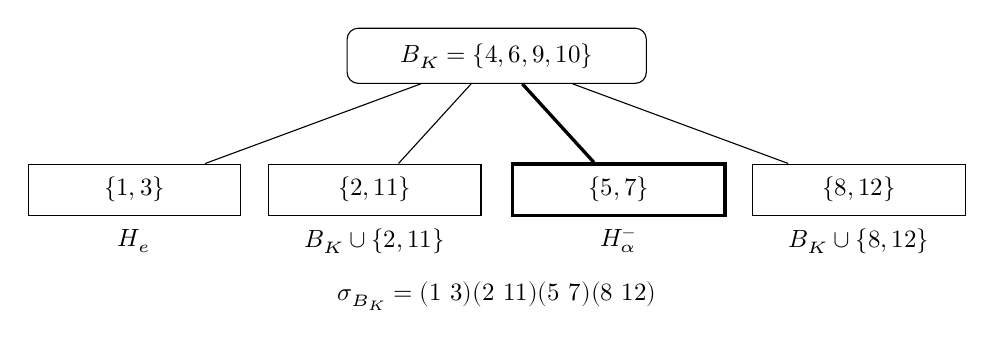
\begin{tikzpicture}[x=1cm,y=1cm, every node/.style={font=\small}]
 \node[draw,rounded corners,minimum width=3.8cm,minimum height=.7cm]
  (b) at (0,0) {$B_K=\{4,6,9,10\}$};
 \node[draw,minimum width=2.7cm,minimum height=.65cm]
  (p1) at (-4.6,-1.7) {$\{1,3\}$};
 \node[draw,minimum width=2.7cm,minimum height=.65cm]
  (p2) at (-1.55,-1.7) {$\{2,11\}$};
 \node[draw,very thick,minimum width=2.7cm,minimum height=.65cm]
  (p3) at (1.55,-1.7) {$\{5,7\}$};
 \node[draw,minimum width=2.7cm,minimum height=.65cm]
  (p4) at (4.6,-1.7) {$\{8,12\}$};
 \draw (b) -- (p1); \draw (b) -- (p2);
 \draw[very thick] (b) -- (p3); \draw (b) -- (p4);
 \node at (-4.6,-2.35) {$H_e$};
 \node at (-1.55,-2.35) {$B_K\cup\{2,11\}$};
 \node at (1.55,-2.35) {$H^-_\alpha$};
 \node at (4.6,-2.35) {$B_K\cup\{8,12\}$};
 \node at (0,-3.05)
  {$\sigma_{B_K}=(1\ 3)(2\ 11)(5\ 7)(8\ 12)$};
\end{tikzpicture}
\caption{The concrete star of the dodecaphasic flag. Each line
indicates the union of the central four-element set with the pair at its endpoint; the
thick line marks the hexad also selected by the signs
preceding the carry of $\alpha$. The four pairs exhaust the eight
outer positions.}
\label{exc:fig-estrella}
\end{figure}

\begin{proposition}[The collection of stars]
\label{exc:m12}
The $\binom{12}4=495$ permutations $\sigma_B$ preserve $\mathcal H$.
The group they generate has order $95040$ and is the Mathieu group
$M_{12}$ in its action on the small Witt design.
\end{proposition}

\begin{proof}
The preservation claim is a finite check on the
$132$ hexads of \eqref{exc:codigo}: for each four-element set the
four petals are constructed and one verifies
$\{\sigma_B(H):H\in\mathcal H\}=\mathcal H$.
Closure under composition of these permutations produces $95040$
elements. In the lexicographic enumeration, it suffices to add successively
six stars not yet contained in the group; the intermediate orders
are $2,6,18,360,7920,95040$, and all $495$ stars belong to the final
group. The procedure and the six generators are made explicit in
the technical provenance note. Finally, one applies the recognition
of the automorphism group of $S(5,6,12)$ as $M_{12}$, whose order is
$12\cdot11\cdot10\cdot9\cdot8=95040$.
\end{proof}

An individual star generates a cyclic group of order two. It does
not by itself generate $M_{12}$, still less the Monster. Nor does the
existence of $495$ generators of a permutation group prove that
each is the transport of a specific TPK loop. That assertion
requires the corresponding loop map; the result established here
is the finite incidence action.

\begin{remark}[Equality of traces does not identify operators]
On $V_{11}$, a star has spectrum $+1$ with multiplicity seven
and $-1$ with multiplicity four. Its normalized trace is $3/11$.
A rank-three projector on the same space also has normalized
trace $3/11$, but spectrum $1^3,0^8$. They are not conjugate: their
minimal polynomials and spectra differ. The intertwiner
\eqref{exc:incidencia} transports defined operators; it does not turn
this scalar coincidence into an equivalence of operators.
\end{remark}

\subsection{The binary residue and the five regions of \texorpdfstring{$\pi$}{pi}}
\label{exc:cinco-regiones}

The next recognition uses the extended binary Golay code
$G_{24}$, with parameters $[24,12,8]_2$. Its weights are
$0,8,12,16,24$, and the weight-eight supports form the design
$S(5,8,24)$. Fix a dodecad $D$, the support of a weight-twelve
word. This datum and the incidence isomorphism to be declared
below belong to the realization chart; they are not used to
generate or select the decimals of $\pi$.

\begin{proposition}[Residue of a dodecad and lifting of hexads]
\label{exc:residuo-binario}
The set
\[
 \mathcal H(D)=
 \{O\cap D: O\text{ is an octad},\ |O\cap D|=6\}
\]
is an $S(5,6,12)$ system on $D$. Each of its hexads has
a unique lift to an octad. For any four-element set $B\subset D$,
the five octads containing it split into four residual
lifts and a unique octad $O_B^\perp$ with $O_B^\perp\cap D=B$.
\end{proposition}

\begin{proof}
A five-element set $A\subset D$ belongs to a unique octad $O$. If
$j=|O\cap D|$, the binary word given by the sum of $O$ and $D$ has weight
$20-2j$. Among the permitted weights, with $0\leq j\leq8$, only
$j=2,4,6$ are possible. Since $A\subset O\cap D$, we have $j\geq5$
and therefore $j=6$. This gives existence and uniqueness of the residual
hexad, as well as uniqueness of its lift by selecting five of its
points. Moreover,
\[
 \lambda_4(S(5,8,24))=\frac{\binom{20}1}{\binom41}=5,
 \qquad
 \lambda_4(S(5,6,12))=4.
\]
The four residual hexads on $B$ give four distinct octads.
The fifth cannot meet $D$ in six points, since it would be another residual
hexad; because it contains $B$, its intersection has size four and
equals $B$.
\end{proof}

A hexad-preserving chart $\ell:[12]\to D$ identifies
$\mathcal H$ with $\mathcal H(D)$. Its existence is the recognition
of the design already constructed as the small Witt design; a concrete
choice of $\ell$ fixes the relabeling. The lift
\[
 \iota_D:\mathcal H\longrightarrow
       \{\text{octads of }G_{24}\},
 \qquad H\longmapsto O\text{ such that }O\cap D=\ell(H),
\]
is injective because intersection with $D$ recovers $\ell(H)$.
The domain of this injectivity is the hexads, not the record $K$.

The relation to the five regions of $\pi$ preserves richer data
than the number five. The emissions and their signatures are:
\begin{center}
\small
\begin{tabular}{@{}crll@{}}
\toprule
Region & Multiplicity & Emission $U_6$ & Signature \\
\midrule
$\perp$ & $432$ & $(501,614,498,169,272,272)$ & $555555$ \\
$++_1$ & $144$ & $(810,923,870,169,272,272)$ & $339555$ \\
$++_2$ & $144$ & $(810,983,810,169,272,272)$ & $393555$ \\
$++_3$ & $144$ & $(870,923,810,169,272,272)$ & $933555$ \\
$--$ & $144$ & $(870,923,810,418,674,521)$ & $933717$ \\
\bottomrule
\end{tabular}
\end{center}
In each three-digit decimal block, the signature uses the modular
difference of the first two digits. The five emissions have the
same visible tritic word $w_\pi=010211$, but not the same
regional genealogy. The three positive regions preserve the tail
$169|272|272$; the negative region changes it to $418|674|521$;
the transverse region has a constant signature and greater multiplicity.

The marked extension of the regional chart sends the transverse region
to $O_{\ell(B_K)}^\perp$, the negative region to $\iota_D(H^-_\alpha)$, and the
three positive regions to the other three lifts of the star. This
realizes the $4+1$ partition of the five octads on $\ell(B_K)$.
The individual correspondence between the three positive names and
the three remaining petals requires a chart order; incidence does not
determine it without that datum. The precise claim is therefore a
marked correspondence of regions, compatible with their roles and with
the flag, not a canonical bijection inferred from the cardinality five.

The identity $432+4\cdot144=1008$ preserves the regional
multiplicities. Also, $1008=36\cdot28$, and an octad has
$\binom82=28$ pairs. These equalities are arithmetic catalog
checks, not substitutes for the map $\iota_D$ or the regional chart.

\subsection{From the ternary code to the Niemeier lattice}
\label{exc:niemeier}

The passage to dimension twenty-four need not first go through the
binary code. It is performed directly from $C_W$ by discriminant
gluing. Two compatible prolongations thus remain distinct:
one preserves the residue $W_{12}\subset W_{24}$; the other constructs the
lattice on which the vertex operator algebra will be realized.

Let $A_2=\mathbb Z a_1\oplus\mathbb Z a_2$ with Gram matrix
\[
 \begin{pmatrix}2&-1\\-1&2\end{pmatrix},
 \qquad \rho=a_1+a_2,\qquad \rho^2=2.
\]
Represent the three classes of $A_2^*/A_2$ by
\[
 \varpi_0=0,\qquad
 \varpi_1=\frac{2a_1+a_2}{3},\qquad
 \varpi_2=\frac{a_1+2a_2}{3}.
\]
The map $j\mapsto\varpi_j+A_2$ additively identifies
$\mathbb F_3$ with this discriminant. For $c\in C_W$, write
$\phi(c)=(\varpi_{c_1},\ldots,\varpi_{c_{12}})$ and define
\begin{equation}
 N(C_W)=\bigcup_{c\in C_W}\bigl(A_2^{12}+\phi(c)\bigr).
 \label{exc:niemeier-def}
\end{equation}

\begin{theorem}[Ternary gluing]
\label{exc:niemeier-teorema}
The object \eqref{exc:niemeier-def} is a positive, even,
unimodular lattice of rank $24$. Its root system is exactly
$A_2^{12}$; it is therefore recognized as the Niemeier lattice with
that root system.
\end{theorem}

\begin{proof}
Linearity of the code makes the union of classes stable under
addition. Self-orthogonality annihilates the discriminant pairing:
the latter is a multiple of $c\cdot d/3$ modulo $\mathbb Z$. Thus the
lattice is integral. The norm of a glue class is
$2\operatorname{wt}(c)/3$ modulo $2\mathbb Z$. The weights in
\eqref{exc:enumerador} are multiples of three, so the lattice is even.

The index of $A_2^{12}$ in $N(C_W)$ is $|C_W|=3^6$. Consequently,
\[
 \det N(C_W)=\frac{3^{12}}{(3^6)^2}=1.
\]
Positivity follows from the orthogonal sum of the twelve $A_2$ metrics.
In a nonzero class of $A_2^*/A_2$, the minimum norm is $2/3$;
every nonzero word has at least six nonzero positions.
Hence a vector in a nontrivial glue class has norm
at least $6\cdot2/3=4$. No norm-two roots occur outside
$A_2^{12}$. Within it, the roots are precisely those of its
twelve components.
\end{proof}

\subsection{Incidence selection of the rootless unimodular neighbor}
\label{exc:leech}

The label $o_*=1$ of the flag is now realized as one of the
twelve $A_2$ components. This operation declares the preceding metric and
the positive radial chamber
\[
 v(a)=\sum_{i=1}^{12}a_i\rho_i,
 \qquad a_i=1+3b_i,\quad b_i\in\mathbb Z_{\geq0}.
\]
The evenness requirement for the index-three neighbor is
$v(a)^2\equiv0\pmod{18}$. Since
\[
 v(a)^2=2\sum_i(1+3b_i)^2,
\]
this congruence is equivalent to $\sum_i b_i\equiv1\pmod3$. The least
norm in the chamber is obtained with a single $b_i=1$ and
all others zero; it is $54$. The marked origin selects
\begin{equation}
 v_\alpha=4\rho_1+\rho_2+\cdots+\rho_{12},
 \qquad v_\alpha^2=54.
 \label{exc:vector}
\end{equation}
The word ``least'' refers to this positive chamber. It does not assert
minimality throughout the residual class: the vector
$(a_1-2a_2,\rho,\ldots,\rho)$ represents the same class modulo three
and has norm $14+11\cdot2=36$. The chamber restriction is part
of the construction data, not an omissible conclusion.

Let $N=N(C_W)$. Define
\begin{equation}
 N_{\alpha,0}=\{x\in N:\langle x,v_\alpha\rangle\equiv0\pmod3\},
 \qquad
 N_\alpha=N_{\alpha,0}+\mathbb Z\frac{v_\alpha}{3}.
 \label{exc:vecino}
\end{equation}

\begin{theorem}[Leech neighbor determined by the marked flag]
\label{exc:teorema-leech}
With the declared metric and chamber, $N_\alpha$ is a positive, even,
unimodular lattice of rank $24$, with no vectors of norm two.
By the corresponding classification theorem, it is isometric to the
Leech lattice $\Lambda_{24}$.
\end{theorem}

\begin{proof}
The character $x\mapsto\langle x,v_\alpha\rangle\bmod3$ is nonzero:
a simple root of a component pairs with $a_i\rho_i$ to give
$a_i\equiv1\pmod3$. Hence $[N:N_{\alpha,0}]=3$ and
$\det N_{\alpha,0}=9$. Moreover,
$v_\alpha/3\in N_{\alpha,0}^*$ and $v_\alpha\in N_{\alpha,0}$.
If $v_\alpha/3$ belonged to $N$, the integrality of $N$ would make
all pairings with $v_\alpha$ divisible by three,
contradicting the nonzero character. The class of $v_\alpha/3$ therefore
has order three. It follows that
\[
 [N_\alpha:N_{\alpha,0}]=3,
 \qquad \det N_\alpha=9/3^2=1.
\]
The extension is integral, and for $x\in N_{\alpha,0}$,
\[
 \left(x+m\frac{v_\alpha}{3}\right)^2
   =x^2+2m\frac{\langle x,v_\alpha\rangle}{3}+6m^2
   \in2\mathbb Z.
\]
Hence it is even.

It remains to exclude roots, the decisive step. The roots of $N$
belong to $A_2^{12}$. Their pairings with $v_\alpha$ are
congruent to $\pm1$ or $\pm2$ modulo three; none belongs to
$N_{\alpha,0}$. For the other two classes of the neighbor, each component
belongs to one of the local classes
\[
 A_2+\varpi_j\pm\rho/3,\qquad j=0,1,2.
\]
Since $4\rho/3\equiv\rho/3\pmod{A_2}$, this description also holds
in the distinguished component. Writing a local vector
as $(u a_1+v a_2)/3$, its norm is
$2(u^2-uv+v^2)/9$. The six preceding classes have nonzero residues
and minimum $2/9$: representatives minimizing the quadratic form
are $(\pm1,0),(0,\pm1),(1,1),(-1,-1)$ in the appropriate residues.
A vector in a new class therefore has norm at least
$12\cdot2/9=8/3>2$. There are no roots in any of the three classes.
The classification of positive even unimodular lattices of
rank twenty-four identifies the unique rootless case with
$\Lambda_{24}$.
\end{proof}

The argument does not recognize Leech from a coincidence of dimension.
It constructs the gluing, proves integrality, evenness, and the determinant, and
eliminates roots through a local bound. Only then does it apply the
classification theorem. The dependence on $\alpha$ is preserved in
the flag selecting $o_*$ and in the vector \eqref{exc:vector};
the scalar value of the constant is not converted into a length of the
lattice.

\subsection{The vertex operator algebra and the Monster}
\label{exc:voa}

Let $\Lambda=N_\alpha$, already recognized as Leech. The next step
uses its integral lattice, not a decimal expansion. The lattice
vertex operator algebra construction is written
\[
 V_\Lambda=M(1)\otimes\mathbb C_\varepsilon[\Lambda].
\]
Here $M(1)$ is the rank-twenty-four Heisenberg oscillator
space; $\mathbb C_\varepsilon[\Lambda]$ is the group algebra
twisted by the cocycle of the central extension of the lattice. The
cocycle and the lift of the isometries are part of the
construction: a bare vector-space sum does not determine the vertex
products.

Negation $\lambda\mapsto-\lambda$ admits the standard lift
$\theta$. With its twisted module and the compatible parity choice,
the Frenkel--Lepowsky--Meurman construction produces
\begin{equation}
 V^\natural_{\rm HMT}
   =V_\Lambda^+\oplus(V_\Lambda^T)^+.
 \label{exc:flm}
\end{equation}
The sign $+$ denotes the even part of the lifted action. The expression
includes the orbifold vertex product; it is not merely a sum
of graded spaces.

\begin{theorem}[Prolongation to the Moonshine module]
\label{exc:moonshine}
The algebra \eqref{exc:flm}, constructed on the neighbor
\eqref{exc:vecino}, is a realization of the Moonshine algebra
$V^\natural$. It has central charge $24$, zero weight-one component,
and automorphism group isomorphic to the Monster $\mathbb M$. Its graded
character is
\begin{equation}
 \operatorname{Tr}_{V^\natural_{\rm HMT}}q^{L_0-1}
   =J(\tau)=j(\tau)-744
   =q^{-1}+196884q+21493760q^2+\cdots,
 \qquad q=e^{2\pi i\tau}.
 \label{exc:j}
\end{equation}
\end{theorem}

\begin{proof}
Theorem \ref{exc:teorema-leech} verifies the lattice hypotheses:
positivity, evenness, unimodularity, rank twenty-four, and absence of
roots. The Frenkel--Lepowsky--Meurman construction and theorem
for the Leech lattice then apply. They identify
the orbifold with $V^\natural$ and establish its character and its
automorphism group. Composing the flag, the neighbor, and the VOA
construction functor gives the realization stated here. The group is not inferred
from the coefficient $196884$.
\end{proof}

The theorem used is a subsequent classical recognition with verified
hypotheses, not a new proof of the FLM construction in this article
\cite{flm}.
Moreover, the notation $q=e^{2\pi i\tau}$ is the conventional Fourier
variable used to recognize the character. It does not introduce $\pi$
or $e$ as inputs into the coinductive generator that has already determined them.

Part of the trace mechanism can be seen before the orbifold.
Only the zero lattice vector is fixed by negation; each
oscillator contributes an alternating sign. Hence
\[
 \operatorname{Tr}_{V_\Lambda}\theta q^{L_0-1}
   =t_2(\tau)
   :=q^{-1}\prod_{n\geq1}(1+q^n)^{-24}.
\]
This trace in the lattice algebra must not be confused with the
character of $V^\natural$ without insertion. Nor does it by
itself identify a Monster conjugacy class: the space, insertion,
and lift must be specified before functions are compared.

\subsection{Graded Moonshine traces and representation of the Monster}
\label{exc:alcance}

For $g\in\operatorname{Aut}(V^\natural_{\rm HMT})$, the trace
with insertion is
\[
 T_g(\tau)=
 \operatorname{Tr}_{V^\natural_{\rm HMT}}gq^{L_0-1}.
\]
The monstrous Moonshine theorem identifies these series as
Hauptmoduln of the corresponding genus-zero groups
\cite[Theorem~1.1]{borcherds}.
The character $J$, the group $\mathbb M$, and the collection $g\mapsto T_g$
are realizations of the algebra already constructed. They do not form a causal
sequence in which one first guesses $J$ and then infers the Monster.

The unit has a precise algebraic location here. The weight-zero
subspace is the vacuum line, \(V^\natural_0=\CC\mathbf1\), and
the coefficient of \(q^{-1}\) in \(J\) is therefore \(1\). In weight one
the dimension is zero, accounting for the absence of the constant term
in \(J=j-744\). A morphism of vertex algebras preserves the vacuum
vector. This property provides the technical meaning of preservation
of the unit at this level; the unit of cylindrical observables
is preserved by the precomposition proved earlier. The relation
between the two levels must follow the construction maps with their units.

In weight two, the equality
\[
 196884=1+196883=196560+324=54(5\cdot729+1).
\]
appears. The first decomposition corresponds to the trivial conformal line and the
irreducible component of dimension $196883$ in the Monster
representation. The other expressions have lattice-theoretic or
arithmetic readings. Their equality does not automatically identify their summands
with TPK regions, words, or routes. Doing so would require
presenting the maps between those spaces and proving that they respect the
relevant actions.

\par
In particular, an isometry $N_\alpha\simeq\Lambda_{24}$ induces
a realization of \eqref{exc:flm}, and a choice of isomorphism
with $V^\natural$ transports its automorphism group. This does not
construct an action of the Monster on the digits of
$\pi$, on the blocks of $K$, or on all TPK histories.
Such an additional assertion would require a representation
$\rho_{\rm TPK}$ and a map $F$ with an explicit square
\[
 F\rho_{\rm TPK}(g)=\rho_{V^\natural}(g)F,
\]
including domain, codomain, and preserved information. The absence
of that step from the present claim does not remove the incidence
intertwiner $U_W$, the flag, or the neighbor already constructed; it only
delimits a different promotion, namely an action on the source state.

The chain established in this section can be summarized, keeping
its transport data visible, as
\begin{align*}
 &\text{APP--TRIT--TPK and arithmetic state with trajectory memory}
   \longrightarrow (w_j,f_j;K,s_0)\\
 &\longrightarrow (C_W,\mathcal H;B_K\subset H^-_\alpha,
                   P_\pi,H_e,H_\varphi,H_{\rm APP})\\
 &\longrightarrow \bigl(N(C_W),o_*,\text{metric and chamber}\bigr)
   \longrightarrow N_\alpha
   \longrightarrow V^\natural_{\rm HMT}.
\end{align*}
At the incidence level, the stars generate $M_{12}$, and the
residual chart realizes the regional $4+1$ structure in $W_{24}$.
At the lattice and VOA level, the construction gives Leech and the
Moonshine module. These are prolongations of the same marked source, with
different objects and maps. Causal continuity does not require
identifying their codomains or erasing the explicit choices
of frame, chamber, and lift.

The result of this section is therefore an assembled derivation:
the finite and lattice proofs make the passage from dodecaphasic
incidence to the hypotheses of the recognition theorems effective.
The conclusion is algebraic: it preserves incidence, lattice structure,
and the resulting module under the declared choices of frame, chamber,
and lift. Mathematical recognition is distinct from the experimental
comparison of constants.

\clearpage% Provenance: RESULTADO_RECUPERADO from chapter 24 of the 2249-page integral
% and FORMA_ELIPTICA_RADIO_MODULAR_ACCION_ORIENTADA.md (D04).
% Expository delta: the diagonal operator domain written out fully and
% integer recovery in the two quotient charts made explicit.
% External label dependency: sec:ellipse. Bibliography: elipse,
% hmtedicionintegral, flm, borcherds. No new macros required.

\section{From the action ellipse to T-duality}
\label{sec:ii-dualidad-t}

The reciprocity of the ellipse provides a shape coordinate for the
exchange between visible value and boundary memory. The antecedent is the
same enriched APP--TRIT--TPK state: APP preserves the sum
and product sheets with their remainders and quotients; TRIT preserves their orientation;
TPK transports sheet, carry, route, and memory. The angular and
action outputs already constructed on the joint discrete structure of the continuum
then determine the ellipse. This section composes its subsequent readers:
elliptic shape, lattice exchange, momentum--winding realization,
and modular evaluation \cite{elipse,hmtedicionintegral}.

The cutoff thus lies after the generation of
\(A,C^*,\hbar\). No prescribed radius or string constant selects
those outputs. Boundary memory is first preserved in the
remainder--quotient pair and then transported through the maps proved
below.

\subsection{The action shape determines the normalized radius}

Return to the chart of section~\ref{sec:ellipse}. Let \(A\ne0\),
\(\hbar>0\), and \(|C^*/A|<1\), with both angles expressed in the same
unit. The semiaxes remain labeled:
\begin{equation}
 \eta_{\rm el}=\operatorname{artanh}(C^*/A),\qquad
 a_S=\sqrt{2\hbar}\,e^{\eta_{\rm el}/2},\qquad
 b_S=\sqrt{2\hbar}\,e^{-\eta_{\rm el}/2}.
 \label{eq:ii-t-elipse}
\end{equation}
The balanced phase coordinates and their semiaxes have units of the square root
of action. The radius below is dimensionless.

\begin{proposition}[Shape radius and labeled reciprocity]
\label{prop:ii-t-radio}
The rectangular chart of the ellipse uniquely determines
\begin{equation}
 R_0=\sqrt{\frac{b_S}{a_S}}
 =e^{-\eta_{\rm el}/2}
 =\left(\frac{A-C^*}{A+C^*}\right)^{1/4}>0,
 \qquad \tau_{\rm el}=iR_0^2.
 \label{eq:ii-t-radio}
\end{equation}
It preserves the signed angular ratio through
\begin{equation}
 \frac{C^*}{A}=\frac{1-R_0^4}{1+R_0^4}.
 \label{eq:ii-t-recuperacion-angular}
\end{equation}
Exchanging the labeled semiaxes transforms
\((\eta_{\rm el},R_0,\tau_{\rm el})\) into
\((-\eta_{\rm el},R_0^{-1},-1/\tau_{\rm el})\), leaving
the scale \(a_Sb_S=2\hbar\) fixed.
\end{proposition}

\begin{proof}
Dividing the semiaxes of~\eqref{eq:ii-t-elipse} gives
\(b_S/a_S=e^{-\eta_{\rm el}}\). The map \(R\mapsto R^2\)
is bijective on \(\mathbb R_{>0}\), so its positive root is
unique. For \(x=C^*/A\in(-1,1)\),
\(2\operatorname{artanh}x=\log((1+x)/(1-x))\); hence
\(R_0^4=(1-x)/(1+x)\). Solving for \(x\) proves
\eqref{eq:ii-t-recuperacion-angular}. Exchanging \(a_S,b_S\)
inverts their ratio and changes the sign of \(\eta_{\rm el}\). Finally,
\(-1/(iR_0^2)=iR_0^{-2}\), while the product of the semiaxes
remains \(2\hbar\).
\end{proof}

The angular ratio is recovered; the two absolute angles and their generating
history continue to reside in the enriched state. The point \(R_0=1\)
corresponds to the circular shape \(C^*/A=0\), not to an identification of
all orientations or all histories.

\subsection{Lattice exchange and equivalence of operators}

\begin{definition}[Stable domain of the dual reading]
\label{def:ii-t-reticular}
On \(\mathscr D_0=\mathbb Z^2\times\mathbb R_{>0}\), define
\begin{equation}
 E_{R_0}(m,w)=\frac{m^2}{R_0^2}+w^2R_0^2,\qquad
 \mathsf T_0(m,w,R_0)=(w,m,R_0^{-1}).
 \label{eq:ii-t-energia}
\end{equation}
The first coordinate prolongs the visible reading, and the second the quotient
reading. The full integer domain permits their exchange without requiring
the quotient to belong to a section of nine representatives.
\end{definition}

For the radius of~\eqref{eq:ii-t-radio}, the matrix of this form is
\begin{equation}
 D(\eta_{\rm el})=
 \begin{pmatrix}e^{\eta_{\rm el}}&0\\0&e^{-\eta_{\rm el}}\end{pmatrix}
 =\frac{1}{2\hbar}
 \begin{pmatrix}a_S^2&0\\0&b_S^2\end{pmatrix}.
 \label{eq:ii-t-matriz}
\end{equation}
Indeed, \(R_0^{-2}=e^{\eta_{\rm el}}\) and
\(R_0^2=e^{-\eta_{\rm el}}\). The ellipse equation
\(Q^2/a_S^2+P^2/b_S^2=1\), multiplied by \(2\hbar\), uses
the inverse matrix \(D(-\eta_{\rm el})\). This distinguishes
the squared-semiaxis matrix from the matrix of the elliptic equation.

\begin{theorem}[Lattice duality and unitary conjugation]
\label{thm:ii-t-unitaria}
The transformation \(\mathsf T_0\) is involutive and satisfies
\begin{equation}
 E_{R_0^{-1}}(w,m)=E_{R_0}(m,w).
 \label{eq:ii-t-invariancia}
\end{equation}
On \(\mathcal H_{\rm lat}=\ell^2(\mathbb Z^2)\), let \(H(R_0)\)
be the diagonal operator with values \(E_{R_0}(m,w)\), with domain
\[
 \mathcal D(H(R_0))=
 \left\{c\in\ell^2(\mathbb Z^2):
 \sum_{m,w\in\mathbb Z}E_{R_0}(m,w)^2|c_{m,w}|^2<\infty\right\}.
\]
Then \(H(R_0)\) is self-adjoint and nonnegative. The exchange
\(U_T|m,w\rangle=|w,m\rangle\) is a unitary involution that
transports the domains and satisfies
\begin{equation}
 U_T H(R_0)U_T^{-1}=H(R_0^{-1}).
 \label{eq:ii-t-conjugacion}
\end{equation}
\end{theorem}

\begin{proof}
Exchanging the integers twice and inverting the radius twice returns
the initial point. Moreover,
\[
 E_{R_0^{-1}}(w,m)=w^2R_0^2+m^2R_0^{-2}=E_{R_0}(m,w).
\]
The diagonal domain contains the finitely supported sequences and is dense.
Multiplication by a real sequence is symmetric on that domain.
If \(c\) belongs to the adjoint domain, evaluation against each
basis vector forces the adjoint to have coordinates
\(E_{R_0}(m,w)c_{m,w}\). Their membership in \(\ell^2\) is equivalent
exactly to the condition defining \(\mathcal D(H(R_0))\).
Hence the operator and its adjoint agree. Its nonnegative diagonal values
prove positivity.

The exchange bijectively permutes the orthonormal basis, so it is
unitary and its own inverse. For every sequence \(c\),
\[
 \sum_{m,w}E_{R_0^{-1}}(m,w)^2|(U_Tc)_{m,w}|^2
 =\sum_{m,w}E_{R_0}(m,w)^2|c_{m,w}|^2.
\]
This equality proves exact transport of domains. Finally,
\((U_TH(R_0)U_T^{-1}c)_{m,w}=E_{R_0}(w,m)c_{m,w}
=E_{R_0^{-1}}(m,w)c_{m,w}\); this proves
\eqref{eq:ii-t-conjugacion} on the entire domain, not only on the basis.
\end{proof}

Orientation adds information that energy does not distinguish. In the phase
plane, the exchange \(S_2(Q,P)=(P,Q)\) and rotation
\(J_2(Q,P)=(-P,Q)\) transport the same quadratic form, but
\(S_2^*(dQ\wedge dP)=-dQ\wedge dP\) and
\(J_2^*(dQ\wedge dP)=dQ\wedge dP\). With
\(\lambda=P\,dQ\), one obtains directly
\[
 S_2^*\lambda=d(PQ)-\lambda,\qquad
 J_2^*\lambda=\lambda-d(PQ).
\]
Integration over a closed curve gives opposite actions under \(S_2\)
and equal actions under \(J_2\). Thus the index exchange in
\eqref{eq:ii-t-energia} and the symplectic transport of a trajectory
are different maps, even when they yield the same energy.

\subsection{Nonadic sections and carry transport}

For \(n\in\mathbb Z\), the positive section writes
\[
 r_9^+(n)=1+((n-1)\bmod9),\qquad
 Q_9^+(n)=\frac{n-r_9^+(n)}9,\qquad n=r_9^+(n)+9Q_9^+(n).
\]
The remainder of \(n-1\) is taken in \(\{0,\ldots,8\}\). The change to
the remainder section \(0,\ldots,8\) is
\begin{equation}
 C(r,Q)=\bigl(r-9\varepsilon,Q+\varepsilon\bigr),\qquad
 \varepsilon=\begin{cases}1,&r=9,\\0,&r\ne9.\end{cases}
 \label{eq:ii-t-acarreo}
\end{equation}
Thus \(r+9Q\) remains fixed. For \(n=9\), the two coordinates
are \((9,0)\) and \((0,1)\): their uncorrected energies are
\(81/R_0^2\) and \(R_0^2\). Equality of the integer does not imply
equality of those energy insertions. The following covariant form
resolves the change of section without removing carry.

\begin{definition}[Two quotient charts of the nonadic reading]
\label{def:ii-t-cociente}
Let \(L_9=\mathbb Z(9,-1)\), \(S(m,w)=(w,m)\), and
\(L_9^\vee=SL_9=\mathbb Z(-1,9)\). For
\(L\in\{L_9,L_9^\vee\}\), define
\[
 \mathcal E_{R_0}^{L}([x]_L)
 =\min_{\ell\in L}E_{R_0}(x+\ell).
\]
Transport between charts is
\[
 \mathsf T_{\rm cov}:
 (\mathbb Z^2/L_9)\times\mathbb R_{>0}
 \longrightarrow
 (\mathbb Z^2/L_9^\vee)\times\mathbb R_{>0},\qquad
 ([x]_{L_9},R_0)\longmapsto([Sx]_{L_9^\vee},R_0^{-1}).
\]
\end{definition}

\begin{theorem}[Covariance with crossing memory]
\label{thm:ii-t-cociente}
The preceding energies and transport are well defined. The change
of section~\eqref{eq:ii-t-acarreo} preserves the class in
\(\mathbb Z^2/L_9\), and
\begin{equation}
 \mathcal E_{R_0^{-1}}^{L_9^\vee}([Sx]_{L_9^\vee})
 =\mathcal E_{R_0}^{L_9}([x]_{L_9}).
 \label{eq:ii-t-covariancia}
\end{equation}
The return exchange recovers the initial class and radius. The
integer coordinate maps \(N([x])=x_1+9x_2\) and
\(N^\vee([y])=9y_1+y_2\) are isomorphisms with \(\mathbb Z\)
and satisfy \(N^\vee([Sx])=N([x])\).
\end{theorem}

\begin{proof}
Replacing \(x\) with \(x+\ell_0\), where \(\ell_0\in L\),
permutes the candidates for the minimum. This minimum exists: for \(L=L_9\),
\[
 E_{R_0}(x+k(9,-1))
 =\left(\frac{81}{R_0^2}+R_0^2\right)k^2
  +2\left(\frac{9x_1}{R_0^2}-x_2R_0^2\right)k+E_{R_0}(x),
\]
which tends to infinity with \(|k|\); for \(L_9^\vee\), the
leading coefficient is \(R_0^{-2}+81R_0^2>0\). The change
\(C(x)-x=-\varepsilon(9,-1)\) belongs to \(L_9\).
If \(x'-x\in L_9\), then \(Sx'-Sx\in L_9^\vee\),
proving that transport is well defined. By
\eqref{eq:ii-t-invariancia},
\[
 \min_{\ell\in L_9}E_{R_0^{-1}}(Sx+S\ell)
 =\min_{\ell\in L_9}E_{R_0}(x+\ell).
\]
This proves~\eqref{eq:ii-t-covariancia}; \(S^2=I\) proves
the return between the two charts.

Finally, the homomorphism \(x\mapsto x_1+9x_2\) is
surjective and its kernel is exactly \(L_9\), since
\(x_1=-9x_2\). Similarly, the kernel of
\(y\mapsto9y_1+y_2\) is \(L_9^\vee\). Their induced maps
on the quotients are therefore isomorphisms. Substituting
\(y=Sx\) proves the final identity.
\end{proof}

The recovered integer determines its remainders and quotients once the
section is fixed. The energy-minimizing representative need not be that
canonical representative. The quotient is a covariant representation of the
nonadic reading; the source state also preserves sheet, route, orientation,
boundary, memory, and survival. Nor is \(L_9^\vee\) replaced
by \(L_9\): the exchange is between two transported charts.

\subsection{Momentum, winding, and realization scale}

The circular realization introduces an explicit dimensional chart.
Denote its radius by \(R>0\) and let \(\alpha'>0\) be a parameter
with dimension length squared. This symbol differs from the dimensionless
output \(\alpha_{\rm HMT}\). Fixing the chart does not alter the
angular generator or the shape radius. The normalization and its inverse are
\[
 \mathcal N_{\alpha'}(m,w,R)
 =\left(m,w,\frac{R}{\sqrt{\alpha'}}\right),\qquad
 R=\sqrt{\alpha'}\,R_0.
\]
The indices are now read as momentum number and winding
number; the zero-mode components, expressed in units of
inverse length, are
\begin{equation}
 p_L=\frac mR+\frac{wR}{\alpha'},\qquad
 p_R=\frac mR-\frac{wR}{\alpha'},\qquad
 E_{\rm str}=\frac{p_L^2+p_R^2}{2}
 =\frac{m^2}{R^2}+\frac{w^2R^2}{\alpha'^2}.
 \label{eq:ii-t-quirales}
\end{equation}

\begin{theorem}[Dimensional conjugation of T-duality]
\label{thm:ii-t-cuerda}
The transformation
\[
 \mathsf T_{\alpha'}(m,w,R)=\left(w,m,\frac{\alpha'}R\right)
\]
is an involution and satisfies
\begin{equation}
 \mathcal N_{\alpha'}\mathsf T_{\alpha'}
 =\mathsf T_0\mathcal N_{\alpha'},\qquad
 E_{\rm str}=\alpha'^{-1}E_0\circ\mathcal N_{\alpha'},
 \label{eq:ii-t-normalizacion}
\end{equation}
where \(E_0(m,w,R_0)=E_{R_0}(m,w)\). It preserves \(E_{\rm str}\),
fixes \(p_L\), and reverses the sign of \(p_R\). For fixed
oscillator data \(N_L,N_R\) and intercepts \(a_L,a_R\),
it also preserves the condition
\begin{equation}
 \frac{\alpha'}4(p_L^2-p_R^2)+N_L-N_R-a_L+a_R=0,
 \quad\text{that is}\quad
 N_L-N_R=a_L-a_R-mw.
 \label{eq:ii-t-nivel}
\end{equation}
\end{theorem}

\begin{proof}
Two applications exchange the indices twice and send
\(R\) to \(\alpha'/(\alpha'/R)=R\). Also,
\[
 \mathcal N_{\alpha'}\mathsf T_{\alpha'}(m,w,R)
 =\left(w,m,\frac{\sqrt{\alpha'}}R\right)
 =\mathsf T_0\mathcal N_{\alpha'}(m,w,R).
\]
Substitution into the normalized form gives
\[
 E_0\left(m,w,\frac R{\sqrt{\alpha'}}\right)
 =\frac{\alpha'm^2}{R^2}+\frac{w^2R^2}{\alpha'}
 =\alpha'E_{\rm str}(m,w,R).
\]
For \(R'=\alpha'/R\), the transformed modes are
\[
 p'_L=\frac{wR}{\alpha'}+\frac mR=p_L,\qquad
 p'_R=\frac{wR}{\alpha'}-\frac mR=-p_R.
\]
Thus both their sum and difference of squares are preserved.
Direct expansion gives \(p_L^2-p_R^2=4mw/\alpha'\), transforming
the first equation of~\eqref{eq:ii-t-nivel} into the second.
The exchange preserves \(mw\); with the other data fixed, it preserves
the full condition.
\end{proof}

With these orientations, the abbreviated formula \(N_L-N_R=nw\) requires
\(a_L=a_R\) and \(n=-m\). Retaining the sign in
\eqref{eq:ii-t-nivel} preserves the dictionary between the two readings.
The proved result covers conjugation of radii, zero modes,
energy, and the declared level compatibility. The dimensional interpretation
identifies coordinates through its chart; it does not turn
\(R_0\) alone into a length or infer a complete field theory
from an equality of energies.

\subsection{Modular evaluation and the Moonshine character}

The exceptional construction already developed preserves the incidence of the same
antecedent up to \(V^\natural\). Its graded character has the expression
\(J(\tau)=j(\tau)-744\), with the modular invariance used in
Moonshine \cite{flm,borcherds}. This \(J\) is a function on the
upper half-plane \(\mathbb H\); it is not the rotation \(J_2\), the
exchange \(S\), or the nonadic holonomy \(\Gamma_9\).

\begin{proposition}[Modular semiconjugacy of the radius]
\label{prop:ii-t-modular}
Let \(\iota:\mathbb R_{>0}\to\mathbb H\),
\(\iota(R_0)=iR_0^2\), and
\(S_{\rm mod}(\tau)=-1/\tau\). Then
\begin{equation}
 S_{\rm mod}\circ\iota(R_0)=\iota(R_0^{-1}),\qquad
 J(iR_0^2)=J(iR_0^{-2}).
 \label{eq:ii-t-modular}
\end{equation}
In particular, the two labeled shapes of the ellipse have the same
value under \(J\).
\end{proposition}

\begin{proof}
The first identity is
\(-1/(iR_0^2)=iR_0^{-2}\). The matrix
\(\left(\begin{smallmatrix}0&-1\\1&0\end{smallmatrix}\right)\)
belongs to \(\mathrm{SL}_2(\mathbb Z)\) and acts on
\(\mathbb H\) as \(S_{\rm mod}\). The modular invariance of
\(J\), established in its exceptional construction, gives
\(J(S_{\rm mod}\tau)=J(\tau)\). Applying it to
\(\tau=\iota(R_0)\) yields the second identity.
Proposition~\ref{prop:ii-t-radio} identifies these two arguments
with the moduli of the ellipses of opposite shapes.
\end{proof}

The composition thus preserves an explicit chain:
\[
 (A,C^*,\hbar)\longmapsto(a_S,b_S)
 \longmapsto R_0\longmapsto iR_0^2\longmapsto J(iR_0^2).
\]
Shape inversion is transported to radius inversion and to
\(S_{\rm mod}\); oriented action and change of section retain
their own maps. The function \(J\) assigns a value to a modular class, while
the marking of the axes distinguishes its two presentations and the TPK state
preserves its genealogy. This is the proved relation between the action
ellipse, T-duality, and Moonshine: a composition with domains and
transport identities, whose modular value replaces neither the lattice
operator nor the construction of \(V^\natural\).

\clearpage% BEGIN THERMAL_R03_SYNC_13
\section{Conclusions}
\label{sec:ii-conclusiones}

The construction obtains the Planck action sections and their return
ratio, evaluates the Barbero--Immirzi parameter from oriented incidence,
and produces the CKM angles with their phase and unitary amplitudes.
It also determines the Boltzmann transducer for a positive thermal
section and the common gravitational coefficient of realization R1--R8,
whose circular specialization retains radius coincidence.
Inscription determines \(r_N=5759/23040\); longitudinal composition
gives \(L=r_N\alpha_{\HMT}^{16}L_*\); the radial metric and action
fix \(G_{\rm ret}=c_{\rm int}^3L^2/\hbar_{\rm ret}\) under the
explicit reduced-radius identification. The resulting identities connect
the constants to their functions: energy per frequency, elementary
area resolution, mixing information, thermal conversion, and geometric
invariance.

The central relation is preservation of the geometric scale.
The product \(G_a\hbar_a\) preserves the area scale while action
and gravitation transform reciprocally; incidence weighted by
\(\gamma_{\HMT}\) determines the resolution of that area; and
\(k_B\Theta_{{\rm clk},a}\log3=h_a/T_{108}\) relates the same action
to the energy of a tritic decision. Joint observation of area and
the modular Hamiltonian, with \(\Delta_{\rm mod}\ne0\) and
known normalization, recovers the sector occupations that a single
aggregate reading does not distinguish. Direct inversion of
\((N,D)\) remains valid without that condition. Each identity retains the
conditions of its dimensional, geometric, or spectral realization.

\subsection{Planck constants, Barbero--Immirzi, and CKM mixing}

The action scale contains two distinct determinations. The
local quotient of the record has sixteen sheets; its multiplicative norm
and autoscaling fix \(\operatorname{ord}_{10}(\varphi\alpha^{16})=-34\). The regional characters fix the oriented sections
and return quotient. Conversion between angular action and action
per turn maintains the identity \(h=2\pi\hbar\). The angular chart
transports representatives in degrees to radians while preserving both
channel arguments and functional coefficients.
This precision allows the dependence of action to be followed without a
retrospective inversion of its coordinates.

The hexadic--octadic transition supplies the specific content of the
Barbero--Immirzi functional. The incidence spaces fix the
cardinalities; the oriented turn fixes the multiplicities; evaluation
of the channels determines the scalar. Its subsequent use in the
area operator and gravitational action makes visible the meaning
of the structure producing the value. The parameter thus serves a
demonstrative function in the relation between incidence, orientation, and
geometry.

The CKM construction determines mixing through an explicit reader. The
rational reader transports the preceding angular coordinates to three
mixing angles and fixes their phase; its inverse reconstructs the initial
coordinates. Unitary factorization makes the amplitudes explicit, and the
Jarlskog invariant preserves CP-violation information under
admissible phase changes. Its quantitative comparison uses
the declared angular convention and physical reference. The leptonic
construction is presented in its own spectral frames, preserving the
distinction between the two species transports.

The numerical mixing results are
\begin{align*}
 (\theta_{12},\theta_{23},\theta_{13})
   &=(13.003313589509,\ 2.398056157332,\ 0.213977382244)^\circ,\\
 \delta_{\rm CP}&=65.676173123554^\circ,\qquad
 J_{\rm CKM}=3.1189723326632974\times10^{-5}.
\end{align*}
Table~\ref{tab:ii-ckm-comparacion} compares their sines, phase and
invariant with PDG 2025 in the same parametrization: all five normalized
marginal deviations satisfy $|z|<0.029$. The result connects the
generated coordinates with unitary amplitudes and with a phase measure
that remains invariant under reparametrization.

The angular realization in Witt incidence establishes an explicit,
polar-normalized isometric transport with inverse on its image.
The metric equality in Corollary~\ref{cor:ii-witt-composed-reader}
specifies its function: composition with the angular reader preserves the
induced metric, distinguishes different angular coordinates, and permits
reconstruction of the three coordinates feeding the sector rules.
Comparison between the record and incidence is thus made through
a faithful map. The determinant representation preserves
orientation; gauge changes transform the data jointly,
according to \ref{prop:ii-witt-gauge-covariance}; the complex realization preserves
phase and the order of the unitary mixing factors. The selection
of sector operations, their evaluation, and transport of their
result remain distinct, without identifying subsequent isometric transport with selection of
the sector rules it evaluates.

\Needspace{11\baselineskip}
\subsection{The Boltzmann constant and energy per tritic decision}

Action and period yield
\(\epsilon_a=h_a/T_{108}=\hbar_a/t_P\); the information of the
uniform ternary distribution fixes the energy per nat \(\epsilon_a/\log3\).
For a fixed positive thermal section \(\Theta_{{\rm clk},a}\),
there is a unique positive linear transducer
\(k_B:\mathcal L_\Theta\to\mathcal L_E\) mapping it to that
energy. Its expression in positive bases retains the transformation
law \(b'=(s_\Theta/s_E)b\). This determines both the dimensional
function of Boltzmann and the conditions that individualize its
coordinate: the thermal section, the bases, and, when internal
selection is claimed, the reader that fixes them.

The same transducer acts on both orientations when the cycle
temperatures have the ratio of the action sections,
as in \eqref{eq:ii-kb-aut-orientaciones}. It assigns the corresponding
entropy quantity to information through \(S=k_Bs\), without identifying a
distribution of continuations with a quantum bipartition or a
reversible update with physical erasure. Energy, information, and
entropy thus retain their domains when related to area and to the
gravitational cell.

The capacity construction in \ref{sec:ii-ter27-antecedentes} retains the
calendar with its vacancies, the two carrier gradings, and the positive
energy realization of memory. The decimal spectrum, capacity origin,
and multiplicities determine intensity \(b_*=1.380649\times10^{-23}\)
under the stated degree assignment. Currents fix the offset in their
connected realization; centered transport preserves the reader and its
reference.

Theorem~\ref{thm:ii-ter27-transducer} adds a precise thermometric
consequence. Fixed reference and trial state produce an entropy increment
\(b_*s\); its joint reading with conditioned energy determines
\(\Theta_P=1/(b_*\beta)\) and a unique positive transducer of coefficient
\(b_*\). Corollary~\ref{cor:ii-ter27-variational} also proves the unique
free-energy minimum. The fixed reference and pair of functionals are
the conditions of that realization. On the graded carrier, the
chronological capacity Hamiltonian gives exactly
\(\rho=q^N/Z_N(q)\); its relation to area and horizon preserves
the different scales and finite relative-entropy identity.

Section~\ref{sec:ii-aditiva-instrumento} supplies the additive
characterization of this weight and the conservative realization of its
marks. Disjoint alternatives, their received measure and the reference
unit fix the contribution $b_*s$; conditioning recovers the mean energy
of the same trial. The instrument preserves the spectral complement,
system energy and tritic transport with quotient and carry. A shared reference
retains a single factor $b_*$ when systems are composed and preserves
their correlations. These proofs specify the operations of the thermal
realization as well as evaluating its coefficient.

\subsection{Gravitation and preservation of the area scale}

The gravitational construction also preserves tensorial information
not exhausted by the scalar coupling section. The incidence descent
of \ref{sec:ii-pentadica}, under its explicit conditions, produces the
five-component carrier. The intertwiner \(\Gamma_5\) realizes that
carrier as symmetric trace-free tensors; its basis distinguishes the weights
\(\pm2,\pm1,0\). Transverse reduction preserves two of them through
a rank-two projector. This sequence simultaneously transmits the
common coupling \(G_a\), the orientation of its five components, and
the reduced observation, according to
\eqref{ii:pent:eq:gravity-12-5-5-2}. The physical interpretation preserves the
dynamics and constraints specified in that development.

Inscription, the complete archive, and longitudinal and metric
compositions first determine the radial reader. Energy and radius act
on the same positive character; cancellation proves that the coupling
coefficient is common to every mode in the declared domain. Rules R4
and R5 remain incorporated compositions, and R8 retains the physical
identification of the reduced radius. The clock
\(t_0=\pi_{\HMT}L/(54c_{\rm int})\) subsequently expresses the
same length in the circular calendar.

Unitary transport preserves the coefficient and the records. Joint
elimination of boundary and memory preserves radial--energy
proportionality, the radial product, and the recoverable residual;
in the complete resolvent the spectral parameter is transported as
well, according to \eqref{g26:eq:resolvente-proporcional-en}.
This conservation includes static and dynamic memory within their
domains. Reciprocity of the action sections preserves the
product of gravitation and action and, with it, the area scale. The
thermal realization links the energy of the elementary duration to
tritic information. In the specified horizon cell, energy,
temperature, entropy, and half-action satisfy the proved
identities. The article thus places the relation between information and
gravity within an explicit mathematical composition.

\subsection{Boundary information and entanglement entropy}

The joint reading of area and sector information provides a
concrete expression of boundary genealogy. Area aggregates
occupations, while the weighted observable preserves their distribution
between the two sectors. Their recovery is proved by
inverting the incidence map. Entanglement entropy adds
the reduced state and bipartition that give it meaning. Transporting
these data allows spectral preservation,
orientation preservation, and preservation of the information accessible
in a reduction to be distinguished.

The sector formulation also obtains the mean area and mean
modular information from the finite partition function. Their
derivatives are expressed through occupation variances and covariances.
Unitary inversion of the occupations preserves entropy and
transforms area into its complement. This specifies a central
phenomenon of the genealogical reading: a conserved quantity can
coexist with a structural transformation detected by another
observable. The Boltzmann transducer preserves its dimensional function
in this relation between information, energy, and entropy.

Transport of the collective modes makes explicit how hexadic--octadic
incidence reaches the area labels. At a fixed reference state,
the modular first law relates variations of
entropy and weighted occupation. For finite changes, the identity
includes the relative entropy between states; retaining that term
specifies the informational content distinguishing an infinitesimal
variation from a finite transformation. Joint recovery
of the occupations through area and incidence places this relation
directly on the two boundary observables.

\subsection{Reciprocity and exceptional continuation}

The action ellipse and T-duality prolong the argument through
transport invariants. Exchanging semiaxes preserves the
determinant of the form; symplectic orientation distinguishes
realizations with the same energy; momentum--winding exchange
preserves the spectral operator under the corresponding domain
identification. The exceptional realization maintains incidence
up to Moonshine and allows modular reciprocity to be formulated in its
own space.

The covariance realization in
section~\ref{sec:ii-area-covarianza} specifies the operator content of
this reciprocity. In the two-standard-deviation normalization,
the area \(h\) fixes
\(\det V_\eta=\hbar^2/4\), while angular anisotropy determines
\(\Delta P/\Delta Q=e^{-\eta}\). The constructed Gaussian state and its
canonical operators realize exactly these two relations; the
symplectic rotation exchanges their dispersions while preserving the
commutator. The action determinant,
ellipse geometry, and uncertainty saturation are thereby related in an
explicit representation. The distinction between contour energy,
\(\hbar\omega\), and mean state energy,
\(\hbar\omega/2\), preserves the normalization of both readings.

The extension to M-theory requires a specification of compactification,
world sheets, and the corresponding physical representations.
The particle--antiparticle relation through orientation, advance, and
delay constitutes a proposed extension, distinct from the covariance
and reciprocity identities proved here.

Section~\ref{delta22:ii:transporte} proves exact conservation of
quadratic action under transport between ellipses, derives its
Hamiltonian connection term, and establishes the positivity condition
of the generator. The conformally symplectic version preserves
normalized action and specifies the transported form.

\subsection{Evaluation of the record and preservation of observation}

The incidence evaluation in
\eqref{eq:registro-composicion-incidencial} makes explicit the operation
converting a ledger of visits and oriented traces into twenty-five
coordinates. Each triple of counts is represented through its decimal
residues, while its quotients and provenance remain in the ledger.
Proposition~\ref{prop:registro-36-residuos} determines when two
collections of counts have the same image. Its content makes it possible
to specify what information the resulting value uses and what additional
information is preserved by the history that produced it. The incidence collection
and traces feeding the evaluator retain their construction
conditions; the subsequent invertibility of the record has a
complementary function: exact recovery of that representation.

Preservation of observation acquires a dynamic formulation in
\ref{subsec:ii-memoria-resolvente}. The finite identity retains the terminal
state of the history; its prolongation controls the contribution of
subsequent increments through a tail bound. When an
auxiliary sector is eliminated, identities
\eqref{mem:schur-fuente}--\eqref{mem:schur-lector} also transport
the source and the reading map. The content of a trajectory
can thus be expressed in fewer components while preserving the effects of
its excursions and returns. The transitivity of
\eqref{mem:schur-transitivo} ensures coherence of this operation
when elimination proceeds in several stages. This is a
precise consequence of treating memory as an operative part of the state.

% BEGIN THERMAL_R03_SYNC_13B
% Consolidated formalization of results already presented in the body.
\subsection{Structural definitions and quantitative results}
\label{sec:ii-conclusiones-cuantitativas}

Definition through structure preserves the object prior to the scalar
reading. For the action constants, that object is an oriented section
with a multiplicative norm over the local quotient and a regional character. For Barbero--Immirzi,
it is the evaluation of an oriented incidence. For mixing, it is a transport
between coordinates and amplitudes. For Boltzmann, it is a map between
lines of quantities. For gravitation, it is a reciprocal action section
whose magnitude follows from the inscribed length and radial reading
specified in R1--R8. These definitions
determine different operations within the same genealogy.

For each quantity, the following table fixes the object that defines it,
the operation that determines its reading, and the physical role developed
in the body. The reconstruction and transport proofs establish
how that information is preserved when the result is reused. In
particular, \ref{prop:registro-36-residuos} characterizes the representation
of the record, \ref{mem:prop-schur} preserves observation under reduction,
and \ref{cor:ii-witt-composed-reader} preserves the angular coordinates
in the incidence realization. These three operations have their own domains
and distinct demonstrative roles within the same sequence.

\begingroup
\setlength{\LTpre}{0pt}
\setlength{\LTpost}{2pt}
\begin{longtable}{@{}p{.13\linewidth}p{.415\linewidth}p{.395\linewidth}@{}}
\caption{Structural object, produced reading, and physical meaning of
the article's results.}\label{tab:ii-conclusiones-estructura}\\
\toprule
Quantity & Structural definition and result & Physical reading and internal development\\
\midrule
\endfirsthead
\toprule
Quantity & Structural definition and result & Physical reading and internal development\\
\midrule
\endhead
\bottomrule
\endfoot
Planck & Section of the action line:
$\hbar_{\rm pre}=H_5\,10^{-34}\mathcal U_S$,
$\hbar_{\rm ret}=\eta_{\rm ret}\,10^{-34}\mathcal U_S$.
The local quotient has sixteen sheets, and
$\operatorname{ord}_{10}(\varphi\alpha^{16})=-34$.
& The section relates frequency and energy; the complete turn determines
$h_a=2\pi\hbar_a$. Development in \ref{sec:action}; coordinates and comparison
in \ref{tab:ii-planck-comparacion}.\\[5pt]
Barbero--Immirzi & Oriented evaluation of the channels and incidence:
$\gamma_{\HMT}=\pi AC^*/180+12\Delta S_{90}-\Delta S_{120}$.
The printed evaluation is $0.2740076726944592747\ldots$.
& The coefficient enters elementary area resolution and
the Cartan--Holst realization. The definitions in
\ref{sec:barbero} and \ref{sec:area} preserve these two uses;
\eqref{eq:holst} specifies the second.\\[5pt]
CKM mixing & Image of the angular vector under the three sectorial
maps; phase $\delta_{\deg}=9A_{\deg}$.
The angles and amplitudes are evaluated after the reader is constructed.
& The Jarlskog quartet expresses phase information invariant
under diagonal basis changes. The rules, their evaluation, and the
unitary realization are developed in
\ref{sec:ii-propagacion-angular}.\\[5pt]
Boltzmann & Positive transduction
$k_B:\mathcal L_\Theta\to\mathcal L_E$ with
$k_B\Theta_{{\rm clk},a}\log3=h_a/T_{108}$.
The state and measure of the continuations determine the information
content on which it acts.
& $S=k_Bs$ dimensionally realizes the entropy of the reduced state.
Energy and temperature bases and their transformations are preserved
in \ref{sec:ii-boltzmann}; the additive characterization and instrument
are proved in \ref{sec:ii-aditiva-instrumento}; the comparison is in
\ref{tab:ii-kb-g-cartas}.\\[5pt]
Marked thermal realization & Fixed reference $\eta$, with multiplicities
$(d_0,d_1,d_2)=(1,380,649)$ at degrees $23,26,29$ and trace
$b_*=1.380649\times10^{-23}$.
The readings $\mathcal S_P=b_*s$ and $\mathcal E_P=\operatorname{Tr}(\rho H)$
determine $d\mathcal S_P/d\mathcal E_P=b_*\beta$ and
$\Theta_P=(b_*\beta)^{-1}$.
& With fixed reference, transported positive bases and a nonscalar
Hamiltonian, \ref{thm:ii-ter27-transducer} determines the transducer.
Corollary~\ref{cor:ii-ter27-variational} proves the unique minimum.
Composition preserves $q^N/Z_N(q)$, the energy origin and the
clock--horizon transports of \eqref{eq:ii-ter27-intertwiner}.\\[5pt]
Gravitation & Reciprocal section
$G_a=c_{\rm int}^{3}L^2/\hbar_a$,
with $L=(5759/23040)\alpha_{\HMT}^{16}L_*$.
The clock $t_0=\pi_{\HMT}L/(54c_{\rm int})$ preserves the circular
expression $G_a=\vartheta_{108}^{\circ}c_{\rm int}^{5}t_0^2/\hbar_a$,
with $\vartheta_{108}^{\circ}=(54/\pi_{\HMT})^2$.
& The product $G_a\hbar_a$ preserves areal normalization.
The longitudinal and radial construction, its rules, and uniqueness
of the coefficient are proved in \ref{g26:sec:rigidez-radial-en};
the circular realization is retained in \ref{sec:gravity} and thermal confluence in
\ref{sec:confluencia}.\\
\end{longtable}
\endgroup

Quantitative comparison preserves the particular meaning of each
reference. For Planck, Table~\ref{tab:ii-planck-comparacion} compares
dimensional coordinates with an SI defining constant; the relative
residuals of the pre-return and post-return orientations are,
respectively, approximately $-1.82\times10^{-15}$ and
$-6.93\times10^{-10}$. For Barbero--Immirzi,
Table~\ref{tab:ii-barbero-comparacion} compares two constructions:
the internal evaluation and the root of the Ghosh--Mitra equation, whose
approximate value is $0.2740668582328300$. The relative difference is
approximately $-2.16\times10^{-4}$; the object compared is a
theoretical coefficient.

For CKM, Table~\ref{tab:ii-ckm-comparacion} brings together the sines of the
three mixing angles, the phase in radians, and the Jarlskog invariant.
The angles and the matrix of moduli are made explicit in the adjacent
development.
The normalized marginal deviations defined there satisfy
$|z|<0.029$ relative to the PDG rows used. Each residual uses
the indicated marginal uncertainty. Its reading is individual;
a joint evaluation additionally requires the covariance matrix
of those observables.
For Boltzmann and gravitation, Table~\ref{tab:ii-kb-g-cartas}
presents the transducer, longitudinal and radial composition, dimensional charts,
and external reference separately. This organization makes it possible
to identify exactly which quantity each construction produces and
which quantity each comparison evaluates.

Table~\ref{tab:ii-conclusiones-contraste} brings together the results of
these comparisons alongside the preceding structural definitions.
\begin{table}[!htbp]
\centering\small
\setlength{\tabcolsep}{4pt}
\renewcommand{\arraystretch}{1.12}
\begin{tabularx}{\linewidth}{@{}>{\raggedright\arraybackslash}p{.16\linewidth}>{\raggedright\arraybackslash}X>{\raggedright\arraybackslash}X@{}}
\toprule
Quantity & Result in the specified realization & Reference and comparison\\
\midrule
Planck, before return
& \(\hbar_{\rm pre}=1.0545718176461544696\ldots\)
  \(\times10^{-34}\,\mathrm{J\,s}\).
& SI: \(\hbar_{\rm SI}=h_{\rm SI}/(2\pi)\), exact.
  Its coordinate is \(1.0545718176461563912\ldots\)
  \(\times10^{-34}\,\mathrm{J\,s}\).
  Relative residual \(-1.822221\times10^{-15}\).\\[4pt]
Planck, after return
& \(\hbar_{\rm ret}=1.0545718169150390611\ldots\)
  \(\times10^{-34}\,\mathrm{J\,s}\).
& Same SI reference.
  Relative residual \(-6.932836\times10^{-10}\).
  For \(h_a=2\pi\hbar_a\), the residuals are identical.\\[4pt]
Barbero--Immirzi
& \(\gamma_{\HMT}=0.2740076726944592747\ldots\).
& Ghosh--Mitra: approximately \(0.2740668582328300\).
  Relative difference \(-2.159529202\times10^{-4}\)
  between theoretical constructions.\\[4pt]
CKM mixing
& \(\delta_{\rm CP}=65.676173123554^\circ\),
  \(J=3.1189723326632974\times10^{-5}\).
  The three angles in \eqref{eq:ii-ckm-decimales} are
  \(\theta_{12}=13.003313589509^\circ\),
  \(\theta_{23}=2.398056157332^\circ\), and
  \(\theta_{13}=0.213977382244^\circ\).
& PDG 2025: all five comparisons of
  \(s_{12},s_{23},s_{13},\delta,J\) satisfy \(|z_x|<0.029\)
  with the marginal uncertainties in
  Table~\ref{tab:ii-ckm-comparacion}.\\[4pt]
Boltzmann
& \(B_*=1.380649\times10^{-23}\,u_E/u_\Theta\),
  with the bases and thermometric rule of
  \eqref{eq:ii-b-evaluacion-comparada}.
& SI: \(1.380649\times10^{-23}\,\mathrm{J/K}\), exact.
  The numerals coincide under the declared dimensional transport.\\[4pt]
Length \(L\)
& \(L=1.6162549826251263301\ldots\)
  \(\times10^{-35}\,\mathrm m\), for \(L_*=1\,\mathrm m\).
& Longitudinal and radial composition:
  \(G_{\rm ret}=c_{\rm int}^3L^2/\hbar_{\rm ret}\),
  with the same velocity and action bases.\\[4pt]
Gravitation
& \(G_{\rm ret}=6.6742996594140227\ldots\)
  \(\times10^{-11}\,\mathrm{m^3\,kg^{-1}\,s^{-2}}\).
& CODATA 2022: \(6.67430(15)\times10^{-11}\) in the same units.
  Difference of approximately \(-0.00227057\) standard uncertainties.\\
\bottomrule
\end{tabularx}
\caption{Summary of the quantitative comparison. Evaluations, bases,
and references are those in Tables~\ref{tab:ii-planck-comparacion}--\ref{tab:ii-kb-g-cartas}.
The relative residuals of the action constants, the theoretical comparison
of Barbero--Immirzi, and the normalized residuals of CKM and gravitation
retain their respective meanings.}
\label{tab:ii-conclusiones-contraste}
\par\medskip
\centering\small
\setlength{\tabcolsep}{4pt}
\renewcommand{\arraystretch}{1.18}
\begin{tabular}{@{}lrrr@{}}
\toprule
Observable & HMT evaluation & PDG 2025 & \(z_x\)\\
\midrule
\(s_{12}\) & \(0.225007404757\) & \(0.22501\pm0.00068\) & \(-0.003817\)\\
\(s_{23}\) & \(0.041841757010\) & \(0.04183^{+0.00079}_{-0.00069}\) & \(0.014882\)\\
\(s_{13}\) & \(0.003734601164\) & \(0.003732^{+0.000090}_{-0.000085}\) & \(0.028902\)\\
\(\delta\) (rad) & \(1.146265461116\) & \(1.147\pm0.026\) & \(-0.028251\)\\
\(10^5J\) & \(3.118972333\) & \(3.12^{+0.13}_{-0.12}\) & \(-0.008564\)\\
\bottomrule
\end{tabular}
\caption{CKM values and marginal comparison collected in the conclusions.
The three angles in Table~\ref{tab:ii-conclusiones-contraste} are compared
through \(s_{ij}=\sin\theta_{ij}\), together with the phase in radians and
the invariant \(J\). The values, uncertainties, and residuals from
Table~\ref{tab:ii-ckm-comparacion} are retained, corresponding to the
PDG 2025 three-generation fit. The last row expresses both the value
and its uncertainty in units of \(10^{-5}\). The residuals are marginal
comparisons of correlated observables.}
\label{tab:ii-conclusiones-ckm}
\end{table}


\subsection{Conservation of the areal scale and recovery of boundary information}

The relation between information and gravitation is concentrated in two
complementary maps. The first preserves the areal scale through
$G_a\hbar_a$ and organizes its occupations through
$\gamma_{\HMT}a_0$. The second preserves sectorial resolution through
the joint observation of area and weighted incidence. Inversion
\eqref{eq:recover} recovers the occupations from area and the
weighted observable; equations
\eqref{eq:ii-respuesta-entropica} and \eqref{eq:ii-respuesta-areal}
link their variations to fluctuations of the state.

This gives the article's central physical reading: the same
configuration admits a geometric observation and an information
observation related by a recoverable structure. An orientation
change can preserve the entropy of the reduced state and
transform area, as established by
\eqref{eq:ii-inversion-entropia} and \eqref{eq:ii-area-complementaria}.
Information conservation concerns the state and its transport;
entanglement entropy additionally concerns the bipartition and
reduction. The horizon identity in
\ref{sec:confluencia} uses these roles in the specified
geometric and thermal realization.

The memory identities also allow the scope of variable
reduction to be specified. Equality of observations in
\eqref{mem:schur-lector} preserves contributions of the eliminated sector
through the transformed effective operator, source, and reader.
The entropy of the reduced state, by contrast, is evaluated with the bipartition
and measure specified in \ref{sec:ii-ecuacion-informacion}.
The two constructions explain different roles of memory:
the first preserves a reading of transport; the second quantifies
the information accessible to the subsystem. Their articulation keeps
explicit which structure is transported and which reduction defines the
physical observable.

The explanatory advance is therefore expressed through a precise order:
generated structure, reading map, resulting value, and physical
role. Equality of two values is studied together with equality
or difference of their structures; the recovery maps determine
which of those differences retains observable meaning.
% END THERMAL_R03_SYNC_13B


The quantitative comparisons retain the distinction between a
unit-defining constant, a theoretical coefficient, and mixing
observables with uncertainties. They examine the coordinates produced
in the declared charts, while the structural identities determine
what is preserved under transport: the action return ratio,
the orientation of the Barbero--Immirzi functional, the metric and
phase of mixing, thermal transduction, and the gravitational product.

The article's contribution is this interconnected determination of
constants and their physical relations. The APP--TRIT--TPK composition
constructs numerical regions and dodecaphase memory before their
evaluations; subsequent readers produce the action sections, angular
coordinates, and boundary observables. In the specified horizon
realization, \(T_HS_H=E_\Lambda\), and the cell of radius
\(\ell_P\) combines decision energy and half-action. Action fixes
energy per duration; Barbero--Immirzi resolves areal incidence;
Boltzmann relates energy and information; and gravitation preserves
the geometric unit \(G_a\hbar_a/c_{\rm int}^3\).
These relations express the meaning of the constants within a common
structure and retain the precise conditions under which each is
determined.
% END THERMAL_R03_SYNC_13

\clearpage\appendix
\section{Electronic antecedent and dimensional realization}
\label{sec:electron}

The electronic construction receives the arithmetic state with
trajectory memory produced by APP--TRIT--TPK and its numerical coordinates. At this point in the development,
\(\pi,\varphi,e\) and \(\alpha\) designate the coordinates already obtained from
the same genealogy, in the constructive order set out above. They
are not parameters taken from a physical table. The electronic section is a
subsequent realization of that joint discrete structure of the continuum:
it preserves the cell of origin, the two arithmetic sheets, orientation,
carry, and return memory before producing a scalar.

Three objects should be distinguished from the outset. The first is the central
section and its transport history; the second is the dimensionless
coordinate obtained from it; the third is its realization on an
energy or mass line. Equality between two numerical coordinates does not
identify these three levels. In particular, Euler's number \(e\),
the electronic coordinate \(\varepsilon_e\), and a rest energy
\(E_e\) will have distinct notations.

The aim of this section is to establish the composition
\begin{equation}
 \varepsilon_e^{\beta}
 =\frac{\sqrt3}{4}
  \left[\exp\!\left(\frac{\varphi}{\pi^2}\right)-22\alpha^3\right]
  (1+15\Delta_4)
  R_{\mathrm{act}}^{\,80-54\alpha+6\Delta_4},
 \label{eq:el-formula-completa}
\end{equation}
explaining separately the origin of the prefactor, the two integers of the
basal stage, the normalization of \(\Delta_4\), the action ratio, and the
return triple. The dimensional chart is introduced only after
this composition. The result does not consist in making a
dimensionless number acquire units merely through its resemblance to a tabulated
quantity.

\paragraph{Identity of the section and composition of its observables.}
\label{el-ampl-articulacion}
The structural identity of the electron is introduced through the central
section and its transport operations. Inversion of the APP chart
selects the cell $(5,5)$ by its fixed-point property. The two arithmetic
sheets allow the deformations preserving the sum and the product
residue to be studied. The result distinguishes the two orientations
$(8,2)$ and $(2,8)$ and preserves a difference of one quotient unit.
This is the first level of information: a cell, an involution, a
preserved fibre, and a minimal integer defect. No mass evaluation
is required to state or prove it.

The passage to arithmetic projections introduces a second level. The
sum and product fibres determine conditional expectations on the
same finite space. Their commutator measures dependence on the
order of these two projections. The norm $\sqrt3/4$ follows from the spectrum
of their pairing; the block attaining this norm also preserves
the quadratic relations proved below. Thus, the scalar
prefactor and the local algebra have a common provenance, but
contain different information. The norm retains the magnitude of the
commutator, while the matrices preserve its orientation and its
composition law.

Areal--volumetric transfer incorporates the regional coordinates
at a third level. The mode calendar determines the incidence
matrix and its quadratic action. The closure mark produces the ratio
$\pi/\varphi^2$; interchanging the two arguments provides the
orientation $\varphi/\pi^2$ used in the electronic exponential
character. The two expressions are related by an explicit
involution. This relationship explains why a regional coordinate may
appear in the electronic equation with a power or in a position
different from that in its first reading: the operation applied
is part of the mathematical datum that is preserved.

The cubic alpha term belongs to the regional complement of a marked
return. Counting its positions yields $27-5=22$, while the
three sheets of each of the five regions yield $3\cdot5=15$.
The proofs preserve the domain of these counts and the
orientation determining their signs. The basal formula therefore
composes an incompatibility norm, a transfer character,
a position deficit, and a torsional memory.
Writing it on a single line expresses the composition of these
operations; explaining it requires reconstructing them in that order.

The transition from the basal coordinate to the complete coordinate preserves
the same central section. The return factor uses the history
records, and the two stated readers recover the triple
$(80,54,6)$ along that trajectory. Multiplication by
$R_{\mathrm{act}}^{80-54\alpha+6\Delta_4}$ modifies the evaluation,
but keeps its origin and antecedents identified. The basal
value constitutes an intermediate stage of the composition; the complete
value also includes this return contribution. The physical
comparison must use the stage specified by the formula being evaluated.

The action scale intervenes subsequently with a different function. A ratio of
two action sections is dimensionless and cancels their common scale.
The absolute realization instead uses an action basis, a
temporal reader, and the map to energy or mass. This separation allows
the construction of the scale and the identity of the electronic section
to be preserved simultaneously. The chronological quantum provides a
scale reference; the central section determines the structural factor
expressed relative to it. The dimensional equations of this
chapter keep that composition explicit.

The electron's relevance to the overall argument arises from this
convergence of operations. The same arithmetic that produced the
regions now determines a central cell, its deformations, and its
projections. The fine-structure constant, constructed earlier, acts
in this composition as a closure coordinate. Return information
determines the complete evaluation, and dimensional realization
allows subsequent comparison. Explaining the electron from its structure
consists in preserving this succession of objects, maps, and values at every
step of the proof.



\subsection{Center, orientation, and vacancy on a preserved fiber}

The cellular support under consideration is \(\{1,\ldots,9\}^2\), with both
APP evaluations, \(r+c\) and \(rc\). The central inversion is
\begin{equation}
 \rho(r,c)=(10-r,10-c).
 \label{eq:el-inversion-central}
\end{equation}
The center is not chosen by a mass: it is characterized by a property of
the support that precedes its physical reading.

\begin{proposition}[Uniqueness of the center]
The inversion \(\rho\) has a unique fixed point, \((5,5)\).
\end{proposition}
\begin{proof}
The equations \(r=10-r\) and \(c=10-c\) are equivalent to
\(2r=2c=10\). Their unique solution in the nonadic chart is \((5,5)\).
\end{proof}

The preceding property identifies a cell, not a unique deep
history. A route adds the initial choice of orientation and its
compatible prolongations. In the chart used here, the central
oriented section begins at \((5,5)\) with both orientations
positive; it will be denoted by \(\Gamma_e\). The return of its cellular
projection does not erase the transported orientations or the carry
record of the section with its trajectory memory.

Vacancy is now considered, after the closure of \(\alpha\), as
a local operation on this section. Its arithmetic can be isolated in a
finite lemma; this isolation does not make it a substitute for the
preceding generator of constants.

\begin{definition}[Central fiber and quotient defect]
The central additive fiber is
\[
 \mathcal F_{10}
 =\{(5+t,5-t):t\in\mathbb Z,\ |t|\leq4\}.
\]
In the chart \(n=\rho_9(n)+9q_9(n)\), with
\(\rho_9(n)\in\{1,\ldots,9\}\), the quotient defect relative
to the center is defined as
\[
 v(t)=q_9(25)-q_9(25-t^2),
\]
when both products have the same nonadic residue.
\end{definition}

\begin{lemma}[Minimal central vacancy]
The only points of \(\mathcal F_{10}\) that preserve the
multiplicative residue of the center are
\[
 (5,5),\qquad (8,2),\qquad (2,8).
\]
At the two noncentral points, the quotient defect is exactly one.
\end{lemma}
\begin{proof}
The sum is constantly ten, whereas
\[
 (5+t)(5-t)=25-t^2.
\]
Preservation of the residue is equivalent to \(t^2\equiv0\pmod9\), that is,
to \(3\mid t\). In the integer interval \([-4,4]\), the solutions are
\(t=-3,0,3\). For the two nonzero solutions,
\[
 25=7+9\cdot2,\qquad16=7+9\cdot1.
\]
The residue seven is preserved and one unit of quotient is lost. There is
no other admissible noncentral displacement in that domain, so the
positive defect is minimal. The interchange \(t\mapsto-t\) permutes the
two outputs and preserves the defect.
\end{proof}

Vacancy here is not a numerical zero: it is a difference between two
states with the same residual reading and different quotients. If only
the residue were preserved, that difference would disappear.
Orientation also distinguishes the two output points. Neither the quotient
defect nor that orientation is automatically identified with an electric
charge or a mass; their physical realization requires the corresponding
readers.

\subsection{Commutator norm of the arithmetic projections}

The electronic prefactor is obtained without using \(\alpha\), torsion,
or a dimensional unit. The domain is the third realization of APP,
\(\mathcal A_3=\{1,\ldots,9\}^3\), equipped with the uniform measure.
We define
\[
 \Sigma(x)=\rho_9(x_1+x_2+x_3),\qquad
 \Pi(x)=\rho_9(x_1x_2x_3).
\]
The conditional expectations \(P_\Sigma\) and \(P_\Pi\) are the
orthogonal projections onto functions constant on each additive
and multiplicative fiber, respectively. Thus, for a function \(f\),
\[
 (P_\Sigma f)(x)
 =\frac{1}{|\Sigma^{-1}(\Sigma(x))|}
   \sum_{y:\,\Sigma(y)=\Sigma(x)}f(y),
\]
and analogously for \(P_\Pi\). The two projections act on the
same space; they do not represent two independent arithmetic supports.

\begin{lemma}[Two projections and principal angles]
If \(s\in[0,1]\) is a singular value of the pairing between
orthonormal bases of the ranges of two projections \(P,Q\), its nontrivial
block contributes \(s\sqrt{1-s^2}\) to
\(\|[P,Q]\|\).
\end{lemma}
\begin{proof}
On the corresponding principal plane, one can write
\[
 P=\begin{pmatrix}1&0\\0&0\end{pmatrix},\qquad
 Q=\begin{pmatrix}
 s^2&s\sqrt{1-s^2}\\
 s\sqrt{1-s^2}&1-s^2
 \end{pmatrix}.
\]
Their commutator is
\[
 [P,Q]=s\sqrt{1-s^2}
 \begin{pmatrix}0&1\\-1&0\end{pmatrix}.
\]
The final matrix is orthogonal, so its norm is one. Common
or orthogonal blocks have zero commutator. The orthogonal decomposition
into principal planes gives the claim and reduces the total norm to the maximum
of these contributions.
\end{proof}

\begin{proposition}[Exact incompatibility norm]
On \(\ell^2(\mathcal A_3)\),
\begin{equation}
 \|[P_\Sigma,P_\Pi]\|=\frac{\sqrt3}{4}.
 \label{eq:el-prefactor}
\end{equation}
\end{proposition}
\begin{proof}
Let \(N_{ab}=|\Sigma^{-1}(a)\cap\Pi^{-1}(b)|\). Integer enumeration
of the three symbols yields
\[
 N=9\begin{pmatrix}
 0&1&1&0&1&1&0&1&4\\
 1&0&1&1&0&1&1&0&4\\
 1&0&2&0&1&2&0&0&3\\
 0&1&1&0&1&1&0&1&4\\
 1&0&1&1&0&1&1&0&4\\
 0&0&2&1&0&2&0&1&3\\
 0&1&1&0&1&1&0&1&4\\
 1&0&1&1&0&1&1&0&4\\
 0&1&2&0&0&2&1&0&3
 \end{pmatrix}.
\]
Each row sums to \(81\); the column sums are
\[
 (m_1,\ldots,m_9)=(36,36,108,36,36,108,36,36,297).
\]
The normalized indicator functions of the fibers have pairing
matrix \(C_{ab}=N_{ab}/\sqrt{81m_b}\). Consequently,
\[
 M=CC^{\mathsf T},\qquad
 M_{ac}=\sum_{b=1}^9\frac{N_{ab}N_{cb}}{81m_b}
\]
is a rational matrix whose spectrum consists of the squares of the
required singular values.

Exact multiplication shows that \((1,\ldots,1)\),
\((1,-1,0)^3\), and \((1,1,-2)^3\) are eigenvectors with eigenvalues
\(1\), \(1/4\), and \(7/132\), respectively. The subspace of
vectors supported on \(\{3,6,9\}\) whose sum is zero has dimension
two and eigenvalue \(1/18\). The zero-sum vectors supported on
\(\{1,4,7\}\) or \(\{2,5,8\}\) form a four-dimensional
kernel. These subspaces are independent and their dimensions sum to
nine. The complete spectrum is therefore established:
\[
 \operatorname{spec}(M)=
 \left\{1,\frac14,\frac7{132},\frac1{18},\frac1{18},0,0,0,0\right\}.
\]
The maximum of \(\lambda(1-\lambda)\) on this set is \(3/16\),
attained at \(\lambda=1/4\). The preceding lemma gives
\(\sqrt{3/16}=\sqrt3/4\).
\end{proof}

The mode \((1,-1,0)^3\) is precisely the distribution of values of the
tritic phase selector in the nonadic chart. The scalar norm retains
a measure of incompatibility, but does not by itself preserve the
orientation of that mode or reconstruct the two projectors. That memory
remains in the route state accompanying the scalar reading.

\begin{proposition}[Algebra of the local electronic block]
On the principal plane attaining \eqref{eq:el-prefactor}, let
\[
 P=\begin{pmatrix}1&0\\0&0\end{pmatrix},\qquad
 Q=\begin{pmatrix}1/4&\sqrt3/4\\\sqrt3/4&3/4\end{pmatrix},\qquad
 S=2P-I,\qquad J=\frac4{\sqrt3}[P,Q].
\]
Then \(S^2=I\), \(J^2=-I\), \(SJ=-JS\), and the real algebra
generated by \(S,J\) is \(M_2(\mathbb R)\), a realization of
\(\mathrm{Cl}_{1,1}\). Moreover,
\[
 n_\pm=\frac{S\pm J}{2},\qquad
 n_\pm^2=0,\qquad n_+n_-+n_-n_+=I.
\]
\end{proposition}
\begin{proof}
We have \(S=\operatorname{diag}(1,-1)\) and
\(J=\bigl(\begin{smallmatrix}0&1\\-1&0\end{smallmatrix}\bigr)\).
Multiplication verifies the three relations. The matrices
\(I,S,J,SJ\) are linearly independent and form a basis of
\(M_2(\mathbb R)\), proving the claim about the algebra.
Finally, \((S\pm J)^2=S^2+J^2\pm(SJ+JS)=0\), and the sum of the
cross products is \((S^2-J^2)/2=I\).
\end{proof}

In this block, an elliptic direction, a hyperbolic direction, and two
parabolic null directions coexist. The result describes a local
matrix representation of the arithmetic of the two sheets. It does not identify all of APP
with \(M_2(\mathbb R)\), or with a quantum Latin square; such
claims would require other domains and other relations. Nor does the
exponential belong exclusively to the parabolic regime: it can
be applied to any of the generators of this block.

\subsection{Transfer between sheets and coefficients of the basal stage}

The primitive tritic calendar visits the modes
\((\Sigma,\Pi,\Pi)\). Counting consecutive pairs, including the
closure of the block, yields one transition \(\Sigma\to\Pi\), one
\(\Pi\to\Pi\), and one \(\Pi\to\Sigma\). Their primitive incidence is
\[
 F_{\mathrm{av}}=\begin{pmatrix}0&1\\1&1\end{pmatrix}.
\]
This matrix realization is obtained after the calendar. It is not
used to replace the coinductive reader that has already generated \(\varphi\).
Its characteristic polynomial is \(X^2-X-1\), and recognition of the
two roots as \(\varphi\) and \(-\varphi^{-1}\) describes the action of
that output in modal transfer. The quadratic action has eigenvalues
\(\varphi^2,-1,\varphi^{-2}\); the last is the positive stable mode.
The regional mark \(\pi\), applied once, gives
\(\pi/\varphi^2\).

\begin{lemma}[Interchange of the two orientations]
Let \(\mathcal R(x,y)=x/y^2\) and \(J(x,y)=(y,x)\), for \(x,y>0\).
Then
\begin{equation}
 J^2=I,\qquad
 \mathcal R(\pi,\varphi)=\frac{\pi}{\varphi^2},\qquad
 (\mathcal R\circ J)(\pi,\varphi)=\frac{\varphi}{\pi^2}
 =\frac1{\varphi^3(\pi/\varphi^2)^2}.
 \label{eq:el-bisagra}
\end{equation}
\end{lemma}
\begin{proof}
Applying the interchange twice gives the identity. Moreover,
\(\varphi^3(\pi/\varphi^2)^2=\pi^2/\varphi\); taking its inverse proves
the last equality.
\end{proof}

The electronic reader uses the orientation \(\varphi/\pi^2\),
followed by the exponential character. The preceding identity explains the
interchange, but does not replace the rule that chooses that character or
by itself produce the integers of the correction. These have a different provenance.

The phase-compatible central return has minimal length
twenty-seven. With the phase and sheet record, its finite space is
\[
 \mathcal K_e=\mathbb Z/9\mathbb Z\times\mathbb F_3.
\]
The five regions of \(\pi\) are distinct genealogical identities,
not five interchangeable copies of a visible expansion. In the regional
gauge fixed by the construction, their injection into the return occupies
the positions
\begin{equation}
 (4,0),\quad(5,0),\quad(6,0),\quad(6,1),\quad(6,2).
 \label{eq:el-cinco-lugares}
\end{equation}
The transverse orientation, mutated return, and three positive
regions remain separated by that record. Admissible changes
of gauge transport the labels jointly; they do not reselect
the positions from an electronic value.

\begin{proposition}[Deficit and retained memory]
Given the central return and the preceding regional injection, the oriented
boundary deficit and torsional memory are
\begin{equation}
 n_e=-|\mathcal K_e\setminus\iota(\mathscr R_\pi)|=-22,
 \qquad
 m_e^{\mathrm{tor}}=|\mathscr R_\pi\times\mathbb F_3|=15.
 \label{eq:el-selector-enteros}
\end{equation}
\end{proposition}
\begin{proof}
The five positions in \eqref{eq:el-cinco-lugares} are distinct.
Thus, \(|\mathcal K_e|=9\cdot3=27\), and the complement of the image
has cardinality \(27-5=22\). The orientation convention records
the deficit removed from the boundary as negative. The retained memory has
three sheets per region, so its positive cardinality is
\(5\cdot3=15\).
\end{proof}

The same pair has the integer check supplied by the collection's APP chart:
\begin{equation}
 396=18+72+108+198,
 \qquad \frac{396}{18}=22,
 \qquad \frac{270}{18}=15=3\cdot5=\binom62.
 \label{eq:el-censo}
\end{equation}
The weight \(18\) belongs to the central \(2\times2\) kernel, and \(270\)
to the declared global channel. These equalities check the normalization
of the count; the return argument also fixes the signs. The
quotient of the alternating rings,
\(396/(18+108)=22/7\), is rational and is not identified with \(\pi\).
Nor does \(\binom62\) mean \(6/2\): it counts the unordered pairs
of a six-element set.

Evaluation of the deficit in the third symmetric realization uses
\(\alpha^3\). This power is the product of three copies of the
closure scalar already obtained; it does not assert a universal rule
associating any dimension with the same power of \(\alpha\).
The specified domain and reader are essential to the composition.

\subsection{Global torsion and the basal coordinate}

\begin{definition}[Electronic torsional normalization]
The reduced defect \(d_4\) and the complete reader
\(\Delta_4\) are distinguished:
\begin{equation}
 d_4=\frac{\pi-e\log\pi}{270},\qquad
 \Delta_4=d_4\left(1+\frac{\pi}{729}\right).
 \label{eq:el-delta}
\end{equation}
The denominator \(270\) corresponds to the census channel, whereas the
factor \(1+\pi/729\) retains the coupling with the cubic cell of
\(729\) positions. The electronic reading uses \(\Delta_4\) both in
its basal stage and in the return exponent.
\end{definition}

This definition acts on previously generated \(\pi\) and \(e\). The
logarithm is a subsequent operation in their real realization, not a
retrospective input of conventional values. Torsion is global:
it is not determined independently for each section by an observed
mass.

\begin{lemma}[The two normalizations are not interchangeable]
We have
\begin{equation}
 \Delta_4-d_4=\frac{\pi}{729}d_4.
 \label{eq:el-delta-diferencia}
\end{equation}
In particular, \(d_4>0\) and \(\Delta_4>d_4\) for the coordinates
under consideration.
\end{lemma}
\begin{proof}
The identity follows by distributivity. For positivity, the function
\(f(x)=x-e\log x\), on \(x>0\), has derivative \(1-e/x\) and
second derivative \(e/x^2>0\). Its unique minimum is at \(x=e\), where
it is zero. Since \(\pi\ne e\), we have \(f(\pi)>0\). Both factors
in \eqref{eq:el-delta} are positive and \(1+\pi/729>1\).
\end{proof}

\begin{remark}[Preservation of the normalization]
Removing the second factor in \eqref{eq:el-delta} changes the reader; it
is not an algebraic simplification. If \(d_4\) is introduced as an
auxiliary coordinate, the same object must be written as
\(\Delta_4=(1+\pi/729)d_4\) in every occurrence. Keeping the
integers \(15\) and \(6\) and replacing only \(\Delta_4\) by \(d_4\)
produces a different formula.
\end{remark}

\begin{definition}[Basal electronic coordinate]
The composition of incompatibility, modal transfer, deficit, and retained memory
is
\begin{equation}
 \varepsilon_e^{(0)}
 =\frac{\sqrt3}{4}
  \left[\exp\!\left(\frac{\varphi}{\pi^2}\right)-22\alpha^3\right]
  (1+15\Delta_4).
 \label{eq:el-basal}
\end{equation}
\end{definition}

The equation combines three operations of different kinds. The norm
\(\sqrt3/4\) quantifies the incompatibility of the sheet
projections; its origin is a principal angle of the APP fibers.
The exponential acts on the orientation \(\varphi/\pi^2\) of the
transfer reader. The cubic subtraction records the \(22\) complementary
positions of the marked return, and the torsional factor preserves the
\(15\) components corresponding to three sheets per region. The
composition preserves these domains even though its final evaluation is scalar.

The presence of \(\pi\), \(\varphi\), and \(e\) thus has operational
meanings. Euler's number enters through the exponential and
the logarithmic normalization of \(\Delta_4\); \(\varphi\) and \(\pi\)
enter through oriented transfer. The constant \(\alpha\)
acts after its own construction through the cubic closure
term. The chronological return must still act on this basal
coordinate. Separating the stages makes it possible to explain what changes when
an orientation, normalization, or record is modified, while preserving the central
structure that identifies the electronic section.

The parentheses in this equation are part of its content. The term
\(-22\alpha^3\) is subtracted \emph{outside} the exponential; the memory
\(1+15\Delta_4\) multiplies the entire bracket. Placing the deficit in
the exponent or applying a different torsion to it would alter the composition.

\begin{proposition}[Basal positivity]
For \(0<\alpha<10^{-2}\), \(\varphi>0\), and the normalization
\eqref{eq:el-delta}, we have \(\varepsilon_e^{(0)}>0\).
\end{proposition}
\begin{proof}
The exponential is greater than one, and
\(22\alpha^3<22\cdot10^{-6}<1\). The bracket is therefore positive.
Also, \(1+15\Delta_4>1\) and \(\sqrt3/4>0\).
\end{proof}

The subsequent evaluation of \eqref{eq:el-basal} begins with
\[
 \varepsilon_e^{(0)}=0.5109989224880660725\ldots.
\]
This number is still a dimensionless coordinate and is not the
final stage: the return memory of the route itself remains to be applied.

\subsection{Two readers of the electronic return}

Electronic memory is represented by a tritic word of length
\(108\) and a signed twelve-phase word. To make the exponent
calculation reproducible, we specify the chronological projection
used. Initially, let
\((r_0,c_0)=(5,5)\) and \((h_0,v_0)=(1,1)\). At each step, the selector
repeats \((+1,-1,0)\). With orientation fixed within each
twenty-seven-step block, the visible rule is
\[
 \begin{array}{c|c|c}
 \text{mode}&\text{integer read}&\text{cellular transport}\\\hline
 +1&r+c&c\mapsto1+(c-1+h)\bmod9\\
 -1&rc&r\mapsto1+(r-1+v)\bmod9\\
 0&9&\text{no displacement}
 \end{array}
\]
The emitted symbol is \(\rho_9(\text{integer read})\bmod3\).
After steps \(27,54,81\), \(h\) and \(v\) are simultaneously
reversed. This rule computes the observable projection; the
state update additionally preserves residue, quotient,
carry, sheet, boundary, and memory. The record of
\(108\) symbols is not identified with the complete state.

In each complete three-step block, each coordinate advances
once; nine such blocks are needed to return to the center in
the same phase. The minimal length of this recorded return is
therefore \(27\). If phase is forgotten, the cell is already reached after
step \(26\), before the neutral threshold completing the block; that is not
the typed return counted by \(\mathcal K_e\). The explicit reading
of the first two return blocks gives
\begin{equation}
 a=100000220,\qquad b=120200000,\qquad
 \gamma_e=(a^3b^3)^2.
 \label{eq:el-palabra}
\end{equation}
Here, powers denote word concatenation. In particular,
\(\gamma_{e,t+54}=\gamma_{e,t}\). In the record of nine steps per
phase, the central orientations give
\begin{equation}
 \tau_e=(1,1,1,-1,-1,-1,1,1,1,-1,-1,-1).
 \label{eq:el-tau}
\end{equation}
The periodicity of these representations does not amount to restarting the
history that produces them.

\begin{definition}[Cyclic discrepancy reader]
For a word \(\gamma\in\mathbb F_3^{108}\), define
\[
 D_k(\gamma)=\#\{t\in\mathbb Z/108\mathbb Z:
                   \gamma_t\ne\gamma_{t+k}\}.
\]
On the domain of words whose period divides \(54\), the integer
reader is
\begin{equation}
 K_D(\gamma)=\left(D_{27}+D_{36},D_1,\frac{D_4-D_3}{2}\right).
 \label{eq:el-kd}
\end{equation}
\end{definition}

\begin{lemma}[Integrality and central evaluation]
The \(D_k\) on the preceding domain are even. For
\eqref{eq:el-palabra},
\[
 \begin{array}{c|rrrrr}
 k&1&3&4&27&36\\\hline
 D_k&54&56&68&48&32
 \end{array}
\]
and \(K_D(\gamma_e)=(80,54,6)\).
\end{lemma}
\begin{proof}
The map \(t\mapsto t+54\) pairs discrepancy indices without fixed
points and preserves their condition; each cardinality is even. For the
explicit word \(a^3b^3\) of length \(54\), the discrepancy
count for each displacement is, in the same order,
\(27,28,34,24,16\). Doubling the word doubles these five cardinalities.
Finally,
\[
 (D_{27}+D_{36},D_1,(D_4-D_3)/2)
 =(48+32,54,(68-56)/2)=(80,54,6).
\]
\end{proof}

The displacements \(27\) and \(36\) are the chronological
lifts of the \(90\)- and \(120\)-degree channels in a chart
where nine steps correspond to thirty degrees. The angular reading
explains that representation, but the integers are computed on the
word, without introducing a mass or a target real value.

\begin{definition}[Dodecaphasic window reader]
For \(\tau\in\{-1,0,1\}^{12}\), with cyclic indices, let
\begin{align*}
 C_k(\tau)&=\sum_{r=0}^{11}\tau_r\tau_{r+k},\\
 A_\ell(\tau)&=\sum_{r=0}^{11}
           \left(\sum_{j=0}^{\ell-1}\tau_{r+j}\right)^2,\\
 P_6(\tau)&=\sum_{r=0}^{5}\tau_r\tau_{r+6}.
\end{align*}
Define
\begin{equation}
 \Omega(\tau)=4A_3(\tau)-3A_4(\tau),\qquad
 K_\Omega(\tau)=(\Omega(\tau),54,P_6(\tau)).
 \label{eq:el-komega}
\end{equation}
The \(54\) in this reader records the declared chronological half-turn.
It is not confused with the local APP jump of value four.
\end{definition}

\begin{lemma}[Primitive contrast and correlation form]
Among integer linear contrasts \(uA_3+vA_4\) that vanish
whenever \(A_3=3a\) and \(A_4=4a\), the primitive pair, with
orientation \(90-120\), is \((u,v)=(4,-3)\). Moreover,
\begin{equation}
 \Omega=-2C_1-4C_2-6C_3.
 \label{eq:el-omega-corr}
\end{equation}
\end{lemma}
\begin{proof}
Vanishing for every \(a\) requires \(3u+4v=0\). By coprimality,
the solutions are \((u,v)=n(4,-3)\), and orientation fixes the sign
of the primitive generator. Expanding the squares gives
\[
 A_\ell=\ell C_0+2\sum_{k=1}^{\ell-1}(\ell-k)C_k.
\]
Therefore,
\(A_3=3C_0+4C_1+2C_2\) and
\(A_4=4C_0+6C_1+4C_2+2C_3\). Their combination \(4A_3-3A_4\)
cancels \(C_0\) and yields \eqref{eq:el-omega-corr}.
\end{proof}

The uniqueness proved belongs to that class of integer linear
contrasts; it does not by itself exclude every nonlinear functional of the windows.
Specifying the functional class avoids turning an identity
of two channels into a claim of universal selection.

\begin{theorem}[Return triple of the electronic section]
The two readers applied to the records of \(\Gamma_e\)
coincide and give
\begin{equation}
 K_D(\gamma_e)=K_\Omega(\tau_e)=(80,54,6).
 \label{eq:el-triple}
\end{equation}
Their evaluation in the already generated coordinates is
\begin{equation}
 \kappa_e=80-54\alpha+6\Delta_4.
 \label{eq:el-kappa}
\end{equation}
\end{theorem}
\begin{proof}
The first reader was computed above. For \(\tau_e\), the antipodal
product is always one, and hence \(P_6=6\). The cyclic count gives
\(C_1=4\), \(C_2=-4\), \(C_3=-12\); thus
\[
 \Omega=-2\cdot4-4(-4)-6(-12)=80.
\]
Equivalently, \(A_3=44\), \(A_4=32\), and
\(4\cdot44-3\cdot32=80\). Both triples are therefore
\((80,54,6)\). Evaluating the functional
\((A,B,C)\mapsto A-\alpha B+\Delta_4C\) proves the last formula.
\end{proof}

This coincidence concerns the central section. It does not identify
the two readers on every route domain: one compares tritic
symbols and the other compares windows of a signed record. Nor is
\(80\) obtained from the period of a word assigned to Euler's
number. Its origin in this composition is the triple of the electronic
route.

\subsection{Complete electronic composition and normalization}

\begin{definition}[Multiplicative return]
The action of return memory on the basal coordinate is
\begin{equation}
 \varepsilon_e^\beta
 =\varepsilon_e^{(0)}\exp\!\left(\kappa_e\log R_{\mathrm{act}}\right).
 \label{eq:el-beta}
\end{equation}
\end{definition}

\begin{theorem}[Positive electronic factorization]
With the declared readers, orientation, and normalization,
\eqref{eq:el-beta} coincides with \eqref{eq:el-formula-completa}. All
its factors are dimensionless and the resulting coordinate is positive.
\end{theorem}
\begin{proof}
The incompatibility norm is \eqref{eq:el-prefactor}; modal transfer,
deficit, and retained memory compose \eqref{eq:el-basal}. The
triple \eqref{eq:el-triple} produces \eqref{eq:el-kappa}, and the ratio of
the two action sections is \eqref{eq:el-ratio}. Substituting those
three identities into \eqref{eq:el-beta} yields exactly
\eqref{eq:el-formula-completa}. The basal stage is positive, as is the
exponential of a real number. The common factor with the dimension of
action has already canceled in forming \(R_{\mathrm{act}}\).
\end{proof}

The evaluation of this composition begins with
\begin{equation}
 \varepsilon_e^\beta
 =0.5109989506900008086082571648\ldots.
 \label{eq:el-beta-decimal}
\end{equation}
The digits are a subsequent evaluation of the formula, not data used
to select \(22\), \(15\), or \((80,54,6)\). The numerical
representation of the basal coordinate by a finite prefix introduces only its
truncation error; it does not modify the exact formula defining it.

The effect of a different torsional normalization can be located
without comparison to a measurement. Write
\(B=\frac{\sqrt3}{4}[\exp(\varphi/\pi^2)-22\alpha^3]\),
\(R=R_{\mathrm{act}}\), and
\[
 \mathcal E(d)=B(1+15d)R^{80-54\alpha+6d}.
\]
For the two defects in \eqref{eq:el-delta},
\begin{equation}
 \frac{\mathcal E(\Delta_4)}{\mathcal E(d_4)}
 =\frac{1+15\Delta_4}{1+15d_4}
   R^{6(\Delta_4-d_4)}>1.
 \label{eq:el-normalizacion-beta}
\end{equation}
The first torsional inequality and \(R>1\) prove that they are not the same
coordinate. If only the defect in the exponent is changed, keeping the
complete basal coordinate, the ratio of the two outputs is
\(R^{6(\Delta_4-d_4)}\), again different from one. A very small
difference is still a difference of formula; it cannot be attributed to
a mere conversion of units.

\subsection{Dimensional realization: energy, mass, and chronological scale}

The electronic coordinate finally acts on a dimensional line.
Let \(\mathcal L_E\) be an energy line with positive basis
\(\mathcal U_E\). The realization is
\begin{equation}
 E_e^{(0)}=\varepsilon_e^{(0)}\mathcal U_E,\qquad
 E_e^\beta=\varepsilon_e^\beta\mathcal U_E,
 \qquad m_e^\beta=\frac{E_e^\beta}{c_{\mathrm{int}}^2}.
 \label{eq:el-dimensional}
\end{equation}
The last expression belongs to the mass line when
\(c_{\mathrm{int}}\) has the dimension of velocity in the declared
realization. In the comparative chart \(\mathcal U_E=1\,\mathrm{MeV}\),
\eqref{eq:el-beta-decimal} expresses an energy in MeV; the corresponding
mass is expressed in \(\mathrm{MeV}/c^2\). It is common
to abbreviate both quantities by taking \(c=1\), but that abbreviation must
not conceal the dimensional map.

The action scale also admits an action--clock realization. If
\(t_0\) is a positive temporal section, the \(108\)-step clock
defines
\begin{equation}
 \omega_0=\frac{2\pi}{108t_0},\qquad
 E_{\mathrm{clk}}=\hbar_{\mathrm{ret}}\omega_0,\qquad
 m_{\mathrm{clk}}=E_{\mathrm{clk}}c_{\mathrm{int}}^{-2}.
 \label{eq:el-cuanto-reloj}
\end{equation}
Action times frequency has the dimension of energy. This chronological
quantum is a common dimensional section; it is not, by definition,
the electronic section. The route word and its factors are not
obtained from the uniformity of the clock.

\begin{proposition}[Cancellation of the common scale]
The factor \(10^{-34}\mathcal U_S\) in
\eqref{eq:el-secciones-accion} is not part of \(\kappa_e\). On
the same energy line,
\begin{equation}
 \frac{E_e^\beta}{E_e^{(0)}}=R_{\mathrm{act}}^{\kappa_e}.
 \label{eq:el-razon-energia}
\end{equation}
The result is independent of the choice of the common dimensional
basis.
\end{proposition}
\begin{proof}
In forming \(\hbar_{\mathrm{pre}}/\hbar_{\mathrm{ret}}\), the factor
\(10^{-34}\mathcal U_S\) cancels exactly. Dividing the two
energy expressions in \eqref{eq:el-dimensional} also cancels
\(\mathcal U_E\), and \eqref{eq:el-beta} gives the stated ratio.
\end{proof}

Thus, a coordinate already expressed in MeV is not multiplied again
by \(10^{-34}\). If \(E_{\mathrm{clk}}\) is chosen as the basis of
\(\mathcal L_E\), the coordinates must be transported by the
change-of-basis factor; retaining the number from the one-MeV chart
unchanged would identify two bases without proof. This is the precise point
at which the action scale enters the absolute realization and ceases to
enter the relative correction.

There is also a linear realization that makes the separation
between clock and genealogy visible. On
\(\ell^2(\mathbb Z/108\mathbb Z;\mathbb R)\), the cyclic
shift \(S\) has fixed space
\[
 \ker(S-I)=\mathbb R n_0,\qquad
 n_0=\frac1{\sqrt{108}}\sum_{t=0}^{107}\delta_t.
\]
If \(g_{\Gamma_e}\) is the route symbol in the free linearization
of genealogies and \(\mathcal U_M\) is a basis of the mass line,
the rank-one map is defined by
\begin{equation}
 \mathfrak C_e:
 \mathbb R n_0\otimes\mathbb R g_{\Gamma_e}\longrightarrow\mathcal L_M,
 \qquad
 \mathfrak C_e(n_0\otimes g_{\Gamma_e})
 =\varepsilon_e^\beta\mathcal U_M.
 \label{eq:el-rango-uno}
\end{equation}
The map assembles the preceding factorization once its bases have been declared.
The uniform vector \(n_0\) does not select \(\varepsilon_e^\beta\):
that coordinate comes from APP, the oriented return, and its readers.
An algebraic realization of the null mode is thus distinguished from an
identification of the electron with the clock quantum.

The internal conclusion is the positive factorization of a central
section, with its operations, memory, and normalizations made explicit. Assignment
to a physical electron adds the charge representation,
spin, coupling, and corresponding unit chart; it does not
follow exclusively from a decimal coincidence. Metrological
comparison is presented after the exceptional prolongation and does not alter
the inputs of any of the constructions performed here.

\subsubsection{Structural dependence of the electronic coordinate}

The electronic equation expresses a hierarchical composition. Its first
factor, \(\sqrt3/4\), belongs to the central matrix structure and fixes
a geometric normalization. The exponent \(\varphi/\pi^2\) uses the
already generated regional coordinates in the indicated orientation of the
areal--volumetric reader. The term \(22\alpha^3\) incorporates the dodecaphasic
coupling into the cubic correction. The factor \(1+15\Delta_4\) preserves
the global torsional normalization. Finally, the quotient of the action
sections acts with the exponent determined by the return readers.
Each operation thus has a different antecedent within the same
construction.

The articulation becomes more precise when its dependencies are considered.
The central norm can be calculated before the regional coordinates
are evaluated. The exponential and cubic correction require those
coordinates and the closure of \(\alpha\). Multiplicative memory additionally
requires the action sections and the \(108\)-position trajectory.
Knowing the basal expression therefore does not amount to having evaluated
the complete coordinate. The succession of operations does not add an
external mass to the point \((5,5)\); it develops the readers assigned to its
persistent section.

The distinction between scale and structure also provides an
interpretation of the physical comparison. Mass is the dimensional
realization of the complete coordinate, while the centre, involution,
and vacancy describe the relations that produce it. A common change
of unit modifies the dimensional coordinates, but leaves the dimensionless
ratios and the proved transport identities unchanged.
This is the sense in which the electron preserves its structural character
when expressed relative to a chronological scale.



\par
\subsection{Lorentzian transport and electromagnetic representation}

The electronic section provides a structure and a coordinate
before its application to an interaction. The Lorentzian realization
of cubic incidence determines, under the stated temporal convention,
the space of forms in which that interaction can be expressed.
To formulate it, an oriented local realization \((\mathcal M,g)\)
of dimension four is fixed, with tangent fibres identified with the model
\(Q_\square\). A connection \(\nabla\) with
\(\nabla g=0\), a potential one-form \(A\in\Omega^1(\mathcal M)\),
its curvature \(F=dA\), and a charge representation of the section
are also specified. These data are the arguments of the physical representation
that follows.

Hodge duality satisfies \(\star^2=-I\) on two-forms.
The electric--magnetic separation corresponds to a temporal choice
in the \(1+3\) decomposition; \(F\) and \(\star F\) preserve their
relationship within the same space of two-forms. Neutrality of a
charge representation means \(q=0\), whereas the section may
retain orientation, phase, and internal transport. The absence of
electric coupling in that representation has a different content
from the absence of phase information.

In this dimensional realization, let \(m_e>0\), let \(q\) be the charge,
let \(\gamma(s)\) be a parametrized trajectory, and let \(u=\dot\gamma\)
be its four-velocity. The Lorentz force is expressed by
\begin{equation}
 m_e\nabla_u u^\mu=qF^\mu{}_{\nu}u^\nu.
 \label{eq:lorentz-electron}
\end{equation}
The antisymmetry of \(F\) implies
\(F_{\mu\nu}u^\mu u^\nu=0\). Consequently,
\[
 \frac{d}{ds}g(u,u)=2g(\nabla_u u,u)=0.
\]
The normalization of the trajectory is preserved provided that \(\nabla\)
is metric and \eqref{eq:lorentz-electron} holds. The mass used
is the dimensional realization of the preceding electronic section;
the coupling parameter is identified in the adopted electromagnetic
convention. The concrete deduction of the potential and of a field
configuration constitutes an additional problem with its own
boundary conditions. The result presented here determines the domain, the
representation data, and the conservation implied by its equation.

TPK route inversion and the orientation of an electronic line
then offer a precise comparison: each has its involution,
transport, and representation. The work of Wheeler and Feynman
places the question historically; the equivalence of two realizations
is decided through their maps and compatibility conditions.
This arrangement keeps the electron's arithmetic origin connected
to the formulation of its interaction, making the function
of each stage explicit.


\clearpage\subsection{Comparison of the reduced Planck constant}
\label{sec:revision-planck-contraste}

The International System in force since 20 May 2019 fixes
\(h=6.62607015\times10^{-34}\,\mathrm{J\,s}\) exactly
\cite{bipm2018}. Its reduced constant is therefore
\[
 \hbar_{\mathrm{SI}}=\frac{6.62607015}{2\pi}\,10^{-34}\,\mathrm{J\,s}
 =1.0545718176461563912\ldots\times10^{-34}\,\mathrm{J\,s}.
\]
The ellipsis denotes the expansion of an exact expression,
not an experimental uncertainty in \(h\) in the current SI.
This reference value is used here after evaluation of the
HMT readers; its function is comparative.

The article's two return coordinates are
\begin{align*}
 H_5&=1.0545718176461544696\ldots,\\
 \eta_{\mathrm{ret}}&=1.0545718169150390611\ldots.
\end{align*}
Under the identification of \(\mathcal U_S\) with \(\mathrm{J\,s}\), the
relative difference between the preceding section and
\(\hbar_{\mathrm{SI}}\) is approximately \(-1.82\times10^{-15}\).
For the subsequent section, it is approximately \(-6.93\times10^{-10}\).
The second difference contains the return effect used by the
electronic corrector; it does not equal the evaluation error of the
first section.

The precision of these comparisons allows the quantitative proximity
of the construction of \(H_5\) to be recognized while distinguishing
proximity from exact identity. In the present manuscript, the displayed
expressions do not provide an exact equality with \(h/(2\pi)\).
The result proved for \(\Sigma_H\) is its decade \(-34\);
the analytic result for \(H_5\) is the evaluation of the stated
character. The physical identification is examined in this chart and with the
explicit differences just given. The SI value does not participate
in the definition of the norm-and-self-scale reader or in the regional recurrence.

\clearpage
\section{Conditions of the realizations}
\label{sec:ii-condiciones-realizaciones}

The action, mixing, area, and gravitational realizations retain the
domains and normalizations of the results they compose.

\subsection{Alpha coordinate and mixing frames}

The dodecaphasic closure and the analytic representation of alpha express
the same coordinate at every depth
(Theorem~\ref{thm:alpha-dos-publicaciones-completas}).
The analytic recurrence is fixed from the enriched state and the declared
geometric class; it does not independently select that coordinate.
In the angular realization, complete spectral frames enter
\eqref{eq:ii-pmns-frames}. Unitarity of a polar factor does not replace its
identification with that change of frames. CP compatibility retains
condition \eqref{eq:ii-cp-square}, and a Majorana real form restricts
the admissible phases.

\subsection{Thermal bases and gravitational normalization}

Section~\ref{sec:ii-boltzmann} defines the thermal transducer and its
transformation under a change of bases. The product
\(k_B\Theta_{\rm clk}\log3\) is fixed by the cycle energy;
the individual coordinate of \(k_B\) requires the positive bases of
the energy and temperature lines to be specified. This covariance
does not alter the preceding action or period.

Section~\ref{sec:gravity} fixes the gravitational chart through the
reduced radius \(Gm/c^2\) and its coincidence condition with \(R_{108}\).
In the present composition, length precedes that circular expression:
R4 and R5 determine \(L\) and the positive radius of the character,
and the clock \(t_0=\pi_{\HMT}L/(54c_{\rm int})\) gives
\(R_{108}=L\). R8 identifies this radius with the reduced
gravitational reading.
The reciprocal action sections preserve the product \(\hbar G\)
and hence the corresponding area scale. The Cartan--Holst equation
is formulated for a nondegenerate cotetrad, a connection, and the
declared spin current, with the boundary conditions of its variation.

\subsection{Provenance of the longitudinal and radial composition}

Archive conservation, Hadamard transport, phase action, and reciprocity
of the sections originate in preceding developments of the corpus.
The revision of 25--26 September 2026 assembles the marked incidence
register and makes longitudinal composition R4 and metric composition
R5 explicit. The theorem in \ref{g26:sec:rigidez-radial-en} proves their
joint consequence with R1--R3 and R6--R8: uniqueness of inscription,
the radial reader, and the common coefficient in the declared
realization \cite{hmtg26radial}. This provenance distinguishes the
retained antecedents from the definitions and proofs incorporated
in the revision.

Transports with a global metric, including its cross-blocks, preserve
action and the recoverable residual. Restitution of the counterangle
and constitutive speed provides equivalent expressions of the same
evaluation \cite{hmtg26metric,hmtg26counter}. The reference longitudinal
section, action, and dimensional speed remain explicit. The choice
\(L_*=1\,\mathrm m\) is the section used for the SI digits;
declaring it enables their reproduction with the same dimensional
meaning. Physical identification R8 retains its place in the proof.

\clearpage\begin{thebibliography}{99}
\phantomsection
\addcontentsline{toc}{section}{References}
\bibitem{bennett2003} C. H. Bennett, ``Notes on Landauer's principle,
reversible computation, and Maxwell's Demon'', \emph{Studies in History
and Philosophy of Modern Physics} \textbf{34}, 501--510 (2003).
\href{https://doi.org/10.1016/S1355-2198(03)00039-X}{doi:10.1016/S1355-2198(03)00039-X}.
\bibitem{feynman1948} R. P. Feynman, ``Space-Time Approach to Non-Relativistic Quantum Mechanics'', \emph{Reviews of Modern Physics} \textbf{20}, 367--387 (1948). \href{https://doi.org/10.1103/RevModPhys.20.367}{doi:10.1103/RevModPhys.20.367}.
\bibitem{mustovicary} B. Musto and J. Vicary, ``Quantum Latin Squares and Unitary Error Bases'', \emph{Quantum Information and Computation} \textbf{16}, 1318--1332 (2016). \href{https://doi.org/10.26421/QIC16.15-16-4}{doi:10.26421/QIC16.15-16-4}.
\bibitem{delascuevas2020} G. De las Cuevas, T. Drescher and T. Netzer, ``Quantum Magic Squares: Dilations and Their Limitations'', \emph{Journal of Mathematical Physics} \textbf{61}, 111704 (2020). \href{https://doi.org/10.1063/5.0022344}{doi:10.1063/5.0022344}.
\bibitem{delascuevas2023} G. De las Cuevas, T. Netzer and I. Valentiner-Branth, ``Magic Squares: Latin, Semiclassical, and Quantum'', \emph{Journal of Mathematical Physics} \textbf{64}, 022201 (2023). \href{https://doi.org/10.1063/5.0127393}{doi:10.1063/5.0127393}.
\bibitem{codata2022} P. J. Mohr, D. B. Newell, B. N. Taylor and E. Tiesinga, ``CODATA Recommended Values of the Fundamental Physical Constants: 2022'', \emph{Reviews of Modern Physics} \textbf{97}, 025002 (2025). \href{https://doi.org/10.1103/RevModPhys.97.025002}{doi:10.1103/RevModPhys.97.025002}. \href{https://physics.nist.gov/cuu/Constants/Table/allascii.txt}{Table of constants}.
\bibitem{flm} I. B. Frenkel, J. Lepowsky and A. Meurman, \emph{Vertex Operator Algebras and the Monster}, Pure and Applied Mathematics, vol. 134, Academic Press, 1988.
\bibitem{borcherds} R. E. Borcherds, ``Monstrous Moonshine and Monstrous Lie Superalgebras'', \emph{Inventiones Mathematicae} \textbf{109}, 405--444 (1992). \href{https://doi.org/10.1007/BF01232032}{doi:10.1007/BF01232032}.
\bibitem{conwaysloane} J. H. Conway and N. J. A. Sloane, \emph{Sphere Packings, Lattices and Groups}, 3rd ed., Grundlehren der mathematischen Wissenschaften 290, Springer, 1999. \href{https://doi.org/10.1007/978-1-4757-6568-7}{doi:10.1007/978-1-4757-6568-7}.
\bibitem{bipm2018} Conférence générale des poids et mesures, \emph{Resolution 1 of the 26th CGPM: On the revision of the International System of Units}, 2018. \href{https://www.bipm.org/en/committees/cg/cgpm/26-2018/resolution-1}{Official resolution}. \href{https://doi.org/10.59161/CGPM2018RES1E}{doi:10.59161/CGPM2018RES1E}.
\bibitem{duffokunveneziano} M. J. Duff, L. B. Okun and G. Veneziano, ``Trialogue on the number of fundamental constants'', \emph{JHEP} 03 (2002), 023. \href{https://arxiv.org/abs/physics/0110060}{arXiv:physics/0110060}.
\bibitem{holst1996} S. Holst, ``Barbero's Hamiltonian derived from a generalized Hilbert--Palatini action'', \emph{Physical Review D} \textbf{53} (1996), 5966--5969. \href{https://arxiv.org/abs/gr-qc/9511026}{arXiv:gr-qc/9511026}.
\bibitem{bipmbrochure} Bureau international des poids et mesures, \emph{The International System of Units}, 9th edition and updates. \href{https://www.bipm.org/en/publications/si-brochure}{Official edition}.
\bibitem{hmtg26radial} \emph{Simultaneous rigidity of the radial reader}.
HMT--MD development of 26 September 2026, reproduced and proved in
Section~\ref{g26:sec:rigidez-radial-en}; source and verifiers retained
in the reproduction supplement of this edition.
\bibitem{hmtg26metric} \emph{Metric composition, memory, and coupling}.
HMT--MD development of 25 September 2026; proof of global-metric
transport and exact memory elimination, incorporated in
\ref{g26:sec:rigidez-radial-en}.
\bibitem{hmtg26counter} \emph{Counterangle substitution in the radial
gravitational coupling}. HMT--MD development of 25 September 2026;
equations and substitution verifier retained in the supplement
\texttt{reproduccion\_gravitatoria\_20260926}.
\end{thebibliography}

\end{document}
